

  
  
  
  
  
  
\documentclass[a4paper,11pt]{book}

\usepackage{marginnote}
\usepackage[left=2.1cm,top=2.4cm,right=2.1cm,bottom=2.2cm,marginparwidth=1.2cm]{geometry}
\usepackage{amsmath,amssymb}
\usepackage[utf8]{inputenc}
\usepackage{graphicx}
\usepackage[T1]{fontenc}
% Index
\usepackage{imakeidx}
\makeatletter
\def\@idxitem{\par\hangindent 0pt}
\makeatother
\usepackage{filecontents}
\begin{filecontents}{\jobname.mst}
    heading_prefix "{\\bfseries\\hfil "
    heading_suffix "\\hfil}\\nopagebreak\n"
    headings_flag 1
    symhead_positive ""
    numhead_positive ""
    delim_0 "\\dotfill"
    delim_1 "\\dotfill"
    delim_2 "\\dotfill"
\end{filecontents}
%
\usepackage{latexsym}
\usepackage{fancyhdr}

\pagestyle{fancy}
\fancyhf{}
\renewcommand{\headrulewidth}{0pt}
\fancyfoot[C]{\thepage}

% added by CB 01/2020
\renewcommand{\sfdefault}{phv}
\renewcommand{\familydefault}{\sfdefault}
%\makeatletter
%\renewcommand{\@seccntformat}[1]{}
%\makeatother
\usepackage{titlesec,xcolor}
\definecolor{sitecolor}{HTML}{c95c50}
\titleformat{\section}[block]{\color{sitecolor}\Large\bfseries\filcenter}{}{1em}{}
\def\doubleline{
\hrule width \hsize height 0.5pt  \kern 1mm \hrule width \hsize height 0.5pt 
}
\setcounter{secnumdepth}{0} % sections are level 1
\usepackage[backref, pagebackref=false, hyperindex=true, breaklinks=true, colorlinks=true, urlcolor=magenta, linkcolor=sitecolor, citecolor=NavyBlue, citebordercolor={0 1 0}, pagecolor=red, bookmarks=true, filecolor=blue,bookmarksopen=true, plainpages=false, pdfpagemode=UseThumbs,linktocpage=true]{hyperref}
\usepackage{pdflscape} % schedule displayed in landscape format

%-----------------

% We will need to build up the authors index at the end of the booklet
\makeindex[program=makeindex,columns=3,intoc=true,title=Authors index]

\begin{document}
\frontmatter

\thispagestyle{empty}
\begin{titlepage}
  \centering
  
\includegraphics[width=.98\textwidth]{images/CS21baniere.jpg}
  \vspace{\stretch{1}}
  \par{\Huge 21st Cambridge Workshop: Cool Stars,\\ Stellar Systems and the Sun \par}
  \vspace{\stretch{0.5}}
  \par{\LARGE 4 - 9 July 2022\\  Toulouse, France \par}
  \vspace{\stretch{1}}
  \par{\Huge\bfseries Abstracts of talks and posters\par}
%  \par{\Huge\bfseries Submitted contributions to posters\par}
% \par{\Huge\bfseries Submitted contributions to plenary talks\par}
%  \par{\Huge\bfseries Submitted contributions to plenary talks and posters\par}
  \vspace{5cm}
  \newpage
  \thispagestyle{empty}
  \vspace*{\fill}
  % Bottom of the page
  {\large Last updated: \today\par}
\end{titlepage}

\thispagestyle{empty}
\tableofcontents

% Include conference schedule:
\newpage
\addcontentsline{toc}{chapter}{Conference Schedule}

\begin{landscape}
\par\noindent{\huge {\bf Conference Schedule}}
\\
\\
\begin{center}
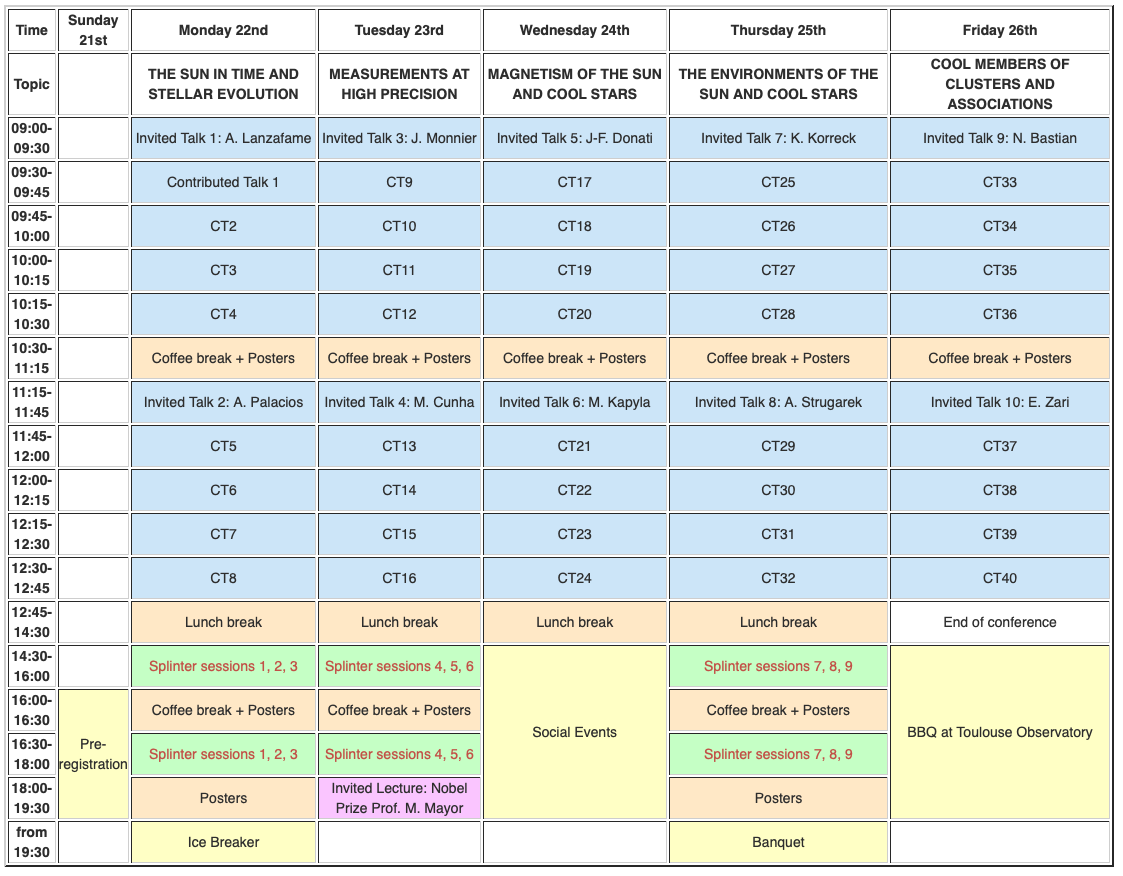
\includegraphics[width=1.10\textheight]{images/schedule.png}
\end{center}

\end{landscape}


\mainmatter


\chapter*{Talks}
\addcontentsline{toc}{chapter}{Talks}
  
    \section[Internal transport processes in stars and the Sun \newline(Ana Palacios)] { Internal transport processes in stars and the Sun }



%%% ========================
%%% Display authors and their affiliation(s)
%%% ========================
\begin{center}
{\large Ana Palacios}\\

%%% ===========================================
%%% Show schedule as a margin note for talks, or poster number for posters
%%% ===========================================


\marginnote{ Monday \\ 9:00 \\  (invited)  }[0cm]



\index{"Palacios" |textbf }
  
\vspace{2 mm}
\noindent Université de Montpellier / CNRS\\

\end{center}



%%% ===========
%%% Display abstract
%%% ===========
  
\vspace{2 mm}
  \noindent Internal transport processes are known to be at play in (cool) stars of all masses, and manifest through their impact on the surface chemical, rotational and magnetic evolution of stars, as well as through their shaping of the chemical and rotation gradients inside the stars as revealed by asteroseismology. In this talk I will give an updated overview of the recent progress made on the front of theory, modeling and observations concerning the  transport processes in stellar interiors.
    
%%% separation with a double line
\noindent\doubleline
   
    \section[A new generation of evolutionary and seismic solar models \newline(Gaël Buldgen)] { A new generation of evolutionary and seismic solar models }



%%% ========================
%%% Display authors and their affiliation(s)
%%% ========================
\begin{center}
{\large Gaël Buldgen (1)};{ \large  Patrick Eggenberger (2)}\\

%%% ===========================================
%%% Show schedule as a margin note for talks, or poster number for posters
%%% ===========================================


\marginnote{ Monday \\ 9:30 \\  }[0cm]



\index{"Buldgen" |textbf }\index{"Eggenberger" } 
  
\vspace{2 mm}
\noindent (1) Université de Genève; (2)  Université de Genève\\

\end{center}



%%% ===========
%%% Display abstract
%%% ===========
  
\vspace{2 mm}
  \noindent The Sun is the most observed star in the Universe. Thanks to this privileged status, it plays a key calibrator role for stellar physics, acting as a laboratory to test fundamental physical ingredients used in theoretical computations. Therefore, any refinement of the recipe of solar models will impact the ingredients for all models of solar-type stars. Following the revision of the solar abundances by Asplund and collaborators in 2005, confirmed in 2009, 2015 and 2021, the standard recipe of solar models has been put under question regarding both microscopic and macroscopic ingredients. In this talk, we will present results of new generations of both solar evolutionary and seismic models. We will show how evolutionary models taking into account the effects of rotation and magnetic fields can reproduce both the internal rotation, the lithium surface abundance and the helium abundance in the convective zone of the Sun. Furthermore, we will present a new approach to compute seismic solar models from iterative Ledoux discriminant inversions. We will show how such seismic models can be used to gain insights on the temperature gradient close to the base of the convective zone, where the robustness of opacity tables has been questioned. Combining both approaches will thus provide us key constraints on the required revision of physical ingredients to solve the long lasting solar modeling problem that followed the abundance revision in the early 2000s.
    
%%% separation with a double line
\noindent\doubleline
   
    \section[Solar neutrino fluxes show the signature of planet formation processes \newline(Masanobu Kunitomo)] { Solar neutrino fluxes show the signature of planet formation processes }



%%% ========================
%%% Display authors and their affiliation(s)
%%% ========================
\begin{center}
{\large Masanobu Kunitomo (1)};{ \large  Tristan Guillot (2)};{ \large  Gaël Buldgen (3)}\\

%%% ===========================================
%%% Show schedule as a margin note for talks, or poster number for posters
%%% ===========================================


\marginnote{ Monday \\ 9:45 \\  }[0cm]



\index{"Kunitomo" |textbf }\index{"Guillot" } \index{"Buldgen" } 
  
\vspace{2 mm}
\noindent (1) Kurume University; (2)  Observatoire de la Côte d'Azur; (3)  University of Geneva\\

\end{center}



%%% ===========
%%% Display abstract
%%% ===========
  
\vspace{2 mm}
  \noindent Solar evolutionary models are thus far unable to reproduce spectroscopic, helioseismic and neutrino constraints consistently, resulting in the so-called solar modeling problem. In parallel, planet formation models predict that the evolving composition of the protosolar disk, and thus, of the accreted gas by the proto-Sun must have been variable. In this talk, we show that solar evolutionary models including a realistic planet formation scenario lead to an increased core metallicity of up to 5\%, implying that accurate neutrino flux  measurements are sensitive to the initial stages of the formation of the Solar System. We demonstrate that in addition to macroscopic transport and increased opacities at the base of the convective envelope, the formation history of the Solar System constitutes a key element to resolve the current crisis of solar models.
    
%%% separation with a double line
\noindent\doubleline
   
    \section[Age or activity? Constraining evolutionary models with Li-depletion and rotation \newline(A. S. Binks)] { Age or activity? Constraining evolutionary models with Li-depletion and rotation }



%%% ========================
%%% Display authors and their affiliation(s)
%%% ========================
\begin{center}
{\large A. S. Binks (1)};{ \large  R. D. Jeffries (2)};{ \large  G. G. Sacco (3)};{ \large  R. J. Jackson (4)};{ \large  L. Cao (5)};{ \large  A. Bayo (6)};{ \large  M. Bergemann (7)};{ \large  R. Bonito (8)};{ \large  G. Gilmore (9)};{ \large  A. Gonneau (10)};{ \large  F. Jiminéz-Esteban (11)};{ \large  L. Morbidelli (12)};{ \large  S. Randich (13)};{ \large  V. Roccatagliata (14)};{ \large  R. Smiljanic (15)};{ \large  S. Zaggia (16)}\\

%%% ===========================================
%%% Show schedule as a margin note for talks, or poster number for posters
%%% ===========================================


\marginnote{ Monday \\ 10:00 \\  }[0cm]



\index{"Binks" |textbf }\index{"Jeffries" } \index{"Sacco" } \index{"Jackson" } \index{"Cao" } \index{"Bayo" } \index{"Bergemann" } \index{"Bonito" } \index{"Gilmore" } \index{"Gonneau" } \index{"Jiminéz-Esteban" } \index{"Morbidelli" } \index{"Randich" } \index{"Roccatagliata" } \index{"Smiljanic" } \index{"Zaggia" } 
  
\vspace{2 mm}
\noindent (1) MIT Kavli Institute for Astrophysics and Space Research, Massachusetts Institute of Technology \& Astrophysics Group, School of Chemical and Physical Sciences, Keele University; (2)  MIT Kavli Institute for Astrophysics and Space Research, Massachusetts Institute of Technology; (3)  INAF – Osservatorio Astrofisico di Arcetri; (4)  MIT Kavli Institute for Astrophysics and Space Research, Massachusetts Institute of Technology; (5)  4055 McPherson Laboratory, 140 West 18th Avenue, Columbus, Ohio 43210-1173, USA; (6)  Instituto de Física y Astronomía, Fac. de Ciencias, U de Valparaíso; (7)  Galaxies \& Cosmology Department, Max Planck Institute for Astronomy, Heidelberg \& Niels Bohr Institute, University of Copenhagen; (8)  INAF – Osservatorio Astronomico di Palermo; (9)  Institute of Astronomy, University of Cambridge; (10)  Institute of Astronomy, University of Cambridge; (11)  Nicolaus Copernicus Astronomical Center, Polish Academy of Sciences; (12)  INAF – Osservatorio Astrofisico di Arcetri; (13)  INAF – Osservatorio Astrofisico di Arcetri; (14)  Dipartimento di Fisica “Enrico Fermi”, Universitá di Pisa; (15)  Centro de Astrobiología (INTA-CSIC), Madrid; (16)  INAF – Osservatorio Astronomico di Padova\\

\end{center}



%%% ===========
%%% Display abstract
%%% ===========
  
\vspace{2 mm}
  \noindent Something's not right! Standard stellar models are clearly at odds with observations of colour-magnitude diagrams (CMDs) and Li-depletion patterns of pre main sequence (PMS) stars in clusters, and mounting evidence is suggesting inflation in low-mass stars - caused by strong dynamo-driven magnetic fields and/or cool starspots - leads to older inferred isochronal ages, in turn delaying the onset of Li-depletion, prompting a new generation of "magnetic models".

In this talk I'll pose a simple question: "Can any model provide good simultaneous fits of the CMD and Li-depletion patterns observed in clusters?"

By kinematically selecting high-probability members of 5 clusters from the Gaia-ESO Survey, with ages between  5-150 Myr we examine both standard and magnetic models by fitting isochrones and visually assessing the Li-pattern. We find: (1) standard models provide under-luminous fits at low-masses and can't capture the early stages of Li-depletion; (2) magnetic models are consistently 1.5-2 times older and better match Li-depletion; (3) strong degeneracy between magnetic activity and age.

Using TESS 30-min lightcurves we compiled rotation periods. Among the K-stars in the older clusters we find the brightest and least Li-depleted are the fastest rotators, demonstrating the classic “Li-rotation connection” for the first time at $\sim$35 Myr in NGC 2547, and find some evidence that it exists in the early M-stars of NGC 2264 at <10 Myr.
    
%%% separation with a double line
\noindent\doubleline
   
    \section[Exploring waves properties with multi-dimensional hydrodynamical simulations: from solar-type stars to intermediate-mass stars \newline(A. Le Saux)] { Exploring waves properties with multi-dimensional hydrodynamical simulations: from solar-type stars to intermediate-mass stars }



%%% ========================
%%% Display authors and their affiliation(s)
%%% ========================
\begin{center}
{\large A. Le Saux (1)};{ \large  T. Guillet (2)};{ \large  I. Baraffe (3)};{ \large  D. G. Vlaykov (4)};{ \large  T. Constantino (5)};{ \large  J. Pratt (6)};{ \large  T. Goffrey (7)};{ \large  M. Sylvain (8)};{ \large  V. Réville (9)};{ \large  A. S. Brun (10)}\\

%%% ===========================================
%%% Show schedule as a margin note for talks, or poster number for posters
%%% ===========================================


\marginnote{ Monday \\ 10:15 \\  }[0cm]



\index{"Saux" |textbf }\index{"Guillet" } \index{"Baraffe" } \index{"Vlaykov" } \index{"Constantino" } \index{"Pratt" } \index{"Goffrey" } \index{"Sylvain" } \index{"Réville" } \index{"Brun" } 
  
\vspace{2 mm}
\noindent (1) Physics and Astronomy, University of Exeter \& ENS-Lyon, CRAL, Université de Lyon; (2)  Physics and Astronomy, University of Exeter; (3)  Physics and Astronomy, University of Exeter \& ENS-Lyon, CRAL, Université de Lyon; (4)  Physics and Astronomy, University of Exeter; (5)  Physics and Astronomy, University of Exeter; (6)  Department of Physics and Astronomy, Georgia State University; (7)  Centre for Fusion, Space and Astrophysics, Department of Physics, University of Warwick; (8)  Physics and Astronomy, University of Exeter; (9)  Institut de Recherche en Astrophysique et Planétologie, CNRS, UPS, CNES; (10)  AIM, CEA, CNRS, Universités Paris et Paris-Saclay.\\

\end{center}



%%% ===========
%%% Display abstract
%%% ===========
  
\vspace{2 mm}
  \noindent The importance of waves propagating in the stars is twofold. First, they offer a great opportunity to unveil stellar internal structure and dynamics thanks to the observation of oscillations modes of stars, this is the field of asteroseismology. Secondly, they have an impact on the internal structure and evolution of stars as they can transport angular momentum, energy and chemical elements between different region of the star. In this presentation I would like to particularly focus on internal gravity waves (IGW). Observation of these waves remain challenging and their properties in stellar interiors remain poorly constrained. These properties of IGW are inherently 3D, non-linear and anisotropic. Consequently, multi-dimensional simulations are needed in order to test theoretical models and guide observations! This is essential for past, present and future missions such as Kepler, TESS or PLATO. 
In this talk, I will present a study of IGW in solar-like stars based on multi-dimensional stellar structure models preformed with a fully compressible hydrodynamics time implicit code, the MUSIC code. I will discuss how an artificial increase of the stellar luminosity and of the thermal diffusivity by several orders of magnitudes impact the waves properties. Our results suggest that this technique affect the excitation of IGW, because of an impact on convective motions and overshooting, but also their damping. This is of particular importance when studying mixing and stellar rotation. I will also present preliminary results for IGW propagating in the radiative envelope of intermediate mass stars with convective cores.
    
%%% separation with a double line
\noindent\doubleline
   
    \section[Magneto-rotational evolution of low-mass stars \newline(Alessandro C. Lanzafame)] { Magneto-rotational evolution of low-mass stars }



%%% ========================
%%% Display authors and their affiliation(s)
%%% ========================
\begin{center}
{\large Alessandro C. Lanzafame}\\

%%% ===========================================
%%% Show schedule as a margin note for talks, or poster number for posters
%%% ===========================================


\marginnote{ Monday \\ 11:15 \\  (invited)  }[0cm]



\index{"Lanzafame" |textbf }
  
\vspace{2 mm}
\noindent Dipartimento di Fisica e Astronomia, Università di Catania \& INAF - Osservatorio Astrofisico di Catania\\

\end{center}



%%% ===========
%%% Display abstract
%%% ===========
  
\vspace{2 mm}
  \noindent I will review some of the exciting developments that have occurred in the last few years regarding the evolution of rotation and magnetic field of low-mass stars, from pre-main sequence to late main sequence. I will focus on the evidence of distinct magneto-rotational regimes in the early phase of stellar evolution and of rapid transitions between them. Such evidence challenges a dependence on rotation only and suggests an important role of the rotational history in the early phase of the magneto-rotational evolution. The rotational evolution of one of these regimes, the slow-rotator one, can be described  to a satisfactory level of accuracy and I will outline the role of the core-envelope coupling in the first 1 Gyr. Many other issues remain unsolved and puzzling, like the conditions leading to the ultra-fast rotator regime, and the role of magnetic fields in the stellar radius inflation problem and on the lithium depletion pattern. Major contributions to these topics comes from space missions like Gaia, CoRot, Kepler, and TESS, combined with ground-based photometric and spectroscopic surveys and observations, as well as from Zeeman Doppler Imaging investigations. The most recent contributions come from Gaia DR3, which provides rotational periods for some 500 000 stars and chromospheric activity for some 2M stars.
    
%%% separation with a double line
\noindent\doubleline
   
    \section[New insights into late stages of the evolution of solar-mass stars thanks to intrinsic and extrinsic stars \newline(Sophie Van Eck)] { New insights into late stages of the evolution of solar-mass stars thanks to intrinsic and extrinsic stars }



%%% ========================
%%% Display authors and their affiliation(s)
%%% ========================
\begin{center}
{\large Sophie Van Eck (1)};{ \large  Shreeya Shetye (2)};{ \large  Drisya Karinkuzhi (3)};{ \large  Stephane Goriely (4)};{ \large  Lionel Siess (5)};{ \large  Alain Jorissen (6)}\\

%%% ===========================================
%%% Show schedule as a margin note for talks, or poster number for posters
%%% ===========================================


\marginnote{ Monday \\ 11:45 \\  }[0cm]



\index{"Eck" |textbf }\index{"Shetye" } \index{"Karinkuzhi" } \index{"Goriely" } \index{"Siess" } \index{"Jorissen" } 
  
\vspace{2 mm}
\noindent (1) IAA, Université Libre de Bruxelles; (2)  Laboratory of Astrophysics, Ecole Polytechnique Fédérale de Lausane; (3)  Indian Institute of Science, Bangalore; (4)  IAA, Université Libre de Bruxelles; (5)  IAA, Université Libre de Bruxelles; (6)  IAA, Université Libre de Bruxelles\\

\end{center}



%%% ===========
%%% Display abstract
%%% ===========
  
\vspace{2 mm}
  \noindent The foundations of stellar nucleosynthesis have been established more than 70 years ago and since then, many progresses have taken place, in particular concerning the heavy-element nucleosynthesis in late stages of the evolution of solar-mass stars. Targeting key-elements, including radio-isotopes, in both intrinsic and extrinsic stars, the latter constituting "cold cases" and useful probes of a past nucleosynthesis, allows to better understand chemical element production by stars with masses as low as 1 Msun during their evolved phases. Given their numerical importance, these stars are major contributors to the chemical evolution of the Galaxy.
    
%%% separation with a double line
\noindent\doubleline
   
    \section[The X-ray activity-rotation-age relation of M dwarfs and its mass dependence \newline(Enza Magaudda)] { The X-ray activity-rotation-age relation of M dwarfs and its mass dependence }



%%% ========================
%%% Display authors and their affiliation(s)
%%% ========================
\begin{center}
{\large Enza Magaudda (1)};{ \large  Beate Stelzer (2)};{ \large  Stefanie Raetz (3)};{ \large   Mara Salvato (4)};{ \large  Julien Wolf (5)}\\

%%% ===========================================
%%% Show schedule as a margin note for talks, or poster number for posters
%%% ===========================================


\marginnote{ Monday \\ 12:00 \\  }[0cm]



\index{"Magaudda" |textbf }\index{"Stelzer" } \index{"Raetz" } \index{"Salvato" } \index{"Wolf" } 
  
\vspace{2 mm}
\noindent (1) Institut für Astronomie und Astrophysik, Eberhard-Karls Universitat Tübingen; (2)  Institut für Astronomie und Astrophysik, Eberhard-Karls Universitat Tübingen and INAF- Osservatorio Astronomico di Palermo; (3)  Institut für Astronomie und Astrophysik, Eberhard-Karls Universitat Tübingen; (4) 
Max-Planck-Institut für extraterrestrische Physik and Exzellenzcluster ORIGINS, Garching; (5)  Max-Planck-Institut für extraterrestrische Physik and Exzellenzcluster ORIGINS, Garching\\

\end{center}



%%% ===========
%%% Display abstract
%%% ===========
  
\vspace{2 mm}
  \noindent The activity of the Sun and solar-like stars is driven by an $\alpha\Omega-$dynamo, according to which the combination of differential rotation and convective motions of the outer atmospheric envelope continuously regenerates the magnetic field that manifests itself in the form of powerful optical, UV, and X-ray radiation.
The study of the X-ray activity-rotation-age relation therefore probes both the stellar dynamo and spin evolution. Moreover, how the X-ray emission varies with stellar age is of great importance for planetary atmospheres and yields information about how stellar X-rays affect their evolution. M dwarfs are also known to be magnetically active, but the physical mechanism is poorly understood. In this talk, I present the largest uniform sample of M dwarfs (302 stars) consisting of observations taken with XMM-Newton, Chandra, and K2 combined with X-ray and rotation data from the literature. With the use of spin models we compared the evolution of the predicted rotation periods ($P_{\rm rot}$) with our results on the empirical $L_{\rm x} - P_{\rm rot}$ relation to provide an estimate for the age decay of X-ray luminosity and we compare it to the few stars with known age and X-ray emission.  
Later, new X-ray data from eROSITA and rotation periods extracted from TESS light curves doubled our sample of M dwarfs, allowing us to put a quantitative constraint on the mass dependence of the X-ray emission, and to determine the drop in activity level with respect to pre-main sequence stars.  Finally, we quantified the X-ray variability of this large sample by comparing the $L_{\rm x}$ from eROSITA and ROSAT measurements and we examined the sensitivity improvements with eROSITA. In particular, eROSITA is able to detect faint M dwarfs that are visible by ROSAT only during flaring emission and it is also sensitive for slower rotating M dwarfs in the unsaturated regime of the $L{\rm x}-P_{\rm rot}$ relation ($P_{\rm rot}\geq10$ d) that is inaccessible to TESS.
    
%%% separation with a double line
\noindent\doubleline
   
    \section[Young stars and their disc - A short but complex story \newline(Louis Amard)] { Young stars and their disc - A short but complex story }



%%% ========================
%%% Display authors and their affiliation(s)
%%% ========================
\begin{center}
{\large Louis Amard (1)};{ \large  Sean P. Matt (2)}\\

%%% ===========================================
%%% Show schedule as a margin note for talks, or poster number for posters
%%% ===========================================


\marginnote{ Monday \\ 12:15 \\  }[0cm]



\index{"Amard" |textbf }\index{"Matt" } 
  
\vspace{2 mm}
\noindent (1) Université Paris-Saclay, Université de Paris, CEA, CNRS, Astrophysique, Instrumentation et Modélisation Paris-Saclay, F-91191, Gif-sur-Yvette; (2) 
University of Exeter, Physics and Astrophysics dept, Exeter, EX44QL, UK\\

\end{center}



%%% ===========
%%% Display abstract
%%% ===========
  
\vspace{2 mm}
  \noindent During their formation, most young stars are surrounded by a protoplanetary disc. The angular momentum evolution of these systems is quite complex but still poorly understood despite a lot of effort and some recent breakthrough. 
For instance, observations indicate that stars with a disc tend to rotate more slowly even though they accrete angular momentum, and during the first 10 Myr, young low-mass stars do not seem to spin-up while they are expected to contract.
To tackle this long-standing problem, I will present state-of-the-art stellar evolution models with accretion which include a self-consistent treatment of angular momentum evolution thanks to the results of dynamical multi-D MHD simulations. 
We explore the observed range of several parameter, such as the accretion rate history, the composition and the thermodynamics of the accreted material, as well as the large scale magnetic field strength of the star. 
I will show that the observed spin rate, the long-standing disc-locking problem, as well as other observed properties of very young stars can be explained by the complex interplay of the different processes.
    
%%% separation with a double line
\noindent\doubleline
   
    \section[Pre Main Sequence stellar and accretion properties in the era of ULLYSES and PENELLOPE \newline(Carlo F. Manara)] { Pre Main Sequence stellar and accretion properties in the era of ULLYSES and PENELLOPE }



%%% ========================
%%% Display authors and their affiliation(s)
%%% ========================
\begin{center}
{\large Carlo F. Manara}\\

%%% ===========================================
%%% Show schedule as a margin note for talks, or poster number for posters
%%% ===========================================


\marginnote{ Monday \\ 12:30 \\  }[0cm]



\index{"Manara" |textbf }
  
\vspace{2 mm}
\noindent ESO\\

\end{center}



%%% ===========
%%% Display abstract
%%% ===========
  
\vspace{2 mm}
  \noindent Determining the stellar and accretion properties of young low-mass Pre-Main-Sequence stars is vital to better understand stellar evolution, and the general evolution of protoplanetary disks and planet formation. The last years are seeing a flourishing of possibilities to properly determine these stellar and accretion properties, combining spectroscopic observations from ground-based telescopes (e.g., the large programme with the Very Large Telescope, PENELLOPE) with space-based (HST) spectra, mainly from the ULLYSES public survey, targeting 82 low-mass ($M_\star \lesssim 2 M_\odot$) young (age$<$10 Myr) stars at UV wavelengths. 
I will present the main results obtained from these programs, and how these are leading to a better understanding of how we can determine stellar and accretion properties of young stars, to better decipher how stars and planets form.
    
%%% separation with a double line
\noindent\doubleline
   
    \section[The legacy of space-based asteroseismolgy \newline(Margarida Cunha)] { The legacy of space-based asteroseismolgy }



%%% ========================
%%% Display authors and their affiliation(s)
%%% ========================
\begin{center}
{\large Margarida Cunha}\\

%%% ===========================================
%%% Show schedule as a margin note for talks, or poster number for posters
%%% ===========================================


\marginnote{ Tuesday \\ 9:00 \\  (invited)  }[0cm]



\index{"Cunha" |textbf }
  
\vspace{2 mm}
\noindent Instituto de Astrofísica e Ciências do Espaço, Universidade do Porto, Portugal\\

\end{center}



%%% ===========
%%% Display abstract
%%% ===========
  
\vspace{2 mm}
  \noindent The detection of solar-like oscillations in thousands of cool stars enabled by the ultra-precise photometry of space missions such as CoRoT, Kepler, and TESS, has empowered research in stellar physics and stellar internal dynamics, moving forward our understanding of stellar evolution. This dramatic change has also a direct impact on research fields that depend on the accurate characterisation of stellar properties, such as exoplanet 
research and Galactic archaeology.

In this talk I will review some of the key advances brought by space-based asteroseismic data to our understanding of cool stars, discuss key issues that are still under debate and briefly look into the future. 

    
%%% separation with a double line
\noindent\doubleline
   
    \section[Cool stars and their planets with the PLATO mission \newline(S. Aigrain)] { Cool stars and their planets with the PLATO mission }



%%% ========================
%%% Display authors and their affiliation(s)
%%% ========================
\begin{center}
{\large S. Aigrain (1)}\\

%%% ===========================================
%%% Show schedule as a margin note for talks, or poster number for posters
%%% ===========================================


\marginnote{ Tuesday \\ 9:30 \\  }[0cm]



\index{"Aigrain" |textbf }
  
\vspace{2 mm}
\noindent (1) University of Oxford\\

\end{center}



%%% ===========
%%% Display abstract
%%% ===========
  
\vspace{2 mm}
  \noindent PLATO (PLAnetary Transits and Oscillations of stars) is ESA's M3 mission, scheduled for launch in late 2026. Using 26 cameras with 12 cm aperture and partially overlapping fields of view, it will spend at least 4 years performing high-precision, high-cadence, long-baseline photometry of bright stars, simultaneously searching for planetary transits and stellar oscillations. PLATO will provide the first large sample of well-characterised small planets up to intermediate orbital periods, including terrestrial planets in the habitable zone of solar-like stars. Thanks to its integrated approach (transit detection, asteroseismology and ground-based follow-up are all part of the baseline mission), it will determine the masses, radii and ages of both the host stars and their planets to high accuracy. This will enable detailed tests of theoretical models of the formation and evolution of planets and planetary systems. Many of the planets that PLATO will discover will also be well-suited for atmospheric characterisation from the ground and/or space. 
In this talk I will give a brief overview of the payload, the mission and its expected scientific yield and impact. One of the key challenges for PLATO will be to disentangle the planetary signals of interest from low-level stellar variability and residual instrumental effects. I will discuss how we can exploit PLATO's unique multi-camera strategy to build data-driven models that can help overcome this challenge.
    
%%% separation with a double line
\noindent\doubleline
   
    \section[Butterfly diagrams in sun-like stars using asteroseismology \newline(M. Bazot)] { Butterfly diagrams in sun-like stars using asteroseismology }



%%% ========================
%%% Display authors and their affiliation(s)
%%% ========================
\begin{center}
{\large M. Bazot  (1)};{ \large  M. B. Nielsen  (2)};{ \large  D. Mary  (3)};{ \large  J. Christensen-Dalsgaard  (4)};{ \large  O. Benomar  (5)};{ \large  P. Petit  (6)};{ \large  L. Gizon  (7)};{ \large  K. R. Sreenivasan  (8)};{ \large  T. R. White  (9)}\\

%%% ===========================================
%%% Show schedule as a margin note for talks, or poster number for posters
%%% ===========================================


\marginnote{ Tuesday \\ 9:45 \\  }[0cm]



\index{"Bazot" |textbf }\index{"Nielsen" } \index{"Mary" } \index{"Christensen-Dalsgaard" } \index{"Benomar" } \index{"Petit" } \index{"Gizon" } \index{"Sreenivasan" } \index{"White" } 
  
\vspace{2 mm}
\noindent (1) Heidelberg Institute for Theoretical Studies (HITS gGmbH); (2)  University of Birmingham; (3)  Laboratoire Lagrange, Université Côte d'Azur, Observatoire de la Côte d'Azur, CNRS; (4)  Stellar Astrophysics Centre, Department of Physics and Astronomy, Aarhus University; (5)  The University of Tokyo and NAOJ, Tokyo; (6)  IRAP/Université de Toulouse, CNRS; (7)  Max-Planck-Institut/Institut für Astrophysik/New York University Abu Dhabi; (8)  New York University; (9)  University of Sydney\\

\end{center}



%%% ===========
%%% Display abstract
%%% ===========
  
\vspace{2 mm}
  \noindent Stellar activity is a long-standing problem in stellar physics, pertaining to the solar dynamo model, that is the mechanism that generates the stellar magnetic field. In the Sun, the variations of the latitudinal coordinates of the surface active regions with time, the so-called butterfly diagram, are a key observational constraint. They are an important test for benchmarking solar dynamo models. In other stars, although direct imaging does not allow to resolve their surfaces, it is sometimes possible to reconstruct activity maps for certain classes of stars. As a general rule, this is particularly difficult for Sun-like stars, which are slowly rotating and do not often exhibit a strong magnetic field. In this presentation, I explain how to perform such a reconstruction for a Sun-like star using Kepler time series and asteroseismic analysis. This has been done for the first time for HD 173701 (KIC 8006161). The method rests upon combining classical period estimation using the low-frequency signal in the data and asteroseismic measurements of latitudinal differential rotation using asteroseismology. This was accomplished using an array of methods from computational Statistics. They allowed us to invert for a butterfly diagram over the four years of the Kepler mission, with statistically significant variations observed in the latitude of the active regions of this star. I discuss the limitations of the method as well as the important perspective it opens for the characterization of stellar activity. I replace the significance of this finding in the context of the upcoming PLATO mission.
    
%%% separation with a double line
\noindent\doubleline
   
    \section[Rotational Characterization of TESS Stars with Deep Learning \newline(Zachary R. Claytor)] { Rotational Characterization of TESS Stars with Deep Learning }



%%% ========================
%%% Display authors and their affiliation(s)
%%% ========================
\begin{center}
{\large Zachary R. Claytor};{ \large  Jennifer L. van Saders}\\

%%% ===========================================
%%% Show schedule as a margin note for talks, or poster number for posters
%%% ===========================================


\marginnote{ Tuesday \\ 10:00 \\  }[0cm]



\index{"Claytor" |textbf }\index{"Saders" } 
  
\vspace{2 mm}
\noindent University of Hawaii\\

\end{center}



%%% ===========
%%% Display abstract
%%% ===========
  
\vspace{2 mm}
  \noindent The TESS mission has the potential to probe stellar rotation in millions of stars across the entire sky, but mission systematics—instrumental noise, observing gaps, and changes in detector sensitivity—have prevented recovery of rotation periods longer than 13.7 days. We used deep learning to see through TESS systematics and recover periods from year-long light curves. Our approach uses a training set of synthesized light curves from realistic star spot evolution simulations, with real light curve systematics from quiet TESS stars. Evaluating the network on real TESS data, we recovered periods for 20,000 cool dwarfs. The period distribution resembles the Kepler and K2 distributions, including periods up to 90 days. Using gyrochronology, we estimated masses, ages, and other fundamental stellar parameters for 5,000 TESS stars with APOGEE spectroscopy. We combine this with a similar sample from Kepler and show that we can use rotation-based ages to recover Galactic chemical evolution trends previously seen only in stars more massive or more evolved than the Sun. With rotation periods across the entire sky, we can characterize stars along many more lines of sight than before, enabling detailed study of the Galaxy’s stellar populations.
    
%%% separation with a double line
\noindent\doubleline
   
    \section[A four-year follow-up campaign of TRAPPIST-1 from the ground \newline(Elsa Ducrot)] { A four-year follow-up campaign of TRAPPIST-1 from the ground }



%%% ========================
%%% Display authors and their affiliation(s)
%%% ========================
\begin{center}
{\large Elsa Ducrot (1)};{ \large  Michaël Gillon (2)};{ \large  Eric Agol (3)};{ \large  the SPECULOOS team (4)}\\

%%% ===========================================
%%% Show schedule as a margin note for talks, or poster number for posters
%%% ===========================================


\marginnote{ Tuesday \\ 10:15 \\  }[0cm]



\index{"Ducrot" |textbf }\index{"Gillon" } \index{"Agol" } \index{"team" } 
  
\vspace{2 mm}
\noindent (1) CEA Saclay; (2)  University of Liège; (3)  University of Washington; (4)  University of Liège\\

\end{center}



%%% ===========
%%% Display abstract
%%% ===========
  
\vspace{2 mm}
  \noindent In this talk, we present the results from an extensive four-year long follow-up campaign of the TRAPPIST-1 system led from the ground with the SPECULOOS and Liverpool Telescopes. This represents 285 nights of observations, 228 new transits of the seven planets, and includes 3 months of daily monitoring of the star to study its photometric variability. 
First of all, to try to understand the origin of the existing inconsistency between K2 and Spitzer photometric variability, we derive the rotation period of the host star in the I+z band and use it to propose a spot variability model that would agree with the observations in each band and at the same time provide insights on the nature (proportion and temperature) of the photospheric heterogeneities on the surface of TRAPPIST-1, in a similar way as in Morris et al. (2018). From those outcomes we discuss the expected impact of stellar contamination on the planetary spectra via the transit light source effect. In parallel, we present our statistics of spot-like and faculae-like crossing events on all observed transits and relate them to the photometric modulations.
In addition, we analyze 269 new transits in order to (1) refine the planets' parameters using individual and global analyses and (2) derive precise transit timing variations for the seven planets. We show that recent timings (most recent ones from Nov 2021) of planet h seem to slightly deviate from the predictions by Agol et al. (2021), implying either that planet h's timings have an excess of outliers or that a 7-planet model is no longer a good fit, which could suggest the existence of a putative eighth planet. To figure this out, we show the results of new optimization runs with 7-planet and 8-planet models and including periodic orbit (P-O) - families of solutions to the N-body problem - constraints. Indeed, near-resonant planetary system such as TRAPPIST-1 are expected to reside in the dynamical neighborhood of stable P-Os (Antoniadou et al. (2020)) and such a configuration can be used to yield better constraints on the orbital elements.
Finally, we look at TRAPPIST-1's flaring activity. On one hand, we compute flare occurrence rates and energies to compute flare frequency distribution and complement the work initiated by Ducrot et al. (2020) on placing the TRAPPIST-1 planets relative to the abiogenesis zone introduced by Rimer et al. (2018). On the other hand, we seek correlations between flaring events and periodic photometric variability to state whether the observation of Morris et al (2018) claiming that visible flares seem to occur preferentially when the star is bright, and when the brightness is increasing most rapidly, is confirmed or not.
    
%%% separation with a double line
\noindent\doubleline
   
    \section[Revealing the Surfaces of Stars with Interferometric Imaging \newline(Rachael Roettenbacher)] { Revealing the Surfaces of Stars with Interferometric Imaging }



%%% ========================
%%% Display authors and their affiliation(s)
%%% ========================
\begin{center}
{\large Rachael Roettenbacher}\\

%%% ===========================================
%%% Show schedule as a margin note for talks, or poster number for posters
%%% ===========================================


\marginnote{ Tuesday \\ 11:15 \\  (invited)  }[0cm]



\index{"Roettenbacher" |textbf }
  
\vspace{2 mm}
\noindent Yale University\\

\end{center}



%%% ===========
%%% Display abstract
%%% ===========
  
\vspace{2 mm}
  \noindent Since the first stellar diameters were resolved with interferometry in the early twentieth century, the technique has revealed the angular extent of hundreds of stars.  Knowing the size of a star on the sky and its distance from Earth has allowed for straight-forward measurements of fundamental stellar parameters.  Measuring a stellar diameter can be achieved with just two telescopes which make a single baseline, but today's interferometric arrays allow for multiple baselines to be observed at once.  Combining the light from three telescopes at once allows for the observations of closure phases, which highlight asymmetries of the target.  By increasing the number of telescopes and observations and the size of baselines, sufficient data can be obtained to not just resolve the size of stars, but image details on their surfaces.  In recent years, a number of studies have shown that interferometric imaging is capable of capturing the surface details of a wide variety of stars as they appear on the sky.  I will present a review of the images obtained to date, particularly noting those of cool stars, like asymptotic giant, supergiant, and magnetically active stars.  I will also detail the advantages of the method compared to other imaging techniques and of utilizing stellar surface images.
    
%%% separation with a double line
\noindent\doubleline
   
    \section[Sub-AU study of CI Tau with VLTI/GRAVITY:
The key to link stellar activities, disks and planets.
 \newline(A. Soulain)] { Sub-AU study of CI Tau with VLTI/GRAVITY:
The key to link stellar activities, disks and planets.
 }



%%% ========================
%%% Display authors and their affiliation(s)
%%% ========================
\begin{center}
{\large A. Soulain};{ \large  J. Bouvier};{ \large  K. Perraut}\\

%%% ===========================================
%%% Show schedule as a margin note for talks, or poster number for posters
%%% ===========================================


\marginnote{ Tuesday \\ 11:45 \\  }[0cm]



\index{"Soulain" |textbf }\index{"Bouvier" } \index{"Perraut" } 
  
\vspace{2 mm}
\noindent Univ. Grenoble Alpes, CNRS, IPAG, 38000 Grenoble, France\\

\end{center}



%%% ===========
%%% Display abstract
%%% ===========
  
\vspace{2 mm}
  \noindent For a few million years after the gravitational collapse that led to their formation; young stellar systems remain surrounded by a circumstellar disk from which planets form. ALMA and VLT/SPHERE have provided spectacular images of the planet-forming disks on a scale of a few 10 au (Garufi et al. 2017) and; even more recently; led to the direct detection of forming planets within the disk (Benisty et al. 2021). In contrast; the exploration of the innermost disk regions ($\lesssim$ 1 au) has remained quite challenging so far. Moreover; the Kepler satellite has revealed that the most ubiquitous planetary systems consist of compact strings of super-Earth and mini-Neptunes orbiting close to their host star (Porb $\lesssim$ 100 days; e.g.; Otegi et al. 2022;). It is; therefore; crucial to investigate the physics of the star-planet-inner disk interaction in young stars; not only for the role it plays in the early evolution of solar-type stars (e.g.; accretion/ejection; angular momentum; etc.) but also to determine the environmental conditions that prevail at the time of planetary formation. This is a necessary step towards understanding the formation of the plethora of compact inner low-mass planetary systems observed across the Galaxy. CI Tau is so far the only pre-main sequence star still accreting from its surrounding disk (classical T-Tauri star) claimed to host a hot Jupiter planet. However; the periodic radial velocity variation could result from magnetospheric accretion onto the star rather than from an orbiting body (Donati et al. 2020). The most interesting aspect of CI Tau regards its extreme magnetic field (3.7 kG) that disrupts the inner gaseous disk and generates accretion funnel flows down to the stellar surface. We propose to present our investigation about the inner region of CI Tau; aiming at reconnecting the different spatial scales of the system down to a few stellar radii ($\lesssim$ 0.1 AU).

Method: We investigated this puzzling question using the long-baseline interferometry technique; the only way to probe the inner region of the system at sub-AU precision. Thanks to the high spectral resolution of VLTI/GRAVITY (R=4000); we are both sensitive to the emitting dusty part of the inner rim (K-band continuum); and the magnetosphere itself traced by the Br$\gamma$ emission line.
    
Results: In the continuum; we characterise the disk's inner rim; which appeared to be disconnected from the outer disk with a large misalignment both in inclination and position angle. We report an internal rim position at 0.17 $\pm$ 0.02 AU; remarkably more significant than the theoretical sublimation radius of 0.03-0.06 AU. Such difference could infer the presence of a planet carving the inner part of the disk; as recently supported by hydrodynamical simulation (Muley et al. 2021). The non-zero closure phases measured by GRAVITY suggest an important asymmetry in the disk: the southwest side appears brighter than the northeast. Such difference argues in favour of an inclined disk where the brilliant (and farthest) part is seen from the bottom (distant observer point of view). We confirmed such behaviours using radiative transfer modelling with RADMC3d. In the Br$\gamma$ line (2.1661 $\mu$m), our model suggests a bright but smaller emitting region than the thermal emission with a radius of 0.04 $\pm$ 0.01 AU (4 times smaller than the inner rim). Such characteristic is strongly supported by the magnetosphere accreting models developed in our team and will be presented for comparison. 
    
Conclusion: With GRAVITY; we characterise the inner disk of CI Tau with a sub-AU precision; allowing a direct comparison with the standard YSO's characteristic sizes such as sublimation; co-rotation or magnetic truncation radii. The existence of a larger than expected central cavity could be an observational signature of the well known 11.6 Mj planet (CI Tau b). The substantially detected misalignment between inner and outer disks constitutes a challenge for the modelling efforts and should be carefully investigated in the future.
    
%%% separation with a double line
\noindent\doubleline
   
    \section[Pre-main sequence stars in the time domain: insights from high-precision, space-borne photometry \newline(Laura Venuti)] { Pre-main sequence stars in the time domain: insights from high-precision, space-borne photometry }



%%% ========================
%%% Display authors and their affiliation(s)
%%% ========================
\begin{center}
{\large Laura Venuti};{ \large  Ann Marie Cody};{ \large  K2 team}\\

%%% ===========================================
%%% Show schedule as a margin note for talks, or poster number for posters
%%% ===========================================


\marginnote{ Tuesday \\ 12:00 \\  }[0cm]



\index{"Venuti" |textbf }\index{"Cody" } \index{"team" } 
  
\vspace{2 mm}
\noindent SETI Institute\\

\end{center}



%%% ===========
%%% Display abstract
%%% ===========
  
\vspace{2 mm}
  \noindent High-precision time series photometry provides a unique window into the dynamics of the inner disk regions (< 1 AU) around young stars (< 5-10 Myr). Exquisite surveys carried out with CoRoT, Kepler, and TESS have revealed a huge variety of photometric behaviors for young stellar objects, driven by variable mass accretion, stellar magnetic activity, or rapidly evolving circumstellar dust structures. This variety of behaviors, observed in each young cluster and star-forming region investigated from space, points to a coexistence of distinct paradigms of star-disk interaction that may govern different stages of pre-main sequence evolution. Thanks to the K2 mission, accurate time domain data for hundreds of young stars are now available for virtually every stage of protoplanetary disk lifetimes, across different stellar mass regimes from cool stars and beyond: surveyed regions range from rho Ophiuchi and the Lagoon Nebula ( 2 Myr), to NGC 2264 (3-5 Myr, monitored earlier with CoRoT), to Upper Scorpius (5-10 Myr). In this contribution, we discuss the insights provided by those campaigns into the time evolution of inner disks around young stars, and what these observations teach us regarding the stellar and circumstellar dynamics as a function of stellar mass and environmental conditions.
    
%%% separation with a double line
\noindent\doubleline
   
    \section[A Demographic TESS View of M-dwarf Activity: Flares, Rotation, and Ages \newline(Maximilian N. Günther)] { A Demographic TESS View of M-dwarf Activity: Flares, Rotation, and Ages }



%%% ========================
%%% Display authors and their affiliation(s)
%%% ========================
\begin{center}
{\large Maximilian N. Günther (1)};{ \large  TESS Science Team (2)}\\

%%% ===========================================
%%% Show schedule as a margin note for talks, or poster number for posters
%%% ===========================================


\marginnote{ Tuesday \\ 12:15 \\  }[0cm]



\index{"Günther" |textbf }\index{"Team" } 
  
\vspace{2 mm}
\noindent (1) European Space Agency (ESA); (2)  others\\

\end{center}



%%% ===========
%%% Display abstract
%%% ===========
  
\vspace{2 mm}
  \noindent While TESS searches for temperate cool star worlds, it also provides an unprecedented survey of their host's stellar activity. Especially stellar flares and coronal mass ejections (CMEs) can be a double-edged sword for M-dwarf exoplanets. On the one hand, these energetic outbursts are capable of shaping or stripping off planetary atmospheres; on the other hand, they might deliver the necessary trigger energy for origin-of-life chemistry. Here, I will highlight our study of all stellar flares from the TESS primary mission's 2 min cadence data of 230,000 stars, driven by a convolutional neural network. I will discuss our new demographic insights on M-dwarf flaring as a function of stellar type, age, rotation, spot coverage, and other factors. With an eye on exoplanets, I will link our findings to ozone sterilisation and prebiotic chemistry, identifying which worlds might lie in the "flaring sweet spot" for life. With future extended missions and 20 s cadence, M-dwarf activity studies can guide us further in understanding cool star vs. planet interactions.
    
%%% separation with a double line
\noindent\doubleline
   
    \section[Atmospheric retrievals of T dwarfs: clouds, composition, and clues to formation  \newline(Josefine Gaarn)] { Atmospheric retrievals of T dwarfs: clouds, composition, and clues to formation  }



%%% ========================
%%% Display authors and their affiliation(s)
%%% ========================
\begin{center}
{\large Josefine Gaarn (1)};{ \large  Ben Burningham (2)};{ \large  Jacqueline Faherty (3)};{ \large  Channon Visscher (4)};{ \large  Mark Marley (5)};{ \large  Eileen Gonzales (6)};{ \large  Emily Calamari (7)};{ \large  Daniella Bardalez Gagliuffi  (8)}\\

%%% ===========================================
%%% Show schedule as a margin note for talks, or poster number for posters
%%% ===========================================


\marginnote{ Tuesday \\ 12:30 \\  }[0cm]



\index{"Gaarn" |textbf }\index{"Burningham" } \index{"Faherty" } \index{"Visscher" } \index{"Marley" } \index{"Gonzales" } \index{"Calamari" } \index{"Gagliuffi" } 
  
\vspace{2 mm}
\noindent (1) University of Hertfordshire; (2)  University of Hertfordshire; (3)  American Museum of Natural History; (4)  Dordt University \& Space Science Institute; (5)  University of Arizona; (6)  Cornell University \& American Museum of Natural History; (7)  Graduate Center CUNY \& American Museum of Natural History; (8)  American Museum of Natural History \\

\end{center}



%%% ===========
%%% Display abstract
%%% ===========
  
\vspace{2 mm}
  \noindent Atmospheric retrievals of T dwarfs: clouds, composition, and clues to formation 
Brown dwarfs are often described as the low mass extension of the star formation process. In this scenario, we would expect the compositions of brown dwarfs to follow those of the wider stellar population. At the lowest masses, however, it is reasonable to ask whether some fraction of the brown dwarf population arises from similar processes to those that make planets. We will summarise progress and early results of a large retrieval study of T dwarfs comparing isolated objects and companions to stars, measuring atmospheric abundances with a view to constraining their compositions. We also report the frequency of cloudy atmospheres across a broad range of spectral types, with clouds getting more common towards later types. Finally, we will highlight the case of Ross-458c, potentially planetary mass T8 dwarf in orbit around a M0.5+M7 pair. In agreement with previous studies, we find the atmosphere of Ross-458c to best be described by a cloudy model. We find a very high CH4/H2O ratio of 1.97 $M_\pm$ 0.13, which is challenging to understand in terms of equilibrium chemistry and plausible C/O ratios. This value may be consistent with a C/O ratio  1.4 if the ${\rm CH_4}$ and ${\rm H_{2}O}$ abundances are quenched at the T=2000 K level, which would itself require vigorous vertical mixing. We explore the implications of these results for the origin of Ross-458c.
    
%%% separation with a double line
\noindent\doubleline
   
    \section[Doppler cross-correlation spectroscopy as a path to the detection of Earth-like planets - From CORAVEL to ESPRESSO via ELODIE  -  \newline(Michel Mayor)] { Doppler cross-correlation spectroscopy as a path to the detection of Earth-like planets - From CORAVEL to ESPRESSO via ELODIE  -  }



%%% ========================
%%% Display authors and their affiliation(s)
%%% ========================
\begin{center}
{\large Michel Mayor}\\

%%% ===========================================
%%% Show schedule as a margin note for talks, or poster number for posters
%%% ===========================================


\marginnote{ Tuesday \\ 18:15 \\  (invited)  }[0cm]



\index{"Mayor" |textbf }
  
\vspace{2 mm}
\noindent Geneva Observatory\\

\end{center}



%%% ===========
%%% Display abstract
%%% ===========
  
\vspace{2 mm}
  \noindent 
    
%%% separation with a double line
\noindent\doubleline
   
    \section[Exoplanets and life in the Universe \newline(Didier Queloz)] { Exoplanets and life in the Universe }



%%% ========================
%%% Display authors and their affiliation(s)
%%% ========================
\begin{center}
{\large Didier Queloz}\\

%%% ===========================================
%%% Show schedule as a margin note for talks, or poster number for posters
%%% ===========================================


\marginnote{ Tuesday \\ 19:00 \\  (invited)  }[0cm]



\index{"Queloz" |textbf }
  
\vspace{2 mm}
\noindent University of Cambridge and ETH Zürich \\

\end{center}



%%% ===========
%%% Display abstract
%%% ===========
  
\vspace{2 mm}
  \noindent The richness and diversity of planetary systems that have now been detected have modified our perspective on planet formation and our place in the Universe. They also represent an historical opportunity of perspectives and a compelling call to look for signs of life on these new worlds and to reflect on the origin of life in the Solar System. I will introduce the audience to the challenges and recent advances in this field, in the context of the new research centres set up at Cambridge and ETH-Z and how they address the origins of life on Earth and its prevalence in the Universe. 
    
%%% separation with a double line
\noindent\doubleline
   
    \section[Magnetic fields of late-type stars - an observational overview  \newline(Jean-Francois Donati)] { Magnetic fields of late-type stars - an observational overview  }



%%% ========================
%%% Display authors and their affiliation(s)
%%% ========================
\begin{center}
{\large Jean-Francois Donati}\\

%%% ===========================================
%%% Show schedule as a margin note for talks, or poster number for posters
%%% ===========================================


\marginnote{ Wednesday \\ 9:00 \\  (invited)  }[0cm]



\index{"Donati" |textbf }
  
\vspace{2 mm}
\noindent CNRS / Université de Toulouse\\

\end{center}



%%% ===========
%%% Display abstract
%%% ===========
  
\vspace{2 mm}
  \noindent My talk will outline the latest observational advances in detecting and characterizing magnetic fields of late-type stars, from young pre-main-sequence (PMS) to mature and evolved objects.  I will focus in particular on the latest magnetic measurements, for instance those of weakly-active M dwarfs and PMS stars collected over the last few years with the infrared spectropolarimeter SPIRou at the Canada-France-Hawaii Telescope, in the framework of the SPIRou Legacy Survey.  
    
%%% separation with a double line
\noindent\doubleline
   
    \section[What makes a stellar surface preferentially facular or spot dominated? \newline(Eliana M. Amazo-Gomez)] { What makes a stellar surface preferentially facular or spot dominated? }



%%% ========================
%%% Display authors and their affiliation(s)
%%% ========================
\begin{center}
{\large Eliana M. Amazo-Gomez};{ \large  Katja Poppenhaeger}\\

%%% ===========================================
%%% Show schedule as a margin note for talks, or poster number for posters
%%% ===========================================


\marginnote{ Wednesday \\ 9:30 \\  }[0cm]



\index{"Amazo-Gomez" |textbf }\index{"Poppenhaeger" } 
  
\vspace{2 mm}
\noindent Leibniz Institute for Astrophysics Potsdam AIP\\

\end{center}



%%% ===========
%%% Display abstract
%%% ===========
  
\vspace{2 mm}
  \noindent The photosphere of Sun-like stars have been found to display a smooth transition between being dominated by spots or by facular features. Our analysis indicates that the Sun lies in the transition between the spot and faculae domination regime. Some hypotheses have been explored suggesting that such surface manifestations may correlate with different magnetic dynamo modes. By using a recently developed method based on the Gradient of the Power Spectra (GPS), we quantified the ratio between faculae to spots signature based on solar and stellar light curves. We characterized a sample of 30 Sun-like stars which we have identified to have different levels of spot- or faculae-dominance on their surface. We analyzed the longitudinal magnetic field, additional activity indicators such as the S-Index from the calcium H\&K core line, H-alpha, and the Ca triplet in the near-infrared. We interpret the differences between having spot versus faculae dominated stellar surfaces.
    
%%% separation with a double line
\noindent\doubleline
   
    \section[Influence of Magnetic Cycles on Stellar Prominences and their Mass Loss Rates \newline(Sarah J. Faller)] { Influence of Magnetic Cycles on Stellar Prominences and their Mass Loss Rates }



%%% ========================
%%% Display authors and their affiliation(s)
%%% ========================
\begin{center}
{\large Sarah J. Faller};{ \large  Moira M. Jardine}\\

%%% ===========================================
%%% Show schedule as a margin note for talks, or poster number for posters
%%% ===========================================


\marginnote{ Wednesday \\ 9:45 \\  }[0cm]



\index{"Faller" |textbf }\index{"Jardine" } 
  
\vspace{2 mm}
\noindent University of St Andrews\\

\end{center}



%%% ===========
%%% Display abstract
%%% ===========
  
\vspace{2 mm}
  \noindent Observations of rapidly-rotating cool stars often show coronal “slingshot” prominences that remove mass and angular momentum when they are ejected. The derived masses of these prominences show a scatter of some two orders of magnitude. In order to investigate if this scatter could be intrinsic, we use a full magnetic cycle of solar magnetograms to model the coronal structure and prominence distribution in a young Sun, where we scale the field strength in the magnetograms according to the scaling law $B\propto\Omega^{-1.32}$. Both the observed prominence masses and their scatter are reproduced. We show that both the field strength and the field geometry contribute to the prominence masses that can be supported and to the rate at which it is ejected. Predicted prominence masses follow the magnetic cycle, but with half the period, showing a large peak at cycle maximum and a secondary peak at cycle minimum. We show that mass loss rates in prominences are less than those predicted for the stellar wind, though may make significant contributions to the total mass-loss at cycle maximum. We also investigate the role of small-scale field that may be unresolved in typical stellar magnetograms. This provides only a small reduction in the predicted total prominence mass, principally by reducing the number of large magnetic loops that can support slingshot prominences. We conclude that the observed scatter in prominence masses can be explained by underlying magnetic cycles.
    
%%% separation with a double line
\noindent\doubleline
   
    \section[First unified modelling of large- and small-scale magnetic fields on active cool stars \newline(Oleg Kochukhov)] { First unified modelling of large- and small-scale magnetic fields on active cool stars }



%%% ========================
%%% Display authors and their affiliation(s)
%%% ========================
\begin{center}
{\large Oleg Kochukhov (1)};{ \large  Denis Shulyak (2)}\\

%%% ===========================================
%%% Show schedule as a margin note for talks, or poster number for posters
%%% ===========================================


\marginnote{ Wednesday \\ 10:00 \\  }[0cm]



\index{"Kochukhov" |textbf }\index{"Shulyak" } 
  
\vspace{2 mm}
\noindent (1) Department of Astronomy and Space Physics, Uppsala University; (2)  Instituto de Astrofísica de Andalucía\\

\end{center}



%%% ===========
%%% Display abstract
%%% ===========
  
\vspace{2 mm}
  \noindent Characteristics of the surface magnetic fields of cool stars are usually established with the help of two complementary approaches. The strength and topology of the global magnetic field are determined from time series polarization measurements, typically employing mean polarization profiles produced from thousands of spectral lines. On the other hand, an estimate of the total magnetic field strength is obtained from modelling Zeeman broadening of the intensity profiles of individual magnetically sensitive lines. For decades these two techniques were applied discordantly, using different types of observational data and yielding vastly different estimates of the global and total magnetic field strengths. The latter discrepancy, which is particularly prominent for active M dwarfs, is attributed to the presence of complex magnetic fields which cancel out in polarization observables but contribute to Zeeman broadening. Until now, the reality of this multi-scale nature of cool-star magnetic fields has not been established through a direct, self-consistent analysis. Here we present a unified magnetic field modelling framework that enables one to simultaneously derive characteristics of both organized global and complex small-scale magnetic field components from the intensity and polarization profiles of individual spectral lines. We present results of the application of this new magnetic retrieval approach to three active M dwarfs (AD Leo, WX UMa, and GJ 51) possessing strong axisymmetric dipolar fields. Our analysis yields mean field strengths consistent with previous Zeeman broadening studies but reveals 2-4 times stronger global magnetic fields compared to previous mean-line polarization analyses of the same stars. These findings have important implications for our understanding of M-dwarf dynamos, magnetospheres and their interaction with potentially habitable exoplanets.
    
%%% separation with a double line
\noindent\doubleline
   
    \section[Internal magnetic fields detected and measured using asteroseismology in red giants \newline(Gang Li)] { Internal magnetic fields detected and measured using asteroseismology in red giants }



%%% ========================
%%% Display authors and their affiliation(s)
%%% ========================
\begin{center}
{\large Gang Li};{ \large  Sébastien Deheuvels};{ \large  Jérôme Ballot};{ \large  François Lignières}\\

%%% ===========================================
%%% Show schedule as a margin note for talks, or poster number for posters
%%% ===========================================


\marginnote{ Wednesday \\ 10:15 \\  }[0cm]



\index{"Li" |textbf }\index{"Deheuvels" } \index{"Ballot" } \index{"Lignières" } 
  
\vspace{2 mm}
\noindent IRAP, Université de Toulouse, CNRS, CNES, UPS, Toulouse, France\\

\end{center}



%%% ===========
%%% Display abstract
%%% ===========
  
\vspace{2 mm}
  \noindent Magnetic fields affect stars throughout their evolution. They are thought to be generated in the convective regions of stars or inherited from the stellar formation process. Due to the opacity of stellar interiors, magnetic field measurements have been so far restricted to stellar surfaces. Here we report the unambiguous detection of magnetic fields in the core of three red giant stars using asteroseismology. Magnetic fields induce shifts in the frequencies of oscillation modes and break the symmetry of dipole mode multiplets. We detect such features and find that they closely follow the predictions of magnetic perturbations to oscillation modes. We rule out several other mechanisms that can also lead to asymmetric multiplets. The measured field strengths range from $\sim$\,30 to $\sim$\,100 kG in the vicinity of the hydrogen-burning shell, and we obtain information on the field topology. This result reshapes the current stellar evolution and angular momentum transport theories by providing precise constraints on magnetic fields in stellar radiative cores. We anticipate that this will open a new era in magneto-asteroseismology.
    
%%% separation with a double line
\noindent\doubleline
   
    \section[The role of dynamo instabilities in the dynamics of solar-like cool stars \newline(Maarit Korpi-Lagg)] { The role of dynamo instabilities in the dynamics of solar-like cool stars }



%%% ========================
%%% Display authors and their affiliation(s)
%%% ========================
\begin{center}
{\large Maarit Korpi-Lagg}\\

%%% ===========================================
%%% Show schedule as a margin note for talks, or poster number for posters
%%% ===========================================


\marginnote{ Wednesday \\ 11:15 \\  (invited)  }[0cm]



\index{"Korpi-Lagg" |textbf }
  
\vspace{2 mm}
\noindent Department of Computer Science, Aalto University, Finland and MPS Göttingen, Germany\\

\end{center}



%%% ===========
%%% Display abstract
%%% ===========
  
\vspace{2 mm}
  \noindent For many decades, several research groups have developed sophisticated numerical models of the dynamics and magnetism of solar-like stars. The Sun being our central star, explaining, understanding, and predicting its magnetic activity is a very important goal, as the effects on our hi-tech civilisation can be very harmful. Despite of all these efforts, reproducing the solar non-uniform rotation and its observed cyclic magnetic field evolution correctly in one and the same model are still challenging, and all efforts seem to fail in some respect or another. Arguably, the numerical experiments are far removed from the parameter regime of the Sun, and no clear asymptotic behaviour has been found yet in any of them. We are, however, just approaching the regime, where both of the relevant dynamo instabilities, responsible for generating the different constituents of the solar magnetic field, are captured by the numerical models. These are the large-scale dynamo, generating the global solar magnetic field, and the small-scale dynamo, generating a fluctuating field, the latter of which requires extremely high-resolution simulations to be properly captured in global-scale models. Fluctuations are also generated from the tangling of the global magnetic field by turbulent motions, ubiquitous in the convection zone of the Sun, hence distinguishing between these two mechanisms observationally, and also numerically, is very challenging. In this contribution, I will review the results from the state-of-the-art numerical models, capable of simultaneously capturing these two dynamo instabilities under solar-like conditions, and present one possible interpretation of the results gathered. 
    
%%% separation with a double line
\noindent\doubleline
   
    \section[Solar-like dynamos on other stars \newline(S. V. Jeffers)] { Solar-like dynamos on other stars }



%%% ========================
%%% Display authors and their affiliation(s)
%%% ========================
\begin{center}
{\large S. V. Jeffers (1)};{ \large  R. H. Cameron (2)};{ \large  S. C. Marsden  (3)};{ \large  S. Boro Saikia (4)};{ \large  C. P. Folsom  (5)};{ \large  M. M. Jardine  (6)};{ \large  J. Morin  (7)};{ \large  P. Petit  (8)};{ \large  V. See  (9)};{ \large  A. A. Vidotto  (10)};{ \large  U. Wolter  (11)};{ \large  M. Mittag (12)}\\

%%% ===========================================
%%% Show schedule as a margin note for talks, or poster number for posters
%%% ===========================================


\marginnote{ Wednesday \\ 11:45 \\  }[0cm]



\index{"Jeffers" |textbf }\index{"Cameron" } \index{"Marsden" } \index{"Saikia" } \index{"Folsom" } \index{"Jardine" } \index{"Morin" } \index{"Petit" } \index{"See" } \index{"Vidotto" } \index{"Wolter" } \index{"Mittag" } 
  
\vspace{2 mm}
\noindent (1) Max-Planck-Institut für Sonnensystemforschung; (2)  Max-Planck-Institut für Sonnensystemforschung; (3)  University of Southern Queensland; (4)  University of Vienna; (5)  University of Tartu; (6)  University of St Andrews; (7)  Laboratoire Univers et Particules de Montpellier; (8)  Institut de Recherche en Astrophysique et Planétologie/Université de Toulouse; (9)  European Space Agency/University of Exeter; (10)  Trinity College Dublin/Leiden Observatory; (11)  Hamburger Sternwarte; (12)  Hamburger Sternwarte\\

\end{center}



%%% ===========
%%% Display abstract
%%% ===========
  
\vspace{2 mm}
  \noindent Cool main-sequence stars, such as the Sun, have magnetic fields which are generated by an internal dynamo mechanism.  In the Sun, the dynamo mechanism is a balance between the amounts of magnetic flux generated and lost over the Sun's 11-year activity cycle and is visible in the Sun's magnetic maps and different atmospheric layers using multi-wavelength observations.  We use the same observational diagnostics, including a unique data set of magnetic maps that span decades, to probe the emergence of magnetic flux on the two close-by, active and low-mass K dwarfs: 61 Cygni A and Epsilon Eridani.  In this talk I will  discuss the balance between the amounts of magnetic flux generated and lost in these two K dwarfs compared to the Sun, and  if the Solar-dynamo mechanism works in a more extreme region of the stellar-mass and rotation parameter space.    Our results, when also applied to F and G dwarfs, will revolutionise our understanding the nature of the magnetic dynamo in stars other than the Sun.
    
%%% separation with a double line
\noindent\doubleline
   
    \section[Confirmation of a Magnetic Morphology Shift in Old Solar Analogs \newline(Travis Metcalfe)] { Confirmation of a Magnetic Morphology Shift in Old Solar Analogs }



%%% ========================
%%% Display authors and their affiliation(s)
%%% ========================
\begin{center}
{\large Travis Metcalfe (1)};{ \large  Adam Finley (2)};{ \large  Oleg Kochukhov (3)};{ \large  Victor See (4)};{ \large  Thomas Ayres (5)};{ \large  Keivan Stassun (6)};{ \large  Jennifer van Saders (7)};{ \large  Catherine Clark (8)};{ \large  Diego Godoy-Rivera (9)};{ \large  Ilya Ilyin (10)};{ \large  Marc Pinsonneault (11)};{ \large  Klaus Strassmeier (12)};{ \large  Pascal Petit (13)}\\

%%% ===========================================
%%% Show schedule as a margin note for talks, or poster number for posters
%%% ===========================================


\marginnote{ Wednesday \\ 12:00 \\  }[0cm]



\index{"Metcalfe" |textbf }\index{"Finley" } \index{"Kochukhov" } \index{"See" } \index{"Ayres" } \index{"Stassun" } \index{"Saders" } \index{"Clark" } \index{"Godoy-Rivera" } \index{"Ilyin" } \index{"Pinsonneault" } \index{"Strassmeier" } \index{"Petit" } 
  
\vspace{2 mm}
\noindent (1) White Dwarf Research Corporation; (2)  CEA-Saclay; (3)  Uppsala University; (4)  University of Exeter \& European Space Agency; (5)  University of Colorado Boulder; (6)  Vanderbilt University; (7)  University of Hawaii; (8)  Northern Arizona University \& Lowell Observatory; (9)  The Ohio State University \& IAC; (10)  Leibniz-Institut fur Astrophysik Potsdam; (11)  The Ohio State University; (12)  Leibniz-Institut fur Astrophysik Potsdam; (13)  Universite de Toulouse\\

\end{center}



%%% ===========
%%% Display abstract
%%% ===========
  
\vspace{2 mm}
  \noindent The rotation rates of main-sequence stars slow over time as they gradually lose angular momentum to their magnetized stellar winds. The rate of angular momentum loss depends on the strength and morphology of the magnetic field, the mass-loss rate, and the stellar rotation period, mass, and radius. Previous observations revealed a shift in magnetic morphology between two F-type stars with comparable rotation rates but very different ages. We confirm a similar transition in several well-characterized solar analogs with ages between 2 and 7 Gyr. We present new spectropolarimetry of 18 Sco and 16 Cyg A \& B from the Large Binocular Telescope, and we reanalyze previously published Zeeman Doppler images of HD 76151 and 18 Sco to confirm a shift in magnetic morphology near the middle of main-sequence lifetimes. We combine archival X-ray observations with updated distances from Gaia to estimate mass-loss rates, and we adopt precise stellar properties from asteroseismology and other sources. We then calculate the wind braking torque for each star in the evolutionary sequence, and we assess the uncertainties that arise from errors in the observational inputs. We conclude that the shift in magnetic morphology occurs before the age of the Sun, reinforcing the notion that the solar dynamo may be in a transitional evolutionary phase. We suggest that this magnetic transition may represent a disruption of the global dynamo arising from weaker differential rotation, and we outline our plans to probe this behavior in additional stars spanning a wide range of spectral types.
    
%%% separation with a double line
\noindent\doubleline
   
    \section[Dynamo action in solar-type stars: from fast to slow rotators \newline(Quentin Noraz)] { Dynamo action in solar-type stars: from fast to slow rotators }



%%% ========================
%%% Display authors and their affiliation(s)
%%% ========================
\begin{center}
{\large Quentin Noraz};{ \large  Allan Sacha Brun};{ \large  Antoine Strugarek}\\

%%% ===========================================
%%% Show schedule as a margin note for talks, or poster number for posters
%%% ===========================================


\marginnote{ Wednesday \\ 12:15 \\  }[0cm]



\index{"Noraz" |textbf }\index{"Brun" } \index{"Strugarek" } 
  
\vspace{2 mm}
\noindent Département d'Astrophysique/AIM, CEA/IRFU, CNRS/INSU, Univ. Paris-Saclay, Univ. de Paris, 91191 Gif-sur-Yvette, France\\

\end{center}



%%% ===========
%%% Display abstract
%%% ===========
  
\vspace{2 mm}
  \noindent The magnetic field of solar-type stars is generated and sustained through an internal dynamo process. This process is mostly determined by the combined action of turbulent convective motions and differential rotation. It can sometimes lead to magnetic cyclic variabilities, like the 11-years solar cycle. Evidence of magnetic cycles have been detected for other solar-type stars as well, ranging from a few years to a few tens of years. How are these cycles controlled?
Observations and stellar evolution models show that solar-like stars spin-down during their main-sequence. In parallel, numerical simulations of these stars show that different regimes of differential rotation can be reached and are characterized with the Rossby number. In particular, anti-solar differential rotation (fast poles, slow equator) may exist for high Rossby numbers (slow rotators), which grows when the rotation spins-down. If this regime appears during the main sequence, we may wonder how the dynamo process will be impacted. More generally, can slowly rotating stars have magnetic cycles ?

We performed a numerical multi-D parametric study with the STELEM and ASH codes to understand the magnetic field generation of solar-type stars under various differential rotation regimes. We particularly focused on the existence of magnetic cycles for different stages of the main sequence.
We find that short cycles are favoured for small Rossby numbers (fast rotators), and long cycles for intermediate (solar-like) Rossby numbers. Slow rotators (high Rossby number) are found to produce statistically steady dynamo with no cyclic activity in most cases considered. We further assess the energy transfers in these stellar dynamos and quantify that up to 3\% of the stellar luminosity can be diverted into sustaining dynamos, and ultimately powering surface eruptive events.
    
%%% separation with a double line
\noindent\doubleline
   
    \section[Bridging the gap between the Sun and Sun-like stars: Universal atmospheric heating mechanism and empirical reproduction of XUV spectra \newline(Shin Toriumi)] { Bridging the gap between the Sun and Sun-like stars: Universal atmospheric heating mechanism and empirical reproduction of XUV spectra }



%%% ========================
%%% Display authors and their affiliation(s)
%%% ========================
\begin{center}
{\large Shin Toriumi (1)};{ \large  Kosuke Namekata (2)};{ \large  Vladimir S. Airapetian (3)};{ \large  Yuta Notsu (4)}\\

%%% ===========================================
%%% Show schedule as a margin note for talks, or poster number for posters
%%% ===========================================


\marginnote{ Wednesday \\ 12:30 \\  }[0cm]



\index{"Toriumi" |textbf }\index{"Namekata" } \index{"Airapetian" } \index{"Notsu" } 
  
\vspace{2 mm}
\noindent (1) ISAS/JAXA; (2)  NAOJ; (3)  NASA GSFC, American University; (4)  CU Boulder, NSO, Titech\\

\end{center}



%%% ===========
%%% Display abstract
%%% ===========
  
\vspace{2 mm}
  \noindent The Sun and Sun-like stars commonly host the multi-million-K corona and the 10,000-K chromosphere. Because these extremely hot gases generate X-ray and extreme ultraviolet (XUV) emissions that may impact the erosion and chemistry of (exo)planetary atmospheres, influencing the climate and conditions for habitability, it is of crucial importance in solar and stellar physics to understand the responsible heating mechanisms. While, for the Sun, the magnetic field is thought to play a pivotal role in driving and transporting the energy from the surface upwards, it is not clear whether such a magnetically driven heating is commonly at work on other stars. Here we present the analysis of 10 years of multi-wavelength synoptic observations of the Sun and comparison with stellar data, providing the critical clues to the common nature of the heating mechanisms of coronae, transition regions, and chromospheres of the Sun and Sun-like stars. First, by analyzing the sequences of solar images of sunspot transit events, we derive the means to understand the magnetic and thermal environments of starspot magnetic fields that cannot be spatially resolved. Specifically, it is found that the surface magnetic flux can be inferred from the chromospheric light curves and that the thermal structures around the starspots can be inspected from the sub-MK UV light curves. Second, by investigating the power-law relationships between the surface magnetic flux and the luminosity of various emission lines with the formation temperatures from the corona to the chromosphere of the Sun, we discover that, in any temperature ranges, the solar scaling laws can be extended to the Sun-like stars with the ages of 50 Myr to 4.5 Gyr. This suggests that the magnetically-driven heating of the atmospheres is universal among the Sun and Sun-like stars, regardless of age or activity. Furthermore, by deriving the scaling laws between the magnetic flux and XUV spectrum, it is now possible to empirically reproduce the XUV spectra for various solar-type stars given the observationally-obtained magnetic fluxes. It is expected that the reproduced XUV spectra are used for photochemical calculations of (exo)planets of various solar-type stars, including the young Sun, and estimation of atmospheric formation and habitability of surface life.
    
%%% separation with a double line
\noindent\doubleline
   
    \section[Chasing CMEs and SEPs in the era of Parker Solar Probe and Solar Orbiter \newline(Erika Palmerio)] { Chasing CMEs and SEPs in the era of Parker Solar Probe and Solar Orbiter }



%%% ========================
%%% Display authors and their affiliation(s)
%%% ========================
\begin{center}
{\large Erika Palmerio}\\

%%% ===========================================
%%% Show schedule as a margin note for talks, or poster number for posters
%%% ===========================================


\marginnote{ Thursday \\ 9:00 \\  (invited)  }[0cm]



\index{"Palmerio" |textbf }
  
\vspace{2 mm}
\noindent Predictive Science Inc., San Diego, USA\\

\end{center}



%%% ===========
%%% Display abstract
%%% ===========
  
\vspace{2 mm}
  \noindent Coronal mass ejections (CMEs) and solar energetic particles (SEPs) are results of the dynamic and explosive nature of the solar activity and important drivers of space weather effects. Historically, these phenomena have been studied mainly between the Sun and Earth, because of the availability of both remote-sensing and in-situ observations from a single viewpoint. Nonetheless, the increased amount of heliospheric and planetary missions launched in the past  15 years has provided new opportunities for CME and SEP measurements at other locations in the solar system. In particular, the launch of Parker Solar Probe and Solar Orbiter, respectively in 2018 and 2020, represented the first times that dedicated heliophysics missions were sent to explore the solar wind environment between the Sun and Earth since the twin Helios spacecraft in the 70's. These probes have already enabled multiple novel observations and discoveries, and are expected to keep providing important data to advance our understanding of the Sun and its environment during their primary mission lifetime. In addition, the presence of several spacecraft scattered throughout the heliosphere at the same time has enabled multi-point studies of the same CME and/or SEP event at different positions that are well separated in both heliocentric distance and longitude. In this presentation, we will review the main discoveries in CME and SEP research that have resulted from Parker Solar Probe and Solar Orbiter observations, providing a few examples of events that have been studied in detail especially thanks to these two novel missions and/or via multi-spacecraft measurements.
    
%%% separation with a double line
\noindent\doubleline
   
    \section[Stirring the Base of the Solar Wind \newline(Adam J. Finley)] { Stirring the Base of the Solar Wind }



%%% ========================
%%% Display authors and their affiliation(s)
%%% ========================
\begin{center}
{\large Adam J. Finley (1)}\\

%%% ===========================================
%%% Show schedule as a margin note for talks, or poster number for posters
%%% ===========================================


\marginnote{ Thursday \\ 9:30 \\  }[0cm]



\index{"Finley" |textbf }
  
\vspace{2 mm}
\noindent (1) CEA Paris-Saclay, France\\

\end{center}



%%% ===========
%%% Display abstract
%%% ===========
  
\vspace{2 mm}
  \noindent Current models of the solar wind must approximate (or ignore) the small-scale dynamics within the solar atmosphere, however these are likely important in shaping the emerging wave-turbulence spectrum and ultimately heating/accelerating the coronal plasma. In this talk, I will make connections between small-scale vortex motions at the base of the solar wind and the resulting heating/acceleration of coronal plasma. We apply the Bifrost RMHD code to produce realistic simulations of the solar atmosphere that facilitate the analysis of spatial and temporal scales which are currently at, or beyond, the limit of modern solar telescopes. The simulation is configured to represent the solar atmosphere in a coronal hole region, from which the fast solar wind emerges. The simulation extends from the upper-convection zone (2.5Mm below the photosphere) to the low-corona (14.5Mm above the photosphere), with a horizontal extent of 24Mm x 24Mm. Photospheric flows are found to efficiently twisted the coronal magnetic field, with Poynting fluxes of up to 2-4kW/m$^2$ commonly observed inside the twisted structures. Stronger whirlpool-like flows in the convection, concurrent with magnetic concentrations, launch torsional Alfv\'en waves up through the magnetic funnel network, which are expected to enhance the turbulent generation of magnetic switchbacks in the solar wind. Temperature and density contrasts form between regions with active stirring motions and those without. Therefore, stirring motions in the low-corona represent one possible explanation for the patchy nature of switchbacks in the solar wind, observed by Parker Solar Probe.
    
%%% separation with a double line
\noindent\doubleline
   
    \section[Space weather for cool stars \newline(D. Rodgers-Lee)] { Space weather for cool stars }



%%% ========================
%%% Display authors and their affiliation(s)
%%% ========================
\begin{center}
{\large D. Rodgers-Lee (1)};{ \large  A. A. Vidotto (2)};{ \large  A. L. Mesquita (3)};{ \large  A. M. Taylor (4)};{ \large  T. P. Downes (5)}\\

%%% ===========================================
%%% Show schedule as a margin note for talks, or poster number for posters
%%% ===========================================


\marginnote{ Thursday \\ 9:45 \\  }[0cm]



\index{"Rodgers-Lee" |textbf }\index{"Vidotto" } \index{"Mesquita" } \index{"Taylor" } \index{"Downes" } 
  
\vspace{2 mm}
\noindent (1) Trinity College Dublin \& Dublin Institute for Advanced Studies; (2)  Leiden University; (3)  Leiden University; (4)  DESY; (5)  Dublin City University\\

\end{center}



%%% ===========
%%% Display abstract
%%% ===========
  
\vspace{2 mm}
  \noindent Energetic particles, such as stellar energetic particles and Galactic cosmic rays, are an important part of space weather for exoplanets orbiting cool stars and the young Earth. Energetic particles bombard exoplanetary atmospheres, leading to unique chemical effects that may be detectable with the James Webb Space Telescope (JWST). The flux of energetic particles reaching an exoplanet depends on the stellar wind properties which vary with stellar age. This means it is important to constrain the stellar wind properties of other stars. Young stars are also very magnetically active and should accelerate stellar energetic particles to higher energies than the present-day Sun.

I will present our results which modelled the energetic particle flux reaching Earth at different ages, such as when life is thought to have begun (approximately 3.8Gyr ago). I will discuss how, at this time, our model shows that stellar energetic particles dominated over Galactic cosmic rays up to GeV energies. At these energies, energetic particles can cause particle showers in the planet atmosphere that can reach the planet's surface. At the same time, to connect with upcoming observations we need to consider exoplanets orbiting stars with well-constrained stellar winds. Thus, I will also discuss our recent results for the Galactic cosmic ray fluxes reaching the habitable zone and exoplanets of a number of nearby stars. Finally, I will discuss our ongoing efforts to connect these energetic particle fluxes closely to upcoming JWST observations.
    
%%% separation with a double line
\noindent\doubleline
   
    \section[Forward modelling of solar flare emissions in the Solar Orbiter era \newline(Rui F. Pinto)] { Forward modelling of solar flare emissions in the Solar Orbiter era }



%%% ========================
%%% Display authors and their affiliation(s)
%%% ========================
\begin{center}
{\large Rui F. Pinto (1)};{ \large  Antoine Strugarek (2)};{ \large  Allan Sacha Brun (3)};{ \large  Bahaeddine Gannouni (4)}\\

%%% ===========================================
%%% Show schedule as a margin note for talks, or poster number for posters
%%% ===========================================


\marginnote{ Thursday \\ 10:00 \\  }[0cm]



\index{"Pinto" |textbf }\index{"Strugarek" } \index{"Brun" } \index{"Gannouni" } 
  
\vspace{2 mm}
\noindent (1) Département d'Astrophysique/AIM, CEA/IRFU, CNRS/INSU, Univ. Paris-Saclay; (2)  Département d'Astrophysique/AIM, CEA/IRFU, CNRS/INSU, Univ. Paris-Saclay; (3)  Département d'Astrophysique/AIM, CEA/IRFU, CNRS/INSU, Univ. Paris-Saclay; (4)  Institut de Recherche en Astrophysique et Planétologie, CNRS/OMP, U. Toulouse\\

\end{center}



%%% ===========
%%% Display abstract
%%% ===========
  
\vspace{2 mm}
  \noindent Solar flares consist of episodes of intense EUV and X-ray emission that follow from quick releases of energy stored in coronal structrures with complex magnetic fields. Twisted magnetic flux-ropes are likely to play a central role in the triggering and evolution of solar flares, as they are susceptible to develop instabilities leading to quick energy releases in the form of strong coronal plasma heating and of particle acceleration. The interdependence between the large scale topology of the magnetic field and its small scale dynamics determines to a great extent the outcome of such processes (occurrence conditions, amplitude, plasma and particle ejection). Detailed and energetically consistent numerical simulations are thus required to determine the physical links between the magnetic field, the bulk plasma thermodynamics, the charged particle motions, and the corresponding observable electromagnetic signatures.
We will present recent simulations focusing on impulsive plasma heating and particle acceleration in modelled solar flares triggered in twisted coronal loops. We use a hybrid approach based on 3D MHD, test-particle and Particle-In-Cell (PIC) techniques. We discuss the outcomes of the simulations in terms of the morphological and spectral properties of the forward-modelled emission in the context of the Solar Orbiter mission, and of the STIX instrument.
    
%%% separation with a double line
\noindent\doubleline
   
    \section[Surprises in X-ray and EUV emission of cool stars as exoplanet hosts \newline(Katja Poppenhaeger)] { Surprises in X-ray and EUV emission of cool stars as exoplanet hosts }



%%% ========================
%%% Display authors and their affiliation(s)
%%% ========================
\begin{center}
{\large Katja Poppenhaeger}\\

%%% ===========================================
%%% Show schedule as a margin note for talks, or poster number for posters
%%% ===========================================


\marginnote{ Thursday \\ 10:15 \\  }[0cm]



\index{"Poppenhaeger" |textbf }
  
\vspace{2 mm}
\noindent AIP/Potsdam University\\

\end{center}



%%% ===========
%%% Display abstract
%%% ===========
  
\vspace{2 mm}
  \noindent The extreme-UV (EUV) emission of cool stars has become very fashionable in recent years, since it is thought to be the most important driver for exoplanet evaporation. Since no observatories have been active at this wavelength range for a long time, scaling laws are typically used to infer the stellar EUV fluxes. However, stellar coronae and transition regions are exciting places with interesting physics that still host some surprises. I will present results from our new catalog of exoplanet X-ray irradiation, showing that high-energy environments can be much more extreme than what is found for the well-studied Hot Jupiters. I will also show that some EUV assumptions made in exoplanet atmosphere studies are off by an order of magnitude, and that certain nondetections of atmospheres are actually unsurprising when one takes into account the physics of emission lines in the stellar corona and transition region.
    
%%% separation with a double line
\noindent\doubleline
   
    \section[Short and long term effects of interactions in compact exosystems  \newline(Antoine Strugarek)] { Short and long term effects of interactions in compact exosystems  }



%%% ========================
%%% Display authors and their affiliation(s)
%%% ========================
\begin{center}
{\large Antoine Strugarek}\\

%%% ===========================================
%%% Show schedule as a margin note for talks, or poster number for posters
%%% ===========================================


\marginnote{ Thursday \\ 11:15 \\  (invited)  }[0cm]



\index{"Strugarek" |textbf }
  
\vspace{2 mm}
\noindent AIM, CEA Paris-Saclay, France\\

\end{center}



%%% ===========
%%% Display abstract
%%% ===========
  
\vspace{2 mm}
  \noindent Over the last two decades, a large population of close-in planets has been detected around a wide variety of host stars. Such planets are thought to strongly interact with their host star by means of the irradiation they receive, the tidal forces they induce, as well as their interaction with the ambient magnetised stellar atmosphere and wind they orbit in. Can we use these interactions to better constrain these planets and their hosting stars? And where does this population of hot planets originate from? 

The properties of the host star determine the key ingredients at the heart of these interactions. The stellar spectrum is the primary driver of the interaction in the upper atmosphere of exoplanets. The stellar structure determines its response to the tidal forcing from his hot exoplanet. Finally, the stellar global magnetic field is at the heart of star-planet magnetic interaction: its strength sets the magnetic energy available for the interaction, its shape determines the connection path between the star and the planet, and its temporal modulation (e.g. magnetic cycles) is at the source of an on/off behavior of the magnetic interaction.

I will give an overview of our understanding of star-planet interactions. I will focus on describing short term —intra-orbit— and long term —secular— effects of these interactions. I will reflect on our present capability to detect and characterise them, both in individual systems and in the hot exoplanets population. When detected, star-planet interactions indeed provide a fantastic opportunity to better understand the environment of the host star, as well as the properties of the exoplanet triggering them.    
    
%%% separation with a double line
\noindent\doubleline
   
    \section[Diving into the AU Mic system: Planet masses, stellar activity and star-planet interactions \newline(Baptiste Klein)] { Diving into the AU Mic system: Planet masses, stellar activity and star-planet interactions }



%%% ========================
%%% Display authors and their affiliation(s)
%%% ========================
\begin{center}
{\large Baptiste Klein (1)};{ \large  Norbert Zicher (2)};{ \large  Oscar Barragán (3)};{ \large  Suzanne Aigrain (4)};{ \large  Robert D. Kavanagh (5)};{ \large  Louise D. Nielsen (6)};{ \large  James E. Owen (7)};{ \large  Aline A. Vidotto (8)};{ \large  Anne-Marie Lagrange (9)};{ \large  Davide Gandolfi (10)};{ \large  Luisa Maria Serrano (11)};{ \large  Laurel Kaye (12)};{ \large  Vinesh M. Rajpaul (13)};{ \large  Antoine Strugarek (14)};{ \large  Belinda Nicholson (15)};{ \large  Antoine Grandjean (16)};{ \large  Jean-François Donati (17)};{ \large  Jérôme Bouvier (18)};{ \large  Elisa Goffo (19)}\\

%%% ===========================================
%%% Show schedule as a margin note for talks, or poster number for posters
%%% ===========================================


\marginnote{ Thursday \\ 11:45 \\  }[0cm]



\index{"Klein" |textbf }\index{"Zicher" } \index{"Barragán" } \index{"Aigrain" } \index{"Kavanagh" } \index{"Nielsen" } \index{"Owen" } \index{"Vidotto" } \index{"Lagrange" } \index{"Gandolfi" } \index{"Serrano" } \index{"Kaye" } \index{"Rajpaul" } \index{"Strugarek" } \index{"Nicholson" } \index{"Grandjean" } \index{"Donati" } \index{"Bouvier" } \index{"Goffo" } 
  
\vspace{2 mm}
\noindent (1) Department of Physics, University of Oxford; (2)  Department of Physics, University of Oxford; (3)  Department of Physics, University of Oxford; (4)  Department of Physics, University of Oxford; (5)  Leiden observatory, Leiden University; (6)  Department of Physics, University of Oxford/European Southern Observatory; (7)  Blackett Laboratory, Imperial College London; (8)  Leiden observatory, Leiden University; (9)  CNRS/Université Grenoble-Alpes; (10)  Università degli Studi di Torino; (11)  Università degli Studi di Torino; (12)  Department of Physics, University of Oxford; (13)  Cavendish Laboratory, University of Cambridge; (14)  CEA/CNRS/Université Paris-Saclay/Université Paris-Diderot; (15)  Department of Physics, University of Oxford/University of Southern Queensland; (16)  CNRS/Université Grenoble-Alpes; (17)  CNRS/Université de Toulouse; (18)  CNRS/Université Grenoble-Alpes; (19)  Università degli Studi di Torino/Thüringer Landessternwarte Tautenburg\\

\end{center}



%%% ===========
%%% Display abstract
%%% ===========
  
\vspace{2 mm}
  \noindent Close-in planets orbiting low-mass pre-main-sequence stars are primordial targets, not only to  understand the formation and evolution of planetary systems, but also to search for signatures of magnetic star-planet interactions, which offer a direct window on planetary magnetic fields. However, such stars exhibit intense magnetic activity inducing spectroscopic signals that overshadow potential planet signatures. As a result, only a handful of planetary systems younger than 25 Myr have been revealed so far without any detection of star-planet interaction in these systems.
In this presentation, we propose to dive into the 22-Myr-old planet-hosting system AU Mic, intensively monitored with the high-resolution spectrograph HARPS over the past few years. We used a state-of-the-art multi-dimensional Gaussian process to disentangle the 600-m/s peak-to-peak stellar activity radial velocity signals from the $\sim$10-m/s signatures of the two recently-unveiled transiting planets. This allowed us to provide statistically-reliable mass measurements for AU Mic b and c. Surprisingly, planet c is found significantly denser than planet b, despite orbiting at larger orbital distance and, thereby, being less sensitive to stellar irradiation flux. We will discuss potential planet formation and evolution scenarios that could explain these observations. Additionally, we detect a significant modulation of AU Mic's non-radiative chromospheric flux at the period of AU Mic b. Using magneto-hydrodynamical simulations, we show that magnetic interactions between this planet and its host star's wind can reproduce the observed modulated emission power. Although more observations are needed, this could constitute the first direct detection of star-planet interactions in a young system.
    
%%% separation with a double line
\noindent\doubleline
   
    \section[Space Weather-driven Variations in Ly alpha Absorption Signatures of Exoplanet Atmospheric Escape: MHD Simulations and the Case of AU Mic  \newline(Ofer Cohen)] { Space Weather-driven Variations in Ly alpha Absorption Signatures of Exoplanet Atmospheric Escape: MHD Simulations and the Case of AU Mic  }



%%% ========================
%%% Display authors and their affiliation(s)
%%% ========================
\begin{center}
{\large Ofer Cohen (1)};{ \large  Julian Alvarado-Gómez (2)};{ \large  Jeremy Drake (3)};{ \large  Laura Harbach (4)};{ \large  Cecilia Garraffo (5)};{ \large  Federico Fraschetti (6)}\\

%%% ===========================================
%%% Show schedule as a margin note for talks, or poster number for posters
%%% ===========================================


\marginnote{ Thursday \\ 12:00 \\  }[0cm]



\index{"Cohen" |textbf }\index{"Alvarado-Gómez" } \index{"Drake" } \index{"Harbach" } \index{"Garraffo" } \index{"Fraschetti" } 
  
\vspace{2 mm}
\noindent (1) University of Massachusetts Lowell; (2)  Leibniz Institute for Astrophysics Potsdam; (3)  Harvard-Smithsonian CfA; (4)  Imperial College London; (5)  Harvard-Smithsonian CfA; (6)  Harvard-Smithsonian CfA \& University of Arizona\\

\end{center}



%%% ===========
%%% Display abstract
%%% ===========
  
\vspace{2 mm}
  \noindent We simulate the space environment around AU Microscopii b and the interaction between the magnetized stellar wind with a planetary atmospheric outflow for ambient stellar wind conditions and Coronal Mass Ejection (CME) conditions. We also calculate synthetic Ly$\alpha$ absorption due to neutral hydrogen in the ambient and the escaping planetary atmosphere affected by this interaction. We find that the Ly$\alpha$ absorption is highly variable due to the highly-varying stellar wind conditions. A strong Doppler blue-shift component is observed in the Ly$\alpha$ profile, in contradiction to the actual escape velocity observed in the simulations themselves. This result suggest that the strong Doppler blue-shift is likely attributed to the stellar wind, not the escaping neutral atmosphere, either through its advection of neutral planetary gas, or through the creation of a fast neutral flow via charge exchange between the stellar wind ions and the planetary neutrals. Indeed, our CME simulations indicate a strong stripping of magnetospheric material from the planet, including some of the neutral escaping atmosphere. Our simulations show that the pressure around close-in exoplanets is not much lower, and may be even higher, than the pressure at the top of the planetary atmosphere. Thus, the neutral atmosphere is hydrodynamically escaping with a very small velocity ($<15$ km s$^{-1}$). Moreover, our simulations show that an MHD treatment is essential in order to properly capture the coupled magnetized stellar wind and the escaping atmosphere, despite of the atmosphere being neutral. This coupling should be considered when interpreting Ly$\alpha$observations in the context of exoplanets atmospheric escape.
    
%%% separation with a double line
\noindent\doubleline
   
    \section[Evidence for tidal star-planet interaction in planet-hosting wide binaries \newline(Nikoleta Ilic)] { Evidence for tidal star-planet interaction in planet-hosting wide binaries }



%%% ========================
%%% Display authors and their affiliation(s)
%%% ========================
\begin{center}
{\large Nikoleta Ilic};{ \large  Katja Poppenhaeger};{ \large  S. Marzieh Hosseini }\\

%%% ===========================================
%%% Show schedule as a margin note for talks, or poster number for posters
%%% ===========================================


\marginnote{ Thursday \\ 12:15 \\  }[0cm]



\index{"Ilic" |textbf }\index{"Poppenhaeger" } \index{"Hosseini" } 
  
\vspace{2 mm}
\noindent Leibniz Institute for Astrophysics Potsdam, Germany and University of Potsdam, Germany\\

\end{center}



%%% ===========
%%% Display abstract
%%% ===========
  
\vspace{2 mm}
  \noindent The evolutionary path of single stars is mostly governed by angular momentum loss in the process of magnetic braking. However, if a star has a close-in stellar or planetary companion, tidal interaction may alter the stellar rotation and activity evolution. We explored if exoplanetary systems display observational evidence for star-planet tidal interaction in terms of such altered stellar rotation and activity level. Determining ages and therefore the expected rotational states of single field stars is very challenging. We therefore used a sample of planet-hosting stars that are accompanied by wide stellar companions. Without needing knowledge about the absolute ages of the stars, we test for relative differences in activity and rotation of the planet hosts and their co-eval stellar companions, using X-ray observations to measure the stellar activity levels. Employing three different tidal interaction models, we find that host stars with strongly tidally interacting planets display elevated activity levels compared to their companion stars. We also find that those activity levels and stellar rotation periods follow the usual rotation-activity relationships, implying that the effect is indeed caused by a long-term tidal interaction and not a purely magnetic interaction.
    
%%% separation with a double line
\noindent\doubleline
   
    \section[Signatures of star-planet interactions across the electromagnetic spectrum \newline(Robert D. Kavanagh)] { Signatures of star-planet interactions across the electromagnetic spectrum }



%%% ========================
%%% Display authors and their affiliation(s)
%%% ========================
\begin{center}
{\large Robert D. Kavanagh (1)};{ \large  Aline A. Vidotto (2)};{ \large  Harish K. Vedantham (3)};{ \large  Baptiste Klein (4)};{ \large  Moira Jardine (5)};{ \large  Joseph R. Callingham (6)};{ \large  Julien Morin (7)}\\

%%% ===========================================
%%% Show schedule as a margin note for talks, or poster number for posters
%%% ===========================================


\marginnote{ Thursday \\ 12:30 \\  }[0cm]



\index{"Kavanagh" |textbf }\index{"Vidotto" } \index{"Vedantham" } \index{"Klein" } \index{"Jardine" } \index{"Callingham" } \index{"Morin" } 
  
\vspace{2 mm}
\noindent (1) Leiden Observatory; (2)  Leiden Observatory; (3)  ASTRON; (4)  University of Oxford; (5)  University of St Andrews; (6)  Leiden Observatory; (7)  LUPM/Université de Montpellier\\

\end{center}



%%% ===========
%%% Display abstract
%%% ===========
  
\vspace{2 mm}
  \noindent Cool stars can interact magnetically with close-in planets that they are host to, producing a variety of observable signatures at different wavelengths. Knowledge of the stellar wind plasma environment is crucial to determining if and when such signatures could be visible. While the winds of low-mass stars have only been indirectly measured in a handful of cases, the coupling of sophisticated magnetohydrodynamic models with observationally-derived surface stellar magnetic field maps and mass-loss rate constraints can provide realistic snapshots of the stellar wind environment. In this presentation, I will discuss how this approach allows us to predict and interpret hints of star-planet interactions at both radio and optical wavelengths. I will then illustrate how obtaining near-simultaneous observations at these wavelengths is one of our best bets for benchmarking these magnetohydrodynamic models.
    
%%% separation with a double line
\noindent\doubleline
   
    \section[Star Clusters, the Milky Way, and the Gaia Revolution \newline(Tristan Cantat-Gaudin)] { Star Clusters, the Milky Way, and the Gaia Revolution }



%%% ========================
%%% Display authors and their affiliation(s)
%%% ========================
\begin{center}
{\large Tristan Cantat-Gaudin}\\

%%% ===========================================
%%% Show schedule as a margin note for talks, or poster number for posters
%%% ===========================================


\marginnote{ Friday \\ 9:00 \\  (invited)  }[0cm]



\index{"Cantat-Gaudin" |textbf }
  
\vspace{2 mm}
\noindent Max-Planck-Institut für Astronomie, Heidelberg, Germany\\

\end{center}



%%% ===========
%%% Display abstract
%%% ===========
  
\vspace{2 mm}
  \noindent The census of stellar structures and star clusters in the Milky Way has been vastly improved in the recent years, largely owing to the Gaia mission. On a large scale, our ability to estimate more reliable ages and distances to clusters allows us to refine our understanding of the structure of our Galaxy and the mechanisms that drive its evolution. The study of young aggregates in the Solar neighbourhood and their internal kinematics has given us important insight on the conditions of star formation. Despite its paradigm-changing impact, Gaia leaves us with many open questions which will be tackled in combination with observations from asteroseismology and ground-base spectroscopy.
    
%%% separation with a double line
\noindent\doubleline
   
    \section[A gravitational and dynamical model of star formation in Orion \newline(Marina Kounkel)] { A gravitational and dynamical model of star formation in Orion }



%%% ========================
%%% Display authors and their affiliation(s)
%%% ========================
\begin{center}
{\large Marina Kounkel (1)};{ \large  Keivan Stassun (2)};{ \large  Kevin Covey (3)};{ \large  Lee Hartmann (4)};{ \large  Jonathan Bird (5)}\\

%%% ===========================================
%%% Show schedule as a margin note for talks, or poster number for posters
%%% ===========================================


\marginnote{ Friday \\ 9:30 \\  }[0cm]



\index{"Kounkel" |textbf }\index{"Stassun" } \index{"Covey" } \index{"Hartmann" } \index{"Bird" } 
  
\vspace{2 mm}
\noindent (1) Vanderbit University; (2)  Vanderbit University; (3)  Western Washington University; (4)  University of Michigan; (5)  Vanderbit University\\

\end{center}



%%% ===========
%%% Display abstract
%%% ===========
  
\vspace{2 mm}
  \noindent The Orion Nebula Cluster (ONC) is the most massive region of active star formation within a kpc of the Sun. Using Gaia EDR3 parallaxes and proper motions, we examine the bulk motions of stars radially and tangentially relative to the cluster center. We find an age gradient with distance to the stars in the ONC, from 385 pc for the oldest stars, to 395 pc for the younger stars, indicating that the star forming front is propagating into the cloud. We find an organized signature of rotation of the central cluster, but it is present only in stars younger than 2 Myr. We also observe a net infall of young stars into the center of the ONC's deep gravitational potential well. The infalling sources lie preferentially along the filament, on the other hand, outflowing sources are distributed spherically around the cluster, and they have larger velocity dispersion. We further propose a solution to a long-standing question of why the ONC shows a weak signature of expansion even though the cluster is likely bound: much of this expansion is likely driven by unstable N-body interactions among stars, resulting in low-velocity ejections. Finally we observe a significant infall of stars in various low-mass star-forming regions towards the Orion Complex at distances as far away as 200 pc, presumably due to a strong gravitational potential of Orion. Though analyzing signatures imprinted on stellar dynamics across different spatial scales, these observation shed new light on the signatures of formation and evolution of young clusters.
    
%%% separation with a double line
\noindent\doubleline
   
    \section[Investigating the early evolution of star clusters via their 6D kinematics \newline(Joseph Armstrong)] { Investigating the early evolution of star clusters via their 6D kinematics }



%%% ========================
%%% Display authors and their affiliation(s)
%%% ========================
\begin{center}
{\large Joseph Armstrong};{ \large  Jonathan Tan}\\

%%% ===========================================
%%% Show schedule as a margin note for talks, or poster number for posters
%%% ===========================================


\marginnote{ Friday \\ 9:45 \\  }[0cm]



\index{"Armstrong" |textbf }\index{"Tan" } 
  
\vspace{2 mm}
\noindent Chalmers University of Technology\\

\end{center}



%%% ===========
%%% Display abstract
%%% ===========
  
\vspace{2 mm}
  \noindent Most stars form in clusters or associations but only a small number of these groups remain bound for longer than   50 Myr. Once star formation has ended and the molecular gas around young stellar objects has been expelled via feedback processes, most initially bound young clusters lose most of their binding mass and begin to disperse into the galactic field.  Other processes, such as ejection of cluster members via dynamical interactions and tidal shearing, can also influence the subsequent evolution of groups of young stars. Using Gaia eDR3 5-parameter astrometry in combination with radial velocities from large scale surveys such as Gaia, APOGEE, GALAH, LAMOST, Gaia-ESO and RAVE we analyze the 6D kinematics of a large sample of nearby young clusters, calculating velocity dispersions, rates of expansion and kinematic ages to probe their formation history and identify the key processes responsible for their subsequent evolution. In particular, we find significantly anisotropic expansion trends for more than 50 clusters younger than  100 Myr within 1kpc and we determine the direction of maximum expansion for each cluster.
    
%%% separation with a double line
\noindent\doubleline
   
    \section[The SPYGLASS program: Mapping the Extensive Star Formation History of the Solar Neighborhood from Young Associations to Large-scale Patterns \newline(Ronan Kerr)] { The SPYGLASS program: Mapping the Extensive Star Formation History of the Solar Neighborhood from Young Associations to Large-scale Patterns }



%%% ========================
%%% Display authors and their affiliation(s)
%%% ========================
\begin{center}
{\large Ronan Kerr};{ \large  Adam Kraus}\\

%%% ===========================================
%%% Show schedule as a margin note for talks, or poster number for posters
%%% ===========================================


\marginnote{ Friday \\ 10:00 \\  }[0cm]



\index{"Kerr" |textbf }\index{"Kraus" } 
  
\vspace{2 mm}
\noindent The University of Texas at Austin\\

\end{center}



%%% ===========
%%% Display abstract
%%% ===========
  
\vspace{2 mm}
  \noindent Young associations hold a star formation record that can persist for millions of years, revealing the progression of star formation long after the dispersal of the natal cloud. Through the SPYGLASS program we are expanding our grasp of the local star formation record by mapping the extensive and often sparsely characterized network of clusters and associations in the solar neighborhood. Our recently published Gaia DR2-based study has already revealed dozens of new associations and subgroups with many features worthy of further investigation, including an age gradient in Sco-Cen indicative of sequential star formation, and time-separated populations in Perseus and Cepheus Far North that provide evidence for temporary disruption of star formation through stellar feedback. Over a dozen new populations and features have already been targeted with spectroscopic observations, providing measurements of youth indicators and radial velocities covering thousands of candidate members. These new observations provide regional age estimates and kinematic traceback, uncovering the star formation history of many nearby associations in even more exquisite detail, with two such analyses approaching completion.  Countless new discoveries remain on the horizon, as early Gaia EDR3 results reveal over 100 new populations within 1 kpc. In this presentation, we provide new developments from the SPYGLASS project, including both the large scale and statistical view of the solar neighborhood provided by our top-level Gaia analyses and targeted investigations revealing smaller-scale patterns supported by robust spectroscopic measurements and Gaia astrometry. Together, these investigations are providing an unprecedented view of the processes shaping local star formation.
    
%%% separation with a double line
\noindent\doubleline
   
    \section[The spin evolution of stars born in clusters \newline(Julia Roquette)] { The spin evolution of stars born in clusters }



%%% ========================
%%% Display authors and their affiliation(s)
%%% ========================
\begin{center}
{\large Julia Roquette (1)};{ \large  Sean P. Matt (2)};{ \large  Andrew J. Winter (3)};{ \large  Louis Amard (4)};{ \large  Sophia Stasevic (5)}\\

%%% ===========================================
%%% Show schedule as a margin note for talks, or poster number for posters
%%% ===========================================


\marginnote{ Friday \\ 10:15 \\  }[0cm]



\index{"Roquette" |textbf }\index{"Matt" } \index{"Winter" } \index{"Amard" } \index{"Stasevic" } 
  
\vspace{2 mm}
\noindent (1) University of Geneva; (2)  University of Exeter; (3)  Heidelberg University; (4)  CEA - Paris; (5)  Paris Observatory\\

\end{center}



%%% ===========
%%% Display abstract
%%% ===========
  
\vspace{2 mm}
  \noindent While most spin evolution models consider stars that form and evolve in isolation, the vast majority of observed young stars are located in clustered environments. Towards reducing this discrepancy, in this talk, we will show the results of a spin evolution model that considers the influence of open clusters' early environments on the spin evolution of low mass stars. In particular, we looked at how stellar density and the presence of massive stars shape the local far-ultraviolet radiation fields of clusters, influencing the dissipation timescales of circumstellar disks due to external photoevaporation. Environmentally dependent disk-dissipation timescales directly impact the duration of the star-disk-interaction phase, during which stars are expected to exchange angular momentum with their disk. By modelling the spin evolution of the low mass population of entire clusters with diverse environments, we will illustrate how these environments can contribute to shaping clusters' rotational distributions, with the feedback from massive stars playing a crucial role in explaining the mass dependence of rotation observed in the period-mass distributions of young regions like NGC 2264 and Upper Sco. By inducing an earlier start of the pre-main-sequence spin-up phase in stars evolving under high far-ultraviolet environments, the presence of high-mass stars can skew the spin-rate distribution of surrounding stars towards fast-rotation, explaining the excess of fast-rotating stars in the open cluster h Per. Environmental fingerprints on cluster's period-mass distributions should be observable at ages as early as 3 Myrs and remain visible until the stars' spin starts following the Skumanich spin-down. This suggests that the rotation of stars prior to the Skumanich spin-down phase could be used to trace their primordial ultraviolet irradiation, offering a potential method to connect planetary systems around stars with early-MS ages to their birth environment.
    
%%% separation with a double line
\noindent\doubleline
   
    \section[Multiple stellar populations in globular clusters \newline(Anna Fabiola Marino)] { Multiple stellar populations in globular clusters }



%%% ========================
%%% Display authors and their affiliation(s)
%%% ========================
\begin{center}
{\large Anna Fabiola Marino}\\

%%% ===========================================
%%% Show schedule as a margin note for talks, or poster number for posters
%%% ===========================================


\marginnote{ Friday \\ 11:15 \\  (invited)  }[0cm]



\index{"Marino" |textbf }
  
\vspace{2 mm}
\noindent INAF - Osservatorio Astronomico di Padova\\

\end{center}



%%% ===========
%%% Display abstract
%%% ===========
  
\vspace{2 mm}
  \noindent The presence of more than one stellar population in globular clusters (GCs) is now an established fact. Yet, the phenomenon remains an enigma. From an observational perspective, the multiple stellar populations are mostly studied in the ancient Milky Way GCs. For these clusters, the properties of the different populations of stars are constrained by chemical abundances coupled with the nicknamed "Chromosome Map" photometric diagram. One of the most intriguing results is that a new class of GCs, which includes Omega Centauri, harbors stellar populations with different metallicity, and this phenomenon could be much more widespread than previously believed. Having retained the material ejected by SNe, these GCs could have been substantially more massive at birth.
I will present our latest observational results on how to read the properties of stellar populations on the Chromosome Maps, including the features that are proxies of metallicity variations. Furthermore, I will discuss future observational perspectives for the understanding of this puzzling phenomenon.
    
%%% separation with a double line
\noindent\doubleline
   
    \section[Survey of multiple populations in globular clusters among very low-mass stars. \newline(Emanuele Dondoglio)] { Survey of multiple populations in globular clusters among very low-mass stars. }



%%% ========================
%%% Display authors and their affiliation(s)
%%% ========================
\begin{center}
{\large Emanuele Dondoglio (1)};{ \large  Antonino P. Milone (2)};{ \large  Alvio Renzini (3)};{ \large  Enrico Vesperini (4)};{ \large  Edoardo P. Lagioia (5)};{ \large  Anna F. Marino (6)};{ \large  Andrea Bellini (7)};{ \large   Marília Carlos (8)};{ \large  C. Cordoni (9)};{ \large  Sohee Jang (10)};{ \large  Maria Vittoria Legnardi (11)};{ \large  Mattia Libralato (12)};{ \large  Anjana Mohandasan (13)};{ \large  Francesca D'Antona (14)};{ \large  Marco Martorano (15)};{ \large  Fabrizio Muratore (16)};{ \large  Marco Tailo (17)}\\

%%% ===========================================
%%% Show schedule as a margin note for talks, or poster number for posters
%%% ===========================================


\marginnote{ Friday \\ 11:45 \\  }[0cm]



\index{"Dondoglio" |textbf }\index{"Milone" } \index{"Renzini" } \index{"Vesperini" } \index{"Lagioia" } \index{"Marino" } \index{"Bellini" } \index{"Carlos" } \index{"Cordoni" } \index{"Jang" } \index{"Legnardi" } \index{"Libralato" } \index{"Mohandasan" } \index{"D'Antona" } \index{"Martorano" } \index{"Muratore" } \index{"Tailo" } 
  
\vspace{2 mm}
\noindent (1) Dipartimento di Fisica e Astronomia “Galileo Galilei”, Università di Padova; (2)  Dipartimento di Fisica e Astronomia “Galileo Galilei”, Università di Padova; (3)  Istituto Nazionale di Astrofisica - Osservatorio Astronomico di Padova; (4)  Department of Astronomy, Indiana University; (5)  Dipartimento di Fisica e Astronomia “Galileo Galilei”, Università di Padova; (6)  Istituto Nazionale di Astrofisica - Osservatorio Astronomico di Padova; (7)  Space Telescope Science Institute; (8)  Dipartimento di Fisica e Astronomia “Galileo Galilei”, Università di Padova; (9)  Dipartimento di Fisica e Astronomia “Galileo Galilei”, Università di Padova; (10)  Dipartimento di Fisica e Astronomia “Galileo Galilei”, Università di Padova; (11)  Dipartimento di Fisica e Astronomia “Galileo Galilei”, Università di Padova; (12)  AURA for the European Space Agency (ESA); (13)  Dipartimento di Fisica e Astronomia “Galileo Galilei”, Università di Padova; (14)  INAF - Osservatorio Astronomico di Roma; (15)  Dipartimento di Fisica e Astronomia “Galileo Galilei”, Università di Padova; (16)  Dipartimento di Fisica e Astronomia “Galileo Galilei”, Università di Padova; (17)  Dipartimento di Fisica e Astronomia “Galileo Galilei”, Università di Padova\\

\end{center}



%%% ===========
%%% Display abstract
%%% ===========
  
\vspace{2 mm}
  \noindent Recent work has shown that NIR Hubble Space Telescope (HST) photometry allows us to disentangle multiple populations (MPs) among M dwarfs of globular clusters (GCs) and investigate this phenomenon in very low-mass (VLM) stars. Here, we present the color-magnitude diagrams (CMDs) of nine GCs and the open cluster NGC 6791 in the F110W and F160W bands of HST, showing that the main sequences (MSs) below the knee are either broadened or split thus providing evidence of MPs among VLM stars. 
In contrast, the MS of NGC 6791 is consistent with a single population. The color distribution of M-dwarfs dramatically changes between different GCs and the color width correlates with the cluster mass. We conclude that the MP ubiquity, variety, and dependence on GC mass are properties common to VLM and more-massive stars.

We combined UV, optical, and NIR observations of NGC 2808 and NGC 6121 (M 4) to identify MPs along with a wide range of stellar masses ($\sim0.2-0.8 \mathcal{M}_{\odot}$), from the MS turn off to the VLM regime, and measured, for the first time, their mass functions (MFs). We find that the fraction of MPs does not depend on the stellar mass and that their MFs have similar slopes. These findings indicate that the properties of MPs do not depend on stellar mass. In a scenario where the second generations formed in higher-density environments than the first generations, the possibility that the MPs formed with the same initial MF would suggest that it does not depend on the environment.
    
%%% separation with a double line
\noindent\doubleline
   
    \section[High-precision masses of red giants in a globular cluster : asteroseismology of M4 \newline(Marco Tailo)] { High-precision masses of red giants in a globular cluster : asteroseismology of M4 }



%%% ========================
%%% Display authors and their affiliation(s)
%%% ========================
\begin{center}
{\large Marco Tailo (1)}\\

%%% ===========================================
%%% Show schedule as a margin note for talks, or poster number for posters
%%% ===========================================


\marginnote{ Friday \\ 12:00 \\  }[0cm]



\index{"Tailo" |textbf }
  
\vspace{2 mm}
\noindent (1) Univesità degli studi di Bologna - Dipartimento di Fisica e Astronomia \\

\end{center}



%%% ===========
%%% Display abstract
%%% ===========
  
\vspace{2 mm}
  \noindent The amount of mass lost by stars during the red-giant branch (RGB) phase is one of the main parameters needed to fully understand later stages of stellar evolution and, from a wider point of view, understand the fate of planetary systems, including our own. In spite of its importance, a fully-comprehensive physical understanding of this phenomenon is still missing, and we, rely mostly on empirical and semi-empirical formulations. Galactic Globular Clusters are ideal targets to derive such formulations, but, until recently, the presence of multiple populations has been a major challenge in constraining both stellar mass and RGB mass loss. 

In this talk I will report the detection of solar-like oscillations in K2 data of red giants stars and horizontal branch stars belonging to M4. The final sample of stars where solar-like oscillations have been detected is the largest up to date for asteroseismic GC studies. Our results about mass, distance and mass loss will be compared with those expected from well-constrained, independent estimates. The implication for benchmarking asteroseismology in the low-metallicity regime and the insights about mass loss as a physical phenomenon will also be discussed.
    
%%% separation with a double line
\noindent\doubleline
   
    \section[Lithium in field clump giants, with an eye on stellar mass \newline(Julio Chanamé)] { Lithium in field clump giants, with an eye on stellar mass }



%%% ========================
%%% Display authors and their affiliation(s)
%%% ========================
\begin{center}
{\large Julio Chanamé (1)};{ \large  Marc Pinsonneault (2)};{ \large  Claudia Aguilera-Gómez (3)};{ \large  Joel Zinn (4)}\\

%%% ===========================================
%%% Show schedule as a margin note for talks, or poster number for posters
%%% ===========================================


\marginnote{ Friday \\ 12:15 \\  }[0cm]



\index{"Chanamé" |textbf }\index{"Pinsonneault" } \index{"Aguilera-Gómez" } \index{"Zinn" } 
  
\vspace{2 mm}
\noindent (1) Pontificia Universidad Católica de Chile; (2)  The Ohio State University; (3)  Universidad Diego Portales; (4)  American Museum of Natural History\\

\end{center}



%%% ===========
%%% Display abstract
%%% ===========
  
\vspace{2 mm}
  \noindent The existence of a small percentage of lithium (Li)-rich giants, 
defined as those showing A(Li) > 1.5 dex in their surfaces, is a
decades old problem that challenges standard stellar evolution.
More recently, based on Li data for large samples of evolved stars 
delivered by large spectroscopic surveys, the case has been made
for Li-rich giants on a much more generalized scale, suggesting
that all low-mass clump giants in the field, with typical levels 
0 < A(Li) < 1.0 dex, are also enriched in Li beyond what is to be
expected from standard stellar evolution.  This has prompted works
that suggest new production channels of Li inside low-mass stars,
particularly associated to the helium flash.  In this talk, I will
argue that no new production channels of Li are needed, and that
the Li observations are naturally explained when properly accounting
for the properties of the progenitor stars of today's clump giants,
particularly their mass and their Li content before they evolved 
off the main sequence.
    
%%% separation with a double line
\noindent\doubleline
   
    \section[Young stars in the Galactic bulge? Revised age determinations of micro-lensed subdwarfs with modern isochrones and statistical techniques \newline(Meridith Joyce)] { Young stars in the Galactic bulge? Revised age determinations of micro-lensed subdwarfs with modern isochrones and statistical techniques }



%%% ========================
%%% Display authors and their affiliation(s)
%%% ========================
\begin{center}
{\large Meridith Joyce (1)};{ \large  Christian Johnson (2)};{ \large  Tommaso Marchetti (3)};{ \large  Michael R Rich (4)};{ \large  Iulia Simion (5)}\\

%%% ===========================================
%%% Show schedule as a margin note for talks, or poster number for posters
%%% ===========================================


\marginnote{ Friday \\ 12:30 \\  }[0cm]



\index{"Joyce" |textbf }\index{"Johnson" } \index{"Marchetti" } \index{"Rich" } \index{"Simion" } 
  
\vspace{2 mm}
\noindent (1) Space Telescope Science Institute; (2)  Space Telescope Science Institute; (3)  European Southern Observatory; (4)  UCLA; (5)  Shanghai Key Lab for Astrophysics\\

\end{center}



%%% ===========
%%% Display abstract
%%% ===========
  
\vspace{2 mm}
  \noindent In 2017, Benbsy et al. presented ages for a sample of 91 subdwarf stars in the Galactic bulge whose physical parameters (surface gravities, effective temperatures, and metallicities) were determined spectroscopically and without reliance on distance thanks to the unique circumstances of microlensing events. Their analysis finds a large constituency of young stars (<= 2.5 Gyr) in the bulge: a prominent result that has called into question astronomers' understanding of the formation history of the Galaxy. However, a re-determination of these stellar ages using Bensby et al.'s own measurements tells a different story. Using modern isochrones from the MIST (MESA Isochrones and Stellar Tracks) database, carefully applied statistical techniques, and taking into account the effects of alpha-element enhancement in metallicity, we find an age distribution notably lacking in very young stars. While our age distribution does include a tail consisting of some young stars, we do not reproduce the overabundance at 4 Gyr reported by Bensby et al., 2017. Further, we find a mean age for this population about 2-3 Gyr higher than the mean age reported in the initial study. In this seminar, I will discuss the age determination techniques used in this study, emphasizing in particular the role of uncertainties, and the implications our age distribution carries for Galactic formation scenarios.
    
%%% separation with a double line
\noindent\doubleline
   



  \chapter*{Paper posters}
    \addcontentsline{toc}{chapter}{Paper posters}
        
          \section[Planets or stellar activity, unveiling the uncertainty. \newline(Ancy Anna John)] { Planets or stellar activity, unveiling the uncertainty. }



%%% ========================
%%% Display authors and their affiliation(s)
%%% ========================
\begin{center}
{\large Ancy Anna John};{ \large  Andrew Collier Cameron};{ \large  Thomas G. Wilson}\\

%%% ===========================================
%%% Show schedule as a margin note for talks, or poster number for posters
%%% ===========================================


\marginnote{ poster 1 \\ Mon/Tue }



\index{"John" |textbf }\index{"Cameron" } \index{"Wilson" } 
  
\vspace{2 mm}
\noindent University of St Andrews\\

\end{center}



%%% ===========
%%% Display abstract
%%% ===========
  
\vspace{2 mm}
  \noindent For active stars, the RV information is contaminated by the intrinsic magnetic activity of the host star, by modifying the shape or position of stellar spectral lines. Low mass and/or long period planets induce RV semi-amplitudes similar to or smaller than those produced by stellar variability. Consequently, differentiating between a signal induced by stellar activity and a planet. A new algorithm, SCALPELS, has been developed to separate RV Doppler shifts caused by the orbital motion of planets from the apparent RV variations caused by the spectral line-shape variability caused by stellar activity. Essentially, by stripping the confusing signals away, this method offers precise RV Doppler detection and characterization of Earth-mass planets around well-observed, bright main-sequence stars across a wide range of orbital periods.

Here we present an analysis of the HARPS archival radial velocity (RV) data of an active Sun-like star CoRoT-7, using {\sc scalpels}, to correct for the stellar variability-induced spectral line-shape changes. Mass of the transiting planet CoRoT-7b has been estimated to have widely different values owing to the activity level of the parent star, the consequent radial velocity âjitterâ, and the methods used to rectify this ambiguity.  The existence of the third planet in the system (CoRoT-7d) has been previously questioned as potentially being an activity-induced artefact.

 Using {\sc kima} nested-sampling package, we modelled the system incorporating a Gaussian Process together with {\sc scalpels}. The resultant posterior distributions favoured a three-planet system comprising two non-transiting planets, CoRoT-7c and CoRoT-7d with orbital periods of 3.697$\pm$0.005 and 8.966$\pm$1.546 days, in addition to the known transiting planet. Using Simultaneous modelling of stellar activity and planet orbits, we found that this method is effective in reducing the contribution of shift-invariant stellar variability to the RV signal, enabling the detection of low-mass exoplanets signals in data from active stars.
    
%%% separation with a double line
\noindent\doubleline
        
          \section[Near-infrared Zeeman-Doppler Imaging of AD Leo with SPIRou: towards a magnetic polarity reversal? \newline(Stefano Bellotti)] { Near-infrared Zeeman-Doppler Imaging of AD Leo with SPIRou: towards a magnetic polarity reversal? }



%%% ========================
%%% Display authors and their affiliation(s)
%%% ========================
\begin{center}
{\large Stefano Bellotti};{ \large  Julien Morin};{ \large  Lisa Lehmann};{ \large  Pascal Petit};{ \large  Gaitee Hussain};{ \large  Colin Folsom};{ \large  Andres Carmona}\\

%%% ===========================================
%%% Show schedule as a margin note for talks, or poster number for posters
%%% ===========================================


\marginnote{ poster 2 \\ Mon/Tue }



\index{"Bellotti" |textbf }\index{"Morin" } \index{"Lehmann" } \index{"Petit" } \index{"Hussain" } \index{"Folsom" } \index{"Carmona" } 
  
\vspace{2 mm}
\noindent IRAP/Université de Toulouse \& ESTEC/ESA\\

\end{center}



%%% ===========
%%% Display abstract
%%% ===========
  
\vspace{2 mm}
  \noindent Zeeman-Doppler Imaging has been applied on numerous stars to reconstruct their surface magnetic field topology and provide observational feedback on their internal structure. Several types of magnetic field topologies in low-mass fully convective M dwarfs have been reported and their explanation requires either two coexisting and stable dynamo branches (known as dynamo bistability) or long-term magnetic cycles with polarity reversals, but there is no definite conclusion on the matter. Shedding more light on activity cycles for M dwarfs is important to optimise radial velocity surveys of exoplanets as well as inform transmission spectroscopy studies about the modulation of stellar winds in which close-in planets are embedded.
We analysed near-infrared spectropolarimetric observations of the active M dwarf AD Leo taken with SPIRou at CFHT between 2019 and 2020. We examined the long-term behaviour of the longitudinal magnetic field and we recovered the magnetic field geometry via both Zeeman-Doppler Imaging and a Principal Component Analysis. Including archival optical data sets, we found evidence of a secular evolution of the magnetic field in the form of a varying intensity and reduced axisymmetry (from 90\% to 50\%). Throughout the entire time series, the topology remained simple, i.e. predominantly poloidal and dipolar. This suggests that low-mass M dwarfs with a dipole dominated magnetic field can undergo magnetic cycles.
    
%%% separation with a double line
\noindent\doubleline
        
          \section[Small-scale dynamo in cool main-sequence stars: stratification, convective velocities, field structure and intensity \newline(Tanayveer S. Bhatia)] { Small-scale dynamo in cool main-sequence stars: stratification, convective velocities, field structure and intensity }



%%% ========================
%%% Display authors and their affiliation(s)
%%% ========================
\begin{center}
{\large Tanayveer S. Bhatia};{ \large  Robert H. Cameron};{ \large  Sami K. Solanki};{ \large  Hardi Peter};{ \large  Damien Przybylski};{ \large  Veronika Witzke};{ \large  Alexander Shapiro}\\

%%% ===========================================
%%% Show schedule as a margin note for talks, or poster number for posters
%%% ===========================================


\marginnote{ poster 3 \\ Mon/Tue }



\index{"Bhatia" |textbf }\index{"Cameron" } \index{"Solanki" } \index{"Peter" } \index{"Przybylski" } \index{"Witzke" } \index{"Shapiro" } 
  
\vspace{2 mm}
\noindent 
Max Planck Institute for Solar System Research\\

\end{center}



%%% ===========
%%% Display abstract
%%% ===========
  
\vspace{2 mm}
  \noindent A small-scale dynamo (SSD) is a process that is believed to operate in the near-surface convection of the Sun and contribute significantly to the observed quiet-Sun, cycle-independent magnetic field. In simulations, the SSD has been shown to be important for reproducing the correct intensity contrast and accounting for the quiet-Sun field inferred from Hanle-effect diagnostics. Cool stars having convection zones would also be expected to have an operational SSD in their near-surface convection. We investigate the effects of a small-scale dynamo (SSD) operational in the near-surface convection of 4 cool main-sequence stars: F3V, G2V, K0V and M0V. We carry out 3D MHD simulations of a Cartesian box extending from $\sim$ 7.5 pressure-scale heights below the $\tau=1$ surface up to at least 4 pressure-scale heights above, using the radiative MHD code MURaM. Purely hydrodynamic (HD) runs are compared against SSD runs with exactly the same parameters. All cases develop significant amount of magnetic field. We find deviations ranging from 0-1.5\% in the sub-surface thermodynamic stratification from the HD runs, scaling with $T_{eff}$. The deviations in density and pressure, in particular, are most prominent (1.5\% near the surface) for the F-star. This can be best understood in terms of reduction in convective velocities due to the magnetic field, which, in turn, reduces the turbulent pressure, thereby influencing the hydrostatic pressure balance. More precisely, the pressure scale height is reduced for the SSD case. At the surface, the spatial power spectra of magnetic and kinetic energy is remarkably similar for all cases, implying a simple pressure scale height scaling. In addition, there are corresponding changes in the intensity structure at the stellar surface. The apparent granule size (as estimated from the spatial power spectrum of $I_{bol}$) decreases slightly. Magnetic field concentrations in intergranular lanes also lead to formation of bright points. Last, but not least, the convective velocities at the $\tau=1$ surface are also reduced, with a corresponding decrease in a proxy convective blueshift, calculated as intensity-weighted velocity $\sum v_z I_{bol}/\sum I_{bol}$, averaged over time. This change also scales with $T_{eff}$, with the largest change for the F-star ($\sim -300$ m/s) and the lowest for the M-star ($\sim -3$ m/s).
    
%%% separation with a double line
\noindent\doubleline
        
          \section[Solar photosphere magnetization \newline(Véronique Bommier)] { Solar photosphere magnetization }



%%% ========================
%%% Display authors and their affiliation(s)
%%% ========================
\begin{center}
{\large Véronique Bommier}\\

%%% ===========================================
%%% Show schedule as a margin note for talks, or poster number for posters
%%% ===========================================


\marginnote{ poster 4 \\ Mon/Tue }



\index{"Bommier" |textbf }
  
\vspace{2 mm}
\noindent LESIA, Observatoire de Paris\\

\end{center}



%%% ===========
%%% Display abstract
%%% ===========
  
\vspace{2 mm}
  \noindent A recent review shows that observations performed with different telescopes, spectral lines, and interpretation methods all agree about a vertical magnetic field gradient in solar active regions on the order of 3 G/km, when a horizontal magnetic field gradient of only 0.3 G/km is found. This represents an inexplicable discrepancy with respect to the divB=0 law. The objective of this presentation is to explain these observations through the law B=$\mu_0$(H+M) in magnetized media. Magnetization is due to plasma diamagnetism, which results from the spiral motion of free electrons or charges about the magnetic field. Their usual photospheric densities lead to very weak magnetization M, four orders of magnitude lower than H. It is then assumed that electrons escape from the solar interior, where their thermal velocity is much higher than the escape velocity, in spite of the effect of protons. They escape from lower layers in a quasi-static spreading, and accumulate in the photosphere. By evaluating the magnetic energy of an elementary atom embedded in the magnetized medium obeying the macroscopic law B=$\mu_0$(H+M), it is shown that the Zeeman Hamiltonian is due to the effect of H. Thus, what is measured is H. The decrease in density with height is responsible for non-zero divergence of M, which is compensated for by the divergence of H, in order to ensure divB=0. The behavior of the observed quantities is recovered. The problem of the divergence of the observed magnetic field in solar active regions finally reveals evidence of electron accumulation in the solar photosphere. This is not the case of the heavier protons, which remain in lower layers. An electric field would thus be present in the solar interior, but as the total charge remains negligible, no electric field or effect would result outside the star.
    
%%% separation with a double line
\noindent\doubleline
        
          \section[Hiding in plain sight: observing planet-starspot crossings with the James Webb Space Telescope \newline(Giovanni Bruno)] { Hiding in plain sight: observing planet-starspot crossings with the James Webb Space Telescope }



%%% ========================
%%% Display authors and their affiliation(s)
%%% ========================
\begin{center}
{\large Giovanni Bruno (1)};{ \large  Nikole K. Lewis (2)};{ \large  Jeff A. Valenti (3)};{ \large  Isabella Pagano (4)};{ \large  Tom J. Wilson (5)};{ \large  Everett Schlawin (6)};{ \large  Joshua Lothringer (7)};{ \large  Antonino F. Lanza (8)};{ \large  Jonathan Fraine (9)};{ \large  Gaetano Scandariato (10)};{ \large  Giuseppina Micela (11)};{ \large  Gianluca Cracchiolo (12)}\\

%%% ===========================================
%%% Show schedule as a margin note for talks, or poster number for posters
%%% ===========================================


\marginnote{ poster 5 \\ Mon/Tue }



\index{"Bruno" |textbf }\index{"Lewis" } \index{"Valenti" } \index{"Pagano" } \index{"Wilson" } \index{"Schlawin" } \index{"Lothringer" } \index{"Lanza" } \index{"Fraine" } \index{"Scandariato" } \index{"Micela" } \index{"Cracchiolo" } 
  
\vspace{2 mm}
\noindent (1) INAF - Catania Astrophysical Observatory; (2)  Department of Astronomy and Carl Sagan Institute, Cornell University; (3)  Space Telescope Science Institute; (4)  University of Exeter; (5)  University of Arizona; (6)  Department of Physics and Astronomy, Johns Hopkins University; (7)  Department of Physics, Utah Valley University; (8)  Space Science Institute Center for Data Science; (9)  Space Science Institute Center for Exoplanet and Planetary Science; (10)  INAF - Osservatorio Astronomico di Palermo; (11)  Dipartimento di Fisica e Chimica Emilio Segré, Universitá, di Palermo\\

\end{center}



%%% ===========
%%% Display abstract
%%% ===========
  
\vspace{2 mm}
  \noindent Transiting exoplanets orbiting active stars frequently occult starspots and faculae on the visible stellar disc. Such occultations are often rejected from spectrophotometric transits, as it is assumed they do not contain relevant information for the study of exoplanet atmopsheres.
However, they can provide useful constraints to retrieve the temperature of active features and their effect on transmission spectra. We analyse the capabilities of the \textit{James Webb Space Telescope} in the determination of the spectra of occulted starspots, despite its lack of optical wavelength instruments on board. Focusing on K and M spectral types, we simulate starspots with different temperatures and in different locations of the stellar disc, and find that starspot temperatures can be determined to within a few hundred kelvins using NIRSpec/Prism and the proposed NIRCam/F150W2$+$F322W2's broad wavelength capabilities. Our results are particularly promising in the case of K and M dwarfs of mag$_K \leq 12.5$ with large temperature contrasts.
    
%%% separation with a double line
\noindent\doubleline
        
          \section[Short-term variations of surface magnetism and prominences of the young sun-like star V530 Per \newline(Tianqi Cang)] { Short-term variations of surface magnetism and prominences of the young sun-like star V530 Per }



%%% ========================
%%% Display authors and their affiliation(s)
%%% ========================
\begin{center}
{\large Tianqi Cang (1)};{ \large  Pascal Petit (2)};{ \large  Jean-François Donati (3)};{ \large  Colin Folsom (4)}\\

%%% ===========================================
%%% Show schedule as a margin note for talks, or poster number for posters
%%% ===========================================


\marginnote{ poster 6 \\ Mon/Tue }



\index{"Cang" |textbf }\index{"Petit" } \index{"Donati" } \index{"Folsom" } 
  
\vspace{2 mm}
\noindent (1) IRAP/Université de Toulouse/CNRS; (2)  IRAP/Université de Toulouse/CNRS; (3)  IRAP/Université de Toulouse/CNRS; (4)  IRAP/Université de Toulouse/CNRS/Tartu Observatory/University of Tartu\\

\end{center}



%%% ===========
%%% Display abstract
%%% ===========
  
\vspace{2 mm}
  \noindent V530 Per is a solar-like member of the young open cluster $\alpha$ Persei, with an ultra-short rotation period (P $\sim$ 0.32d). We report on two spectropolarimetric campaigns using ESPaDOnS, aimed at characterizing the short-term variability of its magnetic activity and large-scale magnetic field. We used time-resolved spectropolarimetric observations obtained in 2006 and 2018 and reconstructed the brightness distribution and large-scale magnetic field geometry of V530 Per through Zeeman-Doppler imaging. Using the same data sets, we also mapped the spatial distribution of prominences through tomography of H$\alpha$ emission. We reconstruct, at both epochs, a large, dark spot occupying the polar region of V530 Per, while smaller (dark and bright) spots were reconstructed at lower latitudes. The maximal field strength reached $\sim$ 1 kG. The surface differential rotation was consistent with a smooth Sun-like shear $d\Omega = 0.053 \pm 0.004 \mathrm{rad.d}^{-1}$, close to the solar shear level. The prominence pattern displayed a stable component that was confined close to the corotation radius. In 2018, we also observed rapidly evolving H$\alpha$ emitting structures, over timescales ranging from minutes to days. The fast H$\alpha$ evolution was not linked to any detected photospheric changes in the spot or magnetic coverage.
    
%%% separation with a double line
\noindent\doubleline
        
          \section[Small-scale vortices in stellar atmospheres  \newline(José R. Canivete Cuissa)] { Small-scale vortices in stellar atmospheres  }



%%% ========================
%%% Display authors and their affiliation(s)
%%% ========================
\begin{center}
{\large José R. Canivete Cuissa (1)};{ \large  Fabio Riva (2)};{ \large  Oskar Steiner (3)}\\

%%% ===========================================
%%% Show schedule as a margin note for talks, or poster number for posters
%%% ===========================================


\marginnote{ poster 7 \\ Mon/Tue }



\index{"Cuissa" |textbf }\index{"Riva" } \index{"Steiner" } 
  
\vspace{2 mm}
\noindent (1) IRSOL \& ICS/University of Zürich; (2)  IRSOL; (3)  IRSOL \& KIS\\

\end{center}



%%% ===========
%%% Display abstract
%%% ===========
  
\vspace{2 mm}
  \noindent Over the past two decades, observations and numerical simulations revealed the ubiquitous presence of small-scale vortical motions in the quiet solar atmosphere. Similar swirling flows can be expected to occur in other stellar atmospheres than solar. We investigate the presence and properties of small-scale vortices in the atmosphere of K8, K2, G2, and F5 main sequence stellar models. For that purpose, we analyze numerical simulations encompassing a small region around the stellar surface, ranging from the top layers of the convection zone to the upper photosphere. The simulations are realized with the three-dimensional radiative magneto-hydrodynamical CO5BOLD code and we employ a state-of-the-art automated algorithm for the identification of vortices. Numerous vortical motions are identified in all four stellar models. We present a statistical analysis on the main properties of these swirls, namely their average size, period of rotation, and number density. We find that the fastest vortices are found in the coolest stellar models and we derive a simple scaling law relating the effective temperature of the star to the typical period of rotation of a vortex. Ultimately, we want to study how swirl properties vary according to the strength of the surface magnetic field, which is amplified via the action of a small-scale turbulent dynamo.
    
%%% separation with a double line
\noindent\doubleline
        
          \section[Spectroscopic Starspot Filling Factor Measurements with APOGEE \newline(Lyra Cao)] { Spectroscopic Starspot Filling Factor Measurements with APOGEE }



%%% ========================
%%% Display authors and their affiliation(s)
%%% ========================
\begin{center}
{\large Lyra Cao};{ \large  Marc H. Pinsonneault}\\

%%% ===========================================
%%% Show schedule as a margin note for talks, or poster number for posters
%%% ===========================================


\marginnote{ poster 8 \\ Mon/Tue }



\index{"Cao" |textbf }\index{"Pinsonneault" } 
  
\vspace{2 mm}
\noindent The Ohio State University\\

\end{center}



%%% ===========
%%% Display abstract
%%% ===========
  
\vspace{2 mm}
  \noindent We present a large sample ( 135,000) of two-temperature star spot filling factor measurements for the intersection of APOGEE DR17 and Gaia DR3 on the lower main sequence. These infrared spectroscopic starspot detections are tied to the intrinsic activity of the star and its dynamo. We show the existence of a Rossby scaling comparable to that for other activity diagnostics, and that large star spot filling factors are the norm and not the exception for active stars. We demonstrate that including star spots at the level seen in the data leads to more accurate stellar parameters in the era of precision stellar astrophysics, with strong shifts in derived effective temperature, radius, and age. This work has broad applications as it makes starspot measurements accessible for a large fraction of the sky, with immediate applications in stellar parameter estimation and exoplanet characterization/habitability.
    
%%% separation with a double line
\noindent\doubleline
        
          \section[Stellar winds in the context of magnetism - new results from 3D modelling \newline(Judy J. Chebly)] { Stellar winds in the context of magnetism - new results from 3D modelling }



%%% ========================
%%% Display authors and their affiliation(s)
%%% ========================
\begin{center}
{\large Judy J. Chebly (1)};{ \large  Julián D. Alvarado-Gómez (2)};{ \large  Katja Poppenhaeger (3)}\\

%%% ===========================================
%%% Show schedule as a margin note for talks, or poster number for posters
%%% ===========================================


\marginnote{ poster 9 \\ Mon/Tue }



\index{"Chebly" |textbf }\index{"Alvarado-Gómez" } \index{"Poppenhaeger" } 
  
\vspace{2 mm}
\noindent (1) Leibniz Institute for Astrophysics, 14482, Potsdam, Germany, Institute of Physics and Astronomy, University of Potsdam, 14476, Potsdam-Golm, Germany; (2)  Leibniz Institute for Astrophysics, 14482, Potsdam, Germany; (3)  Leibniz Institute for Astrophysics, 14482, Potsdam, Germany, Institute of Physics and Astronomy, University of Potsdam, 14476, Potsdam-Golm, Germany\\

\end{center}



%%% ===========
%%% Display abstract
%%% ===========
  
\vspace{2 mm}
  \noindent It is well known that cool stars exhibit some mass loss, for which stellar winds play an important role in stellar evolution. Combined with photoevaporation, these winds can cause rapid atmospheric escape, leading to erosion of planetary atmospheres. However, observations of stellar winds in low-mass main sequence stars are very limited, which motivates the use of models as a way to study the characteristics and behavior of these winds. In this context, I will present results from a state-of-the-art synthetic grid of 3D MHD stellar wind models. We investigate the role that the various stellar properties (mass, radius, rotation, magnetic field) play on the characteristics of the resulting magnetized winds (mass and angular momentum losses, terminal velocities, wind topology) and isolate the main dependencies between the parameters involved. We establish scaling laws for the most relevant properties with the end goal of filling in the parameter space not covered by observations. Our results show that the magnetic field of the star has a dominant influence on various wind features, making it a good tracer of the stellar wind behaviour in cool stars. Finally, I will discuss the relevance of these results by considering a possible restriction on the classical habitable zone defined by the sub-Alfvénic conditions (also dictated mostly by the stellar magnetic field), which are expected to be detrimental for exoplanet atmospheres around these stars.
    
%%% separation with a double line
\noindent\doubleline
        
          \section[3D solar coronal loop reconstructions with machine learning \newline(Iulia Chifu)] { 3D solar coronal loop reconstructions with machine learning }



%%% ========================
%%% Display authors and their affiliation(s)
%%% ========================
\begin{center}
{\large Iulia Chifu (1)};{ \large  Ricardo Gafeira (2)}\\

%%% ===========================================
%%% Show schedule as a margin note for talks, or poster number for posters
%%% ===========================================


\marginnote{ poster 10 \\ Mon/Tue }



\index{"Chifu" |textbf }\index{"Gafeira" } 
  
\vspace{2 mm}
\noindent (1) University. of Goettingen; (2)  Univ. of Coimbra\\

\end{center}



%%% ===========
%%% Display abstract
%%% ===========
  
\vspace{2 mm}
  \noindent The magnetic field plays an essential role in the initiation and evolution of different solar phenomena in the corona. The structure and evolution of the 3D coronal magnetic field are still not very well known. A way to get the 3D structure of the coronal magnetic field is by performing magnetic field extrapolations from the photosphere to the corona. In previous work, it was shown that by prescribing the 3D reconstructed loops' geometry, the magnetic field extrapolation finds a solution with a better agreement between the modeled field and the  reconstructed loops. Also, it improves the quality of the field extrapolation. Stereoscopy represents the classical method for performing 3D coronal loop reconstruction. It uses at least two view directions. When only one vantage point of the coronal loops is available, other 3D reconstruction methods must be applied. Within this work, we present a method for the 3D loop reconstruction based on machine learning. Our purpose for developing this method is to use as many observed coronal loops in space and time for the modeling of the coronal magnetic field. Our results show that we can build machine learning models that can retrieve 3D loops based only on their projection information. In the end, the neural network model will be able to use only 2D information of the coronal loops, identified, traced and extracted from the EUV images, for the calculation of their 3D geometry.
    
%%% separation with a double line
\noindent\doubleline
        
          \section[Star Spots on the Red Giant Star KOI-1786 \newline(Kate Crabtree)] { Star Spots on the Red Giant Star KOI-1786 }



%%% ========================
%%% Display authors and their affiliation(s)
%%% ========================
\begin{center}
{\large Kate Crabtree (1)};{ \large  Leslie Hebb (2)};{ \large  Maria Schutte (3)};{ \large  John Wisniewski (4)};{ \large  Suvrath Mahadevan (5)};{ \large  Gudmundur Stefansson (6)};{ \large  Paul Robertson (7)}\\

%%% ===========================================
%%% Show schedule as a margin note for talks, or poster number for posters
%%% ===========================================


\marginnote{ poster 11 \\ Mon/Tue }



\index{"Crabtree" |textbf }\index{"Hebb" } \index{"Schutte" } \index{"Wisniewski" } \index{"Mahadevan" } \index{"Stefansson" } \index{"Robertson" } 
  
\vspace{2 mm}
\noindent (1) Hobart and William Smith Colleges; (2)  Hobart and William Smith Colleges; (3)  University of Oklahoma; (4)  University of Oklahoma; (5)  Penn State University; (6)  Princeton University; (7)  University of California, Irvine\\

\end{center}



%%% ===========
%%% Display abstract
%%% ===========
  
\vspace{2 mm}
  \noindent KOI-1786 is an eclipsing binary system discovered by Kepler which consists of a red giant star primary and an Mdwarf companion in a 24.68 day eccentric orbit. We present the analysis of the starspot crossing features present in four years of transit light curves. Our results show a very active red giant primary despite its slow rotation period of approximately 66 days. This level of activity in a binary with a highly active evolved companion is consistent with a long period RSCVn type system. We find multiple spots features in every transit, as well as two distinct features which must be darker than typical sunspot umbras, indicating the presence of several large spots with a contrast close to 0.05 on the surface of the giant primary.
    
%%% separation with a double line
\noindent\doubleline
        
          \section[The SIMPLE Archive: A collaboratively-curated database and website of low mass stars, brown dwarfs, and exoplanets \newline(Kelle L. Cruz)] { The SIMPLE Archive: A collaboratively-curated database and website of low mass stars, brown dwarfs, and exoplanets }



%%% ========================
%%% Display authors and their affiliation(s)
%%% ========================
\begin{center}
{\large Kelle L. Cruz (1)};{ \large  David R. Rodriguez (2)};{ \large  William J. Cooper (3)};{ \large  Sherelyn Alejandro (4)};{ \large  Ella Hort (5)};{ \large  Clemence Fontanive (6)};{ \large  Niall Whiteford (7)}\\

%%% ===========================================
%%% Show schedule as a margin note for talks, or poster number for posters
%%% ===========================================


\marginnote{ poster 12 \\ Mon/Tue }



\index{"Cruz" |textbf }\index{"Rodriguez" } \index{"Cooper" } \index{"Alejandro" } \index{"Hort" } \index{"Fontanive" } \index{"Whiteford" } 
  
\vspace{2 mm}
\noindent (1) CUNY Hunter College; (2)  STScI; (3)  University of Hertfordshire; (4)  CUNY Hunter College; (5)  Pomona College; (6)  University of Bern; (7)  American Museum of Natural History\\

\end{center}



%%% ===========
%%% Display abstract
%%% ===========
  
\vspace{2 mm}
  \noindent We present the SIMPLE Archive of low mass stars, brown dwarfs, and exoplanets. The SIMPLE Archive currently contains the astrometry, photometry, and spectra for over 3,000 sources. The goal of SIMPLE is to develop a community-driven archive where many individuals can collaboratively contribute to the knowledge base of these objects using a Github workflow. SIMPLE can be searched via a website or be downloaded and interacted with as a database. (We intend to make the website live by the time of the conference.) We welcome more contributors to join us as we build and populate this community tool. The SIMPLE Archive is actively being developed on GitHub at https://github.com/SIMPLE-AstroDB/SIMPLE-db.
    
%%% separation with a double line
\noindent\doubleline
        
          \section[Constraining Stellar Rotation at the Zero-Age Main Sequence \newline(Stephanie T. Douglas)] { Constraining Stellar Rotation at the Zero-Age Main Sequence }



%%% ========================
%%% Display authors and their affiliation(s)
%%% ========================
\begin{center}
{\large Stephanie T. Douglas (1)};{ \large  Phill Cargile (2)};{ \large  Jose Perez Chavez (3)};{ \large  Sean Matt (4)};{ \large  Angela Breimann (5)};{ \large  Chelsea Huang (6)};{ \large  Nick Wright (7)};{ \large  George Zhou (8)}\\

%%% ===========================================
%%% Show schedule as a margin note for talks, or poster number for posters
%%% ===========================================


\marginnote{ poster 13 \\ Mon/Tue }



\index{"Douglas" |textbf }\index{"Cargile" } \index{"Chavez" } \index{"Matt" } \index{"Breimann" } \index{"Huang" } \index{"Wright" } \index{"Zhou" } 
  
\vspace{2 mm}
\noindent (1) Lafayette College; (2)  Center for Astrophysics | Harvard \& Smithsonian; (3)  Texas State University; (4)  University of Exeter; (5)  University of Exeter; (6)  University of Southern Queensland; (7)  Keele University; (8)  University of Southern Queensland\\

\end{center}



%%% ===========
%%% Display abstract
%%% ===========
  
\vspace{2 mm}
  \noindent As stars approach the main sequence, they contract and spin more rapidly; once they reach the main sequence, they stop contracting and their spin speed decreases. This spin-down is widely considered to be caused by angular momentum lost via stellar winds. At and beyond the zero-age main sequence (ZAMS), internal angular momentum transport between the core and outer envelope is thought to be crucial for understanding surface spin rates. Currently, however, we lack observational constraints on the rotation of Solar-type ZAMS stars to test the behavior of models at this critical age. We use TESS full-frame images to measure rotation periods (Prot) for stars in five young open clusters in the Southern Sky with ages between 30-60 Myr. We measure rotation periods for 891 cluster members with TESS, including 116 periods for stars with masses between 0.9-1.1 Solar masses; this represents a six-fold increase over ground-based period samples in the literature. We compare these Solar-type rotators to 5 models for stellar angular momentum evolution, and find that they do not predict the full distribution of rotation periods at this age.
    
%%% separation with a double line
\noindent\doubleline
        
          \section[The Puzzling Story of Flare Inactive Ultra Fast Rotating M dwarfs: Exploring their Magnetic Fields \newline(Lauren Doyle)] { The Puzzling Story of Flare Inactive Ultra Fast Rotating M dwarfs: Exploring their Magnetic Fields }



%%% ========================
%%% Display authors and their affiliation(s)
%%% ========================
\begin{center}
{\large Lauren Doyle (1)};{ \large  Stefano Bagnulo (2)};{ \large  Gavin Ramsay (3)};{ \large  J. Gerry Doyle (4)};{ \large  Pasi Hakala (5)}\\

%%% ===========================================
%%% Show schedule as a margin note for talks, or poster number for posters
%%% ===========================================


\marginnote{ poster 14 \\ Mon/Tue }



\index{"Doyle" |textbf }\index{"Bagnulo" } \index{"Ramsay" } \index{"Doyle" } \index{"Hakala" } 
  
\vspace{2 mm}
\noindent (1) University of Warwick; (2)  Armagh Observatory; (3)  Armagh Observatory; (4)  Armagh Observatory; (5)  Finnish Centre for Astronomy\\

\end{center}



%%% ===========
%%% Display abstract
%%% ===========
  
\vspace{2 mm}
  \noindent Rapidly rotating stars are expected to produce increased levels of activity which is strongly related to their dynamo mechanism. Additionally, activity is observed to be saturated in rapid rotators with a decline in activity as a function of rotation. We have identified a small group of low mass ultra fast rotating (UFR) stars which have rotation periods less than 0.3 days and show low levels of flaring activity in their TESS lightcurves. Given the rotation-activity relation, faster rotating stars should display higher levels of activity. We do not find any evidence that the lack of activity is related to age or rotational velocities and conclude it is most likely to be a result of the magnetic field strength or configurations of the star. In this talk, I will discuss the further analysis of 10 UFRs using TESS data from Cycles 1-3 and VLT/FORS2 spectropolarimetric observations with rotation periods less than 1 day. Overall, we compare the flare rates between the TESS Cycle lightcurves, investigating any long term variability within our sample. Two of our targets display changes in their lightcurve morphology, indicating changes on the stellar surface between the cycles. We also bring in the VLT/FORS2 spectropolarimetric data to determine an estimate on the magnetic field strength of our targets. If these objects do possess a strong magnetic field then why do they not show more flares? Also, If they do not possess a strong field, then how can such rapidly rotating stars not show evidence for a magnetic field? Could the relationship between rotation and activity be more complex than a steady decrease over time?
    
%%% separation with a double line
\noindent\doubleline
        
          \section[Modeling the X-ray and EUV Emission of Cool Exoplanet Host Stars \newline(Alison Farrish)] { Modeling the X-ray and EUV Emission of Cool Exoplanet Host Stars }



%%% ========================
%%% Display authors and their affiliation(s)
%%% ========================
\begin{center}
{\large Alison Farrish (1)};{ \large  Will T. Barnes (2)};{ \large  Katherine Garcia-Sage (3)};{ \large  David Alexander (4)}\\

%%% ===========================================
%%% Show schedule as a margin note for talks, or poster number for posters
%%% ===========================================


\marginnote{ poster 15 \\ Mon/Tue }



\index{"Farrish" |textbf }\index{"Barnes" } \index{"Garcia-Sage" } \index{"Alexander" } 
  
\vspace{2 mm}
\noindent (1) NASA Goddard Space Flight Center; (2)  NASA GSFC; (3)  NASA GSFC; (4)  Rice University\\

\end{center}



%%% ===========
%%% Display abstract
%%% ===========
  
\vspace{2 mm}
  \noindent In previous work we have employed a surface flux transport (SFT) model (Schrijver 2001, Schrijver et al. 2003) to examine the emergence and dynamics of magnetic flux on the surfaces of cool stars like the Sun and other exoplanet host stars of interest. This flux transport modeling approach has been used as a laboratory to examine the dependence of coronal X-ray emission and asterospheric properties on stellar magnetic activity (Farrish et al. 2019, 2021). An understanding of the high-energy emission of the central host star through its X-ray and EUV output is integral to the study of atmospheric and ionospheric evolution at the associated exoplanets. However, stellar EUV observations are historically extremely sparse (Youngblood et al. 2019). Thus, extending our modeling studies to include the dependence of host star EUV emission on stellar magnetic activity can fill many gaps in our current understanding of exoplanet atmospheric processes. We present a study integrating our previous simulations of exoplanet host star magnetic activity with models of coronal heating and the associated X-ray and EUV emission for a range of cool stars.
    
%%% separation with a double line
\noindent\doubleline
        
          \section[Mapping time-dependent stellar magnetic topologies \newline(Benjamin Finociety)] { Mapping time-dependent stellar magnetic topologies }



%%% ========================
%%% Display authors and their affiliation(s)
%%% ========================
\begin{center}
{\large Benjamin Finociety};{ \large  Jean-François Donati}\\

%%% ===========================================
%%% Show schedule as a margin note for talks, or poster number for posters
%%% ===========================================


\marginnote{ poster 16 \\ Mon/Tue }



\index{"Finociety" |textbf }\index{"Donati" } 
  
\vspace{2 mm}
\noindent Université de Toulouse/CNRS/IRAP\\

\end{center}



%%% ===========
%%% Display abstract
%%% ===========
  
\vspace{2 mm}
  \noindent Throughout the last two decades, the reconstruction of large-scale magnetic topologies of active stars has been made possible thanks to the tomographic technique named Zeeman-Doppler Imaging (ZDI). However, ZDI is based on the assumption that the stellar magnetic field remains static during the timespan of the observations, which is often not true for active stars. Users therefore need to split their data in several subsets on which ZDI could be applied independently, which does not provide a flexible modeling of the temporal evolution of the field. This poster aims at presenting a new method, called TIMeS (`Time-dependent Imaging of Magnetic Stars'), combining sparse approximations and gaussian process regressions to model the time dependence of stellar magnetic topologies using all data at once. Simulations demonstrates that our method is robust and able to recover a time-dependent magnetic topology  (with its poloidal and toroidal components), unless the field evolves on a timescale similar to, or shorter than the stellar rotation cycle.
    
%%% separation with a double line
\noindent\doubleline
        
          \section[Zeeman broadening in epsion Eri and HD 189733 with SPIRou \newline(Colin P. Folsom)] { Zeeman broadening in epsion Eri and HD 189733 with SPIRou }



%%% ========================
%%% Display authors and their affiliation(s)
%%% ========================
\begin{center}
{\large Colin P. Folsom (1)};{ \large  Pascal Petit (2)};{ \large  Claire Moutou (3)}\\

%%% ===========================================
%%% Show schedule as a margin note for talks, or poster number for posters
%%% ===========================================


\marginnote{ poster 17 \\ Mon/Tue }



\index{"Folsom" |textbf }\index{"Petit" } \index{"Moutou" } 
  
\vspace{2 mm}
\noindent (1) Department of Physics and Astronomy, University of Western Ontario \& Tartu Observatory, University of Tartu; (2)  Institut de Recherche en Astrophysique et Planétologie, CNRS/Université de Toulouse; (3)  Institut de Recherche en Astrophysique et Planétologie, CNRS/Université de Toulouse\\

\end{center}



%%% ===========
%%% Display abstract
%%% ===========
  
\vspace{2 mm}
  \noindent Stellar magnetic field measurements using Zeeman broadening in total intensity (Stokes I) spectra are complementary to measurements using circularly polarized (Stokes V) spectra. Stokes V measurements provide information about the large-scale geometry of a magnetic field. Zeeman broadening measurements are sensitive to smaller regions of very strong magnetic field, which can cancel out in Stokes V. Here we present results for two K-type stars with weak but detectable magnetic fields: epsilon Eri and HD 189733. These observations, obtained with SPIRou at the CFHT, illustrate the advantage of spectropolarimetry in the IR. They also allow direct comparisons between Zeeman broadening measurements and longitudinal magnetic measurements from Stokes V. As expected there are large differences between the longitudinal magnetic field and the magnetic field from Zeeman broadening, but combining these approaches could provide more complete pictures of stellar magnetic fields in future studies.
    
%%% separation with a double line
\noindent\doubleline
        
          \section[Contemporaneous Observations of H$\alpha$ Luminosities and Photometric Amplitudes for M dwarfs \newline(Aylin García Soto)] { Contemporaneous Observations of H$\alpha$ Luminosities and Photometric Amplitudes for M dwarfs }



%%% ========================
%%% Display authors and their affiliation(s)
%%% ========================
\begin{center}
{\large Aylin García Soto};{ \large  Elisabeth R. Newton}\\

%%% ===========================================
%%% Show schedule as a margin note for talks, or poster number for posters
%%% ===========================================


\marginnote{ poster 18 \\ Mon/Tue }



\index{"Soto" |textbf }\index{"Newton" } 
  
\vspace{2 mm}
\noindent Dartmouth College\\

\end{center}



%%% ===========
%%% Display abstract
%%% ===========
  
\vspace{2 mm}
  \noindent Many M dwarfs are known to have strong magnetic fields, but we are still unsure about the properties of their starspots and the origin of their magnetic dynamos. Both starspots and magnetic activity are related to the surface magnetic field, so one means of examining magnetic phenomena is to connect photometric variability (driven by starspots) and magnetic activity. We studied 56 M dwarfs with periods of $0.1$ to $27$ days. We present time-series optical photometry from the Transiting Exoplanet Survey Satellite (TESS) and contemporaneous optical spectra obtained using the Ohio State Multi-Object Spectrograph (OSMOS) on the MDM 2.4m telescope in Arizona. Using the TESS light curves, we measure rotation periods and photometric amplitudes. From the OSMOS spectra, we calculate the equivalent width of H$\alpha$. We find a loose positive correlation between H$\alpha$ luminosity and photometric amplitudes for stars in the saturated regime of the rotation-activity relation (Pearson correlation coefficient $ 0.664_{-0.026}^{+0.023}$). We additionally see short term variability in H$\alpha$ equivalent widths and enhancement from flares.
    
%%% separation with a double line
\noindent\doubleline
        
          \section[The Impacts (and Questions) of Stellar Magnetic Activity as Revealed by Sub-Subgiant Stars \newline(Natalie M. Gosnell)] { The Impacts (and Questions) of Stellar Magnetic Activity as Revealed by Sub-Subgiant Stars }



%%% ========================
%%% Display authors and their affiliation(s)
%%% ========================
\begin{center}
{\large Natalie M. Gosnell (1)};{ \large  Michael Gully-Santiago (2)};{ \large  Emily Leiner (3)};{ \large  Benjamin Tofflemire (4)}\\

%%% ===========================================
%%% Show schedule as a margin note for talks, or poster number for posters
%%% ===========================================


\marginnote{ poster 19 \\ Mon/Tue }



\index{"Gosnell" |textbf }\index{"Gully-Santiago" } \index{"Leiner" } \index{"Tofflemire" } 
  
\vspace{2 mm}
\noindent (1) Colorado College; (2)  University of Texas at Austin; (3)  Northwestern University; (4)  University of Texas at Austin\\

\end{center}



%%% ===========
%%% Display abstract
%%% ===========
  
\vspace{2 mm}
  \noindent As our knowledge of stellar evolution unfolds the complexities introduced by magnetic stellar activity become more apparent. One example is seen in sub-subgiants, magnetically active stars with starspots that sit below the subgiant branch and red of the main sequence on a cluster color-magnitude diagram. There is much to learn from one such system: S1063, a prototypical sub-subgiant in M67 with a rotation period of 23.5 days. Sub-subgiants exhibit strong variable light curves as starspots rotate in and out of view. We benchmark the variability observed in a multi-year light curve using a two-temperature spectral decomposition technique. We constrain the spot temperature to 4000 +\- 200 K (compared to the ambient photosphere of 5200 K) and find the spot filling factor varies between 20\% to 45\% over four years. This analysis brings to light some important nuances when considering observational and theoretical comparisons of spotted stars, including assumptions made about effective temperature as well as the potential biases introduced by extrapolating from a single measurement of starspot coverage. This technique opens the possibility of characterizing the surface conditions of many more spotted stars than previous methods, allowing for larger studies capable of testing theoretical models of magnetically active stars.
    
%%% separation with a double line
\noindent\doubleline
        
          \section[How hot is the hottest cool star? \newline(Hans Moritz Günther)] { How hot is the hottest cool star? }



%%% ========================
%%% Display authors and their affiliation(s)
%%% ========================
\begin{center}
{\large 
Hans Moritz Günther (1)};{ \large  C. Melis (2)};{ \large  J. Robrade (3)};{ \large  P. C. Schneider (4)};{ \large  Scott J. Wolk (5)};{ \large  Rakesh K. Yadav
 (6)}\\

%%% ===========================================
%%% Show schedule as a margin note for talks, or poster number for posters
%%% ===========================================


\marginnote{ poster 20 \\ Mon/Tue }



\index{"Günther" |textbf }\index{"Melis" } \index{"Robrade" } \index{"Schneider" } \index{"Wolk" } \index{"Yadav" } 
  
\vspace{2 mm}
\noindent (1) MIT Kavli Institute for Astrophysics and Space Research, 77 Massachusetts Avenue, Cambridge, MA 02139, USA; (2) Center for Astrophysics and Space Sciences, University of California, San Diego, CA 92093, USA; (3) Hamburger Sternwarte, Gojenbergsweg 112, 21029 Hamburg, Germany; (4) Hamburger Sternwarte, Gojenbergsweg 112, 21029 Hamburg, Germany; (5) Smithsonian Astrophysical Observatory, MS 70, 60 Garden St., Cambridge, MA 02138; (6) Department of Earth and Planetary Sciences, Harvard University, Cambridge, MA 02138, USA\\

\end{center}



%%% ===========
%%% Display abstract
%%% ===========
  
\vspace{2 mm}
  \noindent Cool stars on the main sequence generate X-rays from coronal activity, powered by a convective dynamo. With increasing temperature, the convective envelope becomes smaller and X-ray emission fainter, so some cool stars must be the ``hottest cool stars'' before emission ends. We present Chandra/HRC-I observations of four single stars with early A spectral types. Only the coolest star of this sample, $\tau^3$$\sim$Eri ($T_\mathrm{eff}\approx8\,,000$\,K), is detected with $\log(L_X/L_\mathrm{bol})=-7.6$, while the three hotter stars ($T_\mathrm{eff}\geq8\,,000$\,K), namely $\delta$$\sim$Leo, $\beta$$\sim$Leo, and $\iota$$\sim$Cen, remain undetected with upper limits $\log(L_X/L_\mathrm{bol})<-8.4$. The drop in X-ray emission thus occurs a in narrow range of effective temperatures around $\sim 8100$\,K and matches the end of activity in the $\text{C\,\textsc{\lowercase{3}}}$ and $\text{O\,\textsc{\lowercase{6}}}$ transition region lines. Based on our observations, $\tau^3$$\sim$Eri  might well be the hottest start that still shows cool-star like coronal activity.
    
%%% separation with a double line
\noindent\doubleline
        
          \section[Small-scale magnetic fields on binary stars \newline(Axel Hahlin)] { Small-scale magnetic fields on binary stars }



%%% ========================
%%% Display authors and their affiliation(s)
%%% ========================
\begin{center}
{\large Axel Hahlin};{ \large  Oleg Kochukhov}\\

%%% ===========================================
%%% Show schedule as a margin note for talks, or poster number for posters
%%% ===========================================


\marginnote{ poster 21 \\ Mon/Tue }



\index{"Hahlin" |textbf }\index{"Kochukhov" } 
  
\vspace{2 mm}
\noindent Uppsala University\\

\end{center}



%%% ===========
%%% Display abstract
%%% ===========
  
\vspace{2 mm}
  \noindent Binary stars offer many unique oportunities when it comes to the study of stars. Thanks to interactions between the two components it is possible to determine some stellar parameters, such as mass, more accurately than for single stars. In the case of magnetic fields, this can allow us to make more direct comparison between stellar models and observations. One of the most common methods used is the Zeeman Dopple imaging (ZDI) method, that obtains a surface map of the stellar magnetic field. Comparing these results with theoretical predictions reveals that the observed large-scale magnetic field is rarely sufficent to describe processes connected to the magnetic field on the star. This is due to the fact that the large-scale fields are only a fraction of the total fields present in the star. Most of the magentic fields are hidden in complex, small-scale fields, where signal cancelation prevents detection in the large-scale maps. 

When the two binary components have similar stellar parameters this also allows a direct comparison of magnetic field properties between otherwise similar stars. This can indicate if similar stars also exhibit similar magnetic field structures. Several ZDI studies have found that otherwise similar stars can show significantly different magnetic field structures, possibly hinting towards a very unpredictable magnetic field generation in cool stars. We performed studied two T Tauri binaries (V4046 Sgr and V1878 Ori) using Zeeman intensification of near-infrared Ti I lines. This method allows detciton of small-scale fields, otherwise not visible in ZDI studies. Our results show that the magnetic field strength is quite similar on the two components of both binaries, indicating that a similar amount of magnetic energy is contained within the stellar components. This result indicate that the small-scale magnetic fields might be a more appropriate parameter to evaluate the magnetic generation on stars.
    
%%% separation with a double line
\noindent\doubleline
        
          \section[Characterizing magnetic surface features with in-transit crossing features \newline(Leslie Hebb)] { Characterizing magnetic surface features with in-transit crossing features }



%%% ========================
%%% Display authors and their affiliation(s)
%%% ========================
\begin{center}
{\large Leslie Hebb (1)};{ \large  Oliver Dewey (2)};{ \large  Michelle Gomez (3)};{ \large  John Wisniewski (4)};{ \large  Suvrath Mahadevan (5)};{ \large  Gudmundur Stefansson (6)};{ \large  Paul Robertson (7)}\\

%%% ===========================================
%%% Show schedule as a margin note for talks, or poster number for posters
%%% ===========================================


\marginnote{ poster 22 \\ Mon/Tue }



\index{"Hebb" |textbf }\index{"Dewey" } \index{"Gomez" } \index{"Wisniewski" } \index{"Mahadevan" } \index{"Stefansson" } \index{"Robertson" } 
  
\vspace{2 mm}
\noindent (1) Hobart and William Smith Colleges; (2)  Pomona College; (3)  Vanderbilt University; (4)  University of Oklahoma; (5)  Penn State University; (6)  Princeton University; (7)  University of California, Irvine\\

\end{center}



%%% ===========
%%% Display abstract
%%% ===========
  
\vspace{2 mm}
  \noindent A transiting planet causes a dip in brightness in the light curve of a star since the planet is blocking starlight that would otherwise be observed. If the surface brightness of the star is not uniform due to magnetic surface features like starspots, the in-transit light curve will not be smooth and symmetric.  Starspots in the path of the planet result in an increased scatter in the light curve during the transit.   We have developed a method to identify starspots on large numbers of stars by comparing the in-transit to out-of-transit residuals.  By creating a sample of simulated transit light curves with different starspot properties, we are able to put constraints of the number and size starspots on a significant sample of transiting planet host stars based on their in-transit scatter.  This technique can be applied to large samples of stars to look for correlations between other parameters, like mass, temperature and rotation period. 
    
%%% separation with a double line
\noindent\doubleline
        
          \section[Searching for flaring star-planet interactions in AU Mic TESS observations \newline(Ekaterina Ilin)] { Searching for flaring star-planet interactions in AU Mic TESS observations }



%%% ========================
%%% Display authors and their affiliation(s)
%%% ========================
\begin{center}
{\large Ekaterina Ilin (1)};{ \large  Katja Poppenhaeger (2)}\\

%%% ===========================================
%%% Show schedule as a margin note for talks, or poster number for posters
%%% ===========================================


\marginnote{ poster 23 \\ Mon/Tue }



\index{"Ilin" |textbf }\index{"Poppenhaeger" } 
  
\vspace{2 mm}
\noindent (1) Leibniz Institute for Astrophysics Potsdam (AIP)/University of Potsdam/American Museum of Natural History; (2) 
Leibniz Institute for Astrophysics Potsdam (AIP)/University of Potsdam; (3) 
\\

\end{center}



%%% ===========
%%% Display abstract
%%% ===========
  
\vspace{2 mm}
  \noindent Planets that closely orbit magnetically active stars are thought to be able to interact with their magnetic fields in a way that modulates stellar activity. Stellar activity indicators that are modulated in phase with the planetary orbit, such as enhanced X-ray activity, chromospheric spots, radio emission, or flares, are considered the clearest sign of magnetic star-planet interaction (SPI). However, the magnitude of this interaction is poorly constrained, and the intermittent nature of the interaction is a challenge for observers. 

AU Mic is an early M dwarf, and the most actively flaring planet host detected to date. Its innermost companion, AU Mic b is a promising target for magnetic SPI observations. We used optical light curves of AU Mic obtained by TESS to search for signs of flaring SPI with AU Mic b using a customized Anderson-Darling test. 

In the about 50 days of observations, the phase distribution of flares with orbital, rotational, and synodic periods were generally consistent with the star's proper,  intrinsic flaring. The strongest yet still marginal deviation from intrinsic flaring is found with the orbital period of AU Mic b. If it reflects a true SPI signal, extending the observing time by a factor of 2 to 3 will yield a $>3\sigma$ detection. We argue that a long observational baseline is particularly favorable for flaring SPI detections in the AU Mic system as the host star's high degree of differential rotation will smear out possible confounding effects due to rotational modulation over time.
    
%%% separation with a double line
\noindent\doubleline
        
          \section[Bridging the gap between UV and white-light flares with TESS and GALEX \newline(James A. G. Jackman)] { Bridging the gap between UV and white-light flares with TESS and GALEX }



%%% ========================
%%% Display authors and their affiliation(s)
%%% ========================
\begin{center}
{\large James A. G. Jackman (1)};{ \large  Evgenya Shkolnik (2)};{ \large  Chase Million (3)};{ \large  Scott Fleming (4)}\\

%%% ===========================================
%%% Show schedule as a margin note for talks, or poster number for posters
%%% ===========================================


\marginnote{ poster 24 \\ Mon/Tue }



\index{"Jackman" |textbf }\index{"Shkolnik" } \index{"Million" } \index{"Fleming" } 
  
\vspace{2 mm}
\noindent (1) Arizona State University; (2)  Arizona State University; (3)  Million Concepts LLC; (4)  StScI\\

\end{center}



%%% ===========
%%% Display abstract
%%% ===========
  
\vspace{2 mm}
  \noindent Stellar flares are explosive phenomena that release radiation across the entire electromagnetic spectrum. The far-UV emission from flares can dissociate atmospheric species and exacerbate atmospheric erosion. Yet, the near-UV flux may be necessary for the emergence of life on rocky planets around low-mass stars such as TRAPPIST-1. A detailed knowledge of the UV energies and rates of flares is therefore essential for our understanding of the habitability of M dwarf systems. However, measurements of UV flare rates can require expensive campaigns with space-based instruments, limiting such measurements to individual active stars. To get around this, habitability studies instead often use UV rates based on extrapolations from white-light studies with TESS. Despite their use in contemporary habitability studies, such extrapolations are untested and as such their accuracy remains unconstrained. We have combined TESS white-light and archival GALEX UV photometry for main sequence M dwarfs from TESS cycles 1 to 3 to test the UV predictions of habitability studies. We will show how white-light flare studies underestimate the NUV and FUV rates of flares, what this tells us about the UV properties of flares from low-mass stars, and how our use of archival data probes the underlying physics of the mechanisms of flare emission in the white-light and FUV.
    
%%% separation with a double line
\noindent\doubleline
        
          \section[Field linkage and magnetic helicity density \newline(Moira Jardine)] { Field linkage and magnetic helicity density }



%%% ========================
%%% Display authors and their affiliation(s)
%%% ========================
\begin{center}
{\large Moira Jardine (1)};{ \large  Kristin Lund (2)};{ \large  Alex J. B. Russell (3)};{ \large  Jean-Francois Donati (4)};{ \large  Rim Fares (5)};{ \large  Colin P. Folsom (6)};{ \large  Sandra.V. Jeffers (7)};{ \large  Stephen C. Marsden (8)};{ \large  Julien Morin (9)};{ \large  Pascal. Petit and Victor See (10)}\\

%%% ===========================================
%%% Show schedule as a margin note for talks, or poster number for posters
%%% ===========================================


\marginnote{ poster 25 \\ Mon/Tue }



\index{"Jardine" |textbf }\index{"Lund" } \index{"Russell" } \index{"Donati" } \index{"Fares" } \index{"Folsom" } \index{"Jeffers" } \index{"Marsden" } \index{"Morin" } \index{"See" } 
  
\vspace{2 mm}
\noindent (1) SUPA, School of Physics and Astronomy, University of St Andrews, North Haugh, St Andrews, KY16 9SS, UK; (2)  
School of Science \& Engineering, University of Dundee, Nethergate, Dundee DD1 4HN, UK; (3) 
IRAP, Universit\'{e} de Toulouse, CNRS, UPS, CNES, 14 Avenue Edouard Belin, 31400, Toulouse, France; (4) 
Physics Department, United Arab Emirates University, P.O. Box 15551, Al-Ain, United Arab Emirates; (5) 
Max Planck Institut for Solar System Research, Justus-von-Liebig-Weg 3, 37077 Göttingen, Germany; (6) 
University of Southern Queensland, Centre for Astrophysics, Toowoomba, QLD, 4350, Australia; (7) 
LUPM, Universit\'e de Montpellier, CNRS, Place Eug\`ene Bataillon, F-34095 Montpellier, France; (8) 
University of Exeter, Department of Physics \& Astronomy, Stocker Road, Devon, Exeter, EX4 4QL, UK\\

\end{center}



%%% ===========
%%% Display abstract
%%% ===========
  
\vspace{2 mm}
  \noindent The helicity of a magnetic field is a fundamental property that is conserved in ideal MHD. It can be explored in the stellar context by mapping large-scale magnetic fields across stellar surfaces using Zeeman-Doppler imaging. A recent study of 51 stars in the mass range 0.1-1.34 M$_\odot$ showed that the photospheric magnetic helicity density follows a single power law when plotted against the toroidal field energy, but splits into two branches when plotted against the poloidal field energy. These two branches divide stars above and below $\sim$ 0.5 M$_\odot$. We present here a novel method of visualising the helicity density in terms of the linkage of the toroidal and poloidal fields that are mapped across the stellar surface. This approach allows us to classify the field linkages that provide the helicity density for stars of different masses and rotation rates. We find that stars on the lower-mass branch tend to have toroidal fields that are non-axisymmetric and so link through regions of positive and negative poloidal field. A lower-mass star may have the same helicity density as a higher-mass star, despite having a stronger poloidal field. Lower-mass stars are therefore less efficient at generating large-scale helicity.
    
%%% separation with a double line
\noindent\doubleline
        
          \section[Metallicity dependence of stellar Ca II H \& K emissions \newline(S. Krishnamurthy)] { Metallicity dependence of stellar Ca II H \& K emissions }



%%% ========================
%%% Display authors and their affiliation(s)
%%% ========================
\begin{center}
{\large S. Krishnamurthy (1)};{ \large  K. Sowmya (2)};{ \large  V. Witzke (3)};{ \large  S. H. Saar (4)};{ \large  A. I. Shapiro (5)};{ \large  N.-E. Nèmec (6)};{ \large  S. K. Solanki (7)};{ \large  N. A. Krivova (8)}\\

%%% ===========================================
%%% Show schedule as a margin note for talks, or poster number for posters
%%% ===========================================


\marginnote{ poster 26 \\ Mon/Tue }



\index{"Krishnamurthy" |textbf }\index{"Sowmya" } \index{"Witzke" } \index{"Saar" } \index{"Shapiro" } \index{"Nèmec" } \index{"Solanki" } \index{"Krivova" } 
  
\vspace{2 mm}
\noindent (1) Max Planck Institute for Solar System Research; (2)  Max Planck Institute for Solar System Research; (3)  Harvard-Smithsonian Center for Astrophysics; (4)  Max Planck Institute for Solar System Research; (5)  Institut für Astrophysik und Goephysik/Georg-August-Universität Göttingen \& Max Planck Institute for Solar System Research; (6)  Max Planck Institute for Solar System Research \& School of Space Research/Kyung Hee University; (7)  Max Planck Institute for Solar System Research\\

\end{center}



%%% ===========
%%% Display abstract
%%% ===========
  
\vspace{2 mm}
  \noindent Emission in Ca II H \& K lines is a prime proxy for stellar magnetic activity. This emission is usually characterised via the S-index, representing the flux in the Ca II H \& K line cores normalised to the flux in the nearby continuum. Surprisingly, we show that S-index strongly depends on the metallicity of a star so that two stars with the same magnetic activity (e.g. with the same surface coverages by magnetic features) but different metallicity values would have different S-index values.

We use a physics-based model developed by us, which is validated against solar observations, to establish the metallicity dependence of the Ca II H \& K emissions in solar-like stars. The spectra of magnetic features and their distribution on the stellar disk are the two key inputs to this model. We synthesize spectra of quiet star and magnetic features for different metallicity using a non-LTE radiative transfer code. Focusing on stars with solar-like magnetic activity, we simulate the surface distribution of magnetic fields using the surface flux transport model. Combining these two ingredients, we generate the time series of S-index. We show that the changes in the atmospheric structure and Ca II line formation caused by increasing metallicity leads to a decrease in the S-index. We demonstrate that the modelled dependence agrees well with the observed dependence of S-index on stellar metallicity for a sample of solar-like stars. Finally, we propose a way to correct for the metallicity dependence of S-index.
    
%%% separation with a double line
\noindent\doubleline
        
          \section[Chromospheric flux-flux relationships of Cool Dwarfs using VIS and NIR CARMENES spectra. Analysis of different emitters populations. \newline(Fernando Labarga)] { Chromospheric flux-flux relationships of Cool Dwarfs using VIS and NIR CARMENES spectra. Analysis of different emitters populations. }



%%% ========================
%%% Display authors and their affiliation(s)
%%% ========================
\begin{center}
{\large Fernando Labarga (1)};{ \large  David Montes (2)};{ \large  Christian Duque-Arribas (3)};{ \large  Alvaro López-Gallifa (4)};{ \large  Jose A. Caballero (5)};{ \large  Sandra V. Jeffers (6)};{ \large  Ansgar Reiners (7)};{ \large  Ignasi Ribas (8)};{ \large  Andreas Quirrenbach (9)};{ \large  Pedro J. Amado (10)}\\

%%% ===========================================
%%% Show schedule as a margin note for talks, or poster number for posters
%%% ===========================================


\marginnote{ poster 27 \\ Mon/Tue }



\index{"Labarga" |textbf }\index{"Montes" } \index{"Duque-Arribas" } \index{"López-Gallifa" } \index{"Caballero" } \index{"Jeffers" } \index{"Reiners" } \index{"Ribas" } \index{"Quirrenbach" } \index{"Amado" } 
  
\vspace{2 mm}
\noindent (1) Universidad Complutense de Madrid \& IPARCOS; (2)  Centro de Astrobiología, CAB; (3)  Institut für Astrophysik Göttingen, IAG; (4)  Institut de Ciències de l'Espai, ICE; (5)  Landessternwarte Königstuhl, LSW; (6)  Instituto de Astrofísica de Andalucía, IAA\\

\end{center}



%%% ===========
%%% Display abstract
%%% ===========
  
\vspace{2 mm}
  \noindent Exploiting the huge amount of data provided by CARMENES survey, this work aims to study the chromospheric activity of M dwarfs based on a sub-sample (active RV-loud M Dwarfs) of CARMENES GTO sample. Using the spectral subtraction technique and calibrations of the continuum-flux near the line of interest, the available information on the chromospheric activity flux is extracted. Most of the chromospheric indicators included in the spectral range of the spectrograph, ranging from visible (VIS) - that include the Na I D1, D2 HeI D3, and H$\alpha$ lines - to near-infrared (NIR) - that include the Ca II IRT, HeI 10830 $\AA$, Paschen$\alpha$ and Paschen$\beta$ lines - are used. For the implementation of the spectral subtraction technique, a Python code (iSTARMOD) based on a previous FORTRAN one, formerly used by the research group, is used. The synthetic spectra for effective temperatures in the range [2400, 7000] K, allows through the calibrations a comparison of the flux-flux relationships with previous works performed for F,G and K dwarfs. The studies of flux-flux relationships of lines formed at different chromosphere layers seek for a better understanding of the magnetic activity of M-type dwarf stars, and try to determine the number of different chromospheric emitters populations, deduced from the non-universality of these relationships for CaII IRT lines.
    
%%% separation with a double line
\noindent\doubleline
        
          \section[New method to rapidly diagnosing the large-scale stellar magnetic field \newline(Lisa T. Lehmann)] { New method to rapidly diagnosing the large-scale stellar magnetic field }



%%% ========================
%%% Display authors and their affiliation(s)
%%% ========================
\begin{center}
{\large Lisa T. Lehmann};{ \large  J.-F. Donati}\\

%%% ===========================================
%%% Show schedule as a margin note for talks, or poster number for posters
%%% ===========================================


\marginnote{ poster 28 \\ Mon/Tue }



\index{"Lehmann" |textbf }\index{"Donati" } 
  
\vspace{2 mm}
\noindent CNRS/IRAP, Université de Toulouse\\

\end{center}



%%% ===========
%%% Display abstract
%%% ===========
  
\vspace{2 mm}
  \noindent We present a new method, that is ideal for rapidly diagnosing the stellar magnetic fields from large spectropolarimetric surveys, like the near-infrared SPIRou Legacy Survey (SLS) at CFHT. The SLS aims in studying magnetised stars and planet formation next to detecting and characterising exoplanets around M dwarfs. To characterise the stellar surface large-scale magnetic field topologies we relied so far on Zeeman-Doppler-Imaging (ZDI). However, ZDI requires experience for reliable results to be reached and is based on several prior assumptions that may not be valid. 
Our new method based on Principal Component Analysis (PCA) is directly applied to the circularly polarised Stokes V line profiles and conveniently retrieves the main characteristics of the parent large-scale magnetic topologies, like for instance, the relative strength of the poloidal and toroidal components, and the degree of axisymmetry of the dominant field component and its complexity (dipolar or more complex). Furthermore, the PCA method reveals the temporal variability of the large-scale magnetic field on various time scales. 
In this poster, we will further present the first results of the large-scale field characterisation for SLS targets exploring their large-scale field evolution on various time scales on a novel level of detail.
    
%%% separation with a double line
\noindent\doubleline
        
          \section[Dependence of Solar Activity Signals on the Formation Temperature of Spectral Lines \newline(Khaled Al Moulla)] { Dependence of Solar Activity Signals on the Formation Temperature of Spectral Lines }



%%% ========================
%%% Display authors and their affiliation(s)
%%% ========================
\begin{center}
{\large Khaled Al Moulla (1)};{ \large  Xavier Dumusque (2)};{ \large  Michaël Cretignier (3)};{ \large  Yinan Zhao (4)};{ \large  Jeff A. Valenti (5)}\\

%%% ===========================================
%%% Show schedule as a margin note for talks, or poster number for posters
%%% ===========================================


\marginnote{ poster 29 \\ Mon/Tue }



\index{"Moulla" |textbf }\index{"Dumusque" } \index{"Cretignier" } \index{"Zhao" } \index{"Valenti" } 
  
\vspace{2 mm}
\noindent (1) Université de Genève; (2)  Université de Genève; (3)  Université de Genève; (4)  Université de Genève; (5)  Space Telescope Science Institute\\

\end{center}



%%% ===========
%%% Display abstract
%%% ===========
  
\vspace{2 mm}
  \noindent In order to reach a radial velocity (RV) precision of  10 cm/s required to detect Earth-twins around Sun-like stars, we need to understand and mitigate the effects of stellar variability. Previous studies have shown that individual spectral lines are affected differently, with deep lines generally less sensitive to activity signals (Dumusque 2018, Cretignier et al. 2020). Here, we present a novel approach to explore how RVs depend on the average formation temperature of spectral lines, retrieved from 1D LTE spectral synthesis. By measuring RV time series of observed line parts—segmented according to their theoretical formation temperature—we investigate how activity signatures vary within the photosphere. Our analysis is performed on  3 years of HARPS-N high-resolution (R 115,000), high-SNR (>2800) daily-binned solar spectra taken during the end of Solar Cycle 24. We find that activity-induced RV variations exhibit significantly different behaviour between separate photospheric layers, at both the rotational and magnetic cycle timescales.
    
%%% separation with a double line
\noindent\doubleline
        
          \section[Determining C/O ratios for Directly Imaged Planet Host Stars \newline(Aneesh Baburaj)] { Determining C/O ratios for Directly Imaged Planet Host Stars }



%%% ========================
%%% Display authors and their affiliation(s)
%%% ========================
\begin{center}
{\large Aneesh Baburaj};{ \large  Quinn Konopacky};{ \large  Christopher Theissen};{ \large  Kielan Wilcomb}\\

%%% ===========================================
%%% Show schedule as a margin note for talks, or poster number for posters
%%% ===========================================


\marginnote{ poster 30 \\ Mon/Tue }



\index{"Baburaj" |textbf }\index{"Konopacky" } \index{"Theissen" } \index{"Wilcomb" } 
  
\vspace{2 mm}
\noindent University of California, San Diego\\

\end{center}



%%% ===========
%%% Display abstract
%%% ===========
  
\vspace{2 mm}
  \noindent Direct imaging surveys over the past decade have led to the discovery of a number of Jupiter-like planets orbiting their host stars in wide orbits. The standard theories of planet formation - core accretion and gravitational instability, cannot easily explain the formation of these planets. A possible resolution to this paradox involves the comparison of elemental abundances (such as C/O ratios) for these giants with their host stars, with predictions of current theoretical models implying different planet-to-host star abundance ratios depending on the formation mechanism. However, many of the hosts of directly imaged planets have poorly constrained abundances. Optical spectra of directly imaged planet host stars can be used to estimate elemental abundance ratios. To this end, we are undertaking a comprehensive survey of directly imaged planet host stars to better constrain their abundances, especially carbon and oxygen. We present the first results from this survey, in which we have obtained high resolution (R 100,000) Automated Planet Finder (APF)  broadband spectra of 5 F/G host stars with well-studied companions. We use carbon and oxygen lines to estimate the C/O ratio for the stars using equivalent width analyses and spectral synthesis analysis. This enables comparison of our results with carbon, oxygen abundances of the directly imaged planets obtained using direct imaging spectroscopy allowing us to constrain their formation scenarios.
    
%%% separation with a double line
\noindent\doubleline
        
          \section[Optimising Exoplanet Transit Spectroscopy Observations \newline(Linn Boldt-Christmas)] { Optimising Exoplanet Transit Spectroscopy Observations }



%%% ========================
%%% Display authors and their affiliation(s)
%%% ========================
\begin{center}
{\large Linn Boldt-Christmas (1)};{ \large  Ansgar Wehrhahn (2)};{ \large  Fabio Lesjak (3)};{ \large  Nikolai Piskunov (4)}\\

%%% ===========================================
%%% Show schedule as a margin note for talks, or poster number for posters
%%% ===========================================


\marginnote{ poster 31 \\ Mon/Tue }



\index{"Boldt-Christmas" |textbf }\index{"Wehrhahn" } \index{"Lesjak" } \index{"Piskunov" } 
  
\vspace{2 mm}
\noindent (1) Uppsala University; (2)  Uppsala University; (3)  University of Göttingen; (4)  Uppsala University\\

\end{center}



%%% ===========
%%% Display abstract
%%% ===========
  
\vspace{2 mm}
  \noindent As exoplanet characterisation relies on the detection of resolved features, analysis can be improved with high signal-to-noise ratios (SNR) that are possible to obtain with modern spectrographs like CRIRES+. However, obtaining high SNR through adjusting exposure times is trade-off that results in smearing of spectral features due to variable Doppler shift and in averaging blocked stellar radiation originating from different parts of the stellar disk. There is therefore a need to establish what the optimal compromise is between the SNR and time resolution for a given target. We will discuss potential approaches for establishing the optimal parameters for observing transiting exoplanets with spectroscopic instruments such as CRIRES+ using simulated spectra, cross-correlation, and other statistical methods. This will be particularly relevant for planning observational studies of close-in planets around cool stars with more complex stellar spectra.
    
%%% separation with a double line
\noindent\doubleline
        
          \section[Stochastic excitation of internal gravity waves inside rotating F-type stars: an approach through 3D simulation \newline(Sylvain N. Breton)] { Stochastic excitation of internal gravity waves inside rotating F-type stars: an approach through 3D simulation }



%%% ========================
%%% Display authors and their affiliation(s)
%%% ========================
\begin{center}
{\large Sylvain N. Breton};{ \large  Allan Sacha Brun};{ \large  Rafael A. García}\\

%%% ===========================================
%%% Show schedule as a margin note for talks, or poster number for posters
%%% ===========================================


\marginnote{ poster 32 \\ Mon/Tue }



\index{"Breton" |textbf }\index{"Brun" } \index{"García" } 
  
\vspace{2 mm}
\noindent AIM/CEA Saclay\\

\end{center}



%%% ===========
%%% Display abstract
%%% ===========
  
\vspace{2 mm}
  \noindent Nearly everywhere in the Hertzsprung-Russell diagram, internal gravity waves (IGW) are of primary importance to understand the dynamic of the radiative interiors. Their behaviour, directly related to the structure of their resonant cavity, is strongly influenced by rotation. For the stars where they have been observed, standing IGWs, or gravity modes (g modes), have shown evidences of a solid body rotational state for radiative interiors. If we want to probe in the same way the deep regions of solar-like stars, such g-mode observations are required at this range of effective temperatures. However, for these stars, the task is made difficult by the presence of the convective envelope, where IGWs are evanescent. Convective envelopes are found to be shallower in late F-type stars, which still exhibit solar-like acoustic pulsations. Therefore, we want to predict the surface amplitude of stochastically excited g modes for F-type stars with $T_\mathrm{eff} \simeq 6350$ K. We use 3D simulations as they constitute a powerful tool to explore stellar interior dynamics. In particular, they are able to capture non-linearities of the considered system, especially concerning IGWs stochastic excitation.     

In this talk, I will present a series of deep-shell hydrodynamical 3D-simulations of late F-type stars performed with the ASH code, where IGWs are excited at the interface between the convective zone and the radiative zone. The different simulations all consider the same stellar structure, but we vary the rotation rate from one model to an other in order to characterise the effect of rotation on the IGWs behaviour. We consider models rotating at one, three, and five solar rotations, respectively and we assess the effect of rotation on the shape of the convective structures. We note that each model is in a different regime of differential rotation. As expected, only low-degree or high-frequency IGWs are able to form g modes, as other IGWs are damped before reaching the edge of the convective core. Given that we change the rotation rate of the star, the rotational splitting becomes more and more apparent and can be used to infer the accuracy of inversion techniques of internal rotation rate. We compare the mode frequencies yielded by the simulations with predictions from the 1D oscillation code GYRE and find a good agreement between the two methods. In particular, we compare the low-frequency gravito-inertial modes properties with predictions computed using the traditional approximation of rotation. In the different models, we assess how the modes tunnel through the convective envelope given their excitation rate in the radiative zone. With PLATO oncoming, these simulations will be of greatest interest in order to guide our observations of F-type solar-like stars.
    
%%% separation with a double line
\noindent\doubleline
        
          \section[Near-IR and optical radial velocities of the active M-dwarf star Gl388 (AD Leo)  with SPIRou at CFHT and SOPHIE at the OHP: A rotational period of 2.23 days and no evidence for a planet in corotation \newline(A. Carmona)] { Near-IR and optical radial velocities of the active M-dwarf star Gl388 (AD Leo)  with SPIRou at CFHT and SOPHIE at the OHP: A rotational period of 2.23 days and no evidence for a planet in corotation }



%%% ========================
%%% Display authors and their affiliation(s)
%%% ========================
\begin{center}
{\large A. Carmona (1)};{ \large  X. Delfosse (2)};{ \large  S. Bellotti (3)};{ \large  P. Cortes-Zuleta (4)};{ \large  L. Mignon (5)};{ \large  N. Heidari (6)};{ \large  E. Artigau (7)};{ \large  N. Cook (8)};{ \large  C. Moutou (9)};{ \large  P. Fouque (10)};{ \large  J.F. Donati (11)};{ \large  P. Petit (12)};{ \large  J. Morin (13)};{ \large  I. Boisse (14)};{ \large  E. Martioli (15)};{ \large  the SPIRou consortium (16)}\\

%%% ===========================================
%%% Show schedule as a margin note for talks, or poster number for posters
%%% ===========================================


\marginnote{ poster 33 \\ Mon/Tue }



\index{"Carmona" |textbf }\index{"Delfosse" } \index{"Bellotti" } \index{"Cortes-Zuleta" } \index{"Mignon" } \index{"Heidari" } \index{"Artigau" } \index{"Cook" } \index{"Moutou" } \index{"Fouque" } \index{"Donati" } \index{"Petit" } \index{"Morin" } \index{"Boisse" } \index{"Martioli" } \index{"consortium" } 
  
\vspace{2 mm}
\noindent (1) Université Grenoble Alpes; (2)  Université Grenoble Alpes; (3)  Université de Toulouse; (4)  Université Aix Marseille; (5)  Université de Genève; (6)  Université Aix Marseille; (7)  Université de Montréal; (8)  Université de Montréal; (9)  Université de Toulouse; (10)  Université de Toulouse; (11)  Université de Toulouse; (12)  Université de Toulouse; (13)  Université de Montpellier; (14)  Université Aix Marseille; (15)  Sorbonne Université\\

\end{center}



%%% ===========
%%% Display abstract
%%% ===========
  
\vspace{2 mm}
  \noindent Stellar activity can produce radial velocity signals in the optical that could mimic those of a planet, however, this signature is wavelength dependent and it is expected to be weaker in the infrared. We have obtained radial velocity measurements active M-dwarf star Gl 388 (AD Leo) from 2019 to 2020 with SPIRou, the near-IR spectropolarimeter at the CFHT, and with SOPHIE the optical échelle spectrograph at the OHP. The SOPHIE RV time series displays a periodic variation with 2.23$\pm$0.01 day period and $\sim$ 23.1 m/s amplitude, which is consistent with previous HARPS observations. The SPIRou RV series do not display a variation with 2.23 days period and it can be excluded with a confidence level higher than 99\%. Using the modulation of the longitudinal magnetic field as proxy of rotation, we measure a rotation period of 2.23 days for Gl 388 with SPIRou. As the RV variation reported in the optical data would have been easily detected within the SPIRou near-IR RV time series, the SPIRou measurements provide further solid evidence that the periodic RV variability observed in the optical spectra of Gl 388 is due to stellar activity and not the signal of a planet in corotation. The magnetic activity nature of the optical RV signal is further supported by the detection of the modulation of the magnetic field with the same period within the SPIRou data. Near-IR velocimetry is a powerful tool to search for planets around active stars.
    
%%% separation with a double line
\noindent\doubleline
        
          \section[Every Datapoint Counts: Constraining Flare Temperatures using Differential Chromatic Refraction in the Rubin LSST Era \newline(Riley Clarke)] { Every Datapoint Counts: Constraining Flare Temperatures using Differential Chromatic Refraction in the Rubin LSST Era }



%%% ========================
%%% Display authors and their affiliation(s)
%%% ========================
\begin{center}
{\large Riley Clarke (1)};{ \large  Federica Bianco (2)};{ \large  John Gizis (3)};{ \large  James Davenport (4)}\\

%%% ===========================================
%%% Show schedule as a margin note for talks, or poster number for posters
%%% ===========================================


\marginnote{ poster 34 \\ Mon/Tue }



\index{"Clarke" |textbf }\index{"Bianco" } \index{"Gizis" } \index{"Davenport" } 
  
\vspace{2 mm}
\noindent (1) University of Delaware; (2)  University of Delaware \& Biden School of Public Policy; (3)  University of Delaware; (4)  University of Washington\\

\end{center}



%%% ===========
%%% Display abstract
%%% ===========
  
\vspace{2 mm}
  \noindent We present a methodology and software to enable studies of stellar flares in the Vera C. Rubin Legacy Survey of Space and Time (LSST) with a focus on flare temperature and temperature evolution, which remain poorly constrained compared to flare morphology.  Due to their short timescale, Rubin is unlikely to detect flares with more than one datapoint in its main survey. However, with the exquisite image quality and sensitivity expected from the LSST, a phenomenon known as Differential Chromatic Refraction (DCR) can be leveraged to constrain flare temperature from a single-point detection, which will enable statistical studies of flare temperature evolution using the unprecedentedly high volume of data produced by Rubin over its 10-year survey. We model the DCR effect as a function of the atmospheric column density, photometric filter, and temperature of the flare, and show that flare temperatures between 6500K and 40000K can be constrained by a single g-band observation, given the expected astrometric precision of LSST. We also validate this model on wide-field precursor surveys: Zwicky Transient Facility (ZTF) and the Dark Energy Camera (DECAM).
    
%%% separation with a double line
\noindent\doubleline
        
          \section[Multi-wavelength stellar activity characterization of M-dwarfs observed by SOPHIE and SPIRou \newline(Pia Cortes-Zuleta)] { Multi-wavelength stellar activity characterization of M-dwarfs observed by SOPHIE and SPIRou }



%%% ========================
%%% Display authors and their affiliation(s)
%%% ========================
\begin{center}
{\large Pia Cortes-Zuleta (1)};{ \large  Isabelle Boisse (2)};{ \large  Baptiste Klein (3)};{ \large  Paul I. Cristofari (4)};{ \large  Alexandros Antoniadis (5)};{ \large  Eder Martioli (6)};{ \large  the SPIRou team (7)};{ \large  the SOPHIE team (8)}\\

%%% ===========================================
%%% Show schedule as a margin note for talks, or poster number for posters
%%% ===========================================


\marginnote{ poster 35 \\ Mon/Tue }



\index{"Cortes-Zuleta" |textbf }\index{"Boisse" } \index{"Klein" } \index{"Cristofari" } \index{"Antoniadis" } \index{"Martioli" } \index{"team" } \index{"team" } 
  
\vspace{2 mm}
\noindent (1) Aix Marseille Université; (2)  Aix Marseille Université; (3)  University of Oxford; (4)  Université de Toulouse; (5)  Universidade do Porto; (6)  Laboratório Nacional de Astrofísica\\

\end{center}



%%% ===========
%%% Display abstract
%%% ===========
  
\vspace{2 mm}
  \noindent Transit and RV surveys have shown that M-dwarfs are expected to be Earth-like planet hosts. However, cool stars hold magnetic fields that are the generators of all the phenomena summarized as stellar activity.

Stellar activity is one of the main limitations to discovering Earth-like planets as it induces extra RV jitter, and produces spurious periodic signals that lead to false-positive planet detection. However, the observed contribution of stellar activity depends on the wavelength. For example, due to the low-temperature contrast observed in the near-infrared, the RV jitter is expected to be lower than in the optical. On the contrary, the Zeeman effect is stronger at longer wavelengths and therefore, the RV variations increases.

We will present the magnetic field and stellar activity characterizations of the early, moderately active M-dwarf Gl205 in the optical and near-infrared domains. We obtained quasi-simultaneous high-precision spectra from the SOPHIE spectrograph at the OHP, and the SPIRou spectropolarimeter at the CFHT. 

In this work, we will compare the RVs and activity indicators obtained in the optical versus the near-infrared. Moreover, thanks to the SPIRou spectropolarimetry data we will show the features and temporal evolution of the longitudinal magnetic field during three seasons of observations. Finally, we will study the capabilities of spectral lines in the near-infrared domain to be used as activity indicators.
    
%%% separation with a double line
\noindent\doubleline
        
          \section[Predicting Convective Blueshift of F, G, and K stars \newline(Shweta Dalal)] { Predicting Convective Blueshift of F, G, and K stars }



%%% ========================
%%% Display authors and their affiliation(s)
%%% ========================
\begin{center}
{\large Shweta Dalal (1)};{ \large  Raphaëlle Haywood (2)};{ \large  William Chaplin (3)};{ \large  Annelies Mortier (4)};{ \large  Nadège Meunier (5)}\\

%%% ===========================================
%%% Show schedule as a margin note for talks, or poster number for posters
%%% ===========================================


\marginnote{ poster 36 \\ Mon/Tue }



\index{"Dalal" |textbf }\index{"Haywood" } \index{"Chaplin" } \index{"Mortier" } \index{"Meunier" } 
  
\vspace{2 mm}
\noindent (1) University of Exeter; (2)  University of Exeter; (3)  University of Birmingham; (4)  University of Cambridge; (5)  Institut de planétologie et d'astrophysique de Grenoble\\

\end{center}



%%% ===========
%%% Display abstract
%%% ===========
  
\vspace{2 mm}
  \noindent The radial velocity (RV) signal of a star is a combination of doppler motion due to the presence of an orbiting planet(s) and many stellar features such as spots, plages, and other phenomena that can either hide a planet or mimic one. To improve our ability
 to detect Earth-like planets around solar type stars (such as in the upcoming Terra Hunting Experiment), we need to better understand these stellar activity signals. In this talk, I will present our simple model based on basic equations of stellar structure, with the goal to find a semi empirical relation for the convective blueshift of F, G and K stars. Finally, I will discuss how convective blueshift changes with stellar parameters and compare the results from our model with observations and simulations.
    
%%% separation with a double line
\noindent\doubleline
        
          \section[Building a World-Class Spectral Library with Complete Near-IR Coverage at High Resolution \newline(Greg Doppmann)] { Building a World-Class Spectral Library with Complete Near-IR Coverage at High Resolution }



%%% ========================
%%% Display authors and their affiliation(s)
%%% ========================
\begin{center}
{\large Greg Doppmann}\\

%%% ===========================================
%%% Show schedule as a margin note for talks, or poster number for posters
%%% ===========================================


\marginnote{ poster 37 \\ Mon/Tue }



\index{"Doppmann" |textbf }
  
\vspace{2 mm}
\noindent W.M. Keck Observatory\\

\end{center}



%%% ===========
%%% Display abstract
%%% ===========
  
\vspace{2 mm}
  \noindent Our knowledge of stars and stellar evolution is a triumph of collaboration between observers making careful observations and theorists constructing detailed physical models.  Spectroscopy is an essential tool for this synergy, where the widths and relative depths of observed absorption lines in astronomical spectra reveal key physical properties of those objects.  Observed stellar, pre-stellar, and sub-stellar spectra can be matched with synthetic spectral models constructed from detailed radiative transfer codes that rely on comprehensive line lists with accurately known transition frequencies, oscillator strengths, and atomic \& molecular opacities.  While our understanding of the physics upon which these models are built is improving, the calibration of synthetic spectra generated from such theoretical model atmosphere structures is essential in order to validate their use.  Thus, observed spectra of standard stars for which their fundamental physical properties are accurately and independently known, is needed to directly compare with modeled spectra in order to reliably calibrate their theoretical input parameters.  Spectral libraries are a key resource in many astrophysical studies.  High spectral resolution is particularly valuable where the intrinsic line shapes of photospheric absorption lines that are present in spectra of late type stars are fully resolved.
  
Using the near-IR spectrograph, NIRSPEC, at Keck Observatory we are building a library of standard stellar spectra at high resolution (R$\sim$50,000) with wavelength coverage spanning the entire near-IR region (i.e. yJHKL bands, 0.95 – 3.5 microns).   To achieve this continuous wavelength coverage with NIRSPEC, we observe each target at 9 separate echelle + cross disperser grating configurations delivering 59 echelle orders.  The library sample is comprised of stars with accurately measured or calculated fundamental properties (i.e., Teff, log g, [Fe/H], mass, radius and age) characterized from optical spectra taken at high resolution (R$\sim$60,000) with high signal-to-noise (SNR/pix > 140).  We have chosen 20 stars from the optical study that span a range in spectral type (i.e., F, G, K, \& M), luminosity class (i.e., dwarfs, sub-giants, and giants), and metallicity (i.e., $\pm$0.3 [Fe/H]).  We anticipate this spectral library will be a valuable resource for the community, providing the first high resolution and comprehensive near-IR coverage to date.
    
%%% separation with a double line
\noindent\doubleline
        
          \section[Optical Variability, Rotation Period and Inclination Angle of the M9.5 dwarf BRI 0021-0214 \newline(S. Dulaimi)] { Optical Variability, Rotation Period and Inclination Angle of the M9.5 dwarf BRI 0021-0214 }



%%% ========================
%%% Display authors and their affiliation(s)
%%% ========================
\begin{center}
{\large S. Dulaimi (1)};{ \large  A. Golden (2)};{ \large  R. P. Boyle (3)};{ \large  R. F Butler (4)}\\

%%% ===========================================
%%% Show schedule as a margin note for talks, or poster number for posters
%%% ===========================================


\marginnote{ poster 38 \\ Mon/Tue }



\index{"Dulaimi" |textbf }\index{"Golden" } \index{"Boyle" } \index{"Butler" } 
  
\vspace{2 mm}
\noindent (1) Centre for Astronomy, National University of Ireland Galway, University Road, Galway, Ireland; (2)  School of Mathematical and Statistical Sciences, National University of Ireland Galway, University Road, Galway, Ireland; (3)  Vatican Observatory Research Group, Steward Observatory, University of Arizona, Tucson, AZ 85721, USA; (4)  Department of Physics, College of Science, Al-Nahrain University, Baghdad, Iraq; (5)  School of Physics, National University of Ireland Galway, University Road, Galway, Ireland; (6)  Armagh Observatory and Planetarium, College Hill, Armagh, BT61 9DB, Co. Armagh, Northern Ireland\\

\end{center}



%%% ===========
%%% Display abstract
%%% ===========
  
\vspace{2 mm}
  \noindent We report I-band photometric observations of the radio-detected M9.5 dwarf BRI0021-0214, obtained with the Galway Ultra Fast Imager (GUFI) on the 1.8m Vatican Advanced Technology Telescope VATT at Mt. Graham International Observatory, Arizona. In total, 19 hours of observations over a 73 day baseline were obtained. BRI0021-0214 was shown to exhibit modulated emission with a period of 3.052 $\pm$ 0.006 hours with a mean amplitude variability of 0.0044 mag. When combined with rotational velocity data obtained from previous work, our newly discovered rotation period gives an inclination angle of 51.6 degrees for the rotation axis of BRI 0021-0214 relative to our line of sight. Previous studies have reported that the most plausible cause for optical variability from this dwarf is a consequence of suspended co-rotating dust clouds in its atmosphere. However reports of enhanced H$\alpha$ and intermittent coherent radio emission suggest the possibility of auroral activity in its magnetosphere. Further, more coordinated multiwavlength observations of this dwarf could fully resolve the nature of this elusive rapid-rotator object's observational properties.
    
%%% separation with a double line
\noindent\doubleline
        
          \section[Substellar Dynamical Masses: Progress \& Precision, Validations \& Vexations \newline(Trent Dupuy)] { Substellar Dynamical Masses: Progress \& Precision, Validations \& Vexations }



%%% ========================
%%% Display authors and their affiliation(s)
%%% ========================
\begin{center}
{\large Trent Dupuy (1)};{ \large  Michael Liu (2)};{ \large  Tim Brandt (3)};{ \large  Minghan Chen (4)};{ \large  Mirek Brandt (5)};{ \large  Yiting Li (6)};{ \large  Mark McCaughrean (7)};{ \large  Cátia Cardoso (8)}\\

%%% ===========================================
%%% Show schedule as a margin note for talks, or poster number for posters
%%% ===========================================


\marginnote{ poster 39 \\ Mon/Tue }



\index{"Dupuy" |textbf }\index{"Liu" } \index{"Brandt" } \index{"Chen" } \index{"Brandt" } \index{"Li" } \index{"McCaughrean" } \index{"Cardoso" } 
  
\vspace{2 mm}
\noindent (1) University of Edinburgh; (2)  University of Hawai`i; (3)  University of California Santa Barbara; (4)  University of California Santa Barbara; (5)  University of California Santa Barbara; (6)  University of California Santa Barbara; (7)  ESA; (8)  ESA\\

\end{center}



%%% ===========
%%% Display abstract
%%% ===========
  
\vspace{2 mm}
  \noindent The strongest tests of substellar evolutionary models require measurements of the fundamental parameters of mass and/or age. In the third decade of observational brown dwarf science that we are currently in, there has been major progress in using high-precision mass benchmarks to distinguish between competing substellar models. Binary brown dwarfs with individual dynamical mass measurements serve as "mini-clusters" to probe the luminosity/temperature evolution of brown dwarfs, and I will present new results for $\epsilon$ Indi Bab, which now has the highest-precision masses of any brown dwarfs (0.5\% uncertainties). $\epsilon$ Indi Bab confirms previous evidence that cooling slows during the L/T transition, for the first time in a system with a post-L/T-transition component. Gaia astrometry has opened the door to precise mass measurements of substellar companions on wide, centuries-long orbits. While this blossoming of dynamical mass results has often validated the predictions of existing models, not all measurements are in harmony with theory, with some brown dwarfs seeming to be too massive and others not massive enough. In the fourth decade of brown dwarf science to come, our ongoing orbit monitoring of the coldest brown dwarfs will offer the chance of more validations, or vexations, for objects approaching planetary masses ( 10-20 M$_{Jup}$).
    
%%% separation with a double line
\noindent\doubleline
        
          \section[Detailed chemical composition of wide FGK+M binary systems \newline(Christian Duque-Arribas)] { Detailed chemical composition of wide FGK+M binary systems }



%%% ========================
%%% Display authors and their affiliation(s)
%%% ========================
\begin{center}
{\large Christian Duque-Arribas (1)};{ \large  David Montes (2)};{ \large  Hugo M. Tabernero (3)};{ \large  José A. Caballero (4)}\\

%%% ===========================================
%%% Show schedule as a margin note for talks, or poster number for posters
%%% ===========================================


\marginnote{ poster 40 \\ Mon/Tue }



\index{"Duque-Arribas" |textbf }\index{"Montes" } \index{"Tabernero" } \index{"Caballero" } 
  
\vspace{2 mm}
\noindent (1) Universidad Complutense de Madrid; (2)  Universidad Complutense de Madrid; (3)  Centro de Astrobiología; (4)  Centro de Astrobiología\\

\end{center}



%%% ===========
%%% Display abstract
%%% ===========
  
\vspace{2 mm}
  \noindent Detailed chemical composition of stars is of prime interest for a range of topics in modern stellar astrophysics, such as the chemical evolution of the Galaxy or the formation, composition, and structure of exoplanets. In this work, we derive the C, O, Sc, V, Mn, and Co abundances for the primary star in FGK+M wide binary systems by means of the equivalent width (EW) method and high-resolution spectroscopic data, complementing the previous study of several elements (Fe, Mg, Si, Ca, Ti, Cr, Ni, Na, and Al).  These individual abundances can be extrapolated to the secondary M dwarfs, whose spectra are complex and notoriously difficult to model due to the presence of prominent molecular features. Lastly, we provide abundance calibrations which allow us to estimate individual abundances for M dwarfs using spectral indices computed from low-resolution spectra. In conclusion, this work covers the study of chemical abundances in FGK stars and expands it to the M dwarfs, providing a new method to estimate their chemical composition.
    
%%% separation with a double line
\noindent\doubleline
        
          \section[High resolution spectroscopy of the spatially resolved Sun \newline(Monika Ellwarth)] { High resolution spectroscopy of the spatially resolved Sun }



%%% ========================
%%% Display authors and their affiliation(s)
%%% ========================
\begin{center}
{\large Monika Ellwarth};{ \large  Birte Ehmann};{ \large  Sebastian Schäfer};{ \large  Ansgar Reiners}\\

%%% ===========================================
%%% Show schedule as a margin note for talks, or poster number for posters
%%% ===========================================


\marginnote{ poster 41 \\ Mon/Tue }



\index{"Ellwarth" |textbf }\index{"Ehmann" } \index{"Schäfer" } \index{"Reiners" } 
  
\vspace{2 mm}
\noindent Institute for Astrophysics and Geophysics Göttingen\\

\end{center}



%%% ===========
%%% Display abstract
%%% ===========
  
\vspace{2 mm}
  \noindent High spectral resolution observations of the Sun at different centre-to-limb angles are crucial to get a better understanding how stellar activity affects radial-velocity measurements in general and therewith also perturb the detection of Earth-like planets. Such observations are also essential to improve further 3D MHD simulations. We will give an overview about spatially resolved solar observations taken at the Institute for Astrophysics and Geophysics in Göttingen. We observe the spatially resolved solar surface (diametre 32 arcsec) using a high-resolution Fourier Transform Spectrograph with a resolution of R 700,000 (at lambda  600nm) for the entire visible band-pass (  450 to 1000 nm). We created a quiet Sun atlas covering 14 different heliocentric positions with a total number of 166 observations. Our relative spectral accuracy varies between 15 and 30 m/s from disc-centre to the limb.
The obtained solar atlas provides crucial information about limb-darkening, convective velocities, and line profile variability. We will show first results of different lines and bisectors at different limb angles, which sometimes differs quite a lot from 3D MHD simulations. We hope that those atlases will be very valuable to the community, to further improve our understanding of the solar photosphere and of stars in general.
    
%%% separation with a double line
\noindent\doubleline
        
          \section[HST Kernel-Phase Interferometry: Field-Age Brown Dwarf Population Demographics and Young Low Mass Companions \newline(Samuel M. Factor)] { HST Kernel-Phase Interferometry: Field-Age Brown Dwarf Population Demographics and Young Low Mass Companions }



%%% ========================
%%% Display authors and their affiliation(s)
%%% ========================
\begin{center}
{\large Samuel M. Factor};{ \large  Adam L. Kraus}\\

%%% ===========================================
%%% Show schedule as a margin note for talks, or poster number for posters
%%% ===========================================


\marginnote{ poster 42 \\ Mon/Tue }



\index{"Factor" |textbf }\index{"Kraus" } 
  
\vspace{2 mm}
\noindent The University of Texas at Austin\\

\end{center}



%%% ===========
%%% Display abstract
%%% ===========
  
\vspace{2 mm}
  \noindent Filling out the dearth of detections between direct imaging and radial velocity surveys will test theories of planet formation and (sub)stellar binarity across the full range of semi-major axes, connecting formation of close to wide separation gas giants and substellar companions. Direct detection of close-in companions is notoriously difficult: coronagraphs and point spread function (PSF) subtraction techniques fail near the $\lambda/D$ diffraction limit. We present a new faint companion detection pipeline called Argus which analyzes kernel phases, an interferometric observable analogous to closure phases from non-redundant aperture masking but utilizing the full unobscured telescope aperture. We demonstrate the pipeline, and the power of interferometry, by performing a companion search on the entire HST/NICMOS F110W and F170M image archive of 114 nearby brown dwarfs (observed in 7 different programs). We discover no new companions but recover and refine astrometry of 18 previous imaging companions (two with multiple epochs). We confirm two previous kernel-phase detections and do not recover a number of other candidates. We present contrast curves showing that our pipeline is able to detect companions down to flux ratios of $\sim10^2$ at half the classical diffraction limit. We then conduct a demographic study of our detections and detection limits using a Bayesian framework. When incorporating a limit on unresolved binaries (based on an RV survey) we find a companion frequency of 25\% which, even with sensitivity to much tighter separation companions, is consistent with previous studies of substellar multiplicity. We find a slightly wider distribution (log-normal width of 0.7 dex) centered at a tighter separation (2.1 au) than previous studies with lower sensitivity to tight companions. We also find a steep mass ratio powerlaw index of 5.5-14 depending on the assumed field age of the sample (0.9-3.0 Gyr). We also present results of our current work applying this pipeline to HST/ACS observations of the young star-forming regions of Taurus and Upper Scorpius, searching for lower mass companions at tighter separations than previously accessible with classical PSF fitting techniques.
    
%%% separation with a double line
\noindent\doubleline
        
          \section[The Titans reference stars: from the main sequence to the red giant branch. \newline(Riano Giribaldi)] { The Titans reference stars: from the main sequence to the red giant branch. }



%%% ========================
%%% Display authors and their affiliation(s)
%%% ========================
\begin{center}
{\large Riano Giribaldi}\\

%%% ===========================================
%%% Show schedule as a margin note for talks, or poster number for posters
%%% ===========================================


\marginnote{ poster 43 \\ Mon/Tue }



\index{"Giribaldi" |textbf }
  
\vspace{2 mm}
\noindent Université Libre de Bruxelles\\

\end{center}



%%% ===========
%%% Display abstract
%%% ===========
  
\vspace{2 mm}
  \noindent Evolutionary models require sets of stars with accurate fundamental parameters to be tested. The Sun have been, and will remain, as the golden reference star, as its parameters can be inferred by direct measurements and fundamental relations. Stars whose radii can be inferred by interferometric measurement of their angular diameter are also reasonable references. However, they are only a few because the application of the interferometric method is limited to the nearest objects. Since we, the observers, are located in the thin disc, the availability of metal-poor reference stars is even more limited, remaining no more than five of these objects so far. We mitigate this paucity by providing the "Titans reference stars",  a compilation of F- and G-type stars with accurate parameters (T$_{eff}$, log $g$, and [Fe/H]) encompassing the path from the main sequence to the red giant branch. The accuracy and precision of our parameters is estimated to be 50 K, 0.05 dex, and 0.05 dex for each parameter, respectively.
    
%%% separation with a double line
\noindent\doubleline
        
          \section[Studying brown dwarf dust cloud distribution through polarisation \newline(Ezequiel González)] { Studying brown dwarf dust cloud distribution through polarisation }



%%% ========================
%%% Display authors and their affiliation(s)
%%% ========================
\begin{center}
{\large Ezequiel González (1)};{ \large  Bertrand Goldman (2)};{ \large  María Rosa Zapatero Osorio (3)};{ \large  Víctor Javier Sánchez Bejar (4)};{ \large  Thomas Henning (5)};{ \large  Jan Pitann (6)}\\

%%% ===========================================
%%% Show schedule as a margin note for talks, or poster number for posters
%%% ===========================================


\marginnote{ poster 44 \\ Mon/Tue }



\index{"González" |textbf }\index{"Goldman" } \index{"Osorio" } \index{"Bejar" } \index{"Henning" } \index{"Pitann" } 
  
\vspace{2 mm}
\noindent (1) International Space University (ISU), France; (2)  International Space University (ISU), France \& Astronomical Observatory of Strasbourg, France; (3)  Centro de Astrobiología (CSIC-INTA), Spain; (4)  Instituto de Astrofísica de Canarias (IAC), Spain; (5)  Max Planck Institute for Astronomy, Germany; (6)  Space Operations and Astronaut Training (DLR), Germany\\

\end{center}



%%% ===========
%%% Display abstract
%%% ===========
  
\vspace{2 mm}
  \noindent Brown dwarfs are compact objects with masses between those of stars and planets. They are not massive enough to sustainably burn hydrogen, and eventually cool down due to the lack of an energy source. Cool brown dwarfs host low-temperature atmospheres, favouring molecules over single atoms, and dust grains. Those dust grains may form clouds in their atmosphere, leading to polarised light through scattering and flux variations if the cloud deck is heterogeneous. 

Variations in the cloud cover of brown dwarfs have been measured through photometry monitoring and polarisation observations. This project aims at detecting time dependence of the polarisation for LHS102B, 2MASS J1507$-$16, and 2MASS J0036$+$18, which could be then explained by large-scale cloud coverage variations. Our data consists of unique observations obtained with the FORS 2 instrument on the 8.2-m telescope of the VLT in Chile. Our goal is to extract the polarimetric information from our images and answer to these questions: (1) Do we see any variations of the signal with time and can we relate this to the rotation of the brown dwarf?, (2) Can we set constraints on the typical size of cloud holes?, and (3) How do the measurements compare with atmospheric models of brown dwarfs that predict polarimetric signals? We have obtained high SNR images with 16 retarder-plate angles and reduced the data using the method described in Patat \& Romaniello (2006), achieving a level of sensitivity better than 0.05\%. We are currently working on the data reduction to improve its sensitivity. 

Beyond the reduction of the data available, another deliverable of the project is a Python data reduction pipeline which can be used for other polarisation observations. The code will be made available once the project is complete.
    
%%% separation with a double line
\noindent\doubleline
        
          \section[Fishing for Planets: Analyzing the Fisher Information Content of EPRV Exoplanet Surveys \newline(Arvind F. Gupta)] { Fishing for Planets: Analyzing the Fisher Information Content of EPRV Exoplanet Surveys }



%%% ========================
%%% Display authors and their affiliation(s)
%%% ========================
\begin{center}
{\large Arvind F. Gupta (1)};{ \large  Megan Bedell (2)}\\

%%% ===========================================
%%% Show schedule as a margin note for talks, or poster number for posters
%%% ===========================================


\marginnote{ poster 45 \\ Mon/Tue }



\index{"Gupta" |textbf }\index{"Bedell" } 
  
\vspace{2 mm}
\noindent (1) Pennsylvania State University; (2)  Center for Computational Astrophysics, Flatiron Institute\\

\end{center}



%%% ===========
%%% Display abstract
%%% ===========
  
\vspace{2 mm}
  \noindent With dedicated exoplanet surveys underway for multiple extreme precision radial velocity (EPRV) instruments, the near-future prospects of RV exoplanet science are promising. These surveys' generous time allocations are expected to facilitate the discovery of Earth analogs around bright, nearby Sun-like stars. But survey success will depend critically on the choice of observing strategy, which will determine the survey's ability to mitigate known sources of noise and extract low-amplitude exoplanet signals. Here, we present an analysis of the Fisher information content of EPRV survey simulations, accounting for the most recent advances in our understanding of stellar variability on both short and long timescales (i.e., oscillations and granulation within individual nights, and activity-induced variations across multiple nights). In this analysis, we capture the correlated nature of stellar variability by parameterizing these signals with Gaussian Process kernels. We describe the underlying simulation framework as well as the physical interpretation of the Fisher information content, and we evaluate the efficacy of EPRV observing strategies that have been presented in the literature.
    
%%% separation with a double line
\noindent\doubleline
        
          \section[A survey of cold planets around low-mass stars \newline(Mallory Harris)] { A survey of cold planets around low-mass stars }



%%% ========================
%%% Display authors and their affiliation(s)
%%% ========================
\begin{center}
{\large Mallory Harris (1)};{ \large  Diana Dragomir (2)};{ \large  Steven Villanueva (3)}\\

%%% ===========================================
%%% Show schedule as a margin note for talks, or poster number for posters
%%% ===========================================


\marginnote{ poster 46 \\ Mon/Tue }



\index{"Harris" |textbf }\index{"Dragomir" } \index{"Villanueva" } 
  
\vspace{2 mm}
\noindent (1) University of Mexico; (2)  University of New Mexico; (3)  NASA Goddard Space Flight Center\\

\end{center}



%%% ===========
%%% Display abstract
%%% ===========
  
\vspace{2 mm}
  \noindent By sampling many low-mass stars as it conducts its full sky survey, the TESS mission encompasses an opportunity to study the demographics of planets around cool stars. Using TESS observations, I am conducting a survey of cold planets orbiting low-mass M dwarf stars so as to constrain their occurrence rates and provide targets for future mass and atmospheric characterization. Although Kepler observations were able to constrain the frequency of short-period planets in these systems, M dwarf planets with periods P$>$20 days encompass a region of parameter space that has yet to be thoroughly explored. These planets and their demographics, however, could provide new insight into theories of planet formation and migration around cool stars. To identify these planets in the TESS data, I have designed a pipeline and neural network to detect and vet both single- and multiply-transiting long-period planets. I am working with the exoplanet community to validate the planet candidates I find. I will report on the current results of this search. I will also report on the validation an M dwarf multi-planet system containing an 84-day period planet (potentially the coldest M dwarf planet accessible for atmospheric follow-up) that represents the potential embodied by this search.
    
%%% separation with a double line
\noindent\doubleline
        
          \section[Measuring Long Stellar Rotation Periods from TESS Full Frame Image Light Curves \newline(Soichiro Hattori)] { Measuring Long Stellar Rotation Periods from TESS Full Frame Image Light Curves }



%%% ========================
%%% Display authors and their affiliation(s)
%%% ========================
\begin{center}
{\large Soichiro Hattori (1)};{ \large  Ruth Angus (2)};{ \large  Jason L. Curtis (3)}\\

%%% ===========================================
%%% Show schedule as a margin note for talks, or poster number for posters
%%% ===========================================


\marginnote{ poster 47 \\ Mon/Tue }



\index{"Hattori" |textbf }\index{"Angus" } \index{"Curtis" } 
  
\vspace{2 mm}
\noindent (1) Columbia University; (2)  American Museum of Natural History \& Flatiron Institute \& Columbia University; (3)  Columbia University\\

\end{center}



%%% ===========
%%% Display abstract
%%% ===========
  
\vspace{2 mm}
  \noindent The Transiting Exoplanet Survey Satellite (TESS) provides an exceptional opportunity to study the variability of stars. In particular, stellar rotation periods are extremely useful as they allow us to estimate the ages of low-mass stars through gyrochronology. However, high-amplitude systematic signals in the TESS data hinder the ability to obtain reliable rotation periods longer than  14 days. In this work we study the feasibility of recovering long (> 10 day) stellar rotation periods from the Full Frame Image (FFI) light curves of sources in the Northern Continuous Viewing Zone of TESS ( 1 yr of observations). We compare the rotation periods of M dwarfs between 13th and 16th magnitude observed by both the Zwicky Transient Facility (ZTF) and TESS. The rotation periods measured from the archival ZTF light curves are considered the “ground truth” as they have a longer baseline ( 3 yrs). The TESS light curves are obtained by de-trending each 27-day sector individually using the unpopular package and then stitching them together. For many of these sources we are able to recover a TESS rotation period that agrees to within 10\% of the ZTF rotation period, and are able to recover periods up to 50 days from TESS light curves. We demonstrate that measuring long stellar rotation periods is feasible with TESS FFI light curves when using a method tuned to preserve long-term variability.
    
%%% separation with a double line
\noindent\doubleline
        
          \section[HD88986: a multi-planet system with a temperate Neptune and a wide-orbit Jupiter mass planet \newline(Neda Heidari)] { HD88986: a multi-planet system with a temperate Neptune and a wide-orbit Jupiter mass planet }



%%% ========================
%%% Display authors and their affiliation(s)
%%% ========================
\begin{center}
{\large Neda Heidari (1)};{ \large  Isabelle Boisse (2)};{ \large  Gregory Henry (3)};{ \large  Flavien Kiefer (4)};{ \large  SOPHIE team (5)};{ \large  CHEOPS team (6)}\\

%%% ===========================================
%%% Show schedule as a margin note for talks, or poster number for posters
%%% ===========================================


\marginnote{ poster 48 \\ Mon/Tue }



\index{"Heidari" |textbf }\index{"Boisse" } \index{"Henry" } \index{"Kiefer" } \index{"team" } \index{"team" } 
  
\vspace{2 mm}
\noindent (1) Aix Marseille Univ, CNRS, CNES, LAM, Marseille, France; (2)  Aix Marseille Univ, CNRS, CNES, LAM, Marseille, France; (3)  Center of Excellence in Information Systems, Tennessee State University,
330 10th Avenue N, Nashville, TN 37203; (4)  Sorbonne Université, CNRS, UMR 7095, Institut d’Astrophysique de Paris, 98 bis bd Arago, 75014 Paris, France.\\

\end{center}



%%% ===========
%%% Display abstract
%%% ===========
  
\vspace{2 mm}
  \noindent We present the detection of a temperate Neptune and a Jupiter mass planet orbiting HD88986 star, using intensively radial velocity measurements (389 SOPHIE data, 31 ELODIE data, 34 HIRES data), GaiaEDR3 data, 21-year photometric observation of automatic photoelectric telescope (APT), 2 sectors of TESS data and 7-day observation of CHEOPS. HD88986 is an G0 type star, of solar metallicity, and it is one of the nearest and brightest star (G$_{\rm mag}$=6.30, T$_{\rm eff}$=5960$_{-180}^{+280}$ K, d= 30.03 pc). The Neptune planet detected, HD88986 b, has a minimum mass of 15.23 MEarth and an orbital period of $146.31^{+0.31}_{-0.31}$ d, which places it as a temperate Neptune. Using GaiaEDR3 excess noise, the second object is compatible with an edge-on configuration, and the probability that HD88986 c is a planet with a mass smaller than 13.5 Mjup is   79 \%. Moreover, the system presents a single transit event in the TESS data which makes it an interesting system for further studies.
    
%%% separation with a double line
\noindent\doubleline
        
          \section[The RKSTAR Concert --- A RECONS Survey of the 5000 Nearest K Dwarfs \newline(Todd Henry)] { The RKSTAR Concert --- A RECONS Survey of the 5000 Nearest K Dwarfs }



%%% ========================
%%% Display authors and their affiliation(s)
%%% ========================
\begin{center}
{\large Todd Henry};{ \large  Dana Casetti-Dinescu};{ \large  Elliott Horch};{ \large  Hodari Hubbard-James};{ \large  Wei-Chun Jao};{ \large  D. Xavier Lesley};{ \large  Leonardo Paredes};{ \large  Melissa Shea};{ \large  Victoria Sutherland}\\

%%% ===========================================
%%% Show schedule as a margin note for talks, or poster number for posters
%%% ===========================================


\marginnote{ poster 49 \\ Mon/Tue }



\index{"Henry" |textbf }\index{"Casetti-Dinescu" } \index{"Horch" } \index{"Hubbard-James" } \index{"Jao" } \index{"Lesley" } \index{"Paredes" } \index{"Shea" } \index{"Sutherland" } 
  
\vspace{2 mm}
\noindent RECONS Institute \& Southern Connecticut State University \& Georgia State University\\

\end{center}



%%% ===========
%%% Display abstract
%%% ===========
  
\vspace{2 mm}
  \noindent The RKSTAR (RECONS K Stars) Survey targets the 5000 nearest K dwarfs,
all within 50 parsecs of the Sun. This is a critical sample for
astrophysical studies and exoplanet searches, addressing science
questions from the star formation history in the Milky Way to
potential locations for life-bearing worlds. To paint a complete
portrait of the sample, RECONS (REsearch Consortium On Nearby Stars,
www.recons.org) is conducting four systematic surveys of these K
dwarfs. First is the spectroscopic Characterization Survey, carried
out using the CHIRON high-resolution spectrograph on the SMARTS 1.5m
at CTIO. The spectra provide accurate temperatures, metallicities, and
measurements of activity indices that are used to estimate ages. The
Wide Field Survey targets all companions at separations larger than
about 1 arcsecond, with a rich suite of stellar companions revealed
using Gaia results and cataloged companions from the Washington Double
Stars Catalog --- hundreds of companions have been identified out to
1000 AU. The Speckle Survey reaches for stellar companions from
0.5-100 AU, comparable to the scale of our Solar System, using cameras
on the Lowell Discovery Telescope and Gemini North and South. More
than 150 stellar companions, many of them new discoveries, have
already been found and most orbit within 5 AU of the K dwarfs. The
Radial Velocity Survey utilizes CHIRON on the SMARTS 1.5m to reveal
stars, brown dwarfs, and jovian exoplanets orbiting the K dwarfs
within 3 AU. Several new planets have already been discovered, and
dozens of orbits for more massive companions have been fully
mapped. Together, the four surveys will provide an unprecedented
dataset describing the characteristics and companions to the stars
that make up 12\% of all stars in the solar neighborhood.

This effort has been supported by the NSF through grants AST-1517413
and AST-1910130, via observations made possible by the SMARTS
Consortium.
    
%%% separation with a double line
\noindent\doubleline
        
          \section[Moderate Resolution Spectroscopy of Directly Imaged Planets \newline(Kielan K. W. Hoch)] { Moderate Resolution Spectroscopy of Directly Imaged Planets }



%%% ========================
%%% Display authors and their affiliation(s)
%%% ========================
\begin{center}
{\large Kielan K. W. Hoch (1)};{ \large  Quinn M. Konopacky (2)};{ \large  Travis S. Barman (3)};{ \large  Christopher A. Theissen (4)};{ \large  Laci Brock (5)};{ \large  Marshall D. Perrin (6)};{ \large  Jean-Baptiste Ruffio (7)};{ \large  Bruce Macintosh (8)};{ \large  Christian Marois (9)}\\

%%% ===========================================
%%% Show schedule as a margin note for talks, or poster number for posters
%%% ===========================================


\marginnote{ poster 50 \\ Mon/Tue }



\index{"Hoch" |textbf }\index{"Konopacky" } \index{"Barman" } \index{"Theissen" } \index{"Brock" } \index{"Perrin" } \index{"Ruffio" } \index{"Macintosh" } \index{"Marois" } 
  
\vspace{2 mm}
\noindent (1) Center for Astrophysics and Space Sciences,  University of California, San Diego; (2)  Center for Astrophysics and Space Sciences,  University of California, San Diego; (3)  Lunar and Planetary Laboratory, University of Arizona; (4)  Center for Astrophysics and Space Sciences, University of California, San Diego; (5)  Lunar and Planetary Laboratory, University of Arizona; (6)  Space Telescope Science Institute; (7)  Department of Astronomy, California Institute of Technology; (8)  Kavli Institute for Particle Astrophysics and Cosmology, Stanford University; (9)  NRC Herzberg Astronomy and Astrophysics\\

\end{center}



%%% ===========
%%% Display abstract
%%% ===========
  
\vspace{2 mm}
  \noindent Direct imaging of exoplanets has revealed a population of Jupiter-like objects that orbit at large separations ($\sim$10-100 AU) from their host stars. These planets, with masses of $\sim$2-14 M$_{Jup}$ and temperatures of $\sim$500-2000 K, remain a problem for the two main planet formation models—core accretion and gravitational instability. Observations that probe the elemental abundances in the atmospheres of these young gas giants can potentially shed light on their formation pathways. Here, we present results from our survey of directly imaged planets with moderate (R$\sim$4000) spectral resolution. We are making use of OSIRIS on the W.M. Keck I 10 meter telescope, which offers some of the best spectra to-date for directly imaged substellar companions. Thus far, we have observed nine companions in the K band ($\sim$2.2 $\mu$m), including the “super-Jupiter” Kappa Andromeda b (Kappa And b), VHS 1256 b, and HD 284149 b. Our spectra reveal resolved molecular lines from water and CO, allowing for the derivation of atmospheric properties such as temperature, surface gravity, metallicity, and C/O ratio. Preliminary results show that the C/O ratio might not be a reliable formation tracer for massive directly imaged planets. We compare our spectra of the companions in K band to those of other brown dwarfs and gas giant planets, and to each other. To expand upon this survey, we have a JWST Cycle 1 Program to directly image the multiplanet system TYC 8998-760-1 (YSES-1) using NIRSpec and MIRI. Pushing to longer wavelengths to better constrain C/O, non-equilibrium chemistry, and cloud composition will increase our understanding of substellar atmospheres and formation.
    
%%% separation with a double line
\noindent\doubleline
        
          \section[The Pyxis Interferometer: Precision High Resolution Polarimetry \newline(Michael Ireland)] { The Pyxis Interferometer: Precision High Resolution Polarimetry }



%%% ========================
%%% Display authors and their affiliation(s)
%%% ========================
\begin{center}
{\large Michael Ireland};{ \large  Jonah Hansen};{ \large  Tony Travouillon};{ \large  Julien Tom Bernard};{ \large  Steven Ellis};{ \large  Nicholas Herrald};{ \large  Joice Matthew};{ \large  Stephanie Monty};{ \large  Thomas Scott};{ \large  Samuel Wade}\\

%%% ===========================================
%%% Show schedule as a margin note for talks, or poster number for posters
%%% ===========================================


\marginnote{ poster 51 \\ Mon/Tue }



\index{"Ireland" |textbf }\index{"Hansen" } \index{"Travouillon" } \index{"Bernard" } \index{"Ellis" } \index{"Herrald" } \index{"Matthew" } \index{"Monty" } \index{"Scott" } \index{"Wade" } 
  
\vspace{2 mm}
\noindent Research School of Astrononmy \& Astrophysics, Australian National University, Canberra, ACT 2611, Australia\\

\end{center}



%%% ===========
%%% Display abstract
%%% ===========
  
\vspace{2 mm}
  \noindent The Pyxis interferometer currently being constructed at Mt Stromlo Observatory, has a primary goal of prototyping technology for a cubesat interferometer and eventually the LIFE mission. However, from mid-2023, we will also collect niche astrophysical data on cool stars. We describe the unique capabilities of a spatially filtered, red optical (600-760nm) dispersed interferometer which has a configurable 2-20m baseline, polarimetric capabilities and a magnitude limit around R 6. In particular, scattered light in winds from cool stars will able to be studied polarimetrically, even where the wind is symmetric. We are open to new scientific collaborations, both on this project and the future cubesat mission Dorado, designed for imaging accretion in H-alpha.
    
%%% separation with a double line
\noindent\doubleline
        
          \section[Benchmarking the impact of activity in high-precision RV measurements \newline(S. V. Jeffers)] { Benchmarking the impact of activity in high-precision RV measurements }



%%% ========================
%%% Display authors and their affiliation(s)
%%% ========================
\begin{center}
{\large S. V. Jeffers}\\

%%% ===========================================
%%% Show schedule as a margin note for talks, or poster number for posters
%%% ===========================================


\marginnote{ poster 52 \\ Mon/Tue }



\index{"Jeffers" |textbf }
  
\vspace{2 mm}
\noindent Max-Planck-Institut für Sonnensystemforschung\\

\end{center}



%%% ===========
%%% Display abstract
%%% ===========
  
\vspace{2 mm}
  \noindent TBC
    
%%% separation with a double line
\noindent\doubleline
        
          \section[Recent developments in space weather research with high fidelity low-frequency spectro-polarimetric imaging using SKA-low precursor \newline(Devojyoti Kansabanik)] { Recent developments in space weather research with high fidelity low-frequency spectro-polarimetric imaging using SKA-low precursor }



%%% ========================
%%% Display authors and their affiliation(s)
%%% ========================
\begin{center}
{\large Devojyoti Kansabanik};{ \large  Divya Oberoi}\\

%%% ===========================================
%%% Show schedule as a margin note for talks, or poster number for posters
%%% ===========================================


\marginnote{ poster 53 \\ Mon/Tue }



\index{"Kansabanik" |textbf }\index{"Oberoi" } 
  
\vspace{2 mm}
\noindent National Centre for Radio Astrophysics\\

\end{center}



%%% ===========
%%% Display abstract
%%% ===========
  
\vspace{2 mm}
  \noindent Low-frequency radio observations have been expected to serve as a powerful tool for Space Weather observations for decades. Radio observations are sensitive to a wide range of Space Weather-related observations ranging from emissions from coronal mass ejections (CMEs) to the solar wind. The ground-based radio observatories allow the gathering of high sensitivity data at high time and spectral resolution, which remains a challenge for most space-based observatories. While radio techniques like Interplanetary Scintillation (IPS) are well established in Space Weather research, radio imaging studies have remained technically challenging. This is now changing with the confluence of data from instruments, like the Murchison Widefield Array (MWA), a SKA precursor, and the robust unsupervised analysis pipelines developed by our group. Recently, we have implemented a precise polarization calibration pipeline, which delivers full Stokes radio images with unprecedented fidelity and dynamic range. This will serve as a powerful tool for heliospheric and Space Weather research and here we showcase some capabilities of this pipeline. An example includes measuring plasma parameters and magnetic fields of CMEs out to 8.5 solar radii using gyrosynchrotron modeling of full Stokes spectra. We will share the current status of the objective to measure the heliospheric Faraday rotation towards numerous background linearly polarised radio sources with the Sun in the field of view. We envision that in coming years, with the availability of instruments like the SKA and others, such spectro-polarimetric radio observations, combined with simultaneous IPS measurements would routinely complement the current tools available for Space Weather monitoring. With Aditya-L1 on the horizon, this is a very timely development and combined with data from existing space-borne assets like SDO and SOHO, it will mark the start of a new era in Space Weather modeling and prediction.
    
%%% separation with a double line
\noindent\doubleline
        
          \section[A Doppler imaging approach to high-precision filtering of stellar activity in the search of Earth twins \newline(Baptiste Klein)] { A Doppler imaging approach to high-precision filtering of stellar activity in the search of Earth twins }



%%% ========================
%%% Display authors and their affiliation(s)
%%% ========================
\begin{center}
{\large Baptiste Klein};{ \large  Suzanne Aigrain};{ \large  Oscar Barragán};{ \large  Haochuan Yu}\\

%%% ===========================================
%%% Show schedule as a margin note for talks, or poster number for posters
%%% ===========================================


\marginnote{ poster 54 \\ Mon/Tue }



\index{"Klein" |textbf }\index{"Aigrain" } \index{"Barragán" } \index{"Yu" } 
  
\vspace{2 mm}
\noindent Department of physics, University of Oxford\\

\end{center}



%%% ===========
%%% Display abstract
%%% ===========
  
\vspace{2 mm}
  \noindent Stellar magnetic activity induces distortions in the absorption line profiles of solar-like stars. Those produce radial velocity signals which highly hamper the search for habitable zone Earth-like planets. With the advent of state-of-the-art velocimeters such as ESPRESSO, EXPRES or HARPS3, it becomes crucial to come up with robust methods to get rid of the activity contributions while preserving signatures of planetary origin. In the last few years, innovative data-driven methods to exploit the wealth of information present in line profiles or spectra rather than just radial velocity time-series have shown promising results in this venture. In this presentation, I will propose an alternative physically-driven approach based on Doppler Imaging to simultaneously reconstruct the distribution of active regions at the surface of the stars and search for planet signatures periodically shifting the line profiles. Based on the intensive monitoring of the Sun with the high-precision spectrograph HARPS-N since 2015, I will demonstrate that Doppler imaging, initially designed for rapidly-rotating stars, can not only be applied to Sun-like stars, but also give reliable results in term of planet detection. As a final word, I will discuss how the current limitations of the method could be overcome using trendy state-of-the-art data processing techniques.
    
%%% separation with a double line
\noindent\doubleline
        
          \section[Convection impact on the structure of M-dwarf atmospheres \newline(Jonas Klevas)] { Convection impact on the structure of M-dwarf atmospheres }



%%% ========================
%%% Display authors and their affiliation(s)
%%% ========================
\begin{center}
{\large Jonas Klevas (1)};{ \large  Arūnas Kučinskas (2)};{ \large  Hans-Günter Ludwig (3)}\\

%%% ===========================================
%%% Show schedule as a margin note for talks, or poster number for posters
%%% ===========================================


\marginnote{ poster 55 \\ Mon/Tue }



\index{"Klevas" |textbf }\index{"Kučinskas" } \index{"Ludwig" } 
  
\vspace{2 mm}
\noindent (1) Vilnius University; (2)  Vilnius University; (3)  Landessternwarte, Zentrum für Astronomie der Universität Heidelberg\\

\end{center}



%%% ===========
%%% Display abstract
%%% ===========
  
\vspace{2 mm}
  \noindent We discuss the properties of convection and its influence on the observable properties of M-type dwarfs. Our analysis is based on the new grid of 3D hydrodynamical model model atmospheres of M-type dwarfs computed with the CO5BOLD code. We focus on the intensity contrast (RMS contrast ranging from 0.06 for solar metalicity M0 dwarfs to 0.003 for metal-poor M5 dwarfs) that is one of the most obviously pronounced convection-related effects on the surfaces of late-type stars, as well as on the comparison of atmospheric properties predicted with with 1D hydrostatic and 3D hydrodynamical models. We find that convection causes non-negligible changes in the $T-\tau$ relations of the M-type dwarfs, with direct consequences on the photometric and spectroscopic properties of their atmospheres.
    
%%% separation with a double line
\noindent\doubleline
        
          \section[Gaia and Adaptive Optics Reveal the Pernicious Biases of Binary Demographics in the Kepler Target Sample \newline(Adam Kraus)] { Gaia and Adaptive Optics Reveal the Pernicious Biases of Binary Demographics in the Kepler Target Sample }



%%% ========================
%%% Display authors and their affiliation(s)
%%% ========================
\begin{center}
{\large Adam Kraus (1)};{ \large  Dan Huber (2)};{ \large  Erik Petigura (3)};{ \large  Travis Berger (4)};{ \large  Eric Gaidos (5)};{ \large  Trent Dupuy (6)};{ \large  Andrew Mann (7)};{ \large  Michael Ireland (8)};{ \large  Andrew Vanderburg (9)};{ \large  Aaron Rizzuto (10)}\\

%%% ===========================================
%%% Show schedule as a margin note for talks, or poster number for posters
%%% ===========================================


\marginnote{ poster 56 \\ Mon/Tue }



\index{"Kraus" |textbf }\index{"Huber" } \index{"Petigura" } \index{"Berger" } \index{"Gaidos" } \index{"Dupuy" } \index{"Mann" } \index{"Ireland" } \index{"Vanderburg" } \index{"Rizzuto" } 
  
\vspace{2 mm}
\noindent (1) UT-Austin; (2)  UH-Manoa; (3)  UCLA; (4)  NASA-Goddard; (5)  UH-Manoa; (6)  Univ. of Edinburgh; (7)  UNC-Chapel Hill; (8)  ANU; (9)  MIT; (10)  UT-Austin\\

\end{center}



%%% ===========
%%% Display abstract
%%% ===========
  
\vspace{2 mm}
  \noindent Kepler revolutionized the demographics of planetary systems, but the Kepler sample selection was strongly influenced by the finite spatial resolution (1--2 arcsec) of the wide-field imaging used to create the KIC and by target selection optimized to find Earth-size planets in the liquid water zone of single Sun-like stars. These features introduced biases for the half of all stars that have bound stellar companions. Unresolved binaries were over-selected due to Malmquist bias since they appeared as as single (brighter) stars; resolved binaries were under-selected due to a flux-dilution bias penalizing the expected $S/N$ degradation that companions were anticipated to impose on transit depths. We quantify these effects, reconstructing the Malmquist bias using a sample of Kepler Objects of Interest (KOIs) observed with high-resolution imaging and reconstructing the flux-dilution bias using neighbors to KIC stars wider than $\rho \geq 1$ arcsec as identified in Gaia EDR3. Due to Malmquist bias, binary systems tighter than $\rho \leq 2$ arcsec were treated as if they were single stars of equal total flux in both the KIC optical imaging and in 2MASS, the source catalogs for the KIC. We derive prescriptions for the transition from full to zero Malmquist bias across this limit, noting that our relation for the fractional flux-capture is broadly applicable for all analyses of 2MASS photometry for marginally-resolved binary systems. Due to flux-dilution bias, similar-brightness binaries wider than $\rho \sim 2$ arcsec were selected as Kepler targets at much lower rates than single stars or tight/close binaries, with a selection rate near 0\% for equal-brightness pairs at $\rho\sim2$-4 arcsec. We present Kepler selection-fraction maps as a function of brightness, binary separation, and binary contrast. Combining these effects in a simulated reconstruction of the Kepler target sample, we find that typical binary surveys of Kepler targets should infer binary occurrence rates 40\% higher at $\rho \leq 500$ AU and 30\% lower at $\rho \geq 1000$ AU. Substantial corrections are thus required for many demographic measurements of the planet occurrence rate, both in binary star systems and among the full population of all stars.
    
%%% separation with a double line
\noindent\doubleline
        
          \section[A miscellany of misalignments for planets transiting cool stars \newline(Vedad Kunovac)] { A miscellany of misalignments for planets transiting cool stars }



%%% ========================
%%% Display authors and their affiliation(s)
%%% ========================
\begin{center}
{\large Vedad Kunovac (1)};{ \large  Amaury H.M.J. Triaud (2)}\\

%%% ===========================================
%%% Show schedule as a margin note for talks, or poster number for posters
%%% ===========================================


\marginnote{ poster 57 \\ Mon/Tue }



\index{"Kunovac" |textbf }\index{"Triaud" } 
  
\vspace{2 mm}
\noindent (1) Lowell Observatory \& University of Birmingham; (2)  University of Birmingham\\

\end{center}



%%% ===========
%%% Display abstract
%%% ===========
  
\vspace{2 mm}
  \noindent The obliquity of a planet-hosting star (the spin-orbit angle) has long been interpreted as a relic of the dynamical history of the system and can even provide observational constraints on planetary formation. The current sample of obliquity measurements has revealed that the spin-orbit angle distribution is stratified by stellar temperature. The prevailing explanation for this dichotomy is that cool stars (Teff < 6100 K) more actively partake in an exchange of angular momentum mediated by tides, which tends to align the spin and orbital angular momenta faster than for planets orbiting hot stars. In such a scenario one would expect the temperature stratification to weaken as the tidal evolution timescales increase, which would be the case for planets more widely separated from their stars. However, the sample size of such planets has until now been small.

I will present measurements of the obliquities of 13 cool stars hosting transiting planets in weaker tidal regimes than previously considered. We find that five out of 13 systems are consistent with high obliquities. Some of those that are commensurate with low obliquities are likely candidates for disc-driven migration owing to the weak tidal influence. We show that the distribution of obliquities for cool stars at larger orbital separations is more diverse than previously seen. Finally, we use both archival and new data to better characterise the planetary eccentricities and long-term radial velocity drifts to further constrain the dynamical origins.
    
%%% separation with a double line
\noindent\doubleline
        
          \section[Sunbathing under white light - 3D modelling of brown dwarf - white dwarf atmospheres with strong UV irradiation \newline(Elspeth K. H. Lee)] { Sunbathing under white light - 3D modelling of brown dwarf - white dwarf atmospheres with strong UV irradiation }



%%% ========================
%%% Display authors and their affiliation(s)
%%% ========================
\begin{center}
{\large Elspeth K. H. Lee (1)};{ \large  Joshua D. Lothringer (2)};{ \large  Sarah L. Casewell (3)};{ \large  Daniel Kitzmann (4)};{ \large  Ben W. P. Lew (5)};{ \large  Yifan Zhou (6)}\\

%%% ===========================================
%%% Show schedule as a margin note for talks, or poster number for posters
%%% ===========================================


\marginnote{ poster 58 \\ Mon/Tue }



\index{"Lee" |textbf }\index{"Lothringer" } \index{"Casewell" } \index{"Kitzmann" } \index{"Lew" } \index{"Zhou" } 
  
\vspace{2 mm}
\noindent (1) Center for Space and Habitability, University of Bern, Gesellschaftsstrasse 6, CH-3012 Bern, Switzerland; (2)  Department of Physics, Utah Valley University, Orem, UT 84058, USA; (3)  School of Physics and Astronomy, University of Leicester, University Road, Leicester LE1 7RH, UK; (4)  Bay Area Environmental Research Institute and NASA Ames Research Center, Moffett Field, CA 94035, USA; (5)  Department of Astronomy/McDonald Observatory, The University of Texas at Austin, 2515 Speedway, Austin, TX 78712, USA\\

\end{center}



%%% ===========
%%% Display abstract
%%% ===========
  
\vspace{2 mm}
  \noindent The atmospheres of brown dwarfs orbiting in close proximity to their parent white dwarf represent some of the most extreme irradiated environments known. Understanding their complex dynamical mechanisms pushes the limits of theoretical and modelling efforts, making them valuable objets to study to test contemporary understanding of irradiated atmospheres. We use the Exo-FMS GCM to simulate the brown dwarfs WD0137-349B, SDSS J141126.20+200911.1B and EPIC212235321B, first coupled to a multi-banded grey radiative- transfer scheme then a spectral correlated-k scheme with high temperature opacity tables. We then post-process the GCM results using gCMCRT to compare to available observational data. Our GCM models predict strongly temperature inverted atmospheres, spanning many decades in pressure due to impact of UV band heating. Post-processing of our models suggest that the day-night contrast is too small in the GCM results. We therefore suggest that the formation of cloud particles as well as atmospheric drag effects such as magnetic drag are important considerations in setting the day-night temperature contrast for these objects.
    
%%% separation with a double line
\noindent\doubleline
        
          \section[Radial Velocities and Magnetic Flux Estimates via Multi-Mask Least-Squares Deconvolution \newline(Florian Lienhard)] { Radial Velocities and Magnetic Flux Estimates via Multi-Mask Least-Squares Deconvolution }



%%% ========================
%%% Display authors and their affiliation(s)
%%% ========================
\begin{center}
{\large Florian Lienhard}\\

%%% ===========================================
%%% Show schedule as a margin note for talks, or poster number for posters
%%% ===========================================


\marginnote{ poster 59 \\ Mon/Tue }



\index{"Lienhard" |textbf }
  
\vspace{2 mm}
\noindent University of Cambridge\\

\end{center}



%%% ===========
%%% Display abstract
%%% ===========
  
\vspace{2 mm}
  \noindent To push the radial velocity (RV) exoplanet detection threshold, it is crucial to find more reliable RV extraction methods. In this poster I will present the Multi-Mask Least-Squares Deconvolution (MM-LSD) RV extraction pipeline, which has been accepted for publication in MNRAS. This pipeline extracts the radial velocity from two-dimensional echelle-order spectra using Least-Squares Deconvolution with multiple tailored masks after continuum normalisation and telluric absorption line correction. The MM-LSD pipeline was tested on HARPS-N data for the Sun and selected well-observed stars with 5.7 < Vmag < 12.6. For FGK-type stars with median signal-to-noise above 100, the pipeline delivered RV time series with on average 12 per cent lower scatter as compared to the HARPS-N RV extraction pipeline based on the Cross-Correlation Function. I will show how using LSD with multiple masks removes the necessity to tune any parameters and provides precise RVs while retaining the planetary signal.
Furthermore, I will outline how the pipeline may be extended to extract a proxy for the hemispherically-averaged stellar magnetic flux. The latter is known to correlate with solar RV variations and is thus a promising way forward to disentangle stellar and planetary signals in RV data and uncovering the population of Earth analogues.
    
%%% separation with a double line
\noindent\doubleline
        
          \section[Observing the Sun with EXPRES and the Lowell Observatory Solar Telescope \newline(Joe Llama)] { Observing the Sun with EXPRES and the Lowell Observatory Solar Telescope }



%%% ========================
%%% Display authors and their affiliation(s)
%%% ========================
\begin{center}
{\large Joe Llama (1)};{ \large  Lily Zhao (2)};{ \large  John Brewer (3)};{ \large  Debra Fischer (4)};{ \large  Andrew Szymkowiak (5)}\\

%%% ===========================================
%%% Show schedule as a margin note for talks, or poster number for posters
%%% ===========================================


\marginnote{ poster 60 \\ Mon/Tue }



\index{"Llama" |textbf }\index{"Zhao" } \index{"Brewer" } \index{"Fischer" } \index{"Szymkowiak" } 
  
\vspace{2 mm}
\noindent (1) Lowell Observatory; (2)  Flatiron Institute; (3)  San Francisco State University; (4)  Yale University; (5)  Yale University\\

\end{center}



%%% ===========
%%% Display abstract
%%% ===========
  
\vspace{2 mm}
  \noindent The signal induced by a temperate, terrestrial planet orbiting a Sun-like star is an order of magnitude smaller than the host stars' intrinsic variability. Understanding stellar activity is, therefore, a fundamental obstacle in confirming the smallest exoplanets

The EXtreme PREcision Spectrograph (EXPRES) is one of the newest high-resolution spectrographs designed for obtaining EPRV measurements of stars to search for Earth-sized exoplanets. Recently, we integrated a solar feed into EXPRES to observe the Sun during the day in an analogous way to the stars at night. The Lowell Observatory Solar Telescope (LOST) is a 70-mm aperture lens that is fiber-fed into EXPRES. In clear conditions, the EXPRES solar observations have a cadence of approximately 300-s and single measurement uncertainty of just 35 cm/s.

Since first light in late 2020, we have obtained over 25,000 RV measurements of the Sun. This work will present the first year of data, comparisons with disk-resolved data from NASA's Solar Dynamics Observatory, and prospects for correcting the RV variability induced by stellar activity.
    
%%% separation with a double line
\noindent\doubleline
        
          \section[Retrieval Study of Brown Dwarfs Across the L-T Sequence \newline(Anna Lueber)] { Retrieval Study of Brown Dwarfs Across the L-T Sequence }



%%% ========================
%%% Display authors and their affiliation(s)
%%% ========================
\begin{center}
{\large Anna Lueber (1)};{ \large 
Daniel Kitzmann (2)};{ \large 
Brendan P. Bowler (3)};{ \large 
Adam J. Burgasser (4)};{ \large 
Kevin Heng (5)}\\

%%% ===========================================
%%% Show schedule as a margin note for talks, or poster number for posters
%%% ===========================================


\marginnote{ poster 61 \\ Mon/Tue }



\index{"Lueber" |textbf }\index{"Kitzmann" } \index{"Bowler" } \index{"Burgasser" } \index{"Heng" } 
  
\vspace{2 mm}
\noindent (1) University of Bern, Center for Space and Habitability; (2)  University of Bern, Center for Space and Habitability; (3)  University of Texas at Austin, Department of Astronomy; (4)  Center for Astrophysics and Space Science, University of California San Diego; (5)  University of Bern, Center for Space and Habitability \& University of Warwick, Department of Physics, Astronomy and Astrophysics Group \& Ludwig Maximilian University, University Observatory Munich.\\

\end{center}



%%% ===========
%%% Display abstract
%%% ===========
  
\vspace{2 mm}
  \noindent A large suite of 228 atmospheric retrievals is performed on a curated sample of 19 brown dwarfs spanning the L0 to T8 spectral types using the open-source Helios-r2 retrieval code, which implements the method of short characteristics for radiative transfer and a finite-element description of the temperature-pressure profile. Surprisingly, we find that cloud-free and cloudy (both gray and non-gray) models are equally consistent with the archival SpeX data from the perspective of Bayesian model comparison. Only upper limits for cloud properties are inferred if log-uniform priors are assumed, but the cloud optical depth becomes constrained if a uniform prior is used.

Water is detected in all 19 objects and methane is detected in all of the T dwarfs, but no obvious trend exists across effective temperature. As carbon monoxide is only detected in a handful of objects, the inferred carbon-to-oxygen ratios are unreliable. The retrieved radius generally decreases with effective temperature, but the values inferred for some T dwarfs are implausibly low and may indicate missing physics or chemistry in the models. For the early L dwarfs, the retrieved surface gravity depends on whether the gray or non-gray cloud model is preferred. Future data are necessary for constraining cloud properties and the vertical variation of chemical abundances, the latter of which is needed for distinguishing between the chemical instability versus traditional cloud interpretation of the L-T transition.
    
%%% separation with a double line
\noindent\doubleline
        
          \section[Combining ground-based 1m-class telescopes and TESS to explore the photometric variability of bright ultra-cool dwarfs. \newline(Paulo Miles-Páez)] { Combining ground-based 1m-class telescopes and TESS to explore the photometric variability of bright ultra-cool dwarfs. }



%%% ========================
%%% Display authors and their affiliation(s)
%%% ========================
\begin{center}
{\large Paulo Miles-Páez (1)};{ \large  Stanimir Metchev (2)};{ \large  Benjamin George (3)}\\

%%% ===========================================
%%% Show schedule as a margin note for talks, or poster number for posters
%%% ===========================================


\marginnote{ poster 62 \\ Mon/Tue }



\index{"Miles-Páez" |textbf }\index{"Metchev" } \index{"George" } 
  
\vspace{2 mm}
\noindent (1) European Southern Observatory; (2)  Department of Physics \& Astronomy, Centre for Planetary Science and Exploration, The University of Western Ontario ; (3)  Department of Physics \& Astronomy, Centre for Planetary Science and Exploration, The University of Western Ontario\\

\end{center}



%%% ===========
%%% Display abstract
%%% ===========
  
\vspace{2 mm}
  \noindent Very low-mass stars and brown dwarfs (‘ultra-cool dwarfs’, spectral types > M7) are known to vary photometrically from the optical to the infrared. This spectro-photometric variability provides important information on the physical processes that take place in the dwarfs’ atmospheres, but also, it allows us to derive rotation periods. 

We report the results of an I-band monitoring campaign to observe 13 rapidly-rotating (vsini > 30 km/s) M7-L1.5 dwarfs with the SMARTS 1.3-m and WIYN 0.9-m ground-based telescopes. Three targets exhibit significant photometric periodicity in the 2-4 h range, as expected from the combination of the vsini and the expected radii of the targets. We complement our ground-based observations with data taken by the Transiting Exoplanet Survey Satellite (TESS) for 7 of our targets. TESS confirms the rotation periods detected from the ground, but also it unveils significant periodicities for targets that were not variable in our ground-based monitoring. Finally, we explore the detection limits of TESS as a tool to explore photometric variability in ultra-cool dwarfs by simulating light curves with different amplitudes, periods and noise for TESS magnitudes in the range 13-19 mag. We find that TESS can detect photometric variability as that typically seen in the red optical (i.e., <2\%) for ultra-cool dwarfs brighter than 17 mag and for rotation periods in the range 0.3-100 h.
    
%%% separation with a double line
\noindent\doubleline
        
          \section[The revised Vasy indicator: characterising stellar variability for exoplanet detection through line profile asymmetries \newline(Laura Millson)] { The revised Vasy indicator: characterising stellar variability for exoplanet detection through line profile asymmetries }



%%% ========================
%%% Display authors and their affiliation(s)
%%% ========================
\begin{center}
{\large Laura Millson};{ \large  Heather Cegla}\\

%%% ===========================================
%%% Show schedule as a margin note for talks, or poster number for posters
%%% ===========================================


\marginnote{ poster 63 \\ Mon/Tue }



\index{"Millson" |textbf }\index{"Cegla" } 
  
\vspace{2 mm}
\noindent University of Warwick\\

\end{center}



%%% ===========
%%% Display abstract
%%% ===========
  
\vspace{2 mm}
  \noindent The interaction between a star's magnetic field and the convection currents within its interior generate various phenomena on the stellar surface, such as granulation, oscillations, starspots and faculae. These produce stellar variability in radial velocity measurements, which is one of the greatest barriers in the detection of exoplanets, as, for example, variability can easily swamp the small Doppler shifts induced by an Earth-sized planet. As stellar variability introduces asymmetries into the shape of the stellar absorption line profiles used to measure radial velocities, line shape indicators can be used to characterise these asymmetries. We present a revision of one such stellar indicator - the velocity asymmetry (Vasy) indicator. Vasy, which was first introduced by Figueira et al. (2013), evaluates the radial velocity information of the line profile by comparing the red wing against the blue wing. It was later amended in Figueira et al. (2015), as it was found to alter with changes in radial velocity (such as those induced by the presence of a planet), making it not possible to disentangle the real motion of the star from its variability. A modification of Vasy was also later proposed by Lanza et al. (2018). Here we present our updated Vasy indicator, and substantiate its effectiveness by testing it against new HARPS-N solar data. This revised indicator could provide the means to characterise stellar variability and disentangle it from potential planetary signals.
    
%%% separation with a double line
\noindent\doubleline
        
          \section[Radial-velocity Precision of ESPRESSO Through the Solar Twin HIP 11915 \newline(Yuri Netto)] { Radial-velocity Precision of ESPRESSO Through the Solar Twin HIP 11915 }



%%% ========================
%%% Display authors and their affiliation(s)
%%% ========================
\begin{center}
{\large Yuri Netto (1)};{ \large   Diego Lorenzo-Oliveira (2)};{ \large  Jorge Melendez (3)};{ \large  Jhon Yana Galarza (4)};{ \large  Raphaëlle D.  Haywood (5)};{ \large  Lorenzo Spina (6)};{ \large  Leonardo A. dos Santos (7)}\\

%%% ===========================================
%%% Show schedule as a margin note for talks, or poster number for posters
%%% ===========================================


\marginnote{ poster 64 \\ Mon/Tue }



\index{"Netto" |textbf }\index{"Lorenzo-Oliveira" } \index{"Melendez" } \index{"Galarza" } \index{"Haywood" } \index{"Spina" } \index{"Santos" } 
  
\vspace{2 mm}
\noindent (1) Universidade de São Paulo, Instituto de Astronomia, Geofísica e Ciências Atmosféricas (IAG), Departamento de Astronomia; (2) 
Universidade de São Paulo, Instituto de Astronomia, Geofísica e Ciências Atmosféricas (IAG), Departamento de Astronomia; (3) 
Universidade de São Paulo, Instituto de Astronomia, Geofísica e Ciências Atmosféricas (IAG), Departamento de Astronomia; (4) 
Centro de Rádio Astronomia e Astrofísica Mackenzie (CRAAM), Universidade Presbiteriana Mackenzie; (5) 
Astrophysics Group, University of Exeter; (6) 
INAF Osservatorio Astronomico di Padova; (7) 
Observatoire Astronomique de l’Université de Genève\\

\end{center}



%%% ===========
%%% Display abstract
%%% ===========
  
\vspace{2 mm}
  \noindent Stellar activity induces apparent radial velocity (RV) variations large enough to make it 
difficult to identify planet signals. While the RV variations caused by stellar oscillations
and granulation can be reduced using some methods, it is hard to correct the impact of 
rotationally modulated magnetic activity caused by the stellar active regions. New 
instrumentation promises an improvement in the RV precision of one order of magnitude, from about 1 m/s to about 10 cm/s. In this context, we report results about the ESPRESSO RV precision. Using the solar twin HIP 11915 data (24 spectroscopic observations spread over 60 nights), we applied the Gaussian Process regression and found a RV residual rms scatter of about 20 cm/s, representing an upper limit for the performance of ESPRESSO.
    
%%% separation with a double line
\noindent\doubleline
        
          \section[Gaussian Processes and Physical Stellar Properties \newline(Belinda Nicholson)] { Gaussian Processes and Physical Stellar Properties }



%%% ========================
%%% Display authors and their affiliation(s)
%%% ========================
\begin{center}
{\large Belinda Nicholson};{ \large  Suzanne Aigrain}\\

%%% ===========================================
%%% Show schedule as a margin note for talks, or poster number for posters
%%% ===========================================


\marginnote{ poster 65 \\ Mon/Tue }



\index{"Nicholson" |textbf }\index{"Aigrain" } 
  
\vspace{2 mm}
\noindent University of Oxford\\

\end{center}



%%% ===========
%%% Display abstract
%%% ===========
  
\vspace{2 mm}
  \noindent Gaussian Process (GP) regression has become an increasing popular data analysis tool in stellar and exoplanet astronomy, yet questions remain as to the extent to which GP hyper-parameters relate to physical stellar properties. We present the results of tests of GP regression with the quasi periodic (QP) and QP cosine kernels on a simulated stellar light curves and radial velocity times series, with the aim of determining the correlation, if any, between physical properties of a star, and the recovered GP hyper-parameters. We also explore the differences in the recovered QP GP hyper-parameters between light curve data and ‘perfectly’ sampled radial velocity data.
    
%%% separation with a double line
\noindent\doubleline
        
          \section[Atmospheric parameters of M dwarfs for PLATO \newline(Terese Olander)] { Atmospheric parameters of M dwarfs for PLATO }



%%% ========================
%%% Display authors and their affiliation(s)
%%% ========================
\begin{center}
{\large Terese Olander (1)}\\

%%% ===========================================
%%% Show schedule as a margin note for talks, or poster number for posters
%%% ===========================================


\marginnote{ poster 66 \\ Mon/Tue }



\index{"Olander" |textbf }
  
\vspace{2 mm}
\noindent (1) Uppsala University\\

\end{center}



%%% ===========
%%% Display abstract
%%% ===========
  
\vspace{2 mm}
  \noindent M dwarfs are important targets in the search for Earth-like exoplanets due to their small mass and low luminosities. Many current and upcoming missions are targeting M dwarfs for this reason, PLATO is one of these missions where M dwarfs are part of the sample. In order to fully characterise the planetary system we must first characterise the host star. For this purpose a pipeline has been developed within the PLATO project to be used on the main core of the sample, it was developed for FGK stars. This pipeline uses Bayesian inference to combine spectroscopy, photometry, and asteroseismology. For M dwarfs we are mostly limited to spectroscopy and photometry. 

We have modified the PLATO pipeline to work on M dwarfs in the H-band. Observing in the near-infrared is beneficial for M dwarfs because there is less molecular lines and additionally we have more flux. For M dwarfs the main part of the pipeline is the spectroscopic module. This module is based on the artificial neural network; "The Payne" and fits a model to an observed spectrum. From this we get effective temperature, surface gravity, metallicity, and chemical abundances of various elements. Additionally, photometry is used to constrain the surface gravity in order to break degeneracies.

We tested the modified pipeline on a sample of stars with spectra from the APOGEE survey. We included binaries and stars with interferometric observations in the sample. We found a good agreement between our derived values and literature values. Teff agrees within 100 K, log g within 0.1 dex, and [Fe/H] within 0.1 dex. This pipeline will be used to analyse at least 5000 M dwarfs in the PLATO input catalogue.
    
%%% separation with a double line
\noindent\doubleline
        
          \section[Seismic Constraints on Helium Enrichment from TESS \newline(J. Ong)] { Seismic Constraints on Helium Enrichment from TESS }



%%% ========================
%%% Display authors and their affiliation(s)
%%% ========================
\begin{center}
{\large J. Ong (1)};{ \large  M. Lund (2)};{ \large  Sarbani Basu (3)};{ \large  K. Stassun (4)};{ \large  J. Tayar (5)};{ \large  M. Yıldız (6)};{ \large  Z. C. Orhan (7)};{ \large  S. Örtel (8)};{ \large  H. M. Antia (9)};{ \large  T. Appourchaux (10)};{ \large  E. Corsaro (11)};{ \large  G. Davies (12)};{ \large  N. Themeßl (13)};{ \large  D. Huber (14)}\\

%%% ===========================================
%%% Show schedule as a margin note for talks, or poster number for posters
%%% ===========================================


\marginnote{ poster 67 \\ Mon/Tue }



\index{"Ong" |textbf }\index{"Lund" } \index{"Basu" } \index{"Stassun" } \index{"Tayar" } \index{"Yıldız" } \index{"Orhan" } \index{"Örtel" } \index{"Antia" } \index{"Appourchaux" } \index{"Corsaro" } \index{"Davies" } \index{"Themeßl" } \index{"Huber" } 
  
\vspace{2 mm}
\noindent (1) Yale; (2)  Aarhus; (3)  Yale; (4)  Vanderbilt; (5)  Hawai‘i; (6)  İzmir; (7)  İzmir; (8)  İzmir; (9)  TIFR; (10)  Paris-Sud; (11)  INAF; (12)  Birmingham; (13)  MPSS; (14)  Hawai‘i\\

\end{center}



%%% ===========
%%% Display abstract
%%% ===========
  
\vspace{2 mm}
  \noindent Stellar helium abundances strongly determine their structure and evolution. However, since helium cannot be detected directly in the photospheres of cool stars, helium abundances are one of the most poorly-constrained inputs to stellar models. It is therefore typical to assume a relationship with the initial abundances of other heavy elements, typically of linear form described by a gradient $\Delta$Y/$\Delta$Z. Attempts to determine from globular-cluster stellar populations and Galactic H-II regions have so far not yielded any consensus about empirically reasonable values of $\Delta$Y/$\Delta$Z, or, for that matter, even whether such a linear relation is observationally justifiable. Separately, asteroseismology permits the inference of stellar helium abundances, either directly through acoustic-glitch measurements, or indirectly through the forward modelling of stellar oscillation mode frequencies. Using constraints on the initial helium abundance derived from ensemble asteroseismology and stellar forward modelling against individual mode frequencies of a collection of field stars in the TESS, Kepler, and K2 fields, we characterise the helium-metallicity relation of the brightest cool stars in the solar neighbourhood. We find a large spread of seismic initial helium abundances for any given metallicity, rather than a single well-defined linear enrichment law.
    
%%% separation with a double line
\noindent\doubleline
        
          \section[A new method for the correction of micro-tellurics effects in  radial velocity data \newline(M. Ould-Elhkim)] { A new method for the correction of micro-tellurics effects in  radial velocity data }



%%% ========================
%%% Display authors and their affiliation(s)
%%% ========================
\begin{center}
{\large M. Ould-Elhkim (1)};{ \large  C. Moutou (2)};{ \large  J-F. Donati (3)};{ \large  E. Artigau (4)}\\

%%% ===========================================
%%% Show schedule as a margin note for talks, or poster number for posters
%%% ===========================================


\marginnote{ poster 68 \\ Mon/Tue }



\index{"Ould-Elhkim" |textbf }\index{"Moutou" } \index{"Donati" } \index{"Artigau" } 
  
\vspace{2 mm}
\noindent (1) Université de Toulouse, CNRS, IRAP; (2)  Université de Toulouse, CNRS, IRAP; (3)  Université de Toulouse, CNRS, IRAP; (4)  Université de Montréal, Département de Physique, IREX\\

\end{center}



%%% ===========
%%% Display abstract
%%% ===========
  
\vspace{2 mm}
  \noindent We present a new method for the optimization of data reduction of near-
infrared (nIR) radial velocity (RV) measurements.

Our work used data from the Spectro-Polarim`etre Infra Rouge (SPIRou) on
the Canada-France-Hawaii Telescope (CFHT). Nmerous telluric absorption lines
are present in the nIR which creates an important challenge in high-precision
RV measurements, as the barycentric velocity of the star varies through the year
so do the telluric lines which leads to systematic RV offsets.

By taking advantage of the line-by-line (LBL) algorithm (Artigau et al.,
submitted), a recent tool for precision velocimetry, we were able to estimate the
impact of micro-tellurics on the RV precision through Monte-Carlo simulations:
the LBL enabled us to compute a RV timeseries for each lines and quantify how
sensitive its RMS is to the addition of tellurics.

The lines that we consider too sensitive are consequently removed, we typi-
cally keep $\sim$ 75 to 80\% of the total spectral domain and even most of the lines
deep in the tellurics bands are conserved. The main results are the removal of
spurious yearly signals that we had in our data and a better final RV accuracy
for our targets, decreasing their RMS from 0.5 to 1 m/s which is a non-negligible
gain in order to detect small amplitude exoplanets.
    
%%% separation with a double line
\noindent\doubleline
        
          \section[Modeling granulation's effect on stellar line shapes and EPRV surveys \newline(Michael L. Palumbo III)] { Modeling granulation's effect on stellar line shapes and EPRV surveys }



%%% ========================
%%% Display authors and their affiliation(s)
%%% ========================
\begin{center}
{\large Michael L. Palumbo III};{ \large  Eric B. Ford};{ \large  Jason T. Wright};{ \large  Suvrath Mahadevan }\\

%%% ===========================================
%%% Show schedule as a margin note for talks, or poster number for posters
%%% ===========================================


\marginnote{ poster 69 \\ Mon/Tue }



\index{"III" |textbf }\index{"Ford" } \index{"Wright" } \index{"Mahadevan" } 
  
\vspace{2 mm}
\noindent Center for Exoplanets and Habitable Worlds, Pennsylvania State University \\

\end{center}



%%% ===========
%%% Display abstract
%%% ===========
  
\vspace{2 mm}
  \noindent Granulation in the atmospheres of cool stars introduce changes to the shapes of absorption lines distinct from pure Doppler shifts. For stellar astronomers, these line-shape changes (quantified as line bisectors) are useful for studying convective motions in stellar atmospheres.  For astronomers who study exoplanets, these changes pose a significant obstacle to the longstanding goal of detecting and characterizing Earth-like exoplanets, even despite advances in radial velocity spectrographs. To further understand how granulation in the atmospheres of Sun-like stars contributes to variability of stellar spectra, we have developed a package (GRASS, the GRanulation And Spectrum Simulator; https://github.com/palumbom/GRASS) which uses very high spectral resolution, spatially-resolved observations of the Sun to empirically model granulation-induced changes in the shapes of stellar lines. We present this program, and evaluate our granulation model against observations of the disk-integrated Sun. We explore how granulation differentially affects lines with differing depth, excitation potential, and magnetic sensitivity. Additionally, we use these results to inform  which strategies for mitigating stellar variability are sensitive to granulation-driven variability. 
    
%%% separation with a double line
\noindent\doubleline
        
          \section[Characterizing Substellar Atmospheres with MAPS – the MMT Adaptive optics exo-Planet characterization System \newline(Jenny Patience)] { Characterizing Substellar Atmospheres with MAPS – the MMT Adaptive optics exo-Planet characterization System }



%%% ========================
%%% Display authors and their affiliation(s)
%%% ========================
\begin{center}
{\large Jenny Patience (1)};{ \large  Katie M. Morzinski (2)};{ \large  Manny Montoya (3)};{ \large  Buell T. Jannuzi (4)};{ \large  Narsireddy Anugu (5)};{ \large  
Jared Carlson (6)};{ \large  Kim Chapman (7)};{ \large  Dave Charbonneau (8)};{ \large  Shaojie Chen (9)};{ \large  Ian Crossfield (10)};{ \large  Olivier Durney (11)};{ \large  Chuck Fellows (12)};{ \large  Andrew Gardner (13)};{ \large  Lori Harrison (14)};{ \large  Phil Hinz (15)};{ \large  Terry Jones (16)};{ \large  Craig Kulesa (17)};{ \large  
Masen Lamb (18)};{ \large  Siqi Liu (19)};{ \large  Emily Mailhot (20)};{ \large  Don McCarthy (21)};{ \large  Suresh Sivanandam (22)};{ \large  Jacob Taylor (23)};{ \large  
Diana Vargas (24)};{ \large  Amali Vaz (25)};{ \large  Grant West 
 (26)}\\

%%% ===========================================
%%% Show schedule as a margin note for talks, or poster number for posters
%%% ===========================================


\marginnote{ poster 70 \\ Mon/Tue }



\index{"Patience" |textbf }\index{"Morzinski" } \index{"Montoya" } \index{"Jannuzi" } \index{"Anugu" } \index{"Carlson" } \index{"Chapman" } \index{"Charbonneau" } \index{"Chen" } \index{"Crossfield" } \index{"Durney" } \index{"Fellows" } \index{"Gardner" } \index{"Harrison" } \index{"Hinz" } \index{"Jones" } \index{"Kulesa" } \index{"Lamb" } \index{"Liu" } \index{"Mailhot" } \index{"McCarthy" } \index{"Sivanandam" } \index{"Taylor" } \index{"Vargas" } \index{"Vaz" } \index{"West" } 
  
\vspace{2 mm}
\noindent (1) Arizona State University; (2)  University of Arizona; (3)  University of Arizona; (4)  University of Arizona; (5)  CHARA; (6)  University of Arizona; (7)  University of Arizona; (8)  Harvard; (9)  University of Toronto; (10)  University of Kansas; (11)  LBTI; (12)  University of Arizona; (13)  University of Arizona; (14)  University of Arizona; (15)  University of California at Santa Cruz; (16)  University of Minnesota; (17)  University of Arizona; (18)  University of Toronto; (19)  University of Toronto; (20)  LBTI; (21)  University of Arizona; (22)  University of Arizona\\

\end{center}



%%% ===========
%%% Display abstract
%%% ===========
  
\vspace{2 mm}
  \noindent The MMT Adaptive optics exoPlanet characterization System (MAPS) is an exoplanet characterization program that encompasses instrument development, observational science, and education. MAPS will characterize the composition and physical characteristics of substellar companions including systems with close-in orbits identified by transit and radial velocity techniques and wide-orbit companions identified by direct imaging. The MAPS spectral coverage will provide a single snapshot observation covering 1 to 5 micron (with gaps) at a high spectral resolution R 45,000. An upgrade is being proposed for an ultra-high resolution mode at R 100,000. The adaptive optics (AO) system has a versatile optical/infrared wavefront sensor based on two pyramid wavefront sensors (one optical, one infrared)  to lock on obscured or faint guide stars, incorporating two state-of-the-art detectors than can be used to optimize the AO correction for a broad range of targets, with the control loop operating at up to a1 kHz rate. The 6.5m MMT telescope will have an upgraded adaptive secondary mirror with 336 actuators to improve the performance, while preserving the desired low backgrounds for long wavelength observations. With the completed MAPS instrument, we will execute a 60-night science program to characterize the atmospheric composition and dynamics of  50-75 planets around other stars. The project is approaching first-light anticipated for Fall of 2022. The science and education programs are in planning and preparation stage. We will present the design and development of the MAPS instrument and project.
    
%%% separation with a double line
\noindent\doubleline
        
          \section[Data Driven Optical Cool Dwarf Metallicities and Ti Abundances, and the Giant Planet Fe/H Correlation \newline(Adam D. Rains)] { Data Driven Optical Cool Dwarf Metallicities and Ti Abundances, and the Giant Planet Fe/H Correlation }



%%% ========================
%%% Display authors and their affiliation(s)
%%% ========================
\begin{center}
{\large Adam D. Rains (1)};{ \large  Thomas Nordlander (2)};{ \large  Maruša Žerjal (3)};{ \large  Michael J. Ireland (4)}\\

%%% ===========================================
%%% Show schedule as a margin note for talks, or poster number for posters
%%% ===========================================


\marginnote{ poster 71 \\ Mon/Tue }



\index{"Rains" |textbf }\index{"Nordlander" } \index{"Žerjal" } \index{"Ireland" } 
  
\vspace{2 mm}
\noindent (1) Uppsala University; (2)  Australian National University; (3)  Instituto de Astrofísica de Canarias; (4)  Australian National University; (5) \\

\end{center}



%%% ===========
%%% Display abstract
%%% ===========
  
\vspace{2 mm}
  \noindent Detailed chemical studies of Solar-type stars have long been routine in stellar astrophysics, making possible studies in Galactic chemodynamics and exoplanet demographics. However, a similar understanding of the chemistry of M and late-K dwarfs—the most common stars in the Galaxy and most likely to host planets—has been greatly hampered by the complex molecular chemistry of their cool atmospheres. Here we present a new implementation of the Cannon, a data-driven model widely used in stellar astrophysics, developed for low–medium resolution optical (400–700nm) cool dwarf spectra. Our novel four parameter implementation in $T_{\rm eff}$, $\log g$, [Fe/H], and [Ti/H] models both label uncertainties and missing labels, and is trained on 121 cool dwarf benchmarks—21 of which have literature elemental abundances measured from a warmer binary companion. Under leave-one-out cross-validation, we recover $T_{\rm eff}$, [Fe/H], and [Ti/H] with precisions of 2\%, $\pm0.12\,$dex, and $\pm0.09\,$dex respectively, a precision which allows insight into the giant planet–[Fe/H] correlation for our sample of 65 TESS candidate planet hosts. Our work highlights the importance of precisely known benchmark systems; the promise of data-driven models for chemical analysis of the rich, but challenging to model, optical spectra of cool stars; and the utility of both in studying exoplanet demographics in the era of TESS and Gaia.
    
%%% separation with a double line
\noindent\doubleline
        
          \section[The Importance of High-precision Stellar Fundamental Parameter and Elemental Abundance Inferences for the Study of Exoplanet Atmospheres \newline(Henrique Reggiani)] { The Importance of High-precision Stellar Fundamental Parameter and Elemental Abundance Inferences for the Study of Exoplanet Atmospheres }



%%% ========================
%%% Display authors and their affiliation(s)
%%% ========================
\begin{center}
{\large Henrique Reggiani (1)};{ \large  Kevin C. Schlaufman (2)};{ \large  Brian F. Healy (3)};{ \large  Joshua D. Lothringer (4)};{ \large  David K. Sing (5)}\\

%%% ===========================================
%%% Show schedule as a margin note for talks, or poster number for posters
%%% ===========================================


\marginnote{ poster 72 \\ Mon/Tue }



\index{"Reggiani" |textbf }\index{"Schlaufman" } \index{"Healy" } \index{"Lothringer" } \index{"Sing" } 
  
\vspace{2 mm}
\noindent (1) Observatories of the Carnegie Institution for Science; (2)  Johns Hopkins University; (3)  John Hopkins University; (4)  Utah Valley University; (5)  John Hopkins University\\

\end{center}



%%% ===========
%%% Display abstract
%%% ===========
  
\vspace{2 mm}
  \noindent Ground-based facilities, the Hubble Space Telescope (HST), and now the James Webb Space Telescope (JWST) are driving rapid progress in the study of exoplanet atmospheres.  Indeed, JWST observations will soon make elemental abundance inferences in exoplanet atmospheres routine.  We argue that the full potential of these exoplanet atmospheric abundance inferences can only be realized if they are paired with high-precision fundamental and photospheric stellar parameter and elemental abundance inferences for their cool host stars that are both self-consistent and physically consistent with stellar evolution.  This approach is necessary because the possibly non-solar mean compositions of the parent protoplanetary disks of exoplanets are recorded in the photospheric abundances of their cool host stars.  As an example, we show for the solar-type hot Jupiter host star WASP-77 A that a comprehensive and precise characterization of its fundamental stellar parameters and elemental abundances corrected for departures from the assumptions of local thermodynamic equilibrium qualitatively changes the interpretation of the atmospheric carbon and oxygen abundances of the hot Jupiter WASP-77 A b.  The elemental abundances of WASP-77 A and WASP-77 A b jointly suggest that the planet formed beyond its parent protoplanetary disk's H$_{2}$O ice line, possibly from pebble accretion followed by high-eccentricity migration after disk dissipation.  Accounting for the possibility of tidally mediated angular momentum exchange in the WASP-77 A system resolves the tension between its isochrone- and gyrochronology-based ages and provides further evidence that in general gyrochronology-based ages should not be relied on for hot Jupiter systems.
    
%%% separation with a double line
\noindent\doubleline
        
          \section[Modelling stellar activity-induced rv signal with Gaussian Process Regression \newline(Federica Rescigno)] { Modelling stellar activity-induced rv signal with Gaussian Process Regression }



%%% ========================
%%% Display authors and their affiliation(s)
%%% ========================
\begin{center}
{\large Federica Rescigno}\\

%%% ===========================================
%%% Show schedule as a margin note for talks, or poster number for posters
%%% ===========================================


\marginnote{ poster 73 \\ Mon/Tue }



\index{"Rescigno" |textbf }
  
\vspace{2 mm}
\noindent University of Exeter, UK\\

\end{center}



%%% ===========
%%% Display abstract
%%% ===========
  
\vspace{2 mm}
  \noindent  Breaking the stellar activity radial velocity barrier is vital for the detection and characterisation of exoplanets, in particular small Earth-like planets. A planetary rv signal can be easily drowned or mimicked by rv variations generated by activity on the surface of the host star. Gaussian Process Regression, paired with Markov Chain Monte Carlo parameter space exploration, is a powerful tool for modelling these stellar-induced signals to be subtracted from the raw data, and for searching the Keplerian model that best fits the reduced data at the same time. I present an in-process GP Regression and MCMC optimisation pipeline for exoplanetary RV detangling. I will also use this pipeline to further analyse the behaviour of the polarised magnetic flux, as a stellar activity proxy, and to compare their quasi-period behaviour to those of planet-subtracted stellar RVs.
    
%%% separation with a double line
\noindent\doubleline
        
          \section[Scaling relations of convective granulation noise across the HR diagram from 3D stellar atmosphere models \newline(Luisa Fernanda Rodríguez Díaz)] { Scaling relations of convective granulation noise across the HR diagram from 3D stellar atmosphere models }



%%% ========================
%%% Display authors and their affiliation(s)
%%% ========================
\begin{center}
{\large Luisa Fernanda Rodríguez Díaz (1)};{ \large  Lionel Bigot (2)};{ \large  Víctor Aguirre Børsen-Koch (3)};{ \large  Mikkel N. Lund (4)};{ \large  Jakob Lysgaard Rørsted (5)};{ \large  Thomas Kallinger (6)};{ \large  Sophia Sulis (7)};{ \large  David Mary (8)}\\

%%% ===========================================
%%% Show schedule as a margin note for talks, or poster number for posters
%%% ===========================================


\marginnote{ poster 74 \\ Mon/Tue }



\index{"Díaz" |textbf }\index{"Bigot" } \index{"Børsen-Koch" } \index{"Lund" } \index{"Rørsted" } \index{"Kallinger" } \index{"Sulis" } \index{"Mary" } 
  
\vspace{2 mm}
\noindent (1) Stellar Astrophysics Centre, Aarhus University; (2)  Université Côte d'Azur, Observatoire de la Côte d'Azur, CNRS; (3)  Stellar Astrophysics Centre, Aarhus University; (4)  Stellar Astrophysics Centre, Aarhus University; (5)  Stellar Astrophysics Centre, Aarhus University; (6)  Institute for Astrophysics (IfA), University of Vienna; (7)  Université Aix Marseille, CNRS, CNES, LAM, Marseille, France; (8)  Université Côte d'Azur, Observatoire de la Côte d'Azur\\

\end{center}



%%% ===========
%%% Display abstract
%%% ===========
  
\vspace{2 mm}
  \noindent Thanks to high precision photometric data from space missions, our understading of stellar granulation has vastly improved, since these observations have shown in great detail the stochastic brightness fluctuations of stars across the HR diagram. These fluctuations need to be quantified to detect and characterize exoplanets accurately. In this poster, I will present new scaling relations between granulation properties, such as the brightness fluctuation and characteristic timescale, with stellar parameters such as the peak frequency $\nu\rm_{max}$. This was achieved by using long time series of 3D stellar atmosphere models at different metallicities and across the HR diagram, generated with the STAGGER-code. To validate our results, we compared our theoretical granulation properties with the values of a large sample of \textit{Kepler} stars from the literature, and analyzed selected stars with accurate stellar parameters as well. I will also show that, unlike previous studies, the brightness fluctuations of our 3D models reproduce very well the granulation noise from \textit{Kepler} targets. Regarding the timescales, I will show that the 3D models reproduce the values obtained with the sample of \textit{Kepler} stars with accurate stellar parameters, but did not fully reproduce the timescales provided for the larger sample in the literature, which might be due to the use of scaling relations in the determination of stellar parameters. Finally, I will also illustrate the role of metallicity in the granulation properties of our 3D models.
    
%%% separation with a double line
\noindent\doubleline
        
          \section[Stellar parameters of M dwarfs via spectrum synthesis of APOGEE spectra  \newline(Bárbara Rojas-Ayala)] { Stellar parameters of M dwarfs via spectrum synthesis of APOGEE spectra  }



%%% ========================
%%% Display authors and their affiliation(s)
%%% ========================
\begin{center}
{\large Bárbara Rojas-Ayala (1)};{ \large  Pedro Sarmento (2)};{ \large  Elisa Delgado-Mena (3)};{ \large  Sergi Blanco-Cuaresma (4)}\\

%%% ===========================================
%%% Show schedule as a margin note for talks, or poster number for posters
%%% ===========================================


\marginnote{ poster 75 \\ Mon/Tue }



\index{"Rojas-Ayala" |textbf }\index{"Sarmento" } \index{"Delgado-Mena" } \index{"Blanco-Cuaresma" } 
  
\vspace{2 mm}
\noindent (1) IAI/Universidad de Tarapacá  \& CATA; (2)  IA/Universidade do Porto; (3)  IA/Universidade do Porto; (4)  Harvard-Smithsonian Center for Astrophysics.\\

\end{center}



%%% ===========
%%% Display abstract
%%% ===========
  
\vspace{2 mm}
  \noindent We developed a method to derive stellar atmosphere parameters for M dwarfs via spectrum synthesis of high-resolution H-band spectra using iSpec, Turbospectrum, MARCS models atmospheres, and a custom-made line list including over 1000000 water lines (Sarmento et al., 2021). The method was developed to provide reliable spectroscopic parameters from the spectra of current and future NIR high-resolution spectrographs. We derived the spectroscopic parameters (Teff, [M/H], log g) for a sample of 313 M dwarfs in the APOGEE DR16 and compared them to the ones obtained by ASPCAP and previous values derived from NIR and optical data.
    
%%% separation with a double line
\noindent\doubleline
        
          \section[Towards Robust Atmospheric Retrievals for Cloudy L dwarfs: Tests on Sonora Spectra \newline(Melanie Rowland)] { Towards Robust Atmospheric Retrievals for Cloudy L dwarfs: Tests on Sonora Spectra }



%%% ========================
%%% Display authors and their affiliation(s)
%%% ========================
\begin{center}
{\large Melanie Rowland (1)};{ \large  Caroline Morley (2)};{ \large  Michael Line (3)}\\

%%% ===========================================
%%% Show schedule as a margin note for talks, or poster number for posters
%%% ===========================================


\marginnote{ poster 76 \\ Mon/Tue }



\index{"Rowland" |textbf }\index{"Morley" } \index{"Line" } 
  
\vspace{2 mm}
\noindent (1) The University of Texas at Austin; (2)  The University of Texas at Austin; (3)  Arizona State University\\

\end{center}



%%% ===========
%%% Display abstract
%%% ===========
  
\vspace{2 mm}
  \noindent One of the key goals of brown dwarf science is to measure brown dwarf compositions, which can reveal their formation mechanisms and evolution. Retrieving atmospheric properties from spectra is the only method through which properties of brown dwarf atmospheres can be determined since in situ measurements are impossible at astronomical distances. However, our ability to characterize these atmospheres is complicated by the degeneracies produced between the thermal structure, chemical abundances, and the presence of clouds in cooling brown dwarf atmospheres. Incorporating the complex physics that governs cloudy brown dwarf and planetary atmospheres into retrieval frameworks necessitates making assumptions, many of which are not yet robustly verified for accuracy. We test two key assumptions using state-of-the-art cloud-free models (the Sonora model grid) to create mock data sets. First, brown dwarf and exoplanet retrievals typically assume that the abundance of each species is uniform throughout the atmosphere, but this assumption does not match physical models of warm brown dwarf atmospheres, which have molecular abundances that differ by many orders of magnitude between the deep hot atmosphere and cool upper atmosphere. We test to see if an additional level of complexity in the abundances is warranted for each species across a range of brown dwarf temperatures. Second, many brown dwarf retrievals have allowed the temperature profile to vary freely, which can provide unphysical (i.e. unstable) resulting profiles, especially for cloudy objects. We test two physically-motivated parameterizations for the temperature profile. We use the CHIMERA retrieval framework to test these assumptions over a wide temperature range of cloud-free Sonora spectra for which ground truth values are known. These tests reveal under what conditions these assumptions break down and which assumptions are valid in the warm brown dwarf temperature regime.
    
%%% separation with a double line
\noindent\doubleline
        
          \section[Optimization of the radial velocity precision in ten ultra-cool M dwarfs \newline(H. L. Ruh)] { Optimization of the radial velocity precision in ten ultra-cool M dwarfs }



%%% ========================
%%% Display authors and their affiliation(s)
%%% ========================
\begin{center}
{\large H. L. Ruh (1)};{ \large  P. Capone (2)};{ \large  S. Dreizler (3)};{ \large  T. Henning (4)};{ \large  A. Quirrenbach (5)};{ \large  A. Reiners (6)};{ \large  M. Zechmeister (7)}\\

%%% ===========================================
%%% Show schedule as a margin note for talks, or poster number for posters
%%% ===========================================


\marginnote{ poster 77 \\ Mon/Tue }



\index{"Ruh" |textbf }\index{"Capone" } \index{"Dreizler" } \index{"Henning" } \index{"Quirrenbach" } \index{"Reiners" } \index{"Zechmeister" } 
  
\vspace{2 mm}
\noindent (1) Institut für Astrophysik und Geophysik, Georg-August-Universität; (2)  Landessternwarte, Zentrum für Astronomie der Universität Heidelberg; (3)  Institut für Astrophysik und Geophysik, Georg-August-Universität; (4)  Max-Planck-Institut für Astronomie; (5)  Landessternwarte, Zentrum für Astronomie der Universität Heidelberg; (6)  Institut für Astrophysik und Geophysik, Georg-August-Universität; (7)  Institut für Astrophysik und Geophysik, Georg-August-Universität\\

\end{center}



%%% ===========
%%% Display abstract
%%% ===========
  
\vspace{2 mm}
  \noindent Ultra-cool M dwarfs present unique challenges and opportunities to the radial velocity (RV) exoplanet-hunting community: Albeit those stars are intrinsically faint and overwhelmingly active, a dense forest of stellar lines in the near-infrared exists to be exploited for the search of low-mass rocky planets. Potentially, a large number of low-mass planets can be detected due to the large frequency of low-mass planets around M dwarfs, which are the most common stars in the solar neighborhood.
We monitor Doppler shifts in the spectra of ten M5 to M8-type stars with the Habitable-zone Planet Finder (HPF). In our first year of observations, we obtained 57 spectra and reach a median RV precision of 19.7 m/s. To improve the RV precision, we carefully mask sky emission and atmospheric contamination. This survey will allow us to discover $10\,\mathrm{M_\oplus}$ planets in the habitable zones of their host-stars and investigate the effects of stellar activity in ultra-cool M dwarfs.
    
%%% separation with a double line
\noindent\doubleline
        
          \section[The Effects of Magnetic Intensification on Stellar RVs \newline(Steven H. Saar)] { The Effects of Magnetic Intensification on Stellar RVs }



%%% ========================
%%% Display authors and their affiliation(s)
%%% ========================
\begin{center}
{\large Steven H. Saar}\\

%%% ===========================================
%%% Show schedule as a margin note for talks, or poster number for posters
%%% ===========================================


\marginnote{ poster 78 \\ Mon/Tue }



\index{"Saar" |textbf }
  
\vspace{2 mm}
\noindent Center for Astrophysics | Harvard \& Smithsonian\\

\end{center}



%%% ===========
%%% Display abstract
%%% ===========
  
\vspace{2 mm}
  \noindent Magnetic intensification (MI) acts to change the shape and strength
of lines in a magnetic field.  Magnetic regions rotating across
stellar disks will thus produce traveling deformations in absorption
line profiles that will cause apparent radial velocity (RV) shifts.
The size of the MI effect depends on the line's Land\'e $g_{\rm eff}$ value,
number and relative strength of the Zeeman components, field strength,
line strength, and wavelength.  I compute simple magnetic radiative
transfer models  and rotate lines with various $g_{\rm eff}$ and 
Zeeman patterns across model stallar disks to estimate the effect
on stellar RVs.  I find that for the simplest case, that of a simple
triplet, the effect is significant at the $\pm$13 m/s level for a
plage covering 1\% of a Sun-like star and the HARPS RV line list.
The magnitude of the MI effect can increase with more complex Zeeman
patterns.  MI thus poses a significant challenge for sub m/s RV 
work; its complex dependences argue for a line-by-line approach to
RV analyses.
    
%%% separation with a double line
\noindent\doubleline
        
          \section[Cool stars in Gaia DR3 \newline(Luis Sarro)] { Cool stars in Gaia DR3 }



%%% ========================
%%% Display authors and their affiliation(s)
%%% ========================
\begin{center}
{\large Luis Sarro (1)};{ \large  Orlagh Creevey (2)};{ \large  Rosanna Sordo (3)};{ \large  the Gaia-DPAC/CU8 team (4)}\\

%%% ===========================================
%%% Show schedule as a margin note for talks, or poster number for posters
%%% ===========================================


\marginnote{ poster 79 \\ Mon/Tue }



\index{"Sarro" |textbf }\index{"Creevey" } \index{"Sordo" } \index{"team" } 
  
\vspace{2 mm}
\noindent (1) UNED, Madrid, Spain; (2)  Observatoire de la Côte d'Azur, Nice, France; (3)  INAF - Padova Astronomical Observatory, Padova, Italy\\

\end{center}



%%% ===========
%%% Display abstract
%%% ===========
  
\vspace{2 mm}
  \noindent Gaia Data Release 3 (13 June 2022) contains astrophysical parameters for up to 1.5 billion sources derived from the low resolution BP and RP prism spectra, the high resolution RVS spectra, photometry and astrometry.  These include object classifications (star, galaxy, stellar spectral type,...), unresolved galaxies and quasar redshifts ( 6 million), interstellar medium characterisation, and stellar spectroscopic and evolutionary parameters ( 470 million) for a large variety of stellar types.  Here, we present an overview of the stellar parameters focussing specifically on cool stars.  These parameters include classical atmospheric parameters, elemental abundances, radius, mass, and age, chromospheric activity index, H-alpha emission, among others. We then highlight some initial results on a very high quality data sample for exoplanet hosts, solar analogues and ultra-cool dwarfs.
    
%%% separation with a double line
\noindent\doubleline
        
          \section[The APO-K2 Catalog: 8,000 Red Giants with Fundamental Stellar Parameters from APOGEE Spectroscopy and K2 Asteroseismology. \newline(Jessica Schonhut-Stasik)] { The APO-K2 Catalog: 8,000 Red Giants with Fundamental Stellar Parameters from APOGEE Spectroscopy and K2 Asteroseismology. }



%%% ========================
%%% Display authors and their affiliation(s)
%%% ========================
\begin{center}
{\large Jessica Schonhut-Stasik (1)};{ \large  Joel Zinn (2)};{ \large  Keivan Stassun (3)};{ \large  Marc Pinsonneault (4)};{ \large  Jack Warfield (5)}\\

%%% ===========================================
%%% Show schedule as a margin note for talks, or poster number for posters
%%% ===========================================


\marginnote{ poster 80 \\ Mon/Tue }



\index{"Schonhut-Stasik" |textbf }\index{"Zinn" } \index{"Stassun" } \index{"Pinsonneault" } \index{"Warfield" } 
  
\vspace{2 mm}
\noindent (1) Vanderbilt University, Nashville \& Frist Center for Autism and Innovation, Nashville; (2)  American Museum of Natural History, New York; (3)  Vanderbilt University, Nashville; (4)  Ohio State University, Columbus; (5)  Ohio State University, Columbus \& University of Virginia, Charlottesville.\\

\end{center}



%%% ===========
%%% Display abstract
%%% ===========
  
\vspace{2 mm}
  \noindent Galactic archaeology is concerned with understanding the chemo-dynamical evolution of the Galaxy. Recently, a bevy of data from $\textit{Kepler}$ and K2 (providing stellar ages), $\textit{Gaia}$ (providing stellar velocities and distances), and extensive spectroscopic surveys like APOGEE (providing temperatures and abundance measurements) have revolutionized this field.

We present a catalog of the stellar properties for a sample of $\sim$8,000 evolved stars, with a well-understood selection function specifically designed for Galactic archaeology. We determined stellar parameters from a combination of spectroscopic observations with the Apache Point Observatory Galactic Evolution Experience (APOGEE) survey and asteroseismic data from the $\textit{K2}$ mission. The asteroseismic data allows for the calculation of stellar masses through well-established scaling relations, which, combined with spectroscopic metallicities and temperatures, can be used to calculate ages. Furthermore, a cross-match with $\textit{Gaia}$ EDR3 is incorporated to infer binarity and kinematics for the stars. 

We explore the stellar population of the APO-K2 catalogue in the multi-dimensional space of abundance, stellar mass, and velocity, with an eye toward Galactic archaeology applications like the alpha bimodality. We characterize the kinematic properties of the population as a function of stellar abundance and position in the disc. We also identify a significant sub-sample of low-metallicity stars of interest for age-dating the halo. Finally, we also investigate the multiplicity statistics of the sample by using both spatial resolved and astrometrically indicated pairs in EDR3. 

We use the APO-K2 catalog to verify the selection function of the K2 Galactic archaeology program (GAP), by adding the spectroscopic selection function, and investigate the differences in stellar population between the $\textit{Kepler}$ and $\textit{K2}$ missions by comparing the APOKASC and APO-K2 catalogs. This catalog promises to be of significant value to the community, particularly in the fields of Galactic archaeology and asteroseismology.
    
%%% separation with a double line
\noindent\doubleline
        
          \section[PLATO’s photometric retrieval of the tidal deformation of cool stars \newline(Vikash Singh)] { PLATO’s photometric retrieval of the tidal deformation of cool stars }



%%% ========================
%%% Display authors and their affiliation(s)
%%% ========================
\begin{center}
{\large Vikash Singh};{ \large  Gaetano Scandariato};{ \large  Giovanni Bruno};{ \large  Isabella Pagano};{ \large  Daniela Sicilia};{ \large  Flavia Calderone};{ \large  Marco Montalto};{ \large  Claudio Arena};{ \large  Nino Greco}\\

%%% ===========================================
%%% Show schedule as a margin note for talks, or poster number for posters
%%% ===========================================


\marginnote{ poster 81 \\ Mon/Tue }



\index{"Singh" |textbf }\index{"Scandariato" } \index{"Bruno" } \index{"Pagano" } \index{"Sicilia" } \index{"Calderone" } \index{"Montalto" } \index{"Arena" } \index{"Greco" } 
  
\vspace{2 mm}
\noindent INAF-OACT\\

\end{center}



%%% ===========
%%% Display abstract
%%% ===========
  
\vspace{2 mm}
  \noindent With the advent of PLATO, we will have the opportunity to visit a significant number of cool stars and associated transiting planets. The shape and motion of the host star are substantially affected by its planetary companions, the effect being larger as the planet to star mass ratio increases. The light curve of a transiting system such as a hot Neptune around a cool star provides information on the tidal shape and orientation of the host star, in addition to its rotational velocity. In this context, we predict the performance of PLATO over such systems with a particular focus on the detection of ellipsoidal variations. Since the tidal deformation of stars depends on their internal structure, the detection of ellipsoidal variations will allow us to test and validate current models for the interiors of M and K dwarfs.
    
%%% separation with a double line
\noindent\doubleline
        
          \section[Flares and rotation of M dwarfs with habitable zones accessible to TESS planet detections \newline(Beate Stelzer)] { Flares and rotation of M dwarfs with habitable zones accessible to TESS planet detections }



%%% ========================
%%% Display authors and their affiliation(s)
%%% ========================
\begin{center}
{\large Beate Stelzer (1)};{ \large  Mirjam Bogner (2)};{ \large  Enza Magaudda (3)};{ \large  Stefanie Raetz (4)}\\

%%% ===========================================
%%% Show schedule as a margin note for talks, or poster number for posters
%%% ===========================================


\marginnote{ poster 82 \\ Mon/Tue }



\index{"Stelzer" |textbf }\index{"Bogner" } \index{"Magaudda" } \index{"Raetz" } 
  
\vspace{2 mm}
\noindent (1) IAAT/Universität Tübingen \& OA Palermo; (2)  IAAT/Universität Tübingen; (3)  IAAT/Universität Tübingen; (4)  IAAT/Universität Tübingen\\

\end{center}



%%% ===========
%%% Display abstract
%%% ===========
  
\vspace{2 mm}
  \noindent We present an analysis of rotational starspot modulation and flares in the TESS lightcurves
of 112 M dwarfs from the TESS Habitable Zone Star Catalog (HZCat, Kaltenegger et al. 2019).
Understanding the magnetic activity of these potential exoplanet host stars is crucial for
planet characterization since an active, flaring host star might impact planetary habitability.
Our sample is of particular interest as it comprises stars in the HZCat with sufficiently
long TESS observation times for planets to be detected in the entire habitable zone.
We detected more than 2000 optical flares in this sample and we present the relation of
flares with spectral type and rotation period. We also discuss flare energy
frequency distributions and the flare flux reaching the habitable zones.
    
%%% separation with a double line
\noindent\doubleline
        
          \section[Total lunar eclipse: observing the Earth as a transiting planet. Sodium, calcium and potassium detected in Earth’s ionosphere.  \newline(K. G. Strassmeier)] { Total lunar eclipse: observing the Earth as a transiting planet. Sodium, calcium and potassium detected in Earth’s ionosphere.  }



%%% ========================
%%% Display authors and their affiliation(s)
%%% ========================
\begin{center}
{\large K. G. Strassmeier (1)};{ \large  I. Ilyin (2)};{ \large  E. Keles (3)};{ \large  M. Mallonn (4)};{ \large  A. Jaervinen (5)};{ \large  M. Weber (6)};{ \large  F. Makebrandt (7)};{ \large  J. M. Hill  (8)}\\

%%% ===========================================
%%% Show schedule as a margin note for talks, or poster number for posters
%%% ===========================================


\marginnote{ poster 83 \\ Mon/Tue }



\index{"Strassmeier" |textbf }\index{"Ilyin" } \index{"Keles" } \index{"Mallonn" } \index{"Jaervinen" } \index{"Weber" } \index{"Makebrandt" } \index{"Hill" } 
  
\vspace{2 mm}
\noindent (1) AIP; (2)  AIP; (3)  AIP; (4)  AIP; (5)  AIP; (6)  AIP; (7)  IAG; (8)  LBTO\\

\end{center}



%%% ===========
%%% Display abstract
%%% ===========
  
\vspace{2 mm}
  \noindent Observations of the Earthshine off the Moon allow to measure the large-scale Earth atmosphere. Another opportunity is realized during a total lunar eclipse which, if seen from the Moon, is like a transit of the Earth in front of the Sun. Time series spectra of the Tycho crater were taken with the Potsdam Echelle Polarimetric and Spectroscopic Instrument (PEPSI) at the Large Binocular Telescope (LBT) in its polarimetric mode in Stokes IQUV at a spectral resolution of 130,000. We found both branches of the O2 A-band almost completely saturated as well as a strong increase of H2O absorption during totality. The deep penumbral spectra show significant excess absorption from the Na I 5890A doublet, the Ca II infrared triplet around 8600A, and the K I line at 7699A in addition to several hyper-fine-structure lines of Mn I and even from Ba II. The detections of the latter two elements are likely due to an untypical solar center-to-limb effect rather than Earth's atmosphere. The absorption in Ca II and K I remained visible throughout umbral eclipse. Our radial velocities trace a wavelength dependent Rossiter-McLaughlin effect of the Earth eclipsing the Sun as seen from the Tycho crater and thereby confirm earlier observations. A small continuum polarization of the O2 A-band of 0.12\% during umbral eclipse was detected at 6.3 sigma. No line polarization of the O2 A-band, or any other spectral-line feature, is detected outside nor inside eclipse. It places an upper limit of approximately 0.2\% on the degree of line polarization during transmission through Earth's atmosphere and magnetosphere.
    
%%% separation with a double line
\noindent\doubleline
        
          \section[Poor knowledge of stellar activity: how to determine reliable ``significance levels'' for exoplanet detection? \newline(Sophia Sulis)] { Poor knowledge of stellar activity: how to determine reliable ``significance levels'' for exoplanet detection? }



%%% ========================
%%% Display authors and their affiliation(s)
%%% ========================
\begin{center}
{\large Sophia Sulis (1)};{ \large  David Mary (2)};{ \large  Lionel Bigot (3)};{ \large  Magali Deleuil (4)}\\

%%% ===========================================
%%% Show schedule as a margin note for talks, or poster number for posters
%%% ===========================================


\marginnote{ poster 84 \\ Mon/Tue }



\index{"Sulis" |textbf }\index{"Mary" } \index{"Bigot" } \index{"Deleuil" } 
  
\vspace{2 mm}
\noindent (1) CNRS/LAM; (2)  OCA; (3)  OCA; (4)  LAM\\

\end{center}



%%% ===========
%%% Display abstract
%%% ===========
  
\vspace{2 mm}
  \noindent The detection of small-mass planets in radial velocity (RV) measurements requires reliable identification of their signature among those due to different sources of noise, of instrumental and stellar origin. To this end, it is necessary to evaluate robustly and reliably the "significance level" of the detection tests in terms of false alarm rates or p-values. 

We present a new RV detection procedure that provides reliable p-values estimates while accounting for the various noise sources that typically affect RV measurements. The procedure can incorporate ancillary information on the noise (e.g., stellar activity indicators), and specific data- or context-driven data (e.g., instrumental measurements, magneto-hydrodynamical simulations of stellar convection, realistic benchmark time series of stellar activity).

The procedure also provides a means of evaluating the dependence on modeling errors of the estimated p-values attributed to a reported detection.  This is a critical point for RV planet detection at a low signal-to-noise ratio, when different teams of scientists may disagree due to the use of different stellar noise models.

We illustrate the results of this procedure achieved on synthetic RV time series, intensive benchmark RV solar dataset, and HARPS observations of alpha Centauri B.

    
%%% separation with a double line
\noindent\doubleline
        
          \section[Eclipsing binaries with very low mass stars: Exploring the radius inflation problem with CHEOPS \newline(Matthew I Swayne)] { Eclipsing binaries with very low mass stars: Exploring the radius inflation problem with CHEOPS }



%%% ========================
%%% Display authors and their affiliation(s)
%%% ========================
\begin{center}
{\large Matthew I Swayne};{ \large  Pierre F L Maxted}\\

%%% ===========================================
%%% Show schedule as a margin note for talks, or poster number for posters
%%% ===========================================


\marginnote{ poster 85 \\ Mon/Tue }



\index{"Swayne" |textbf }\index{"Maxted" } 
  
\vspace{2 mm}
\noindent Keele University\\

\end{center}



%%% ===========
%%% Display abstract
%%% ===========
  
\vspace{2 mm}
  \noindent There are numerous examples in the literature of low-mass stars (<0.3 M$_{\odot}$) that have radii larger than those predicted by theoretical models. This “radius inflation” problem indicates missing physics in current stellar models that has a direct impact on the analysis and interpretation of observations for transiting exoplanet systems orbiting low-mass stars. Though there have been many proposed causes of this problem such as increased stellar magnetism, metallicity or tidal interactions there has been no definitive conclusion drawn in the literature.

To address this problem, we have used the exoplanetary follow-up satellite CHEOPS to obtain high-precision photometry for a sample of  20 eclipsing binaries. Our targets are low mass stars orbiting solar-type stars with a range of metallicities. We seek to provide a sample of homogeneous and precise radius and effective temperature measurements and search them for any possible trends of radius inflation with metallicity, age, etc. Early results include targets that both do and do not show signs of radius inflation, with hints of a trend for metal-rich stars to be more likely to show radius inflation.
    
%%% separation with a double line
\noindent\doubleline
        
          \section[Extra Mixing on the Upper Giant Branch- Is it Thermohaline? \newline(Jamie Tayar)] { Extra Mixing on the Upper Giant Branch- Is it Thermohaline? }



%%% ========================
%%% Display authors and their affiliation(s)
%%% ========================
\begin{center}
{\large Jamie Tayar (1)};{ \large  Meridith Joyce (2)};{ \large  Adrian Fraser (3)};{ \large  Evan Anders (4)}\\

%%% ===========================================
%%% Show schedule as a margin note for talks, or poster number for posters
%%% ===========================================


\marginnote{ poster 86 \\ Mon/Tue }



\index{"Tayar" |textbf }\index{"Joyce" } \index{"Fraser" } \index{"Anders" } 
  
\vspace{2 mm}
\noindent (1) University of Florida; (2)  Space Telescope Science Institute; (3)  University Of California Santa Cruz; (4)  Northwestern University\\

\end{center}



%%% ===========
%%% Display abstract
%%% ===========
  
\vspace{2 mm}
  \noindent It has been clear for quite a while that on the upper giant branch, near the red giant branch bump, there is an episode of mixing not predicted by standard models, particularly in low-mass and low-metallicity stars. Generally, it has been assumed that this
 extra mixing is related to the thermohaline instability. However, with the explosion of large samples of reliably characterized red giant stars, it is now possible to look empirically at the location and strength of extra mixing as a function of stellar mass
 and metallicity. We will show evidence that the drop in lithium abundance and the drop in the carbon-to-nitrogen ratio do not happen at the same time, which is inconsistent with the predictions of thermohaline mixing models. We will also discuss the trends
 in the amount of mixing as a function of the estimated fluid parameters of stars of different mass and metallicity, and how well they correlate with various mixing models. Finally, we will discuss some additional tests that could either support or refute the
 idea that the empirical extra mixing on the upper giant branch should be associated with the physical thermohaline instability.
    
%%% separation with a double line
\noindent\doubleline
        
          \section[Increasing the Population of Young Eclipsing Binaries: The Discovery of a Low-Mass System in the 40 Myr Columba Association as a Step Toward an Empirical Mass-Radius Relation for Young Stars \newline(Benjamin Tofflemire)] { Increasing the Population of Young Eclipsing Binaries: The Discovery of a Low-Mass System in the 40 Myr Columba Association as a Step Toward an Empirical Mass-Radius Relation for Young Stars }



%%% ========================
%%% Display authors and their affiliation(s)
%%% ========================
\begin{center}
{\large Benjamin Tofflemire (1)};{ \large  Adam Kraus (2)};{ \large  Andrew Mann (3)};{ \large  Elisabeth Newton (4)};{ \large  Andrew Vanderburg (5)}\\

%%% ===========================================
%%% Show schedule as a margin note for talks, or poster number for posters
%%% ===========================================


\marginnote{ poster 87 \\ Mon/Tue }



\index{"Tofflemire" |textbf }\index{"Kraus" } \index{"Mann" } \index{"Newton" } \index{"Vanderburg" } 
  
\vspace{2 mm}
\noindent (1) The University of Texas at Austin; (2)  The University of Texas at Austin; (3)  The University of North Carolina at Chapel Hill; (4)  Dartmouth College; (5)  Massachusetts Institute of Technology\\

\end{center}



%%% ===========
%%% Display abstract
%%% ===========
  
\vspace{2 mm}
  \noindent Young eclipsing binaries (EBs) remain rare but powerful probes of early stellar evolution. Currently, models cannot simultaneously reproduce the measured and derived properties that EB systems provide (e.g., mass, radius, temperature, luminosity). This discrepancy highlights the role EBs have yet to play in calibrating pre-main sequence stellar evolution theory and/or identifying missing physics. Traditionally, young EB searches have been limited to well-studied open clusters and associations with established ages. In the TESS era, we now have access to many EBs with signatures of youth (e.g., Lithium absorption, large-amplitude spot modulation), but which are either not associated with a well know group or are part of a candidate association without a precise age. To improve the inclusivity of the young EB population, we develop an approach using Gaia astrometry and tractable follow-up observations to identify kinematic siblings and derive precise ages for EBs of interest. In this poster I will present a case study for a young, low-mass EB (TOI 450; TIC 77951245) in the  40 Myr Columba association. In addition to the membership and age determination, I will present our novel analysis of this single-eclipsing system, which achieves mass and radius measurement precisions that rival those of double eclipsing systems. With this program we aim to develop an empirical mass-radius relation from 10 to 200 Myr.
    
%%% separation with a double line
\noindent\doubleline
        
          \section[The Epoch of Giant Planet Migration: A Near-Infrared RV Survey for Giant Planets Around Young Sun-like Stars \newline(Quang H. Tran)] { The Epoch of Giant Planet Migration: A Near-Infrared RV Survey for Giant Planets Around Young Sun-like Stars }



%%% ========================
%%% Display authors and their affiliation(s)
%%% ========================
\begin{center}
{\large Quang H. Tran (1)};{ \large  Brendan P. Bowler (2)};{ \large  William D. Cochran (3)};{ \large  Mike Endl (4)};{ \large  Suvrath Mahadevan (5)};{ \large  Joe Ninan (6)};{ \large  Guðmundur K. Stefansson (7)};{ \large  Chad F. Bender (8)};{ \large  Samuel Halverson (9)};{ \large  Arpita Roy (10)};{ \large  Ryan C. Terrien (11)}\\

%%% ===========================================
%%% Show schedule as a margin note for talks, or poster number for posters
%%% ===========================================


\marginnote{ poster 88 \\ Mon/Tue }



\index{"Tran" |textbf }\index{"Bowler" } \index{"Cochran" } \index{"Endl" } \index{"Mahadevan" } \index{"Ninan" } \index{"Stefansson" } \index{"Bender" } \index{"Halverson" } \index{"Roy" } \index{"Terrien" } 
  
\vspace{2 mm}
\noindent (1) The University of Texas at Austin; (2)  McDonald Observatory; (3)  Pennsylvania State University; (4)  Princeton University; (5)  Steward Observatory; (6)  Jet Propulsion Laboratory; (7)  The Space Telescope Science Institute; (8)  Carleton College\\

\end{center}



%%% ===========
%%% Display abstract
%%% ===========
  
\vspace{2 mm}
  \noindent The presence of giant planets interior to the water ice lines of Sun-like stars indicates that inward orbital migration is a common phenomenon. However, the processes by which these gas giants arrived at their present-day locations are poorly constrained because previous radial velocity surveys have largely avoided young stars. Young stars have intrinsic astrophysical RV ``jitter" that overwhelms planetary signals at visible wavelengths. Moving into the NIR has been shown to reduce this variability, opening the possibility of finding giant planets around young stars. We are carrying out a large precision RV survey of intermediate-age (20-200 Myr) GK dwarfs in young moving groups with the Habitable Zone Planet Finder (HPF), a stabilized high resolution, near-infrared spectrograph located at the Hobby-Eberly Telescope. The goals of this program are to determine the timescale and dominant physical mechanism of giant planet migration by measuring their occurrence rates at young ages and comparing them to established frequencies at older ages. In this talk we will present the survey design and initial results, including the first measurements of stellar jitter at $J$--band for a large sample of young Sun-like stars, and an overview of the first candidate planets to emerge from this program.
    
%%% separation with a double line
\noindent\doubleline
        
          \section[First exoplanet results with CRIRES+ \newline(Ansgar Wehrhahn)] { First exoplanet results with CRIRES+ }



%%% ========================
%%% Display authors and their affiliation(s)
%%% ========================
\begin{center}
{\large Ansgar Wehrhahn};{ \large  Nikolai Piskunov};{ \large  Linn Boldt-Christmas};{ \large  Adam Rains}\\

%%% ===========================================
%%% Show schedule as a margin note for talks, or poster number for posters
%%% ===========================================


\marginnote{ poster 89 \\ Mon/Tue }



\index{"Wehrhahn" |textbf }\index{"Piskunov" } \index{"Boldt-Christmas" } \index{"Rains" } 
  
\vspace{2 mm}
\noindent Uppsala University\\

\end{center}



%%% ===========
%%% Display abstract
%%% ===========
  
\vspace{2 mm}
  \noindent Since the first exoplanet detection we have been fascinated with their properties, 
but still little is known about their atmospheres, especially for low-mass 
planets like sub-neptunes and super-earths.

In this study, transit spectroscopy was used to probe the atmospheres of several 
promising targets with the new CRIRES+ spectrograph at the VLT. This high-resolution 
near-infrared instrument is ideal for such observations and produces the excellent 
SNR spectra required to extract the small atmosphere signal from the observations.

In this talk we present our first results of the atmosphere characterization with 
well-established cross-correlation techniques as well as newly developed methods 
to extract the transmission spectrum of the exoplanet atmosphere.

    
%%% separation with a double line
\noindent\doubleline
        
          \section[Solving the Catalogue Cross-Match Problem in the Era of Gaia and LSST: The Effect of Unresolved Contaminant Objects on Photometric Catalogues \newline(Tom J. Wilson)] { Solving the Catalogue Cross-Match Problem in the Era of Gaia and LSST: The Effect of Unresolved Contaminant Objects on Photometric Catalogues }



%%% ========================
%%% Display authors and their affiliation(s)
%%% ========================
\begin{center}
{\large Tom J. Wilson};{ \large  Tim Naylor}\\

%%% ===========================================
%%% Show schedule as a margin note for talks, or poster number for posters
%%% ===========================================


\marginnote{ poster 90 \\ Mon/Tue }



\index{"Wilson" |textbf }\index{"Naylor" } 
  
\vspace{2 mm}
\noindent University of Exeter, UK\\

\end{center}



%%% ===========
%%% Display abstract
%%% ===========
  
\vspace{2 mm}
  \noindent The Vera C. Rubin Observatory's LSST will be so crowded, even outside the Galactic plane, that standard cross-matching algorithms with other surveys will fail. In this poster I describe the effect of blending from contaminant sources on the astrometry and photometry of LSST and other catalogues (with WISE as a stand-in example for LSST crowding at its full 10-year depth), using Gaia and its extremely high precision data to reveal this hidden problem which causes up to 50\% of Gaia-WISE matches to be missed, detailing how to overcome this problem with a Bayesian cross-match framework. I introduce the generic "Astrometric Uncertainty Function", discuss the use of the photometric information to break false match degeneracies, and briefly touch on additional benefits this new cross-match method has, such as the natural inclusion of proper motion when cross-matching datasets with no proper motion information and statistics on the level of flux contamination sources in each catalogue suffers.
    
%%% separation with a double line
\noindent\doubleline
        
          \section[SCALPELS in the wild; TOI-1064. Separating stellar and planetary signals in EPRV exoplanetary data \newline(Thomas Wilson)] { SCALPELS in the wild; TOI-1064. Separating stellar and planetary signals in EPRV exoplanetary data }



%%% ========================
%%% Display authors and their affiliation(s)
%%% ========================
\begin{center}
{\large Thomas Wilson};{ \large  Andrew Collier Cameron};{ \large  and the CHEOPS and KESPRINT consortia}\\

%%% ===========================================
%%% Show schedule as a margin note for talks, or poster number for posters
%%% ===========================================


\marginnote{ poster 91 \\ Mon/Tue }



\index{"Wilson" |textbf }\index{"Cameron" } \index{"consortia" } 
  
\vspace{2 mm}
\noindent University of St Andrews\\

\end{center}



%%% ===========
%%% Display abstract
%%% ===========
  
\vspace{2 mm}
  \noindent Thanks to the results of dozens of exoplanet detection instruments and surveys thousands of planets are now known, and so the community can now focus on the characterisation of these bodies in order to advance our knowledge of planet formation and evolution via determination of planetary system architectures and internal structures. Whilst precise radii can be somewhat readily obtained, for example using the TESS and CHEOPS spacecrafts, precise masses have proven harder to determine due to the contribution of stellar activity on radial velocity (RV) data. This is especially problematic for small planets that impart a small RV signal on their host stars. However, as these planets are the most prevalent in our Galaxy, the characterisation of these bodies are important in understanding formation and evolution. To combat this, many studies have been undertaken to develop tools that can separate the effects of stellar activity from that of orbiting planets, with one such method being SCALPELS.

In this talk, I will present work done to discover and characterise the TOI-1064 transiting multi-planet system. We utilised the SCALPELS algorithm to identify stellar activity signals and reveal the exoplanets in HARPS RVs and thus, confirm the pair of sub-Neptunes in the system with orbital periods of 6.4 and 12.2 days. Interestingly, from a global analysis including TESS and CHEOPS photometry we find that whilst both planets have similar radii ( 2.5 and  2.6 Earth radii) they appear to have different masses ( 14.4 and  3.4 Earth masses) leading to a substantial density disparity. From internal structure and atmospheric escape modelling we find that whilst planet b may have a small or non-existent atmosphere. This result also means that TOI-1064 b is one of the densest, well-characterised sub-Neptunes, and will likely become a benchmark planet for this mass-radius space thanks to a 8-sigma mass characterisation aided by identifying stellar activity RV signals using SCALPELS.
    
%%% separation with a double line
\noindent\doubleline
        
          \section[Multi-Epoch Radial Velocities and the Spectroscopic Multiplicity of a Volume-Complete Sample of Mid-to-Late M Dwarfs Within 15 Parsecs \newline(J.G. Winters)] { Multi-Epoch Radial Velocities and the Spectroscopic Multiplicity of a Volume-Complete Sample of Mid-to-Late M Dwarfs Within 15 Parsecs }



%%% ========================
%%% Display authors and their affiliation(s)
%%% ========================
\begin{center}
{\large J.G. Winters (1)};{ \large  J.M. Irwin (2)};{ \large  E. Pass (3)};{ \large  D. Charbonneau (4)};{ \large  A.A. Medina (5)};{ \large  D. Latham (6)};{ \large  J. Mink (7)};{ \large  G. Esquerdo (8)};{ \large  M. Calkins (9)};{ \large  P. Berlind (10)}\\

%%% ===========================================
%%% Show schedule as a margin note for talks, or poster number for posters
%%% ===========================================


\marginnote{ poster 92 \\ Mon/Tue }



\index{"Winters" |textbf }\index{"Irwin" } \index{"Pass" } \index{"Charbonneau" } \index{"Medina" } \index{"Latham" } \index{"Mink" } \index{"Esquerdo" } \index{"Calkins" } \index{"Berlind" } 
  
\vspace{2 mm}
\noindent (1) Center for Astrophysics | Harvard and Smithsonian; (2)  University of Texas, Austin\\

\end{center}



%%% ===========
%%% Display abstract
%%% ===========
  
\vspace{2 mm}
  \noindent The nearest mid-to-late M dwarfs represent a tremendous opportunity to study the internal structure and magnetic field generation of fully convective stars, and are also the only viable targets for near-future studies of the atmospheres of transiting terrestrial exoplanets. For
the past 6 years we have gathered multi-epoch, high-resolution spectra of a volume-complete sample of 413 mid-to-late M dwarfs (masses 10-30\% that of the Sun) that lie within 15 parsecs. We report systemic radial velocities, as well as measurements of rotational broadening and H-alpha equivalent widths. Our radial velocities provide the missing element to complement the astrometric data and calculate true space motions. We find that 40\% of our targets display H-alpha in emission, while 20\% have vsini > 10 km/s. Using our multi-epoch spectroscopy we discover a number of new spectroscopic binaries and characterize their orbits. We calculate a 22\% multiplicity rate for the primaries in our sample and report that 6\% of these 413 mid-to-late M dwarfs have M-dwarf, brown-dwarf, or white-dwarf companions at orbital periods of less than 3 years. Our survey has more than tripled the number of these stars with a complete set of high-resolution spectroscopy and trigonometric parallaxes.
    
%%% separation with a double line
\noindent\doubleline
        
          \section[FIESTA II. Disentangling stellar and instrumental variability from exoplanetary Doppler shifts in Fourier domain \newline(Jinglin Zhao)] { FIESTA II. Disentangling stellar and instrumental variability from exoplanetary Doppler shifts in Fourier domain }



%%% ========================
%%% Display authors and their affiliation(s)
%%% ========================
\begin{center}
{\large Jinglin Zhao (1)};{ \large  Eric Ford (2)};{ \large  Chris Tinney (3)}\\

%%% ===========================================
%%% Show schedule as a margin note for talks, or poster number for posters
%%% ===========================================


\marginnote{ poster 93 \\ Mon/Tue }



\index{"Zhao" |textbf }\index{"Ford" } \index{"Tinney" } 
  
\vspace{2 mm}
\noindent (1) Penn State; (2)  Penn State; (3)  UNSW Sydney\\

\end{center}



%%% ===========
%%% Display abstract
%%% ===========
  
\vspace{2 mm}
  \noindent We present an improved FourIEr phase SpecTrum Analysis (FIESTA) to disentangle apparent velocity shifts due to a line deformation from a true Doppler shift.  
FIESTA projects stellar spectrum's cross correlation function (CCF) onto a truncated set of Fourier basis functions.
Using the amplitude and phase information from each Fourier mode, we can trace the line variability at different CCF width scales to robustly identify and mitigate multiple sources of RV contamination. For example, in our study of the 3 years of HARPS-N solar data, FIESTA reveals the solar rotational effect, the long-term trend due to solar magnetic cycle, instrumental instability and apparent solar rotation rate changes. Applying a multiple linear regression model on FIESTA metrics, we reduce the weighted root-mean-square noise from 1.89 m/s to 0.98 m/s. In addition, we observe a  3 days lag in the FIESTA metrics, similar to the findings from previous studies on BIS and FWHM.
    
%%% separation with a double line
\noindent\doubleline
        
          \section[The HD 98800 quadruple pre-main sequence system - Towards full orbital characterisation using long-baseline infrared interferometry \newline(Sebastián Zúñiga-Fernández)] { The HD 98800 quadruple pre-main sequence system - Towards full orbital characterisation using long-baseline infrared interferometry }



%%% ========================
%%% Display authors and their affiliation(s)
%%% ========================
\begin{center}
{\large Sebastián Zúñiga-Fernández (1)};{ \large  Johan Olofsson (2)};{ \large  Amelia Bayo (3)};{ \large  Xavier Haubois (4)};{ \large  Jesús M. Corral-Santana (5)};{ \large  Andrés Lopera-Mejía (6)};{ \large  Maria Paula Ronco (7)};{ \large  Andrei Tokovinin (8)};{ \large  Alexandre Gallenne (9)};{ \large  Grant M. Kennedy (10)};{ \large   Jean-Philippe Berger (11)}\\

%%% ===========================================
%%% Show schedule as a margin note for talks, or poster number for posters
%%% ===========================================


\marginnote{ poster 94 \\ Mon/Tue }



\index{"Zúñiga-Fernández" |textbf }\index{"Olofsson" } \index{"Bayo" } \index{"Haubois" } \index{"Corral-Santana" } \index{"Lopera-Mejía" } \index{"Ronco" } \index{"Tokovinin" } \index{"Gallenne" } \index{"Kennedy" } \index{"Berger" } 
  
\vspace{2 mm}
\noindent (1) University of Liege \& Núcleo Milenio de Formación Planetaria (NPF) \& European Southern Observatory (ESO, Chile) \& Universidad de Valparaíso; (2)  Universidad de Valparaíso \& Núcleo Milenio de Formación Planetaria (NPF); (3)   Universidad de Valparaíso \& Núcleo Milenio de Formación Planetaria (NPF) \& European Southern Observatory (ESO, Germany); (4)  European Southern Observatory (ESO, Chile) ; (5)  European Southern Observatory (ESO, Chile) ; (6)  Núcleo Milenio de Formación Planetaria (NPF) \& Universidad de Valparaíso; (7) Pontificia Universidad Católica de Chile; (8)  Cerro Tololo Interamerican Observatory | NSF’s NOIRLab; (9)  Nicolaus Copernicus Astronomical Centre \& Universidad de Concepción \& Unidad Mixta Internacional Franco-Chilena de Astronomía (CNRS UMI 3386), Universidad de Chile; (10)  Department of Physics, University of Warwick; (11)  Université Grenoble Alpes, CNRS, IPAG\\

\end{center}



%%% ===========
%%% Display abstract
%%% ===========
  
\vspace{2 mm}
  \noindent HD 98800 is a young ($\sim$10 Myr old) and nearby ($\sim$45 pc) quadruple system, composed of two spectroscopic binaries orbiting around each other (AaAb and BaBb), with a gas-rich disk in polar configuration around BaBb. While the orbital parameters of BaBb and AB are relatively well constrained, this is not the case for AaAb. A full characterisation of this quadruple system can provide insights on the formation of such a complex system.
We use multi-epoch interferometric observations with the Very Large Telescope Interferometer PIONIER and radial velocities. The PIONIER observations provide relative astrometric positions and flux ratios for both AaAa and BaBb subsystems. Combining the astrometric points with radial velocity measurements, we determine the orbital parameters of both subsystems.
In this poster we will present the refined orbital solution of BaBb, and for the first time, the full orbital solution of AaAb. We confirmed the polar configuration of the circumbinary disk around BaBb. From our solutions, we also inferred the dynamical masses of AaAb ($M_{Aa}$=0.93 $\pm$ 0.09 and $M_{Ab}$=0.29 $\pm$ 0.02 $M_\odot$). We will discuss the long term stability, the possible formation scenarios and the future work  towards full orbital characterisation of this young quadruple system.
    
%%% separation with a double line
\noindent\doubleline
        
          \section[A photometric study of the ULLYSES/PENELLOPE T Tauri star sample in Ori OB1 and sigma Orionis: the accretion process at the highest time resolution \newline(Péter Ábrahám)] { A photometric study of the ULLYSES/PENELLOPE T Tauri star sample in Ori OB1 and sigma Orionis: the accretion process at the highest time resolution }



%%% ========================
%%% Display authors and their affiliation(s)
%%% ========================
\begin{center}
{\large Péter Ábrahám (1)};{ \large  Ágnes Kóspál (2)};{ \large  Antonio Frasca (3)};{ \large  Greg Herczeg (4)};{ \large  Lynne A. Hillenbrand (5)};{ \large  Carlo F. Manara (6)}\\

%%% ===========================================
%%% Show schedule as a margin note for talks, or poster number for posters
%%% ===========================================


\marginnote{ poster 95 \\ Mon/Tue }



\index{"Ábrahám" |textbf }\index{"Kóspál" } \index{"Frasca" } \index{"Herczeg" } \index{"Hillenbrand" } \index{"Manara" } 
  
\vspace{2 mm}
\noindent (1) Konkoly Observatory, Hungary; (2)  Konkoly Observatory, Hungary and MPIA, Heidelberg, Germany; (3)  INAF – Osservatorio Astrofisico di Catania, Italy; (4)  Kavli Institute for Astronomy and Astrophysics, P. R. China; (5)  Department of Astronomy, California Institute of Technology, USA; (6)  European Southern Observatory, Germany\\

\end{center}



%%% ===========
%%% Display abstract
%%% ===========
  
\vspace{2 mm}
  \noindent In order to build up a legacy spectroscopy survey of accreting low-mass pre-main sequence stars, synchronized HST and ESO/VLT observational campaigns, named ULLYSES and PENELLOPE, respectively, were carried out in the Orion star forming region in late 2020. The spectroscopic program was supported by an extensive multi-band photometric monitoring at different ground-based observatories, including our domestic telescopes at Konkoly Observatory, Hungary, as well as by simultaneous TESS observations. Here we report on our ongoing analysis aiming at characterizing the accretion process of the targeted objects based on multi-filter photometry. We observed BVr'i' light curves with an approximately daily cadence, and derived the brightness and color evolution of 13 T Tauri-type stars. We developed a novel method to estimate the accretion rate from simultaneous optical data, utilizing a grid of slab modeling. Using the high time resolution TESS light curves as temporal variability templates, we interpolated the BVr'i' multicolor data sets to a time resolution of 10 min. We also produced accretion rate curves with this cadence, and could define the exact variability state of the stars at the precise epochs of the spectroscopy. We analysed the amplitudes and timescales present in the accretion rate curves, and proposed to connect the different characteristic timescales with physical mechanisms. The photometry-based results on the accretion process will be later combined with HST and VLT spectroscopy of the same sample. The results, together with the similar T Tauri samples from other star forming regions, will make ULLYSES/PENELLOPE one of the highest impact study of the stellar accretion process of today.
    
%%% separation with a double line
\noindent\doubleline
        
          \section[Popsims: A Population Simulation Code for Ultracool Dwarfs throughout the Galaxy \newline(Christian Aganze)] { Popsims: A Population Simulation Code for Ultracool Dwarfs throughout the Galaxy }



%%% ========================
%%% Display authors and their affiliation(s)
%%% ========================
\begin{center}
{\large Christian Aganze (1)};{ \large  Adam Burgasser (2)};{ \large  John Gizis (3)};{ \large  Christopher Theissen (4)};{ \large  Roman Gerasimov (5)};{ \large  Chih Chuh Hsu (6)}\\

%%% ===========================================
%%% Show schedule as a margin note for talks, or poster number for posters
%%% ===========================================


\marginnote{ poster 96 \\ Mon/Tue }



\index{"Aganze" |textbf }\index{"Burgasser" } \index{"Gizis" } \index{"Theissen" } \index{"Gerasimov" } \index{"Hsu" } 
  
\vspace{2 mm}
\noindent (1) UC San Diego; (2)  UC San Diego; (3)  U of Delaware; (4)  UC San Diego; (5)  UC San Diego; (6)  UC San Diego\\

\end{center}



%%% ===========
%%% Display abstract
%%% ===========
  
\vspace{2 mm}
  \noindent Ultracool dwarfs stars and brown dwarfs (M< 0.1 solar masses) comprise a significant proportion of stars in the Milky Way. Deep samples of ultracool dwarfs have the potential to constrain the formation history and evolution of low-mass objects in the Galaxy, but well-characterized photometric and spectral samples have until recently been limited to the local volume (d < 500pc). Fortunately, the next generation of deep and wide-field surveys conducted with JWST, Euclid, SPHEREx, the Nancy Grace Roman Telescope, and the Vera Rubin Observatory will uncover millions of UCDs throughout various environments in the Galaxy, and new tools are needed to analyze these data. We present a python-based Monte-Carlo population simulation tool designed to model UCD populations throughout the Milky Way. By varying parameters such as the stellar mass function, star formation history, UCD evolutionary models, galactic structure, mapping between physical and observable properties for different populations,  and survey properties and selection functions, we can predict the expected number counts and distributions of spectral type,color, and kinematics of UCDs in various surveys, as well as analyze the population properties of UCDs from the large samples expected from these surveys. We highlight the recent application of this tool to constrain the scaleheights and ages of UCDs using a sample of 164 UCDs spectroscopically identified and classified in the Hubble Space Telescope WFC3 Infrared Spectroscopic Parallel Survey and the 3D-HST surveys. We further evaluate how several upcoming surveys will be sensitive to low mass star formation history and the UCD content of the Milky Way's thick disk, halo, and bulge.
    
%%% separation with a double line
\noindent\doubleline
        
          \section[Determination of Stellar Parameters of the TIGRE Telescope Sample \newline(Ilse Alejandra Aguilar Segoviano)] { Determination of Stellar Parameters of the TIGRE Telescope Sample }



%%% ========================
%%% Display authors and their affiliation(s)
%%% ========================
\begin{center}
{\large Ilse Alejandra Aguilar Segoviano};{ \large  Dennis Jack};{ \large  Klaus Peter Schröder}\\

%%% ===========================================
%%% Show schedule as a margin note for talks, or poster number for posters
%%% ===========================================


\marginnote{ poster 97 \\ Mon/Tue }



\index{"Segoviano" |textbf }\index{"Jack" } \index{"Schröder" } 
  
\vspace{2 mm}
\noindent University of Guanajuato\\

\end{center}



%%% ===========
%%% Display abstract
%%% ===========
  
\vspace{2 mm}
  \noindent Understanding the structure and lifetime of a star is a big challenge in astrophysics. We can study their atmosphere because it contains  information of its interior, since it is the transition zone from the interior of the star to the Interstellar Medium.  This work presents the results of a spectroscopic analysis of 30 stars observed by TIGRE Telescope in the years 2017 and 2018.
The physical parameters of this sample of 30 stars are obtained with the program iSpec which is a  tool for the treatment and analysis of stellar spectra with the synthetic spectral fitting, based on radiative transfer models. This technique minimizes $\chi^2$ between an observed spectrum and synthetic spectra computed on the fly or interpolated from a pre-computed grid. Moreover, to describe the stellar evolution, we use a stellar evolution code developed by Eggleton (1971) that allows us to calculate the masses and ages.

After we obtained the atmospheric parameters,  we constructed a Hertzsprung - Russell Diagram to classify every single star of the sample. This diagram shows that the stars are grouped into three important groups: Main Sequence,  The Red Giant Branch and the K giant clump. This clump of stars is made of low-mass in the stage of core He-burning (CHeB) that, owing to their sizable convective envelopes, appear red and close to the first-ascent red giant branch. Their sizable convective envelopes result from either a moderately high metallicity, in this case, the stars that belong to this clump show higher values in metallicity.  The RGB phase lasts longer and He-burning ignition occurs via a mildly violent He-flash in an electron-degenerate core. About their lifetimes and masses, the stars are put together according to their luminosities, in each group the stars are situated in tracks that describe their mass along their life. The average age in this sample of stars is of order $10^9$ years. 

As a conclusion, the method used in this research work has led us to classify stars
in an effective and simple way, this process can be applied to future work either by expanding the sample of stars observed or in other types of star's observations and that in this way concrete results can be applied to the star classification.
    
%%% separation with a double line
\noindent\doubleline
        
          \section[Constraining the XUV Luminosity Evolution of Low Mass Stars \newline(Jessica Birky)] { Constraining the XUV Luminosity Evolution of Low Mass Stars }



%%% ========================
%%% Display authors and their affiliation(s)
%%% ========================
\begin{center}
{\large Jessica Birky};{ \large  Rory Barnes};{ \large  David P. Fleming}\\

%%% ===========================================
%%% Show schedule as a margin note for talks, or poster number for posters
%%% ===========================================


\marginnote{ poster 98 \\ Mon/Tue }



\index{"Birky" |textbf }\index{"Barnes" } \index{"Fleming" } 
  
\vspace{2 mm}
\noindent University of Washington\\

\end{center}



%%% ===========
%%% Display abstract
%%% ===========
  
\vspace{2 mm}
  \noindent X-ray/extreme ultraviolet (XUV; $\sim$1-1000 A) luminosity is an informative indicator of a star's phase in magnetic activity evolution, as well as a key driver for influencing the atmospheric retention and composition of potentially habitable exoplanets. Using observational constraints (of present day XUV and bolometric luminosity) from multi-epoch X-ray/UV photometry, we show that we can constrain the initial value, time duration, and decay rate of saturation phase XUV luminosity over the systems evolution. We apply this model to infer the XUV luminosity evolution of the late-M dwarf, exoplanet hosting star, Trappist-1. Our results suggest that there is only a $\sim$ 4\% chance that Trappist-1 is in the saturated XUV phase, yet Trappist-1's planets likely received an extreme amount of XUV energy (an estimated integrated XUV energy of $\sim 10^{30}-10^{32}$ erg), potentially driving significant atmospheric loss over the star's lifetime. Finally we demonstrate an application of the Python framework Active Learning for Accelerated Bayesian Inference (ALABI) which speeds up posterior sampling using Markov Chain Monte Carlo by a factor of 1000x for this model. ALABI enables fast analysis of stellar XUV evolution and has broad applicability for performing Bayesian inference with computationally expensive models.
    
%%% separation with a double line
\noindent\doubleline
        
          \section[Observational lithium isochrones  \newline(Sviatoslav Borisov)] { Observational lithium isochrones  }



%%% ========================
%%% Display authors and their affiliation(s)
%%% ========================
\begin{center}
{\large Sviatoslav Borisov};{ \large  Corinne Charbonnel};{ \large  Nikos Prantzos}\\

%%% ===========================================
%%% Show schedule as a margin note for talks, or poster number for posters
%%% ===========================================


\marginnote{ poster 99 \\ Mon/Tue }



\index{"Borisov" |textbf }\index{"Charbonnel" } \index{"Prantzos" } 
  
\vspace{2 mm}
\noindent Université de Genève\\

\end{center}



%%% ===========
%%% Display abstract
%%% ===========
  
\vspace{2 mm}
  \noindent Lithium is known to be a very important tracer of stellar and Galactic chemical evolution. Important constraints to this theory come from understanding Li behavior in low-mass stars. Open clusters are systems consisting of stars of the same age and chemical composition and provide a unique opportunity to test and put these constraints. However, they host a fairly small number of objects. In this work, we “create” synthetic open clusters using observations of field stars taking advantage of GALAH DR3 combined with Gaia EDR3. This method of constructing the lithium “observational isochrones” allows us to study its evolution in a wide range of metallicities and ages.
    
%%% separation with a double line
\noindent\doubleline
        
          \section[The time-variable temperature profile in the inner disk of V960 Mon \newline(Adolfo S. Carvalho)] { The time-variable temperature profile in the inner disk of V960 Mon }



%%% ========================
%%% Display authors and their affiliation(s)
%%% ========================
\begin{center}
{\large Adolfo S. Carvalho};{ \large  Lynne A. Hillenbrand};{ \large  Antonio C. Rodriguez}\\

%%% ===========================================
%%% Show schedule as a margin note for talks, or poster number for posters
%%% ===========================================


\marginnote{ poster 100 \\ Mon/Tue }



\index{"Carvalho" |textbf }\index{"Hillenbrand" } \index{"Rodriguez" } 
  
\vspace{2 mm}
\noindent California Institute of Technology\\

\end{center}



%%% ===========
%%% Display abstract
%%% ===========
  
\vspace{2 mm}
  \noindent A precise understanding of the conditions in the innermost regions of FUor accretion disks is necessary to constrain models for the mechanisms behind FUor outbursts. Significant progress has been made with photometric techniques, imaging these regions with optical interferometry or studying their magnitude and color variations in high/medium cadence photometry. However, high resolution spectroscopy is the only way to paint the full picture, especially when the objects are undergoing fading or outbursting episodes. 
We use 4 years of high resolution optical spectra from the Keck Observatory's High Resolution Echelle Spectrometer (HIRES) to identify changes in the absorption lines of V960 Mon during its recent fading. We implement a variation to the canonical T(r) relationship for viscous accretion disks and compute high resolution model spectra for V960 Mon. We then compare the behavior of temperature sensitive lines in our model to those in the HIRES spectra. Ultimately, we find that changes in the spectrum of V960 Mon during its recent fading are well-explained by a flattening temperature profile in the innermost region of the accretion disk. We also present a novel extinction measurement for this target and others using Diffuse Interstellar Band (DIB) equivalent widths.
    
%%% separation with a double line
\noindent\doubleline
        
          \section[The Rotational Evolution of Solar Analog Stars \newline(Gabriela Carvalho Silva)] { The Rotational Evolution of Solar Analog Stars }



%%% ========================
%%% Display authors and their affiliation(s)
%%% ========================
\begin{center}
{\large Gabriela Carvalho Silva};{ \large  Jorge Melendez};{ \large  Anne Viegas Rathsam}\\

%%% ===========================================
%%% Show schedule as a margin note for talks, or poster number for posters
%%% ===========================================


\marginnote{ poster 101 \\ Mon/Tue }



\index{"Silva" |textbf }\index{"Melendez" } \index{"Rathsam" } 
  
\vspace{2 mm}
\noindent Universidade de São Paulo\\

\end{center}



%%% ===========
%%% Display abstract
%%% ===========
  
\vspace{2 mm}
  \noindent The rotation of the Sun slows down along the Sun's evolution, due to angular momentum loss. This connection between rotation and stellar evolution is also present in solar analogs and allows the construction of age-rotation relations that helps to understand rotational evolution and can also be used to estimate stellar ages (gyrochronology). In this work, we used high resolution data from the ESO's HARPS spectrograph to study the evolution of the projected rotational velocities of 110 solar twins and subsolar mass solar analogs.
    
%%% separation with a double line
\noindent\doubleline
        
          \section[Determining stellar and accretion properties from wide wavelength range spectra of T Tauri stars: the case of the extremely variable XX Cha.  \newline(Rik Claes)] { Determining stellar and accretion properties from wide wavelength range spectra of T Tauri stars: the case of the extremely variable XX Cha.  }



%%% ========================
%%% Display authors and their affiliation(s)
%%% ========================
\begin{center}
{\large Rik Claes (1)}\\

%%% ===========================================
%%% Show schedule as a margin note for talks, or poster number for posters
%%% ===========================================


\marginnote{ poster 102 \\ Mon/Tue }



\index{"Claes" |textbf }
  
\vspace{2 mm}
\noindent (1) European Southern Observatory\\

\end{center}



%%% ===========
%%% Display abstract
%%% ===========
  
\vspace{2 mm}
  \noindent Young stars accrete mass from the protoplanetary disk which surrounds them. Studying the accretion process is key to understanding star and planet formation. In particular, the spread in mass accretion rate is a way to test and constrain disk evolution models. The impact of variability on the observed spread has been seen as limited, as previous works found that the typical extent of accretion variability is $\leq 0.5$ dex. 

Here I will present results obtained for the T Tauri star XX Cha.  The stellar and accretion properties were derived from wide wavelength range X-Shooter spectra obtained in 2010 and 2021.  These parameters were obtained by fitting the spectra with a combination of a stellar photosphere, reddening law and UV excess due to accretion.   An accretion variability of almost 1.5 dex between the two epochs, thus on a timescale of a decade, is found through analysis of the UV excess. This variability is much larger than what is reported in typical classical T Tauri stars, and suggests larger variability in individual objects, although smaller than big outbursters, like EXor or FUOri.   

 A thorough statistical analysis of wide wavelength range spectra is needed in order to fully understand accretion in Classical T Tauri stars.  Finally, I will also show the steps I am taking to strengthen the method to fit wide wavelength range spectra of young stellar objects.
    
%%% separation with a double line
\noindent\doubleline
        
          \section[Emission line variability of young accreting planet and brown-dwarf companions \newline(D. Demars)] { Emission line variability of young accreting planet and brown-dwarf companions }



%%% ========================
%%% Display authors and their affiliation(s)
%%% ========================
\begin{center}
{\large D. Demars (1)};{ \large  M. Bonnefoy (2)};{ \large  C. Dougados (3)};{ \large  T. Thanathibodee (4)};{ \large  Y. Aoyama (5)};{ \large  B. Tessore (6)};{ \large  P. Delorme (7)};{ \large  P. Palma-Bifani (8)};{ \large  G. Chauvin (9)};{ \large  P. Tremblin (10)};{ \large  G. Marleau (11)};{ \large  J. Szulágyi (12)};{ \large  J. Bouvier (13)};{ \large  A.-M. Lagrange (14)};{ \large  P. Rojo (15)}\\

%%% ===========================================
%%% Show schedule as a margin note for talks, or poster number for posters
%%% ===========================================


\marginnote{ poster 103 \\ Mon/Tue }



\index{"Demars" |textbf }\index{"Bonnefoy" } \index{"Dougados" } \index{"Thanathibodee" } \index{"Aoyama" } \index{"Tessore" } \index{"Delorme" } \index{"Palma-Bifani" } \index{"Chauvin" } \index{"Tremblin" } \index{"Marleau" } \index{"Szulágyi" } \index{"Bouvier" } \index{"Lagrange" } \index{"Rojo" } 
  
\vspace{2 mm}
\noindent (1) Institut de Planétologie et d’Astrophysique de Grenoble; (2)  Institut de Planétologie et d’Astrophysique de Grenoble; (3)  Institut de Planétologie et d’Astrophysique de Grenoble; (4)  University of Michigan; (5)  Tsinghua University; (6)  Institut de Planétologie et d’Astrophysique de Grenoble; (7)  Institut de Planétologie et d’Astrophysique de Grenoble; (8)  Laboratoire Lagrange; (9)  Laboratoire Lagrange; (10)  CEA/Université Paris-Saclay; (11)  University of Tübingen; (12)  University of Zürich; (13)  Institut de Planétologie et d’Astrophysique de Grenoble; (14)  Laboratoire d’Etudes Spatiales et d’Instrumentation en Astrophysique; (15)  Universidad de Chile\\

\end{center}



%%% ===========
%%% Display abstract
%%% ===========
  
\vspace{2 mm}
  \noindent Emission lines at optical and NIR wavelengths indicative of active accretion have been evidenced on 11 protoplanets and low-mass brown-dwarf companions (M<30MJup). Line variability is common in pre-main sequence stars. It has been fortuitously evidenced on a handful of low-mass companions but has not been characterized in detail. Variability can help clarify the accretion mechanisms at play and revise current protoplanet detection strategies. 

We present the results of a monitoring campaign of the Paschen Beta emission lines (1.28 $\mu$m) of accreting 10-30MJup companions with the VLT/SINFONI integral field spectrograph. We probe and evidence significant variability on minutes to years timescales with different behaviors from one object to another. We also report the detection of emission lines on a new low-mass brown-dwarf companion. The spectra are modeled with a Bayesian inference tool and the latest grids of atmospheric models (ATMO) to derive updated atmospheric parameters on each companion (Teff, log g, C/O ratio, M/H). Our time series of line intensity and profiles are compared to predictions from accretion models to estimate accretion rates and clarify the origin of the variability. We also discuss the implication of the variability for the detection of accreting protoplanets nested in circumstellar disks.
    
%%% separation with a double line
\noindent\doubleline
        
          \section[Experiments Applying Ensemble Kalman Filtering to Maps of the Solar Photospheric Magnetic Field \newline(Marc L. DeRosa)] { Experiments Applying Ensemble Kalman Filtering to Maps of the Solar Photospheric Magnetic Field }



%%% ========================
%%% Display authors and their affiliation(s)
%%% ========================
\begin{center}
{\large Marc L. DeRosa}\\

%%% ===========================================
%%% Show schedule as a margin note for talks, or poster number for posters
%%% ===========================================


\marginnote{ poster 104 \\ Mon/Tue }



\index{"DeRosa" |textbf }
  
\vspace{2 mm}
\noindent Lockheed Martin Solar and Astrophysics Laboratory\\

\end{center}



%%% ===========
%%% Display abstract
%%% ===========
  
\vspace{2 mm}
  \noindent The capability to predict solar magnetic activity levels from one sunspot cycle to the next is of particular interest, especially when engaged in forecasting long-term space weather trends. The solar origin of such space weather is the solar dynamo, which manifests itself as patterns of photospheric magnetic flux that evolve in reasonably well-known patterns throughout the course of each sunspot cycle. Since 2010, the Helioseismic and Magnetic Imager on board the Solar Dynamics observatory has provided an uninterrupted set of full-disk magnetograms on a regular cadence, which have been assimilated into a surface-flux transport (SFT) model.  The SFT model uses assumed inputs for the meridional flow speed, however these flow speeds are somewhat difficult to determine empirically, and may change with time. In these experiments, we apply ensemble Kalman filtering to time series of full-sun magnetic maps of photospheric magnetic field from the SFT model from the previous sunspot cycle, with the aim of inferring the meridional flow speeds responsible for transporting flux poleward.  The solar minimum polar-cap flux can then be used to constrain the level and amplitude of upcoming activity in the current sunspot cycle.
    
%%% separation with a double line
\noindent\doubleline
        
          \section[Non-LTE Molecular Formation and Dissociation in Stellar Atmospheres \newline(Siddhant A. Deshmukh)] { Non-LTE Molecular Formation and Dissociation in Stellar Atmospheres }



%%% ========================
%%% Display authors and their affiliation(s)
%%% ========================
\begin{center}
{\large Siddhant A. Deshmukh (1)};{ \large  Hans-Günther Ludwig (2)}\\

%%% ===========================================
%%% Show schedule as a margin note for talks, or poster number for posters
%%% ===========================================


\marginnote{ poster 105 \\ Mon/Tue }



\index{"Deshmukh" |textbf }\index{"Ludwig" } 
  
\vspace{2 mm}
\noindent (1) Zentrum für Astronomie der Universität Heidelberg, Landessternwarte; (2)   GEPI, Observatoire de Paris, PSL Research University, CNRS\\

\end{center}



%%% ===========
%%% Display abstract
%%% ===========
  
\vspace{2 mm}
  \noindent Non-local thermodynamic equilibrium (NLTE) effects have been observed for a variety of species in stellar photospheres and chromospheres. An important NLTE effect that has not yet been fully explored is that of molecular formation and dissociation - do chemical reactions occur quickly enough throughout the atmosphere that all species are in equilibrium? Metal-poor (MP) and carbon-enhanced metal-poor (CEMP) dwarfs and giants show deviations from equilibrium CH and CO abundances up to $0.1$ dex in the upper photosphere due to hydrodynamical effects. As molecular spectral lines are often used to determine abundances in these stars, the potential strength of NLTE effects becomes increasingly important. Changing the C/O ratio such that oxygen is depleted instead of carbon leads to OH being out of equilibrium instead of CH, showing that relative abundances of species can drastically affect the time for species to reach equilibrium. We also see evidence of hydrodynamical timescales dominating over chemical timescales in low density, low temperature environments, such as the upper photosphere and chromosphere, leading to deviations larger than $0.2$ dex. In these regions, chemical timescales in an MP star with [Fe/H] = $-2.0$ can be up to $100$ times slower than at solar metallicity. Deviations are clearly larger around shock fronts and at the cooler edges of convection cells, demonstrating that a full, time-dependent treatment of chemistry becomes necessary when these hydrodynamical timescales become significant in relation to chemical timescales.
    
%%% separation with a double line
\noindent\doubleline
        
          \section[Machine learning to study interiors of Red-giant stars \newline(Siddharth Dhanpal)] { Machine learning to study interiors of Red-giant stars }



%%% ========================
%%% Display authors and their affiliation(s)
%%% ========================
\begin{center}
{\large Siddharth Dhanpal (1)};{ \large  Othman Benomar (2)};{ \large  Shravan Hanasoge (3)};{ \large  Abhisek Kundu (4)};{ \large  Dattaraj Dhuri (5)};{ \large  Dipankar Das (6)};{ \large  Bharat Kaul (7)};{ \large  Masao Takata (8)}\\

%%% ===========================================
%%% Show schedule as a margin note for talks, or poster number for posters
%%% ===========================================


\marginnote{ poster 106 \\ Mon/Tue }



\index{"Dhanpal" |textbf }\index{"Benomar" } \index{"Hanasoge" } \index{"Kundu" } \index{"Dhuri" } \index{"Das" } \index{"Kaul" } \index{"Takata" } 
  
\vspace{2 mm}
\noindent (1) Department of Astronomy and Astrophysics, Tata Institute of Fundamental Research, Mumbai, 400005, India; (2)  Division of Solar and Plasma Astrophysics, NAOJ, Mitaka, Tokyo, Japan; (3)  Department of Astronomy and Astrophysics, Tata Institute of Fundamental Research, Mumbai, 400005, India; (4)  Parallel Computing Lab, Intel Labs, Bangalore, India; (5)  Department of Astronomy and Astrophysics, Tata Institute of Fundamental Research, Mumbai, 400005, India; (6)  Parallel Computing Lab, Intel Labs, Bangalore, India; (7)  Parallel Computing Lab, Intel Labs, Bangalore, India; (8)  Parallel Computing Lab, Intel Labs, Bangalore, India; (9)  Department of Astronomy, The University of Tokyo, Bunkyo-ku, Tokyo 113-0033, Japan.\\

\end{center}



%%% ===========
%%% Display abstract
%%% ===========
  
\vspace{2 mm}
  \noindent All stars oscillate. Dominantly, these oscillations are standing waves of two kinds, one where pressure is the restoring force (p modes, i.e. sound waves) and the other where buoyancy is the restoring force creating (g modes). Studying these waves assists in understanding the structure and rotation of the Sun and other stars, with which we gain insights into processes of stellar evolution. Red giants are unique laboratories, providing a direct view of the complex death of main sequence (solar-like) stars. The seismology of red giant oscillations can be potentially used to infer the interior structure, composition, and the rotation profile. Many aspects like the angular momentum transport and evolution, strong magnetic fields, and stellar structure change in the red-giant phase contain rich physics that is of great interest to astrophysicists.
    The Kepler mission (2009) has provided an enormous trove of seismic data of thousands of red giants at signal-to-noise ratios ranging from ten to ten thousand. Kepler provides “light curves" for almost 200,000 stars, which are a time series of minute fluctuations in their luminosity. Power spectra (squared absolute values of Fourier transforms of these recorded time series) show a sequence of peaks rising above a noisy background. Currently, Bayesian methods are applied to analyze the spectra - these are difficult to extend to ensemble of red-giant spectra and only a machine-learning algorithm can potentially overcome these challenges. Using our machine learning algorithm, we aim to measure the structure parameters and rotation rates in red-giants. We have developed a deep learning algorithm to infer the seismic parameters related to structure (arxiv: 2202.07599, 2022 ApJ 928 188) in an extremely fast step. Our method is able to accurately extract seismic parameters from 1000 spectra in 5 s on a modern computer. We have discovered 25 new probable red-giants from the Kepler catalogue, among which four of them are binary systems with a red-giant. Our neural network has recovered the existing result of core contraction and envelope expansion in red-giants. We are extending the algorithm to infer the parameters related to evanescent zone, rotation rates and study their evolution in the red-giant phase. Finally, we will develop an end to end pipeline for the analysis of all solar-like stars using our neural networks.
    
%%% separation with a double line
\noindent\doubleline
        
          \section[Discovery of an extended G giant chromosphere in $\gamma$ Per \newline(Sharon J.M. Diamant)] { Discovery of an extended G giant chromosphere in $\gamma$ Per }



%%% ========================
%%% Display authors and their affiliation(s)
%%% ========================
\begin{center}
{\large Sharon J.M. Diamant (1)};{ \large  Klaus-Peter Schröder (2)};{ \large  Malcolm Fridlund (3)};{ \large  Dennis Jack (4)};{ \large  Faiber D. Rosas Portilla (5)}\\

%%% ===========================================
%%% Show schedule as a margin note for talks, or poster number for posters
%%% ===========================================


\marginnote{ poster 107 \\ Mon/Tue }



\index{"Diamant" |textbf }\index{"Schröder" } \index{"Fridlund" } \index{"Jack" } \index{"Portilla" } 
  
\vspace{2 mm}
\noindent (1) Sterrewacht Leiden, Niels Bohrweg 2, NL-2333CA Leiden, Netherlands; (2)  Depto. Astronomia, Universidad de Guanajuato, Guanajuato, GTO, C.P. 36023, Mexico; (3)  Sterrewacht Leiden, Niels Bohrweg 2, NL-2333CA Leiden, Netherlands; (4)  Depto. Astronomia, Universidad de Guanajuato, Guanajuato, GTO, C.P. 36023, Mexico; (5)  Depto. Astronomia, Universidad de Guanajuato, Guanajuato, GTO, C.P. 36023, Mexico\\

\end{center}



%%% ===========
%%% Display abstract
%%% ===========
  
\vspace{2 mm}
  \noindent The november 2019 eclipse of $\gamma$ Per was a rare opportunity
to seek evidence for a chromosphere of the G8 giant, hitherto suspected
but not detected. 29 years after the only other observed eclipse, we aim to
find chromospheric absorption in the strong Ca II H\&K lines, 
and to determine its column densities and scale height.
Using the TIGRE robotic telescope in Guanajuato (central Mexico)
before, during and after the 8 days of total eclipse, we obtained
good s/n spectra of the G8 giant alone and composite
spectra of the partial phases, near eclipse and far from eclipse.
The G giant spectrum, in the near UV of the Ca II H\&K and H$_{\epsilon}$
lines, adequately scaled, was substracted from the composite spectra
in partial phases, near and far from eclipse, to obtain the A3 companion
spectra with and without traces of chromospheric absorption.
In addition we used PHOENIX full-NLTE model atmospheres on the
blue A star spectrum, iSpec spectral analysis of the red G giant spectrum,
and evolution tracks to study both components of $\gamma$ Per.
For the first time, we present evidence for this rare type of little
extended G giant chromosphere, reaching out about 1/2 of an A-star
radius ($\sim$1.5 Gm) with a scaleheight of only 0.17 Gm. By its location
in the HR diagramme the $\gamma$ Per G8 giant is very close to the onset
of such chromospheres. Furthermore, we show that this giant is rather
inactive and of $\sim$3.7 $M_{\odot}$. Interestingly, the $\gamma$ Per A3 companion of $\sim$2.4 $M_{\odot}$ is too cool ($8500\pm100$K) and evolved to be of the same age as the primary. 
The high excentricity of the 5329.08 days long-period orbit may
therefore be reminiscent of a rare capture event.
We document a rare case of G giant chromosphere near the very
onset of cool, extended chromospheres in the HR diagramme
and confirm a systematic picture by HRD position.
    
%%% separation with a double line
\noindent\doubleline
        
          \section[The open cluster NGC 3532: A new benchmark cluster to understand the transition from fast to slow rotation \newline(Dario Fritzewski)] { The open cluster NGC 3532: A new benchmark cluster to understand the transition from fast to slow rotation }



%%% ========================
%%% Display authors and their affiliation(s)
%%% ========================
\begin{center}
{\large Dario Fritzewski};{ \large  Sydney Barnes};{ \large  Klaus Strassmeier};{ \large  Silva Järvinen}\\

%%% ===========================================
%%% Show schedule as a margin note for talks, or poster number for posters
%%% ===========================================


\marginnote{ poster 108 \\ Mon/Tue }



\index{"Fritzewski" |textbf }\index{"Barnes" } \index{"Strassmeier" } \index{"Järvinen" } 
  
\vspace{2 mm}
\noindent Leibniz Institute for Astrophysics Postdam (AIP)\\

\end{center}



%%% ===========
%%% Display abstract
%%% ===========
  
\vspace{2 mm}
  \noindent A very rich cluster intermediate in age between the Pleiades (150 Myr) and the Hyades (600 Myr) is needed to probe the rotational evolution, especially the transition from fast and slow rotation that occurs between the two ages.
To fill this gap, we present rotation periods and stellar activity measurements for members of the 300 Myr-old open cluster NGC 3532. Our observations probe directly for the first time the evolution from fast to slow rotation at this key age.

Both the colour-period and the colour-activity diagram show well populated and structured sequences, enabling a one-to-one match of the stars in each diagram. Beyond, we predict rotation periods from the activity measurements and recover them from noisy light curves, highlighting the synergies created by combining light curves, rotation periods, and activity measurements. Through activity measurements, we are able to identify the extended slow rotator sequence extending to $P \approx 32$d. Their spin-down is comparable to earlier-type slow rotators as a comparison to younger open clusters shows. Our activity measurements also confirms that all fast rotators of near-solar mass (F-G type) have evolved to become slow rotators, demonstrating that the absence of fast rotators in a colour-period diagram is not a detection issue but an astrophysical fact.

We identify several short-comings in rotational evolution models. Amongst others, stars on the evolved fast rotator sequence are not spun down strongly enough and our observations suggest a significantly shorter crossing time for the rotational gap.

The joint analysis of chromospheric activity and photometric time series thus enables comprehensive insights into the evolution of the rotation and activity of stars during the transitional phase between the Pleiades and Hyades ages. The rapid, yet well constrained evolution from fast to slow rotation allows for accurate age-ranking of open clusters in between these ages.
    
%%% separation with a double line
\noindent\doubleline
        
          \section[The post-disk spin distribution of M dwarf stars \newline(Lukas Gehrig)] { The post-disk spin distribution of M dwarf stars }



%%% ========================
%%% Display authors and their affiliation(s)
%%% ========================
\begin{center}
{\large Lukas Gehrig (1)};{ \large  Eric Gaidos (2)};{ \large  Manuel Güdel (3)}\\

%%% ===========================================
%%% Show schedule as a margin note for talks, or poster number for posters
%%% ===========================================


\marginnote{ poster 109 \\ Mon/Tue }



\index{"Gehrig" |textbf }\index{"Gaidos" } \index{"Güdel" } 
  
\vspace{2 mm}
\noindent (1) University of Vienna; (2)   University of Hawai’i at Manoa\\

\end{center}



%%% ===========
%%% Display abstract
%%% ===========
  
\vspace{2 mm}
  \noindent All young stars spin:  their angular momentum is inherited from the collapsing parent cloud and modulated by exchange with a circumstellar disk. The early rotation rate of stars is an important launch point for gyrochronology and regulates magnetic activity and high-energy emission that can affect the evolution of close-in planets.  Understanding rotation is especially important for young M dwarf stars because gyrochronology is the only viable means of age-dating single stars at later times, and many of these stars host Earth-size and potentially habitable planets on close-in orbits. A recent analysis of M dwarf stars in young clusters suggest that the distribution of specific (per unit mass) angular momentum (AM) after disks have dissipated but before loss through magnetized winds is significant is mass-independent, but the physical basis of this observation is unclear. To investigate the origin of this distribution, we combine an implicit hydrodynamic disk model with a protostellar spin evolution model that efficiently and self-consistently captures behavior at the small spatial scale of the inner disk ($\sim 0.01$ AU) over the long time scale of disk dissipation ($\sim 10$ Myr).  We find that the accretion disk can "erase" the initial AM of M dwarfs within a disk lifetime, provided the disk is sufficiently massive and the initial accretion rate onto the star is $\gtrsim \Dot{M}_\mathrm{init} \sim 10^{-8}\,\mathrm{M_\odot\ yr}^{-1}$, comparable to or less than observed accretion rates. Thus the initial stellar spin has little influence on the final state, which is largely governed by stellar and disk parameters. Furthermore, we derive scaling laws that relate the specific AM to a power law with stellar mass and magnetic field.  Our results are consistent with the few M dwarfs for which detailed information on rotation, mass, and magnetic field strength is available. Our scaling law, combined with a relation between mass and ``saturated" magnetic field strength, predicts a weak mass-dependence of angular momentum. The observed mass-independent distribution after the disk phase could arise from additional factors such as a relation between disk and stellar mass. Our results reinforce previous work in highlighting the importance of accurate modeling of star-disk interactions to understand the early pre-main sequence evolution of M dwarf rotation.
    
%%% separation with a double line
\noindent\doubleline
        
          \section[Stellar Rotation in the K2 Sample: Evidence for Modified Spin-down \newline(Tyler A. Gordon)] { Stellar Rotation in the K2 Sample: Evidence for Modified Spin-down }



%%% ========================
%%% Display authors and their affiliation(s)
%%% ========================
\begin{center}
{\large Tyler A. Gordon (1)};{ \large  James R. A. Davenport (2)};{ \large   Ruth Angus (3)};{ \large  Daniel Foreman-Mackey (4)};{ \large  Eric Agol (5)};{ \large  Kevin R. Covey (6)};{ \large  Marcel A. Agüeros (7)};{ \large  David Kipping (8)}\\

%%% ===========================================
%%% Show schedule as a margin note for talks, or poster number for posters
%%% ===========================================


\marginnote{ poster 110 \\ Mon/Tue }



\index{"Gordon" |textbf }\index{"Davenport" } \index{"Angus" } \index{"Foreman-Mackey" } \index{"Agol" } \index{"Covey" } \index{"Agüeros" } \index{"Kipping" } 
  
\vspace{2 mm}
\noindent (1) Department of Astronomy, University of Washington; (2)  Department of Astronomy, University of Washington; (3)  Department of Astrophysics, American Museum of Natural History; (4)  Center for Computational Astrophysics, Flatiron Institute; (5)  Department of Astronomy, University of Washington; (6)  Department of Physics \& Astronomy, Western Washington University; (7)  Department of Astronomy, Columbia University; (8)  Department of Astronomy, Columbia University; (9) \\

\end{center}



%%% ===========
%%% Display abstract
%%% ===========
  
\vspace{2 mm}
  \noindent We analyze light curves of 284,834 unique K2 targets using a Gaussian process model with a quasi-periodic kernel function. By cross-matching K2 stars to observations from Gaia Data Release 2, we have identified 69,627 likely main-sequence stars. From these we select a subsample of 8977 stars on the main sequence with highly precise rotation period measurements. With this sample we recover the gap in the rotation period-color diagram first reported by McQuillan et al. While the gap was tentatively detected in Reinhold \& Hekker, this work represents the first robust detection of the gap in K2 data for field stars. This is significant because K2 observed along many lines of sight at wide angular separation, in contrast to Kepler's single line of sight. Together with recent results for rotation in open clusters, we interpret this gap as evidence for a departure from the $t^{-1/2}$ Skumanich spin-down law, rather than an indication of a bimodal star formation history. We provide maximum likelihood estimates and uncertainties for all parameters of the quasi-periodic light-curve model for each of the 284,834 stars in our sample.
    
%%% separation with a double line
\noindent\doubleline
        
          \section[Probing Intermediate-Mass Stellar Evolution With Post-Main Sequence Planetary Systems  \newline(Samuel Grunblatt)] { Probing Intermediate-Mass Stellar Evolution With Post-Main Sequence Planetary Systems  }



%%% ========================
%%% Display authors and their affiliation(s)
%%% ========================
\begin{center}
{\large Samuel Grunblatt (1)};{ \large  Nicholas Saunders (2)};{ \large  Ashley Chontos (3)};{ \large  Shreyas Vissapragada (4)};{ \large  Jamie Tayar (5)};{ \large  Daniel Huber (6)}\\

%%% ===========================================
%%% Show schedule as a margin note for talks, or poster number for posters
%%% ===========================================


\marginnote{ poster 111 \\ Mon/Tue }



\index{"Grunblatt" |textbf }\index{"Saunders" } \index{"Chontos" } \index{"Vissapragada" } \index{"Tayar" } \index{"Huber" } 
  
\vspace{2 mm}
\noindent (1) American Museum of Natural History/Flatiron Institute; (2)  University of Hawaii Institute for Astronomy; (3)  University of Hawaii Institute for Astronomy; (4)  Caltech; (5)  University of Florida; (6)  University of Hawaii Institute for Astronomy\\

\end{center}



%%% ===========
%%% Display abstract
%%% ===========
  
\vspace{2 mm}
  \noindent Understanding the interior structure and evolution of stars is essential for robust stellar characterization, fundamental to practically all subfields of astronomy. In particular, simplifications of convection and overshoot in stellar models have resulted in large systematic discrepancies in stellar masses and ages determined for subgiant and giant stars, whose derived masses, compositions and ages are often used as benchmarks for galactic archaeology studies. However, studying the kinematics of short-period planets around post-main sequence stars can reveal evidence of star-planet interactions, which are strongly dependent on the interior physics of the star. Thanks to TESS, the short-period planet population around evolved stars has more than doubled, providing new laboratories to understand stellar interior evolution. Constraints on orbital decay and stellar spin-orbit alignment during post-main sequence evolution inform estimates of the modified tidal quality factor in these systems, as well as the mass of the stellar convective zone in subgiant and red giant stars. Here, we present new constraints on modified tidal quality factors for intermediate-mass (1-2 Msun) subgiant and red giant stars from TESS observations. We also discuss how constraints on orbital decay and tidal obliquity damping from ongoing and future observational campaigns track the evolution of the stellar convective zone on the subgiant branch. Along with the advent of all-sky stellar compositional information from Gaia DR3, these measurements test stellar models and will improve our ability to understand distant stellar populations.
    
%%% separation with a double line
\noindent\doubleline
        
          \section[New insights into the evolution of stellar rotation from Ruprecht 147 and M67 \newline(David Gruner)] { New insights into the evolution of stellar rotation from Ruprecht 147 and M67 }



%%% ========================
%%% Display authors and their affiliation(s)
%%% ========================
\begin{center}
{\large David Gruner};{ \large  S. A. Barnes};{ \large  J. Weingrill}\\

%%% ===========================================
%%% Show schedule as a margin note for talks, or poster number for posters
%%% ===========================================


\marginnote{ poster 112 \\ Mon/Tue }



\index{"Gruner" |textbf }\index{"Barnes" } \index{"Weingrill" } 
  
\vspace{2 mm}
\noindent Leibniz-Institute for Astrophysics Potsdam\\

\end{center}



%%% ===========
%%% Display abstract
%%% ===========
  
\vspace{2 mm}
  \noindent The spindown of stars beyond ages of 1Gyr is still enigmatic due to a lack of accessible calibrators. 
We present newly obtained rotational data for the old open clusters Ruprecht 147 (2.7Gyr) and M67 (4Gyr) from Kepler's K2 mission. 
They provide insights in the rotation of stars later than early-K and older than 1Gyr for the first time. 
The data indicates a strongly color dependent nature of the spindown and a more complex behavior than previously assumed. 
While the origin of the observed behavior is still unclear, it is apparent that even at the age of M67 the spindown continues to create a single sequence in the age-color-period space.
    
%%% separation with a double line
\noindent\doubleline
        
          \section[21 Flavors of Young Cool Star Variability \newline(Lynne Hillenbrand)] { 21 Flavors of Young Cool Star Variability }



%%% ========================
%%% Display authors and their affiliation(s)
%%% ========================
\begin{center}
{\large Lynne Hillenbrand}\\

%%% ===========================================
%%% Show schedule as a margin note for talks, or poster number for posters
%%% ===========================================


\marginnote{ poster 113 \\ Mon/Tue }



\index{"Hillenbrand" |textbf }
  
\vspace{2 mm}
\noindent california institute of technology\\

\end{center}



%%% ===========
%%% Display abstract
%%% ===========
  
\vspace{2 mm}
  \noindent Our understanding of the diversity of variability behavior 
in young stellar objects has expanded greatly over the past decade.
This is due to the plethora of time domain surveys that have covered 
various parts of the cadence, duration, and wavelength parameter space.
This poster contribution will summarize recent findings concerning ``regular"
low-state variability in young stars, as well as on the more dramatic
accretion outbursts that mark entry into a ``high-state" accretion phase,
as exhibited by EX Lup, V1647 Ori, or FU Ori type sources.
We also showcase some new examples of likely FU Ori stars in which 
the actual outburst was not captured photometrically, but the current
spectroscopic presentation points to the object's membership in this rare class.
    
%%% separation with a double line
\noindent\doubleline
        
          \section[HD-TESS: Asteroseismic Masses and Radii of Bright Red Giants within TESS Continuous Viewing Zones \newline(Marc Hon)] { HD-TESS: Asteroseismic Masses and Radii of Bright Red Giants within TESS Continuous Viewing Zones }



%%% ========================
%%% Display authors and their affiliation(s)
%%% ========================
\begin{center}
{\large Marc Hon (1)};{ \large  Daniel Huber (2)};{ \large  James Kuszlewicz (3)};{ \large  Dennis Stello (4)};{ \large  Claudia Reyes (5)}\\

%%% ===========================================
%%% Show schedule as a margin note for talks, or poster number for posters
%%% ===========================================


\marginnote{ poster 114 \\ Mon/Tue }



\index{"Hon" |textbf }\index{"Huber" } \index{"Kuszlewicz" } \index{"Stello" } \index{"Reyes" } 
  
\vspace{2 mm}
\noindent (1) Institute for Astronomy, Hawaii; (2)  Institute for Astronomy, Hawaii; (3)  Heidelberg University; (4)  UNSW Sydney; (5)  UNSW Sydney\\

\end{center}



%%% ===========
%%% Display abstract
%%% ===========
  
\vspace{2 mm}
  \noindent Although bright, nearby stars are among some of the most well-studied in astronomy, it is only recently that they have their stellar pulsations observed in exquisite detail owing to NASA’s Transiting Exoplanet Survey Satellite (TESS). For many of these bright solar-like stars and red giants, it will be the first time that their stellar fundamental parameters can be precisely determined, which greatly complements existing studies of local stellar populations. We present the HD-TESS catalog, a systematic asteroseismic study of over 1,500 bright red giants in the Henry Draper catalog near the ecliptic poles. The outcome of this survey provides asteroseismic masses, radii, and evolutionary states of an unprecedented number of nearby giants that yields great promise for surveys of the solar neighbourhood -- specifically science cases mainly confined to bright targets such as studies of binarity, exoplanet surveys, and interferometry.
    
%%% separation with a double line
\noindent\doubleline
        
          \section[Simultaneous X-ray and optical flares in M dwarfs observed with eROSITA and TESS \newline(Wilhelmina Maryann Joseph)] { Simultaneous X-ray and optical flares in M dwarfs observed with eROSITA and TESS }



%%% ========================
%%% Display authors and their affiliation(s)
%%% ========================
\begin{center}
{\large Wilhelmina Maryann Joseph (1)};{ \large  Beate Stelzer (2)};{ \large  Enza Magaudda (3)};{ \large  Tobias Vičánek Martínez (4)}\\

%%% ===========================================
%%% Show schedule as a margin note for talks, or poster number for posters
%%% ===========================================


\marginnote{ poster 115 \\ Mon/Tue }



\index{"Joseph" |textbf }\index{"Stelzer" } \index{"Magaudda" } \index{"Martínez" } 
  
\vspace{2 mm}
\noindent (1) Institut für Astronomie und Astrophysik Tübingen (IAAT); (2)  IAAT and INAF-Osservatorio Astronomico di Palermo; (3)  IAAT; (4)  IAAT\\

\end{center}



%%% ===========
%%% Display abstract
%%% ===========
  
\vspace{2 mm}
  \noindent We study the variability of M dwarfs using data collected simultaneously from the Transiting
Exoplanet Survey Satellite (TESS) in the optical band and the extended ROentgen Survey with an Imaging Telescope Array (eROSITA) in X-rays. Both TESS and eROSITA perform an all-sky survey, with long exposure observations at the ecliptic poles. We selected M dwarfs from the two-minute target list in the TESS Southern Continuous Viewing Zone (SCVZ) for our sample. Here, we study a sub-sample with the brightest and most variable M dwarfs that have simultaneous TESS and eROSITA light curves and we present our first results on flares seen in both wavebands.
    
%%% separation with a double line
\noindent\doubleline
        
          \section[ATLAS - A Trail to Life Around Stars: The Variability of M Dwarfs with Planets within 25 Parsecs from Months to Decades \newline(Aman Kar)] { ATLAS - A Trail to Life Around Stars: The Variability of M Dwarfs with Planets within 25 Parsecs from Months to Decades }



%%% ========================
%%% Display authors and their affiliation(s)
%%% ========================
\begin{center}
{\large Aman Kar (1)};{ \large  Todd J Henry (2)};{ \large  Andrew A Couperus (3)};{ \large  Eliot H Vrijmoet (4)};{ \large  Wei-Chun Jao (5)};{ \large  RECONS Team (6)}\\

%%% ===========================================
%%% Show schedule as a margin note for talks, or poster number for posters
%%% ===========================================


\marginnote{ poster 116 \\ Mon/Tue }



\index{"Kar" |textbf }\index{"Henry" } \index{"Couperus" } \index{"Vrijmoet" } \index{"Jao" } \index{"Team" } 
  
\vspace{2 mm}
\noindent (1) Georgia State University; (2)  RECONS Institute\\

\end{center}



%%% ===========
%%% Display abstract
%%% ===========
  
\vspace{2 mm}
  \noindent The goal of our ATLAS (A Trail to Life Around Stars) effort is to provide a key list of M dwarfs that exhibit negligible stellar activity. We are motivated to study M dwarfs because they are dimmer and cooler than solar-type stars, they live far longer, offering durable environments and account for three of every four stars in our solar neighborhood. As part of ATLAS, we are evaluating the stellar variability of M dwarfs with confirmed exoplanets over timescales from months to decades. Here the short-term variability maps flaring and stellar rotation, while the long-term variability reveals spot cycles like those seen in the Sun. 

Our study over the longest timescales is based on the RECONS (REsearch Consortium On Nearby Stars, www.recons.org) effort at the SMARTS 0.9m at CTIO, where nearby M dwarfs have been observed continuously for over 20 years. We are monitoring a volume-complete sample of 461 M dwarfs in the southern sky within 16.7 parsecs (selected using parallaxes of at least 60 mas), and for ATLAS we have augmented the sample with additional M dwarfs out to 25 pc that have planets. There are already 32 systems with 68 exoplanets having an average of 15 years of photometric data, and an additional 22 systems with 36 exoplanets have been added to the program, bringing the total to 54 ATLAS systems. The results indicate that over the long-term, the variability in the $VRI$ bands is < 10\% for all M dwarfs with exoplanets, and < 2\% for the least variable systems. We have also crossmatched our ATLAS stars with TESS results to determine stellar variability over shorter timescales. We use the unpopular package to detrend the TESS light curves and to calculate variability in the TESS photometric band without removing any intrinsic stellar signal. These results are more astrophysically meaningful than variability determined via the Pre-search Data Conditioning Simple Aperture Photometry (PDCSAP) flux levels, which in general remove stellar variability trends over the month-long visits of the spacecraft. We provide direct comparisons of results from unpopular and PDCSAP using both Interdecile ranges and standard deviations. This effort has been supported by the NSF through grants AST-1715551 and AST-2108373 via observations made possible by the SMARTS Consortium.
    
%%% separation with a double line
\noindent\doubleline
        
          \section[Stellar activity in the NIR helium line of young stars, and how its variability may impede exosphere detection \newline(Daniel M Krolikowski)] { Stellar activity in the NIR helium line of young stars, and how its variability may impede exosphere detection }



%%% ========================
%%% Display authors and their affiliation(s)
%%% ========================
\begin{center}
{\large Daniel M Krolikowski};{ \large  Adam L Kraus};{ \large  Benjamin M Tofflemire}\\

%%% ===========================================
%%% Show schedule as a margin note for talks, or poster number for posters
%%% ===========================================


\marginnote{ poster 117 \\ Mon/Tue }



\index{"Krolikowski" |textbf }\index{"Kraus" } \index{"Tofflemire" } 
  
\vspace{2 mm}
\noindent The University of Texas at Austin\\

\end{center}



%%% ===========
%%% Display abstract
%%% ===========
  
\vspace{2 mm}
  \noindent The evolutionary pathway of small rocky planet atmospheres, which dictates habitability, is ill-constrained. Planets lose atmosphere over time, but the driver is unclear (e.g. photoevaporation, contraction heat). The cause of this atmospheric sculpting affects the type of atmosphere that is retained and the potential desiccation of the planetary surface from UV irradiation. Observing planetary atmospheres over time, especially in youth when mass loss is most dynamic, can constrain the evolutionary mechanisms. Such a study requires confirmation of evaporating atmospheres, or exospheres, by detecting the planetary mass loss via transit spectroscopy. However, stellar activity causes temporally coherent noise across the spectrum that can manifest as changes in the spectral line strength and prevent the detection of an exosphere. This includes the Helium 10830 A infrared triplet, which is an increasingly popular probe of atmospheric loss. The Helium feature is intrinsically variable in M-dwarfs, but its variability is not known in other types of stars, particularly at young ages when both stellar activity and planetary mass loss are greatest. We present years-long spectral time series from the Habitable-zone Planet Finder (HPF) of 10 young transiting planet hosts (ages of 20 Myr to 1 Gyr) to measure the amplitude and timescale of young stellar He variability. The long-term variability in the He triplet is large enough to impede exosphere detection at the youngest ages, but approaches the field level above roughly 500 Myr. We use the relationship between the typical He line profiles and stellar properties to extract information of the nature of the stellar He feature. These results show that accurate, contemporaneous models of the out-of-transit line profile are needed to precisely measure excess absorption at young ages.
    
%%% separation with a double line
\noindent\doubleline
        
          \section[Constraining stellar CMEs \newline(Martin Leitzinger)] { Constraining stellar CMEs }



%%% ========================
%%% Display authors and their affiliation(s)
%%% ========================
\begin{center}
{\large Martin Leitzinger (1)};{ \large  Petra Odert (2)};{ \large  Petr Heinzel (3)}\\

%%% ===========================================
%%% Show schedule as a margin note for talks, or poster number for posters
%%% ===========================================


\marginnote{ poster 118 \\ Mon/Tue }



\index{"Leitzinger" |textbf }\index{"Odert" } \index{"Heinzel" } 
  
\vspace{2 mm}
\noindent (1) Institute of Physics/IGAM, University of Graz; (2)  Astronomical Institute, Ondřejov; (3)  University of Wrocław, Center of Scientific Excellence – Solar and Stellar Activity
\\

\end{center}



%%% ===========
%%% Display abstract
%%% ===========
  
\vspace{2 mm}
  \noindent A lot has been done on an observational basis in the past with respect to stellar coronal mass ejections. Using the method of Doppler-shifted emission/absorption, still, only fast events can be unambiguously identified with erupting filaments/prominences. These often form the cores of CMEs on the Sun. From dM stars we know that there are numerous observations of Doppler-shifted emission events with projected velocities of 100-300km/s. Constraints are needed to better interpret those signatures which are potential CME  candidates. We have chosen cloud modeling to constrain what might produce such signatures. We focus on one known event from the literature, found on the fast
rotating dMe star V374 Peg, and find that both a filament and a prominence scenario reproduces the peak flux of the Doppler-shifted emission signatures, contrary to the
solar case where filaments produce an absorption signature in the Balmer lines. The deduced parameters from modeling show values in the upper range of solar prominence parameters, except for temperature and area, which are larger. A prominence/filament eruption scenario is therefore very likely for the event found on V374 Peg.
    
%%% separation with a double line
\noindent\doubleline
        
          \section[Mixed Mode Asteroseismology of Red Giants Through the Luminosity Bump  \newline(Christopher J. Lindsay)] { Mixed Mode Asteroseismology of Red Giants Through the Luminosity Bump  }



%%% ========================
%%% Display authors and their affiliation(s)
%%% ========================
\begin{center}
{\large Christopher J. Lindsay};{ \large  J. M. Joel Ong};{ \large  Sarbani Basu}\\

%%% ===========================================
%%% Show schedule as a margin note for talks, or poster number for posters
%%% ===========================================


\marginnote{ poster 119 \\ Mon/Tue }



\index{"Lindsay" |textbf }\index{"Ong" } \index{"Basu" } 
  
\vspace{2 mm}
\noindent Yale University Department of Astronomy\\

\end{center}



%%% ===========
%%% Display abstract
%%% ===========
  
\vspace{2 mm}
  \noindent Most current models of low mass red giant stars do not reproduce the observed position of the red giant branch luminosity bump, a diagnostic of the maximum extent of the convective envelope during the first dredge up. Global asteroseismic parameters, the large frequency separation and frequency of maximum oscillation power, of large samples of red giants show that modeling convective overshoot below the convective envelope helps match the modeled luminosity bump positions to observations; however, these global parameters cannot be used to probe envelope overshoot in a star-by-star manner. Red giant mixed modes, which behave like acoustic modes at the surface and like gravity modes in the core, contain important information about the interior structure of the star, especially near the convective boundary. Therefore, these modes may be used to probe interior processes, such as overshoot. Using a grid of red giant models with varying mass, metallicity, surface gravity, overshoot treatment, and amount of envelope overshoot, we find that changing the overshoot amplitude (and prescription) of overshoot below the convection zone  in red giant stellar models results in significant differences in the evolution of the models' dipole mixed-mode oscillation frequencies, the average mixed mode period spacing, and gravity mode phase offset term ($\epsilon_g$). 
    
%%% separation with a double line
\noindent\doubleline
        
          \section[Pulsations in Cool Eclipsing Binary System V699 Cyg \newline(Azizbek Matekov)] { Pulsations in Cool Eclipsing Binary System V699 Cyg }



%%% ========================
%%% Display authors and their affiliation(s)
%%% ========================
\begin{center}
{\large Azizbek Matekov};{ \large  Alisher Hojaev};{ \large  Otabek Burkhonov}\\

%%% ===========================================
%%% Show schedule as a margin note for talks, or poster number for posters
%%% ===========================================


\marginnote{ poster 120 \\ Mon/Tue }



\index{"Matekov" |textbf }\index{"Hojaev" } \index{"Burkhonov" } 
  
\vspace{2 mm}
\noindent Ulugh Beg Astronomical Institute of Uzbekistan Academy of Science\\

\end{center}



%%% ===========
%%% Display abstract
%%% ===========
  
\vspace{2 mm}
  \noindent Aims. We aimed to perform the analysis of the long-term variability and precession of the orbital inclination of the eclipsing binary system V699 Cyg for the first time. Methods. We obtained the long-term photometric observation series of the eclipsing binary system V699 Cyg at High-altitude Maidanak Astronomical Observatory in Uzbekistan and performed the deep analysis of the light curves of V699 Cyg. We collected all available photometric data since its discovery, and the light curves were analyzed with a special focus on the evolution of system’s orbital inclination. We also digged out and analyzed the data on V699 Cyg obtained by TESS mission. Results. We found that the system did not change of orbital inclination. But at the same time within eclipse the object periodically changes brightness with a small amplitude (  0.037 mag). Based on analysis of the all light curves available, we found that V699 Cyg also exhibit the periodic pulsating oscillations. An analysis of the TESS data has shown a periodic pulsating oscillation in the V699 Cyg light curves too. These mean that V699 Cyg could be a candidate for pulsating eclipsing binary system. Conclusions. Based on a thorough analysis of the photometric behavior of the eclipsing binary system V699 Cyg, it can be argued with a high degree of probability that, along with the features of an eclipsing binary system, V699 Cyg demonstrates also a pulsating activity, discovering of which is important both for understanding the physical processes occurring in the stellar system, and inside these stars.
    
%%% separation with a double line
\noindent\doubleline
        
          \section[Lithium Abundance Scatter in Solar Twins \newline(Tamara Mishenina)] { Lithium Abundance Scatter in Solar Twins }



%%% ========================
%%% Display authors and their affiliation(s)
%%% ========================
\begin{center}
{\large Tamara Mishenina (1)};{ \large  Caroline Soubiran (2)};{ \large  Corinne Charbonnel (3)};{ \large  Nadege Lagarde (4)};{ \large  Sviatoslav Borisov (5)};{ \large  M.M. Katsova (6)};{ \large   B.A. Nizamov  (7)}\\

%%% ===========================================
%%% Show schedule as a margin note for talks, or poster number for posters
%%% ===========================================


\marginnote{ poster 121 \\ Mon/Tue }



\index{"Mishenina" |textbf }\index{"Soubiran" } \index{"Charbonnel" } \index{"Lagarde" } \index{"Borisov" } \index{"Katsova" } \index{"Nizamov" } 
  
\vspace{2 mm}
\noindent (1) Astronomical Observatory, Odessa National University, Ukraine; (2) 
Laboratoire d'astrophysique de Bordeaux, France; (3)  Department of Astronomy, University of Geneva, Switzerland; (4)  
Sternberg State Astronomical Institute, Lomonosov Moscow State University, Russia.\\

\end{center}



%%% ===========
%%% Display abstract
%%% ===========
  
\vspace{2 mm}
  \noindent We propose a new light on the dispersion of Li in the atmosphere of solar type stars,  based on a set of 56 solar analogs 
among  them 20 solar twins, by comparing to new stellar evolution calculations (models STAREVOL). 
Stellar spectra from the ELODIE spectrograph attached at the 1.93 m telescope in Haute-Provence Observatoire (France) were used.
Lithium abundances were derived by comparing observed and synthetic spectra in the region of Li I line  6707 $\AA$, taking into account 
NLTE corrections.
We discuss the observed scatter in Li abundance of solar twins as a function of age, rotation velocity ${vsini}$ , and other factors. 
We compare to the predictions of stellar evolution models which include different transport processes for angular momentum and chemicals.
    
%%% separation with a double line
\noindent\doubleline
        
          \section[Accretion Variability in Transitional Disk Host-Stars: Constraints on Second-Minute Timescale H$\alpha$ Variability from the Giant Accreting Protoplanet Survey \newline(Julio M. Morales)] { Accretion Variability in Transitional Disk Host-Stars: Constraints on Second-Minute Timescale H$\alpha$ Variability from the Giant Accreting Protoplanet Survey }



%%% ========================
%%% Display authors and their affiliation(s)
%%% ========================
\begin{center}
{\large Julio M. Morales (1)};{ \large  Katherine B. Follette (2)}\\

%%% ===========================================
%%% Show schedule as a margin note for talks, or poster number for posters
%%% ===========================================


\marginnote{ poster 122 \\ Mon/Tue }



\index{"Morales" |textbf }\index{"Follette" } 
  
\vspace{2 mm}
\noindent (1) University of Massachusetts Amherst; (2)  Amherst College\\

\end{center}



%%% ===========
%%% Display abstract
%%% ===========
  
\vspace{2 mm}
  \noindent The accretion process is the defining characteristic of young stellar objects (YSOs).  The process by which stars accrete their circumstellar disks is that of magnetospheric accretion—in which the magnetic field truncates the inner disk material along field lines, and crashes on to the photosphere.  Models and observations of YSOs undergoing accretion have shown that the in-flow of material produces an excess of H$_{\alpha}$ emission, which has caused the atomic line to become a popular tracer of accretion.  Accretion onto the central star and onto protoplanets embedded within the disk are thought to carve out large gaps ( 10-100's of AU) between the central star and disk, creating the subset of objects known as transitional disks.  While accretion in transitional disks is not well-understood on theoretical grounds, observations have shown that these objects are still actively accreting despite their large cavities.  In fact, no significant differences in accretion between transitional and full disks have been found to date.  This is a surprising fact since the large cavities in between the central star and the outer disks of transitional objects would immediately suggest otherwise.  Accretion studies on YSOs with transitional disks are far and few, and time-domain studies are even scarcer.  As a result, we have a limited understanding of the timescales of accretion variability in transitional disk systems.  This project seeks to inform the conversation of accretion variability in transitional systems by producing light-curves for 15 of the most well-studied transitional disk bearing stars (GAPlanetS Survey).  We then perform a time-series analysis to search for and constrain variability due to changes in accretion rate on second-minute timescales over the course of 5 years.
    
%%% separation with a double line
\noindent\doubleline
        
          \section[Constraining stellar CME occurrence with optical spectroscopy - updated results for M dwarfs \newline(Petra Odert)] { Constraining stellar CME occurrence with optical spectroscopy - updated results for M dwarfs }



%%% ========================
%%% Display authors and their affiliation(s)
%%% ========================
\begin{center}
{\large Petra Odert (1)};{ \large  Martin Leitzinger (2)};{ \large  Petr Heinzel (3)}\\

%%% ===========================================
%%% Show schedule as a margin note for talks, or poster number for posters
%%% ===========================================


\marginnote{ poster 123 \\ Mon/Tue }



\index{"Odert" |textbf }\index{"Leitzinger" } \index{"Heinzel" } 
  
\vspace{2 mm}
\noindent (1) Institute of Physics/IGAM, University of Graz, Austria; (2)  Astronomical Institute, Czech Academy of Sciences, Ond\v{r}ejov, Czech Republic \& University of Wroc{\l}aw, Center of Scientific Excellence - Solar and Stellar Activity, Poland\\

\end{center}



%%% ===========
%%% Display abstract
%%% ===========
  
\vspace{2 mm}
  \noindent Optical spectroscopic observations sometimes show asymmetrically broadened wings and/or transient extra-emissions in chromospheric lines during or shortly after flares. Such events appear most commonly on active M dwarfs. These signatures could be due to prominence eruptions, which are closely related to CMEs on the Sun. Here we present an updated semi-empirical model which combines predictions of intrinsic stellar CME rates with radiative transfer calculations in the Balmer lines. Although Balmer signatures of (eruptive) prominences are typically dominated by scattering of the incident radiation on the Sun, we find that for M dwarfs the contribution of thermal emission should not be neglected. Its inclusion can lead to modified visibility compared to our previous study which assumed only scattering. Our updated model also predicts that filaments (i.e. prominences located in front of the stellar disk) can appear in emission for a wide range of plasma parameters on M dwarfs, in contrast to the Sun. This finding is consistent with existing observations of M dwarfs, which show typically blue asymmetries/blue-shifted line components in emission, but reports of absorption signatures are uncommon.
    
%%% separation with a double line
\noindent\doubleline
        
          \section[Informed Systematic Method to identify Variable mid and late-T dwarfs, analogs to Cool Directly-Imaged Exoplanets \newline(Natalia Lucía Oliveros-Gomez)] { Informed Systematic Method to identify Variable mid and late-T dwarfs, analogs to Cool Directly-Imaged Exoplanets }



%%% ========================
%%% Display authors and their affiliation(s)
%%% ========================
\begin{center}
{\large Natalia Lucía Oliveros-Gomez (1)};{ \large  Elena Manjavacas (2)};{ \large  Afra Ashraf (3)};{ \large   Daniella C. Bardalez Gagliuffi (4)};{ \large  Johanna M. Vos (5)};{ \large  Jacqueline K. Faherty (6)};{ \large  Theodora Karalidi. (7)}\\

%%% ===========================================
%%% Show schedule as a margin note for talks, or poster number for posters
%%% ===========================================


\marginnote{ poster 124 \\ Mon/Tue }



\index{"Oliveros-Gomez" |textbf }\index{"Manjavacas" } \index{"Ashraf" } \index{"Gagliuffi" } \index{"Vos" } \index{"Faherty" } \index{"Karalidi." } 
  
\vspace{2 mm}
\noindent (1) Universidad de Guanajuato; (2)  Space Telescope Science Institute; (3)  Barnard College, American Museum of Natural History; (4)  American Museum of Natural History; (5)  American Museum of Natural History; (6)  American Museum of Natural History; (7)  University of Central Florida.\\

\end{center}



%%% ===========
%%% Display abstract
%%% ===========
  
\vspace{2 mm}
  \noindent Brown dwarfs have very fast rotation periods, from a few hours up to about 24 hr.  Some brown dwarfs show photometric or spectro-photometric variability, most likely due to heterogeneous clouds in their atmospheres, that evolve with their rotation periods forming bands and spots similar to those of the gaseous planets of the Solar System.  Photometric or spectro-photometric variability provides us with valuable information about the different 3D atmospheric cloud structures in the atmospheres of these objects. However, not all brown dwarfs are significantly variable, and there is no systematic method to select them before having to spend several hours of telescope monitoring. In this work, we have developed a spectral index method to detect variable mid and late-T, probably the least-variable brown dwarfs, using a single near-infrared spectrum. We have used published near-infrared HST/WFC3 spectra of one variable T6.5-dwarf to design the spectral indices. We have tried these spectral indices with mid- and late-T IRTF/SpeX spectra, recovering most of the known variable and non-variable mid- and late-T dwarfs. This method will allow us to pre-select variable mid- and late-T dwarfs for variability studies, saving long hours of telescope time. These indices might help to find variable Cool directly-imaged exoplanets, which are analogs to mid- and late-T dwarfs in the advent of new JWST data, and the 30-m class telescopes.
    
%%% separation with a double line
\noindent\doubleline
        
          \section[A census of Post-AGB stars in Gaia EDR3; evidence for a substantial population of Galactic post-Red Giant Branch stars \newline(René Oudmaijer)] { A census of Post-AGB stars in Gaia EDR3; evidence for a substantial population of Galactic post-Red Giant Branch stars }



%%% ========================
%%% Display authors and their affiliation(s)
%%% ========================
\begin{center}
{\large René Oudmaijer (1)};{ \large  Emma Jones (2)};{ \large  Miguel Vioque (3)}\\

%%% ===========================================
%%% Show schedule as a margin note for talks, or poster number for posters
%%% ===========================================


\marginnote{ poster 125 \\ Mon/Tue }



\index{"Oudmaijer" |textbf }\index{"Jones" } \index{"Vioque" } 
  
\vspace{2 mm}
\noindent (1) University of Leeds; (2)  University of Leeds; (3)  Joint ALMA Observatory/NRAO\\

\end{center}



%%% ===========
%%% Display abstract
%%% ===========
  
\vspace{2 mm}
  \noindent The post-Asymptotic Giant Branch (post-AGB) phase of evolution connects the AGB with the Planetary Nebula stage and is one of the less understood stages in the evolution of Sun-like stars. Progress in the studies of this short phase in the evolution of a low mass star has been hampered by having a well-defined sample, which in turn was hampered by a lack of well-determined distances and thus luminosities. In this poster we present our results using Gaia EDR3 parallaxes for 250 post-AGB candidates, many of them of K-F type. The parallax-based distances allow us to create an HR diagram containing the largest number of post-AGB candidate objects to date. We will then demonstrate that the typical mass of a post-AGB star is consistent with that observed for White Dwarfs, but that a large number of objects fall outside the canonical post-AGB mass and luminosity range. We present a number of new, massive, evolved stars and confirm the existence of a significant population of "under-luminous" post-RGB stars, a class that was recently found in the Magellanic Clouds and which is thought to consist of objects that are the result of binary mergers.
    
%%% separation with a double line
\noindent\doubleline
        
          \section[Constraints on the Spindown of Fully-Convective M Dwarfs Using Wide Field Binaries \newline(Emily Pass)] { Constraints on the Spindown of Fully-Convective M Dwarfs Using Wide Field Binaries }



%%% ========================
%%% Display authors and their affiliation(s)
%%% ========================
\begin{center}
{\large Emily Pass};{ \large  David Charbonneau};{ \large  Jonathan Irwin};{ \large  Jennifer Winters}\\

%%% ===========================================
%%% Show schedule as a margin note for talks, or poster number for posters
%%% ===========================================


\marginnote{ poster 126 \\ Mon/Tue }



\index{"Pass" |textbf }\index{"Charbonneau" } \index{"Irwin" } \index{"Winters" } 
  
\vspace{2 mm}
\noindent Center for Astrophysics | Harvard \& Smithsonian\\

\end{center}



%%% ===========
%%% Display abstract
%%% ===========
  
\vspace{2 mm}
  \noindent M dwarfs remain active over longer timescales than their Sunlike counterparts, with potentially devastating implications for the atmospheres of their planets. However, the age at which fully-convective M dwarfs transition from active and rapidly rotating to quiescent and slowly rotating is poorly understood, as these stars remain rapidly rotating in the oldest clusters that are near enough for a large sample of low-mass M dwarfs to be studied (600-800 Myr). Rapidly-rotating M dwarfs are frequently identified in the field, although the ages of these stars are unknown. To place constraints on the spindown of these low-mass stars, we study the rotation periods of field M dwarfs in wide binary systems. Our analysis includes M-M pairs, which are coeval but of unknown age, as well as M dwarfs with white dwarf or Sunlike primaries, for which we can estimate ages using techniques like white dwarf cooling curves, gyrochronology, and lithium abundance. We find evidence for some variability in the spindown of fully-convective M dwarfs, with a small number of stars having substantially spun down at ages < 1 Gyr. However, this effect must be subtle enough to not obscure the strong correlation between rotation rate and stellar mass; in almost all of our studied M-M pairs where spindown is ongoing (2 < Prot < 40 days), the more massive star rotates more slowly, a correlation that indicates the variability in the spindown epoch is small compared to the increase in spindown epoch with decreasing stellar mass. Nevertheless, this variability in M-dwarf spindown history may help to explain how some highly-irradiated sub-Neptunes have seemingly retained massive H/He envelopes.
    
%%% separation with a double line
\noindent\doubleline
        
          \section[Star-Planet interactions based on stellar models with rotation and magnetic fields connecting the evolution of the star to the one of the planet: tidal dissipation, XUV fluxes and orbital evolution \newline(Camilla Pezzotti)] { Star-Planet interactions based on stellar models with rotation and magnetic fields connecting the evolution of the star to the one of the planet: tidal dissipation, XUV fluxes and orbital evolution }



%%% ========================
%%% Display authors and their affiliation(s)
%%% ========================
\begin{center}
{\large Camilla Pezzotti};{ \large  Patrick Eggenberger}\\

%%% ===========================================
%%% Show schedule as a margin note for talks, or poster number for posters
%%% ===========================================


\marginnote{ poster 127 \\ Mon/Tue }



\index{"Pezzotti" |textbf }\index{"Eggenberger" } 
  
\vspace{2 mm}
\noindent University of Geneva \\

\end{center}



%%% ===========
%%% Display abstract
%%% ===========
  
\vspace{2 mm}
  \noindent The interaction between host stars and planets holds a prominent role in the attempt to carry out a comprehensive characterisation of the planetary systems, in their diversity and variety. In particular, the gravitational tidal interaction and the consequent angular momentum’s exchange between the star and the planetary orbit participates to the process of shaping the architecture of the system. Meanwhile, the high energy emitted by the host star, which is directly linked to its rotational and magnetic properties, impacts the atmospheric properties of the planets and contributes to determine their habitability. 
In this context, we aim at studying the interactions between stars and planets, accounting for the dissipation of tides in the stellar interiors, the exchange of angular momentum between stars and planetary orbits, as well as the high energy fluxes received by the planets. 
To this aim, new stellar models are computed with the Geneva stellar evolution code by accounting for a detailed treatment of both hydrodynamic and magnetic internal transport of angular momentum and chemicals, which are coupled to the evolution of different types of planets (from Hot-Jupiters to sub-Earth sized planets) through our orbital evolution code. This leads to the determination of the fundamental quantities related to the orbital evolution of the considered planet, among which: tidal dissipation factors, evolution of the semi-major axis, evolution of the XUV-flux received by the planet, estimations of the planetary mass loss. 
We illustrate the key role played by these processes on the evolution of some specific planetary systems, from low-mass main sequence stars with sub-Earth planets to red giant stars with Hot-Jupiters.
    
%%% separation with a double line
\noindent\doubleline
        
          \section[The carbon-to-oxygen ratio in cool brown dwarfs and free-floating planets \newline(Mark W. Phillips)] { The carbon-to-oxygen ratio in cool brown dwarfs and free-floating planets }



%%% ========================
%%% Display authors and their affiliation(s)
%%% ========================
\begin{center}
{\large Mark W. Phillips (1)};{ \large  Michael C. Liu (2)};{ \large  Zhoujian Zhang  (3)}\\

%%% ===========================================
%%% Show schedule as a margin note for talks, or poster number for posters
%%% ===========================================


\marginnote{ poster 128 \\ Mon/Tue }



\index{"Phillips" |textbf }\index{"Liu" } \index{"Zhang" } 
  
\vspace{2 mm}
\noindent (1) Institute for Astronomy, University of Hawaii at Manoa; (2)  Institute for Astronomy, University of Hawaii at Manoa; (3)  University of Texas at Ausin\\

\end{center}



%%% ===========
%%% Display abstract
%%% ===========
  
\vspace{2 mm}
  \noindent The carbon-to-oxygen (C/O) ratio in brown dwarfs and gas-giant exoplanets provides a link between present atmospheric composition and formation pathway, allowing studies into the complex and uncertain origins of these objects. Measurements of the C/O ratio in brown dwarfs are severely lacking, in large part due to past deficiencies in atmosphere models. To address this, we have been expanding our recently published ATMO 2020 atmosphere model grid to include non-solar carbon-to-oxygen ratios, benefitting from a range of improvements to the molecular opacities and chemistry. Crucially, these new models reveal that we cannot reliably disentangle the C/O ratio of cool brown dwarfs from other atmospheric processes with the spectral resolution, signal-to-noise and/or incomplete wavelength coverage of spectra currently available in the literature. We have therefore obtained high-quality Gemini/GNIRS spectroscopy that, combined with our state-of-the-art atmosphere models, enable us to constrain the atmospheric parameters and C/O ratios for a sample of cool brown dwarfs and free-floating planets. We will present our recent advances in comparing the ATMO 2020 models to this new dataset. 
    
%%% separation with a double line
\noindent\doubleline
        
          \section[Fundamental Studies of Internally Heated Convection in Stars and Planets \newline(Whitney T. Powers)] { Fundamental Studies of Internally Heated Convection in Stars and Planets }



%%% ========================
%%% Display authors and their affiliation(s)
%%% ========================
\begin{center}
{\large Whitney T. Powers (1)};{ \large  Evan H. Anders (2)};{ \large  Benjamin P. Brown (3)}\\

%%% ===========================================
%%% Show schedule as a margin note for talks, or poster number for posters
%%% ===========================================


\marginnote{ poster 129 \\ Mon/Tue }



\index{"Powers" |textbf }\index{"Anders" } \index{"Brown" } 
  
\vspace{2 mm}
\noindent (1) Department Astrophysical and Planetary Sciences \& LASP, University of Colorado, Boulder; (2)  CIERA, Northwestern University; (3)  Department Astrophysical and Planetary Sciences \& LASP, University of Colorado, Boulder\\

\end{center}



%%% ===========
%%% Display abstract
%%% ===========
  
\vspace{2 mm}
  \noindent Convection drives mixing in stars, brown dwarfs, and gas giant planets. Convection in stars is driven by internal heating caused by changes in radiative conductivity or nuclear burning. In planets, convection is driven by changes in radiative conductivity and heat from gravitational contraction. However, most multi-dimensional models of stellar and planetary convection use hard boundaries, driving convection with fixed temperatures or fluxes at the top and bottom of the domain which can drive non-physical flows. With an internally heated convection model heat is deposited throughout the domain, which mimics the natural processes in stars and planets. In this work we study the fundamental properties of internally heated convection and compare it to the more conventional boundary driven model. We observe different flow morphologies and a photosphere-like upper boundary layer in the internally heated model. We measure the relationship between the Mach number and convective flux and compare it to the estimated Mach number from mixing length theory. We predict where high Mach number flows could exist in stars and planets which could impact observations and one dimensional structure models. 
    
%%% separation with a double line
\noindent\doubleline
        
          \section[Deuterium chemistry and D/H ratios in Class 0/I proto-brown dwarfs \newline(B. Riaz)] { Deuterium chemistry and D/H ratios in Class 0/I proto-brown dwarfs }



%%% ========================
%%% Display authors and their affiliation(s)
%%% ========================
\begin{center}
{\large B. Riaz (1)};{ \large  W.-F. Thi (2)}\\

%%% ===========================================
%%% Show schedule as a margin note for talks, or poster number for posters
%%% ===========================================


\marginnote{ poster 130 \\ Mon/Tue }



\index{"Riaz" |textbf }\index{"Thi" } 
  
\vspace{2 mm}
\noindent (1) USM, LMU; (2)  MPE\\

\end{center}



%%% ===========
%%% Display abstract
%%% ===========
  
\vspace{2 mm}
  \noindent We have conducted the first extensive observational survey of several deuterated species in 16 Class 0/I proto-brown dwarfs (proto-BDs) and 4 Class Flat/Class II brown dwarfs. Observations were obtained with the IRAM 30m telescope in the DCO+ (3– 2), DCN (3–2), DNC (3–2), and N2D+ (3–2) lines. The DCO+/H13CO+, DCN/H13CN, and DNC/HN13C ratios are comparatively higher and show a narrower range than the DCO+/HCO+, DCN/HCN, and DNC/HNC ratios, respectively. The mean D/H ratios for the proto-BDs derived from these molecules are in the range of $\sim$0.02-3. Both low-temperature gas-phase ion-molecule deuteron transfer and grain surface reactions are required to explain the enhanced deuterium fractionation. The very dense and cold (nH2 $\geq$ 10$^6$ cm$^{-3}$, T $\leq$10 K) interior of the proto-BDs provide the suitable conditions for efficient deuterium fractionation in these cores. There is no correlation between the D/H ratios and the CO depletion factor, with the exception of the DCN/HCN ratios that show a strong anti-correlation possibly due to the difference in the peak emitting regions of the DCN and HCN molecules. Over a wide range in the bolometric luminosities spanning $\sim$0.002-40 L$_{\odot}$, we find a trend of higher DCO+/HCO+ and DCN/HCN ratios, nearly constant DNC/HNC and DNC/HN13C ratios, and lower N2D+/N2H+ ratios in the proto-BDs compared to protostars. Only one Class II brown dwarf shows emission in the DCO+ (3–2) line. No correlation is seen between the D/H ratios and the evolutionary stage.
    
%%% separation with a double line
\noindent\doubleline
        
          \section[The eROSITA all-sky survey - Stars in X-rays \newline(Jan Robrade)] { The eROSITA all-sky survey - Stars in X-rays }



%%% ========================
%%% Display authors and their affiliation(s)
%%% ========================
\begin{center}
{\large Jan Robrade}\\

%%% ===========================================
%%% Show schedule as a margin note for talks, or poster number for posters
%%% ===========================================


\marginnote{ poster 131 \\ Mon/Tue }



\index{"Robrade" |textbf }
  
\vspace{2 mm}
\noindent Hamburger Sternwarte\\

\end{center}



%%% ===========
%%% Display abstract
%%% ===========
  
\vspace{2 mm}
  \noindent eROSITA (extended ROentgen Survey with an Imaging Telescope Array) is the soft X-ray instrument on the Spectrum-Roentgen-Gamma (SRG) spacecraft, that was launched on July 13, 2019 and placed in an L2 halo orbit. The eROSITA All-Sky Survey (eRASS) has an envisaged duration of four years, consisting of eight all-sky scans in the 0.2-10.0 keV X-ray energy band. eRASS data acquisition started in December 2019 and up to now four all-sky scans have been completed.

The eRASS is expected to be about 25 times more sensitive than the ROSAT All-Sky Survey and has an enhanced positional accuracy, spectral resolution as well as multiple temporal coverage, thereby providing new insights into a wide range of astrophysical phenomena. Already now eROSITA has detected about five million X-ray sources, a fraction of about 10-20 percent of these are stars. The data enable detailed studies for many types of stellar sources, including a census of the solar vicinity, nearby young stellar populations and star-forming regions. We present a first look into the stellar X-ray sky as seen by eROSITA, focussing on coronal emission from magnetically active, cool stars.
    
%%% separation with a double line
\noindent\doubleline
        
          \section[MHD waves in chromospheric fibrillar structures as observed with ALMA \newline(Shahin Jafarzadeh)] { MHD waves in chromospheric fibrillar structures as observed with ALMA }



%%% ========================
%%% Display authors and their affiliation(s)
%%% ========================
\begin{center}
{\large Shahin Jafarzadeh (1)};{ \large  Ricardo Gafeira (2)};{ \large  Sven Wedemeyer (3)};{ \large  Mikolaj Szydlarski (4)}\\

%%% ===========================================
%%% Show schedule as a margin note for talks, or poster number for posters
%%% ===========================================


\marginnote{ poster 132 \\ Mon/Tue }



\index{"Jafarzadeh" |textbf }\index{"Gafeira" } \index{"Wedemeyer" } \index{"Szydlarski" } 
  
\vspace{2 mm}
\noindent (1) Rosseland Centre for Solar Physics, University of Oslo, Norway; (2)  University of Coimbra, Portugal\\

\end{center}



%%% ===========
%%% Display abstract
%%% ===========
  
\vspace{2 mm}
  \noindent Waves and oscillations have been shown as a prime means of transporting energy through the solar atmosphere, thus, contributing to the high temperature of the upper layers. In particular, magnetohydrodynamic (MHD) waves are observed in a number of structures in the solar chromosphere, often with observations in the near-ultraviolet (UV) to infrared wavelength range. In this work, we present our recent work on identification of MHD wave modes in a number of fibrillar structures using high-temporal resolution (i.e., 2 s cadence) observations with the Atacama Large Millimeter/submillimeter Array (ALMA) in Band 6 (centred at 1.2 mm). Such oscillations are further compared with those identified in observations at near- and far-UV wavelengths (i.e., Mg ii k and C ii spectral lines) with the Interface Region Imaging Spectrograph (IRIS) space telescope.
    
%%% separation with a double line
\noindent\doubleline
        
          \section[Exploring deep, hot, adiabats as a potential solution to the radius inflation problem in brown dwarfs:KELT-1b, Kepler-13Ab, and SDSS1411B \newline(F. Sainsbury-Martinez)] { Exploring deep, hot, adiabats as a potential solution to the radius inflation problem in brown dwarfs:KELT-1b, Kepler-13Ab, and SDSS1411B }



%%% ========================
%%% Display authors and their affiliation(s)
%%% ========================
\begin{center}
{\large F. Sainsbury-Martinez (1)};{ \large  S. L. Casewell (2)};{ \large  J. D. Lothringer (3)};{ \large  M. W. Phillips (4)};{ \large  P. Tremblin (5)}\\

%%% ===========================================
%%% Show schedule as a margin note for talks, or poster number for posters
%%% ===========================================


\marginnote{ poster 133 \\ Mon/Tue }



\index{"Sainsbury-Martinez" |textbf }\index{"Casewell" } \index{"Lothringer" } \index{"Phillips" } \index{"Tremblin" } 
  
\vspace{2 mm}
\noindent (1) Maison de la Simulation, CEA-CNRS-UPS-UVSQ, CEA Paris-Saclay; (2)  School of Physics and Astronomy, University of Leicester, University Road, Leicester LE1 7RH, UK; (3)  Department of Physics and Astronomy, Johns Hopkins University, Baltimore, MD 21210 USA; (4)  School of Physics and Astronomy, University of Exeter, Exeter, EX4 4QL, UK\\

\end{center}



%%% ===========
%%% Display abstract
%%% ===========
  
\vspace{2 mm}
  \noindent The anomalously large radii of highly irradiated gaseous exoplanets has remained a mystery for some time. One mechanism that has been suggested as a solution for hot Jupiters is the heating of the deep atmosphere via the vertical advection of potential temperature, resulting in increased internal entropy. In this poster, we intend to examine whether this mechanism can also explain the observed brown dwarf radii trend: a general increase in the observed radius with irradiation, with an exception, however, for very highly irradiated brown dwarfs in short orbits (such as around a white dwarf).
To do this, we used a 3D global circulation model (GCM), DYNAMICO, to run a series of long-timescale models of the deep atmospheres of Kepler-13Ab, KELT-1b, and SDSS1411B. These models allowed us to explore not only whether a stable advective adiabat can develop in this context, but also to consider the associated dynamics which drive the formation, or lack thereof, of this inflating advective adiabat.
These simulations reveal that our brown dwarf models fall into two distinct regimes. First, Kepler-13Ab and KELT-1b both show signs of significant deep heating and, hence, are able to maintain adiabats that are hotter than 1D, radiative-convective, models predict. Whereas, SDSS1411B exhibits a much weaker downward heating profile that not only struggles to heat the interior under ideal conditions, but is highly sensitive to the presence of deep radiative dynamics. This result is in good agreement with the observed radius inflation of these three objects.
As such, we conclude that the vertical advection of potential temperature by large-scale atmospheric circulations constitutes a robust mechanism to explain the trend of increasing inflation with irradiation. This includes an exception for highly irradiated brown dwarfs orbiting white dwarfs, which we show can be understood as occurring due to the role that increasing rotational influence plays in the context of mid-to-high latitude advective dynamics. Furthermore, when paired with a suitable parametrisation of the outer atmosphere irradiation profile, this mechanism alone could potentially provide a complete explanation for the observed levels of radius inflation in our brown dwarf sample.
    
%%% separation with a double line
\noindent\doubleline
        
          \section[Evidence for Weakened Magnetic Braking in Old Stars \newline(Nicholas Saunders)] { Evidence for Weakened Magnetic Braking in Old Stars }



%%% ========================
%%% Display authors and their affiliation(s)
%%% ========================
\begin{center}
{\large Nicholas Saunders}\\

%%% ===========================================
%%% Show schedule as a margin note for talks, or poster number for posters
%%% ===========================================


\marginnote{ poster 134 \\ Mon/Tue }



\index{"Saunders" |textbf }
  
\vspace{2 mm}
\noindent Institute for Astronomy, University of Hawaii\\

\end{center}



%%% ===========
%%% Display abstract
%%% ===========
  
\vspace{2 mm}
  \noindent We confirm the existence of significantly weakened magnetic braking in old stars. The technique of 'gyrochronology' estimates the age of a star from its rotation period, which increases as the star ages and loses angular momentum to magnetized stellar winds. Gyrochronology fundamentally depends on reliable calibrator stars of known age to provide precision period-age relations. Recently, observations of stars more evolved than the Sun with faster-than-expected rotation indicated that the rate at which stars lose angular momentum precipitously drops during middle-age. Using a hierarchical model for stellar rotation and a set of calibrators that span a wide range of stellar ages, we present evidence for weakened braking and report updated constraints on the braking model parameters. We show that our model with weakened magnetic braking is consistent with standard calibrator stars including those in well-studied open clusters, asteroseismic targets, and solar twin samples.
    
%%% separation with a double line
\noindent\doubleline
        
          \section[Formation Pathways for Lithium Rich Red Giants in GALAH and TESS  \newline(Maryum Sayeed)] { Formation Pathways for Lithium Rich Red Giants in GALAH and TESS  }



%%% ========================
%%% Display authors and their affiliation(s)
%%% ========================
\begin{center}
{\large Maryum Sayeed (1)};{ \large  Melissa Ness (2)};{ \large  Benjamin T. Montet (3)}\\

%%% ===========================================
%%% Show schedule as a margin note for talks, or poster number for posters
%%% ===========================================


\marginnote{ poster 135 \\ Mon/Tue }



\index{"Sayeed" |textbf }\index{"Ness" } \index{"Montet" } 
  
\vspace{2 mm}
\noindent (1) Columbia University; (2)  Columbia University \& Flatiron Institute; (3)  University of New South Wales\\

\end{center}



%%% ===========
%%% Display abstract
%%% ===========
  
\vspace{2 mm}
  \noindent Theoretical models of stellar evolution show that most of the lithium inside a star is destroyed as a star becomes a red giant, yet 1.2\% of red-giants are lithium-rich. Leading theories to explain this phenomenon include planetary engulfment and tidal spin up by a binary companion both of which lack an in-depth exploration. To investigate further, we carry out a careful analysis on an ensemble of stars with high resolution spectroscopic data from GALAH and time-domain photometry from TESS. By comparing each lithium-rich star to its otherwise identical lithium-normal doppelgänger, we look for signatures between the lithium-rich and doppelgänger samples as a function of lithium richness. In a sample of 1268 stars, we find that lithium-rich stars are on average younger than their doppelgänger. In addition, we detect line broadening in GALAH spectra for lithium-rich stars relative to lithium-normal doppelgängers indicative of a rotation mechanism at work. We find further support for this mechanism by measuring rotation periods for 75\% of lithium-rich stars in the TESS continuous viewing zones. Lastly, we find a sub-sample of stars with high barium content hinting at a possible set undergoing AGB mass-transfer. Future work includes an asteroseismic analysis to classify the evolutionary state and performing similar analysis on stars in APOGEE and LAMOST data.
    
%%% separation with a double line
\noindent\doubleline
        
          \section[Stellar Rotation of T Tauri Stars in the Orion Star-forming Complex \newline(Javier Serna)] { Stellar Rotation of T Tauri Stars in the Orion Star-forming Complex }



%%% ========================
%%% Display authors and their affiliation(s)
%%% ========================
\begin{center}
{\large Javier Serna (1)};{ \large  Jes{\'u}s Hern{\'a}ndez (2)};{ \large  Marina Kounkel (3)};{ \large  Ezequiel Manzo-Mart{\'i}nez (4)};{ \large  Alexandre Roman-Lopes (5)};{ \large  Carlos G. Rom{\'a}n-Z{\'u}{\~n}iga (6)};{ \large  Maria Gracia Batista (7)};{ \large  Giovanni Pinz{\'o}n (8)};{ \large  Nuria Calvet (9)};{ \large  Cesar Brice{\~n}o (10)};{ \large  Mauricio Tapia (11)};{ \large  Genaro Su{\'a}rez (12)};{ \large  Karla Ram{\'i}rez Pe{\~n}a (13)};{ \large  Keivan G. Stassun (14)};{ \large  Kevin Covey (15)};{ \large  J. Vargas-Gonz{\'a}lez (16)};{ \large  Jos{\'e} G. Fern{\'a}ndez-Trincado (17)}\\

%%% ===========================================
%%% Show schedule as a margin note for talks, or poster number for posters
%%% ===========================================


\marginnote{ poster 136 \\ Mon/Tue }



\index{"Serna" |textbf }\index{"Hern{\'a}ndez" } \index{"Kounkel" } \index{"Manzo-Mart{\'i}nez" } \index{"Roman-Lopes" } \index{"Rom{\'a}n-Z{\'u}{\~n}iga" } \index{"Batista" } \index{"Pinz{\'o}n" } \index{"Calvet" } \index{"Brice{\~n}o" } \index{"Tapia" } \index{"Su{\'a}rez" } \index{"Pe{\~n}a" } \index{"Stassun" } \index{"Covey" } \index{"Vargas-Gonz{\'a}lez" } \index{"Fern{\'a}ndez-Trincado" } 
  
\vspace{2 mm}
\noindent (1) Instituto de Astronom{\'i}a, Universidad Aut{\'o}noma de M{\'e}xico, Ensenada, B.C., M{\'e}xico; (2)  Instituto de Astronom{\'i}a, Universidad Aut{\'o}noma de M{\'e}xico, Ensenada, B.C., M{\'e}xico; (3)  Department of Physics and Astronomy, Vanderbilt University, VU Station 1807, Nashville, TN 37235, USA / Department of Physics and Astronomy, Western Washington University, 516 High Street, Bellingham, WA 98225, USA; (4)  Instituto de Astronom{\'i}a, Universidad Aut{\'o}noma de M{\'e}xico, Ensenada, B.C., M{\'e}xico / Mesoamerican Centre for Theoretical Physics, Universidad Aut{\'o}noma de Chiapas, Carretera Zapata Km. 4, Real del Bosque (Ter{\'a}n), Tuxtla Guti{\'e}rrez 29040, Chiapas, M{\'e}xico; (5)  Departamento de Astronom{\'i}a, Universidad de La Serena, 1700000 La Serena, Chile; (6)  Instituto de Astronom{\'i}a, Universidad Aut{\'o}noma de M{\'e}xico, Ensenada, B.C., M{\'e}xico; (7)  Observatorio Astron{\'o}mico Nacional, Facultad de Ciencias, Universidad Nacional de Colombia, Bogot{\'a}, Colombia; (8)  Observatorio Astron{\'o}mico Nacional, Facultad de Ciencias, Universidad Nacional de Colombia, Bogot{\'a}, Colombia; (9)  Department of Astronomy, University of Michigan, 1085 South University Avenue, Ann Arbor, MI 48109, USA; (10)  Cerro Tololo Inter-American Observatory, Casilla 603, La Serena 1700000, Chile; (11)  Instituto de Astronom{\'i}a, Universidad Aut{\'o}noma de M{\'e}xico, Ensenada, B.C., M{\'e}xico; (12)  Department of Physics and Astronomy, The University of Western Ontario, 1151 Richmond Street, London, ON N6A 3K7, Canada; (13)  Centro de Astronom{\'i}a (CITEVA), Universidad de Antofagasta, Av. Angamos 601, Antofagasta, Chile; (14)  Department of Physics and Astronomy, Vanderbilt University, VU Station 1807, Nashville, TN 37235, USA; (15)  Department of Physics and Astronomy, Western Washington University, 516 High Street, Bellingham, WA 98225, USA; (16)  Centre for Astrophysics Research, School of Physics, Astronomy and Mathematics, University of Hertfordshire, College Lane, Hatfield AL10 9AB, UK; (17)  Instituto de Astronom{\'i}a, Universidad Cat{\'o}lica del Norte, Av. Angamos 0610, Antofagasta, Chile / Instituto de Astronom{\'i}a y Ciencias Planetarias, Universidad de Atacama, Copayapu 485, Copiap{\'o}, Chile.\\

\end{center}



%%% ===========
%%% Display abstract
%%% ===========
  
\vspace{2 mm}
  \noindent We present a large-scale study of stellar rotation for T Tauri stars in the Orion Star-Forming Complex. We use the projected rotational velocity ($v\sin(i)$) estimations reported by the APOGEE-2 collaboration as well as individual masses and ages derived from the position of the stars in the HR diagram, considering Gaia-EDR3 parallaxes and photometry plus diverse evolutionary models. We find an empirical trend for $v\sin(i)$ decreasing with age for low-mass stars ($0.4 M_{\odot}<M_{\ast}<1.2 M_{\odot}$). Our results support the existence of a mechanism linking $v\sin(i)$ to the presence of accreting protoplanetary disks, responsible for regulating stellar rotation in timescales of about 6 Myr, which is the timescale in which most of the T Tauri stars lose their inner disk. Our results provide important constraints to models of rotation in the early phases of evolution of young stars and their disks.
    
%%% separation with a double line
\noindent\doubleline
        
          \section[Investigating Exoplanet System Trends at the M Dwarf Convective Boundary \newline(Michele L. Silverstein)] { Investigating Exoplanet System Trends at the M Dwarf Convective Boundary }



%%% ========================
%%% Display authors and their affiliation(s)
%%% ========================
\begin{center}
{\large Michele L. Silverstein};{ \large  Joshua E. Schlieder}\\

%%% ===========================================
%%% Show schedule as a margin note for talks, or poster number for posters
%%% ===========================================


\marginnote{ poster 137 \\ Mon/Tue }



\index{"Silverstein" |textbf }\index{"Schlieder" } 
  
\vspace{2 mm}
\noindent NASA Goddard Space Flight Center\\

\end{center}



%%% ===========
%%% Display abstract
%%% ===========
  
\vspace{2 mm}
  \noindent Using Gaia Data Release 2, Jao et al. (2018) identified an underdensity of stars marking the boundary between partially and fully convective M dwarfs. Low-mass stars in this "gap" feature of the HR diagram slowly expand and contract for up to billions of years, leading to luminosity changes, before settling as fully convective M dwarfs. Although a similar brightening of the Sun could send the Earth into a moist runaway greenhouse state, there has been little investigation into the relationship between the unique history of gap M dwarfs and the formation and evolution of their planetary systems. To search for defining features in systems in this recently discovered area of phase space, we obtain information on the stars and planets from Gaia DR2 and the NASA Exoplanet Archive. We probe key exoplanet system properties including radius, period, and multiplicity. Here we present the first results of our search for trends in these properties for several dozen confirmed exoplanet systems associated with the gap.
    
%%% separation with a double line
\noindent\doubleline
        
          \section[New Insights into Stellar Atmospheres at Millimeter, Sub-millimeter, and far-Infrared wavelengths.  \newline(Francisco Tapia-Vazquez)] { New Insights into Stellar Atmospheres at Millimeter, Sub-millimeter, and far-Infrared wavelengths.  }



%%% ========================
%%% Display authors and their affiliation(s)
%%% ========================
\begin{center}
{\large Francisco Tapia-Vazquez};{ \large  Victor De la Luz};{ \large  Luis Zapata};{ \large  Jacob White}\\

%%% ===========================================
%%% Show schedule as a margin note for talks, or poster number for posters
%%% ===========================================


\marginnote{ poster 138 \\ Mon/Tue }



\index{"Tapia-Vazquez" |textbf }\index{"Luz" } \index{"Zapata" } \index{"White" } 
  
\vspace{2 mm}
\noindent Instituto de Radioastronomia y Astrofisica, Universidad Nacional Autonoma de Mexico\\

\end{center}



%%% ===========
%%% Display abstract
%%% ===========
  
\vspace{2 mm}
  \noindent In this work, we present a new methodology to fit the observed and synthetic spectrum of solar-like stars at millimeter, submillimeter, and infrared wavelengths through semiempirical models of the solar chromosphere. We use the Levenberg-Marquardt algorithm as a Nonlinear method, PakalMPI as the semiempirical model of the solar chromosphere, and recent observations of solar-like stars at millimeter, submillimeter, and infrared wavelengths. Our results show that we can use solar chromospheric semiempirical models as an input model to reproduce the observed spectrum of solar-like stars. The new profiles show similarities to the solar chromosphere as a minimum of temperature (without the restriction from CO emission) and a plateau in the high chromosphere. Our method provides a new fast numerical tool to estimate the physical conditions of solar-like stars.
    
%%% separation with a double line
\noindent\doubleline
        
          \section[Effect of latitudinal differential rotation on long-time evolution of stellar spin \newline(Takato Tokuno)] { Effect of latitudinal differential rotation on long-time evolution of stellar spin }



%%% ========================
%%% Display authors and their affiliation(s)
%%% ========================
\begin{center}
{\large Takato Tokuno};{ \large  Takeru K. Suzuki};{ \large  Munehito Shoda}\\

%%% ===========================================
%%% Show schedule as a margin note for talks, or poster number for posters
%%% ===========================================


\marginnote{ poster 139 \\ Mon/Tue }



\index{"Tokuno" |textbf }\index{"Suzuki" } \index{"Shoda" } 
  
\vspace{2 mm}
\noindent University of Tokyo\\

\end{center}



%%% ===========
%%% Display abstract
%%% ===========
  
\vspace{2 mm}
  \noindent Through the angular momentum (AM) transport of the magnetized stellar wind, low-mass main-sequence stars spin down.

Long-time evolution of the stellar AM has been studied by theoretical modelling and numerical simulations. Although analytic models that assume solid body rotation explain observed basic trends, the wind toque inferred from stellar observations (Matt et al. 2015) yields the twice larger value than the measured one in the solar wind (Finley et al.2019) and the modeled spin-down rate is overestimated for stars rotating slower than the Sun (van Saders et al.2016). In order to solve these discrepancies, we consider the effects of the latitudinal differential rotation (DR) in the long-time evolution of stellar rotation by a simple model.

Our model calculations show (1) if the sun has equator-fast rapid DR, the discrepancy of the solar-wind torque can be solved; (2) the spin-down rate of slow rotators with polar-fast DR is reduced. These results suggest that the DR is a key to understanding the evolution of stellar AM.
    
%%% separation with a double line
\noindent\doubleline
        
          \section[How to compute spectral lines of 3D atmosphere simulations from 1D data \newline(Regner Trampedach)] { How to compute spectral lines of 3D atmosphere simulations from 1D data }



%%% ========================
%%% Display authors and their affiliation(s)
%%% ========================
\begin{center}
{\large Regner Trampedach (1)};{ \large  Anish Amarsi (2)};{ \large  Lionel Bigot (3)};{ \large  Ditte Slumstrup (4)}\\

%%% ===========================================
%%% Show schedule as a margin note for talks, or poster number for posters
%%% ===========================================


\marginnote{ poster 140 \\ Mon/Tue }



\index{"Trampedach" |textbf }\index{"Amarsi" } \index{"Bigot" } \index{"Slumstrup" } 
  
\vspace{2 mm}
\noindent (1) Space Science Inst., Boulder, CO; (2)  Uppsala University, Uppsala; (3)  Observatoire de la Côte d'Azur, Nice; (4)  European Southern Observatory, Vitacura\\

\end{center}



%%% ===========
%%% Display abstract
%%% ===========
  
\vspace{2 mm}
  \noindent We present a method for performing spectral synthesis based on 1D averages of 3D simulations of convective stellar atmospheres, but recovering the detailed, asymmetric profiles of the full 3D calculation.  This approach is not constrained to a particular set of lines, and a favorite line list can indeed by chosen freely by the spectroscopist.

3D-quality lines for the price of 1D calculations will be invaluable for producing high fidelity atmospheric parameters ($T_{\rm eff}$ and $\log g$) and abundances from large-scale stellar spectroscopic surveys like RAVE, GALAH and SDSS/APOGEE. It will likewise support the objectives of the GAIA and TESS missions, as well as the past Kepler/K2 and future PLATO missions, and bring our view of exo-planet systems, asteroseismology targets and Galactic archaeology into sharper focus.
    
%%% separation with a double line
\noindent\doubleline
        
          \section[Evidence for i-process operating at nearly solar metallicity \newline(Sophie Van Eck)] { Evidence for i-process operating at nearly solar metallicity }



%%% ========================
%%% Display authors and their affiliation(s)
%%% ========================
\begin{center}
{\large Sophie Van Eck (1)};{ \large  Drisya Karinkuzhi (2)};{ \large  Alain Jorissen (3)};{ \large  Stephane Goriely (4)};{ \large  Lionel Siess (5)};{ \large  Ana Escorza (6)};{ \large  Shreeya Shetye (7)};{ \large  Hans Van Winckel (8)}\\

%%% ===========================================
%%% Show schedule as a margin note for talks, or poster number for posters
%%% ===========================================


\marginnote{ poster 141 \\ Mon/Tue }



\index{"Eck" |textbf }\index{"Karinkuzhi" } \index{"Jorissen" } \index{"Goriely" } \index{"Siess" } \index{"Escorza" } \index{"Shetye" } \index{"Winckel" } 
  
\vspace{2 mm}
\noindent (1) Institut d'Astronomie et d'Astrophysique, Université libre de Bruxelles; (2)  Department of Physics, indian Institute of Science, Bengalore; (3)   Institut d'Astronomie et d'Astrophysique, Université libre de Bruxelles; (4)  Institut d'Astronomie et d'Astrophysique, Université libre de Bruxelles; (5)  Institut d'Astronomie et d'Astrophysique, Université libre de Bruxelles; (6)  ESO, Chile; (7)  EPFL, Switzerland; (8)  Instituut voir Sterrenkunde, KULeuven.\\

\end{center}



%%% ===========
%%% Display abstract
%%% ===========
  
\vspace{2 mm}
  \noindent A re-analysis of 15 s-process-rich giants uncovered within the LAMOST survey has been performed thank to high-resolution, high signal-to-noise HERMES spectra. The sample now splits into 4 non-enriched stars, 8 middle-enriched stars and 3 heavily-enriched stars. Some stars show an abundance profile typical of the i-process though they have close-to-solar metallicities. New models allowing to reproduce such an abundance profile are presented.
    
%%% separation with a double line
\noindent\doubleline
        
          \section[Accretion Variability in TW Hya \newline(John Wendeborn)] { Accretion Variability in TW Hya }



%%% ========================
%%% Display authors and their affiliation(s)
%%% ========================
\begin{center}
{\large John Wendeborn (1)};{ \large  Catherine Espaillat (2)};{ \large  ODYSSEUS Team (3)}\\

%%% ===========================================
%%% Show schedule as a margin note for talks, or poster number for posters
%%% ===========================================


\marginnote{ poster 142 \\ Mon/Tue }



\index{"Wendeborn" |textbf }\index{"Espaillat" } \index{"Team" } 
  
\vspace{2 mm}
\noindent (1) Boston University; (2)  ODYSSEUS Team\\

\end{center}



%%% ===========
%%% Display abstract
%%% ===========
  
\vspace{2 mm}
  \noindent Young, low mass stars, also known as T Tauri stars, are known to be highly variable accretors. The T Tauri star TW Hya was recently monitored at UV-NIR wavelengths as part of the ULYSSES project, and here I present the results of that multi-epoch, multi-wavelength observing campaign. By estimating the NUV continuum excess present in HST COS spectra, I calculate accretion rates and show that TW Hya is highly variable (up to a factor of 6+) on timescales of just a few days.This accretion is strongly correlated with several lines, namely CIV, HeII, and H-alpha. Further, I show that these results differ greatly from those obtained from an accretion flow model, likely due strong variability in the winds of TW Hya, as well as its pole-on viewing geometry.
    
%%% separation with a double line
\noindent\doubleline
        
          \section[Cannibals in the thick disk: The nature of young alpha-rich stars \newline(Claudia Aguilera-Gómez)] { Cannibals in the thick disk: The nature of young alpha-rich stars }



%%% ========================
%%% Display authors and their affiliation(s)
%%% ========================
\begin{center}
{\large Claudia Aguilera-Gómez};{ \large  Paula Jofré}\\

%%% ===========================================
%%% Show schedule as a margin note for talks, or poster number for posters
%%% ===========================================


\marginnote{ poster 143 \\ Wed/Fri }



\index{"Aguilera-Gómez" |textbf }\index{"Jofré" } 
  
\vspace{2 mm}
\noindent Universidad Diego Portales\\

\end{center}



%%% ===========
%%% Display abstract
%%% ===========
  
\vspace{2 mm}
  \noindent The combination of asteroseismology and spectroscopy has allowed the discovery of a population of stars that have a similar abundance pattern to the thick disk, but that appears to be unusually massive. Understanding the nature of these so-called young alpha-rich stars has great implications for Galactic Archaeology. While it is possible that these stars are truly young, and we need to significantly modify our models of thick disk formation, it is also possible that these stars have experienced mass transfer. In this work, we present the radial-velocity monitoring of a sample of 41 stars, including several young alpha-rich stars. Due to a follow-up of at least four years with the HERMES spectrograph and additional APOGEE and Gaia data, we have certainty about their binary nature. These giants are also part of APOKASC, with precisely measured masses and chemical abundances. Although the binary frequency is the same between young alpha-rich and the control sample, there is evidence that points towards these stars being the product of binary interaction, including their peculiar [C/N] abundances and consistency with binary population models. This implies that overmassive alpha-rich stars could be cannibals, not necessarily being binaries currently, but showing evidence of previous mass transfer due to binary evolution. On the other hand, we have identified another group of stars, just as interesting, which are undermassive compared to the bulk population and that have undergone important mass loss, possibly being the donors in a binary system.
    
%%% separation with a double line
\noindent\doubleline
        
          \section[Youth analysis of near infrared spectra of young low-mass stars and brown dwarfs: three case scenarios \newline(V. Almendros-Abad)] { Youth analysis of near infrared spectra of young low-mass stars and brown dwarfs: three case scenarios }



%%% ========================
%%% Display authors and their affiliation(s)
%%% ========================
\begin{center}
{\large V. Almendros-Abad (1)};{ \large  K. Muzic (2)};{ \large  A. Krone-Martins (3)};{ \large  A. Moitinho (4)};{ \large  K. Kubiak (5)}\\

%%% ===========================================
%%% Show schedule as a margin note for talks, or poster number for posters
%%% ===========================================


\marginnote{ poster 144 \\ Wed/Fri }



\index{"Almendros-Abad" |textbf }\index{"Muzic" } \index{"Krone-Martins" } \index{"Moitinho" } \index{"Kubiak" } 
  
\vspace{2 mm}
\noindent (1) CENTRA, Universidade de Lisboa; (2)  CENTRA, Universidade de Lisboa; (3)  Donald Bren school of Information and Computer Sciences, University of California, USA; (4)  CENTRA, Universidade de Lisboa; (5)  CENTRA, Universidade de Lisboa\\

\end{center}



%%% ===========
%%% Display abstract
%%% ===========
  
\vspace{2 mm}
  \noindent The formation of low mass stars and brown dwarfs can be studied through comparison of the low mass population statistics of young clusters across different environments. Robust low mass populations of young clusters need to be obtained through near infrared spectroscopy, where the low-mass and young nature of member candidates can be confirmed. The spectroscopic analysis of these objects is not performed in a uniform manner, and the assessment of youth generally relies on the visual inspection of youth features whose behavior is not so well understood. In this contribution we will present our efforts to develop a uniform method for the derivation of the spectral type and extinction of low-mass dwarfs. We will also present a novel method to evaluate youth of low-mass stars and brown dwarfs using spectral indices and machine learning techniques where we derive the relative importance of each youth feature. Lastly, we will present three different case scenarios where we have applied this methodology: brown dwarf population of young clusters NGC 2244 and NGC 2264, and a very peculiar brown dwarf member of the young cluster rho ophiuchus that challenges our knowledge of these objects.
    
%%% separation with a double line
\noindent\doubleline
        
          \section[Gaia DR3 ultracool dwarf binary search \newline(Sayan Baig)] { Gaia DR3 ultracool dwarf binary search }



%%% ========================
%%% Display authors and their affiliation(s)
%%% ========================
\begin{center}
{\large Sayan Baig (1)};{ \large Hugh R.A Jones (2)};{ \large R.L. Smart (3)}\\

%%% ===========================================
%%% Show schedule as a margin note for talks, or poster number for posters
%%% ===========================================


\marginnote{ poster 145 \\ Wed/Fri }



\index{"Baig" |textbf }\index{"Jones" } \index{"Smart" } 
  
\vspace{2 mm}
\noindent (1) University of Hertfordshire; (2) Istituto Nazionale di Astrofisica, Osservatorio Astrofisico di Torino\\

\end{center}



%%% ===========
%%% Display abstract
%%% ===========
  
\vspace{2 mm}
  \noindent We identify 691 objects in 345 binary systems from parallax and proper motion constraints using data from the Early Gaia Data Release 3 (eGDR3) with each system containing at least one Ultra Cool Dwarf (UCD) from an list of known UCDs with Gaia counterparts.  We follow up 9 systems with limited (or no) published literature , cross-matching with other surveys allowing for photometric examination of these objects. The inclusion of Non-Single Star (NSS) acceleration solutions in GRD3 will provide an exciting opportunity to astrometrically derive the mass of companions (secondary) stars. We are currently developing procedures and testing them using systems with known acceleration solutions and using simulated NSS data . We will present the preliminary results from the June GDR3 release.
    
%%% separation with a double line
\noindent\doubleline
        
          \section[Improved Orbital Constraints and H$\alpha$ Photometric Monitoring of the Directly Imaged Protoplanet Analog HD 142527 B \newline(William O. Balmer)] { Improved Orbital Constraints and H$\alpha$ Photometric Monitoring of the Directly Imaged Protoplanet Analog HD 142527 B }



%%% ========================
%%% Display authors and their affiliation(s)
%%% ========================
\begin{center}
{\large William O. Balmer (1)};{ \large  Katherine B. Follette (2)};{ \large  Laird M. Close (3)};{ \large  Jared R. Males (4)};{ \large  Robert J. De Rosa (5)};{ \large  Jea I. Adams Redai (6)};{ \large  Alycia J. Weinberger (7)};{ \large  Katie M. Morzinski (8)};{ \large  Julio Morales (9)}\\

%%% ===========================================
%%% Show schedule as a margin note for talks, or poster number for posters
%%% ===========================================


\marginnote{ poster 146 \\ Wed/Fri }



\index{"Balmer" |textbf }\index{"Follette" } \index{"Close" } \index{"Males" } \index{"Rosa" } \index{"Redai" } \index{"Weinberger" } \index{"Morzinski" } \index{"Morales" } 
  
\vspace{2 mm}
\noindent (1) The William H. Miller III Department of Physics \& Astronomy, Johns Hopkins University; (2)  Department of Physics \& Astronomy, Amherst College; (3)  Steward Observatory, University of Arizona; (4)  Steward Observatory, University of Arizona; (5)  European Southern Observatory; (6)  Center for Astrophysics, Harvard \& Smithsonian; (7)  Earth \& Planets Laboratory, Carnegie Institution for Science; (8)  Department of Astronomy, University of Massachusetts\\

\end{center}



%%% ===========
%%% Display abstract
%%% ===========
  
\vspace{2 mm}
  \noindent Companions embedded in the cavities of transitional circumstellar disks have been observed to exhibit excess luminosity at H$\alpha$, an indication that they are actively accreting. We report 5 years (2013-2018) of monitoring of the position and H$\alpha$ excess luminosity of the embedded, accreting low-mass stellar companion HD 142527 B from the MagAO/VisAO instrument. We use pyklip, a python implementation of the Karhounen-Loeve Image Processing algorithm, to detect the companion. Using {pyklip} forward modeling, we constrain the relative astrometry to 1-2mas precision and achieve sufficient photometric precision ($\pm0.2$mag, 3\% error) to detect changes in the H$\alpha$ contrast of the companion over time. In order to accurately determine the relative astrometry of the companion, we conduct an astrometric calibration of the MagAO/VisAO camera against 20 years of Keck/NIRC2 images of the Trapezium cluster. We demonstrate agreement of our VisAO astrometry with other published positions for HD 142527 B, and use orbitize! to generate a posterior distribution of orbits fit to the relative astrometry of HD 142527 B. Our data suggest that the companion is close to periastron passage, on an orbit significantly misinclined with respect to both the wide circumbinary disk and the recently observed inner disk encircling HD 142527 A. We translate observed H-alpha contrasts for HD 142527 B into mass accretion rate estimates on the order of $4-9\times10^{-10} M_\odot yr^{-1}$. Photometric variation in the H-alpha excess of the companion suggests that the accretion rate onto the companion is variable. This work represents a significant step towards observing accretion-driven variability onto protoplanets, such as PDS 70 b\&c.
    
%%% separation with a double line
\noindent\doubleline
        
          \section[Search for wide ultracool companions around young nearby stars \newline(V. J. S. Béjar)] { Search for wide ultracool companions around young nearby stars }



%%% ========================
%%% Display authors and their affiliation(s)
%%% ========================
\begin{center}
{\large V. J. S. Béjar (1)};{ \large  P. Chinchilla (2)};{ \large  M. R. Zapatero Osorio (3)};{ \large  N. Lodieu (4)};{ \large  B. Gauza (5)};{ \large  C. Álvarez (6)};{ \large  R. Rebolo (7)};{ \large  A. Pérez-Garrido (8)}\\

%%% ===========================================
%%% Show schedule as a margin note for talks, or poster number for posters
%%% ===========================================


\marginnote{ poster 147 \\ Wed/Fri }



\index{"Béjar" |textbf }\index{"Chinchilla" } \index{"Osorio" } \index{"Lodieu" } \index{"Gauza" } \index{"Álvarez" } \index{"Rebolo" } \index{"Pérez-Garrido" } 
  
\vspace{2 mm}
\noindent (1) Instituto de Astrofísica de Canarias (IAC); (2)  IAC, Centro de Astrobiología (CAB); (3)  IAC; (4)  University of Hertfordshire; (5)  W. M. Keck Observatory  IAC; (6)  Universidad Politecnica de Cartagena
\\

\end{center}



%%% ===========
%%% Display abstract
%%% ===========
  
\vspace{2 mm}
  \noindent We present a photometric and astrometric search for wide ultracool companions of young nearby stars belonging to several Young Moving Groups. We searched for common proper motion companions using the Two Micron All Sky Survey (2MASS), VISTA Hemisphere Survey (VHS), Wide-field Infrared Survey Explorer (WISE) and Gaia catalogues, and confirmed they are true companions using optical and near-infrared spectroscopic follow-up. Among the fainter and cooler candidates, we identified and characterized an early L dwarf companion with strong Halpha emission in Beta Pic (Chinchilla et al. 2021), and a very red, late L dwarf companion in AB Dor. As a result of these searches, we find that the frequency of wide substellar companions in young systems is low ( 1-4\%), but appears to be higher than in older field stars.
    
%%% separation with a double line
\noindent\doubleline
        
          \section[Stellar and accretion properties of young stellar objects in a low-metallicity environment \newline(Katia Biazzo)] { Stellar and accretion properties of young stellar objects in a low-metallicity environment }



%%% ========================
%%% Display authors and their affiliation(s)
%%% ========================
\begin{center}
{\large Katia Biazzo (1)};{ \large  Juan Alcalá (2)};{ \large  Mario Guarcello (3)};{ \large  Simone Antoniucci (4)};{ \large  Felice Cusano (5)};{ \large  Antonio Frasca (6)};{ \large  Brunella Nisini (7)};{ \large  Manuele Gangi (8)};{ \large  Teresa Giannini (9)}\\

%%% ===========================================
%%% Show schedule as a margin note for talks, or poster number for posters
%%% ===========================================


\marginnote{ poster 148 \\ Wed/Fri }



\index{"Biazzo" |textbf }\index{"Alcalá" } \index{"Guarcello" } \index{"Antoniucci" } \index{"Cusano" } \index{"Frasca" } \index{"Nisini" } \index{"Gangi" } \index{"Giannini" } 
  
\vspace{2 mm}
\noindent (1) Observatory of Rome; (2)  Observatory of Capodimonte; (3)  Observatory of Palermo; (4)  Observatory of Bologna; (5)  Observatory of Catania\\

\end{center}



%%% ===========
%%% Display abstract
%%% ===========
  
\vspace{2 mm}
  \noindent We will show a preliminary analysis of a spectroscopic follow-up of young stellar objects (YSOs) candidates in the low-metallicity (Z=0.17 Zsun) star forming region (SFR) Sh 2-284, located in the direction of the Galactic anticentre. These YSO candidates were first selected through the combination of a mid-infrared Spitzer/IRAC survey with optical and near-infrared catalogues. We aim at characterizing the YSO and disk population in the Sh 2-284 region down to Mstar=0.3Msun through the measure of their physical parameters and the rates of mass accretion. A pilot study of some YSO members shows that a significant fraction may have preserved mass accretion rate (Macc) and their disk/envelope, contrary to what found in other low-metallicity galactic SFRs. 
Our spectroscopic follow-up will allow us to investigate the accretion disk evolution/lifetime and the star formation history (SFH) of this low-metallicity young population in the outer Galaxy. The final aim is to shed light about the possibility that circumstellar 
disks can live longer in metal-poor environments than previously thought. This work will be used as a benchmark study for future observations of metal-poor environments in the outer Galaxy and in the Magellanic Clouds which will be performed both from the space (JWST) 
and from the ground (e.g., MOONS, MAORY, MAVIS).
    
%%% separation with a double line
\noindent\doubleline
        
          \section[The Not-So-Silent Suburbs of Star-Forming Regions \newline(Alexander Binks)] { The Not-So-Silent Suburbs of Star-Forming Regions }



%%% ========================
%%% Display authors and their affiliation(s)
%%% ========================
\begin{center}
{\large Alexander Binks (1)};{ \large  Hans Moritz Günther (2)};{ \large  Ana Ines Gomez de Castro (3)};{ \large  Christian Schneider (4)};{ \large  David A Principe (5)};{ \large  Massimo Robberto (6)};{ \large  Scott Wolk (7)};{ \large  Carlo Manara (8)};{ \large  Francesca Bacciotti (9)}\\

%%% ===========================================
%%% Show schedule as a margin note for talks, or poster number for posters
%%% ===========================================


\marginnote{ poster 149 \\ Wed/Fri }



\index{"Binks" |textbf }\index{"Günther" } \index{"Castro" } \index{"Schneider" } \index{"Principe" } \index{"Robberto" } \index{"Wolk" } \index{"Manara" } \index{"Bacciotti" } 
  
\vspace{2 mm}
\noindent (1) MIT Kavli Institute; (2)  Complutense University of Madrid; (3)  Hamburg Observatory; (4)  MIT Kavli Institute; (5)  Space Telescope Science Institute; (6)  Harvard CfA; (7)  European Southern Observatory; (8)  Osservatorio Astrofisico di Arcetri\\

\end{center}



%%% ===========
%%% Display abstract
%%% ===========
  
\vspace{2 mm}
  \noindent Most searches for young constituents of star-forming regions (SFRs) focus on their cores, where exotica pertaining to juvenility such as disks, jets, outflows and nebular clouds is relatively high. However, searches around the peripheries of stellar nurseries are almost non-existent, yet ought to contain a considerable population of young members. Motivated by this, we embarked on a novel (some would say thrifty) HST project, obtaining 100 cycles of mostly optical photometry around the outskirts of SFRs by using the second observing facility gratis whilst the primary mission was observing around a known nebulous region. This unique project completed its final few orbits at the start of 2022, comprising around 30 SFRs at distances $10^{2-3}$\,pc, sizes 5--50\,pc and populations of a few to a few thousand. Here I present our preliminary results. Early signs indicate we have found: (1) several dozens of emission disk candidates and a few potential jets; (2) a substantial number of resolved multiple systems as close as $\sim$0.05" that could not be detected without HST's powerful angular resolution; (3) large, previously unreported, cavities in the molecular clouds around the Eagle nebula.
    
%%% separation with a double line
\noindent\doubleline
        
          \section[Updated High-Temperature Opacities for The Dartmouth Stellar Evolution Program and their Effect on the Jao Gap Location \newline(Thomas M. Boudreaux)] { Updated High-Temperature Opacities for The Dartmouth Stellar Evolution Program and their Effect on the Jao Gap Location }



%%% ========================
%%% Display authors and their affiliation(s)
%%% ========================
\begin{center}
{\large Thomas M. Boudreaux (1)};{ \large  Brian C. Chaboyer (2)}\\

%%% ===========================================
%%% Show schedule as a margin note for talks, or poster number for posters
%%% ===========================================


\marginnote{ poster 150 \\ Wed/Fri }



\index{"Boudreaux" |textbf }\index{"Chaboyer" } 
  
\vspace{2 mm}
\noindent (1) Dartmouth College; (2)  Dartmouth College\\

\end{center}



%%% ===========
%%% Display abstract
%%% ===========
  
\vspace{2 mm}
  \noindent The Jao Gap, a 17 percent decrease in stellar density at M$_{G} \sim$ 10 identified in both Gaia DR2 and EDR3 data, presents a new method to probe the interior structure of stars near the fully convective transition mass. The Gap is believed to originate from convective kissing instability wherein asymmetric production of 3He causes the core convective zone of a star to periodically expand and contract and consequently the stars’ luminosity to vary. Modeling of the Gap has revealed a sensitivity in its magnitude to a population’s metallicity and consequently opacity. Thus far, models of the Jao Gap have relied on OPAL high-temperature radiative opacities. Here we present updated synthetic population models tracing the Gap location modeled with the Dartmouth stellar evolution code using the OPLIB high-temperature radiative opacities. Use of these updated opacities changes the predicted location of the Jao Gap by  0.05 mag as compared to models which use the OPAL opacities.
    
%%% separation with a double line
\noindent\doubleline
        
          \section[Conference: "The inner disk of young stars : accretion, ejection, and planet formation", May 7-13, 2023, Cargèse, France \newline(Jérôme Bouvier)] { Conference: "The inner disk of young stars : accretion, ejection, and planet formation", May 7-13, 2023, Cargèse, France }



%%% ========================
%%% Display authors and their affiliation(s)
%%% ========================
\begin{center}
{\large Jérôme Bouvier}\\

%%% ===========================================
%%% Show schedule as a margin note for talks, or poster number for posters
%%% ===========================================


\marginnote{ poster 151 \\ Wed/Fri }



\index{"Bouvier" |textbf }
  
\vspace{2 mm}
\noindent Univ. Grenoble Alpes, CNRS, IPAG, 38000 Grenoble, France\\

\end{center}



%%% ===========
%%% Display abstract
%%% ===========
  
\vspace{2 mm}
  \noindent Conference announcement: "The inner disk of young stars : accretion, ejection, and planet formation", May 7-13, 2023, Cargèse, France. 

Website: https://spidi23.insight-outside.fr/

Pre-registration is open!

The meeting will take place at the Institut d’Etudes Scientifiques de Cargèse (IESC), Corsica, France, from May 7 to 13, 2023. The preliminary program includes the following scientific sessions:

    I - Inner planet formation
    II - Young inner planet detection
    III - Inner disk structure
    IV - The accretion/ejection connection
    V - Star-planets-inner disk interactions
    VI - The inner disk in context: linking the inner and outer scales
    VII - Clues from Solar System planets and minor bodies
    VIII - Future and prospects

Invited speakers: 
    Silvia Alencar (UFMG, Brazil)
    Clément Baruteau (IRAP, France)
    Myriam Benisty (IPAG, France)
    Fred Ciesla (Univ. Chicago, USA)
    Ann-Marie Cody (SETI Institute, USA)
    Claire Davies (Univ. Exeter, UK)
    Jean-Francois Donati (IRAP, France)
    Joanna Drazkowska (Univ. Munich, Germany)
    Gregory Herczeg (KIAA, China)
    Geoffroy Lesur (IPAG, France)
    Alessandro Morbidelli (OCA, France)
    Joan Najita (NOIRLab, USA)
    Elisabeth Newton (Dartmouth College, USA)
    Claudio Zanni (INAF, Torino, Italy)

SOC: 
    Silvia Alencar (UFMG, Brazil)
    Clément Baruteau (IRAP, France)
    Jérôme Bouvier, Chair (IPAG, France)
    Sylvie Cabrit (Obs. Paris, France)
    Gael Chauvin (OCA, France)
    Catherine Dougados (IPAG, France)
    Suzan Edwards (Smith College, USA)
    Carlo Manara (ESO, Germany)
    Sean Matt (Univ. Exeter, UK)
    Karine Perraut (IPAG, France)
    Claudio Zanni (INAF, Italy)
    
%%% separation with a double line
\noindent\doubleline
        
          \section[Rotation Periods in Open Clusters NGC 6709 and NGC 6940 \newline(Elizabeth Cole-Kodikara)] { Rotation Periods in Open Clusters NGC 6709 and NGC 6940 }



%%% ========================
%%% Display authors and their affiliation(s)
%%% ========================
\begin{center}
{\large Elizabeth Cole-Kodikara};{ \large  Sydney Barnes};{ \large  Joerg Weingrill};{ \large  Thomas Granzer
}\\

%%% ===========================================
%%% Show schedule as a margin note for talks, or poster number for posters
%%% ===========================================


\marginnote{ poster 152 \\ Wed/Fri }



\index{"Cole-Kodikara" |textbf }\index{"Barnes" } \index{"Weingrill" } \index{"Granzer" } 
  
\vspace{2 mm}
\noindent Leibniz-Institute for Astrophysics Potsdam (AIP)\\

\end{center}



%%% ===========
%%% Display abstract
%%% ===========
  
\vspace{2 mm}
  \noindent Open clusters are used to calibrate the relationship between mass, rotation, and age because member stars are nearly homogeneous, having been born about the same time from the same molecular clouds. Rotation rates are expected to decrease with time as stars lose angular momentum through mechanisms such as stellar winds. We selected two open clusters for our study: NGC 6709 which is a young open cluster similar to the Pleiades with an estimated age of 150 Myrs, and NGC 6940 which is an open cluster slightly older than the Hyades with an estimated age of 750 Myrs. These two clusters are observed over multiple months using the robotic observatory STELLA to obtain photometry for the F, G, K, and M stars. The resulting frames are processed using the Daophot II software package to get PSF photometry and then combined to make light curves for each star. Using four time series analysis methods, rotation periods are obtained for the first time for cluster members. The rotation periods of these stars are plotted against their respective Gaia EDR3 colors, a proxy for mass. NGC 6709 shows a sequence of slow rotators with longer rotation periods towards redder stars with a few rapid rotators that have not yet joined this sequence. This distribution is very similar to that of the Pleiades and other similarly-aged open clusters. NGC 6940, as an older cluster, has a similar slow rotator sequence, but this sequence is overall slower than that of NGC 6709, and fewer stars inhabit the rapidly rotating regime, as expected for an older cluster.
    
%%% separation with a double line
\noindent\doubleline
        
          \section[Short-period eclipsing binaries: a purely photometric method to characterise components of detached systems from the Kepler field \newline(Patricia Cruz)] { Short-period eclipsing binaries: a purely photometric method to characterise components of detached systems from the Kepler field }



%%% ========================
%%% Display authors and their affiliation(s)
%%% ========================
\begin{center}
{\large Patricia Cruz (1)};{ \large  John F. Aguilar (2)};{ \large  Hernan E. Garrido (3)};{ \large  Marcos P. Diaz (4)};{ \large  Enrique Solano (5)}\\

%%% ===========================================
%%% Show schedule as a margin note for talks, or poster number for posters
%%% ===========================================


\marginnote{ poster 153 \\ Wed/Fri }



\index{"Cruz" |textbf }\index{"Aguilar" } \index{"Garrido" } \index{"Diaz" } \index{"Solano" } 
  
\vspace{2 mm}
\noindent (1) Centro de Astrobiología (CAB/INTA-CSIC) \& Spanish Virtual Observatory, Spain; (2)  Universidad Militar Nueva Granada, Colombia; (3)  Universidad de Córdoba, Colombia; (4)  IAG/Universidade de São Paulo, Brazil; (5)  Centro de Astrobiología (CAB/INTA-CSIC) \& Spanish Virtual Observatory, Spain\\

\end{center}



%%% ===========
%%% Display abstract
%%% ===========
  
\vspace{2 mm}
  \noindent We have characterised detached eclipsing binaries from the Kepler field with low mass components by adopting a purely-photometric method to derive stellar parameters. For that, we used an extensive multi-colour dataset to estimate effective temperatures and photometric masses of individual components, based on broad-band photometric data from 2MASS and Pan-STARRS, and applying machine learning methods, such as the clustering technique. We also estimated their radii from additional modelling of the available Kepler light curves using the JKTEBOP code, associated with an asexual genetic algorithm. Our measurements show a persistent radius inflation trend, with measured stellar radii larger than model values by over 20\% (despite individual uncertainties) in the low-mass regime. Spectroscopic masses are still needed to confirm the observed radius anomaly and its causes in late-type components of short-period binary systems.
    
%%% separation with a double line
\noindent\doubleline
        
          \section[Binary Formation in the Orion Nebula Cluster: Investigating the Low-mass Stellar and Sub-Stellar Population \newline(Matthew De~Furio)] { Binary Formation in the Orion Nebula Cluster: Investigating the Low-mass Stellar and Sub-Stellar Population }



%%% ========================
%%% Display authors and their affiliation(s)
%%% ========================
\begin{center}
{\large Matthew De~Furio (1)};{ \large  Michael R. Meyer (2)};{ \large  Megan Reiter (3)};{ \large  Adam Kraus (4)};{ \large  Trent Dupuy (5)};{ \large  Christopher Liu (6)};{ \large  John Monnier (7)}\\

%%% ===========================================
%%% Show schedule as a margin note for talks, or poster number for posters
%%% ===========================================


\marginnote{ poster 154 \\ Wed/Fri }



\index{"De~Furio" |textbf }\index{"Meyer" } \index{"Reiter" } \index{"Kraus" } \index{"Dupuy" } \index{"Liu" } \index{"Monnier" } 
  
\vspace{2 mm}
\noindent (1) University of Michigan; (2)  University of Michigan; (3)  Rice University; (4)  University of Texas at Austin; (5)  University of Edinburgh; (6)  University of Michigan; (7)  University of Michigan\\

\end{center}



%%% ===========
%%% Display abstract
%%% ===========
  
\vspace{2 mm}
  \noindent We present updated results constraining multiplicity demographics for the stellar and substellar population of the Orion Nebula Cluster (ONC), across primary masses 0.012 - 0.6 M$_{\odot}$. Our study utilizes archival Hubble Space Telescope (HST) data obtained with the Advanced Camera for Surveys (ACS) using multiple filters (PID: 10246, PI M. Robberto). Studying the companion populations of young, star-forming regions provides valuable constraints of how the birth environment affects multiple formation and evolution. Previous multiplicity surveys in low-mass, low-density associations like Taurus identify an excess of companions to low-mass primary stars roughly twice that of the Galactic field, over all mass ratios and for separations of 3-5000 au, and even trends in the companion properties as a function of primary mass (some seemingly consistent with the field population). Our study investigates the companion population of the ONC (a high-mass, high density star-forming region), with a double point-spread function (PSF) fitting algorithm sensitive beyond separations of 10 au (0.025”) using empirical, position-dependent PSF models. We have identified over 40 companions, and our results will describe the companion frequency, the mass ratio distribution, and orbital separation distribution of the ONC beyond   10 au and allow us to uncover potential formation effects based on birth environment and stellar mass.
    
%%% separation with a double line
\noindent\doubleline
        
          \section[Young Twins Going their Separate Ways: Investigating a Wide, Low-mass
Binary in the Nearby $\epsilon$ Cha Association \newline(D. Annie Dickson-Vandervelde)] { Young Twins Going their Separate Ways: Investigating a Wide, Low-mass
Binary in the Nearby $\epsilon$ Cha Association }



%%% ========================
%%% Display authors and their affiliation(s)
%%% ========================
\begin{center}
{\large D. Annie Dickson-Vandervelde (1)};{ \large  Joel H. Kastner (2)};{ \large  Jonathan Gagné (3)};{ \large  Adam C. Schneider (4)};{ \large  Jacqueline Faherty (5)};{ \large  Emily Wilson (6)};{ \large  François Ménard (7)};{ \large  Christophe Pinte (8)}\\

%%% ===========================================
%%% Show schedule as a margin note for talks, or poster number for posters
%%% ===========================================


\marginnote{ poster 155 \\ Wed/Fri }



\index{"Dickson-Vandervelde" |textbf }\index{"Kastner" } \index{"Gagné" } \index{"Schneider" } \index{"Faherty" } \index{"Wilson" } \index{"Ménard" } \index{"Pinte" } 
  
\vspace{2 mm}
\noindent (1) Rochester Institute of Technology; (2)  Rochester Institute of Technology; (3)  Planétarium Rio Tinto Alcan \& Université de Montréal; (4)  United States Naval Observatory \& George Mason University; (5)   American Museum of Natural History; (6)  Rochester Institute of Technology; (7)  IPAG/University Grenoble Alpes; (8)  Monash University \& University Grenoble Alpes\\

\end{center}



%%% ===========
%%% Display abstract
%%% ===========
  
\vspace{2 mm}
  \noindent We present the results of an investigation into a faint, red member of the $\epsilon$ Cha Assocation (D 100 pc, Age 5 Myr), 2MASS J11550336-7919147 (2M1155-7919B). This object is a wide ( 580 AU) separation, comoving companion to another low-mass (M3) member, 2MASS J11550485-7919108 (2M1155-7919A). We examine near-infrared spectra of both components, along with analysis of photometry from Gaia EDR3, 2MASS, VHS, and WISE.  The near-IR spectral shapes of the two components are nearly identical, and we find a spectral type of M5/M6 for both. The near-IR spectrum of 2M1155-7919B is much fainter than the (otherwise strikingly similar) spectrum of its M-type companion, and furthermore reveals that only the fainter component displays strong He i 1.083 emission, a sign of active accretion and/or accretion-driven winds from a circumstellar disk. Additionally, analysis of WISE archival data shows that mid-infrared excess previously associated with 2M1155-79A instead originates from the disk surrounding 2M1155-79B. Modelling of the SED of 2M1155-79B supports the collective evidence that indicates that 2M1155-79B is a young, late-M star that is both partially obscured by and actively accreting from a nearly edge-on circumstellar disk. This would place 2M1155-79B among the rare group of nearby (D< 100 pc), young (age <10 Myr) mid-M stars that are orbited by and accreting from highly inclined protoplanetary disks. Like these systems, the 2M1155-79B system is a particularly promising subject for studies of star and planet formation around stars at or below the future H-burning limit.
    
%%% separation with a double line
\noindent\doubleline
        
          \section[The Dispersal of Gas in Circumstellar Disks Based on Observations of H$_2$ in the FUV \newline(Laura Flagg)] { The Dispersal of Gas in Circumstellar Disks Based on Observations of H$_2$ in the FUV }



%%% ========================
%%% Display authors and their affiliation(s)
%%% ========================
\begin{center}
{\large Laura Flagg (1)};{ \large  Christopher Johns-Krull (2)};{ \large  Kevin France (3)};{ \large  Gregory Herczeg (4)};{ \large  Joan Najita (5)};{ \large  Allison Youngblood (6)};{ \large  Adolfo Carvalho (7)};{ \large  John Carptenter (8)};{ \large  Scott J. Kenyon (9)};{ \large  Elisabeth R. Newton (10)};{ \large  Keighley Rockcliffe (11)}\\

%%% ===========================================
%%% Show schedule as a margin note for talks, or poster number for posters
%%% ===========================================


\marginnote{ poster 156 \\ Wed/Fri }



\index{"Flagg" |textbf }\index{"Johns-Krull" } \index{"France" } \index{"Herczeg" } \index{"Najita" } \index{"Youngblood" } \index{"Carvalho" } \index{"Carptenter" } \index{"Kenyon" } \index{"Newton" } \index{"Rockcliffe" } 
  
\vspace{2 mm}
\noindent (1) Cornell University; (2)  Rice University; (3)  Laboratory for Atmospheric and Space Physics, University of Colorado; (4)   Kavli Institute for Astronomy and Astrophysics, Peking University; (5)   NOIRLab; (6)  Laboratory for Atmospheric and Space Physics; (7)  Cahill Center for Astronomy \& Astrophysics; (8)  Joint ALMA Observatory; (9)   SAO; (10)   Dartmouth College; (11)   Dartmouth College  \\

\end{center}



%%% ===========
%%% Display abstract
%%% ===========
  
\vspace{2 mm}
  \noindent Planets form in circumstellar disks.  However, the main component of these disks, H$_2$, is extremely hard to detect.  We have developed a new technique that increases our sensitivity to warm H$_2$ emission in medium resolution FUV spectra taken with HST using COS or STIS by better than a factor of 10. With this new technique, we detect H$_2$ in the spectra of TWA 7, a  9 Myr M2 star with a cold debris disk but no clear signs of accretion and show that it likely comes from the debris disk itself, although closer in where the disk is relatively warm.  We discuss detections of H$_2$ from stars without warm dust in Upper Sco.  These detections of H$_2$ in older debris disk systems imply that H$_2$ may last longer than previous evidence had indicated.  We also talk about the confusing presence of H$_2$ in AU Mic, as it is evidence of a significant gap between theory and observations for photospheres and chromospheres of low-mass stars.
    
%%% separation with a double line
\noindent\doubleline
        
          \section[Probing Accretion and Formation Paradigms in the Substellar Regime \newline(Kate Follette)] { Probing Accretion and Formation Paradigms in the Substellar Regime }



%%% ========================
%%% Display authors and their affiliation(s)
%%% ========================
\begin{center}
{\large Kate Follette (1)};{ \large 
Kim Ward-Duong (2)};{ \large 
Sarah Betti (3)};{ \large 
Khalid Mohamed (4)};{ \large 
Beck Dacus (5)};{ \large 
Connor Robinson (6)};{ \large 
Yuhiko Aoyama (7)};{ \large 
William Balmer (8)};{ \large 
Jeff Bary (9)};{ \large 
Sierra Gomez (10)};{ \large 
Lillian Jiang (11)};{ \large 
Gabriel-Dominique Marleau (12)};{ \large 
Joseph Palmo (13)};{ \large 
Michael Petersen (14)};{ \large 
Helena Treiber (15)}\\

%%% ===========================================
%%% Show schedule as a margin note for talks, or poster number for posters
%%% ===========================================


\marginnote{ poster 157 \\ Wed/Fri }



\index{"Follette" |textbf }\index{"Ward-Duong" } \index{"Betti" } \index{"Mohamed" } \index{"Dacus" } \index{"Robinson" } \index{"Aoyama" } \index{"Balmer" } \index{"Bary" } \index{"Gomez" } \index{"Jiang" } \index{"Marleau" } \index{"Palmo" } \index{"Petersen" } \index{"Treiber" } 
  
\vspace{2 mm}
\noindent (1) Amherst College; (2)  Smith College; (3)  UMass Amherst; (4) Tsinghua University; (5)  Johns Hopkins University; (6)  Colgate University; (7)  Universität Tübingen; (8)  MIT; (9)  Institut d'Astrophysique de Paris\\

\end{center}



%%% ===========
%%% Display abstract
%%% ===========
  
\vspace{2 mm}
  \noindent Accreting planetary-mass companions offer an unprecedented window into substellar formation pathways and planetary accretion physics. However, accretion rate diagnostics are not well calibrated in this regime. Plausible (but unconfirmed) theoretical arguments suggest that different physical processes dominate at planetary vs. stellar masses, challenging the validity of extrapolating T Tauri-derived scaling relationships to planets and brown dwarfs. Observationally, accretion rate estimates for substellar objects show a scatter of more than five orders of magnitude around the canonical object mass-mass accretion rate relation. This spread probably results from a combination of selection effects, invalid scaling relations in certain mass regimes, heterogeneous diagnostics probing different parts of the accretion flow, and true physical effects such as accretion variability and age or surface density variation. I will present our group's efforts to disentangle systematics from true physical effects and to develop methods for reliably estimating mass accretion rates for substellar objects. These efforts include the assembly of the Comprehensive Archive of Substellar and Planetary Accretion Rates (CASPAR) Database and new simulation tools to understand the origins (physical and observational) of observed deviations in accretion rates among objects with similar physical properties. I will highlight preliminary results from observational campaigns on Keck, SOAR, and APO designed to create new empirical accretion templates and scaling relations for low mass objects. I will also outline the unique potential of JWST to inform the physics of accretion onto planets and brown dwarfs. The ultimate goal of these efforts is to establish robust accretion diagnostics for substellar objects, which are needed in order to derive accurate accretion rates for protoplanets and to make inferences about formation pathways for bound and isolated planetary-mass companions.

    
%%% separation with a double line
\noindent\doubleline
        
          \section[The NGTS clusters survey: understanding the early evolution of stellar and planetary systems \newline(Edward Gillen)] { The NGTS clusters survey: understanding the early evolution of stellar and planetary systems }



%%% ========================
%%% Display authors and their affiliation(s)
%%% ========================
\begin{center}
{\large Edward Gillen (1)};{ \large  Simon Hodgkin (2)};{ \large  Gareth Smith (3)};{ \large  James Jackman (4)};{ \large  Tyler Moulton (5)};{ \large  Joshua Briegal (6)};{ \large  Matthew Battley (7)};{ \large  Didier Queloz (8)};{ \large  and the NGTS consortium (9)}\\

%%% ===========================================
%%% Show schedule as a margin note for talks, or poster number for posters
%%% ===========================================


\marginnote{ poster 158 \\ Wed/Fri }



\index{"Gillen" |textbf }\index{"Hodgkin" } \index{"Smith" } \index{"Jackman" } \index{"Moulton" } \index{"Briegal" } \index{"Battley" } \index{"Queloz" } \index{"consortium" } 
  
\vspace{2 mm}
\noindent (1) Queen Mary University of London \& University of Cambridge; (2)  University of Cambridge; (3)  University of Cambridge; (4)  Arizona State University; (5)  Harvard University; (6)  University of Cambridge; (7)  University of Warwick; (8)  University of Cambridge.\\

\end{center}



%%% ===========
%%% Display abstract
%%% ===========
  
\vspace{2 mm}
  \noindent Young open clusters are powerful astrophysical laboratories because their members share broad coevality, composition and location. Combining information from different open clusters, which span a range of ages, offers a powerful probe of both stellar and planetary system evolution. The Next Generation Transit Survey (NGTS) is a state-of-the-art wide-field photometric facility comprised of 12 independent robotic telescopes based at ESO’s Paranal Observatory. NGTS is conducting a systematic survey of nearby young open clusters with ages between 1 Myr – 2 Gyr, which are each being monitored at 12-second cadence every clear night over 200-250 day periods; over a dozen clusters have been observed to date. I will introduce the NGTS clusters survey and present recently published and new results from our first clusters, which include the Orion star forming region (1-10 Myr) and Blanco 1 ( 115 Myr). These results provide new insights into the early evolution of stellar rotation, flare frequency and the star-disk interaction, as well as precise constraints on stellar evolution theory from new eclipsing binary systems. Finally, I will conclude with an outlook towards future prospects for the survey and our understanding of young stellar systems.
    
%%% separation with a double line
\noindent\doubleline
        
          \section[Atmospheric Properties of ROXs 42Bb from Low and High Resolution Spectroscopy \newline(Julie Inglis)] { Atmospheric Properties of ROXs 42Bb from Low and High Resolution Spectroscopy }



%%% ========================
%%% Display authors and their affiliation(s)
%%% ========================
\begin{center}
{\large Julie Inglis (1)};{ \large  Nicole Wallack (2)};{ \large  Heather Knutson (3)};{ \large  Marta Bryan (4)};{ \large  Brendan Bowler (5)}\\

%%% ===========================================
%%% Show schedule as a margin note for talks, or poster number for posters
%%% ===========================================


\marginnote{ poster 159 \\ Wed/Fri }



\index{"Inglis" |textbf }\index{"Wallack" } \index{"Knutson" } \index{"Bryan" } \index{"Bowler" } 
  
\vspace{2 mm}
\noindent (1) California Institute of Technology; (2)  California Institute of Technology; (3)  California Institute of Technology; (4)  University of California, Berkeley; (5)  University of Texas at Austin\\

\end{center}



%%% ===========
%%% Display abstract
%%% ===========
  
\vspace{2 mm}
  \noindent Direct imaging has revealed a unique population of young planetary mass objects on relatively wide (tens to hundreds of AU) orbits. Although several dozen of these objects have
been detected to date, it is currently unclear how they formed. We can use the atmospheric compositions of these objects, including their atmospheric metallicities and C/O ratios, to
constrain their past formation and migration histories. Atmospheric characterization studies using low resolution spectra of these objects are strongly affected by the presence of
condensate clouds, which can bias the retrieved abundances. Here we present new retrievals for the representative object ROXs-42Bb using a combination of low and high
resolution (R 25,000) spectroscopy. We show that high resolution spectroscopy is much less sensitive to the presence of clouds, and can be used to obtain more reliable abundance
measurements.
    
%%% separation with a double line
\noindent\doubleline
        
          \section[Determination of Fundamental Properties of M-dwarfs with New Model Atmospheres and Spectra \newline(Aishwarya Iyer)] { Determination of Fundamental Properties of M-dwarfs with New Model Atmospheres and Spectra }



%%% ========================
%%% Display authors and their affiliation(s)
%%% ========================
\begin{center}
{\large Aishwarya Iyer (1)};{ \large  Michael Line (2)};{ \large  Philip Muirhead (3)};{ \large  Jonathan Fortney (4)};{ \large  Ehsan Gharib-Nezhad (5)}\\

%%% ===========================================
%%% Show schedule as a margin note for talks, or poster number for posters
%%% ===========================================


\marginnote{ poster 160 \\ Wed/Fri }



\index{"Iyer" |textbf }\index{"Line" } \index{"Muirhead" } \index{"Fortney" } \index{"Gharib-Nezhad" } 
  
\vspace{2 mm}
\noindent (1) Arizona State University; (2)  Arizona State University; (3)  Boston University; (4)  University of California Santa Cruz; (5)  NASA Ames Research Center\\

\end{center}



%%% ===========
%%% Display abstract
%%% ===========
  
\vspace{2 mm}
  \noindent About 70-80\% of stars in our solar and galactic neighborhood are M-dwarfs. They span a range of low masses (0.08 - 0.6 solar mass) and low temperatures (between 2500 K - 4000 K), facilitating molecule formation throughout their atmospheres. Standard stellar analysis methods to accurately characterize them have thus far proved challenging—in not correctly accounting for vast variations in their atmospheric structures. Here, we introduce a new low-resolution (R 250) 1-D self-consistent radiative-convective thermochemical equilibrium chemistry model atmosphere grid for characterizing M-dwarfs, incorporating the most up-to-date line-lists. We validate our grid-models by acquiring fundamental properties (Teff, log(g), [M/H] and additionally stellar C/O) for 10 benchmark M+G binary stars with known metallicities and 10 M-dwarfs with interferometrically measured angular diameters. Incorporating a Gaussian-process based inference tool Starfish, we account for correlated and systematic noise sources in our grid-model fitting routine for low-resolution (R 120) SpeX data, and derive robust estimates of fundamental M-dwarf atmospheric parameters. We also assess the influence of stellar photospheric heterogeneity on the acquired [M/H] for a few targets and find that could explain some deviations from observations.  In this work additionally; we also probe whether model-assumed mixing-length parameter for convection influences inferred radii and effective temperature and find again that this may bridge the gap between observations and model derived stellar parameter deviations for cooler M-dwarfs. Mainly, we demonstrate the unique strength in leveraging broadband molecular absorption features occurring in low-resolution M-dwarf spectra to achieve improved constraints for fundamental properties, particularly [M/H] and C/O for benchmark M-dwarfs.
    
%%% separation with a double line
\noindent\doubleline
        
          \section[Putting lithium-based age determinations on a quantitative basis \newline(R. D. Jeffries)] { Putting lithium-based age determinations on a quantitative basis }



%%% ========================
%%% Display authors and their affiliation(s)
%%% ========================
\begin{center}
{\large R. D. Jeffries};{ \large  R. J. Jackson}\\

%%% ===========================================
%%% Show schedule as a margin note for talks, or poster number for posters
%%% ===========================================


\marginnote{ poster 161 \\ Wed/Fri }



\index{"Jeffries" |textbf }\index{"Jackson" } 
  
\vspace{2 mm}
\noindent Astrophysics Group, Keele University\\

\end{center}



%%% ===========
%%% Display abstract
%%% ===========
  
\vspace{2 mm}
  \noindent The abundance of lithium in a cool star's atmosphere is often used as the basis for an age estimation. In this poster we use lithium equivalent width measurements, EW${\rm Li}$, in $\sim 6000$ kinematically-selected members of 53 clusters aged 5-5000 Myr, observed as part of the Gaia-ESO Survey, to train a semi-empirical model that predicts the 6708A EW${\rm Li}$ feature (and its dispersion) as a smooth function of age and $T_{\rm eff}$. This model can then be used to map the age probability distribution of single stars or groups of coeval stars (with known EW$_{\rm Li}$, $T_{\rm eff}$) relative to the calibrating age scale set by the training clusters. In the best cases, with small measurement uncertainties, an individual stellar $\log$(age) can be determined to $\pm 0.1$ dex. In the worst cases only upper or lower limit ages are returned. Spectacular precision can be obtained for coeval groups if they contain stars populating critical regions of the EW${\rm Li}$, $T_{\rm eff}$. plane. To our knowledge this is the first time a calibrated, quantitatively predictive model of Li-based ages has been produced.
    
%%% separation with a double line
\noindent\doubleline
        
          \section[A FUV to NIR Accretion Luminosity Accounting of the Young Brown Dwarf 2M1207A \newline(Yushu Lillian Jiang)] { A FUV to NIR Accretion Luminosity Accounting of the Young Brown Dwarf 2M1207A }



%%% ========================
%%% Display authors and their affiliation(s)
%%% ========================
\begin{center}
{\large Yushu Lillian Jiang (1)};{ \large  Kimberly Ward-Duong (2)};{ \large  Kate Follette (3)};{ \large  Connor Robinson (4)}\\

%%% ===========================================
%%% Show schedule as a margin note for talks, or poster number for posters
%%% ===========================================


\marginnote{ poster 162 \\ Wed/Fri }



\index{"Jiang" |textbf }\index{"Ward-Duong" } \index{"Follette" } \index{"Robinson" } 
  
\vspace{2 mm}
\noindent (1) Smith College; (2)  Amherst College\\

\end{center}



%%% ===========
%%% Display abstract
%%% ===========
  
\vspace{2 mm}
  \noindent Brown dwarfs occupy the boundary between stars and planets, making them useful for revealing the secrets of planet and star formation. It is unclear whether young brown dwarfs undergo the same magnetospheric accretion processes as young stars or have lower infall velocities and broader accretion shock surface coverage, akin to predictions for accreting planets. Over the past 20 years, the young $\sim$ 25 $M_{\rm jup}$ brown dwarf 2MASSW J1207-3932 (hereafter 2M1207), a member of the TW Hya Association, has been observed at FUV, NUV, optical, and infrared wavelengths and confirmed to be accreting material from its surrounding disk. In fact, 2M1207 is the \textit{only} accreting brown dwarf that has been observed across such an expansive wavelength range. 

In this work, we combine multiple archival datasets to construct a broad, multi-wavelength spectral template for accreting substellar objects and measure the empirical accretion luminosity directly. We find that the empirical total accretion luminosity is a combination of 67.3\%  continuum excess and 32.7\% line emission. The corresponding mass accretion rate is $\sim$4 $\times\ 10^{-12}$ $M_{\odot}/yr$, in agreement with previous literature. We also apply a stellar magnetospheric accretion model to 2M1207 and find that it is well fit by a low density accretion column (log(F) = 10 ${\rm erg}\ {\rm s}^{-1}\ {\rm cm}^{-2}$) and very small surface coverage ($\sim\ 0.002$). In addition, we investigate whether stellar and planetary scaling relationships between accretion luminosity and line emission remain valid in the substellar regime. We find that The $L_{acc}$ -- $L_{line}$ scaling relationships derived for accreting planets (Aoyama et al. 2021) and for low-mass stars (Robinson \& Espaillat 2019) overestimate the accretion luminosity as compared to the accretion luminosities directly estimated from UV excess for brown dwarfs, the latter of which is often considered the most reliable diagnostic of accretion.
    
%%% separation with a double line
\noindent\doubleline
        
          \section[The SPYGLASS program: Mapping the Extensive Star Formation History of the Solar Neighborhood from Young Associations to Large-scale Patterns \newline(Ronan Kerr)] { The SPYGLASS program: Mapping the Extensive Star Formation History of the Solar Neighborhood from Young Associations to Large-scale Patterns }



%%% ========================
%%% Display authors and their affiliation(s)
%%% ========================
\begin{center}
{\large Ronan Kerr};{ \large  Adam Kraus}\\

%%% ===========================================
%%% Show schedule as a margin note for talks, or poster number for posters
%%% ===========================================


\marginnote{ poster 163 \\ Wed/Fri }



\index{"Kerr" |textbf }\index{"Kraus" } 
  
\vspace{2 mm}
\noindent The University of Texas at Austin\\

\end{center}



%%% ===========
%%% Display abstract
%%% ===========
  
\vspace{2 mm}
  \noindent Young associations hold a star formation record that can persist for millions of years, revealing the progression of star formation long after the dispersal of the natal cloud. Through the SPYGLASS program we are expanding our grasp of the local star formation record by mapping the extensive and often sparsely characterized network of clusters and associations in the solar neighborhood. Our recently published Gaia DR2-based study has already revealed dozens of new associations and subgroups with many features worthy of further investigation, including an age gradient in Sco-Cen indicative of sequential star formation, and time-separated populations in Perseus and Cepheus Far North that provide evidence for temporary disruption of star formation through stellar feedback. Over a dozen new populations and features have already been targeted with spectroscopic observations, providing measurements of youth indicators and radial velocities covering thousands of candidate members. These new observations provide regional age estimates and kinematic traceback, uncovering the star formation history of many nearby associations in even more exquisite detail, with two such analyses approaching completion.  Countless new discoveries remain on the horizon, as early Gaia EDR3 results reveal over 100 new populations within 1 kpc. In this presentation, we provide new developments from the SPYGLASS project, including both the large scale and statistical view of the solar neighborhood provided by our top-level Gaia analyses and targeted investigations revealing smaller-scale patterns supported by robust spectroscopic measurements and Gaia astrometry. Together, these investigations are providing an unprecedented view of the processes shaping local star formation.
    
%%% separation with a double line
\noindent\doubleline
        
          \section[Effects of Clouds and Disequilibrium Chemistry on Y Dwarf Spectra and Atmospheres \newline(Brianna Lacy)] { Effects of Clouds and Disequilibrium Chemistry on Y Dwarf Spectra and Atmospheres }



%%% ========================
%%% Display authors and their affiliation(s)
%%% ========================
\begin{center}
{\large Brianna Lacy (1)};{ \large  Adam Burrows (2)}\\

%%% ===========================================
%%% Show schedule as a margin note for talks, or poster number for posters
%%% ===========================================


\marginnote{ poster 164 \\ Wed/Fri }



\index{"Lacy" |textbf }\index{"Burrows" } 
  
\vspace{2 mm}
\noindent (1) University of Texas at Austin; (2)  Princeton University\\

\end{center}



%%% ===========
%%% Display abstract
%%% ===========
  
\vspace{2 mm}
  \noindent Y dwarfs are the coolest spectral class of brown dwarf, with temperatures less than 500 K and a detection as low as 250 K. They are the tail end of the star formation process, and a valuable analogue to the atmospheres of giant gaseous exoplanets. Understanding their atmospheric compositions and processes will inform our understanding of planet and star formation, and provide a stepping stone in the effort to characterize other substellar bodies with water clouds. In addition to water clouds, their spectra are shaped predominantly by gaseous water, methane, and ammonia, and, in some regimes, by collision-induced absorption and carbon-monoxide. Published self-consistent model grids do not accurately replicate all the current observations. Considering dis-equilibrium CH$_4$-CO and NH$_3$-N$_2$ chemistry and the presence of water clouds rather than simple clear chemical-equilibrium atmospheres can bring models and observations into better agreement, but not full agreement. In this work, we present a new suite of 1-d radiative-convective equilibrium models for Y dwarf atmospheres and spectra. We compute clear and cloudy, equilibrium-chemistry and disequilibrium-chemistry models and systematically compare them against current observations to identify what changes might explain the observed discrepancies. We further explore how JWST-quality observations will constrain the nature of atmospheric mixing and cloud formation in Y dwarf atmospheres.
    
%%% separation with a double line
\noindent\doubleline
        
          \section[A multi-wavelength analysis of disc-bearing young stars \newline(Ben S. Lakeland)] { A multi-wavelength analysis of disc-bearing young stars }



%%% ========================
%%% Display authors and their affiliation(s)
%%% ========================
\begin{center}
{\large Ben S. Lakeland};{ \large  Tim Naylor}\\

%%% ===========================================
%%% Show schedule as a margin note for talks, or poster number for posters
%%% ===========================================


\marginnote{ poster 165 \\ Wed/Fri }



\index{"Lakeland" |textbf }\index{"Naylor" } 
  
\vspace{2 mm}
\noindent University of Exeter\\

\end{center}



%%% ===========
%%% Display abstract
%%% ===========
  
\vspace{2 mm}
  \noindent Using simultaneous optical and infrared light curves of disc-bearing young stars NGC 2264, we perform the first multi-wavelength structure function study of YSOs. Dividing the objects by the morphology classes of Cody et al. (2014), we find that the variability in the bursters is systematically less chromatic at all timescales than the other variability types. We propose a model of YSO variability in which symmetric, bursting, and dipping behaviour is observed in systems viewed at low, intermediate, and high inclinations, respectively. From this model, we find that the accretion variability onto these YSOs roughly follows a random-walk.
    
%%% separation with a double line
\noindent\doubleline
        
          \section[WISE1810: a metal-poor brown dwarf within 10 pc ? \newline(Lodieu)] { WISE1810: a metal-poor brown dwarf within 10 pc ? }



%%% ========================
%%% Display authors and their affiliation(s)
%%% ========================
\begin{center}
{\large Lodieu (1)};{ \large  Zapatero Osorio (2)};{ \large  Martin (3)};{ \large  Rebolo (4)};{ \large  Bejar (5)}\\

%%% ===========================================
%%% Show schedule as a margin note for talks, or poster number for posters
%%% ===========================================


\marginnote{ poster 166 \\ Wed/Fri }



\index{"Lodieu" |textbf }\index{"Osorio" } \index{"Martin" } \index{"Rebolo" } \index{"Bejar" } 
  
\vspace{2 mm}
\noindent (1) IAC Tenerife, Spain; (2)  CAB CSIC-INTA, Madrid, Spain, IAC Tenerife, Spain; (3)  IAC Tenerife, Spain; (4)  IAC Tenerife, Spain\\

\end{center}



%%% ===========
%%% Display abstract
%%% ===========
  
\vspace{2 mm}
  \noindent WISE1810-10 is the brightest metal-poor T-type object reported by Schneider et al. (2020)
in a WISE search for ultracool dwarfs with high proper motions and peculiar colours.
We conducted an extensive photometric and spectroscopic follow-up with a battery
of telescopes and instruments (GTC, Calar Alto, NOT) to characterise the
physical properties of the metal-poor brown dwarf population.
We detected WISE1810 in the i and z bands for the first time. 
We also present a low-resolution optical spectrum for the first time.
Thanks to a photometric monitoring of several years, we measure a relative
trigonometric parallax of 112.2+/-8.2 mas for WISE1810-10, placing it within 10 pc,
about three times closer than previously thought. We calculated the luminosity of
WISE1810-10 to be log(L/Lsun) = -5.72+/-0.18 dex, making it sub-luminous
with respect to the sequence of solar-metallicity L and T dwarfs.
We confirm that WISE1810-10 has a very low temperature (<=1000K) and belongs 
to a new class of objects with no known spectral counterparts among field L- and T-type 
dwarfs, with a metallicity most likely in the range between -1.5 dex and -1.0 dex by 
comparison with predictions from atmospheric models. The revised distance of WISE1810-10 has a strong implication on the density of metal-poor brown dwarfs in our Galaxy (Lodieu et al. 2022, submitted to A\&A).
    
%%% separation with a double line
\noindent\doubleline
        
          \section[Stellar population of the Rosette Nebula using supervised machine learning \newline(Koraljka Muzic)] { Stellar population of the Rosette Nebula using supervised machine learning }



%%% ========================
%%% Display authors and their affiliation(s)
%%% ========================
\begin{center}
{\large Koraljka Muzic (1)};{ \large  Víctor Almendros-Abad (2)};{ \large  Hervé Bouy (3)};{ \large  Karolina Kubiak (4)};{ \large  Karla Peña Ramírez (5)};{ \large  Alberto Krone-Martins (6)};{ \large  André Moitinho (7)};{ \large  Miguel Conceição (8)}\\

%%% ===========================================
%%% Show schedule as a margin note for talks, or poster number for posters
%%% ===========================================


\marginnote{ poster 167 \\ Wed/Fri }



\index{"Muzic" |textbf }\index{"Almendros-Abad" } \index{"Bouy" } \index{"Kubiak" } \index{"Ramírez" } \index{"Krone-Martins" } \index{"Moitinho" } \index{"Conceição" } 
  
\vspace{2 mm}
\noindent (1) CENTRA, University of Lisbon; (2)  CENTRA, University of Lisbon; (3)  LAB Bordeaux; (4)  CENTRA, University of Lisbon; (5)  University of Antofagasta; (6)  UC Irvine; (7)  CENTRA, University of Lisbon; (8)  IA, University of Lisbon\\

\end{center}



%%% ===========
%%% Display abstract
%%% ===========
  
\vspace{2 mm}
  \noindent Massive young star clusters are fundamental building blocks of galaxies, and the most abundant reservoirs of newly born stars in the Milky Way. A robust membership assignment is fundamental to study their populations and physical properties. Traditionally, various methods have been used to separate members from the field stars, including the presence of X-ray emission, infrared excess, spectroscopic youth features, and, to a lesser extent, proper motions. With the advent of the Gaia mission and its precision astrometry, we are now able to study complete stellar populations in massive young clusters at kpc distances, over areas much larger than ever before. In this contribution, I will present an application of the Probabilistic Random Forest algorithm to study the stellar population in the Rosette Nebula, harbouring a young ( 2 Myr) cluster NGC 2244 located at a distance of  1.5 kpc. Our new sample of candidate members doubles the previously identified one, allowing us to derive the most complete Initial Mass Function extending down to 0.1-0.2 $M_\odot$, study the spatial structure of the region, detect expansion of NGC 2244, and discuss potential scenarios for its formation.
    
%%% separation with a double line
\noindent\doubleline
        
          \section[Age and membership of the young association Group-X (which also hosts an exoplanet) \newline(Elisabeth R. Newton)] { Age and membership of the young association Group-X (which also hosts an exoplanet) }



%%% ========================
%%% Display authors and their affiliation(s)
%%% ========================
\begin{center}
{\large Elisabeth R. Newton (1)}\\

%%% ===========================================
%%% Show schedule as a margin note for talks, or poster number for posters
%%% ===========================================


\marginnote{ poster 168 \\ Wed/Fri }



\index{"Newton" |textbf }
  
\vspace{2 mm}
\noindent (1) Dartmouth College\\

\end{center}



%%% ===========
%%% Display abstract
%%% ===========
  
\vspace{2 mm}
  \noindent The synergy of publicly-available datasets from all-sky surveys enables rapid discovery and characterization of new stellar clusters. I will present our work on the age and membership of a recently discovered young association, Group-X. Group-X is a compact cluster with a few hundred members that was discovered using data from Gaia; it also hosts the exoplanet TOI 2048, a mini-Neptune that we characterize and statistically validate. We identified additional candidate cluster members nearby to the exoplanet host star. We used photometry from TESS and ZTF to measure stellar rotation periods for candidate cluster members, which show a clear rotation sequence that closely matches that of the $300\pm50$ Myr-old NGC 3532. We obtained high resolution optical spectra from McDonald Observatory and measured Li equivalent widths, from which we determined an age of $260\pm30$ Myr for the ensemble. We also serendipitously identified a small, nearby group of stars that we suggest is an independent co-eval population.
    
%%% separation with a double line
\noindent\doubleline
        
          \section[The dynamical interaction of the Coma Berenices open cluster and Group X \newline(Javier Olivares)] { The dynamical interaction of the Coma Berenices open cluster and Group X }



%%% ========================
%%% Display authors and their affiliation(s)
%%% ========================
\begin{center}
{\large Javier Olivares};{ \large  Nicolas Lodieu};{ \large  Víctor S. Béjar};{ \large  Eduardo Martín};{ \large  Marusa Zerjal}\\

%%% ===========================================
%%% Show schedule as a margin note for talks, or poster number for posters
%%% ===========================================


\marginnote{ poster 169 \\ Wed/Fri }



\index{"Olivares" |textbf }\index{"Lodieu" } \index{"Béjar" } \index{"Martín" } \index{"Zerjal" } 
  
\vspace{2 mm}
\noindent Instituto de Astrofísica de Canarias\\

\end{center}



%%% ===========
%%% Display abstract
%%% ===========
  
\vspace{2 mm}
  \noindent Interacting open cluster pairs are fascinating systems whose numbers continue to increase thanks to Gaia data. These pairs pose exciting questions: Were they formed together?  Are their populations mixing? What is the rate of these encounters?

Recent studies show that the Coma Berenices ( 700 Myr, 86 pc) open cluster and the Group X ( 400 Myr, 98pc ) system, despite their unrelated origin, are interacting and will experience a flyby in 13 to 16 Myr. Given their proximity and extension of Coma Berenice's tidal tails (more than 60pc), this pair offers an excellent opportunity to answer the previous questions.

Using Gaia EDR3 we reassess the membership of these two groups extending the search to half of the northern Galactic hemisphere. Our new lists of members are 50\% larger than those from the literature, cover a wider sky region, and reach the Gaia photometric limit at late-M dwarfs with average recovery and contamination rates better than 99\% and 7\%, respectively. Furthermore, with novel Bayesian methods, we infer masses, 3D positions and 3D velocities for all members, including the faint M dwarfs. With this exquisite and complete data set, we reexamine the dynamical state of members in the tails and halos and trace forward their present positions to further constrain the time of the flyby. In addition, we estimate the rate of encounters of open clusters in the solar neighbourhood and analyze the role they play in the mixing and enrichment of stellar populations.
    
%%% separation with a double line
\noindent\doubleline
        
          \section[Spectral Characterization of Young Free-floating Planetary-mass Objects \newline(Lara Piscarreta)] { Spectral Characterization of Young Free-floating Planetary-mass Objects }



%%% ========================
%%% Display authors and their affiliation(s)
%%% ========================
\begin{center}
{\large Lara Piscarreta};{ \large  Kora Muzic};{ \large  Víctor Almendros-Abad};{ \large  Karolina Kubiak}\\

%%% ===========================================
%%% Show schedule as a margin note for talks, or poster number for posters
%%% ===========================================


\marginnote{ poster 170 \\ Wed/Fri }



\index{"Piscarreta" |textbf }\index{"Muzic" } \index{"Almendros-Abad" } \index{"Kubiak" } 
  
\vspace{2 mm}
\noindent CENTRA - University of Lisbon\\

\end{center}



%%% ===========
%%% Display abstract
%%% ===========
  
\vspace{2 mm}
  \noindent Surveys in star forming regions (SFRs) reveal the existence of the so-called planetary-mass objects that overlap in mass with giant exoplanets but, contrarily to planets, do not orbit a star, and seem to float freely in-between stars. These objects are one of the biggest challenges in star and planets formation. However, a detailed spectral characterization is lacking, due to their intrinsic faintness and significant extinction present in young environments. Moreover, at these low luminosities, there is large contamination coming from background field objects, making it imperative to build methods that efficiently separate these two populations. With that in mind, we have built a dataset of about 60 publicly available near-infrared spectra from the X-Shooter instrument at the Very Large Telescope (VLT). Our data encompass young brown dwarfs and planetary-mass objects in nearby young moving groups (NYMGs) and nearby SFRs with spectral types L0 or later. These regions are ideal for this type of study due to their proximity and low to negligible extinction, which enables near-infrared spectroscopy. The aim of our work is to prepare efficient methods for spectral typing, by recurring to direct comparison with spectral templates and atmospheric models, and build a method that efficiently distinguishes young late-type objects from the field contaminants, by analyzing gravity-sensitive indices and applying machine learning techniques. This is important as observations with the James Webb Space Telescope (JWST) will uncover large datasets of spectra from objects in this temperature range, which were previously non-detectable.
    
%%% separation with a double line
\noindent\doubleline
        
          \section[Rotational Evolution of Cool Stars in Nearby 10 - 700 Myr Moving Groups with TESS \newline(Mark Popinchalk)] { Rotational Evolution of Cool Stars in Nearby 10 - 700 Myr Moving Groups with TESS }



%%% ========================
%%% Display authors and their affiliation(s)
%%% ========================
\begin{center}
{\large Mark Popinchalk (1)};{ \large  Jacqueline Faherty (2)};{ \large  Jason Curtis (3)};{ \large  Daniella Bardalez Gagliuffi (4)};{ \large  Johanna Vos (5)};{ \large  Lisseth Gonzales (6)};{ \large  Andrew Ayala (7)}\\

%%% ===========================================
%%% Show schedule as a margin note for talks, or poster number for posters
%%% ===========================================


\marginnote{ poster 171 \\ Wed/Fri }



\index{"Popinchalk" |textbf }\index{"Faherty" } \index{"Curtis" } \index{"Gagliuffi" } \index{"Vos" } \index{"Gonzales" } \index{"Ayala" } 
  
\vspace{2 mm}
\noindent (1) American Museum of Natural History (AMNH), Hunter College, CUNY Graduate Center; (2)  AMNH; (3)  Columbia University; (4)  AMNH; (5)  AMNH; (6)  AMNH; (7)  AMNH\\

\end{center}



%%% ===========
%%% Display abstract
%%% ===========
  
\vspace{2 mm}
  \noindent The local volume around the Sun is a laboratory for studying all aspects of star and planet formation. This is especially true regarding co-moving, co-evolving young associations. Since the release of Gaia DR2 and now Gaia eDR3, there have been a multitude of papers examining new coherent structures of stars near the Sun which allow us to establish precise ages. TESS has enabled us to inspect these ages using gyrochronology while concurrently reinvestigating the membership of certain objects with kinematics supplemented by rotation rates. This enables a powerful description of angular momentum evolution at these early ages. We have measured rotation periods for hundreds of objects across 26 different associations with ages ranging from 10 Myr to 700 Myr. We used TESS FFI light curves as they yield reasonable rotation rates even when extracted from the raw data. We used a carefully vetted list of bonafide, candidate and potential members of new and known associations using full kinematics, Bayesian probability and radial velocities where possible. In this talk we will present our preliminary results of the color-period plots for several associations that demonstrate intriguing structure across mass and age which is likely linked to the physical evolution of stars across the main sequence.
    
%%% separation with a double line
\noindent\doubleline
        
          \section[Wrinkles in Time: Age-Dating Young Stars in Kinematic Overdensities Using Gyrochronology \newline(Rayna Rampalli)] { Wrinkles in Time: Age-Dating Young Stars in Kinematic Overdensities Using Gyrochronology }



%%% ========================
%%% Display authors and their affiliation(s)
%%% ========================
\begin{center}
{\large Rayna Rampalli (1)};{ \large  Elisabeth Newton (2)};{ \large  Kathryne Daniel (3)};{ \large  Amy Smock (4)};{ \large  Eric Bellm (5)}\\

%%% ===========================================
%%% Show schedule as a margin note for talks, or poster number for posters
%%% ===========================================


\marginnote{ poster 172 \\ Wed/Fri }



\index{"Rampalli" |textbf }\index{"Newton" } \index{"Daniel" } \index{"Smock" } \index{"Bellm" } 
  
\vspace{2 mm}
\noindent (1) Dartmouth College; (2)  Dartmouth College; (3)  Bryn Mawr College; (4)  Bryn Mawr College; (5)  University of Washington\\

\end{center}



%%% ===========
%%% Display abstract
%%% ===========
  
\vspace{2 mm}
  \noindent Recent space-based missions have ushered in a new era of observational astronomy, where the millions of stellar measurements collected can be used to understand key dynamical processes in the Milky Way. One open problem in Galactic dynamics is understanding the timescale on which the Galaxy’s spiral arms pass through the Solar Neighborhood. Simulations have shown that these interactions leave signatures, or “wrinkles”, in kinematic-space; these have now been observed with the Gaia mission. Using photometry from TESS and gyrochronology, we will age-date G-type stars in wrinkles to place a timestamp on spiral arm passages. Gyrochronology capitalizes on low-mass stars slowing their rotation on a predictable and empirically-calibrated timescale. We test our TESS rotation period measurement and validation pipeline on 3 benchmark clusters and field stars from the Mearth Project. We find that we recover periods $\approx$ 15 days from the TESS photometry for these stars with a rotation period in the literature. Here we present our rotation period recovery results as well as the preliminary rotation period distribution from one wrinkle.
    
%%% separation with a double line
\noindent\doubleline
        
          \section[The Orion star-formation complex as a training set for machine learning techniques \newline(Julia Roquette)] { The Orion star-formation complex as a training set for machine learning techniques }



%%% ========================
%%% Display authors and their affiliation(s)
%%% ========================
\begin{center}
{\large Julia Roquette (1)};{ \large  Marc Audard (2)};{ \large  Odysseas Dionatos (3)};{ \large  Gábor Marton (4)};{ \large  Tatiana Pavlidou (5)};{ \large  David Hernandez (6)};{ \large  Ilknur Gezer (7)}\\

%%% ===========================================
%%% Show schedule as a margin note for talks, or poster number for posters
%%% ===========================================


\marginnote{ poster 173 \\ Wed/Fri }



\index{"Roquette" |textbf }\index{"Audard" } \index{"Dionatos" } \index{"Marton" } \index{"Pavlidou" } \index{"Hernandez" } \index{"Gezer" } 
  
\vspace{2 mm}
\noindent (1) University of Geneva; (2)  University of Geneva; (3)  Konkoly Observatory; (4)  University of Vienna; (5)  University of Vienna; (6)  University of Vienna; (7)  Konkoly Observatory\\

\end{center}



%%% ===========
%%% Display abstract
%%% ===========
  
\vspace{2 mm}
  \noindent As the field of star-formation follows astronomy into the era of big data, we are now faced with the challenges behind truly reliable and unbiased applications of artificial intelligence and machine learning techniques. One of these challenges is quantifying the uncertainties behind machine learning applications and evaluating how the uncertainties in our prior knowledge of the field of star-formation impact the performance of such algorithms. The Orion star-formation complex is arguably the most well-studied star-forming region in the sky. With more than 8,000 refereed publications indexed by NASA/ADS and about one-tenth of those feeding data products to the CDS database, the region offers a wealth of possible attributes to be explored by machine learning techniques. In this study, we examine the region under the framework of the NEMESIS (New Evolutionary Model for Early stages of Stars with Intelligent Systems) project - which aims to reshape our understanding of star-formation by employing artificial intelligence methods to explore astronomical big-data. Towards benchmarking the Orion complex as a training set for machine learning techniques, we present a synoptic catalogue of Young Stellar Objects in the region. This catalogue combines data from large surveys (e.g., AllWISE, AKARI, Spitzer, Herschel, Gaia EDR3, etc.) with literature data products, covering the whole electromagnetic spectrum from X-rays to radio and has been curated with particular attention to both time-domain and variability aspects.
    
%%% separation with a double line
\noindent\doubleline
        
          \section[Photometric variability of young stars in the Lupus association observed with TESS \newline(Thais Santos-Silva)] { Photometric variability of young stars in the Lupus association observed with TESS }



%%% ========================
%%% Display authors and their affiliation(s)
%%% ========================
\begin{center}
{\large Thais Santos-Silva (1)};{ \large  Beate Stelzer (2)};{ \large  Antonio Armeni (3)};{ \large  Vera Jatenco-Pereira (4)};{ \large  Jane Gregorio-Hetem (5)}\\

%%% ===========================================
%%% Show schedule as a margin note for talks, or poster number for posters
%%% ===========================================


\marginnote{ poster 174 \\ Wed/Fri }



\index{"Santos-Silva" |textbf }\index{"Stelzer" } \index{"Armeni" } \index{"Jatenco-Pereira" } \index{"Gregorio-Hetem" } 
  
\vspace{2 mm}
\noindent (1) Institut für Astronomie und Astrophysik Eberhard-Karls Universität Tübingen/Instituto de Astronomia, Geofísica e Ciências Atmosférica da Universidade de São Paulo; (2)  Institut für Astronomie und Astrophysik Eberhard-Karls Universität Tübingen; (3)  Institut für Astronomie und Astrophysik Eberhard-Karls Universität Tübingen; (4)  Instituto de Astronomia, Geofísica e Ciências Atmosférica da Universidade de São Paulo; (5)  Instituto de Astronomia, Geofísica e Ciências Atmosférica da Universidade de São Paulo\\

\end{center}



%%% ===========
%%% Display abstract
%%% ===========
  
\vspace{2 mm}
  \noindent Although the Transiting Exoplanet Survey Satellite is dedicated to studies of exoplanetary transits, due to its high observing cadence and wide temporal range, it produces high-quality light curves of about one month duration, that are well suited to study variability related to rotation, accretion and geometric effects of young objects embedded in their disks, and can also include flare-like events. Focused on better understanding the formation and early stages of evolution of young stars, especially those with strong magnetic activity, we perform a study of light curves from TESS. In this sense, the Lupus association is an interesting nearby cloud complex ($\sim$ 160 pc) containing more than 200 low-mass stars in distinct stages of pre-main-sequence evolution housed in 9 low-mass star-forming regions (Lupus I - IX), making it an excellent target for the study of TESS light curves. In this work we will present 43 light curves observed in two-minute cadence for which we quantify the type of variability using state-of-the-art metrics developed for YSOs. These light curves are from Lupus members or candidates with disks in different stages of evolution classified based on their near- and mid-infrared (2MASS, WISE and Spitzer) excess emission. We can thus associate the type of optical variability to the shape of the spectral energy distribution.
    
%%% separation with a double line
\noindent\doubleline
        
          \section[A large-scale Spectroscopic survey of young stars in Cyg OB2 \newline(Joseph Setchfield)] { A large-scale Spectroscopic survey of young stars in Cyg OB2 }



%%% ========================
%%% Display authors and their affiliation(s)
%%% ========================
\begin{center}
{\large Joseph Setchfield};{ \large  Nick Wright}\\

%%% ===========================================
%%% Show schedule as a margin note for talks, or poster number for posters
%%% ===========================================


\marginnote{ poster 175 \\ Wed/Fri }



\index{"Setchfield" |textbf }\index{"Wright" } 
  
\vspace{2 mm}
\noindent Keele University\\

\end{center}



%%% ===========
%%% Display abstract
%%% ===========
  
\vspace{2 mm}
  \noindent Kinematic studies of star clusters and OB associations are important as they allow us to study the conditions within star forming regions, the formation of bound and long-lived open clusters, and the dispersal of young stars into the field population. Such studies require spectroscopy to obtain radial velocities and verify stellar youth (e.g., via the presence of lithium). This can require spectroscopy for hundreds or thousands of stars, which therefore requires the use of reliable automated spectral analysis tools. We have developed an automated spectral fitting code for A to M stars that uses spectral synthesis, Bayesian inference and an MCMC ensemble sampler to derive stellar parameters, rotational broadening and radial velocity. In the future this will be applied to spectroscopy from data from multi-object spectroscopic surveys, such as WEAVE and 4MOST. Here we apply this tool to  8500 HectoSpec/MMT spectra of X-ray detected young stars in Cygnus OB2 to determine the 3D kinematics of this region, measure velocity dispersions, identify kinematics subgroups, and quantify evidence for global and local expansion. This will help us understand the origins, dynamics and dispersal of OB associations and young stars in general.
    
%%% separation with a double line
\noindent\doubleline
        
          \section[The W Band Survey: Searching for Water-bearing Brown dwarfs in the Rho Ophiuchi Cloud Complex \newline(Tanvi Sharma)] { The W Band Survey: Searching for Water-bearing Brown dwarfs in the Rho Ophiuchi Cloud Complex }



%%% ========================
%%% Display authors and their affiliation(s)
%%% ========================
\begin{center}
{\large Tanvi Sharma (1)};{ \large  W.P. Chen (2)};{ \large  the W band team (3)}\\

%%% ===========================================
%%% Show schedule as a margin note for talks, or poster number for posters
%%% ===========================================


\marginnote{ poster 176 \\ Wed/Fri }



\index{"Sharma" |textbf }\index{"Chen" } \index{"team" } 
  
\vspace{2 mm}
\noindent (1) Institute of Astronomy, National Central University, 300 Zhongda Road, Zhongli 32001 Taoyuan, Taiwan; (2)  Institute of Astronomy, National Central University, 300 Zhongda Road, Zhongli 32001 Taoyuan, Taiwan \& Department of Physics, National Central University, 300 Zhongda Road, Zhongli 32001 Taoyuan, Taiwan\\

\end{center}



%%% ===========
%%% Display abstract
%%% ===========
  
\vspace{2 mm}
  \noindent Brown dwarfs, with spectral types later than about M6, have cool atmospheres (< 2800 K) to allow molecules such as water or methane to form. Here we report our work on the Rho Ophiuchi complex to identify brown dwarf candidates using the W-band method, i.e., by imaging photometry on and off the water absorption band near 1.45 microns, using a custom-made spectral (W) filter adapted to the CFHT/WIRCam.  Combining with the broad-band photometry at J and H bands, we are able to distinguish water-bearing brown dwarfs against reddened field stars.  While bright candidates can be confirmed with infrared spectroscopy, we present additional diagnosis of membership via the absolute proper motion of faint candidates measured with deep multi-epoch (spanning 6 years) CFHT/WIRCam images bootstrapped with astrometry of brighter sources available with Gaia data.  We present the methodology, the confirmed and highly probable substellar sample, along with their spatial and kinematic correlation with the young stellar counterparts, and with the molecular clouds known to be filamentary in the region.
    
%%% separation with a double line
\noindent\doubleline
        
          \section[Discovery of the Widest Known Brown Dwarf Binary in the Field \newline(Emma Softich)] { Discovery of the Widest Known Brown Dwarf Binary in the Field }



%%% ========================
%%% Display authors and their affiliation(s)
%%% ========================
\begin{center}
{\large Emma Softich (1)};{ \large  Adam C. Schneider (2)};{ \large  Jennifer Patience (3)};{ \large  Adam J. Burgasser (4)};{ \large  Evgenya Shkolnik (5)};{ \large  Jacqueline K. Faherty (6)};{ \large  Dan Caselden (7)};{ \large  Aaron M. Meisner (8)};{ \large  J. Davy Kirkpatrick (9)};{ \large  Marc J. Kuchner (10)};{ \large  Jonathan Gagné (11)};{ \large  Daniella Bardalez Gagliuffi (12)};{ \large  Michael C. Cushing (13)};{ \large  Sarah L. Casewell (14)};{ \large  Christian Aganze (15)};{ \large  Chih-Chun Hsu (16)};{ \large  Nikolaj Stevnbak Andersen (17)};{ \large  Frank Kiwy (18)};{ \large  Melina Thevenot (19)};{ \large  and The Backyard Worlds:  Planet 9 Collaboration (20)}\\

%%% ===========================================
%%% Show schedule as a margin note for talks, or poster number for posters
%%% ===========================================


\marginnote{ poster 177 \\ Wed/Fri }



\index{"Softich" |textbf }\index{"Schneider" } \index{"Patience" } \index{"Burgasser" } \index{"Shkolnik" } \index{"Faherty" } \index{"Caselden" } \index{"Meisner" } \index{"Kirkpatrick" } \index{"Kuchner" } \index{"Gagné" } \index{"Gagliuffi" } \index{"Cushing" } \index{"Casewell" } \index{"Aganze" } \index{"Hsu" } \index{"Andersen" } \index{"Kiwy" } \index{"Thevenot" } \index{"Collaboration" } 
  
\vspace{2 mm}
\noindent (1) School of Earth and Space Exploration/Arizona State University; (2)  United States Naval Observatory, Flagstaff Station; (3)  Department of Physics and Astronomy/George Mason University; (4)  School of Earth and Space Exploration/Arizona State University; (5)  Center for Astrophysics and Space Science/University of California San Diego; (6)  School of Earth and Space Exploration/Arizona State University; (7)  Department of Astrophysics/American Museum of Natural History; (8)  Department of Astrophysics/American Museum of Natural History; (9)  NSF's National Optical-Infrared Astronomy Research Laboratory; (10) 
IPAC; (11)  Exoplanets and Stellar Astrophysics Laboratory/NASA Goddard Space Flight Center; (12)  Planétarium Rio Tinto Alcan; (13)  Institute for Research on Exoplanets/Université de Montréal; (14)  Department of Astrophysics/American Museum of Natural History; (15)  Ritter Astrophysical Research Center/University of Toledo; (16)  Department of Physics and Astronomy/University of Leicester; (17)  Center for Astrophysics and Space Science/University of California San Diego; (18) Center for Astrophysics and Space Science/University of California San Diego; (19)  Backyard Worlds: Planet 9; (20)  Backyard Worlds: Planet 9; (21)  Backyard Worlds: Planet 9\\

\end{center}



%%% ===========
%%% Display abstract
%%% ===========
  
\vspace{2 mm}
  \noindent We present the discovery of the binary system CWISE J0146-0508AB. While stars are often found in binary systems, brown dwarf binaries are much rarer. Brown dwarf--brown dwarf pairs are typically difficult to resolve because they often have very small separations. Using brown dwarfs discovered with data from the Wide-field Infrared Survey Explorer (WISE) via the Backyard Worlds: Planet 9 citizen science project, we inspected other, higher resolution, sky surveys for previously unidentified co-moving cold companions. During this process, we discovered the binary system CWISE J0146-0508AB composed of two substellar objects. Using follow-up near-infrared spectroscopy with Keck/NIRES, we determined component spectral types of L4 and L8 (blue), making CWISE J0146-0508AB one of only a few benchmark systems with a blue L dwarf. At an estimated distance of  40 pc, CWISE J0146-0508AB has a projected separation of  129 AU, making it the widest separation double brown dwarf pair found to date. We find that such a wide separation for this remarkable system may imply formation in a low-density star-forming region.
    
%%% separation with a double line
\noindent\doubleline
        
          \section[Are Palomar 6 and NGC 6355 fundamental bricks of the Galactic bulge? \newline(Stefano Souza)] { Are Palomar 6 and NGC 6355 fundamental bricks of the Galactic bulge? }



%%% ========================
%%% Display authors and their affiliation(s)
%%% ========================
\begin{center}
{\large Stefano Souza (1)};{ \large  Marica Valentini (2)};{ \large  Beatriz Barbuy (3)};{ \large  Angeles Pérez-Villegas (4)};{ \large  Cristina Chiappini (5)}\\

%%% ===========================================
%%% Show schedule as a margin note for talks, or poster number for posters
%%% ===========================================


\marginnote{ poster 178 \\ Wed/Fri }



\index{"Souza" |textbf }\index{"Valentini" } \index{"Barbuy" } \index{"Pérez-Villegas" } \index{"Chiappini" } 
  
\vspace{2 mm}
\noindent (1) Universidade de São Paulo, Instituto de Astronomia, Geofísica e Ciências Atmosféricas, Departamento de Astronomia + Leibniz-Institut für Astrophysik Potsdam; (2)  Leibniz-Institut für Astrophysik Potsdam; (3)  Universidade de São Paulo, Instituto de Astronomia, Geofísica e Ciências Atmosféricas, Departamento de Astronomia; (4)  Instituto de Astronomía, Universidad Nacional Autónoma de México; (5)  Leibniz-Institut für Astrophysik Potsdam\\

\end{center}



%%% ===========
%%% Display abstract
%%% ===========
  
\vspace{2 mm}
  \noindent Deciphering the history of the Galactic bulge is a tricky task because of the complex stellar populations due to the overlap of all Milky Way components. Globular clusters (GCs) are fundamental pieces that help reconstruct the Galactic evolution history since they retain the chemodynamical signatures of the early stages of the Galaxy formation. In this context, we have studied the GCs Palomar 6 (Pal6) and NGC 6355, which are in the direction of the Galactic bulge, a region strongly affected by extinction. From high-quality data, we found that Pal6 has a chemical pattern similar to other bulge members, while NGC6355 seems to show peculiar chemical differences. Besides that, both GCs exhibit evidence of hosting multiple stellar populations, making them Type I GCs. Our further analysis confirms that Pal6 and NGC 6355 are in the inner Galaxy. Finally, the dynamical inspection indicates that Pal6 was probably formed in situ, whereas NGC 6355 is likely a remnant of an accreted event of the Milky Way past. Therefore, we conclude that Pal6 is a genuine Type I bulge GC that has been there since the beginning of our Galaxy. Differently, NGC 6355 is a witness to the inner accretion history of the Milky Way.
    
%%% separation with a double line
\noindent\doubleline
        
          \section[Elemental abundances of red supergiants measured with near-infrared high-resolution spectra \newline(Daisuke Taniguchi)] { Elemental abundances of red supergiants measured with near-infrared high-resolution spectra }



%%% ========================
%%% Display authors and their affiliation(s)
%%% ========================
\begin{center}
{\large Daisuke Taniguchi (1)};{ \large  the WINERED team (2)}\\

%%% ===========================================
%%% Show schedule as a margin note for talks, or poster number for posters
%%% ===========================================


\marginnote{ poster 179 \\ Wed/Fri }



\index{"Taniguchi" |textbf }\index{"team" } 
  
\vspace{2 mm}
\noindent (1) The University of Tokyo; (2)  The University of Tokyo \&  Kyoto Sangyo University\\

\end{center}



%%% ===========
%%% Display abstract
%%% ===========
  
\vspace{2 mm}
  \noindent Red supergiants are a class of young, luminous stars with complicated spectra rich in molecular lines. However, their brightness makes them one of the excellent tracers for metallicity distribution in the Milky Way disk, and thus there is a demand for examining the systematic errors in the derived abundances of red supergiants in detail. To examine the systematics, we analyzed the near-infrared high-resolution spectra of ten nearby red supergiants observed with the WINERED spectrograph (0.97–1.32 micron, R=28,000). As a result, we point out a possible systematic bias in the derived abundances of red supergiants compared to well-established results of Cepheids, assuming that young stars (age<200Myr) in the Solar neighborhood have homogeneous elemental abundances, which are represented by those of gas.
    
%%% separation with a double line
\noindent\doubleline
        
          \section[Exciting new members of the $\epsilon$ Cha Association with Gaia EDR3 \newline(Attila V. Varga)] { Exciting new members of the $\epsilon$ Cha Association with Gaia EDR3 }



%%% ========================
%%% Display authors and their affiliation(s)
%%% ========================
\begin{center}
{\large Attila V. Varga (1)};{ \large  Joel H. Kastner (2)};{ \large  D. Annie Dickson-Vandervelde (3)};{ \large  Alexander S. Binks (4)};{ \large  Simon J. Murphy (5)}\\

%%% ===========================================
%%% Show schedule as a margin note for talks, or poster number for posters
%%% ===========================================


\marginnote{ poster 180 \\ Wed/Fri }



\index{"Varga" |textbf }\index{"Kastner" } \index{"Dickson-Vandervelde" } \index{"Binks" } \index{"Murphy" } 
  
\vspace{2 mm}
\noindent (1) School of Physics and Astronomy, Rochester Institute of Technology; (2)  School of Physics and Astronomy, Rochester Institute of Technology; (3)  School of Physics and Astronomy, Rochester Institute of Technology; (4)  Kavli Institute for Astrophysics and Space Research, Massachusetts Institute of Technology; (5)  School of Science, The University of New South Wales\\

\end{center}



%%% ===========
%%% Display abstract
%%% ===========
  
\vspace{2 mm}
  \noindent The latest Gaia data releases (EDR3 and, soon, DR3) have greatly facilitated the identification and investigation of members of nearby young moving groups (NYMGs), here defined as groups of stars of age <150 Myr within  120 pc. Among the known NYMGs, the youngest and closest is the $\epsilon$ Chameleonis Association (eCA), with an age  5 Myr and distance of  100 pc (D. Annie Dickson-Vandervelde et al. 2021, AJ, 161, 87). Thanks to its age and proximity, the eCA represents a prime subject for the study of pre-main sequence stellar evolution and evolved protoplanetary disks. Using EDR3, we have amassed over 90 new eCA candidates. We analyze the spatio-kinematics of the new members, showing consistency with the eCA's  50+ previously known bona fide and candidate members. We fit Gaia, 2MASS, and WISE photometry for the new candidates, to model atmospheres to determine effective temperatures and luminosities. This spectral typing exercise reveals that the new candidates are mainly cool M-type stars; we also identify a handful of candidate (proto) brown dwarfs. Isochronal fitting yields age estimates that are also generally consistent with eCA membership. Future work will incorporate radial velocities from DR3 as well as ground-based spectroscopy to determine radial velocities and Li absorption line equivalent widths, so as to further bolster eCA membership and understand the spatio-kinematic relationship between the eCA and the Lower Centaurus Crux, its (somewhat older) neighbor NYMG.
    
%%% separation with a double line
\noindent\doubleline
        
          \section[Investigating the Atmospheric Compositions of Two Ultra-Cool Brown Dwarf Companions \newline(Nicole Wallack)] { Investigating the Atmospheric Compositions of Two Ultra-Cool Brown Dwarf Companions }



%%% ========================
%%% Display authors and their affiliation(s)
%%% ========================
\begin{center}
{\large Nicole Wallack (1)};{ \large  Heather Knutson (2)};{ \large  Marta Bryan (3)};{ \large  Michael Line (4)};{ \large  Emily Martin (5)};{ \large  Caroline Morley (6)}\\

%%% ===========================================
%%% Show schedule as a margin note for talks, or poster number for posters
%%% ===========================================


\marginnote{ poster 181 \\ Wed/Fri }



\index{"Wallack" |textbf }\index{"Knutson" } \index{"Bryan" } \index{"Line" } \index{"Martin" } \index{"Morley" } 
  
\vspace{2 mm}
\noindent (1) Caltech; (2)  Caltech; (3)  UC Berkeley; (4)  Arizona State University; (5)  UC Santa Cruz; (6)  The University of Texas at Austin\\

\end{center}



%%% ===========
%%% Display abstract
%%% ===========
  
\vspace{2 mm}
  \noindent Wide-separation brown dwarf companions occupy a unique part of the planet-brown dwarf parameter space. While brown dwarfs are thought to form top-down, from gravitational collapse, the exact nature of that collapse is not always evident. On the one hand, their masses indicate that they likely formed similarly to stars, via the collapse of a molecular cloud. On the other hand, their position in orbit around a more massive star and the relatively low masses of some objects might allow for formation via the gravitational collapse of a disk. These two different formation pathways may produce different observable atmospheric signatures. In this study, we characterize the atmospheric compositions of the ultra-cool brown dwarf companions HD 3651B and Ross 458C in order to constrain their formation histories. These late T-dwarfs (700-900 K) are not expected to host high cloud layers, which have proven challenging to model in retrievals of hotter objects. They also have rich atmospheric chemistries, which allow us to characterize their vertical mixing rates. We obtain high-resolution (R 25,000) K-band spectra for these two objects and use them to measure the abundances of multiple molecules in their atmospheres. We combine these data with previously published low-resolution and medium-resolution observations to derive updated constraints on their atmospheric properties and corresponding formation histories.
    
%%% separation with a double line
\noindent\doubleline
        
          \section[Developing a Bayesian Deep Learning Model to Determine The Ages of Young Stars \newline(George Weaver)] { Developing a Bayesian Deep Learning Model to Determine The Ages of Young Stars }



%%% ========================
%%% Display authors and their affiliation(s)
%%% ========================
\begin{center}
{\large George Weaver};{ \large  R.D. Jeffries}\\

%%% ===========================================
%%% Show schedule as a margin note for talks, or poster number for posters
%%% ===========================================


\marginnote{ poster 182 \\ Wed/Fri }



\index{"Weaver" |textbf }\index{"Jeffries" } 
  
\vspace{2 mm}
\noindent Keele University\\

\end{center}



%%% ===========
%%% Display abstract
%%% ===========
  
\vspace{2 mm}
  \noindent The ages of stars are difficult to determine. There are a number of complex and highly non-linear indicators of age and there is still no certain combination method to give a comprehensive ‘best’ age estimate.

We are developing a Machine Learning algorithm to do this. In this poster we give preliminary results using lithium line strengths and colours as a testbed that could be extended later to include the absolute colour magnitude diagram, rotation, activity, gravity diagnostics, and any other number of plausible age indicators.

The algorithm is trained using GES cluster data and a Bayesian Neural Network predicts probability density functions for the age estimations of input stars from a validation sample.
    
%%% separation with a double line
\noindent\doubleline
        
          \section[The formation and evolution of the Orion Nebula Cluster revealed by its three-dimensional kinematics. \newline(Lingfeng Wei)] { The formation and evolution of the Orion Nebula Cluster revealed by its three-dimensional kinematics. }



%%% ========================
%%% Display authors and their affiliation(s)
%%% ========================
\begin{center}
{\large Lingfeng Wei (1)};{ \large  Quinn M. Konopacky (2)};{ \large  Christopher A. Theissen (3)};{ \large  Jessica R. Lu (4)};{ \large  Dongwon Kim (5)}\\

%%% ===========================================
%%% Show schedule as a margin note for talks, or poster number for posters
%%% ===========================================


\marginnote{ poster 183 \\ Wed/Fri }



\index{"Wei" |textbf }\index{"Konopacky" } \index{"Theissen" } \index{"Lu" } \index{"Kim" } 
  
\vspace{2 mm}
\noindent (1) University of California, San Diego; (2)  University of California, San Diego; (3)  University of California, San Diego; (4)  University of California, Berkeley; (5)  University of California, Berkeley.\\

\end{center}



%%% ===========
%%% Display abstract
%%% ===========
  
\vspace{2 mm}
  \noindent The Orion Nebula Cluster (ONC) constitutes an ideal target for understanding star cluster formation and evolution since it is a close (389 pc), young and actively star forming. We aim to resolve the three-dimensional (3-D) velocities as well as the masses of the stars within 4 arcminutes from the Trapezium, the heart of ONC. Observational data includes spectra of 246 sources, with 91 newly observed low-mass sources obtained by the W. M. Keck Observatory and 172 previously observed sources from the Apache Point Observatory Galactic Evolution Experiment (APOGEE). We construct a 3-D kinematic map by combining the radial velocity measured from the spectra and the proper motion measured by the Hubble Space Telescope. The measured velocity dispersions in all three directions are $\left(\sigma_{v\alpha}, \sigma_{v\delta}, \sigma_{vr}\right) = \left(1.71\pm0.09, 2.08\pm0.11, 2.98\pm0.15\right) km/s$. The root-mean-square averaged velocity dispersion in each direction is $2.32\pm0.08 km/s$, higher than virial equilibrium expectation of $1.73 km/s$. The updated results agree well with previous measurements and furthers the evidence that the ONC is slightly supervirial. Furthermore, masses are inferred from the effective temperature and stellar evolutionary models. A negative correlation is detected between mass and relative velocity. Low-mass stars moving faster compared to its surrounding stars in a supervirial cluster suggests that the final mass obtained by forming stars may be related to their initial kinematic state. The 3-D kinematic and mass information for the ONC core developed in this work will benefit future studies of star cluster formation and evolution at its early age.
    
%%% separation with a double line
\noindent\doubleline
        
          \section[The Friends of HD109833 - A newly discovered, nearby, young stellar population \newline(Mackenna L. Wood)] { The Friends of HD109833 - A newly discovered, nearby, young stellar population }



%%% ========================
%%% Display authors and their affiliation(s)
%%% ========================
\begin{center}
{\large Mackenna L. Wood (1)};{ \large  Andrew Mann (2)};{ \large  Madyson Barber (3)};{ \large  Adam Kraus (4)};{ \large  Benjamin Tofflemire (5)}\\

%%% ===========================================
%%% Show schedule as a margin note for talks, or poster number for posters
%%% ===========================================


\marginnote{ poster 184 \\ Wed/Fri }



\index{"Wood" |textbf }\index{"Mann" } \index{"Barber" } \index{"Kraus" } \index{"Tofflemire" } 
  
\vspace{2 mm}
\noindent (1) University of North Carolina Chapel Hill; (2)  University of North Carolina Chapel Hill; (3)  University of North Carolina Chapel Hill; (4)  University of Texas Austin; (5)  University of Texas Austin\\

\end{center}



%%% ===========
%%% Display abstract
%%% ===========
  
\vspace{2 mm}
  \noindent The Scorpius-Centarus association is the nearest OB association to the Sun, which makes it one of the most important in the search for young planets. The association has significant structure, with many sub-populations ranging in ages from $<5$ Myr to 25 Myr, but not all regions have been fully mapped. We report the discovery of an older distributed population near Lower-Centarus-Crux, and a two-planet system within it. We characterize the association by first identifying nearby, co-moving neighbors to the planet-host, using Gaia eDR3 astrometry and photometry. To determine membership, we examine the full kinematics, CMD position, and rotation periods of all nearby stars, including many known members of Sco-Cen. We find that the population may be related to LCC, but has an older isochronal and lithium-depletion age (23-26 Myr) than any previously found for LCC sub-groups (5-15 Myr). TESS identified a candidate planet transiting a high-probability member of the new population (HD109833; TOI 1097). We identify a second candidate transiting planet around HD 109833 using the Notch pipeline, and use a suite of ground-based follow-up to validate both signals as planetary in nature. HD 109833 shows lower activity levels than expected for a 20-30 Myr star, leaving the possibility that, while the planets are real, they are older ($\simeq 100 $Myr) and happen to be co-moving with the LCC population.
    
%%% separation with a double line
\noindent\doubleline
        
          \section[Luminosity functions of nearby young open clusters \newline(Marusa Zerjal)] { Luminosity functions of nearby young open clusters }



%%% ========================
%%% Display authors and their affiliation(s)
%%% ========================
\begin{center}
{\large Marusa Zerjal (1)};{ \large  Nicolas Lodieu (2)};{ \large  Antonio Pérez Garrido (3)};{ \large  Javier Olivares Romero (4)};{ \large  Víctor Sánchez Bejar (5)};{ \large  Eduardo Martín Guerrero de Escalante
 (6)}\\

%%% ===========================================
%%% Show schedule as a margin note for talks, or poster number for posters
%%% ===========================================


\marginnote{ poster 185 \\ Wed/Fri }



\index{"Zerjal" |textbf }\index{"Lodieu" } \index{"Garrido" } \index{"Romero" } \index{"Bejar" } \index{"Escalante" } 
  
\vspace{2 mm}
\noindent (1) Instituto de Astrofísica de Canarias \& Universidad de La Laguna \& Australian National University \& University of Southern Queensland; (2)  Instituto de Astrofísica de Canarias \& Universidad de La Laguna; (3)  Universidad Politécnica de Cartagena; (4)  Instituto de Astrofísica de Canarias \& Universidad de La Laguna; (5)  Instituto de Astrofísica de Canarias \& Universidad de La Laguna; (6)  Instituto de Astrofísica de Canarias \& Universidad de La Laguna\\

\end{center}



%%% ===========
%%% Display abstract
%%% ===========
  
\vspace{2 mm}
  \noindent Open clusters represent ideal laboratories to observe some of the fundamental astrophysical processes such as star and planet formation and evolution. We carefully re-examined the membership of nearby (<=500 pc) young (<=1Gyr) open clusters outside the Galactic plane (|b| > 10 deg) based on 5D and 6D information from the latest Gaia EDR3 catalogue. We revise their (relative) ages based on colour-magnitude diagrams and the rotation periods derived from the TESS space mission. We study the evolution of the shape of the luminosity function over time and offer an insight into the gradual evaporation and dispersal of their members into the Galactic disk. Moreover, we are building an interactive website where we will make our catalogues of members public and offer the opportunity to users to create their personalised 3D plots and colour-colour diagrams. We also plan to link all figures and catalogues to the Aladin and CDS virtual observatory tools to enable the professional and amateur communities to visualise each member quickly and easily.
    
%%% separation with a double line
\noindent\doubleline
        
          \section[3D magneto-hydrodynamical model atmospheres: the influence of surface
magnetism on the center-to-limb variation of solar-type stars \newline(Hans-Günter Ludwig)] { 3D magneto-hydrodynamical model atmospheres: the influence of surface
magnetism on the center-to-limb variation of solar-type stars }



%%% ========================
%%% Display authors and their affiliation(s)
%%% ========================
\begin{center}
{\large Hans-Günter Ludwig (1)};{ \large  Matthias Steffen (2)}\\

%%% ===========================================
%%% Show schedule as a margin note for talks, or poster number for posters
%%% ===========================================


\marginnote{ poster 186 \\ Wed/Fri }



\index{"Ludwig" |textbf }\index{"Steffen" } 
  
\vspace{2 mm}
\noindent (1) ZAH-Landessternwarte, Heidelberg University, Königstuhl 12, 69117 Heidelberg, Germany; (2)  Leibniz-Institut für Astrophysik Potsdam, An der Sternwarte 16, D-14482 Potsdam, Germany\\

\end{center}



%%% ===========
%%% Display abstract
%%% ===========
  
\vspace{2 mm}
  \noindent Observations indicate that magnetic activity has an influence on the
center-to-limb variation (CLV) of solar-type stars. We report on a pilot study
trying to interpret high-precision limb darkening curves measured by the
Kepler photometry mission with the help of magneto-hydrodynamical 3D model
atmospheres. The CLV was derived from lightcurve analyses of transiting hot
Jupiters. It turns out that the observed CLV can be in part interpreted as a
consequence of magnetically active regions present on the stellar
surfaces. Deviations between theory and observation persist, however, it
cannot be excluded that systematic shortcomings in the lightcurve analyses are
their cause. Besides influencing the CLV, magnetic surface inhomogeneities can
impact transition spectroscopy of exoplanetry atmospheres. We will conclude
with some thoughts in this direction.
    
%%% separation with a double line
\noindent\doubleline
        
          \section[Studying solar magnetism using helioseismology and machine learning \newline(Prasad Mani)] { Studying solar magnetism using helioseismology and machine learning }



%%% ========================
%%% Display authors and their affiliation(s)
%%% ========================
\begin{center}
{\large Prasad Mani (1)};{ \large  Shravan Hanasoge (2)};{ \large  Chris Hanson (3)};{ \large  Aaron Birch (4)}\\

%%% ===========================================
%%% Show schedule as a margin note for talks, or poster number for posters
%%% ===========================================


\marginnote{ poster 187 \\ Wed/Fri }



\index{"Mani" |textbf }\index{"Hanasoge" } \index{"Hanson" } \index{"Birch" } 
  
\vspace{2 mm}
\noindent (1) Tata Institute of Fundamental Research, Mumbai; (2)  Tata Institute of Fundamental Research, Mumbai; (3)  New York University, Abu Dhabi; (4)  Max-Planck Institut fur Sonnensystemforschung, Göttingen, Germany  \\

\end{center}



%%% ===========
%%% Display abstract
%%% ===========
  
\vspace{2 mm}
  \noindent Rotation, convection and magnetism are the three most intimately connected and decisive phenomena that are responsible for all observed solar and stellar dynamics. Recent MHD simulations back the idea that strong, buoyant, magnetic structures can easily form within near-surface turbulent convective layers. I use mode-coupling, the highest SNR helioseismic method, to comprehensively understand near-surface convection and flows associated with emerging magnetic regions. This can shed light on the location of the large-scale solar dynamo which is widely thought to be responsible for the 11/22 year solar cycle. To further understand the physics of magnetic region flows, I use machine learning to explore internal boundaries within the flows themselves. Relating different strengths of magnetic region flows to their total unsigned flux, magnetic free energy, current helicity, etc will go a long way towards helping us understand their formation and emergence mechanism, and further downstream, various space weather events such as solar flares and coronal mass ejections.
    
%%% separation with a double line
\noindent\doubleline
        
          \section[Coronal Properties of Cool Dwarfs in the 700 Myr-old Praesepe and Hyades Clusters \newline(Alejandro Núñez)] { Coronal Properties of Cool Dwarfs in the 700 Myr-old Praesepe and Hyades Clusters }



%%% ========================
%%% Display authors and their affiliation(s)
%%% ========================
\begin{center}
{\large Alejandro Núñez (1)};{ \large  Marcel A. Agüeros (2)};{ \large  Kevin R. Covey (3)};{ \large  Jeremy J. Drake (4)};{ \large  Stephanie T. Douglas (5)};{ \large  Rayna Rampalli (6)}\\

%%% ===========================================
%%% Show schedule as a margin note for talks, or poster number for posters
%%% ===========================================


\marginnote{ poster 188 \\ Wed/Fri }



\index{"Núñez" |textbf }\index{"Agüeros" } \index{"Covey" } \index{"Drake" } \index{"Douglas" } \index{"Rampalli" } 
  
\vspace{2 mm}
\noindent (1) Columbia University; (2)  Columbia University; (3)  Western Washington University; (4)  CfA Harvard \& Smithsonian; (5)  Lafayette College; (6)  Dartmouth College\\

\end{center}



%%% ===========
%%% Display abstract
%%% ===========
  
\vspace{2 mm}
  \noindent X-ray observations of low-mass stars in open clusters are critical to understanding the dependence of magnetic activity on stellar properties and their evolution. Praesepe and the Hyades, two of the nearest, most-studied open clusters, are among the best available laboratories for examining the dependence of magnetic activity on rotation for stars with masses < 1 solar mass. We present an updated study of X-ray activity in the two clusters. We collected X-ray detections for cluster members, for which we analyzed, re-analyzed, or collated data from ROSAT, the Chandra X-ray Observatory, the Neil Gehrels Swift Observatory, and XMM-Newton. We have detections for 326 Praesepe and 462 Hyades members. We find no difference in the coronal parameters between binary and single members. We also find a very weak correlation between spectral type and coronal temperature, and a slightly stronger positive correlation between LX/Lbol and coronal temperature. These results provide essential insight into the relative efficiency of magnetic heating of the stars' atmospheres, thereby informing the development of robust age-rotation-activity relations.
    
%%% separation with a double line
\noindent\doubleline
        
          \section[The magnetic field and wind of the mature F-star Chi Dra A \newline(Stephen Marsden)] { The magnetic field and wind of the mature F-star Chi Dra A }



%%% ========================
%%% Display authors and their affiliation(s)
%%% ========================
\begin{center}
{\large Stephen Marsden (1)};{ \large  Dag Evensberget (2)};{ \large  Emma Brown (3)};{ \large  Coralie Neiner (4)};{ \large  John Seach (5)};{ \large  and the BCool Collaboration
 (6)}\\

%%% ===========================================
%%% Show schedule as a margin note for talks, or poster number for posters
%%% ===========================================


\marginnote{ poster 189 \\ Wed/Fri }



\index{"Marsden" |textbf }\index{"Evensberget" } \index{"Brown" } \index{"Neiner" } \index{"Seach" } \index{"Collaboration" } 
  
\vspace{2 mm}
\noindent (1) Centre for Astrophysics - University of Southern Queensland; (2)  Centre for Astrophysics - University of Southern Queensland; (3)  Centre for Astrophysics - University of Southern Queensland; (4)  LESIA-Observatoire de Meudon; (5)  Centre for Astrophysics - University of Southern Queensland\\

\end{center}



%%% ===========
%%% Display abstract
%%% ===========
  
\vspace{2 mm}
  \noindent F-stars are located in a transition region between the dynamo generated magnetic fields of cool stars and the fossil fields of hot stars. Often these stars have been overlooked in magnetic field studies as they don’t fully lie in either regime, but they offer a unique insight into the operation of magnetic dynamos in shallow convection zones. In this poster we present four magnetic maps of the mature F7V primary of the bright Chi Draconis system created from over 5 years of spectropolarimetric observations taken at the Telescope Bernard Lyot. These magnetic maps show no evidence of a magnetic polarity reversal often seen on other late-F stars, but from these maps we were able to model the wind from Chi Dra A and found the mass-loss from the wind to be about 5 to 9 times that of the current solar value, while the angular momentum loss is around 3 to 4 times the solar value.
    
%%% separation with a double line
\noindent\doubleline
        
          \section[JHK Color Modulation of L and T type dwarfs \newline(Allison M. McCarthy)] { JHK Color Modulation of L and T type dwarfs }



%%% ========================
%%% Display authors and their affiliation(s)
%%% ========================
\begin{center}
{\large Allison M. McCarthy (1)};{ \large  Philip S. Muirhead (2)};{ \large  Patrick Tamburo (3)};{ \large  Johanna M. Vos (4)};{ \large  Murdock Hart (5)};{ \large  Danielle C. Bardalez Gagliuffi (6)};{ \large  Jacqueline Faherty (7)};{ \large  Christopher Theissen (8)};{ \large  Eric Agol (9)};{ \large  Julie N. Skinner (10)};{ \large  Sheila Sagear (11)}\\

%%% ===========================================
%%% Show schedule as a margin note for talks, or poster number for posters
%%% ===========================================


\marginnote{ poster 190 \\ Wed/Fri }



\index{"McCarthy" |textbf }\index{"Muirhead" } \index{"Tamburo" } \index{"Vos" } \index{"Hart" } \index{"Gagliuffi" } \index{"Faherty" } \index{"Theissen" } \index{"Agol" } \index{"Skinner" } \index{"Sagear" } 
  
\vspace{2 mm}
\noindent (1) Department of Astronomy \& The Institute for Astrophysical Research, Boston University; (2)  Department of Astronomy \& The Institute for Astrophysical Research, Boston University; (3)  Department of Astronomy \& The Institute for Astrophysical Research, Boston University; (4)  American Museum of Natural History; (5)  Department of Astronomy \& The Institute for Astrophysical Research, Boston University \& Perkins Telescope Observatory; (6)  American Museum of Natural History; (7)  American Museum of Natural History; (8)  Center for Astrophysics and Space Studies, University of California, San Diego \& NASA Sagan Fellow; (9)  Department of Astronomy \& Virtual Planetary Laboratory, University of Washington; (10)  Department of Astronomy \& The Institute for Astrophysical Research, Boston University; (11)  Department of Astronomy, University of Florida\\

\end{center}



%%% ===========
%%% Display abstract
%%% ===========
  
\vspace{2 mm}
  \noindent A major question surrounding L and T type dwarfs is the evolution of their atmospheric structures on rotational timescales. Multiwavelength photometry allows us to probe different depths of the atmosphere and the different cloud layers that reside there. Simultaneous multiwavelength observations allow us to investigate further intricacies, such as differential rotation. Here, we present the results of near - simultaneous JHK multi-band photometry of multiple known variable L and T type dwarfs. In this study, each object was observed over the course of multiple rotation periods, and when possible, over the course of multiple nights to determine the night-to-night evolution of the light curve. The observations were taken using the Perkins Telescope in Flagstaff, Arizona, USA and the data was reduced using the PINES Analysis Toolkit. The PINES Analysis Toolkit is a pipeline specifically written to deal with the systematics of Mimir, the infrared detector on the Perkins Telescope, while also optimizing reduction techniques for faint variable objects. As this project grows and additional objects are observed, we will complete a full investigation into the color modulation along the L/T transition region to attempt to determine the physical mechanisms affecting the evolution of atmospheric structure. 
    
%%% separation with a double line
\noindent\doubleline
        
          \section[Galactic Kinematics and Flare Rates of a Volume-Complete Sample of Mid-to-Late M-dwarfs:  Constraints on the History of the Stellar Radiation Environment of Planets Orbiting Low-mass Stars \newline(Amber A. Medina)] { Galactic Kinematics and Flare Rates of a Volume-Complete Sample of Mid-to-Late M-dwarfs:  Constraints on the History of the Stellar Radiation Environment of Planets Orbiting Low-mass Stars }



%%% ========================
%%% Display authors and their affiliation(s)
%%% ========================
\begin{center}
{\large Amber A. Medina (1)};{ \large  David Charbonneau (2)};{ \large  Jennifer G. Winters (3)};{ \large  Jonathan Irwin (4)}\\

%%% ===========================================
%%% Show schedule as a margin note for talks, or poster number for posters
%%% ===========================================


\marginnote{ poster 191 \\ Wed/Fri }



\index{"Medina" |textbf }\index{"Charbonneau" } \index{"Winters" } \index{"Irwin" } 
  
\vspace{2 mm}
\noindent (1) University of Texas at Austin/Center for Astrophysics | Harvard and Smithsonian; (2)  Center for Astrophysics | Harvard and Smithsonian; (3)  Center for Astrophysics | Harvard and Smithsonian; (4)  University of Cambridge/Center for Astrophysics | Harvard and Smithsonian\\

\end{center}



%%% ===========
%%% Display abstract
%%% ===========
  
\vspace{2 mm}
  \noindent We present a study of the relationship between galactic kinematics, flare rates, chromospheric magnetic activity, and rotation periods for a volume-complete, nearly all-sky sample of 219 single stars within 15 parsecs and with masses 10-30\% that of the Sun observed during the primary mission of TESS. From multi-epoch high-resolution spectroscopy, we measure the equivalent widths of various activity indicators, and we determine the stellar radial velocity which, when combined with Gaia astrometry, permits us to determine the galactic UVW space motions.  We find that 64\% of our stars are likely members of the thin disk in the Galaxy, and 5\% likely belong to the thick disk; for the remaining 31\% their kinematics do not uniquely assign them to either component. We find that 29\% of our stars have H$\alpha$ in emission, show a saturated flare rate (corresponding to a Carrington-level flare once every 4 days), and belong to a kinematically cold Galactic population with ages less than 3 Gyr.  The remaining 71\% of stars have unsaturated flare rates, have rotation periods that exceed 100 days, and have kinematically estimated ages in excess of 5 Gyr. We estimate the age at which stars in this mass range transition from the saturated regime of flaring to the unsaturated regime to be 2--3 Gyr. We conclude that the terrestrial planets most amenable to study, namely those that transit nearby inactive mid-to-late m-dwarfs, experienced prolonged exposure to high levels of X-ray, UV, and particle radiation, which may have resulted in significant evolution or outright loss of their atmospheres.
    
%%% separation with a double line
\noindent\doubleline
        
          \section[Influence of Convection and Magnetic Field on the Atmospheres of Evolved Stars \newline(F. Menezes)] { Influence of Convection and Magnetic Field on the Atmospheres of Evolved Stars }



%%% ========================
%%% Display authors and their affiliation(s)
%%% ========================
\begin{center}
{\large F. Menezes (1)};{ \large  A. Chiavassa (2)};{ \large  B. Freytag (3)}\\

%%% ===========================================
%%% Show schedule as a margin note for talks, or poster number for posters
%%% ===========================================


\marginnote{ poster 192 \\ Wed/Fri }



\index{"Menezes" |textbf }\index{"Chiavassa" } \index{"Freytag" } 
  
\vspace{2 mm}
\noindent (1) Université Côte d’Azur, CNRS, OCA, LAGRANGE, France; (2)  Université Côte d’Azur, CNRS, OCA, LAGRANGE, France \& Max Planck Institute for Astrophysics, Germany; (3)  Department of Physics and Astronomy at Uppsala University, Sweden\\

\end{center}



%%% ===========
%%% Display abstract
%%% ===========
  
\vspace{2 mm}
  \noindent Red supergiant stars are massive evolved stars that produce strong stellar winds. These winds are not well understood and have a key role in the enrichment of the interstellar medium with chemical elements, which are the building blocks for the next generation of stars. Their dynamics are related to the convection of those stars that causes surface inhomogeneities and shock waves in their photosphere. The magnetic field in such stars  coupled with the atmospheric dynamics may also affect the stellar wind, since it increases atmospheric velocities and higher temperatures in the chromosphere. The understanding of the stellar wind dynamics is crucial for unveiling the unknown mass-loss mechanism, their chemical composition, and their stellar parameters. The radiative-hydrodynamics code, CO5BOLD, produces 3D grids of global “star-in-a-box” models and solves the equations of compressible hydrodynamics and non-local radiation transport. As part of the project PEPPER (Physique des Étoiles froides évoluées : de la PhotosPhère à I'EnviRonnement circumstellaire), we performed simulations of red supergiants to explore these phenomena of interplay in the framework of the mass-loss.
    
%%% separation with a double line
\noindent\doubleline
        
          \section[Relationship between chromospheric emission indicators from F to M stars: role of plages and filaments \newline(Nadège Meunier)] { Relationship between chromospheric emission indicators from F to M stars: role of plages and filaments }



%%% ========================
%%% Display authors and their affiliation(s)
%%% ========================
\begin{center}
{\large Nadège Meunier (1)};{ \large  Lucile Mignon (2)};{ \large  Matthieu Kretzschmar (3)};{ \large  Xavier Delfosse  (4)};{ \large  Romaric Gravet (5)}\\

%%% ===========================================
%%% Show schedule as a margin note for talks, or poster number for posters
%%% ===========================================


\marginnote{ poster 193 \\ Wed/Fri }



\index{"Meunier" |textbf }\index{"Mignon" } \index{"Kretzschmar" } \index{"Delfosse" } \index{"Gravet" } 
  
\vspace{2 mm}
\noindent (1) Univ. Grenoble Alpes, CNRS, IPAG, F-38000 Grenoble ; (2)  Observatoire de Genève, Université de Genève, 51 Ch. des Maillettes, 1290 Sauverny, Switzerland ; (3)  LPC2E, University of Orléans, CNRS, 3A avenue de la Recherche Scientifique, 45071 Orléans Cedex 2, France ; (4)  Univ. Grenoble Alpes, CNRS, IPAG, F-38000 Grenoble ; (5)  LPC2E, University of Orléans, CNRS, 3A avenue de la Recherche Scientifique, 45071 Orléans Cedex 2, France\\

\end{center}



%%% ===========
%%% Display abstract
%%% ===========
  
\vspace{2 mm}
  \noindent Different types of relationships between the H$\alpha$ and Ca II chromospheric emissions have been reported in solar-type stars. In particular, the time series of emissions in these two lines are anti-correlated for a few percent of the stars, contrary to what is observed for the Sun or from the global correlations between averaged indexes, and some time series are also completely uncorrelated. We had previously proposed that this could be due to the possible presence of filaments. We will present a detailed analysis of this relationship at short and long timescales between these chromospheric emissions for a very large sample of F-G-K stars. We also characterise the complex and surprising relationship between the average activity levels of both indexes, in particular for low-activity stars. The comparison with synthetic H$\alpha$ and Ca II time-series for different assumptions for plage and filament properties based on criteria at different timescales allows to discuss their impact on the different indicators. We then extend this work to a large sample of M dwarfs and include the relationship of these indicators with the Na doublet emission, which shows that different processes may dominate the relationship between the different indicators. 
    
%%% separation with a double line
\noindent\doubleline
        
          \section[Insights on atmospheric stratification and activity of main-sequence stars from mm - cm spectra. \newline(Atul Mohan)] { Insights on atmospheric stratification and activity of main-sequence stars from mm - cm spectra. }



%%% ========================
%%% Display authors and their affiliation(s)
%%% ========================
\begin{center}
{\large Atul Mohan (1)};{ \large  Sven Wedemeyer (2)};{ \large  Sneha Pandit (3)};{ \large  Maryam Saberi (4)};{ \large  Peter H. Hauschildt (5)}\\

%%% ===========================================
%%% Show schedule as a margin note for talks, or poster number for posters
%%% ===========================================


\marginnote{ poster 194 \\ Wed/Fri }



\index{"Mohan" |textbf }\index{"Wedemeyer" } \index{"Pandit" } \index{"Saberi" } \index{"Hauschildt" } 
  
\vspace{2 mm}
\noindent (1) Rosseland Centre for Solar Physics, University of Oslo \& Institute of Theoretical Astrophysics, University of Oslo; (2)  Rosseland Centre for Solar Physics, University of Oslo \& Institute of Theoretical Astrophysics, University of Oslo; (3)  Rosseland Centre for Solar Physics, University of Oslo \& Institute of Theoretical Astrophysics, University of Oslo; (4)  Rosseland Centre for Solar Physics, University of Oslo \& Institute of Theoretical Astrophysics, University of Oslo; (5)  Hamburger Sternwarte\\

\end{center}



%%% ===========
%%% Display abstract
%%% ===========
  
\vspace{2 mm}
  \noindent Millimeter - centimeter (mm - cm) wavelengths probe the thermal continuum emission from various outer atmospheric layers of main sequence stars, with shorter wavelengths probing deeper layers. This property makes mm-cm brightness temperature spectrum ($T_B (\nu)$) a unique tomographic tool to explore the atmospheric thermal stratification of these stars.
However, mm $T_B $ studies were not feasible, until recently, owing primarily to the lack of sensitive telescopes, which also had sufficient angular resolution to separate stellar emission from that of associated disks/companions. With the advent of the Atacama Large Millimeter/Sub-millimeter array, now such studies are possible atleast for stars within  10 pc.
In this work, we studied the mm - cm $T_B$ of ALMA detected main sequence stars which cover an effective temperature (Teff) range of 3000 - 10000 K. We also included sun-as-a-star data. We compared it against a purely photospheric emission model using the PHOENIX code. We find evidence for a stratified atmosphere which gets progressively hotter with height in cool stars (Teff < 7000 K). The $T_B (\nu)$ spectral indiex, which characterises the atmospheric thermal gradient, was studied for cool stars in the sample as a function of various activity determining physical parameters like age, Teff, rotation period etc. For some stars we had multi-epoch observations separated by a few years enabling us to sample different activity periods. These mm-cm spectral indices, despite the estimation errors, could robustly distinguish cool stars along different physical axes and spectral type, which even the widely used activity indicators fail to accomplish. This demonstrates the potential of mm - cm band diagnostics to study link between atmospheric structure, activity and physical parameters in a robust quantitative manner.
    
%%% separation with a double line
\noindent\doubleline
        
          \section[Ground-based multi-color observations of a young mid-M dwarf K2-25 to assess the effect of stellar activities on planetary transits \newline(Mayuko Mori)] { Ground-based multi-color observations of a young mid-M dwarf K2-25 to assess the effect of stellar activities on planetary transits }



%%% ========================
%%% Display authors and their affiliation(s)
%%% ========================
\begin{center}
{\large Mayuko Mori};{ \large  Kai Ikuta};{ \large  Akihiko Fukui};{ \large  Norio Narita};{ \large  MuSCAT team}\\

%%% ===========================================
%%% Show schedule as a margin note for talks, or poster number for posters
%%% ===========================================


\marginnote{ poster 195 \\ Wed/Fri }



\index{"Mori" |textbf }\index{"Ikuta" } \index{"Fukui" } \index{"Narita" } \index{"team" } 
  
\vspace{2 mm}
\noindent The University of Tokyo\\

\end{center}



%%% ===========
%%% Display abstract
%%% ===========
  
\vspace{2 mm}
  \noindent Stellar magnetic activity affects the exoplanet transit observations. In particular, unocculted spots and flares pose a problem in accurately measuring the depth of planetary transits in each wavelength, which result in misinterpretations of the planetary transmission spectra. Therefore, it is essential to evaluate stellar activities before attempting dedicated planetary characterization. 

Here, we focus on a young M4.5 dwarf K2-25. It is a well-studied system that shows brightness variations in the K2 light curves due to spots with a rotation period of 1.88 days.
We conducted monitoring observations of K2-25 using the LCOGT worldwide ground-based telescopes in g- and z- bands for five months, including the TESS observation period. At the same time, we observed six transits of its planet K2-25b with the four-optical-band photometry instruments MuSCAT2 and 3.

Frequent flares were detected in the multi-color transit light curves by MuSCAT2 and 3. We investigated the effect of flares on accurately measuring transit depth.
We will present the progress of our study and propose that monitoring observations are important to assess the effect of star activity on planetary observations.
    
%%% separation with a double line
\noindent\doubleline
        
          \section[Phase shifts between RVs and stellar variability indicators \newline(Annelies Mortier)] { Phase shifts between RVs and stellar variability indicators }



%%% ========================
%%% Display authors and their affiliation(s)
%%% ========================
\begin{center}
{\large Annelies Mortier (1)}\\

%%% ===========================================
%%% Show schedule as a margin note for talks, or poster number for posters
%%% ===========================================


\marginnote{ poster 196 \\ Wed/Fri }



\index{"Mortier" |textbf }
  
\vspace{2 mm}
\noindent (1) University of Cambridge\\

\end{center}



%%% ===========
%%% Display abstract
%%% ===========
  
\vspace{2 mm}
  \noindent Detailed characterisation of small exoplanets is currently hindered by radial velocity signals arising from the star's intrinsic variability. In extracting the precise radial velocities, we can also extract spectral line profile information. These are useful indicators for the stellar variability processes. However, for them to be optimally used in a global model, it is essential to bear in mind that these indicators are not directly correlated with the radial velocities, but rather shifted by several days. In this talk I will give an overview of this effect as studied on Solar data from the HARPS-N spectrograph, which has been continuously gathering data for over six years.
    
%%% separation with a double line
\noindent\doubleline
        
          \section[A filament eruption and coronal mass ejection from a superflare on a young Sun-like star \newline(Kosuke Namekata)] { A filament eruption and coronal mass ejection from a superflare on a young Sun-like star }



%%% ========================
%%% Display authors and their affiliation(s)
%%% ========================
\begin{center}
{\large Kosuke Namekata (1)};{ \large  Hiroyuki Maehara (2)};{ \large  Satoshi Honda (3)};{ \large  Yuta Notsu (4)};{ \large  Soshi Okamoto (5)};{ \large  Jun Takahashi (6)};{ \large  Masaki Takayama (7)};{ \large  Tomohito Ohshima (8)};{ \large  Tomoki Saito (9)};{ \large  Noriyuki Katoh (10)};{ \large  Miyako Tozuka (11)};{ \large  Katsuhiro L. Murata (12)};{ \large  Futa Ogawa (13)};{ \large  Masafumi Niwano (14)};{ \large  Ryo Adachi (15)};{ \large  Motoki Oeda (16)};{ \large  Kazuki Shiraishi (17)};{ \large  Keisuke Isogai (18)};{ \large  Daikichi Seki (19)};{ \large  Takako T. Ishii (20)};{ \large  Kiyoshi Ichimoto (21)};{ \large  Daisaku Nogami (22)};{ \large  Kazunari Shibata (23)}\\

%%% ===========================================
%%% Show schedule as a margin note for talks, or poster number for posters
%%% ===========================================


\marginnote{ poster 197 \\ Wed/Fri }



\index{"Namekata" |textbf }\index{"Maehara" } \index{"Honda" } \index{"Notsu" } \index{"Okamoto" } \index{"Takahashi" } \index{"Takayama" } \index{"Ohshima" } \index{"Saito" } \index{"Katoh" } \index{"Tozuka" } \index{"Murata" } \index{"Ogawa" } \index{"Niwano" } \index{"Adachi" } \index{"Oeda" } \index{"Shiraishi" } \index{"Isogai" } \index{"Seki" } \index{"Ishii" } \index{"Ichimoto" } \index{"Nogami" } \index{"Shibata" } 
  
\vspace{2 mm}
\noindent (1) National Astronomical Observatory of Japan; (2)  University of Hyogo; (3)  Tokyo Institute of Technology; (4)  Kyoto University\\

\end{center}



%%% ===========
%%% Display abstract
%%% ===========
  
\vspace{2 mm}
  \noindent Solar flares are often accompanied by filament eruptions (10$^{4}$ K and 10$^{10-11}$ cm$^{-3}$), sometimes leading to coronal mass ejections (CMEs) that directly affect the Earth's environment. By analogy, we expect that stellar CMEs are also associated with stellar flares. On active Sun-like (G-type main-sequence) stars, very large ``superflares" have been reported (Maehara et al. 2012, Nature), indicating that possible CMEs can severely affect the exoplanet habitability. However, the association of filament eruptions/CMEs with superflares is still unknown for Sun-like stars. Here we show that an optical spectroscopic observation of the young Sun-like star EK Draconis reveals the first evidence for a stellar filament eruption associated with a superflare on a young Sun-like star (Namekata et al. 2022, Nature Astronomy). We monitored EK Draconis for about 30 nights with the TESS's optical photometry and ground-based spectroscopy onboard the Seimei telescope and Nayuta Telescope in Japan, and finally detected a superflare in white-light and H$\alpha$. After the superflare with radiated energy of 2.0$\times$10$^{33}$ erg, a blue-shifted hydrogen absorption component with a large velocity of -510 km s$^{-1}$ appeared. The temporal changes in the spectra greatly resemble the Sun-as-a-star spectra of solar filament eruptions observed by SMART telescope at Hida Observatory, indicating a common picture of solar and stellar filament eruptions. The comparison of this stellar filament eruption with solar filament eruptions in terms of the length scale and velocity strongly suggests that this would eventually become a stellar CME. The mass of erupted filament of 1.1$\times$10$^{18}$ g is surprisingly 10 times larger than those of the largest solar CMEs, while the mass is consistent with those extrapolated from the solar scaling law of flares/CMEs. The huge filament eruption and an associated CME on the young Sun-like star provide the first opportunity to evaluate how the young Sun-like star/young Sun affects the environment of young exoplanets/young Earth as well as stellar mass/angular-momentum evolution.
    
%%% separation with a double line
\noindent\doubleline
        
          \section[High-time resolution physics in stellar flares from a 7-day multi-wavelength campaign on young planet-hosting M dwarf flare star AU Mic \newline(Yuta Notsu)] { High-time resolution physics in stellar flares from a 7-day multi-wavelength campaign on young planet-hosting M dwarf flare star AU Mic }



%%% ========================
%%% Display authors and their affiliation(s)
%%% ========================
\begin{center}
{\large Yuta Notsu (1)};{ \large  Adam F. Kowalski (2)};{ \large  Isaiah I. Tristan (3)};{ \large  Alexander Brown (4)};{ \large  Eliot H. Vrijmoet (5)};{ \large  Joel C. Allred (6)};{ \large  Brad D. Carter (7)};{ \large  Carol A. Grady (8)};{ \large  Todd J. Henry (9)};{ \large  Rodrigo H. Hinojosa (10)};{ \large  Wei-Chun Jao (11)};{ \large  Jamie R. Lomax (12)};{ \large  James E. Neff (13)};{ \large  Rachel A. Osten (14)};{ \large  Leonardo A. Paredes (15)};{ \large  Glenn H. Schneider (16)};{ \large  Jack Soutter (17)};{ \large  Graeme L. White (18)};{ \large  John P. Wisniewski (19)}\\

%%% ===========================================
%%% Show schedule as a margin note for talks, or poster number for posters
%%% ===========================================


\marginnote{ poster 198 \\ Wed/Fri }



\index{"Notsu" |textbf }\index{"Kowalski" } \index{"Tristan" } \index{"Brown" } \index{"Vrijmoet" } \index{"Allred" } \index{"Carter" } \index{"Grady" } \index{"Henry" } \index{"Hinojosa" } \index{"Jao" } \index{"Lomax" } \index{"Neff" } \index{"Osten" } \index{"Paredes" } \index{"Schneider" } \index{"Soutter" } \index{"White" } \index{"Wisniewski" } 
  
\vspace{2 mm}
\noindent (1) University of Colorado Boulder/LASP/NSO/Tokyo Tech; (2)  University of Colorado Boulder/LASP/NSO; (3)  University of Colorado Boulder/LASP/NSO; (4)  CU Boulder; (5)  Georgia State University \& RECONS Institute; (6)  NASA/GSFC; (7)  University of Southern Queensland; (8)   Eureka Scientific; (9)  RECONS Institute; (10)  CTIO/NOAO; (11)  Georgia State University \& RECONS Institute; (12)  United States Naval Academy; (13)  National Science Foundation; (14)  Space Telescope Science Institute; (15)  Georgia State University \& RECONS Institute; (16)  University of Arizona; (17)  University of Southern Queensland; (18)  University of Southern Queensland; (19)  University of Oklahoma\\

\end{center}



%%% ===========
%%% Display abstract
%%% ===========
  
\vspace{2 mm}
  \noindent M dwarfs are considered one of the best targets of exoplanet surveys, but they have intense flaring events, which could impact the habitability of exoplanets. Our current understanding of the multi-wavelength properties of M dwarf flaring events is surprisingly far from complete both in wavelength coverage and temporal resolution. To rectify this, our team conducted a multi-wavelength (e.g., X-ray/NUV/optical/radio) campaign of the dM1e flare star AU Mic over 7-days (Oct 10 - 17, 2018), with a large fleet of ground and space-based observatories, including XMM-Newton, Swift, VLA, ATCA, SMARTS 0.9m \& 1.5m, APO 3.5m, and LCOGT. AU Mic itself is also becoming famous due to its recently reported Neptune-sized exoplanet (Plavchan et al. 2020). We present high time-resolution light curves, flare correlations across the spectrum, and discuss the Neupert effect (i.e. the X-ray derivative peak and NUV/optical peak timings overlap) among the X-ray, UV, and optical response in $\sim$22 flares. We find that the Neupert effect is not necessarily present in all of our flares. We also investigate how flaring H$_{\alpha}$ \& H$_{\beta}$ line profiles have a correlation with NUV/optical continuum and soft X-ray responses, which can be good constraints on the heating process of flaring atmosphere (cf. Namekata et al. 2020). Quiescent emissions in X-ray and H$_{\alpha}$ also show possible rotational modulations and could be helpful to investigate the active region distribution of active stars (cf. Toriumi et al. 2020; Takasao et al. 2020).
    
%%% separation with a double line
\noindent\doubleline
        
          \section[Formation of activity indicators in a 3D model atmosphere \newline(Sneha Pandit)] { Formation of activity indicators in a 3D model atmosphere }



%%% ========================
%%% Display authors and their affiliation(s)
%%% ========================
\begin{center}
{\large Sneha Pandit (1)};{ \large  Sven Wedemeyer (2)};{ \large  Mats Carlsson (3)}\\

%%% ===========================================
%%% Show schedule as a margin note for talks, or poster number for posters
%%% ===========================================


\marginnote{ poster 199 \\ Wed/Fri }



\index{"Pandit" |textbf }\index{"Wedemeyer" } \index{"Carlsson" } 
  
\vspace{2 mm}
\noindent (1) Rosseland Centre for Solar Physics; (2)  University of Oslo\\

\end{center}



%%% ===========
%%% Display abstract
%%% ===========
  
\vspace{2 mm}
  \noindent The Sun, being the nearest star, can be used as a reference case for solar-like stars due to the availability of many spatiotemporally resolved solar spectra. Amongst several spectral lines, some of the strongest chromospheric diagnostics are the  Ca II H \& K lines which can be used to gauge the temperature stratification of the atmosphere as the line core and wings are formed in different regions of the solar atmosphere. Furthermore, the H $\alpha$ line is a tracer for the magnetic structures and its line core gives an estimate of the mass density. These two diagnostics together can provide insights into the stellar structure.

The 1.5D radiation transfer codes RH and Multi3D are used to obtain synthetic spectra for the Ca II lines and the H $\alpha$ line from an enhanced network atmosphere model simulated with the state-of-the-art Bifrost code. The activity indices generated from these lines could further be used to compare the spectra of sun-like stars with the solar spectrum. These indices can shed light on the physical properties like temperature stratification, magnetic structures, mass density distribution in the stellar atmospheres. Meanwhile, brightness temperatures from ALMA observations provide a new complementary view on the activity and the thermal structure of stellar atmospheres. The synthetic Ca II and H $\alpha$ spectra are therefore compared to corresponding millimetre continuum maps. The overall aim of the presented study is to establish more robust solar/stellar activity indicators using ALMA observations in comparison with classical diagnostics.
    
%%% separation with a double line
\noindent\doubleline
        
          \section[Identification and Characterization of Active Red Giants in APOGEE \newline(Rachel A. Patton)] { Identification and Characterization of Active Red Giants in APOGEE }



%%% ========================
%%% Display authors and their affiliation(s)
%%% ========================
\begin{center}
{\large Rachel A. Patton};{ \large  Marc H. Pinsonneault};{ \large  Lyra Cao};{ \large  Mathieu Vrard}\\

%%% ===========================================
%%% Show schedule as a margin note for talks, or poster number for posters
%%% ===========================================


\marginnote{ poster 200 \\ Wed/Fri }



\index{"Patton" |textbf }\index{"Pinsonneault" } \index{"Cao" } \index{"Vrard" } 
  
\vspace{2 mm}
\noindent The Ohio State University \& Center for Cosmology and AstroParticle Physics\\

\end{center}



%%% ===========
%%% Display abstract
%%% ===========
  
\vspace{2 mm}
  \noindent The majority of red giants are inactive. However, 1-2\% of red giants do rapidly rotate. This population is thought to arise from binary interaction, either through merging or tidal synchronization with a companion. It has been claimed that stars with equivalent Rossby numbers will display equivalent amounts of activity regardless of whether the star is single or in a binary, but this is based on limited samples. APOGEE provides a wealth of high-resolution spectra ideal for finding and characterizing large numbers of binary systems with an evolved component. We show that we can preferentially identify large samples of rapidly rotating red giants by exploiting a failure mode of the APOGEE stellar parameter pipeline. We present a catalog of 1,333 candidate rapidly rotating red giants, for which we have v sini estimates and star spot filling fractions. We find that the fraction of active giants increases at low metallicity.
    
%%% separation with a double line
\noindent\doubleline
        
          \section[Correlating Changes in Spot Filling Factors with Stellar Rotation \newline(F. Peréz)] { Correlating Changes in Spot Filling Factors with Stellar Rotation }



%%% ========================
%%% Display authors and their affiliation(s)
%%% ========================
\begin{center}
{\large F. Peréz (1)};{ \large  J. S. Bary (2)};{ \large  M. S. Petersen (3)};{ \large  K. Ward-Duong (4)};{ \large  K. Follette (5)}\\

%%% ===========================================
%%% Show schedule as a margin note for talks, or poster number for posters
%%% ===========================================


\marginnote{ poster 201 \\ Wed/Fri }



\index{"Peréz" |textbf }\index{"Bary" } \index{"Petersen" } \index{"Ward-Duong" } \index{"Follette" } 
  
\vspace{2 mm}
\noindent (1) Colgate University; (2)  Colgate University; (3)  Institut d'Astrophysique de Paris; (4)  Smith College; (5)  Department of Physics and Astronomy, Amherst College\\

\end{center}



%%% ===========
%%% Display abstract
%%% ===========
  
\vspace{2 mm}
  \noindent T Tauri stars (TTS) are typically brighter in the infrared than main sequence stars of the same spectral type. While this color anomaly has been known for over two decades, only in recent years has the star formation community started to focus its attention on the nature of this anomaly, its impact on the observable characteristics of these stars, and its impact on our understanding of the evolution of young, Sun-like stars. A growing body of evidence, from predominantly infrared spectroscopic studies, indicates that the presence of large, cool starspots may be mostly responsible. Here we present additional evidence from a multi-epoch spectroscopic study of one accreting and 3 non-accreting TTS systems. Using SpeX at the InfraRed Telescope Facility (IRTF), we collected medium-resolution spectra in 2019 over five consecutive nights. These observations span more than one rotational period for all targets. By constructing models of “spotted” stellar spectra using SpeX spectra of main sequence stars contained in the IRTF Spectral Library, we are able to fit each of the observed spectra and determine best fit spot filling factors (i.e., spot coverage). We find that the best-fit empirical composite spectra indicate the presence of large starspots over a small range of temperatures ($\pm 1-2$ spectral subclasses). During the five nights, variations measured in the filling factors were tightly correlated with the photometric variability and the rotation of the stars. Hence, our results suggest that large starspots on the surfaces of TTS are responsible for both the periodic variability and the color anomalies observed for these stars. Using new updated stellar evolutionary models that incorporate the effects of spots, we are able to revise the mass and age estimates for these stars, and find a factor of two difference in mass and age when compared to previous studies. These results provide evidence for spots being responsible for the large age and mass discrepancies in clusters, and highlight a new methodology for accurately studying young spotted stars.
    
%%% separation with a double line
\noindent\doubleline
        
          \section[Characterizing the FUV and NUV Spectra of the Lowest Mass Stars  \newline(J. Sebastian Pineda)] { Characterizing the FUV and NUV Spectra of the Lowest Mass Stars  }



%%% ========================
%%% Display authors and their affiliation(s)
%%% ========================
\begin{center}
{\large J. Sebastian Pineda (1)};{ \large  Allison Youngblood (2)};{ \large  Kevin France (3)};{ \large  Sukrit Ranjan (4)};{ \large  Alejandro Nunez (5)}\\

%%% ===========================================
%%% Show schedule as a margin note for talks, or poster number for posters
%%% ===========================================


\marginnote{ poster 202 \\ Wed/Fri }



\index{"Pineda" |textbf }\index{"Youngblood" } \index{"France" } \index{"Ranjan" } \index{"Nunez" } 
  
\vspace{2 mm}
\noindent (1) CU Boulder; (2)  NASA Goddard; (3)  Northwestern; (4)  Columbia\\

\end{center}



%%% ===========
%%% Display abstract
%%% ===========
  
\vspace{2 mm}
  \noindent The high-energy emissions of low-mass stars play an important role in shaping exoplanetary atmospheric evolution. They contribute to atmospheric heating, propelling mass-loss, while defining the prevalent photochemical reactions of the upper atmosphere, including the possible abiotic production of oxygen and ozone.  These emissions also supply the relevant flux driving possible abiogenic chemical pathways. Understanding these parts of the stellar spectrum is thus a key in characterizing the multitude of rocky planet atmospheres being discovered around nearby M-dwarfs. We report on our new study with the Hubble Space Telescope to characterize the FUV and NUV spectra of the lowest mass stars. Our sample spanning M7-M9 dwarfs encompasses a variety of activity levels to assess the impact of host properties on the high-energy irradiance shaping exoplanetary atmospheres. Exoplanet hosts in this mass regime, like TRAPPIST-1, are providing great systems for targeted planet atmospheric characterization with facilities like the James Webb Space Telescope. Our spectral results are now providing the high-energy context necessary to assess exoplanet properties around the lowest-mass stellar hosts.
    
%%% separation with a double line
\noindent\doubleline
        
          \section[Accretion process on DQ Tau : a spectroscopic and spectropolarimetric analysis of an eccentric binary \newline(Kim Pouilly)] { Accretion process on DQ Tau : a spectroscopic and spectropolarimetric analysis of an eccentric binary }



%%% ========================
%%% Display authors and their affiliation(s)
%%% ========================
\begin{center}
{\large Kim Pouilly (1)};{ \large  Oleg Kochukhov (2)};{ \large  Ágnes Kóspál (3)};{ \large  Axel Hahlin (4)}\\

%%% ===========================================
%%% Show schedule as a margin note for talks, or poster number for posters
%%% ===========================================


\marginnote{ poster 203 \\ Wed/Fri }



\index{"Pouilly" |textbf }\index{"Kochukhov" } \index{"Kóspál" } \index{"Hahlin" } 
  
\vspace{2 mm}
\noindent (1) Department of Physics and Astronomy, Uppsala University, Box 516, SE-75120 Uppsala, Sweden; (2)  Department of Physics and Astronomy, Uppsala University, Box 516, SE-75120 Uppsala, Sweden; (3)  Konkoly Observatory, Research Centre for Astronomy and Earth Sciences, Eötvös Loránd Research Network (ELKH), Konkoly-Thege Mikloś út 15-17, 1121 Budapest, Hungary; (4)  Department of Physics and Astronomy, Uppsala University, Box 516, SE-75120 Uppsala, Sweden\\

\end{center}



%%% ===========
%%% Display abstract
%%% ===========
  
\vspace{2 mm}
  \noindent The classical T Tauri stars (CTTSs) are young stellar objects. Those objects accrete materials from their accretion disc through their strong magnetic field. The magnetic pressure truncates the disc at few stellar radii (i.e. magnetospheric radius) and force the materials to leave the disc plan and fall onto the stellar surface by following the magnetic field lines. This form the so-called accretion funnel flows, connecting the star to its inner disc. Those funnel flows, and the structures they produce at both the stellar surface and the inner disc rim, imply plenty of spectral variability that can be used to characterise their magnetospheric accretion process through spectroscopic time series covering several stellar rotation periods.

However, this global scheme may be disturbed by many other processes, one of them is the presence of a companion interacting gravitationally with the accreting component. DQ Tau is an extreme case of such situation. Indeed, this system is a young binary system composed of two equal-mass CTTSs, eccentric enough to allows the magnetospheres of the two components to interact at the periastron. The Kepler K2 and TESS light curves both illustrate those interactions, by exhibiting strong bursts at each periastron passage. Accretion plays a key role in stellar evolution and therefore needs to be fully characterised. Binary systems, which represent a major part of young star systems, are ideal targets.

The short orbital period of DQ Tau (16 days) allows a time series observation using ESPaDOnS at CFHT during 17 days with a 1-day sampling, recovering the orbital period and keeping a good sampling of the rotation period (3 day for the primary). The high-resolution spectra provided by ESPaDOnS allows us the derive the stellar parameters of both components and analyse the variability of the strongest lines such as Ha and Hb. Furthermore, the narrow component of the He I line a 587.6 nm, known as formed in the post-shock region, is exhibited only at the secondary’s velocities, suggesting that this component is accreting only at least during this epoch. The mass accretion rate computed from the Balmer lines is modulated on the orbital period, with 2 maxima at the periastron and the apastron. Finally, we performed a magnetic analysis, crucial for the accretion’s characterisation at it is driven by the magnetic field. We derived the small-scale magnetic field strength, averaged over the stellar surface, for the Zeeman intensification of a set of Ti lines, revealing a 2.5 kG magnetic field for both components. The intermediate- to large-scale magnetic field strength and topology was analysed using the Zeeman-Doppler imaging technique. This study reveals a magnetic topology dominated by the poloidal field, itself dominated by the dipolar component. This is particularly true for the accreting secondary, where de dipolar component represents about 80\% of the poloidal magnetic energy, expected for the formation of accreting funnel flows connecting the star and its disc.
    
%%% separation with a double line
\noindent\doubleline
        
          \section[Simulations of the small-scale surface dynamo of main-sequence cool stars \newline(Fabio Riva)] { Simulations of the small-scale surface dynamo of main-sequence cool stars }



%%% ========================
%%% Display authors and their affiliation(s)
%%% ========================
\begin{center}
{\large Fabio Riva (1)};{ \large  José Roberto Canivete Cuissa (2)};{ \large  Oskar Steiner (3)}\\

%%% ===========================================
%%% Show schedule as a margin note for talks, or poster number for posters
%%% ===========================================


\marginnote{ poster 204 \\ Wed/Fri }



\index{"Riva" |textbf }\index{"Cuissa" } \index{"Steiner" } 
  
\vspace{2 mm}
\noindent (1) IRSOL Istituto Ricerche Solari "Aldo e Cele Daccò", Università della Svizzera italiana, via Patocchi 57, CH-6605 Locarno, Switzerland; (2)  IRSOL Istituto Ricerche Solari "Aldo e Cele Daccò", Università della Svizzera italiana, via Patocchi 57, CH-6605 Locarno, Switzerland \& Center for Theoretical Astrophysics and Cosmology, Institute for Computational Science (ICS), University of Zurich, Winterthurerstrasse 190, 8057 Zürich, Switzerland; (3)  IRSOL Istituto Ricerche Solari "Aldo e Cele Daccò", Università della Svizzera italiana, via Patocchi 57, CH-6605 Locarno, Switzerland \& Leibniz-Institut für Sonnenphysik (KIS), Schöneckstrasse 6, 79104 Freiburg, Germany\\

\end{center}



%%% ===========
%%% Display abstract
%%% ===========
  
\vspace{2 mm}
  \noindent A widely accepted explanation for the origin of the ubiquitous small-scale magnetic field observed on the solar surface is the presence of a small-scale dynamo (SSD) operating in the sub-surface layers of the Sun. To shed light on the functioning of this SSD, a number of numerical studies of a realistic solar atmosphere have been carried out in the past two decades, greatly improving our knowledge on how an SSD operates. Nevertheless, virtually no studies focused on SSD action on the surface of other main-sequence stars. This motivates the work reported here. Hydro and magneto-hydrodynamics simulations of a small partial volume encompassing the surface layers of F5V, G2V, K2V, and K8V main-sequence stars are carried out with the radiative magneto-hydrodynamic CO5BOLD code, investigating how SSD action can amplify a tiny seed magnetic field. In particular, the growth rate of the magnetic to kinetic energy ratio is characterized in terms of the Reynolds and magnetic Reynolds numbers of the simulations, and of the effective temperature and surface gravity of each star. It is found that the small-scale dynamo operating in the K2V simulation is the fastest in amplifying the magnetic energy among the four cases considered here. However, similar saturation values of the magnetic to kinetic energy ratio, of about 1\%, are found at the surface for all the four stars. Ultimately, we investigate the spatial structure of the magnetic field resulting from SSD action and how it interacts with the plasma in the stellar atmospheres.
    
%%% separation with a double line
\noindent\doubleline
        
          \section[The solar chromosphere at millimetre wavelengths \newline(Maryam Saberi)] { The solar chromosphere at millimetre wavelengths }



%%% ========================
%%% Display authors and their affiliation(s)
%%% ========================
\begin{center}
{\large Maryam Saberi (1)};{ \large  Shahin Jafarzadeh (2)};{ \large  Ricardo Gafeira (3)};{ \large  Sven Wedemeyer (4)};{ \large  Mikolaj Szydlarski (5)}\\

%%% ===========================================
%%% Show schedule as a margin note for talks, or poster number for posters
%%% ===========================================


\marginnote{ poster 205 \\ Wed/Fri }



\index{"Saberi" |textbf }\index{"Jafarzadeh" } \index{"Gafeira" } \index{"Wedemeyer" } \index{"Szydlarski" } 
  
\vspace{2 mm}
\noindent (1) Rosseland Centre for Solar Physics, University of Oslo, Norway; (2)  University of Coimbra, Portugal\\

\end{center}



%%% ===========
%%% Display abstract
%%% ===========
  
\vspace{2 mm}
  \noindent Waves and oscillations have been shown as a prime means of transporting energy through the solar atmosphere, thus, contributing to the high temperature of the upper layers. In particular, magnetohydrodynamic (MHD) waves are observed in a number of structures in the solar chromosphere, often with observations in the near-ultraviolet (UV) to infrared wavelength range. In this poster, we present our recent work on identification of MHD wave modes in a number of fibrillar structures using high-temporal resolution (i.e., 2 s cadence) observations with the Atacama Large Millimeter/submillimeter Array (ALMA) in Band 6 (centred at 1.2 mm). Such oscillations are further compared with those identified in observations at near- and far-UV wavelengths (i.e., Mg ii k and C ii spectral lines) with the Interface Region Imaging Spectrograph (IRIS) space telescope.
    
%%% separation with a double line
\noindent\doubleline
        
          \section[Attractor reconstruction for active stellar light curves \newline(Emily Sandford)] { Attractor reconstruction for active stellar light curves }



%%% ========================
%%% Display authors and their affiliation(s)
%%% ========================
\begin{center}
{\large Emily Sandford}\\

%%% ===========================================
%%% Show schedule as a margin note for talks, or poster number for posters
%%% ===========================================


\marginnote{ poster 206 \\ Wed/Fri }



\index{"Sandford" |textbf }
  
\vspace{2 mm}
\noindent University of Cambridge\\

\end{center}



%%% ===========
%%% Display abstract
%%% ===========
  
\vspace{2 mm}
  \noindent Stellar activity is notoriously difficult to model, being neither periodic nor purely stochastic. In light curves, the interplay between the stellar rotation period and the birth and death of spots and faculae gives rise to quasi-periodic modulation over time scales of hours to weeks. Despite the complexity of this interplay, the resulting light curves bear strong qualitative resemblance to systems known to exhibit low-dimensional dynamical chaos, such as the Rössler attractor.

In the 1980s and 1990s, a suite of techniques for nonlinear dynamical analysis, called attractor reconstruction, evolved to study exactly this type of system. Attractor reconstruction works by embedding a 1-dimensional time series, such as stellar light curve, in a higher-dimensional phase space capable of capturing its full dynamical behavior: too low a dimensionality, and the system’s trajectory will self-intersect and tangle, which we know to be physically unrealistic given the non-periodicity of the observed signal. This technique has been used successfully to model the historical sunspot record and the light curves of variable stars (both simulated and observed) and to recover important features of their underlying dynamics, including their dimensionality and the time scales over which they can be meaningfully forecast into the future. Here, I discuss the application of attractor reconstruction to the light curves of active main-sequence stars observed by Kepler and TESS.
    
%%% separation with a double line
\noindent\doubleline
        
          \section[Temperature of Starspots from Multifilter Photometry  \newline(Maria Schutte)] { Temperature of Starspots from Multifilter Photometry  }



%%% ========================
%%% Display authors and their affiliation(s)
%%% ========================
\begin{center}
{\large Maria Schutte (1)};{ \large  Leslie Hebb (2)};{ \large  John Wisniewski (3)};{ \large  Suzanne Hawley (4)};{ \large  Suvrath Mahadevan (5)};{ \large  Paul Robertson (6)};{ \large  Gudmundur Stefansson (7)}\\

%%% ===========================================
%%% Show schedule as a margin note for talks, or poster number for posters
%%% ===========================================


\marginnote{ poster 207 \\ Wed/Fri }



\index{"Schutte" |textbf }\index{"Hebb" } \index{"Wisniewski" } \index{"Hawley" } \index{"Mahadevan" } \index{"Robertson" } \index{"Stefansson" } 
  
\vspace{2 mm}
\noindent (1) University of Oklahoma; (2)  Hobart and William Smith Colleges; (3)  University of Oklahoma; (4)  University of Washington; (5)  Penn State University; (6)  University of California - Irvine; (7)  Princeton University\\

\end{center}



%%% ===========
%%% Display abstract
%%% ===========
  
\vspace{2 mm}
  \noindent Starspots are a major source of stellar contamination in transmission spectroscopy of exoplanet atmospheres, and the correction for exoplanet analyses depends on the temperature of the starspots and the covering fraction. Using simultaneous multi-filter observations of a primary transit, we can determine the temperature of a starspot by modeling the radius and position of the spots. We model the spot using the starspot modeling program STarSPot (STSP) which uses the transiting companion as a knife-edge probe of the stellar surface. With known spot position and radius, the simultaneous multi-filter transits show different spot signatures that can only be attributed to differences in the contrast (or temperature) of the spot.  Then, we compare the contrast found using the multi-filter transits to theoretically determined contrast curves, which are determined by interpolating synthetic spectra over multiple filters for both the stellar photosphere and a range of spot temperatures. The contrast of the spot, which is the integrated flux of the spot over the integrated flux of the star’s photosphere, is calculated for a range of filters and spot temperatures. From these calculated contrasts, we find that comparing the SDSS g’ and i’ filters maximizes the signal difference caused by the spot in the transit for a range of spot and photosphere temperatures. We introduce this technique and preliminary results for HAT-P-11, a K dwarf with known spot properties and simultaneous multi-filter transits we obtained using LCO’s MuSCAT3 instrument which allows for simultaneous multi-filter diffuser assisted high-precision photometry on the 2-meter telescope at Haleakala Observatory.
    
%%% separation with a double line
\noindent\doubleline
        
          \section[How does metallicity affect the overall magnetic activity level of low-mass stars? \newline(Victor See)] { How does metallicity affect the overall magnetic activity level of low-mass stars? }



%%% ========================
%%% Display authors and their affiliation(s)
%%% ========================
\begin{center}
{\large Victor See (1)};{ \large  Julia Roquette (2)};{ \large  Louis Amard (3)};{ \large  Sean Matt (4)}\\

%%% ===========================================
%%% Show schedule as a margin note for talks, or poster number for posters
%%% ===========================================


\marginnote{ poster 208 \\ Wed/Fri }



\index{"See" |textbf }\index{"Roquette" } \index{"Amard" } \index{"Matt" } 
  
\vspace{2 mm}
\noindent (1) European Space Agency (ESA); (2)  University of Geneva; (3)  CEA Saclay; (4)  University of Exeter\\

\end{center}



%%% ===========
%%% Display abstract
%%% ===========
  
\vspace{2 mm}
  \noindent Understanding how the magnetic activity of low-mass stars depends on their fundamental parameters is an important goal of stellar astrophysics. Previous studies suggest that the stellar mass and rotation period both play important roles in determining the overall activity level of a star. However, until recently, we have had relatively little information on the role of metallicity. In this poster, I present our recent work investigating how magnetic activity scales with stellar metallicity. For this work, we used photometric variability as a proxy for magnetic activity. With a sample of over 3000 low-mass stars in the Kepler field, we demonstrated that, at fixed stellar mass and rotation, more metal-rich stars are generally more magnetically active.
    
%%% separation with a double line
\noindent\doubleline
        
          \section[Theoretical and Observational Evidence for Coriolis Effects in Coronal Magnetic Fields Via Direct Current Driven Flaring Events \newline(Darryl Z. Seligman)] { Theoretical and Observational Evidence for Coriolis Effects in Coronal Magnetic Fields Via Direct Current Driven Flaring Events }



%%% ========================
%%% Display authors and their affiliation(s)
%%% ========================
\begin{center}
{\large Darryl Z. Seligman (1)};{ \large  Leslie A. Rogers (2)};{ \large  Adina D. Feinstein (3)};{ \large  Mark R. Krumholz (4)};{ \large  James R. Beattie (5)};{ \large  Christoph Federrath (6)};{ \large  Fred C. Adams (7)};{ \large  Marco Fatuzzo (8)};{ \large  Maximilian N. Günther (9)}\\

%%% ===========================================
%%% Show schedule as a margin note for talks, or poster number for posters
%%% ===========================================


\marginnote{ poster 209 \\ Wed/Fri }



\index{"Seligman" |textbf }\index{"Rogers" } \index{"Feinstein" } \index{"Krumholz" } \index{"Beattie" } \index{"Federrath" } \index{"Adams" } \index{"Fatuzzo" } \index{"Günther" } 
  
\vspace{2 mm}
\noindent (1) University of Chicago; (2)  Australian National University; (3)  ARC Centre of Excellence for Astronomy in Three Dimensions (ASTRO-3D); (4)  University of Michigan; (5)  Xavier University; (6)  European Space Agency (ESA)/European Space Research and Technology Centre (ESTEC)\\

\end{center}



%%% ===========
%%% Display abstract
%%% ===========
  
\vspace{2 mm}
  \noindent All stars produce explosive surface events such as flares and coronal mass ejections. These events are driven by the release of energy stored in coronal magnetic fields, generated by the stellar dynamo. However, it remains unclear if the energy deposition in the magnetic fields is driven by direct or alternating currents. Recently, we presented observational measurements of the flare intensity distributions for a sample of $\sim10^5$ stars across the main sequence observed by $\textit{TESS}$, all of which exhibited power-law distributions similar to those observed in the Sun, albeit with varying slopes. Here we investigate the mechanisms required to produce such a distribution of flaring events via direct current energy deposition, in which coronal magnetic fields braid, reconnect, and produce flares. We adopt a topological model for this process which produces a power-law distribution of energetic flaring events. We expand this model to include the Coriolis effect, which we demonstrate produces a shallower distribution of flare energies in stars that rotate more rapidly (corresponding to a weaker decline in occurrence rates toward increasing flare energies). We present tentative evidence for the predicted rotation-power-law index correlation in the observations. We advocate for future observations of stellar flares that would improve our measurements of the power-law exponents, and yield key insights into the underlying dynamo mechanisms that underpin the self-similar flare intensity distributions.
    
%%% separation with a double line
\noindent\doubleline
        
          \section[Properties of sound wave propagation in the solar facula \newline(Nataliia Shchukina)] { Properties of sound wave propagation in the solar facula }



%%% ========================
%%% Display authors and their affiliation(s)
%%% ========================
\begin{center}
{\large Nataliia Shchukina (1)};{ \large  Roman Kostik (2)}\\

%%% ===========================================
%%% Show schedule as a margin note for talks, or poster number for posters
%%% ===========================================


\marginnote{ poster 210 \\ Wed/Fri }



\index{"Shchukina" |textbf }\index{"Kostik" } 
  
\vspace{2 mm}
\noindent (1) Main Astronomical Observatory/National Academy of Sciences of Ukraine \&
Astronomical Observatory/National University of Kyiv; (2)  
Main Astronomical Observatory/National Academy of Sciences of Ukraine\\

\end{center}



%%% ===========
%%% Display abstract
%%% ===========
  
\vspace{2 mm}
  \noindent The results of spectropolarimetric and filter observations of the facular region in the lines Fe I 1564.3, Fe I 1565.8 nm, Ba II 455.4 nm, and Ca II H 396.8 nm obtained near the centre of the solar disk at the German Vacuum Tower Telescope (Tenerife, Spain) are discussed. We find that the facular contrast at the centre of the Ca II H line increases more slowly as the magnetic field strength increases and, then it begins to decrease if the field increases further. We conclude that the reason for such behavior is the nonlinear height dependence of the line source function due to the deviation from the local thermodynamic equilibrium. We show that waves propagating both upward and downward can be observed in any area of the facula, regardless of its brightness. In bright areas with a strong magnetic field, upward waves predominate, while downward waves are more often observed in less bright areas with a weak field. We find that the facular contrast measured at the centre of the Ca II H line correlates with the power of wave velocity oscillations. In bright areas, it increases with the power regardless of the direction in which the waves propagate. In facular regions with decreased brightness, the opposite dependence is observed for both types of waves. In turn, the power of wave velocity oscillations is sensitive to the field strength magnitude. In the magnetic elements of the facula with increased brightness, the stronger the field, the higher the power of oscillations of both upward and downward waves. In areas with reduced brightness, the inverse dependence is observed. We conclude that the contrast increase with the increase in the power of wave velocity oscillations observed in bright areas of the facula can be considered as evidence that these areas look bright not only because of the Wilson depression but also because of the heating of the solar plasma by the waves.
    
%%% separation with a double line
\noindent\doubleline
        
          \section[Online Catalog of Solar Cycle 24 Activity Events \newline(Tsvetan Tsvetkov)] { Online Catalog of Solar Cycle 24 Activity Events }



%%% ========================
%%% Display authors and their affiliation(s)
%%% ========================
\begin{center}
{\large Tsvetan Tsvetkov (1)};{ \large  Yoana Nakeva (2)};{ \large  Nikola Petrov (3)}\\

%%% ===========================================
%%% Show schedule as a margin note for talks, or poster number for posters
%%% ===========================================


\marginnote{ poster 211 \\ Wed/Fri }



\index{"Tsvetkov" |textbf }\index{"Nakeva" } \index{"Petrov" } 
  
\vspace{2 mm}
\noindent (1) Institute of Astronomy and NAO, Bulgarian Academy of Sciences; (2)  Aix-Marseille University, Department of Physics; (3)  Institute of Astronomy and NAO, Bulgarian Academy of Sciences\\

\end{center}



%%% ===========
%%% Display abstract
%%% ===========
  
\vspace{2 mm}
  \noindent We present an overview of solar cycle 24 focused on the relationship between active regions and eruptive events. Our study is centered on open-access online catalog of 1533 active regions that produced at least one are and/or coronal mass ejection, observed between December 2008 and December 2019. We use data from NOAA SWPC, SOHO LASCO CME Catalog and GOES soft X-ray are listings to produce a review of the solar cycle and statistical analyzes on related phenomena, paying special attention to the most powerful and hazardous to Earth solar events.
    
%%% separation with a double line
\noindent\doubleline
        
          \section[The large-scale magnetic field of the M dwarf double-line spectroscopic binary FK Aqr \newline(S. Tsvetkova)] { The large-scale magnetic field of the M dwarf double-line spectroscopic binary FK Aqr }



%%% ========================
%%% Display authors and their affiliation(s)
%%% ========================
\begin{center}
{\large S. Tsvetkova (1)};{ \large  J. Morin (2)};{ \large  C. Folsom (3)};{ \large  J.-B. Le Bouquin (4)};{ \large  E. Alecian (5)};{ \large  G. Hussain (6)};{ \large  C. Neiner (7)};{ \large  G.A. Wade (8)};{ \large  S. Bellotti and the BinaMIcS collaboration (9)}\\

%%% ===========================================
%%% Show schedule as a margin note for talks, or poster number for posters
%%% ===========================================


\marginnote{ poster 212 \\ Wed/Fri }



\index{"Tsvetkova" |textbf }\index{"Morin" } \index{"Folsom" } \index{"Bouquin" } \index{"Alecian" } \index{"Hussain" } \index{"Neiner" } \index{"Wade" } \index{"collaboration" } 
  
\vspace{2 mm}
\noindent (1) CNRS and Université Montpellier, France /Institute of Astronomy and NAO, Bulgaria; (2)  Université Montpellier; (3)  Royal Military College of Canada; (4)  Institut de Planetologie et d'Astrophysique de Grenoble, France; (5)  Université Grenoble, CNRS, France; (6)  ESA/ESTEC, The Netherlands; (7)  LESIA, Observatoire de Paris, CNRS; (8)  Royal Military College of Canada; (9)  Université de Toulouse, CNRS\\

\end{center}



%%% ===========
%%% Display abstract
%%% ===========
  
\vspace{2 mm}
  \noindent We present the double-line spectroscopic binary FK Aqr (GJ 867A) as a part of the BinaMIcS project. The system consists of two dM1-dwarfs with masses of 0.55 and 0.44 solar masses. Based on spectropolarimetric observations with ESPaDOnS@CFHT, we were able to reconstruct the large-scale magnetic fields topology on the surface of both components of the system and also to measure their radial velocities. Radial velocities of both components were measured from the mean Stokes I profiles. Then, we used them along with interferometric observation to refine the orbital parameters with Phoebe software. Stokes V signatures were detected from all observations. Zeeman Doppler imaging method was employed to reconstruct the maps, which show that both M-dwarfs have strong poloidal components of about 91\% for the primary and 99\% for the secondary. The magnetic analysis shows that both stars posses slightly stronger magnetic fields compared to single M-dwarfs with similar masses and spectral class.
    
%%% separation with a double line
\noindent\doubleline
        
          \section[Study of the magnetic structures in full-disk solar Ca II K images and sun-like stars connection \newline(Grégory Vanden Broeck)] { Study of the magnetic structures in full-disk solar Ca II K images and sun-like stars connection }



%%% ========================
%%% Display authors and their affiliation(s)
%%% ========================
\begin{center}
{\large Grégory Vanden Broeck};{ \large  Sabrina Bechet};{ \large  Frédéric Clette};{ \large  Gregor Rauw}\\

%%% ===========================================
%%% Show schedule as a margin note for talks, or poster number for posters
%%% ===========================================


\marginnote{ poster 213 \\ Wed/Fri }



\index{"Broeck" |textbf }\index{"Bechet" } \index{"Clette" } \index{"Rauw" } 
  
\vspace{2 mm}
\noindent Royal Observatory of Belgium/Université de Liège\\

\end{center}



%%% ===========
%%% Display abstract
%%% ===========
  
\vspace{2 mm}
  \noindent The emission in the Ca II K line is modulated by the magnetic activity. The magnetic field produced by the action of a dynamo in the solar interior emerges on the surface leading to the formation of magnetic features. It extends further in the chromosphere where it causes the formation of plages, which are bright extended structures. Our goal is to study the long-term brightness variation of the chromosphere in this line taking into account the different
chromospheric structures. Those structures are the main contributors to the variability of the solar irradiance.
For this we exploit the archives of synoptic images taken on-site at the Royal Observatory of Belgium with the Uccle Solar Equatorial Table (USET). The station carries 3 solar-patrol telescopes producing full-disc images in 3 different wavelengths (white-light, Ca II K and H
alpha). Ca II K images are recorded since 2012 so we can make our study for the second half of the cycle 24 and the beginning of the cycle 25. I will show the methods to estimate the brightness variation of the plages and the plage fraction area from the USET images. In addition, I will discuss how these preliminary results can be extended to more general observations of sun-like-stars.
    
%%% separation with a double line
\noindent\doubleline
        
          \section[V889 Her: abrupt changes in the magnetic field or differential rotation? \newline(Teemu Willamo)] { V889 Her: abrupt changes in the magnetic field or differential rotation? }



%%% ========================
%%% Display authors and their affiliation(s)
%%% ========================
\begin{center}
{\large Teemu Willamo (1)};{ \large  Thomas Hackman (2)};{ \large  Jyri J. Lehtinen (3)};{ \large  Maarit J. Korpi-Lagg (4)};{ \large  Oleg Kochukhov (5)}\\

%%% ===========================================
%%% Show schedule as a margin note for talks, or poster number for posters
%%% ===========================================


\marginnote{ poster 214 \\ Wed/Fri }



\index{"Willamo" |textbf }\index{"Hackman" } \index{"Lehtinen" } \index{"Korpi-Lagg" } \index{"Kochukhov" } 
  
\vspace{2 mm}
\noindent (1) University of Helsinki; (2)  University of Helsinki; (3)  Finnish Centre for Astronomy with ESO \& University of Helsinki; (4)  Aalto University \& Max Planck Institute for Solar System Research; (5)  Uppsala University\\

\end{center}



%%% ===========
%%% Display abstract
%%% ===========
  
\vspace{2 mm}
  \noindent We have applied Zeeman-Doppler imaging (ZDI) to an extensive spectropolarimetric HARPSpol data set of the magnetically active young solar analogue V889 Her, covering 35 spectra obtained during six nights in May 2011. The data set allows us to study Stokes V profiles of the star at almost identical rotational phases, separated by one or more stellar rotations. We use these data to study if the line profiles evolve from one rotation to the next, and find that some evolution does indeed occur. We consider two possible explanations for this: abrupt changes in the large-scale magnetic field or differential rotation. We find it quite difficult to distinguish between the two alternatives using ZDI alone, but the most likely explanation seems to be that both hypotheses are true. Commonly, rapidly rotating stars are assumed to have only weak differential rotation. If the strong differential rotation of V889 Her is indeed present, as has been found in other studies as well, it could indicate that the theoretical and numerical results of differential rotation still need to be revised. The rapid changes that seem to occur in the magnetic field indicate that one should be quite cautious when interpreting ZDI maps constructed from data over long time intervals.
    
%%% separation with a double line
\noindent\doubleline
        
          \section[Probing the Dynamo in Fully Convective Stellar Twins: UV Ceti \newline(Scott J. Wolk)] { Probing the Dynamo in Fully Convective Stellar Twins: UV Ceti }



%%% ========================
%%% Display authors and their affiliation(s)
%%% ========================
\begin{center}
{\large Scott J. Wolk (1)};{ \large  Vinay Kashyap (2)};{ \large  Rakesh Yadav (3)};{ \large  Ignazio Pillitteri (4)};{ \large  Hans-Moritz Günther (5)};{ \large  Katja Poppenhäger (6)}\\

%%% ===========================================
%%% Show schedule as a margin note for talks, or poster number for posters
%%% ===========================================


\marginnote{ poster 215 \\ Wed/Fri }



\index{"Wolk" |textbf }\index{"Kashyap" } \index{"Yadav" } \index{"Pillitteri" } \index{"Günther" } \index{"Poppenhäger" } 
  
\vspace{2 mm}
\noindent (1) SAO; (2)  SAO; (3)  Harvard; (4)  INAF; (5)  MIT; (6)  Potsdam\\

\end{center}



%%% ===========
%%% Display abstract
%%% ===========
  
\vspace{2 mm}
  \noindent Conventional wisdom suggests that if two stars have almost identical mass, age, and rotation period, then the dynamo should be similar in both stars. Fully convective twin M-star in the UV Ceti binary appear to defy this notion. Both stars possess very different large-scale magnetic field morphology and other activity indicators. To test the nature of the dynamo that produces such properties we  used  Chandra to determine the X-ray flux and coronal properties of UV Ceti AB. Comparing the new data with previous Chandra observation 2001.  In 2001, the B star was very active with 4 significant flares while the A star was quiescent. This time around both stars showed similar levels of activity. 
    
%%% separation with a double line
\noindent\doubleline
        
          \section[Measurements of Dynamo Activity and Spots of Zero-Age Main-Sequence Stars with TESS \newline(Mai Yamashita)] { Measurements of Dynamo Activity and Spots of Zero-Age Main-Sequence Stars with TESS }



%%% ========================
%%% Display authors and their affiliation(s)
%%% ========================
\begin{center}
{\large Mai Yamashita (1)};{ \large  Yoichi Itoh (2)};{ \large  Yuhei Takagi (3)};{ \large  Yumiko Oasa (4)}\\

%%% ===========================================
%%% Show schedule as a margin note for talks, or poster number for posters
%%% ===========================================


\marginnote{ poster 216 \\ Wed/Fri }



\index{"Yamashita" |textbf }\index{"Itoh" } \index{"Takagi" } \index{"Oasa" } 
  
\vspace{2 mm}
\noindent (1) Univ. Hyogo; (2)  Univ. Hyogo; (3)  National Astronomical Observatory of Japan, Saitama Univ.\\

\end{center}



%%% ===========
%%% Display abstract
%%% ===========
  
\vspace{2 mm}
  \noindent  Zero-age main-sequence stars (ZAMSs) are considered to have enormous starspots and show strong chromospheric emission lines because of their strong surface magnetic field. Marsden, Carter \& Donati (2009, MNRAS, 399, 888) investigated Ca II infrared triplet (IRT ; $\lambda 8498, 8542, 8662 \, \mathrm{\AA}$) emission line of ZAMSs in young open clusters, IC 2391 ($50\,\mathrm{Myr}$) and IC 2602 ($30\,\mathrm{Myr}$). The objects having smaller Rossby number ($N_{\rm R} \equiv$ rotational period $P$ / convective turnover time $\tau_{\rm c}$) tend to show strong emission lines.  For the stars with $\log N_{\rm R} \geq -0.8$, $R^{\prime}_{\lambda 8542}$, the ratio of the surface flux of the CaII IRT emission line at $\lambda 8542\,\mathrm{\AA}$ to the stellar bolometric luminosity, increases with decreasing $N_{\rm R}$ (the unsaturated regime). For the stars with $\log N_{\rm R} \leq -0.8$, $R^{\prime}_{\lambda 8542}$ is constant (the saturated regime). 

We discuss the dynamo activities of ZAMSs with their periodic light variation caused by a starspot and with the strength of the chromospheric emission lines. The amplitudes of the light curves of 46 ZAMSs in IC 2391 and IC 2602 were measured with {\it TESS} photometric data. The light curves can be grouped into the following four categories; single frequency, double-dipped, beater, and irregular variability. The amplitudes of the light curves are $0.001-0.145\,\mathrm{mag}$, which are similar to those of ZAMSs in Pleiades (Rebull et al. 2016, AJ, 152, 133). The starspot coverages are $0.1-17\%$. 

It is known that the solar-type superflare stars with the large amplitude of the light curve have strong Ca II IRT emission line (Notsu et al. 2015, PASJ, 67, 33). We found that the light variations and $R^{\prime}_{\lambda 8542}$ of the ZAMSs are as large as those of the most active superflare stars and three orders larger than those of the Sun. It is suggested that the high magnetic activity similar to that of the Sun continues from $30\, \mathrm{Myr}$ old. 
ZAMSs with single frequency in the light curve tend to have both large light variation, indicating large spot coverage, and saturated $R^{\prime}_{\rm \lambda 8542}$. ZAMSs with irregular variability have small spot coverage ($\leq 1 \%$) and small $R^{\prime}_{\rm \lambda 8542}$. 

We also detected $32$ flares in the {\it TESS} light curves of 14 ZAMSs. The energy of the flares are estimated as $\sim 10^{33}-10^{35}\,\mathrm{erg}$, which are comparable to the energy of superflare.
    
%%% separation with a double line
\noindent\doubleline
        
          \section[Saving protoplanetary disk from stellar flare \newline(Yuka Terada)] { Saving protoplanetary disk from stellar flare }



%%% ========================
%%% Display authors and their affiliation(s)
%%% ========================
\begin{center}
{\large Yuka Terada (1)};{ \large  Hau-Yu Liu (2)}\\

%%% ===========================================
%%% Show schedule as a margin note for talks, or poster number for posters
%%% ===========================================


\marginnote{ poster 217 \\ Wed/Fri }



\index{"Terada" |textbf }\index{"Liu" } 
  
\vspace{2 mm}
\noindent (1) National Taiwan University \&  Institute of Astronomy and Astrophysics, Academia Sinica ; (2)   Institute of Astronomy and Astrophysics, Academia Sinica\\

\end{center}



%%% ===========
%%% Display abstract
%%% ===========
  
\vspace{2 mm}
  \noindent Pre-main sequence (PMS) stars typically have short rotation periods of a few days. They are known to power strong magnetic fields with the geodynamo effect, which subsequently dictates stellar accretion and launch of the magnetocentrifugal winds/jets. In addition, the luminous X-ray and UV feedback from these magnetic structures (e.g., loops) may dramatically affect the protoplanetary disk mass-dispersal and the formation/evolution of prebiotic molecules, which are crucial aspects for the understanding of the origin of life. Similar to the monitoring of sunspots over solar cycles, the diagnostics of the activities of the colossal cold spots on the PMS stars will provide invaluable information about these magnetic activities on the PMS stars. Thanks to the Kepler K2 and TESS mission, it has only recently become possible to perform long duration (e.g., a few tens of days) monitoring observations to characterize the activities associated with cold spots without interruption. In this work, we studied the activity on the stellar surface of DM Tau, one of the PMS stars, using the light curves obtained with the Kepler K2 and optical and near-infrared photometric monitoring observations. Periodic analysis of the K2 data shows that DM Tau spins for a period of 7.3 days. In addition, we found that nearly 50$\%$ of the surface of the host protostar is occupied by cold spots that are several hundred Kelvin cooler than the warmer side. We report on the results of the analysis of these optical observations, along with data obtained by the JVLA. The latter, which is tracing the ionized gas in the protoplanetary disk, seems to show variability on a timescale that is similar to what we found from the optical data.
    
%%% separation with a double line
\noindent\doubleline
        
          \section[Investigating magnetically induced eclipse timing variations: the case study V471 Tau \newline(Bonnie Zaire)] { Investigating magnetically induced eclipse timing variations: the case study V471 Tau }



%%% ========================
%%% Display authors and their affiliation(s)
%%% ========================
\begin{center}
{\large Bonnie Zaire (1)};{ \large  Jean-François Donati (2)};{ \large  Baptiste Klein (3)}\\

%%% ===========================================
%%% Show schedule as a margin note for talks, or poster number for posters
%%% ===========================================


\marginnote{ poster 218 \\ Wed/Fri }



\index{"Zaire" |textbf }\index{"Donati" } \index{"Klein" } 
  
\vspace{2 mm}
\noindent (1) IRAP \& UFMG; (2)  IRAP; (3)  University of Oxford\\

\end{center}



%%% ===========
%%% Display abstract
%%% ===========
  
\vspace{2 mm}
  \noindent Observations of the eclipsing binary system V471 Tau show that the time of the primary eclipses varies in an apparent periodic way. Two mechanisms of magnetic origin have been proposed to explain such eclipse timing variations (ETVs): one based on the existence of cyclic magnetic fields in the active companion, known as the Applegate effect, and the other based on a non-axisymmetric stationary magnetic field. As both magnetic models proposed to drive ETVs differ significantly in required shear and magnetic behaviour, we use spectropolarimetric data collected at different phases of the ETV cycle to reconstruct sets of large-scale magnetic field maps and surface differential rotation measurements of the K2 dwarf companion. Using these results as a constraint, we discuss whether magnetically-driven models offer an adequate explanation for the ETVs in V471 Tau.
    
%%% separation with a double line
\noindent\doubleline
        
          \section[SOAP-GPU: Efficient Spectral Modelling of Stellar Activity Using Graphical Processing Units \newline(Yinan Zhao)] { SOAP-GPU: Efficient Spectral Modelling of Stellar Activity Using Graphical Processing Units }



%%% ========================
%%% Display authors and their affiliation(s)
%%% ========================
\begin{center}
{\large Yinan Zhao};{ \large  Xavier Dumusque}\\

%%% ===========================================
%%% Show schedule as a margin note for talks, or poster number for posters
%%% ===========================================


\marginnote{ poster 219 \\ Wed/Fri }



\index{"Zhao" |textbf }\index{"Dumusque" } 
  
\vspace{2 mm}
\noindent Astronomy Department of the University of Geneva\\

\end{center}



%%% ===========
%%% Display abstract
%%% ===========
  
\vspace{2 mm}
  \noindent Stellar activity mitigation is one of the major challenges for the detection of earth-like exoplanets in radial velocity measurements. Several promising techniques are now investigating the use of spectral time-series, to differentiate between stellar and planetary perturbations. In this context, developing a software that can efficiently explore the parameter space of stellar activity at the spectral level is of great importance. In this talk, I will introduce a new version of the Spot Oscillation And Planet (SOAP) 2.0 code that can model stellar activity at the spectral level using graphical processing units (GPUs). Benchmarking calculations show that this new code improves the computational speed by a factor of 60 while having the same accuracy. On top of that, we implemented a realistic simulation of activity on solar-type stars (inhibition of convective blueshift, number of active regions, evolution), therefore allowing to generate realistic spectral time-series affected by activity perturbations within seconds. As high-resolution spectra are at the origin of radial-velocity measurements (RVs), and planetary detection of Earth-like planets using RVs is currently limited by the presence of stellar signal, this code is essential to test any algorithm that tries improving planetary signal detection by mitigating stellar activity at the spectral level.
    
%%% separation with a double line
\noindent\doubleline
        
          \section[SPI and X-ray Activity on HD179949 \newline(Anshuman Acharya)] { SPI and X-ray Activity on HD179949 }



%%% ========================
%%% Display authors and their affiliation(s)
%%% ========================
\begin{center}
{\large Anshuman Acharya (1)};{ \large  Vinay L. Kashyap (2)};{ \large  Steven H. Saar (3)};{ \large  Kulinder Pal Singh (4)};{ \large  Manfred Cuntz (5)}\\

%%% ===========================================
%%% Show schedule as a margin note for talks, or poster number for posters
%%% ===========================================


\marginnote{ poster 220 \\ Wed/Fri }



\index{"Acharya" |textbf }\index{"Kashyap" } \index{"Saar" } \index{"Singh" } \index{"Cuntz" } 
  
\vspace{2 mm}
\noindent (1) Max Planck Institute for Astrophysics; (2)  Center for Astrophysics | Harvard \& Smithsonian; (3)  Center for Astrophysics | Harvard \& Smithsonian; (4)  Indian Institute of Science Education and Research (IISER); (5)  Mohali, University of Texas at Arlington\\

\end{center}



%%% ===========
%%% Display abstract
%%% ===========
  
\vspace{2 mm}
  \noindent We analyse Chandra X-ray data of HD179949, a Sun-like star with a close Jupiter-mass planet. We study short-term spectral variability as well as phase dependent Star-Planet Interaction (SPI) effects. We model the observed spectra with a two-component thermal model and obtain robust estimates for abundances.  We find consistent estimates for change points across multiple passbands and evidence for short term variability in spectral hardness. We also find evidence for X-ray variability related to the planetary orbit of the close Jupiter-mass planet.
    
%%% separation with a double line
\noindent\doubleline
        
          \section[Clouds and Circulation in a Tidally-Locked Ultracool Atmosphere: A Complete HST/WFC3
Spectral Phase Curve of An Irradiated Brown Dwarf \newline(Rachael Amaro)] { Clouds and Circulation in a Tidally-Locked Ultracool Atmosphere: A Complete HST/WFC3
Spectral Phase Curve of An Irradiated Brown Dwarf }



%%% ========================
%%% Display authors and their affiliation(s)
%%% ========================
\begin{center}
{\large Rachael Amaro (1)};{ \large  Daniel Apai (2)}\\

%%% ===========================================
%%% Show schedule as a margin note for talks, or poster number for posters
%%% ===========================================


\marginnote{ poster 221 \\ Wed/Fri }



\index{"Amaro" |textbf }\index{"Apai" } 
  
\vspace{2 mm}
\noindent (1) Steward Observatory - University of Arizona; (2)  Lunar and Planetary Laboratory - University of Arizona\\

\end{center}



%%% ===========
%%% Display abstract
%%% ===========
  
\vspace{2 mm}
  \noindent Tidally-locked brown dwarfs in tight orbits around white dwarfs offer an exciting opportunity to explore the properties of irradiated atmospheres and answer questions surrounding the efficiency of heat distribution, impact of intense UV radiation, and evidence of non-equilibrium chemistry, to name a few. With high-quality, phase-resolved HST WFC3 spectroscopy, we investigate the binary system NLTT5306, a  1700 K, 0.095 Rsun L5 brown dwarf tightly orbiting a white dwarf with a short period of  102 min. These observations have an SNR around 200 times higher than the highest quality data obtained for hot Jupiter WASP-43b. Our analysis reveals a phase-curve amplitude of 6\%, suggesting a flux contrast between the day and night sides, similar to what is seen in the highy-irradiated atmospheres of hot Jupiters. We also find evidence for filter-dependent phase shifts in the period-folded light curves, which could be a signature of weak interaction with the primary white dwarf or a pressure-dependent longitudinal temperature distribution. Additionally, we test for signatures of day- to night-side heat transport and combine these results with the latest atmospheric models to map out the structure of this ultracool atmosphere. Our spatially and spectrally resolved map of NLTT5306b will not only be placed in the context of hot Jupiters, but also with the few other irradiated brown dwarfs observed by HST, providing the ultimate spectral library for irradiated ultracool atmospheres.
    
%%% separation with a double line
\noindent\doubleline
        
          \section[Nonlinear tidal interactions in the convective envelopes of low-mass stars and giant gaseous planets \newline(Aurélie Astoul)] { Nonlinear tidal interactions in the convective envelopes of low-mass stars and giant gaseous planets }



%%% ========================
%%% Display authors and their affiliation(s)
%%% ========================
\begin{center}
{\large Aurélie Astoul};{ \large  Adrian Barker}\\

%%% ===========================================
%%% Show schedule as a margin note for talks, or poster number for posters
%%% ===========================================


\marginnote{ poster 222 \\ Wed/Fri }



\index{"Astoul" |textbf }\index{"Barker" } 
  
\vspace{2 mm}
\noindent AGFD group/Department of Applied Mathematics/University of Leeds\\

\end{center}



%%% ===========
%%% Display abstract
%%% ===========
  
\vspace{2 mm}
  \noindent In close exoplanetary systems, tidal interactions are known to shape the orbital architecture of the system, modify star and planet spins, and have an impact on the internal structure of the bodies through tidal heating. Most stars around which planets have been discovered are low-mass stars and thus feature a magnetised convective envelope, as is also expected in giant gaseous planets like Hot-Jupiter. Tidal flows, and more specifically inertial waves (restored by the Coriolis acceleration, and recently discovered in the Sun) tidally-excited, are the main direct manifestation of tidal interactions in the convective envelopes of these bodies. Furthermore, inertial waves are small-scale waves that are sensitive to nonlinearities, especially in close Hot-Jupiter systems with strong tidal forcing.  The nonlinear self-interaction of inertial waves is known to trigger differential rotation in convective shells, as shown in numerical and experimental hydrodynamical studies. Since inertial waves are a key contribution to the tidal dissipation in close star-planet systems, it is essential to have the finest understanding of tidal inertial wave propagation and dissipation in such a complex nonlinear,  magnetised, and differentially rotating environment.

In this context, we investigate how nonlinearities affect the tidal flow properties, thanks to new 3D hydrodynamic and magneto-hydrodynamic nonlinear simulations of tides, in an adiabatic and incompressible convective shell. First, we show to what extent the emergence of differential rotation is modifying the tidal dissipation rates, prior to linear predictions. In this newly generated zonal flows, nonlinear self-interactions of tidal inertial waves can also trigger different kind of instabilities and resonances between the waves and the background sheared flow, when the tidal forcing is strong enough or the viscosity low enough. These different processes disrupt the energetic exchanges between tidal waves and the background flow, and also further modifies the tidal dissipation rates. Secondly, we present the first non-linear numerical analysis of tidal flows in a magnetised convective shell. One main effect of the magnetic field in our model is to mitigate zonal flows triggered by the nonlinear interaction of inertial waves. The consequences for tidal flows are important, since the installation of zonal flows in nonlinear hydrodynamical simulations is the main cause of significant changes in tidal dissipation and angular momentum exchanges, compared to linear predictions for a uniformly rotating body.
    
%%% separation with a double line
\noindent\doubleline
        
          \section[NIR Accretion Signatures in the Circumbinary Planetary Mass Companion Delorme 1 (AB)b \newline(Sarah Betti)] { NIR Accretion Signatures in the Circumbinary Planetary Mass Companion Delorme 1 (AB)b }



%%% ========================
%%% Display authors and their affiliation(s)
%%% ========================
\begin{center}
{\large Sarah Betti (1)};{ \large  Kate Follette (2)};{ \large  Yuhiko Aoyama (3)};{ \large  William Balmer (4)};{ \large  Jeff Bary (5)};{ \large  Paulina Palma Bifani (6)};{ \large  Mickael Bonnefoy (7)};{ \large  Gael Chauvin (8)};{ \large  Philippe Delorme (9)};{ \large  Dorian Demars (10)};{ \large  Catherine Dougados (11)};{ \large  Markus Janson (12)};{ \large  Gabriel-Dominique Marleau (13)};{ \large  Michael Petersen (14)};{ \large  Connor Robinson (15)};{ \large  Kimberly Ward-Duong (16)}\\

%%% ===========================================
%%% Show schedule as a margin note for talks, or poster number for posters
%%% ===========================================


\marginnote{ poster 223 \\ Wed/Fri }



\index{"Betti" |textbf }\index{"Follette" } \index{"Aoyama" } \index{"Balmer" } \index{"Bary" } \index{"Bifani" } \index{"Bonnefoy" } \index{"Chauvin" } \index{"Delorme" } \index{"Demars" } \index{"Dougados" } \index{"Janson" } \index{"Marleau" } \index{"Petersen" } \index{"Robinson" } \index{"Ward-Duong" } 
  
\vspace{2 mm}
\noindent (1) University of Massachusetts Amherst; (2)  Amherst College; (3)  Tsinghua University; (4)  Johns Hopkins University; (5)  Colgate University; (6)  Universidad de Chile; (7)  CNRS/Université Grenoble Alpes; (8)  CNRS/Université Grenoble Alpes; (9)  CNRS/Université Grenoble Alpes; (10)  Institut de Planetologie et d'Astrophysique de Grenoble; (11)  Institut de Planetologie et d'Astrophysique de Grenoble; (12)  Stockholm University; (13)  Universität Tübingen; (14)  Institut d'Astrophysique de Paris; (15)  Amherst College; (16)  Smith College\\

\end{center}



%%% ===========
%%% Display abstract
%%% ===========
  
\vspace{2 mm}
  \noindent Recent discoveries of accretion signatures from substellar companions – both bound brown dwarf companions and protoplanet candidates – have provided evidence of planet formation in progress. These accreting substellar objects have opened up new avenues to more deeply study the observational signatures of and astrophysical mechanisms controlling formation and accretion processes.  Delorme 1 (AB)b, a $\sim$30-45 Myr circumbinary planetary mass companion orbiting its binary host at 1.77”, was recently discovered to have strong H$\alpha$ emission indicative of ongoing accretion from a circumplanetary disk.  Here we present the detection of near infrared Pa$\beta$, Pa$\gamma$, and Br$\gamma$ emission in the companion from TripleSpec 4.1 on SOAR, confirming its accreting nature and providing further accretion diagnostics and line ratios.  We find strong line emission ($1-6 \times 10^{-8}$ L$_\odot$) in all three hydrogen lines over 2 epochs, while detecting no hydrogen emission from the binary host system.  Using models of planetary accretion-shocks, we find accretion rates of $\dot{M}$ of $\sim4\times10^{-11}\ M_\odot\ \mathrm{yr}^{-1}$ and  $\sim3.3\times10^{-11}\ M_\odot\ \mathrm{yr}^{-1}$ for epochs 1 and 2, respectively.  This makes Delorme 1 (AB)b the first protoplanet candidate with clear NIR hydrogen line emission and provides strong confirmation that the planet is experiencing ongoing accretion.
    
%%% separation with a double line
\noindent\doubleline
        
          \section[A High Resolution Imaging Search for Brown Dwarf Companions around B and A Stars \newline(Marah Brinjikji)] { A High Resolution Imaging Search for Brown Dwarf Companions around B and A Stars }



%%% ========================
%%% Display authors and their affiliation(s)
%%% ========================
\begin{center}
{\large Marah Brinjikji (1)};{ \large  Jasmine Garani (2)};{ \large  Emma Softich (3)};{ \large  Jennifer Patience (4)};{ \large  Eric Nielsen (5)};{ \large  Adam Smith (6)};{ \large  Justin Hom (7)};{ \large  Tom Esposito (8)};{ \large  Abhi Rajan (9)};{ \large  Rob De Rosa (10)};{ \large  Michael Liu (11)};{ \large  Brendan Bowler (12)};{ \large  Will Best (13)}\\

%%% ===========================================
%%% Show schedule as a margin note for talks, or poster number for posters
%%% ===========================================


\marginnote{ poster 224 \\ Wed/Fri }



\index{"Brinjikji" |textbf }\index{"Garani" } \index{"Softich" } \index{"Patience" } \index{"Nielsen" } \index{"Smith" } \index{"Hom" } \index{"Esposito" } \index{"Rajan" } \index{"Rosa" } \index{"Liu" } \index{"Bowler" } \index{"Best" } 
  
\vspace{2 mm}
\noindent (1) Arizona State University; (2)  Arizona State University; (3)  Arizona State University; (4)  Arizona State University; (5)  New Mexico State University; (6)  New Mexico State University; (7)  Arizona State University; (8)  UC Berkeley; (9)  Ripjar; (10)  ESO; (11)  Univ. of Hawaii; (12)  Univ. of Texas at Austin; (13)  Univ. of Texas at Austin\\

\end{center}



%%% ===========
%%% Display abstract
%%% ===========
  
\vspace{2 mm}
  \noindent We have performed a companion search around approximately 200 young B and A stars within 150 pc using high resolution adaptive optics images from the NIRC2 camera on the Keck II telescope. The goal of this survey is to identify possible brown dwarf companions for follow up confirmation and characterization. This survey allows for identification and characterization of brown dwarfs in the intermediate stages of formation and evolution, as the ages of the stars in our population sample, being B and A stars, have relatively short main sequence lifetimes. Through this survey, which will expand the number of candidate companion brown dwarfs, future work will allow for benchmark comparisons to formation models of planets and brown dwarfs, more accurate population/frequency statistics, and follow-up spectroscopy for atmospheric characterization of planetary temperature objects observable with high signal-to-noise ratio. We utilize a custom data reduction pipeline which includes PSF subtraction through Reference Differential Imaging performed using the pyKLIP software to identify faint candidate companions. This pipeline combined with the adaptive optics system on the telescope allows us to achieve the high contrast necessary for detecting wide separation brown dwarf companions around bright host stars. Here we present the initial results for candidate brown dwarf companions and their estimated masses and separations, along with the initial achieved contrast for this survey.
    
%%% separation with a double line
\noindent\doubleline
        
          \section[The STAR-MELT Python Package for Emission Line Analysis \newline(Justyn Campbell-White)] { The STAR-MELT Python Package for Emission Line Analysis }



%%% ========================
%%% Display authors and their affiliation(s)
%%% ========================
\begin{center}
{\large Justyn Campbell-White (1)};{ \large  Aurora Sicilia-Aguilar (2)};{ \large  Carlo F. Manara (3)};{ \large  Soko Matsumura (4)};{ \large  Min Fang (5)};{ \large  Antonio Frasca (6)};{ \large  and Veronica Roccatagliata (7)}\\

%%% ===========================================
%%% Show schedule as a margin note for talks, or poster number for posters
%%% ===========================================


\marginnote{ poster 225 \\ Wed/Fri }



\index{"Campbell-White" |textbf }\index{"Sicilia-Aguilar" } \index{"Manara" } \index{"Matsumura" } \index{"Fang" } \index{"Frasca" } \index{"Roccatagliata" } 
  
\vspace{2 mm}
\noindent (1) SUPA, School of Science and Engineering, University of Dundee, Nethergate, Dundee DD1 4HN, U.K.; (2)  European Southern Observatory, Karl-Schwarzschild-Strasse 2, 85748 Garching bei München, Germany; (3)  Purple Mountain Observatory, Chinese Academy of Sciences, 10 Yuanhua Road, Nanjing 210023, China; (4)  INAF - Osservatorio Astrofisico di Catania, via S. Sofia, 78, 95123 Catania; (5)  Dipartimento di Fisica “Enrico Fermi”, Universita' di Pisa, Largo Pontecorvo 3, 56127 Pisa, Italy; (6)  INFN, Sezione di Pisa, Largo Bruno Pontecorvo 3, 56127 Pisa, Italy; (7)  INAF-Osservatorio Astrofisico di Arcetri, Largo E. Fermi 5, 50125 Firenze, Italy\\

\end{center}



%%% ===========
%%% Display abstract
%%% ===========
  
\vspace{2 mm}
  \noindent We present a detailed overview of the Python package, STAR-MELT (STellar AccRetion-Mapping with Emission Line Tomography), which we developed to automatically extract, identify, and fit models to emission lines. STAR-MELT is widely compatible with data from various telescopes and instruments (including VLT, CFHT, FEROS, HARPS, HST, XMM-Newton). It will also be ready to work with data from the forthcoming generation of ELTs. This will allow for fast analysis of these new data, and easy comparisons to previous observations. 

STAR-MELT runs interactively within a Jupyter Notebook, facilitating user input if required, and can be run without editing any code. It has many potential applications to any type of astronomical source for which emission lines are found within the spectra. We have been using STAR-MELT for emission line tomography analysis of young stars (see poster by A. Sicilia-Aguilar+; "Reading between the lines": Using time- and velocity-resolved data to map accretion structures around stars). 

Time-resolved, high-resolution spectra of young stars allow us to investigate variability in the emission line profiles and radial velocity signatures that are directly related to accretion. Local temperature and density structures in the inner-disc and accretion columns can be determined from the various emission line ratios. With spatial information derived from the temporal and kinematic parameters, we can infer a tomographic map of the accretion structures, activity spots and the innermost hot atomic gas; down to scales smaller than those achievable with direct imaging. STAR-MELT directly facilitates these steps, allowing for direct comparisons across different instruments.

    
%%% separation with a double line
\noindent\doubleline
        
          \section[New insights on the PHL5038AB system \newline(Sarah L. Casewell)] { New insights on the PHL5038AB system }



%%% ========================
%%% Display authors and their affiliation(s)
%%% ========================
\begin{center}
{\large Sarah L. Casewell (1)};{ \large  Trent J. Dupuy (2)};{ \large  Siyi Xu (3)};{ \large  John Debes (4)};{ \large  Alberto Rebassa Mansergas (5)};{ \large  Emily C. Martin (6)};{ \large  Elena Manjavacas (7)}\\

%%% ===========================================
%%% Show schedule as a margin note for talks, or poster number for posters
%%% ===========================================


\marginnote{ poster 226 \\ Wed/Fri }



\index{"Casewell" |textbf }\index{"Dupuy" } \index{"Xu" } \index{"Debes" } \index{"Mansergas" } \index{"Martin" } \index{"Manjavacas" } 
  
\vspace{2 mm}
\noindent (1) University of Leicester UK; (2)  University of Edinburgh UK; (3)  NOIRlab, Gemini Telescope USA; (4)  STScI USA; (5)  Universitat Politecnica de Catalunya, Spain; (6)   UCSC USA; (7)  STScI USA\\

\end{center}



%%% ===========
%%% Display abstract
%%% ===========
  
\vspace{2 mm}
  \noindent We present new results on PHL5038AB, a detached white dwarf-brown dwarf binary (Steele et al., 2009) comprising a hydrogen rich DA white dwarf and a L8 brown dwarf. The white dwarf is cool, with an effective temperature of $\sim$7750 K and a mass of 0.56 M$_{\odot}$. 

In order to begin orbital monitoring of PHL5038AB we obtained $K$ band imaging using NIRI on Gemini North. The images resolve the binary and show the separation of the components is $\sim$ 66 AU. However it is very likely the system formed with the brown dwarf in an orbit similar to that of Neptune. When the white dwarf progenitor evolved into a white dwarf $\sim$1.22 Gyr ago the system became wider. Surprisingly, PHL5038A also shows signs of metal pollution via Ca II lines in its optical spectrum, although the detected infrared excess is consistent with that of a brown dwarf alone. 

This is only the second metal polluted white dwarf known with a brown dwarf companion, and unlike SDSSJ155720.77+091624.6 (Farihi et al. 2017), the brown dwarf is widely separated. Such metal pollution could suggest there are rocky bodies in the system that are being disrupted by the brown dwarf and then being accreted by the white dwarf.
    
%%% separation with a double line
\noindent\doubleline
        
          \section[Multiplicity of M dwarfs in the CARMENES catalogue \newline(C. Cifuentes)] { Multiplicity of M dwarfs in the CARMENES catalogue }



%%% ========================
%%% Display authors and their affiliation(s)
%%% ========================
\begin{center}
{\large C. Cifuentes (1)};{ \large  J. A. Caballero (2)};{ \large  M. Cortés-Contreras (3)};{ \large  D. Montes (4)};{ \large  M. R. Zapatero Osorio (5)};{ \large  P. J. Amado (6)};{ \large  A. Quirrenbach (7)};{ \large  A. Reiners (8)};{ \large  I. Ribas (9)};{ \large  and the CARMENES Team (10)}\\

%%% ===========================================
%%% Show schedule as a margin note for talks, or poster number for posters
%%% ===========================================


\marginnote{ poster 227 \\ Wed/Fri }



\index{"Cifuentes" |textbf }\index{"Caballero" } \index{"Cortés-Contreras" } \index{"Montes" } \index{"Osorio" } \index{"Amado" } \index{"Quirrenbach" } \index{"Reiners" } \index{"Ribas" } \index{"Team" } 
  
\vspace{2 mm}
\noindent (1) Centro de Astrobiología (CSIC–INTA), ESAC, Camino Bajo del Castillo s/n, E-28691 Villanueva de la Cañada, Madrid, Spain; (2)  Spanish Virtual Observatory, Spain; (3)  Departamento de Física de la Tierra y Astrofísica \& IPARCOS-UCM (Instituto de Física de Partículas y del Cosmos de la UCM), Facultad de Ciencias Físicas, Universidad Complutense de Madrid, E-28040 Madrid, Spain; (4)  Centro de Astrobiología (CSIC-INTA), Carretera de Ajalvir km 4, E-28850 Torrejón de Ardoz, Madrid, Spain; (5)  Institut de Ciències de l'Espai (CSIC-IEEC), Can Magrans s/n, Campus UAB, E-08193 Bellaterra, Barcelona, Spain; (6)  Institut d'Estudis Espacials de Catalunya (IEEC), E-08034 Barcelona, Spain; (7)  Instituto de Astrofísica de Andalucía (IAA-CSIC), Glorieta de la Astronomía s/n, E-18008 Granada, Spain; (8)  Landessternwarte, Zentrum für Astronomie der Universtät Heidelberg, Königstuhl 12, D-69117 Heidelberg, Germany; (9)  Institut für Astrophysik, Georg-August-Universität, Friedrich-Hund-Platz 1, D-37077 Göttingen, Germany\\

\end{center}



%%% ===========
%%% Display abstract
%%% ===========
  
\vspace{2 mm}
  \noindent We investigate the multiplicity of late-type stars at all physical separations, from close-orbiting spectroscopic binaries to very wide common proper motion pairs, up to 100 000 au apart from each other. The CARMENES input catalogue of M dwarfs (Carmencita) represents a solid basis for this search, being a comprehensive and homogeneous sample of M dwarfs, with more than 2200 well-characterised objects. For this, we make extensive use of the latest data from Gaia EDR3 together with measurements from the literature. We find that the multiplicity rate in these stars can be as high as 40\%. We give a detailed description of each system, and provide relevant measurements that include separations, positional angles, binding energies, and orbital periods.
    
%%% separation with a double line
\noindent\doubleline
        
          \section[Star-Planet interaction: Hot Jupiter wind accreting onto the stellar surface \newline(Salvatore Colombo)] { Star-Planet interaction: Hot Jupiter wind accreting onto the stellar surface }



%%% ========================
%%% Display authors and their affiliation(s)
%%% ========================
\begin{center}
{\large Salvatore Colombo};{ \large  Ignazio Pillitteri};{ \large  Salvatore Orlando};{ \large  Antonino Petralia};{ \large  Giuseppina Micela}\\

%%% ===========================================
%%% Show schedule as a margin note for talks, or poster number for posters
%%% ===========================================


\marginnote{ poster 228 \\ Wed/Fri }



\index{"Colombo" |textbf }\index{"Pillitteri" } \index{"Orlando" } \index{"Petralia" } \index{"Micela" } 
  
\vspace{2 mm}
\noindent INAF - Osservatorio Astronomico di Palermo, Piazza del Parlamento, 1, 90134, Palermo, Italy.\\

\end{center}



%%% ===========
%%% Display abstract
%%% ===========
  
\vspace{2 mm}
  \noindent Hot Jupiters (HJs) are massive gaseous planets orbiting close to their host star. 
Due to their physical characteristics and proximity to the central star, HJs are the natural laboratories to study the processes of  stellar planet interaction (SPI). In fact, HJ’s atmospheres are heated up by the radiation arising from the star. The heated planetary gas may escape from the gravitational field of the planet (Lammer et al. 2003). Several works suggested that some systems show stellar activity in phase with the planetary rotation period (e.g. Shkolnik et al. 2003, 2005, 2008, Walker et al. 2008, Pillitteri et al. 2010, 2011, 2014,2015). 
In this work, we use a 3D magnetohydrodynamic model that includes both the planet and the star and both planetary and stellar winds to investigate whether the material evaporating from the planet interacts with the stellar extended corona, and generates observable features. 
Our preliminary results show that the planetary wind expands and propagates along the planetary orbit. During the expansion the wind strongly perturbs the stellar magnetic field. A region arises where the magnetic field is strongly perturbed by the dense planetary wind and where phenomena of magnetic reconnection may develop.
Moreover, part of the planetary wind collides with the stellar wind and a fraction of the planet’s outflow is funneled by the stellar magnetic field and hits the stellar surface. In both events the material is heated at temperatures of few MK by a shock, generating X and UV radiation. These phenomena could manifest  as stellar activity in phase with the planetary motion.
    
%%% separation with a double line
\noindent\doubleline
        
          \section[Deriving atmospheric parameters of M dwarfs from SPIRou spectra \newline(Paul Cristofari)] { Deriving atmospheric parameters of M dwarfs from SPIRou spectra }



%%% ========================
%%% Display authors and their affiliation(s)
%%% ========================
\begin{center}
{\large Paul Cristofari (1)};{ \large  Jean-François Donati (2)};{ \large  Thomas Masseron (3)};{ \large  and the SLS consortium (4)}\\

%%% ===========================================
%%% Show schedule as a margin note for talks, or poster number for posters
%%% ===========================================


\marginnote{ poster 229 \\ Wed/Fri }



\index{"Cristofari" |textbf }\index{"Donati" } \index{"Masseron" } \index{"consortium" } 
  
\vspace{2 mm}
\noindent (1) IRAP/CNRS; (2)  IRAP/CNRS; (3)  Instituto de Astrofísica de Canarias\\

\end{center}



%%% ===========
%%% Display abstract
%%% ===========
  
\vspace{2 mm}
  \noindent M dwarfs are the most numerous stars in the solar vicinity. They constitute privileged targets in the search for planetary systems in the habitable zone and their characterization. 
Several instruments were designed specifically to study M dwarfs, such as SPIRou, a high resolution spectro-polarimeter covering a large near-infrared range from 1 to 2.5 $\mu m$. Deriving the fundamental parameters of these stars is essential to the characterization of the companions, but remains a challenging task. In this poster, we present the results of a method relying on the comparison to synthetic spectra to derive the effective temperature ($T_{\rm eff}$), the surface gravity ($\log{g}$), metallicity ([M/H]) and alpha elements enhancement ([$\alpha$/Fe]) of M dwarfs from SPIRou observations. We demonstrate our ability to retrieve parameters in good agreement with the literature, with internal error bars of about 30 K in $T_{\rm eff}$, 0.1 dex in $\log{g}$ and [M/H] for 40 M dwarfs with temperatures ranging from 3000 to 4000 K. These results represent another step towards providing the community with a reference database of accurate stellar parameters.
    
%%% separation with a double line
\noindent\doubleline
        
          \section[Recovering Stellar Ly$\alpha$ and O I Emission from HST-COS: Separating Stellar and Geocoronal Signals \newline(Fernando Cruz Aguirre)] { Recovering Stellar Ly$\alpha$ and O I Emission from HST-COS: Separating Stellar and Geocoronal Signals }



%%% ========================
%%% Display authors and their affiliation(s)
%%% ========================
\begin{center}
{\large Fernando Cruz Aguirre (1)};{ \large  Allison Youngblood (2)};{ \large  Kevin France (3)};{ \large  Vincent Bourrier (4)}\\

%%% ===========================================
%%% Show schedule as a margin note for talks, or poster number for posters
%%% ===========================================


\marginnote{ poster 230 \\ Wed/Fri }



\index{"Aguirre" |textbf }\index{"Youngblood" } \index{"France" } \index{"Bourrier" } 
  
\vspace{2 mm}
\noindent (1) Laboratory for Atmospheric and Space Physics, CU Boulder; (2)  NASA Goddard Space Flight Center; (3)  Laboratory for Atmospheric and Space Physics, CU Boulder; (4)  Geneva Observatory, Versoix\\

\end{center}



%%% ===========
%%% Display abstract
%%% ===========
  
\vspace{2 mm}
  \noindent Ly$\alpha$ (1216 $\AA$) and the O I triplet (1302, 1305, and 1306 $\AA$) are bright stellar emission lines in the far-ultraviolet (FUV) that trace the stellar chromosphere. Ly$\alpha$ in particular is used to predict the flux in other high-energy wavelength regimes and serve as a backlight for probing the atmospheric escape of transiting exoplanets. In addition to absorption in the line core of Ly$\alpha$ by the interstellar medium (ISM), observations of stellar Ly$\alpha$ and O I are contaminated with geocoronal emission, or airglow. Airglow contamination is particularly strong with the Hubble Space Telescope’s (HST) most sensitive FUV spectrograph, the Cosmic Origins Spectrograph (COS), due to the instrument’s wide spectroscopic aperture. We have explored the stability of the Ly$\alpha$ and O I airglow emission profiles observed with the COS G130M grating for different lifetime and grating positions. This analysis demonstrates that the profiles are sufficiently stable to create airglow templates that can be used to remove contaminating airglow from stellar spectra observed by COS. We find that one O I template is sufficient across all G130M grating setups, whereas separate templates for specific grating setups are required for Ly$\alpha$. We developed a graphical user interface (GUI) to implement the airglow subtraction on a sample of 171 F, G, K, and M-type dwarfs to recover airglow-free stellar emission lines. We investigate correlations between recovered stellar fluxes and several measures of stellar activity such as the R’HK index, stellar rotation, and other chromospheric and coronal tracers. The airglow subtraction results indicate that the recovery tool developed in this work can produce acceptable recovered spectra for late type stars.
    
%%% separation with a double line
\noindent\doubleline
        
          \section[Flarescope: Dedicated Multi-wavelength Observations of Nearby G, K, and M Dwarfs \newline(Ivey Davis)] { Flarescope: Dedicated Multi-wavelength Observations of Nearby G, K, and M Dwarfs }



%%% ========================
%%% Display authors and their affiliation(s)
%%% ========================
\begin{center}
{\large Ivey Davis (1)};{ \large  Gregg Hallinan (2)};{ \large  Navtej Saini (3)}\\

%%% ===========================================
%%% Show schedule as a margin note for talks, or poster number for posters
%%% ===========================================


\marginnote{ poster 231 \\ Wed/Fri }



\index{"Davis" |textbf }\index{"Hallinan" } \index{"Saini" } 
  
\vspace{2 mm}
\noindent (1) California Institute of Technology; (2)  California Institute of Technology; (3)  Jet Propulsion Laboratory\\

\end{center}



%%% ===========
%%% Display abstract
%%% ===========
  
\vspace{2 mm}
  \noindent As the sensitivity of low-frequency radio instruments has drastically improved in the past decade, the drive to investigate extra-solar space weather -- the impact of flares and energetic particles on the atmospheres and environments of extra-solar planets-- has accelerated.  Low frequency radio observations in particular are motivated by the low-frequency plasma emission we see from the Sun. This manifests as Type III bursts, which have a strong correlation with solar energetic particle (SEP) events produced by opened field lines during flares, and Type II bursts, which are associated with coronal mass ejections (CMEs). However, as of yet, detections of stellar equivalents of these bursts are inconclusive if not totally absent. This is exacerbated by a lack of coordinated observations at low frequency radio and other parts of the electromagnetic spectrum, where flare counterparts can be detected to help aid identification of Type II/III burst candidates.  To remedy this, we have begun developing Flarescope, a small, fully-automated optical telescope dedicated to extensive monitoring of the very nearest G, K and M dwarfs with sub-millimag photometric precision. This observatory will work in a coordinated fashion with the recently upgraded Long Wavelength Array at the Owens Valley Radio Observatory (OVRO-LWA). A millisecond-resolution beam will be dedicated to observing in-tandem with Flarescope to complete 1000+ hours of monitoring for optical flares and associated radio emission from nearby stars. The nearby solar-type young star, $\epsilon$ Eridani, will be the highest priority target for initial observations in late 2022. Extending this dedicated extrasolar space weather monitoring capability to other wavelengths is a key future goal. Here, we present the preliminary design of Flarescope, the observation criteria and initial target sample, and the current status of Flarescope and the OVRO-LWA.
    
%%% separation with a double line
\noindent\doubleline
        
          \section[Tidal dissipation as a result of the interaction between the elliptical instability and convection in Hot Jupiters \newline(Nils B. de Vries)] { Tidal dissipation as a result of the interaction between the elliptical instability and convection in Hot Jupiters }



%%% ========================
%%% Display authors and their affiliation(s)
%%% ========================
\begin{center}
{\large Nils B. de Vries};{ \large  Adrian J. Barker};{ \large  Rainer Hollerbach}\\

%%% ===========================================
%%% Show schedule as a margin note for talks, or poster number for posters
%%% ===========================================


\marginnote{ poster 232 \\ Wed/Fri }



\index{"Vries" |textbf }\index{"Barker" } \index{"Hollerbach" } 
  
\vspace{2 mm}
\noindent University of Leeds\\

\end{center}



%%% ===========
%%% Display abstract
%%% ===========
  
\vspace{2 mm}
  \noindent Tidal dissipation results in numerous effects, among which is circularisation of the orbit and spin-orbit synchronisation. One of the processes that is thought to be responsible for this is the elliptical instability. This instability is predominantly expected in exoplanets close-in to their host star, which feature strong tidal deformations, i.e. Hot Jupiters. The interaction of the elliptical instability with convection has been studied using simulations in a local box model. Two results were obtained: 1) Bursts of efficient tidal energy transfers originating from the elliptical instability are present in simulations with convection, however they can be overshadowed by the convection as the Rayleigh number (a measure of how strongly convection is driven) increases. If the ellipticity (i.e. tidal amplitude) is low enough and the Rayleigh number high enough, the bursts disappear completely. This results in a steady rate of energy injection from the tidal flow, for which the time-averaged value is larger than that of the bursts produced by the elliptical instability. The steady energy injection is consistent with an $\epsilon^2$ scaling and is a function of the Rayleigh number, indicating that this is likely due to turbulent viscosity of convection acting on the tidal flow. For larger tidal amplitudes (or low enough Rayleigh numbers), we also find evidence compatible with the $\epsilon^3$ scaling for the energy transfers obtained in prior simulations without convection. The maximum inferred tidal amplitude for a Hot Jupiter is $\epsilon=0.06$ (for WASP 19b), and the Rayleigh numbers in planetary interiors are likely much higher than the ones achieved in our simulations. Hence, we expect Hot Jupiters to be in the regime of steady energy injection, assuming these results hold for realistic values of the Rayleigh number. 2) The bursts of the elliptical instability are capable of enhancing the heat transport, even in stably stratified surface radiative layers.
    
%%% separation with a double line
\noindent\doubleline
        
          \section[Building the synthetic stellar spectrum of neutral helium chromospheric lines from observations \newline(William Dethier)] { Building the synthetic stellar spectrum of neutral helium chromospheric lines from observations }



%%% ========================
%%% Display authors and their affiliation(s)
%%% ========================
\begin{center}
{\large William Dethier (1)};{ \large  Vincent Bourrier (2)};{ \large  Jérôme Bouvier (3)};{ \large  Benjamin Tessore (4)}\\

%%% ===========================================
%%% Show schedule as a margin note for talks, or poster number for posters
%%% ===========================================


\marginnote{ poster 233 \\ Wed/Fri }



\index{"Dethier" |textbf }\index{"Bourrier" } \index{"Bouvier" } \index{"Tessore" } 
  
\vspace{2 mm}
\noindent (1) CNRS/Université Grenoble Alpes; (2)  Observatoire de Genève/Université de Genève; (3)  CNRS/Université Grenoble Alpes; (4)  CNRS/Université Grenoble Alpes\\

\end{center}



%%% ===========
%%% Display abstract
%%% ===========
  
\vspace{2 mm}
  \noindent The EVaporating Exoplanets (EVE) code allows to model an escaping atmosphere on a transiting exoplanet in three dimensions. With EVE we are then able to make predictions on the signatures caused by the absorbing atmosphere, in the observed transmitted stellar spectrum. 
A key ingredient in our model is the local synthetic stellar spectrum that we use to construct the total flux emitted by the star. The synthetic spectrum has to be as faithful as possible to the actual observed stellar spectrum. Indeed, the knowledge of the local stellar spectrum allows to identify, at each instant of the transit, the actual part of the stellar flux that is hidden and absorbed by the planet. Thus, giving the possibility to generate realistic absorption signatures comparable to observations.
In this work we show how we model the local stellar spectrum for the helium triplet lines at 1083nm, directly based on the observed stellar flux. These chromospheric lines are of interest for transit observations, as helium is easily found at high altitudes in planetary atmosphere. Additionally, the conditions for the formation of the metastable helium triplet are met around young stars which radiate higher levels of extreme UV flux.
    
%%% separation with a double line
\noindent\doubleline
        
          \section[Betelgeuse: An Historic Surface Mass Ejection  (SME) and Its Consequences  \newline(Andrea K. Dupree)] { Betelgeuse: An Historic Surface Mass Ejection  (SME) and Its Consequences  }



%%% ========================
%%% Display authors and their affiliation(s)
%%% ========================
\begin{center}
{\large Andrea K. Dupree (1)};{ \large  Klaus G. Strassmeier (2)};{ \large  Thomas Calderwood (3)};{ \large  Thomas Granzer (4)};{ \large  Michael Weber (5)};{ \large  Kateryna Kravchenko (6)};{ \large  Lynn D. Matthews (7)};{ \large  Miguel Montarges (8)};{ \large  James Tappin (9)};{ \large   and William T. Thompson
 (10)}\\

%%% ===========================================
%%% Show schedule as a margin note for talks, or poster number for posters
%%% ===========================================


\marginnote{ poster 234 \\ Wed/Fri }



\index{"Dupree" |textbf }\index{"Strassmeier" } \index{"Calderwood" } \index{"Granzer" } \index{"Weber" } \index{"Kravchenko" } \index{"Matthews" } \index{"Montarges" } \index{"Tappin" } \index{"Thompson" } 
  
\vspace{2 mm}
\noindent (1) Center for Astrophysics | Harvard \& Smithsonian; (2)  Leibniz-Institut f\"ur Astrophysik Potsdam (AIP); (3) AAVSO; (4)  Leibniz-Institut f\"ur Astrophysik Potsdam; (5)  Max-Planck Institut for Extraterrestrial Physics; (6)  Massachusetts Institute of Technology, Haystack Observatory; (7)  LESIA, Observatoire de Paris, Universit\'e PSL, CNRS, Sorbonne Universit\'e, Universit\'e Paris Cit\'e; (8)  RAL SPace, STFC Rutherford Appleton Laboratory; (9)  ADNET Systems, Inc., NASA Goddard Spaceflight Center \\

\end{center}



%%% ===========
%%% Display abstract
%%% ===========
  
\vspace{2 mm}
  \noindent In February 2020, the supergiant star Betelgeuse experienced an historic  optical 
dimming – never before seen in 2 centuries of observations.   At the time, Betelgeuse was
at a minimum in its 400-day pulsation cycle, which was preceded by a year-long outflow in 
radial velocity.  During the Great Dimming, the star was observed from ground and space, with photometry, imaging, and spectroscopy ranging from X-rays, ultraviolet, optical,
infrared, and radio wavelengths. Many of these observations resolved the surface of
the star.  The dozens of observations spanning more than three years, enable us to 
trace the ejection of plasma from the surface  - an SME.  Although flares are not detected on Betelgeuse and it does not possess a hot corona,   some characteristics of post-SME effects  resemble those associated with a  coronal mass ejection.  The material ejected from  the surface of Betelgeuse  traveled through the large extended atmosphere leaving  behind a cool photosphere,  (here documented with new atomic diagnostics), a low density chromosphere,  and created a dust cloud contributing to the star’s anomalous appearance.  After this event,  new observations reveal that the optical variability and the photospheric radial velocity were affected for more than 2 years. Such SME’s may contribute substantially to the stellar mass loss rate.
    
%%% separation with a double line
\noindent\doubleline
        
          \section[The space environment around exoplanet $\tau$ Boötis b \newline(Filip Elekes)] { The space environment around exoplanet $\tau$ Boötis b }



%%% ========================
%%% Display authors and their affiliation(s)
%%% ========================
\begin{center}
{\large Filip Elekes};{ \large  Joachim Saur}\\

%%% ===========================================
%%% Show schedule as a margin note for talks, or poster number for posters
%%% ===========================================


\marginnote{ poster 235 \\ Wed/Fri }



\index{"Elekes" |textbf }\index{"Saur" } 
  
\vspace{2 mm}
\noindent University of Cologne, Institute of Geophysics and Meteorology\\

\end{center}



%%% ===========
%%% Display abstract
%%% ===========
  
\vspace{2 mm}
  \noindent The first tentative detection of a magnetic field on the exoplanet $\tau$ Boötis b was recently reported by Turner et al. 2020. The planetary magnetic field was inferred from observations of circularly-polarized radio emission obtained with the LOFAR telescopes. The observed radio emission is possibly a consequence of the interaction of the surrounding stellar wind with the planet's magnetic field. Therefore, we perform magnetohydrodynamic simulations to better understand the space environment around $\tau$ Boötis b and its interaction with the stellar wind. We investigate the magnetospheric energy fluxes and effects of different magnetic field orientations in order to understand the physical origin and the mechanisms that may lead to the observed radio emission given the proposed magnetic field strength in Turner et al. 2020.
    
%%% separation with a double line
\noindent\doubleline
        
          \section[A Dozen FUV Flares of AU Mic during two transits of AU Mic b \newline(Adina Feinste)] { A Dozen FUV Flares of AU Mic during two transits of AU Mic b }



%%% ========================
%%% Display authors and their affiliation(s)
%%% ========================
\begin{center}
{\large Adina Feinste (1)};{ \large  Kevin France (2)};{ \large  Allison Youngblood (3)};{ \large  Girish Duvvuri (4)};{ \large  DJ Teal (5)};{ \large  Wilson Cauley (6)};{ \large  Eric Gaidos (7)};{ \large  Eliza Kempton (8)};{ \large  Darryl Seligman (9)};{ \large  Jacob Bean (10)};{ \large  Hannah Diamond-Lowe (11)};{ \large  Peter Gao (12)};{ \large  Sivan Ginzburg (13)};{ \large  Elisabeth Newton (14)};{ \large  Peter Plavchan (15)};{ \large  Hilke Schlichting (16)}\\

%%% ===========================================
%%% Show schedule as a margin note for talks, or poster number for posters
%%% ===========================================


\marginnote{ poster 236 \\ Wed/Fri }



\index{"Feinste" |textbf }\index{"France" } \index{"Youngblood" } \index{"Duvvuri" } \index{"Teal" } \index{"Cauley" } \index{"Gaidos" } \index{"Kempton" } \index{"Seligman" } \index{"Bean" } \index{"Diamond-Lowe" } \index{"Gao" } \index{"Ginzburg" } \index{"Newton" } \index{"Plavchan" } \index{"Schlichting" } 
  
\vspace{2 mm}
\noindent (1) University of Chicago; (2)  University of Colorado Boulder; (3)  NASA Goddard Space Flight Center; (4)  University of Colorado Boulder; (5)  University of Maryland; (6)  University of Colorado Boulder; (7)  University of Hawai`i; (8)  University of Maryland; (9)  University of Chicago; (10)  University of Chicago; (11)  Technical University of Denmark; (12)  Carnegie Observatories; (13)  University of California Berkeley; (14)  Dartmouth College; (15)  George Mason University; (16)  University of California Los Angeles \\

\end{center}



%%% ===========
%%% Display abstract
%%% ===========
  
\vspace{2 mm}
  \noindent The high energy radiation from young stars shapes the atmospheres of close-in transiting exoplanets. AU Mic is a  25 Myr nearby M dwarf with two transiting exoplanets embedded in a debris disk. We present time series UV spectra during a transit of AU Mic b as observed during two visits with HST/COS. We detected 12 flares with "broadband" (1070-1350 AA) energies ranging from 10$^{29}$-10$^{32}$ ergs, with the most massive flare event exhibiting 3 peaks. We compare the measured flare energies and profiles as measured from emission features that originate from different formation temperatures, yielding insight into flare formation mechanisms on young M stars. Additionally, we evaluate line fluxes and find a uniform increase in flux across all wavelengths, and find a dramatic increase in blue continuum flux (< 1100 AA) during flares, which we attribute to thermal bremsstrahlung processes. With these spectra, we estimate how the measured UV flare energies and rate affect the photoevaporation rate of close-in exoplanet atmospheres, like AU Mic b and motivate future observational and theoretical work on the impact of FUV flares.
    
%%% separation with a double line
\noindent\doubleline
        
          \section[Rotation of the Solar Corona and Solar Wind Angular Momentum-loss \newline(Adam J. Finley)] { Rotation of the Solar Corona and Solar Wind Angular Momentum-loss }



%%% ========================
%%% Display authors and their affiliation(s)
%%% ========================
\begin{center}
{\large Adam J. Finley}\\

%%% ===========================================
%%% Show schedule as a margin note for talks, or poster number for posters
%%% ===========================================


\marginnote{ poster 237 \\ Wed/Fri }



\index{"Finley" |textbf }
  
\vspace{2 mm}
\noindent CEA Paris-Saclay\\

\end{center}



%%% ===========
%%% Display abstract
%%% ===========
  
\vspace{2 mm}
  \noindent The rotational-state of the solar corona is challenging to decipher, and is nearly impossible to directly measure. Understanding coronal rotation is vital for multiple topics of ongoing research, ranging from studies of solar wind connectivity (to the various Heliospheric spacecraft), to studies of the rotation-evolution of Sun-like stars.  Stars like the Sun efficiently shed angular momentum via magnetized stellar winds. These winds remove a relatively miniscule mass-flux, but the presence of a large-scale stellar magnetic field acts to exchanges angular momentum with the outflowing plasma out to large distances. With Parker Solar Probe (PSP) now sampling the solar wind at “sub-alfvenic” distances (less than 15Rsun), it has become clear that the rotation of the solar corona is more structured and dynamic that previously thought, with large tangential flows of up to 50km/s detected in the near-Sun environment. Differences between current magnetohydrodynamic models of the solar wind rotation, and that measured by PSP are likely linked to the transport of angular momentum from the photosphere into the low-corona and beyond. The rotational state of the “coronal base” is heavily debated, and will likely remain uncertain. However, with the wealth of new Heliospheric missions/observatories (PSP, Solar Orbiter, DKIST, Vigil,…), and existing infrastructure (SOHO, STEREO-A, SST,...), we may soon be able to constrain the rotation of the solar corona/wind, and subsequently apply this knowledge to the coronae of other Sun-like stars. This includes measuring more precisely the angular momentum-loss rate of the current Sun, in comparison to that predicted by models of rotation-evolution (for which the rotation period-evolution of Sun-like stars at, or older than, the age of the Sun, is current highly debated).
    
%%% separation with a double line
\noindent\doubleline
        
          \section[The COPAINS Pilot Survey: new brown dwarfs and a high companion detection rate for astrometric stars with direct imaging \newline(Clémence Fontanive)] { The COPAINS Pilot Survey: new brown dwarfs and a high companion detection rate for astrometric stars with direct imaging }



%%% ========================
%%% Display authors and their affiliation(s)
%%% ========================
\begin{center}
{\large Clémence Fontanive}\\

%%% ===========================================
%%% Show schedule as a margin note for talks, or poster number for posters
%%% ===========================================


\marginnote{ poster 238 \\ Wed/Fri }



\index{"Fontanive" |textbf }
  
\vspace{2 mm}
\noindent CSH, University of Bern\\

\end{center}



%%% ===========
%%% Display abstract
%%% ===========
  
\vspace{2 mm}
  \noindent The last decade of direct imaging searches for sub-stellar companions has highlighted the intrinsically low occurrence rate of wide companions, especially at the lower end of the mass distribution. These results clearly proved that blind surveys are not an efficient way to increase the sample of directly-imaged systems, crucial to constrain the underlying planet and sub-stellar companion population. It is therefore increasingly clear that efficient target selection methods are essential to ensure a larger number of detections. We present the results of the COPAINS Survey conducted with SPHERE/VLT, searching for sub-stellar companions to stars showing significant proper motion differences between different astrometric catalogues. We observed twenty-five stars and detected ten companions, including some new brown dwarfs. Our results clearly demonstrates how astrometric signatures, in the past giving access to stellar companions only, can now thanks to Gaia reveal companions in the sub-stellar regime as well, and confirms that using informed target selection techniques like the COPAINS tool (Fontanive et al. 2019b) can lead to a significant increase in the number of benchmarks for brown dwarf and planet formation and evolution theories.
    
%%% separation with a double line
\noindent\doubleline
        
          \section[Short-Term Variability of Accreting T-Tauri Stars using TESS Light Curves \newline(David Formica)] { Short-Term Variability of Accreting T-Tauri Stars using TESS Light Curves }



%%% ========================
%%% Display authors and their affiliation(s)
%%% ========================
\begin{center}
{\large David Formica (1)};{ \large  Connor Robinson (2)}\\

%%% ===========================================
%%% Show schedule as a margin note for talks, or poster number for posters
%%% ===========================================


\marginnote{ poster 239 \\ Wed/Fri }



\index{"Formica" |textbf }\index{"Robinson" } 
  
\vspace{2 mm}
\noindent (1) Amherst College; (2)  Amherst College\\

\end{center}



%%% ===========
%%% Display abstract
%%% ===========
  
\vspace{2 mm}
  \noindent Classical T Tauri stars are young, low-mass stars that gain mass through the highly variable process of magnetospheric accretion. Simulations of the region where accreted material collides with the stellar chromosphere, known as the accretion shock, predict a thermal instability that may act as one possible source of variability. The predicted periodic behavior ranges from hundredths of a second to an hour, depending on the assumed cooling function, density, accretion stream velocity and metallicity of the accretion shock. Previous attempts to study this short-term behavior have been limited by either their observational cadence or duration and have not established a clear sense of whether these instabilities are observable.  We report month-long, two-minute cadence light curves from TESS of 14 T-Tauri stars to perform a comprehensive study of their short-term quasi-periodic behavior. We computed a 2D dynamic power spectrum by applying a sliding window which allowed us to rule-out and identify specific instances of quasi-periodicity. We quantify significance by using Bayesian red noise fits and MCMC methods to derive p-values that distinguish between quasi-periodic oscillations and expected variance in periodogram windows. An absence of quasi-periodicity may suggest that current models are incomplete and in need of additional physics or that the process is happening in a non-observable location or timescale. Conversely, identifying quasi-periodic events and their characteristic timescale will further validate these models and suggest factors that may affect their observational visibility. Our research adds to the current understanding of the driving forces of T-Tauri variability and the dynamic structure of the accretion shock.
    
%%% separation with a double line
\noindent\doubleline
        
          \section[SDSS J222551.65+001637.7AB: A new white dwarf-brown dwarf binary \newline(Jenni R. French)] { SDSS J222551.65+001637.7AB: A new white dwarf-brown dwarf binary }



%%% ========================
%%% Display authors and their affiliation(s)
%%% ========================
\begin{center}
{\large Jenni R. French (1)};{ \large  Sarah L. Casewell (2)};{ \large  Trent J. Dupuy (3)}\\

%%% ===========================================
%%% Show schedule as a margin note for talks, or poster number for posters
%%% ===========================================


\marginnote{ poster 240 \\ Wed/Fri }



\index{"French" |textbf }\index{"Casewell" } \index{"Dupuy" } 
  
\vspace{2 mm}
\noindent (1) University of Leicester; (2)  University of Leicester; (3)  University of Edinburgh\\

\end{center}



%%% ===========
%%% Display abstract
%%% ===========
  
\vspace{2 mm}
  \noindent Despite the discovery of thousands of field brown Dwarfs (BDs), it is still challenging to determine their masses, ages, and luminosities as these parameters are degenerate due to the lack of fusion in their cores (Auddy et al. 2016, Dupuy \& Liu 2017). 

Consequently, deriving BD parameters relies on models which, despite recent improvements, are sensitive to atmospheric processes that remain poorly understand, for example non-equilibrium chemistry (Tremblin et al. 2015), and clouds (Morley et al. 2014). 
Widely separated binaries with a white dwarf (WD) primary and a BD companion are particularly valuable as can be used as benchmark systems. The WD cooling age provides a lower limit on the total age of the binary, which can be used to calculate the physical properties of the BD companion (Fontaine et al. 2001). Where the binary system is wide ($\gtrapprox$ 50 AU) or ultra-wide ($\gtrapprox$ 500 AU, Zhang et al. 2020), it is unlikely that either the BD was affected during the evolution of the WD progenitor, or that the WD evolution was truncated by the presence of a BD companion (Meisner et al. 2020). 

We have resolved, SDSS J222551.65+001637.7AB a wide WD+BD binary confirmed by GNIRS spectroscopy and NIRI images. The WD was first reported by Eisenstein et al. (2006) and a near-IR photometric excess was identified by Steele et al.  (2011). The WD in this system has an effective temperature of 10926 $\pm$ 246 K and log g = 8.214 $\pm$ 0.168, with a Gaia eDR3 distance of 218 $\pm$ 13 pc. We determine a WD mass of $0.66^{+0.11}_{-0.06}$ M$_{\odot}$ and a cooling age of $0.58^{+0.17}_{-0.08}$ Gyr, indicating a total system age of $1.97^{+4.41}_{-0.76}$ Gyr. We determine the brown dwarf companion has a spectral type of L4, indicating a mass of 43.88 M$_{\text{Jup}}$ and a radius of 0.1071 R$_{\odot}$ based on the Sonora-Bobcat evolutionary models (Marley et al. 2021). We calculate the projected separation of SDSS J222551.65+001637.7AB as $207^{+13}_{-12}$ AU, with a minimum likely orbital period of 3560 $\pm$ 383 yr. SDSS J222551.65+001637.7AB is the third closest resolvable WD+BD binary after PHL5038AB (Steele et al. 2009) and GD165AB (Becklin \& Zuckerman 1988).
    
%%% separation with a double line
\noindent\doubleline
        
          \section[Linking Climate Models with Transit Spectroscopy from CRIRES+ \newline(Jennifer J. Greco)] { Linking Climate Models with Transit Spectroscopy from CRIRES+ }



%%% ========================
%%% Display authors and their affiliation(s)
%%% ========================
\begin{center}
{\large Jennifer J. Greco (1)};{ \large  Nikolai Piskunov (2)}\\

%%% ===========================================
%%% Show schedule as a margin note for talks, or poster number for posters
%%% ===========================================


\marginnote{ poster 241 \\ Wed/Fri }



\index{"Greco" |textbf }\index{"Piskunov" } 
  
\vspace{2 mm}
\noindent (1) Uppsala University/SCAS; (2)  Uppsala University\\

\end{center}



%%% ===========
%%% Display abstract
%%% ===========
  
\vspace{2 mm}
  \noindent New observing facilities may give us the possibility to recover high-resolution transmission spectra of exoplanetary atmospheres purely from observations. Interpretation of such spectra requires the knowledge of relative strength of spectral features for different species and the physical conditions in such atmospheres. The Planetary Spectrum Generator (PSG) is an online tool that synthesizes spectra of planetary atmospheres for a broad range of wavelengths (10nm to 100mm) simulating several space- or ground-based observatories/instruments. The 3D GlobES application of PSG allows us to synthesize observations of exoplanets based on different 3D General Circulation Models (GCM). Here we present GlobES synthesis of transmission spectra of exoplanets observed with CRIRES+, the newly upgraded and refurbished high-resolution spectrograph on the Very Large Telescope (VLT), using the existing 3D GCM models of our potential targets as inputs. We use the simulations to assess the feasibility of detecting atmospheres of hot Jupiters and super Earths and to interpret the detected spectral features. The combination of advanced observational and theoretical tools will allow us to investigate planetary atmospheres in a more self-consistent way, without a priori assumptions about atmospheric structure and chemical composition thus providing unbiased insight into exoplanet origin, evolution, and habitability.
    
%%% separation with a double line
\noindent\doubleline
        
          \section[Investigating historical Solar eruptions \newline(Thomas Hackman)] { Investigating historical Solar eruptions }



%%% ========================
%%% Display authors and their affiliation(s)
%%% ========================
\begin{center}
{\large Thomas Hackman (1)};{ \large  Joonas Uusitalo (2)};{ \large  Markku Oinonen (3)}\\

%%% ===========================================
%%% Show schedule as a margin note for talks, or poster number for posters
%%% ===========================================


\marginnote{ poster 242 \\ Wed/Fri }



\index{"Hackman" |textbf }\index{"Uusitalo" } \index{"Oinonen" } 
  
\vspace{2 mm}
\noindent (1) Department of Physics, University of Helsinki; (2)  Finnish Museum of Natural History, University of Helsinki\\

\end{center}



%%% ===========
%%% Display abstract
%%% ===========
  
\vspace{2 mm}
  \noindent A strong particle event can produce radiocarbon ($^{14}$C) in the atmosphere and this can be stored within plants through photosynthesis. Therefore, such an event can be seen as a peak in radiocarbon ($^{14}$C) concentration in tree rings (Uusitalo et al 2022), annually dated by dendrochronology. Arctic trees are especially useful to analyse, since the effect is stronger at higher latitudes, i.e. nearer to the magnetic poles. We present radiocarbon analysis of historical solar eruptions, e.g. the solar superstorm of AD 774 (Uusitalo et al 2018), and discuss their relevance for estimating worst cases scenarios for solar particle events.

References:
Uusitalo, J. et al. (2018) ‘Solar superstorm of AD 774 recorded subannually by Arctic tree rings’, Nature Communications. Nature Publishing Group, 9(1), p. 3495. doi: 10.1038/s41467-018-05883-1

Uusitalo, J. et al. (2022) ‘From lakes to ratios: 14C measurement process of the Finnish tree-ring research consortium’, Nuclear Instruments and Methods in Physics Research Section B: Beam Interactions with Materials and Atoms. North-Holland, 519, pp. 37–45. doi: 10.1016/J.NIMB.2022.03.013
    
%%% separation with a double line
\noindent\doubleline
        
          \section[Modelling the X-ray transits of the Exo-Jupiter HD 189733Ab \newline(Joseph Hall)] { Modelling the X-ray transits of the Exo-Jupiter HD 189733Ab }



%%% ========================
%%% Display authors and their affiliation(s)
%%% ========================
\begin{center}
{\large Joseph Hall (1)};{ \large  Vinay Kashyap (2)};{ \large  Jeremy Drake (3)};{ \large  Katja Poppenhaeger (4)};{ \large  Ignazio Pilliteri (5)};{ \large  Scott Wolk (6)}\\

%%% ===========================================
%%% Show schedule as a margin note for talks, or poster number for posters
%%% ===========================================


\marginnote{ poster 243 \\ Wed/Fri }



\index{"Hall" |textbf }\index{"Kashyap" } \index{"Drake" } \index{"Poppenhaeger" } \index{"Pilliteri" } \index{"Wolk" } 
  
\vspace{2 mm}
\noindent (1) Center for Astrophysics | Harvard \& Smithsonian \& School of Physics and Astronomy, University of Southampton; (2)  Center for Astrophysics | Harvard \& Smithsonian; (3)  Center for Astrophysics | Harvard \& Smithsonian; (4)  Leibniz Institute for Astrophysics Potsdam \& Institute for Physics and Astronomy, Potsdam University; (5)  INAF-Osservatorio Astronomico di Palermo; (6)  Center for Astrophysics | Harvard \& Smithsonian\\

\end{center}



%%% ===========
%%% Display abstract
%%% ===========
  
\vspace{2 mm}
  \noindent HD 189733Ab is a prototypical, and so far the only confirmed, example of an eclipsing hot Jupiter transit which is accessible in the X-ray regime. X-rays allow us to probe the atmosphere of the planet more efficiently than the optical emission. Using a series of Chandra observations of the star during planetary transit, a previous study found that the X-ray depth was three times that of the optical, signifying that the planet’s atmospheric scale height was around 70 \% larger than the optically determined planetary radius. We used these same observations of HD 189733Ab to describe a novel and physically meaningful model based on the parameters of the planetary atmosphere, additionally considering systematic effects such as stellar chemical composition, star spots, and limb brightening. We used a geometric model to project light rays, emitted from the stellar corona, through a planetary atmosphere onto a two dimensional observer plane. This then allowed us to construct model light curves for the transit. We used these numerical models to constrain the physical parameters of the system by fitting them to the observed Chandra light curves. We found that the best fitting atmospheric parameters are: a carbon-nitrogen-oxygen ([CNO]) abundance of 5.0, an atmospheric base density of $(1.1 \pm 0.8) \times 10^{15}$ atoms cm$^{-3}$, and an atmospheric scale height of $0.35 \pm 0.05$ $R_\text{Jup}$ suggesting 
an X-ray absorbing atmosphere that extends to $\sim$30 \% larger than the optical radius.
    
%%% separation with a double line
\noindent\doubleline
        
          \section[Young planets are key: HIP 67522 b and TOI 4562 b \newline(Alexis Heitzmann)] { Young planets are key: HIP 67522 b and TOI 4562 b }



%%% ========================
%%% Display authors and their affiliation(s)
%%% ========================
\begin{center}
{\large Alexis Heitzmann (1)};{ \large  Stephen C. Marsden (2)};{ \large  George Zhou (3)};{ \large  Duncan Wright (4)};{ \large  Pascal Petit (5)};{ \large  Chelsea X. Huang (6)};{ \large  Samuel Quinn (7)}\\

%%% ===========================================
%%% Show schedule as a margin note for talks, or poster number for posters
%%% ===========================================


\marginnote{ poster 244 \\ Wed/Fri }



\index{"Heitzmann" |textbf }\index{"Marsden" } \index{"Zhou" } \index{"Wright" } \index{"Petit" } \index{"Huang" } \index{"Quinn" } 
  
\vspace{2 mm}
\noindent (1) University of Southern Queensland; (2)  University of Southern Queensland; (3)  University of Southern Queensland; (4)  University of Southern Queensland; (5)  IRAP/ Université de Toulouse; (6)  University of Southern Queensland; (7)  Center for Astrophysics, Harvard \& Smithsonian.\\

\end{center}



%%% ===========
%%% Display abstract
%%% ===========
  
\vspace{2 mm}
  \noindent A wealth of models to explain the early evolution of planetary systems have emerged following the discovery of nearly 5000 unexpectedly diverse exoplanets. Validating these theories requires knowledge of planetary properties at all stages of a system’s life and is best informed by giant planets, more accessible to current detections methods and excellent tracers of formation history. Currently, the early days (< 500 Myr) of planets orbiting Sun-like stars is greatly under sampled and it is essential to increase the pool of young giant planets.
In this talk, we present HIP 67522 b and TOI 4562 b and show how these two young giant planets, discovered by the TESS mission, contribute to our understanding of early planet evolution. HIP 67522 b is the youngest Jupiter sized planet showing a well-aligned orbit with its star spin axis and TOI 4562 b is a 200 Myr old, long period and highly eccentric Jupiter like planet. By placing both planets in the broader context of young gas giants, including additional very recent discoveries, we will demonstrate the necessity to shift our focus to younger stars and the associated need to overcome the barrier imposed by stellar activity.
    
%%% separation with a double line
\noindent\doubleline
        
          \section[A newly discovered brown dwarf in the desert from NGTS and TESS \newline(Beth A. Henderson)] { A newly discovered brown dwarf in the desert from NGTS and TESS }



%%% ========================
%%% Display authors and their affiliation(s)
%%% ========================
\begin{center}
{\large Beth A. Henderson (1)};{ \large  Sarah L. Casewell (2)};{ \large  Jack S. Acton (3)};{ \large  Matthew R. Burleigh (4)};{ \large  Louise D. Nielsen (5)};{ \large  Oliver Turner (6)};{ \large  Claudia Belardi (7)};{ \large  and the NGTS Consortium (8)}\\

%%% ===========================================
%%% Show schedule as a margin note for talks, or poster number for posters
%%% ===========================================


\marginnote{ poster 245 \\ Wed/Fri }



\index{"Henderson" |textbf }\index{"Casewell" } \index{"Acton" } \index{"Burleigh" } \index{"Nielsen" } \index{"Turner" } \index{"Belardi" } \index{"Consortium" } 
  
\vspace{2 mm}
\noindent (1) University of Leicester; (2)  University of Leicester, University of Leicester; (3)  University of Leicester; (4)  ESO- Garching; (5)  Université de Genève; (6)  University of Leicester\\

\end{center}



%%% ===========
%%% Display abstract
%%% ===========
  
\vspace{2 mm}
  \noindent We have discovered a brown dwarf which is orbiting a 0.57 M$_{\odot}$ , 0.51 R$_{\odot}$ Mdwarf. We first identified the brown dwarf within the Next Generation Transit Survey, with supporting observations found in TESS sectors 11 (30 minute) and 38 (2 and 30 minute). We confirmed the discovery with follow-up photometry from the South African Astronomical Observatory and RV measurements from HARPS, which allowed us to characterise the system. We find a short period of around 1.254 days, a mass close to the Hydrogen burning limit and radius of 0.8 R$_{\rm Jup}$. We estimate the age of the system to be around 5-10 Gyrs, using model isochrones. We have found this to be in agreement with SED fitting and statistical modelling of the primary star spectra, making it an old, compact brown dwarf. The short period puts it within the brown dwarf desert, making it another important object to be discovered within this scarcely populated region.
    
%%% separation with a double line
\noindent\doubleline
        
          \section[Chromospheric modeling for CARMENES targets with PHOENIX \newline(Dominik Hintz)] { Chromospheric modeling for CARMENES targets with PHOENIX }



%%% ========================
%%% Display authors and their affiliation(s)
%%% ========================
\begin{center}
{\large Dominik Hintz (1)};{ \large  Birgit Fuhrmeister (2)};{ \large  Stefan Czesla (3)};{ \large  Jürgen H. M. M. Schmitt (4)};{ \large  and the CARMENES Consortium (5)}\\

%%% ===========================================
%%% Show schedule as a margin note for talks, or poster number for posters
%%% ===========================================


\marginnote{ poster 246 \\ Wed/Fri }



\index{"Hintz" |textbf }\index{"Fuhrmeister" } \index{"Czesla" } \index{"Schmitt" } \index{"Consortium" } 
  
\vspace{2 mm}
\noindent (1) Lunar \& Planetary Laboratory, University of Arizona; (2)  Hamburger Sternwarte, University of Hamburg\\

\end{center}



%%% ===========
%%% Display abstract
%%% ===========
  
\vspace{2 mm}
  \noindent Stellar activity is ubiquitous in M dwarfs. It is a notorious nuisance for high-precision radial
velocity planet searches and produces hazardous environments for the atmospheres of planets orbiting these stars. The characterization of the temperature structure of the chromosphere is imperative to understand the upper atmosphere of late-type stars and its impact on their observed spectra. Using the stellar atmosphere code PHOENIX, we constructed a set of 1D chromospheric models with empirical temperature structure to simultaneously fit the lines of Na I D$_2$ , H$\alpha$, and the bluest Ca II infrared triplet line in a sample of 50 M2-3 dwarfs observed by CARMENES (Calar Alto high-Resolution search for M dwarfs with Exoearths with Near-infrared and optical Échelle Spectrographs). For the inactive stars, we find good agreement with individual models with a temperature structure corresponding to modified VAL C models. Reproducing the chromospheric lines of the active stars requires linear combinations of an inactive and an active model component,
from which we also obtain surface filling factors for the respective components. For stars observed at different activity levels, our modeling yields a significant correlation between the surface filling factor of the active model component and the activity level. Although the models are not optimized for the He I infrared line at 10 830 $\AA$, the best-fit models also give an adequate prediction of the respective line absorption for most stars of the stellar sample. Furthermore, we performed a detailed analysis of the He I infrared line behavior in prescribed model configurations with different levels of activity. The behavior of the He I infrared line strengths as a function of the respective EUV radiation shows the need of the mechanism of photoionization and recombination to form the line for inactive models, while collisions start to contribute for more active models.
    
%%% separation with a double line
\noindent\doubleline
        
          \section[Simulations of convectively driven shear at low Prandtl number \newline(Tom Joshi-Cale)] { Simulations of convectively driven shear at low Prandtl number }



%%% ========================
%%% Display authors and their affiliation(s)
%%% ========================
\begin{center}
{\large Tom Joshi-Cale (1)};{ \large  Matthew Browning (2)};{ \large  Simon Lance (3)};{ \large  Laura Currie (4)}\\

%%% ===========================================
%%% Show schedule as a margin note for talks, or poster number for posters
%%% ===========================================


\marginnote{ poster 247 \\ Wed/Fri }



\index{"Joshi-Cale" |textbf }\index{"Browning" } \index{"Lance" } \index{"Currie" } 
  
\vspace{2 mm}
\noindent (1) University of Exeter; (2)  University of Exeter; (3)  University of Exeter; (4)  Durham University\\

\end{center}



%%% ===========
%%% Display abstract
%%% ===========
  
\vspace{2 mm}
  \noindent Convection in stars can establish differential rotation, which in turn may alter the convective flows. Prior numerical simulations and laboratory experiments have shown in particular that two-dimensional Rayleigh-Bénard convection can drive large-scale horizontal flows that are vertically sheared. These flows affect the convective heat transport so the resulting behaviour can be very complex, with “bursts” of vigorous convection separated by relatively quiescent intervals. Here, we extend this work by studying horizontally periodic convection in the astrophysically relevant regime of very low Prandtl number (Pr, the ratio of viscous and thermal diffusivities). Using the Dedalus pseudo-spectral code we present direct numerical simulations of such ‘shearing convection’ for different values of Pr and other governing parameters. We find that shearing states are widespread for Pr less than unity, and we show how these flows modify the convective transport. 
    
%%% separation with a double line
\noindent\doubleline
        
          \section[Mapping accretion in intermediate-mass stars \newline(Ruhee Kahar)] { Mapping accretion in intermediate-mass stars }



%%% ========================
%%% Display authors and their affiliation(s)
%%% ========================
\begin{center}
{\large Ruhee Kahar (1)};{ \large  Aurora Sicilia Aguilar (2)};{ \large  Justyn Campbell White (3)};{ \large  John Lightfoot (4)};{ \large  Veronica Roccatagliata (5)};{ \large  Alexander Scholz (6)}\\

%%% ===========================================
%%% Show schedule as a margin note for talks, or poster number for posters
%%% ===========================================


\marginnote{ poster 248 \\ Wed/Fri }



\index{"Kahar" |textbf }\index{"Aguilar" } \index{"White" } \index{"Lightfoot" } \index{"Roccatagliata" } \index{"Scholz" } 
  
\vspace{2 mm}
\noindent (1) University of Dundee; (2) University of Dundee; (3) University of Dundee; (4) UKATC; (5) University of Pisa; (6)  University of St Andrews\\

\end{center}



%%% ===========
%%% Display abstract
%%% ===========
  
\vspace{2 mm}
  \noindent While accretion has been investigated in detail for solar-type and low-mass stars, there are still many unknowns in the accretion mechanisms in earlier type Herbig Ae/Be stars; starting with the fact that their magnetic fields and the feasibility of magnetically-channelled accretion are not well understood. 
Here, we present the first steps in our study of time variability of accretion-related lines in young intermediate-mass stars, using the novel STAR-MELT code combined with long- and short-cadence photometric data. Emission and absorption lines that are broad and narrow, including metallic ones, are detected in these stars in a similar way to what is found in their lower-mass counterparts. We study the variability in velocity and relative intensity for different lines, to search for rotational modulations of the accretion signatures and to investigate the structure of accretion columns and how they evolve over time. 
We present the initial results based on the analysis of archive spectroscopy from different high-resolution optical spectroscopes (X-Shooter, UVES, HARPS, and HIRES) of several stars, including HAeBe and massive T Tauri stars, that will evolve into A and B stars. We also use special targets, such as R Mon, which illuminates the variable nebula NGC 2261, to investigate the innermost disc using the shadows casted on the nebula surface, and their photometric and spectroscopic evolution over time.
The final aim of this research is to constrain the circumstellar environment for a large number of objects, exploring their evolutionary status as well as the star-disc connection and the effects that the matter transport, in the surroundings of the stars, may have on the formation of planets. By understanding the intermediate-mass stars, we will also be able to focus on the differences and similarities between them and their lower-mass counterparts, whilst exploring their effect on the formation and evolution of planetary systems.
    
%%% separation with a double line
\noindent\doubleline
        
          \section[Stellar activity and its connection to the exoplanet radius gap \newline(Laura Ketzer)] { Stellar activity and its connection to the exoplanet radius gap }



%%% ========================
%%% Display authors and their affiliation(s)
%%% ========================
\begin{center}
{\large Laura Ketzer (1)};{ \large  Katja Poppenhaeger (2)}\\

%%% ===========================================
%%% Show schedule as a margin note for talks, or poster number for posters
%%% ===========================================


\marginnote{ poster 249 \\ Wed/Fri }



\index{"Ketzer" |textbf }\index{"Poppenhaeger" } 
  
\vspace{2 mm}
\noindent (1) Leibniz-Institute for Astrophysics Potsdam (AIP); (2)  University of Potsdam\\

\end{center}



%%% ===========
%%% Display abstract
%%% ===========
  
\vspace{2 mm}
  \noindent The planetary radius gap now is a well-established feature in the population of small and close-in exoplanets. The shape of this gap can provide insights into the physical processes that mold exoplanet atmospheres over time. Photoevaporation studies usually assume the host stars to follow a single activity evolution track for each stellar mass. However, we know from observations of young stellar clusters that stars of the same mass and age can differ significantly in their activity level - in the most extreme cases, up to 1.5 orders of magnitude in X-ray luminosity. The activity levels converge at older stellar ages, but most of the exoplanetary evaporation is expected to take place at young ages, where the stellar activity spread can be large. We study the effect of this by evolving a synthetic exoplanet population under photoevaporative mass loss and along a set of stellar activity tracks with realistic spread. Our simulations indicate that a mix of low, intermediate and high activity tracks for host stars can change the slope and depth of the gap compared to the assumption of a single activity evolution track, highlighting the importance of modelling informed by stellar physics in exoplanet studies.
    
%%% separation with a double line
\noindent\doubleline
        
          \section[External UV Environments and Photoevaporating Protoplanetary Disks: Most Common UV Environment of Stellar Nurseries in the Solar Neighborhood - NGC 1977 \newline(J. Serena Kim)] { External UV Environments and Photoevaporating Protoplanetary Disks: Most Common UV Environment of Stellar Nurseries in the Solar Neighborhood - NGC 1977 }



%%% ========================
%%% Display authors and their affiliation(s)
%%% ========================
\begin{center}
{\large J. Serena Kim (1)};{ \large  Thomas Haworth  (2)};{ \large Cathie Clarke (3)};{ \large  Min Fang (4)};{ \large  Stefano Facchini (5)};{ \large  Ilaria Pascucci (6)};{ \large  Jeong-Eun Huh (7)}\\

%%% ===========================================
%%% Show schedule as a margin note for talks, or poster number for posters
%%% ===========================================


\marginnote{ poster 250 \\ Wed/Fri }



\index{"Kim" |textbf }\index{"Haworth" } \index{"Clarke" } \index{"Fang" } \index{"Facchini" } \index{"Pascucci" } \index{"Huh" } 
  
\vspace{2 mm}
\noindent (1) Steward Observatory/University of Arizona; (2)  Queen Mary University of London; (3)  University of Cambridge; (4)  Purple Mountain Observatory; (5)  University of Milan; (6)  LPL/University of Arizona; (7)  Gemini South Observatory/NoirLab\\

\end{center}



%%% ===========
%%% Display abstract
%%% ===========
  
\vspace{2 mm}
  \noindent External UV environments play a crucial role in star and planet formation and protoplanetary disk evolution.  Here I review diverse UV environments, present up-to-date census and studies of photoevaporating protoplanetary disks (proplyds) in an intermediate radiation environment and compare to disks in well-known UV environments.  Theorists suggest that an intermediate UV environment such as in NGC 1977 is the most “common” star forming environment in the solar neighborhood.  NGC 1977 is a sibling of the Orion Nebula Cluster (ONC) in Orion A cloud with ages of 1-2 Myr, yet provide different star forming environment compared to ONC.  NGC 1977 harbors the weakest UV environment to date, where proplyds have been identified around a B1V star.  It harbors the second most number of known proplyds, next to ONC, where 100s of proplyds have been found around a O6 star.  Latest discovery of proplyds in NGC 2024 covers more  embedded star forming region around B0.5 and O9 stars, which we will discuss and compare to proplyds in ONC and NGC 1977. So far, most known proplyd nurseries  (NGC 1977, NGC 2024, ONC) are found in Orion Star Forming Regions!

Proplyds provide direct evidence of interplay between protoplanetary disks and UV radiation from massive O, B stars. These are excellent laboratories to study the effects radiation environment plays on planet forming disks. Latest observations of the proplyds on disks with  accretion activities, winds, and jet in proplyds in NGC 1977 will be included in this presentation as well as extremely low mass proplyds around free-floating planetary mass objects.
    
%%% separation with a double line
\noindent\doubleline
        
          \section[Dissipation in highly stratified rotating convection \newline(Simon R. W. Lance)] { Dissipation in highly stratified rotating convection }



%%% ========================
%%% Display authors and their affiliation(s)
%%% ========================
\begin{center}
{\large Simon R. W. Lance (1)};{ \large  Matthew K. Browning (2)};{ \large  Laura K. Currie (3)}\\

%%% ===========================================
%%% Show schedule as a margin note for talks, or poster number for posters
%%% ===========================================


\marginnote{ poster 251 \\ Wed/Fri }



\index{"Lance" |textbf }\index{"Browning" } \index{"Currie" } 
  
\vspace{2 mm}
\noindent (1) University of Exeter; (2)  University of Exeter; (3)  Durham University\\

\end{center}



%%% ===========
%%% Display abstract
%%% ===========
  
\vspace{2 mm}
  \noindent All stars convect, and in a steady state these convective flows must be maintained against viscous and Ohmic dissipation.  Using a series of 2D and 3D simulations of rotating convection, we determine the magnitude of the viscous dissipation as the luminosity and rotation rate are varied, and show that this provides novel constraints on other aspects of the flow. Our simulations, conducted with the open-source Python framework Dedalus, consider highly stratified Cartesian layers situated at various latitudes on a rotating star, and encompass both weakly nonlinear states and highly turbulent ones.  In the most turbulent, highly stratified cases, we demonstrate explicitly that the rate of dissipative heating can exceed the luminosity passing through the layer, and we establish a theoretical estimate for the magnitude of the dissipation in this limit.  Physically, this corresponds to a situation in which convective plumes are excited primarily in an upper thermal boundary layer, descend through most of the convection zone, and are dissipated near its base.  We argue that similar dynamics occur in the convection zones of the Sun and other stars, and use our results to constrain the heat transport and convective velocities occurring in these objects.
    
%%% separation with a double line
\noindent\doubleline
        
          \section[The Changing Interstellar Environment of the Heliosphere - Implications for Astrospheres \newline(Jeffrey L. Linsky)] { The Changing Interstellar Environment of the Heliosphere - Implications for Astrospheres }



%%% ========================
%%% Display authors and their affiliation(s)
%%% ========================
\begin{center}
{\large Jeffrey L. Linsky (1)};{ \large  Seth Redfield (2)}\\

%%% ===========================================
%%% Show schedule as a margin note for talks, or poster number for posters
%%% ===========================================


\marginnote{ poster 252 \\ Wed/Fri }



\index{"Linsky" |textbf }\index{"Redfield" } 
  
\vspace{2 mm}
\noindent (1) JILA/University of Colorado and NIST; (2)  Astronomy Dept. and Van Vleck Observatory, Wesleyan University\\

\end{center}



%%% ===========
%%% Display abstract
%%% ===========
  
\vspace{2 mm}
  \noindent The physical properties of the outer heliosphere (magnetic field, ionization, solar wind, non-thermal ions) depend critically on the interstellar environment (ionization and pressure) in which the heliosphere is embedded. A critical property of the circumsolar interstellar medium is the ionization of hydrogen. The heliosphere is presently embedded in the outer region of the Local Interstellar Cloud where hydrogen is about one-third ionized. Inflowing neutral hydrogen charge exchanges with protons to form a hydrogen wall that is observed as absorption in Lyman-alpha line profiles. Hydrogen wall absorption is now detected in about 20 astrospheres, indicating that these stars are embedded in interstellar gas that is at least partially ionized. The ionization and thermal structure in astrospheres depend upon whether the surrounding interstellar gas contains neutral hydrogen.

Kinematic studies of local interstellar gas provide the basis for a video showing the Sun's motion through interstellar clouds and inter-cloud regions with fully ionized hydrogen for the last 150,000 years and into the future. The heliosphere will leave the LIC in less than 2,000 years, but whether it enters another partially ionized cloud or a fully ionized inter-cloud region is not presently known. New studies show that the LIC and other nearby clouds are inhomogeneous with length scales smaller than 4,000 AU. The Sun will traverse this distance in less than 600 years. The rapidly changing interstellar environment means that the heliosphere and astrospheres in general will evolve in response to variations in their interstellar environment.

This research is supported by NASA grant 80NSSC20K0785.
    
%%% separation with a double line
\noindent\doubleline
        
          \section[Advanced time series analysis methods applied to Classical T Tauri stars: what more can we learn? \newline(Rajeev Manick)] { Advanced time series analysis methods applied to Classical T Tauri stars: what more can we learn? }



%%% ========================
%%% Display authors and their affiliation(s)
%%% ========================
\begin{center}
{\large Rajeev Manick};{ \large  Jerome Bouvier}\\

%%% ===========================================
%%% Show schedule as a margin note for talks, or poster number for posters
%%% ===========================================


\marginnote{ poster 253 \\ Wed/Fri }



\index{"Manick" |textbf }\index{"Bouvier" } 
  
\vspace{2 mm}
\noindent CNRS/Université Grenoble Alpes (UGA)\\

\end{center}



%%% ===========
%%% Display abstract
%%% ===========
  
\vspace{2 mm}
  \noindent One of the main characteristics of young stellar objects such as Classical T Tauri Stars (CTTSs) is their photometric variability which can range from periodic to very stochastic. Understanding the physical mechanisms behind their photometric variability can give us important constraints on the stellar/disk accretion activity and possible signatures of potential close-in disk-embedded planets that might induce additional signals in the variability. Past studies aiming at understanding the variability have relied on traditional time series analysis methods such as periodogram (e.g Rebull et al. 2020) and Wavelets (e.g Roggero et al. 2021). In this project we employ advanced time series analysis methods (e.g the Dynamic Time Warping and Variogram) on Kepler and TESS light curves of CTTSs. One of the goals is to systematically identify and classify the different photometric variability classes among CTTSs, which will help to better understand the physical processes behind the different classes/types of variability.
    
%%% separation with a double line
\noindent\doubleline
        
          \section[Radiative transfer modeling of the circumstellar envelope of cool evolved stars \newline(L. Marinho)] { Radiative transfer modeling of the circumstellar envelope of cool evolved stars }



%%% ========================
%%% Display authors and their affiliation(s)
%%% ========================
\begin{center}
{\large L. Marinho (1)};{ \large  F. Herpin (2)};{ \large  A. Baudry (3)};{ \large  A. Chiavassa (4)};{ \large  I. El Mellah (5)};{ \large  L. Decin (6)};{ \large  B. Tessore (7)}\\

%%% ===========================================
%%% Show schedule as a margin note for talks, or poster number for posters
%%% ===========================================


\marginnote{ poster 254 \\ Wed/Fri }



\index{"Marinho" |textbf }\index{"Herpin" } \index{"Baudry" } \index{"Chiavassa" } \index{"Mellah" } \index{"Decin" } \index{"Tessore" } 
  
\vspace{2 mm}
\noindent (1) Laboratoire d'astrophysique de Bordeaux/Université de Bordeaux; (2)  Laboratoire d'astrophysique de Bordeaux/Université de Bordeaux; (3)  Laboratoire d'astrophysique de Bordeaux/Université de Bordeaux; (4)  Université Côte d'Azur, Observatoire de la Côte d'Azur \& Max-Planck-Institut für Astrophysik; (5)  Université Grenoble Alpes/IPAG; (6)  Institute of Astronomy/ KU Leuven; (7)  Université Grenoble Alpes/IPAG\\

\end{center}



%%% ===========
%%% Display abstract
%%% ===========
  
\vspace{2 mm}
  \noindent I will present in this poster my thesis work in the context of the ANR PEPPER (PI : Andrea Chiavassa, 20-CE31-0002). We aim to understand the dynamics of the circumstellar envelope of cool evolved stars and also the mechanisms on the origin of the stellar winds. We want to reproduce the observations from the ALMA large program ATOMIUM (PI : Leen Decin) which observed 15 AGB and RSG stars at a very high spatial resolution. We are using MCFOST, a 3D radiative transfer code initially developed for protostars. We adapt the code to the evolved stars and include a realistic dust model with forsterite and enstatite using the most up-to-date optical constants. We intend to use a 3D time-variable stellar model from CO5BOLD simulation (collaboration with A. Chiavassa, B. Freytag). Interfacing CO5BOLD output with MCFOST is one of the main originalities and difficulties of our work. The binarity will also be taken into account into this project.
    
%%% separation with a double line
\noindent\doubleline
        
          \section[Occurrence rates of terrestrial planets orbiting nearby mid-to-late M dwarfs from TESS Sectors 1-42 \newline(Kristo Ment)] { Occurrence rates of terrestrial planets orbiting nearby mid-to-late M dwarfs from TESS Sectors 1-42 }



%%% ========================
%%% Display authors and their affiliation(s)
%%% ========================
\begin{center}
{\large Kristo Ment};{ \large  David Charbonneau}\\

%%% ===========================================
%%% Show schedule as a margin note for talks, or poster number for posters
%%% ===========================================


\marginnote{ poster 255 \\ Wed/Fri }



\index{"Ment" |textbf }\index{"Charbonneau" } 
  
\vspace{2 mm}
\noindent Harvard University, Cambridge, USA\\

\end{center}



%%% ===========
%%% Display abstract
%%% ===========
  
\vspace{2 mm}
  \noindent We analyze a volume-complete sample of 365 mid-to-late M dwarfs within 15 pc with masses between 0.1 and 0.3 M$_{\odot}$ observed by TESS within Sectors 1 to 42. The median mass of the stars in this sample is 0.17 M$_{\odot}$. We search the TESS 2-minute cadence light curves for transiting planets with orbital periods below 7 days using a modified Box-Least Squares algorithm and recover all 6 known planets as well as a likely planet candidate orbiting LHS 475. We further perform a transit injection and recovery analysis to characterize the sensitivity as a function of planet radius, insolation, and orbital period. We find a median sensitivity above 70\% for transiting planets with orbital periods below 1 day and radii above 0.6 REarth; we also find a median sensitivity near unity for any planet with a radius of at least 1 REarth up to an orbital period of 7 days. We estimate an occurrence rate of 0.61 [0.42, 0.85] planets per M dwarf for periods below 7 days. We find that in contrast to heavier stars, the close-in planet population around the smallest M dwarfs is heavily lopsided towards terrestrial planets, which outnumber sub-Neptunes at a ratio of 14 to 1. This discrepancy persists even when accounting for the total incident flux the planets receive from the host star.
    
%%% separation with a double line
\noindent\doubleline
        
          \section[AU Mic and Prox Cen Galactic cosmic ray fluxes \newline(Amanda Mesquita)] { AU Mic and Prox Cen Galactic cosmic ray fluxes }



%%% ========================
%%% Display authors and their affiliation(s)
%%% ========================
\begin{center}
{\large Amanda Mesquita (1)};{ \large  Donna Rodgers-Lee (2)};{ \large  Aline Vidotto (3)};{ \large  Robert Kavanagh (4)}\\

%%% ===========================================
%%% Show schedule as a margin note for talks, or poster number for posters
%%% ===========================================


\marginnote{ poster 256 \\ Wed/Fri }



\index{"Mesquita" |textbf }\index{"Rodgers-Lee" } \index{"Vidotto" } \index{"Kavanagh" } 
  
\vspace{2 mm}
\noindent (1) Leiden Observatory, Leiden University; (2)  School of Cosmic Physics, Dublin Institute for Advanced Studies; (3)  Leiden Observatory, Leiden University; (4)  Leiden Observatory, Leiden University\\

\end{center}



%%% ===========
%%% Display abstract
%%% ===========
  
\vspace{2 mm}
  \noindent Cosmic rays are important in the context of life. The propagation of Galactic cosmic rays is well studied in the context of the solar system but is poorly understood for M dwarf systems. M dwarfs are especially relevant because they are the perfect candidates for observations of potentially habitable exoplanets. Thus quantifying the flux of cosmic rays reaching exoplanets around M dwarfs is essential. In particular, cosmic rays can be a source of ionisation and heating of exoplanets atmospheres. Here, we calculate the Galactic cosmic ray fluxes in the AU Mic and Prox Cen planetary systems. We propagate the Galactic cosmic rays using a 1D cosmic ray transport model. We include, for the first time for a star other than the Sun, the effect of radial particle drift due to gradients and curvatures in the stellar magnetic field. For Prox Cen we find that the particle drifts increase the Galactic cosmic ray fluxes. We find that Prox Cen b, AU Mic b and AU Mic c have lower Galactic cosmic ray fluxes in comparison to Earth. In the case of AU Mic we explore two different wind scenarios, with a low and high stellar wind mass-loss rate. For AU Mic, the particle drift also increases the Galactic cosmic rays level but it is only significant for the high mass-loss rate scenario. Both wind scenarios for AU Mic suppress the Galactic cosmic rays strongly, with the high mass-loss rate scenario resulting in a much more powerful suppression of the cosmic rays.
    
%%% separation with a double line
\noindent\doubleline
        
          \section[The POET Mission: a Canadian Micro-satellite for Exoplanet Astrophysics \newline(Stanimir Metchev)] { The POET Mission: a Canadian Micro-satellite for Exoplanet Astrophysics }



%%% ========================
%%% Display authors and their affiliation(s)
%%% ========================
\begin{center}
{\large Stanimir Metchev (1)};{ \large  Jason Rowe (2)};{ \large  Kelsey Hoffman (3)};{ \large  James Sikora (4)};{ \large  Paulo Miles Páez (5)};{ \large  Genaro Suarez (6)};{ \large  Déreck-Alexandre Lizotte (7)};{ \large  Nick Swindinski (8)};{ \large  Samantha Lambier (9)};{ \large  Joelene Hales (10)};{ \large  Jean-François Lavigne (11)};{ \large  Frederic Grandmont (12)};{ \large  Yan Montembeault (13)};{ \large  Simon Grocott (14)}\\

%%% ===========================================
%%% Show schedule as a margin note for talks, or poster number for posters
%%% ===========================================


\marginnote{ poster 257 \\ Wed/Fri }



\index{"Metchev" |textbf }\index{"Rowe" } \index{"Hoffman" } \index{"Sikora" } \index{"Páez" } \index{"Suarez" } \index{"Lizotte" } \index{"Swindinski" } \index{"Lambier" } \index{"Hales" } \index{"Lavigne" } \index{"Grandmont" } \index{"Montembeault" } \index{"Grocott" } 
  
\vspace{2 mm}
\noindent (1) University of Western Ontario; (2)  Bishop's University; (3)  Bishop's University; (4)  Bishop's University; (5)  European Southern Observatory; (6)  University of Western Ontario; (7)  Bishop's University; (8)  Bishop's University; (9)  University of Western Ontario; (10)  University of Western Ontario; (11)  ABB; (12)  ABB; (13)  ABB; (14)  UTIAS SFL\\

\end{center}



%%% ===========
%%% Display abstract
%%% ===========
  
\vspace{2 mm}
  \noindent POET (Photometric Observations of Exoplanet Transits) is a proposed Canadian micro-satellite mission designed to characterize and discover transiting exoplanets.  A 0.20 m all-reflective telescope will feed a trio of detectors to obtain simultaneous, high duty-cycle, photometry in the u (300-400 nm), VNIR (600-900 nm) and SWIR (1100-1500 nm) bands to make precision measurements of exoplanet transits for atmospheric characterization and to detect transiting Earth-sized planets.  POET will be placed into a 600-km sun-synchronous polar Earth orbit with the ability to stare at a 1.0 degree field for up to 30-days in the continuous viewing zone.  The broad wavelength coverage of POET will provide unique measurements sensitive to Rayleigh scattering to detect and characterize cloud decks and photochemical hazes.  Over its 2-year primary mission POET will survey 50 known transiting exoplanets to measure atmospheric scattering and its dependence on planetary orbit and host star properties.  The SWIR channel of POET will target more than 100 ultra-cool dwarf stars to efficiently search for transiting Earth-sized planets.  These discoveries would offer excellent candidates for follow-up observations of potentially habitable Earth-like worlds, and could allow precise atmospheric characterization of some of the best exoplanet targets for biosignature detection.  

POET was selected as a high priority for a micro-satellite mission by the Canadian astronomy community as part of the Canadian Astronomical Society 2020 Long Range Plan. Advancement of the payload concept and technology development for the optical telescope assembly are currently being carried out through the Space Technology Development Program of the Canadian Space Agency. POET is a collaboration between Bishop's University, Western University, the Space Flight Laboratory at the University of Toronto Institute for Aerospace Studies and industrial partner ABB Canada.
    
%%% separation with a double line
\noindent\doubleline
        
          \section[Structure of the inner regions in the T Tauri star SCrAN : a strong accretor seen through spectro-polarimetry and optical long-baseline interferometry. \newline(Hugo Nowacki)] { Structure of the inner regions in the T Tauri star SCrAN : a strong accretor seen through spectro-polarimetry and optical long-baseline interferometry. }



%%% ========================
%%% Display authors and their affiliation(s)
%%% ========================
\begin{center}
{\large Hugo Nowacki};{ \large  Évelyne Alecian};{ \large  Karine Perraut}\\

%%% ===========================================
%%% Show schedule as a margin note for talks, or poster number for posters
%%% ===========================================


\marginnote{ poster 258 \\ Wed/Fri }



\index{"Nowacki" |textbf }\index{"Alecian" } \index{"Perraut" } 
  
\vspace{2 mm}
\noindent CNRS/Université Grenoble Alpes\\

\end{center}



%%% ===========
%%% Display abstract
%%% ===========
  
\vspace{2 mm}
  \noindent Among the solar-mass Classical T Tauri Stars (CTTS), some are strong accretors (Macc $\sim$ a few $10^{-7}$ Msun/yr) that exhibit strong emission lines along with a strong veiling of the photospheric lines of the star. These objects are still poorly understood (and studied). Yet they represent a unique opportunity to study and test the magnetospheric accretion phenomenon in a sustained regime ( 100 times larger than in CTTS) along with every accretion-related phenomena from the inner disc (stellar/disc wind, jet launching, etc...). Recently, the advent of optical long-baseline interferometry with focal instruments sensitive enough  has allowed to partially resolve the innermost regions of these objects with an angular resolution of a few stellar radii for the closest formation regions. In a complementary way, high resolution spectro-polarimetry (in the visible and in the near-infrared) allow to derive the magnetic field topology and the size of the magnetosphere of the star.

In this communication, I will present the unique results of a multi-technique observation of the strong accretor S CrA N, following the paradigm initiated with success on the CTTS DoAr44 (Bouvier et al. 2020a, b). On one hand, we used GRAVITY, the near-IR instrument of the VLTI operating in the K-band (from 2 to 2,5 $\mu$m) to constrain the size of 2 main emission regions : the K-band continuum, tracing the dust of the inner rim, and the Br$_{\gamma}$ line tracing the hot hydrogen. On the other hand, our observations with the visible spectro-polarimeter ESPaDOnS at the CFHT (from $\sim$0,4 $\mu$m to $\sim$1 $\mu$m) reveals the presence of an unusually strong magnetic field at the surface of this T Tauri star thanks to our analysis of magnetically-sensitive photospheric and accretion lines. I will then expose how these data help us to draw the structure of the inner regions of a strong  accretor for the very first time.

I will finally conclude with the prospects brought by SPIRou (the unique infrared spectro-polarimeter of the CFHT) and the future instrument GRAVITY+ for the VLTI in the study of strong accretors.
    
%%% separation with a double line
\noindent\doubleline
        
          \section[Study of the last chromospheric eclipse of $\zeta$ Aurigae, fall 2019. \newline(Natalia-Lucía Oliveros Gómez)] { Study of the last chromospheric eclipse of $\zeta$ Aurigae, fall 2019. }



%%% ========================
%%% Display authors and their affiliation(s)
%%% ========================
\begin{center}
{\large Natalia-Lucía Oliveros Gómez};{ \large  Faiber Rosas};{ \large  Klaus-Peter Schröder}\\

%%% ===========================================
%%% Show schedule as a margin note for talks, or poster number for posters
%%% ===========================================


\marginnote{ poster 259 \\ Wed/Fri }



\index{"Gómez" |textbf }\index{"Rosas" } \index{"Schröder" } 
  
\vspace{2 mm}
\noindent Universidad de Guanajuato\\

\end{center}



%%% ===========
%%% Display abstract
%%% ===========
  
\vspace{2 mm}
  \noindent The importance of eclipsing binary systems in astrophysics, which accurately provide physical quantities to allow a comprehensive understanding of stellar masses, radii and stellar evolution, is well known. In the present study, where the primary is a cool supergiant, we perform an analysis of its extended outer chromosphere, using the eclipse of zeta Aurigae in autumn 2019. We make a direct comparison with the well-studied event of the same type in 1989, to show the degree of variability on such long time scales. During the chromospheric eclipse phases, the B-type companion is behind and serves as a light probe to scan the chromosphere of the K supergiant. To avoid non-physical differences, we used the same techniques, same height scale and same atomic values, that were applied to the 1989 observations, i.e.: The pure spectrum of the K giant obtained in total eclipse was subtracted - in correct proportion and on the same wavelength scale - from the composite spectra, so to obtain the pure spectrum of the companion. By means of a growth of curve analysis to the imposed chromospheric absorption lines, the column mass density of the giant's  outer chromosphere, obstructing the line of sight to the companion, was obtained for two projected heights.

From this study, we find that at both height points, the column densities and their gradient are remarkably different from the values obtained in 1989. And further comparison with observations from the 1950s, adapted to the same height scale, confirms that the outer chromospheric density and scale height of the giant $\zeta$ Aur K is indeed highly variable. These remarkable changes point to dynamic processes, resulting in a variable turbulent pressure and/or absence of hydrostatic equilibrium in the upper chromosphere.
    
%%% separation with a double line
\noindent\doubleline
        
          \section[A study of X-ray and optical flares on nearby flaring star Wolf 359 using simultaneous NICER, XMM-Newton and TESS data \newline(Rishi R. Paudel)] { A study of X-ray and optical flares on nearby flaring star Wolf 359 using simultaneous NICER, XMM-Newton and TESS data }



%%% ========================
%%% Display authors and their affiliation(s)
%%% ========================
\begin{center}
{\large Rishi R. Paudel (1)};{ \large  Thomas Barclay (2)};{ \large  Joshua E. Schlieder (3)};{ \large  Elisa V. Quintana (4)};{ \large  Allison Youngblood (5)};{ \large  Emily A. Gilbert (6)};{ \large  Laura D. Vega (7)};{ \large  Rachel Osten (8)};{ \large  Kenji Hamaguchi (9)};{ \large  Yuta Notsu (10)};{ \large  Adam Kowalski (11)};{ \large  Isaiah Tristan (12)};{ \large  Michele L. Silverstein (13)};{ \large  Teresa Monsue (14)}\\

%%% ===========================================
%%% Show schedule as a margin note for talks, or poster number for posters
%%% ===========================================


\marginnote{ poster 260 \\ Wed/Fri }



\index{"Paudel" |textbf }\index{"Barclay" } \index{"Schlieder" } \index{"Quintana" } \index{"Youngblood" } \index{"Gilbert" } \index{"Vega" } \index{"Osten" } \index{"Hamaguchi" } \index{"Notsu" } \index{"Kowalski" } \index{"Tristan" } \index{"Silverstein" } \index{"Monsue" } 
  
\vspace{2 mm}
\noindent (1) NASA GSFC/UMBC/CRESST II; (2)  NASA GSFC/UMBC; (3)  NASA GSFC; (4)  NASA GSFC; (5)  NASA GSFC; (6)  University of Chicago; (7)  NASA GSFC/UMD; (8)  Space Telescope Science Institute; (9)   NASA GSFC/UMBC; (10)  CU Boulder/LASP; (11)  CU Boulder/LASP; (12)  CU Boulder; (13)  NASA GSFC; (14)  NASA GSFC\\

\end{center}



%%% ===========
%%% Display abstract
%%% ===========
  
\vspace{2 mm}
  \noindent During a flare, magnetic energy which was originally stored in magnetic field lines is released by a star at wavelengths spanning all the way from X-rays to radio. Because of this, simultaneous multi-wavelength datasets of stellar flares are necessary to place key direct constraints on total flare energies and energy equi-partition. We obtained TESS 20-s cadence optical data of nearby active star Wolf 359 during TESS Sector 46 (02 - 30 December, 2021) simultaneous with the X-ray Multi-Mirror Mission (XMM-Newton), Neil Gehrels Swift Observatory (Swift) XRT/UVOT, Neutron Interior Composition Explorer (NICER), Australia Telescope Compact Array (ATCA), Las Cumbres Observatory Global Telescope (LCO-GT) and Apache Point Observatory (APO) data. This provides an unprecedented number of overlapping measurements/wavelength coverage of the flares. We present our analysis of X-ray flares and compare the results with those of optical flares observed simultaneously by TESS. The results of this project will enable us understand the physical mechanism associated with M dwarf flares, and the space-weather of stars with spectral type and age comparable to Wolf 359.
    
%%% separation with a double line
\noindent\doubleline
        
          \section[Probing star-planet interaction in Proxima Centauri with radio observations \newline(Luis Peña-Moñino)] { Probing star-planet interaction in Proxima Centauri with radio observations }



%%% ========================
%%% Display authors and their affiliation(s)
%%% ========================
\begin{center}
{\large Luis Peña-Moñino};{ \large  Miguel Pérez-Torres}\\

%%% ===========================================
%%% Show schedule as a margin note for talks, or poster number for posters
%%% ===========================================


\marginnote{ poster 261 \\ Wed/Fri }



\index{"Peña-Moñino" |textbf }\index{"Pérez-Torres" } 
  
\vspace{2 mm}
\noindent IAA-CSIC\\

\end{center}



%%% ===========
%%% Display abstract
%%% ===========
  
\vspace{2 mm}
  \noindent Recent MHD 3D modelling of the Proxima system predicts that the interaction of
the planet Proxima b with its host star, Proxima, would be proceeding in the
supra-Alfvénic regime. In this case, no radio emission from the star-planet
interaction should be observed.

In this talk, we present multi-epoch radio observations of the Proxima
Centauri system obtained with the Australia Telescope Compact Array (ATCA) and
the MeerKAT radio interferometers in 2017 and 2021, at frequencies between
from 1.0 to 3.0 GHz (ATCA) and 0.9 to 1.7 GHz (MeerKAT).  We also present a
relatively simple modelling, which indicates that Proxima b is in the
sub-Alfvénic regime, and therefore can induce radio emission from the
interaction with its host star.

We find that the radio emission is highly circularly polarized in many epochs,
with the maxima of emission happening at about twice per orbital period of
Proxima b. The radio emission is consistent with being produced by the
electron-cyclotron maser emission mechanism, and we suggest it is originated
as a consequence of the interaction between Proxima b and its host star,
Proxima. If confirmed, this result would validate the use of radio
observations to detect new exoplanets. In addition, this would contradict the
predictions from some 3D MHD modelling. This could in turn suggest that some
of the stellar wind parameters in the region where Proxima b is located may
need to be revised.
    
%%% separation with a double line
\noindent\doubleline
        
          \section[Propagation of a magnetised ICME in minimum and maximum of solar activity \newline(Barbara Perri)] { Propagation of a magnetised ICME in minimum and maximum of solar activity }



%%% ========================
%%% Display authors and their affiliation(s)
%%% ========================
\begin{center}
{\large Barbara Perri};{ \large  Brigitte Schmieder};{ \large  Stefaan Poedts}\\

%%% ===========================================
%%% Show schedule as a margin note for talks, or poster number for posters
%%% ===========================================


\marginnote{ poster 262 \\ Wed/Fri }



\index{"Perri" |textbf }\index{"Schmieder" } \index{"Poedts" } 
  
\vspace{2 mm}
\noindent KU Leuven/CmPA\\

\end{center}



%%% ===========
%%% Display abstract
%%% ===========
  
\vspace{2 mm}
  \noindent The propagation of ICMEs in the heliosphere is influenced by a great number of physical phenomena, related both to the internal structure of the ICME but also to its interaction with the ambient solar wind and heliospheric current sheet. The understanding of such phenomena is crucial to be able to improve numerical modelling and provide better space weather forecasts for the time of arrival of perturbations at Earth. As individual structures of the solar wind such as helmet streamers of high-speed streams have begun to be discussed, the influence of the long-term variability of solar activity on transient events is still not clear. Indeed, the solar magnetic field is modulated by the 11-year dynamo cycle generated inside the Sun, and then affecting the entire heliosphere structure by means of the Parker spiral and its shaping of the solar corona. We know that there are more transient events at maximum of activity and that they are usually more intense, but the exact influence of solar activity on their propagation remains to be discussed. It is becoming even more important to assess these differences as solar cycle 25 is rising, and thus many models calibrated on the minimum of activity between cycles 24 and 25 may become less accurate.

We perform a theoretical study to try to answer these questions. We begin by trying to define what is an average CME at 0.1 AU, using both observations and numerical simulations. We choose a spheromak to model the CME, as it allows us to explore also the magnetic interactions along its propagation. We then use the heliospheric propagator EUHFORIA to inject the same CME in two different background wind environments: the first corresponds a very quiet minimum of activity in December 2008, the other one to a maximum of activity during a solar eclipse as seen form Earth in March 2015. We then study how the flows and magnetic structures impact the propagation of the ICME towards Earth. We especially discuss the impact of the chirality of the ICME with respect to the heliospheric current sheet, and its consequence for geo-effectiveness.
    
%%% separation with a double line
\noindent\doubleline
        
          \section[A Data Driven Approach to Unlocking Planet Formation: The Atmospheric Retrieval of the W1234 System \newline(Caprice Phillips)] { A Data Driven Approach to Unlocking Planet Formation: The Atmospheric Retrieval of the W1234 System }



%%% ========================
%%% Display authors and their affiliation(s)
%%% ========================
\begin{center}
{\large Caprice Phillips (1)};{ \large  Jackie Faherty (2)};{ \large  Johanna Vos (3)};{ \large  Ben Burningham (4)}\\

%%% ===========================================
%%% Show schedule as a margin note for talks, or poster number for posters
%%% ===========================================


\marginnote{ poster 263 \\ Wed/Thu }



\index{"Phillips" |textbf }\index{"Faherty" } \index{"Vos" } \index{"Burningham" } 
  
\vspace{2 mm}
\noindent (1) The Ohio State University; (2)  American Museum of Natural History; (3)  American Museum of Natural History; (4)  University of Hertfordshire\\

\end{center}



%%% ===========
%%% Display abstract
%%% ===========
  
\vspace{2 mm}
  \noindent The atmospheric characterization of resolved brown dwarf companions are unique observational treasures as they help tell a story of giant planet formation and evolution far from a given star (>>10 AU). Brown dwarfs have better quality data than exoplanets and are ideal objects to test and verify models and atmospheric retrieval techniques. More yet, retrieving the bulk properties of brown dwarf atmospheres in comparison to their host stars can provide insights into formation mechanisms. The recently discovered, L6-L8 planetary-mass companion, BD+60 1417 B (15$\pm$ 5 M$_{\rm Jup}$), lies at a separation of >1000 AU from its K0 host star and has an age of 50 -150 Myr. The companion is one of the reddest known L dwarfs. I aim to use the atmospheric retrieval code, Brewster, to explore the cloud properties for this source as well as robustly decouple temperature, gravity, and composition to derive gas abundances and ultimately estimate bulk composition ratios such as C/O to directly compare to the composition of the primary. I will present initial findings for this work to probe possible formation routes (e.g. core accretion, gravitational or turbulent disk fragmentation) for the companion
    
%%% separation with a double line
\noindent\doubleline
        
          \section[Explaining NUV-NIR continuum excesses in both CTTS and Herbig Ae stars \newline(Caeley V. Pittman)] { Explaining NUV-NIR continuum excesses in both CTTS and Herbig Ae stars }



%%% ========================
%%% Display authors and their affiliation(s)
%%% ========================
\begin{center}
{\large Caeley V. Pittman (1)};{ \large  Catherine C. Espaillat (2)};{ \large  Nuria Calvet (3)};{ \large  Connor Robinson (4)}\\

%%% ===========================================
%%% Show schedule as a margin note for talks, or poster number for posters
%%% ===========================================


\marginnote{ poster 264 \\ Wed/Fri }



\index{"Pittman" |textbf }\index{"Espaillat" } \index{"Calvet" } \index{"Robinson" } 
  
\vspace{2 mm}
\noindent (1) Department of Astronomy, Boston University; (2)  Department of Astronomy, Boston University; (3)  Department of Astronomy, University of Michigan; (4)  Department of Physics and Astronomy, Amherst College\\

\end{center}



%%% ===========
%%% Display abstract
%%% ===========
  
\vspace{2 mm}
  \noindent Accretion signatures in classical T Tauri stars (CTTS) are well explained by magnetospheric accretion models. However, accretion processes in the much more luminous class of young stellar objects, Herbig Ae/Be stars, remain largely unconstrained. In this poster, we will present fits to the near-ultraviolet through near-infrared continuum excesses of two Herbig Ae stars that show excesses that cannot be explained by their surrounding disks alone. Additionally, we will place this analysis in context with CTTS that show similar excesses to support the assertion that Herbig Ae stars might accrete in a similar manner as T Tauri stars.
    
%%% separation with a double line
\noindent\doubleline
        
          \section[Accessing to low-mass stars regions of HR diagram by using Gaia observations and the Besançon Galaxy Model. \newline(Thomas Ravinet)] { Accessing to low-mass stars regions of HR diagram by using Gaia observations and the Besançon Galaxy Model. }



%%% ========================
%%% Display authors and their affiliation(s)
%%% ========================
\begin{center}
{\large Thomas Ravinet  (1)};{ \large  Nadège Lagarde  (2)};{ \large  Céline Reylé  (3)};{ \large  Louis Amard  (4)};{ \large  Valérie Van Grootel (5)}\\

%%% ===========================================
%%% Show schedule as a margin note for talks, or poster number for posters
%%% ===========================================


\marginnote{ poster 265 \\ Wed/Fri }



\index{"Ravinet" |textbf }\index{"Lagarde" } \index{"Reylé" } \index{"Amard" } \index{"Grootel" } 
  
\vspace{2 mm}
\noindent (1) Institut UTINAM, CNRS UMR6213, Besançon, France ; (2)  Institut UTINAM, CNRS UMR6213, Besançon, France ; (3)  Laboratoire d’astrophysique de Bordeaux, CNRS UMR5804, Bordeaux, France ; (4)  CEA, Paris, France ; (5)  Space sciences, Technologies and Astrophysics Research (STAR) Institute, Liège, Belgium\\

\end{center}



%%% ===========
%%% Display abstract
%%% ===========
  
\vspace{2 mm}
  \noindent Thanks to the combination of its very precise measurements in astrometry and photometry, the Gaia space-mission provides a new way to discover low-mass stars in the solar neighbourhood (e.g., Reylé 2018). Identifying these up to absolute magnitude $M_{G} \approx$  15.5  at 100pc of the Sun allows to build solid statistics about these faint objects.This was successfully done with the last Gaia data release, EDR3, used to build the Gaia Catalogue of Nearby Stars (GCNS), a complete census of the stars down to the stellar-substellar limit. The GCNS is a perfect catalogue to derive a luminosity function. We compare it to previous volume-limited, magnitude-limited  luminosity functions to show how its overall precision is improved, including at the faint-end. 

Galactic stellar population synthesis models can be used to provide a forward modelling that allows mock catalogue simulations to be made where selection bias on observable parameters can be accurately reproduced. In this study, we developed the Besançon stellar population synthesis model (e.g, Lagarde et al. 2017;2021) to simulate stars down to the hydrogen burning limit mass. We derived theoretical luminosity and mass functions that can be compared to Gaia observations. 

Confronting theory and these fine-tuned observations allows 1) to fit a new initial mass function to an homogeneous catalog of stars, 2) to gather new informations on stars of previously inaccessible regions of HR diagrams, and thus 3) to bring new constraints on the formation of faint stars in the Galaxy.
    
%%% separation with a double line
\noindent\doubleline
        
          \section[Understanding Accretion Variability Through TESS-LDT-HST Observations of Taurus \newline(Connor Robinson)] { Understanding Accretion Variability Through TESS-LDT-HST Observations of Taurus }



%%% ========================
%%% Display authors and their affiliation(s)
%%% ========================
\begin{center}
{\large Connor Robinson (1)};{ \large  Catherine Espaillat (2)};{ \large  Joseph Rodriguez (3)}\\

%%% ===========================================
%%% Show schedule as a margin note for talks, or poster number for posters
%%% ===========================================


\marginnote{ poster 266 \\ Wed/Fri }



\index{"Robinson" |textbf }\index{"Espaillat" } \index{"Rodriguez" } 
  
\vspace{2 mm}
\noindent (1) Amherst College; (2)  Boston University; (3)  Michigan State University\\

\end{center}



%%% ===========
%%% Display abstract
%%% ===========
  
\vspace{2 mm}
  \noindent Interpreting the short-timescale variability of the accreting, young, low-mass stars known as Classical T Tauri stars remains an open task. Month-long, continuous light curves from the Transiting Exoplanet Survey Satellite (TESS) have become available for hundreds of T Tauri stars. With this vast data set, identifying connections between the variability observed by TESS and short-timescale accretion variability is valuable for characterizing the accretion process. To this end, we obtained short-cadence TESS observations of 14 T Tauri stars in the Taurus star-formation region along with simultaneous ground-based, UBVRI-band photometry to be used as accretion diagnostics. In addition, we combine our dataset with previously published simultaneous NUV-NIR Hubble Space Telescope spectra for one member of the sample. We find evidence that much of the short-timescale variability observed in the TESS light curves can be attributed to changes in the accretion rate, but note significant scatter between separate nights and objects. We identify hints of time lags within our dataset that increase at shorter wavelengths which we suggest may be evidence of longitudinal density stratification of the accretion column. Our results highlight that contemporaneous, multi-wavelength observations remain critical for providing context into the observed variability of these stars.
    
%%% separation with a double line
\noindent\doubleline
        
          \section[On the physical nature of the Wilson-Bappu effect: revising the gravity and temperature dependence. \newline(Faiber Rosas-Portilla)] { On the physical nature of the Wilson-Bappu effect: revising the gravity and temperature dependence. }



%%% ========================
%%% Display authors and their affiliation(s)
%%% ========================
\begin{center}
{\large Faiber Rosas-Portilla (1)};{ \large  Klaus-Peter Schröder (2)};{ \large  Dennis Jack (3)}\\

%%% ===========================================
%%% Show schedule as a margin note for talks, or poster number for posters
%%% ===========================================


\marginnote{ poster 267 \\ Wed/Fri }



\index{"Rosas-Portilla" |textbf }\index{"Schröder" } \index{"Jack" } 
  
\vspace{2 mm}
\noindent (1) Departamento de Astronomía/Universidad de Guanajuato; (2)  Departamento de Astronomía/Universidad de Guanajuato \& Sterrewacht Leiden/Universiteit Leiden; (3)  Departamento de Astronomía/Universidad de Guanajuato\\

\end{center}



%%% ===========
%%% Display abstract
%%% ===========
  
\vspace{2 mm}
  \noindent The Wilson-Bappu effect (Wilson \& Bappu, 1957) is a well-known empirical relationship for cool stars and giants between the K emission line width of Ca II and the absolute visual magnitude. To date, however, the underlying physical relationship of WBE with stellar parameters, in particular gravity and effective temperature, has not been fully established, nor its physical nature. 

This motivated us to find the physical relationship of the WBE by current means, using a sample of 32 well-known late-type stars, with moderate activity levels, which covers four orders of magnitude of surface gravity and a representative range of effective temperature. For each star we obtained high S/N spectra with a spectral resolving power of R $\sim$ 20,000 with the Telescopio Internacional de Guanajuato Robótico Espectroscópico (TIGRE-HEROS), and measured the Ca II K line-widths of interest, $W_0$ and $W_1$ . The main physical parameters were determined by means of iSpec synthesys and Gaia EDR3 parallaxes, mass estimates are based on matching to evolution models.

On this stellar sample, highly uniform in terms of spectral quality and assessment, we derived the best-fit relation between emission line width and gravity $g$, including a notable dependence on effective temperature $T_{\rm eff}$, of the form $W_1 \propto g^{-0.23} T_{\rm eff}^{+2.4}$. This result confirms the physical interpretation of the Wilson-Bappu effect as a line saturation and photon redistribution effect in the chromospheric Ca II column density, under the assumption of hydrostatic equilibrium at the bottom of the chromosphere. While the column density (and so $W_1$) increases towards lower gravities, the observed temperature dependence is then understood as a simple ionization effect -- in cooler stars, Ca II densities decrease in favour of Ca I (Ayres, T. et al. (1975), Ayres, T. (1979), Ayres, T. (2019)).
    
%%% separation with a double line
\noindent\doubleline
        
          \section[Investigating Formation Pathways Through Abundance Measurements of Benchmark
 Late T/ Early Y Binary Systems \newline(Jorge A. Sanchez)] { Investigating Formation Pathways Through Abundance Measurements of Benchmark
 Late T/ Early Y Binary Systems }



%%% ========================
%%% Display authors and their affiliation(s)
%%% ========================
\begin{center}
{\large Jorge A. Sanchez (1)};{ \large  Justin Hom (2)};{ \large  Aishwarya Iyer (3)};{ \large  Michael Line (4)};{ \large  Jenny Patience (5)};{ \large  Laurent Pueyo (6)};{ \large  Adam Schneider (7)};{ \large  Joseph Alexander Zalesky (8)}\\

%%% ===========================================
%%% Show schedule as a margin note for talks, or poster number for posters
%%% ===========================================


\marginnote{ poster 268 \\ Wed/Fri }



\index{"Sanchez" |textbf }\index{"Hom" } \index{"Iyer" } \index{"Line" } \index{"Patience" } \index{"Pueyo" } \index{"Schneider" } \index{"Zalesky" } 
  
\vspace{2 mm}
\noindent (1) Arizona State University; (2)  Arizona State University; (3)  Arizona State University; (4)  Arizona State University; (5)  Arizona State University; (6)  Space Telescope Science Institute; (7)  US Naval Observatory; (8)  Arizona State University\\

\end{center}



%%% ===========
%%% Display abstract
%%% ===========
  
\vspace{2 mm}
  \noindent A key method into probing formation histories of brown dwarfs and exoplanets is through measurements of their atmospheric compositions and chemical abundances. One of the most robust methods to constrain these properties is through atmospheric retrievals. We present the spectroscopic analysis and retrieval results for two directly imaged brown dwarf - brown dwarf binaries with late T to early Y spectral classification types. The grism spectra, taken with the Wide Field Camera 3 instrument on The Hubble Space Telescope, were reduced using the hstaXe software and we present the initial results. We use the brown dwarf retrieval framework from Line et al. (2015), (2017),  \& Zalesky et al. (2019) to constrain precise abundances and temperature - pressure profiles for each component of each pair.
    
%%% separation with a double line
\noindent\doubleline
        
          \section[The He 10830 line in exoplanets, triggered by coronal emission \newline(Jorge Sanz-Forcada)] { The He 10830 line in exoplanets, triggered by coronal emission }



%%% ========================
%%% Display authors and their affiliation(s)
%%% ========================
\begin{center}
{\large Jorge Sanz-Forcada (1)};{ \large  Manuel López-Puertas (2)};{ \large  Lisa Nortmann (3)};{ \large  Manuel Lampón (4)}\\

%%% ===========================================
%%% Show schedule as a margin note for talks, or poster number for posters
%%% ===========================================


\marginnote{ poster 269 \\ Wed/Fri }



\index{"Sanz-Forcada" |textbf }\index{"López-Puertas" } \index{"Nortmann" } \index{"Lampón" } 
  
\vspace{2 mm}
\noindent (1) Centro de Astrobiología (CSIC-INTA); (2)  Instituto de Astrofísica de Andalucía (IAA-CSIC); (3)  Institut für Astrophysik, George-August-Universität, Gottingen; (4)  Instituto de Astrofísica de Andalucía (IAA-CSIC)\\

\end{center}



%%% ===========
%%% Display abstract
%%% ===========
  
\vspace{2 mm}
  \noindent Despite of early efforts back in 2000 to find the He 10830 line in transiting exoplanets, it was not until 2018 that the line was finally observed in an exoplanet. An increasing number of detections in transiting exoplanets is allowing us to trace an unambiguous relation between this line and the incoming XUV irradiation from the corona of the star. The stellar radiation below 504 \AA\ ionizes He atoms in the planet atmosphere, producing the He I 10830 \AA\ triplet during recombination. This line is becoming a useful tool to measure the effects of photoevaporation in planets, and even to detect the presence of winds. In contrast with the H Lyman-$\alpha$ line, the He triplet is not absorbed by the interstellar medium, posing it as the best tracer of photoevaporation for the future. The analysis of the stellar coronal emission is essential to predict the line detection in exoplanets. The careful work carried out in the X-exoplanets database provides an easy and reliable way to calculate the expected He-ionizing XUV stellar flux.
    
%%% separation with a double line
\noindent\doubleline
        
          \section[Stellar \& Exoplanet Science Drivers of UV-SCOPE, a New Mission Concept for FUV-to-NUV Spectroscopy \newline(Evgenya Shkolnik)] { Stellar \& Exoplanet Science Drivers of UV-SCOPE, a New Mission Concept for FUV-to-NUV Spectroscopy }



%%% ========================
%%% Display authors and their affiliation(s)
%%% ========================
\begin{center}
{\large Evgenya Shkolnik (1)};{ \large  David Ardila (2)};{ \large  Travis Barman (3)};{ \large  Courtney Dressing (4)};{ \large  Michael Line (5)};{ \large  Joshua Lothringer (6)};{ \large  Parke Loyd (7)};{ \large  Victoria Meadows (8)};{ \large  Ruth Murray-Clay (9)};{ \large  Shouleh Nikzad (10)};{ \large  James Owen (11)};{ \large  Sarah Peacock (12)};{ \large  Hilke Schlichting (13)};{ \large  David Sing (14)};{ \large  Kevin Stevenson (15)};{ \large  Mark Swain (16)};{ \large  John Ziemer  (17)}\\

%%% ===========================================
%%% Show schedule as a margin note for talks, or poster number for posters
%%% ===========================================


\marginnote{ poster 270 \\ Wed/Fri }



\index{"Shkolnik" |textbf }\index{"Ardila" } \index{"Barman" } \index{"Dressing" } \index{"Line" } \index{"Lothringer" } \index{"Loyd" } \index{"Meadows" } \index{"Murray-Clay" } \index{"Nikzad" } \index{"Owen" } \index{"Peacock" } \index{"Schlichting" } \index{"Sing" } \index{"Stevenson" } \index{"Swain" } \index{"Ziemer" } 
  
\vspace{2 mm}
\noindent (1) Arizona State University; (2)  Jet Propulsion Laboratory; (3)  University of Arizona; (4)  University of California - Berkeley; (5)  Arizona State University; (6)  Utah Valley University; (7)  Eureka Scientific; (8)  University of Washington; (9)  University of California - Santa Cruz; (10)  Imperial College London; (11)  Goddard Spaceflight Center; (12)  University of California - San Diego; (13)  Johns Hopkins University; (14)  JHU-Applied Physical Laboratory; (15)  Jet Propulsion Laboratory; (16)  Jet Propulsion Laboratory\\

\end{center}



%%% ===========
%%% Display abstract
%%% ===========
  
\vspace{2 mm}
  \noindent Planetary atmospheres are significantly governed by the host star's ultraviolet (UV) emission through photochemistry and photoevaporation and are best probed by UV spectroscopy where higher atomic and molecular opacities yield bigger signals. UV-SCOPE (Ultraviolet Spectroscopic Characterization Of Planets and their Environments) will be a dedicated facility designed to accomplish the broad population-wide studies needed to understand the underlying physical drivers of exoplanet atmospheres and answer today's most pertinent questions in exoplanet science:

- How much mass is being lost to space across the diverse planet population? What is sculpting the radii of the small-planet population?
- What are the driving chemical processes in the upper atmospheres of highly irradiated Jovian-like exoplanets (hot Jupiters)? How and when do they form clouds and hazes?
- What influence does the high energy stellar environment have on atmospheric evolution, chemistry, and habitability?

Each of UV-SCOPE's three driving science cases stems directly from these questions and probes the evolution and chemistry of a different, albeit linked, layer of a planet's atmosphere. We will determine atmospheric mass loss from sub-Neptunes and super-Earths, the chemistry in the upper atmosphere of hot Jupiters, and the multi-timescale evolution of stellar high-energy radiation driving photochemistry in the lower atmospheres of terrestrial planets. 

UV-SCOPE will observe the UV transmission spectra of transiting exoplanets orbiting young and old stars ranging in spectral type, plus the spectra of stars with which to map the variability, flaring, and evolution of exoplanet high-energy environments. UV-SCOPE will achieve simultaneous wavelength coverage from the far-UV (FUV) to the near-UV (NUV); 1205 - 4000 $\AA$, including the strong and diagnostic Ly-$\alpha$ emission line. This observing strategy will be executed from L2 where, compared to low-Earth-orbit, the UV backgrounds are negligible and uninterrupted long observations, crucial for transmission spectroscopy and stellar activity monitoring, are possible.
    
%%% separation with a double line
\noindent\doubleline
        
          \section["Reading between the lines": Using time- and velocity-resolved data to map accretion structures around stars \newline(Aurora Sicilia-Aguilar)] { "Reading between the lines": Using time- and velocity-resolved data to map accretion structures around stars }



%%% ========================
%%% Display authors and their affiliation(s)
%%% ========================
\begin{center}
{\large Aurora Sicilia-Aguilar (1)};{ \large  Justyn Campbell-White (2)};{ \large  Jerome Bouvier (3)};{ \large  Carlo Manara (4)};{ \large  Veronica Roccatagliata (5)};{ \large  Min Fang (6)}\\

%%% ===========================================
%%% Show schedule as a margin note for talks, or poster number for posters
%%% ===========================================


\marginnote{ poster 271 \\ Wed/Fri }



\index{"Sicilia-Aguilar" |textbf }\index{"Campbell-White" } \index{"Bouvier" } \index{"Manara" } \index{"Roccatagliata" } \index{"Fang" } 
  
\vspace{2 mm}
\noindent (1) University of Dundee; (2)  University of Dundee; (3)  University of Grenoble; (4)  ESO; (5)  University of Pisa; (6)  Purple Mountain Observatory\\

\end{center}



%%% ===========
%%% Display abstract
%%% ===========
  
\vspace{2 mm}
  \noindent Accretion is one of the defining characteristics of young stars. For the late-type ones, accretion is channelled by the stellar magnetic field. Magnetospheric accretion thus connects the protoplanetary disk to the young star and opens a gap in the innermost disk, which can affect planet migration. While direct mapping cannot access these regions, emission (and absorption) lines in young stars trace their winds, accretion-related structures, spots, and sometimes, the innermost disk.

Young stars are rich in emission (and absorption) lines, related to their winds, accretion, hot spots, and innermost gaseous disk. Optical, near-UV, and near-IR lines include a large number of species with various excitation potentials that can provide information on the temperature, density, and velocity of hot and tiny structures. Combining the velocity information with repeated, time-resolved data, we can reconstruct scales of a few stellar radii. With time-resolved spectroscopy covering several rotational and disk orbital periods, we can obtain a detailed view of the structure and variability of accretion columns and spots and information on the presence and launching points of stellar/disk winds in young stars. Data acquired over months-to-year can reveal the long-term stability of the accretion process and related structures.

Understanding these processes and how they affect the observed spectra can also help us to identify (or rule out) the presence of young and newly-formed planets and stellar companions that may be perturbing the disk. Highly variable and outbursting sources provide a further point: with the temperature varying during outbursts, we can spectroscopically access an even larger region of the stellar surroundings and even the disk.

In this poster we present the results for stars with different spectral types and behaviours, and show the application of the STAR-MELT code we created in Dundee for this type of analysis (see also poster by J. Campbell-White), exploring what we can learn from "reading between their (spectral) lines". We explore the location of the accretion post-shock regions and accretion column footprints and unveil stable (often, for years) and unstable accretion in different types of stars and the presence of infall and non-axisymmetric winds. We further discuss how this can help us to unveil why wild and variable stars are so wild.


    
%%% separation with a double line
\noindent\doubleline
        
          \section[Near-infrared veiling of accreting stars using the CFHT/SPIRou \newline(Alana Sousa)] { Near-infrared veiling of accreting stars using the CFHT/SPIRou }



%%% ========================
%%% Display authors and their affiliation(s)
%%% ========================
\begin{center}
{\large Alana Sousa (1)};{ \large  Jérôme Bouvier (2)};{ \large  Silvia Alencar (3)};{ \large  Jean-François Donati (4)};{ \large  Catherine Dougados (5)};{ \large  Andrés Carmona (6)};{ \large   the SPIRou consortium (7)}\\

%%% ===========================================
%%% Show schedule as a margin note for talks, or poster number for posters
%%% ===========================================


\marginnote{ poster 272 \\ Wed/Fri }



\index{"Sousa" |textbf }\index{"Bouvier" } \index{"Alencar" } \index{"Donati" } \index{"Dougados" } \index{"Carmona" } \index{"consortium" } 
  
\vspace{2 mm}
\noindent (1) IPAG/Université Grenoble Alpes; (2)   IPAG/Université Grenoble Alpes; (3)  Universidade Federal de Minas Gerais; (4)  Université de Toulouse; (5)   IPAG/Université Grenoble Alpes; (6)  IPAG/Université Grenoble Alpes\\

\end{center}



%%% ===========
%%% Display abstract
%%% ===========
  
\vspace{2 mm}
  \noindent Veiling is ubiquitous at different wavelength ranges in classical T Tauri stars. The hot spot alone is not enough to explain the shallow photospheric infrared lines in accreting systems, and it suggests that another source contributes to the veiling in the near-infrared. The inner disk is often quoted as the additional emitting source to explain the infrared veiling. We used a sample of accreting stars observed with the CFHT/SPIRou spectrograph to measure the near-infrared veiling along the YJHK bands to understand its origin and time scale variability. We compared the computed veiling with accretion and inner disk diagnostics from photometric observations gathered in the literature. Our data provide further evidence that the veiling in the infrared increase with the wavelength, veiling growths from Y to K band for most of the targets in our sample, similar to results found in the literature. The infrared veiling agrees with near-infrared emission excess obtained using photometric data. However, we also find a linear correlation between the veiling and the accretion properties of the system, showing that accretion contributes to inner disk heating and, consequently, to the inner disk emission excess.
    
%%% separation with a double line
\noindent\doubleline
        
          \section[Revising the Properties of Binary M Star Planet Hosts \newline(Kendall Sullivan)] { Revising the Properties of Binary M Star Planet Hosts }



%%% ========================
%%% Display authors and their affiliation(s)
%%% ========================
\begin{center}
{\large Kendall Sullivan (1)};{ \large  Adam Kraus (2)};{ \large  Andrew Mann (3)}\\

%%% ===========================================
%%% Show schedule as a margin note for talks, or poster number for posters
%%% ===========================================


\marginnote{ poster 273 \\ Wed/Fri }



\index{"Sullivan" |textbf }\index{"Kraus" } \index{"Mann" } 
  
\vspace{2 mm}
\noindent (1) University of Texas at Austin; (2)  University of Texas at Austin; (3)  University of North Carolina Chapel Hill\\

\end{center}



%%% ===========
%%% Display abstract
%%% ===========
  
\vspace{2 mm}
  \noindent Accurately characterizing binary stars is vital for calibrating stellar evolutionary models, understanding star formation, and measuring planet occurrence rates in binary systems. For example, binary stars are common, so although planet occurrence is suppressed in binaries, neglecting potential Earth analogs and other interesting systems because of stellar multiplicity reduces the statistical robustness of occurrence rates. Planets in close binary systems (separation $<$ 50 AU) are rare, meaning that planets in multiples are also interesting in their own right as outliers in the planet formation process. To explore the population of planets in binary stars, we are retrieving the properties of spectroscopically unresolved binary M dwarfs, which will allow us to explore the properties of binary-star planet-hosts and revise the properties of planets in binary star systems. This work also lays the foundation to retrieve detailed stellar surface parameters for other characterization studies, such as dynamical mass measurements for visual binaries and masses and radii for eclipsing binaries. We will present initial results from this work and discuss ongoing efforts to expand our sample to interesting new subsamples, such as planets around the radius gap.
    
%%% separation with a double line
\noindent\doubleline
        
          \section[Role of Longitudinal Waves in Alfven-wave-driven Solar/Stellar Wind \newline(Takeru Suzuki)] { Role of Longitudinal Waves in Alfven-wave-driven Solar/Stellar Wind }



%%% ========================
%%% Display authors and their affiliation(s)
%%% ========================
\begin{center}
{\large Takeru Suzuki (1)};{ \large  Kimihiko Shimizu (2)};{ \large  Munehito Shoda  (3)}\\

%%% ===========================================
%%% Show schedule as a margin note for talks, or poster number for posters
%%% ===========================================


\marginnote{ poster 274 \\ Wed/Fri }



\index{"Suzuki" |textbf }\index{"Shimizu" } \index{"Shoda" } 
  
\vspace{2 mm}
\noindent (1) School of Arts \& Sciences, University of Tokyo/Department of Astronomy, University of Tokyo; (2)  School of Arts \& Sciences, University of Tokyo; (3)  Graduate School of Science, University of Tokyo/National Astronomical Observatory\\

\end{center}



%%% ===========
%%% Display abstract
%%% ===========
  
\vspace{2 mm}
  \noindent We revisit the role of longitudinal waves in driving the solar wind. We study how the the p-mode-like vertical oscillation on the photosphere affects the properties of solar winds under the framework of Alfven-wave-driven winds. We perform a series of one-dimensional magnetohydrodynamical numerical simulations from the photosphere to beyond several tens of solar radii.
We find that the mass-loss rate drastically increases with the longitudinal wave amplitude at the photosphere up to $\sim$4 times, in contrast to the classical understanding that the acoustic wave hardly affects the energetics of the solar wind. The addition of the longitudinal fluctuation induces the longitudinal-to-transverse wave mode conversion in the chromosphere, which results in the enhanced Alfvenic Poynting flux in the corona. Consequently, the coronal heating is promoted to give higher coronal density by the chromospheric evaporation, leading to the increased mass-loss rate.
This study clearly shows the importance of the longnitudinal oscillation in the photosphere and the mode conversion in the chromosphere in determining the basic properties of the wind from solar-like stars.
    
%%% separation with a double line
\noindent\doubleline
        
          \section[The Perkins INfrared Exosatellite Survey (PINES): Investigating L and T Dwarf Planet Occurrence with Context from M Dwarfs \newline(Patrick Tamburo)] { The Perkins INfrared Exosatellite Survey (PINES): Investigating L and T Dwarf Planet Occurrence with Context from M Dwarfs }



%%% ========================
%%% Display authors and their affiliation(s)
%%% ========================
\begin{center}
{\large Patrick Tamburo (1)};{ \large  Philip S. Muirhead (2)};{ \large  Allison M. McCarthy (3)};{ \large  Murdock Hart (4)};{ \large  David Gracia (5)};{ \large  Johanna M. Vos (6)};{ \large  Daniella C. Bardalez Gagliuffi (7)};{ \large  Jacqueline Faherty (8)};{ \large  Christopher Theissen (9)};{ \large  Eric Agol (10)};{ \large  Julie N. Skinner (11)};{ \large  Sheila Sagear  (12)}\\

%%% ===========================================
%%% Show schedule as a margin note for talks, or poster number for posters
%%% ===========================================


\marginnote{ poster 275 \\ Wed/Fri }



\index{"Tamburo" |textbf }\index{"Muirhead" } \index{"McCarthy" } \index{"Hart" } \index{"Gracia" } \index{"Vos" } \index{"Gagliuffi" } \index{"Faherty" } \index{"Theissen" } \index{"Agol" } \index{"Skinner" } \index{"Sagear" } 
  
\vspace{2 mm}
\noindent (1) Boston University; (2)  Boston University; (3)  Boston University; (4)  Perkins Telescope Observatory/Boston University; (5)  Boston University; (6)  American Museum of Natural History; (7)  American Museum of Natural History; (8)  American Museum of Natural History; (9)  University of California San Diego; (10)  University of Washington; (11)  Boston University; (12)  University of Florida\\

\end{center}



%%% ===========
%%% Display abstract
%%% ===========
  
\vspace{2 mm}
  \noindent We present results of a transit injection and recovery simulation using data from the Perkins INfrared Exosatellite Survey (PINES), a near-infrared search for short-period transiting planets and moons around a sample of 393 spectroscopically confirmed L- and T-type dwarfs. We describe a custom detection algorithm that we designed to identify single transit events in sparsely sampled PINES data. We used this algorithm to search for candidate transits in over 130 PINES light curves and identified one candidate event in the light curve of PINES Object of Interest 1 (POI-1). If this event was caused by a planetary companion, POI-1 b would have a radius of roughly 3 $R_\oplus$, and it would represent the first detection of a transiting planet orbiting a brown dwarf host. We will present follow-up observations that we have performed for POI-1, which, to date, have not detected a repeat transit event. We will also discuss early results from an injection and recovery simulation that we have performed with PINES data using Kepler M dwarf planet occurrence rates. With this simulation, we will assess the likelihood of detecting a candidate like POI-1 in our data set under the assumption that L and T dwarfs host a population of short-period planets with the same occurrence rates as M dwarfs.
    
%%% separation with a double line
\noindent\doubleline
        
          \section[Hydrogen lines formation in the close environment of young stars \newline(Benjamin Tessore)] { Hydrogen lines formation in the close environment of young stars }



%%% ========================
%%% Display authors and their affiliation(s)
%%% ========================
\begin{center}
{\large Benjamin Tessore};{ \large  George Pantolmos};{ \large  Jerome Bouvier}\\

%%% ===========================================
%%% Show schedule as a margin note for talks, or poster number for posters
%%% ===========================================


\marginnote{ poster 276 \\ Wed/Fri }



\index{"Tessore" |textbf }\index{"Pantolmos" } \index{"Bouvier" } 
  
\vspace{2 mm}
\noindent Université Grenoble Alpes, CNRS, IPAG, 38000 Grenoble, France\\

\end{center}



%%% ===========
%%% Display abstract
%%% ===========
  
\vspace{2 mm}
  \noindent Radiation plays a key role in many aspects of the evolution of young stars. The modelling of the spectral signatures coming from the environment of young stars is critical to understand the physical conditions in which they originate from. 
Classical T Tauri stars are young (of a few million years old) cool and active stars presenting a strong photometric and spectroscopic variability. The interaction between the star’s magnetic field and its accretion disc (star-disc interaction) is responsible for accretion and ejection processes leading to an excess of UV radiation and the formation of emission lines.
Most of the variability these stars show is attributed to the star-disc interaction.
The modelling of the spectral signatures coming from the environment of T Tauri stars is therefore needed to unveil the complex dynamics of this interaction, entangled in observations. 
While numerical simulations of the star-disc interaction are able to reproduce various phenomena (winds and magnetospheric accretion) the predictions of synthetic observations from state-of-the art radiative transfer models are lacking. The coupling between numerical simulations and radiative transfer calculations however offers a promising way to disentangle observations.

In this talk I will present MCFOST, a code dedicated to the modelling of atomic emission lines formed in the environment of stars. The code is flexible, versatile, and has been designed to work with MHD simulations considering the coupling between the gas and dust. 
I will place particular emphasis on the H$\alpha$, Pa$\beta$ and Br$\gamma$ lines of hydrogen, which are
prime diagnostics of the magnetic star-disc interaction. 


This project has received funding from the European Research Council (ERC) under the European Union’s Horizon 2020 research and innovation programme (grant agreement No 742095; {\it SPIDI}: Star-Planets-Inner Disk-Interactions)
    
%%% separation with a double line
\noindent\doubleline
        
          \section[ Llamaradas Estelares: Modeling the Morphology of White-Light Flares \newline(Guadalupe Tovar Mendoza)] {  Llamaradas Estelares: Modeling the Morphology of White-Light Flares }



%%% ========================
%%% Display authors and their affiliation(s)
%%% ========================
\begin{center}
{\large Guadalupe Tovar Mendoza (1)};{ \large  James R.A. Davenport (2)};{ \large  Eric Agol (3)};{ \large  James A.G. Jackman (4)};{ \large  Suzanne L. Hawley (5)}\\

%%% ===========================================
%%% Show schedule as a margin note for talks, or poster number for posters
%%% ===========================================


\marginnote{ poster 277 \\ Wed/Fri }



\index{"Mendoza" |textbf }\index{"Davenport" } \index{"Agol" } \index{"Jackman" } \index{"Hawley" } 
  
\vspace{2 mm}
\noindent (1) University of Washington; (2)  University of Washington; (3)  University of Washington; (4)  Arizona State University; (5)  University of Washington\\

\end{center}



%%% ===========
%%% Display abstract
%%% ===========
  
\vspace{2 mm}
  \noindent Stellar variability is a limiting factor for planet detection and characterization, particularly around active M dwarf stars. Here we revisit one of the most active stars from the Kepler mission, the M4 star GJ 1243, and use a sample of 414 flare events from 11 months of 1-minute cadence light curves to study the empirical morphology of white-light stellar flares. We use a Gaussian process detrending technique to account for the underlying starspots. We present an improved analytic, continuous flare template that is generated by stacking the flares onto a scaled time and amplitude and uses a Markov Chain Monte Carlo analysis to fit the model. For comparison, we also explore various scaling procedures and other flare profiles. Our model is defined using classical flare events, but can also be used to model complex, multi-peaked flare events. We demonstrate the utility of our model using TESS data at the 10-minute, 2-minute and 20-second cadence modes. Our new flare model code is made publicly available on GitHub.
    
%%% separation with a double line
\noindent\doubleline
        
          \section[MHD study of extreme space weather conditions for exoplanets
with Earth-like magnetospheres: On habitability conditions and
radio-emission \newline(J. Varela)] { MHD study of extreme space weather conditions for exoplanets
with Earth-like magnetospheres: On habitability conditions and
radio-emission }



%%% ========================
%%% Display authors and their affiliation(s)
%%% ========================
\begin{center}
{\large J. Varela (1)};{ \large  A. S. Brun (2)};{ \large  P. Zarka (3)};{ \large  A. Strugarek (4)};{ \large  F. Pantellini (5)};{ \large  V. Réville (6)}\\

%%% ===========================================
%%% Show schedule as a margin note for talks, or poster number for posters
%%% ===========================================


\marginnote{ poster 278 \\ Wed/Fri }



\index{"Varela" |textbf }\index{"Brun" } \index{"Zarka" } \index{"Strugarek" } \index{"Pantellini" } \index{"Réville" } 
  
\vspace{2 mm}
\noindent (1) Universidad Carlos III de Madrid, Leganes, 28911; (2)  Laboratoire AIM, CEA/DRF – CNRS – Univ. Paris Diderot – IRFU/DAp, Paris-Saclay, 91191 Gif-sur-Yvette Cedex, France; (3)  LESIA \& USN, Observatoire de Paris, CNRS, PSL/SU/UPMC/UPD/UO, Place J. Janssen, 92195 Meudon, France; (4)  Laboratoire AIM, CEA/DRF – CNRS – Univ. Paris Diderot – IRFU/DAp, Paris-Saclay, 91191 Gif-sur-Yvette Cedex, France; (5)  LESIA, Observatoire de Paris, Université PSL, CNRS, Sorbonne Université, Université de Paris, 5 place Jules Janssen, 92195
Meudon, France; (6)  IRAP, Université Toulouse III—Paul Sabatier, CNRS, CNES, Toulouse, France\\

\end{center}



%%% ===========
%%% Display abstract
%%% ===========
  
\vspace{2 mm}
  \noindent The present study aims at characterizing the habitability conditions of exoplanets with an Earth-like magnetosphere inside the habitable zone of M stars and F stars like tau Boo, caused by the direct deposition of the stellar wind on the exoplanet surface if the
magnetosphere shielding is ineffcient. In addition, the radio emission generated by exoplanets with a Earth-like magnetosphere is calculated for different space weather conditions. The study is based on a set of MHD simulations performed by the code PLUTO
reproducing the space weather conditions expected for exoplanets orbiting the habitable zone of M stars and F stars type tau Boo. Exoplanets hosted by M stars at 0:2 au are protected from the stellar wind during regular and CME-like space weather conditions if
the star rotation period is slower than 3 days, that is to say, faster rotators generate stellar winds and interplanetary magnetic fields large enough to endanger the exoplanet habitability. Exoplanets hosted by a F stars type tau Boo at > 2.5 au are protected during regular space weather conditions, but a stronger magnetic field compared to the Earth is mandatory if the exoplanet is close to the inner edge of the star habitable zone (2.5 au) to shield the exoplanet surface during CME-like space weather conditions. The range of radio
emission values calculated in the simulations are consistent with the scaling proposed by Zarka (2018) during regular and common CME-like space weather conditions. If the radio telescopes measure a relative low radio emission signal with small variability from
an exoplanet, that may indicate favorable exoplanet habitability conditions with respect to the space weather states considered and the intrinsic magnetic field of the exoplanet. The radio emission power calculated for exoplanets with an Earth-like magnetosphere inside
the star habitable zone is in the range of 3$\times 10^7$ to 2$\times 10^{10}$ W if the space weather conditions lead to SW dynamic pressures between 1.5 to 100 nPa and IMF intensities between 50 - 250 nT, and is below the sensitivity threshold of present radio telescopes at parsec distances.
    
%%% separation with a double line
\noindent\doubleline
        
          \section[Simultaneous Multiwavelength Swift, TESS, and NICER Observations of Highly Active M Dwarf Stars \newline(Laura D. Vega)] { Simultaneous Multiwavelength Swift, TESS, and NICER Observations of Highly Active M Dwarf Stars }



%%% ========================
%%% Display authors and their affiliation(s)
%%% ========================
\begin{center}
{\large Laura D. Vega (1)};{ \large  Thomas Barclay (2)};{ \large  Patricia T. Boyd (3)};{ \large  Emily A. Gilbert (4)};{ \large  Teresa A. Monsue (5)};{ \large  Rishi R. Paudel (6)};{ \large  Elisa V. Quintana (7)};{ \large  Joshua E. Schlieder (8)};{ \large  Michele Silverstein (9)};{ \large  Alan Smale (10)};{ \large  Allison Youngblood (11)}\\

%%% ===========================================
%%% Show schedule as a margin note for talks, or poster number for posters
%%% ===========================================


\marginnote{ poster 279 \\ Wed/Fri }



\index{"Vega" |textbf }\index{"Barclay" } \index{"Boyd" } \index{"Gilbert" } \index{"Monsue" } \index{"Paudel" } \index{"Quintana" } \index{"Schlieder" } \index{"Silverstein" } \index{"Smale" } \index{"Youngblood" } 
  
\vspace{2 mm}
\noindent (1) NASA Goddard Space Flight Center \& University of Maryland, College Park; (2)  NASA Goddard Space Flight Center \& University of Maryland, Baltimore County; (3)  NASA Goddard Space Flight Center; (4)  University of Chicago \& NASA Goddard Space Flight Center; (5)  NASA Goddard Space Flight Center; (6)  NASA Goddard Space Flight Center \& University of Maryland, Baltimore County; (7)  NASA Goddard Space Flight Center; (8)  NASA Goddard Space Flight Center; (9)  NASA Goddard Space Flight Center; (10)  NASA Goddard Space Flight Center; (11)  NASA Goddard Space Flight Center\\

\end{center}



%%% ===========
%%% Display abstract
%%% ===========
  
\vspace{2 mm}
  \noindent M dwarf stars are cool low-mass stars that are the most common stellar type in our galaxy and are known to frequently host small planets. Most M dwarfs exhibit high levels of activity in the form of flares and coronal mass ejections due to magnetic reconnection processes. This energetic activity may subject potential planets, orbiting around them, to significantly more radiation than we receive from the Sun. However it still remains unclear just how much this affects a planet’s potential habitability. I will present preliminary results of a few highly active M dwarfs, using ultraviolet and X-ray observations from the Neil Gehrels Swift Observatory. Combining these data with simultaneous Transiting Exoplanet Survey Satellite (TESS) 20-second cadence optical data, as well as with X-ray observations from the Neutron star Interior Composition Explorer (NICER), is proving valuable information in pushing our understanding of flare physics. Using such high-cadence data has allowed us to more accurately assess flare energy partition and estimate the overall energy output of a flaring star, allowing the investigation of relationships between optical, UV, and X-ray activity for low-mass stars and their effect on planet atmospheres. As a consequence, it will help identify environments conducive to harboring habitable planets around host M dwarf stars.
    
%%% separation with a double line
\noindent\doubleline
        
          \section[Radio Observations of Short-Period Exoplanet Hosts \newline(Jackie Villadsen)] { Radio Observations of Short-Period Exoplanet Hosts }



%%% ========================
%%% Display authors and their affiliation(s)
%%% ========================
\begin{center}
{\large Jackie Villadsen (1)};{ \large  Carter Russell (2)};{ \large  Sebastian Pineda (3)};{ \large  Vanessa Moss (4)}\\

%%% ===========================================
%%% Show schedule as a margin note for talks, or poster number for posters
%%% ===========================================


\marginnote{ poster 280 \\ Wed/Fri }



\index{"Villadsen" |textbf }\index{"Russell" } \index{"Pineda" } \index{"Moss" } 
  
\vspace{2 mm}
\noindent (1) Vassar College; (2)  St. Mary's College of Maryland; (3)  LASP/University of Colorado Boulder; (4)  CSIRO/University of Sydney\\

\end{center}



%%% ===========
%%% Display abstract
%%% ===========
  
\vspace{2 mm}
  \noindent TESS and ground-based RV facilities have rapidly expanded the number of nearby M dwarfs known to host short-period exoplanets.  Due to the strong magnetic fields of M dwarfs, such systems are prime candidates to search for star-planet magnetic interaction (SPI).  When the stellar wind speed is sub-Alfvenic, SPI may induce bursts of coherent radio emission from the host star, analogous to the components of Jupiter's radio aurora that are caused by magnetic interaction with Io.  We have observed three such planetary systems at 2 GHz throughout most or all of an orbital period to search for SPI radio bursts, with non-detections in two systems and a radio burst in a third system that may be attributed to SPI or stellar magnetic activity.  We compare our results to the radio luminosities predicted by two different models for sub-Alfvenic star-planet interaction.
    
%%% separation with a double line
\noindent\doubleline
        
          \section[Constraints on the nearby exoplanet $\epsilon$ Indi Ab from deep near- and
mid-infrared imaging limits \newline(Gayathri Viswanath)] { Constraints on the nearby exoplanet $\epsilon$ Indi Ab from deep near- and
mid-infrared imaging limits }



%%% ========================
%%% Display authors and their affiliation(s)
%%% ========================
\begin{center}
{\large Gayathri Viswanath (1)};{ \large  Markus Janson (2)};{ \large  Carl-Henrik Dahlqvist (3)};{ \large  Dominique Petit dit de la Roche (4)};{ \large  Matthias Samland (5)};{ \large  Julien Girard (6)};{ \large  Prashant Pathak (7)};{ \large  Markus Kasper (8)};{ \large  Fabo Feng (9)};{ \large  Michael Meyer (10)};{ \large  Anna Boehle (11)};{ \large  Sascha P. Quanz (12)};{ \large  Hugh R. A. Jones (13)};{ \large  Olivier Absil (14)};{ \large  Wolfgang Brandner (15)};{ \large  Anna-Lise Maire (16)};{ \large  Ralf Siebenmorgen (17)};{ \large  Michael Sterzik (18)};{ \large  Eric Pantin (19)}\\

%%% ===========================================
%%% Show schedule as a margin note for talks, or poster number for posters
%%% ===========================================


\marginnote{ poster 281 \\ Wed/Fri }



\index{"Viswanath" |textbf }\index{"Janson" } \index{"Dahlqvist" } \index{"Roche" } \index{"Samland" } \index{"Girard" } \index{"Pathak" } \index{"Kasper" } \index{"Feng" } \index{"Meyer" } \index{"Boehle" } \index{"Quanz" } \index{"Jones" } \index{"Absil" } \index{"Brandner" } \index{"Maire" } \index{"Siebenmorgen" } \index{"Sterzik" } \index{"Pantin" } 
  
\vspace{2 mm}
\noindent (1) Stockholm University; (2)  Stockholm University; (3)  STAR Institute/Universit{\'e} de Li{\`e}ge; (4)  European Southern Observatory; (5)  Stockholm University; (6)  Space Telescope Science Institute; (7)  European Southern Observatory; (8)  European Southern Observatory; (9)  Department of Terrestrial Magnetism/Carnegie Institution of Washington; (10)  University of Michigan; (11)  ETH Zurich; (12)  ETH Zurich; (13)  Centre for Astrophysics Research/University of Hertfordshire; (14)  STAR Institute/Universit{\'e} de Li{\`e}ge; (15)  Max Planck Institute for Astronomy; (16)  STAR Institute/Universit{\'e} de Li{\`e}ge; (17)  European Southern Observatory; (18)  European Southern Observatory; (19)  AIM/CEA/ CNRS/ Universit{\'e} Paris-Saclay/ Universit{\'e} Paris Diderot\\

\end{center}



%%% ===========
%%% Display abstract
%%% ===========
  
\vspace{2 mm}
  \noindent Developments in theoretical knowledge as well as instrumentation have, in the past decade, pushed the boundaries of what high-contrast imaging can achieve, both in terms of detection sensitivity and constraining planet properties. Direct imaging surveys in the near-infrared (NIR) and longward wavelengths have proven particularly useful in detecting younger giant planets at wide orbital separations. This scientific work is one such result of an imaging pursuit of the young giant planet, $\epsilon$ Ind Ab, which has long eluded NIR imaging surveys in the past, yet revealing its existence via radial velocity trends and astrometry of its Sun-like, parent star, $\epsilon$ Ind A. We present results from deep adaptive optics imaging observations of $\epsilon$ Ind A with the NaCo (L') and NEAR (10--12.5 microns) instruments at VLT, and derive brightness limits from the non-detection of the companion with both instruments, and interpret the corresponding sensitivity in mass based on both cloudy and cloud-free atmospheric and evolutionary models. For an assumed age of 5 Gyr for the system, we get detectable mass limits as low as 4.4 Mj in NaCo L' and 8.2 Mj in NEAR bands at 1.5 arcsec from the central star. If the age assumed is 1 Gyr, we reach even lower mass limits of 1.7 Mj in NaCo L' and 3.5 Mj in NEAR bands at the same separation. However, based on the dynamical mass estimate (3.25 Mj) and ephemerides from astrometry and RV, we find that the non-detection of the planet in these observations puts a constraint of 2 Gyr on the lower age limit of the system. NaCo offers the highest sensitivity to the planetary companion but the combination with NEAR wavelength range adds a considerable degree of robustness against uncertainties in the atmospheric models. This underlines the benefits of including a broad set of wavelengths for the detection and characterisation of exoplanets in direct imaging studies. The new constraints for $\epsilon$ Ind Ab derived in this work set a firm foundation for MIR imaging surveys for the planet in future, especially with the upcoming more sensitive, advanced instruments in the latter half of the decade.
    
%%% separation with a double line
\noindent\doubleline
        
          \section[Orbit Sizes and Shapes for M Dwarf Multiples: A Journey Through Astrometry, Speckle Interferometry, and More \newline(Eliot Halley Vrijmoet)] { Orbit Sizes and Shapes for M Dwarf Multiples: A Journey Through Astrometry, Speckle Interferometry, and More }



%%% ========================
%%% Display authors and their affiliation(s)
%%% ========================
\begin{center}
{\large Eliot Halley Vrijmoet (1)};{ \large  Todd Henry (2)};{ \large  Andrei Tokovinin (3)};{ \large  Serge Dieterich (4)};{ \large  Elliott Horch (5)};{ \large  Wei-Chun Jao (6)};{ \large  Jennifer Winters (7)};{ \large  RECONS Team (8)}\\

%%% ===========================================
%%% Show schedule as a margin note for talks, or poster number for posters
%%% ===========================================


\marginnote{ poster 282 \\ Wed/Fri }



\index{"Vrijmoet" |textbf }\index{"Henry" } \index{"Tokovinin" } \index{"Dieterich" } \index{"Horch" } \index{"Jao" } \index{"Winters" } \index{"Team" } 
  
\vspace{2 mm}
\noindent (1) RECONS Institute/Georgia State University; (2)  RECONS Institute; (3)  Cerro Tololo Inter-American Observatory | NSF's NOIRLab; (4)  Space Telescope Science Institute; (5)  Southern Connecticut State University; (6)  Georgia State University; (7)  Center for Astrophysics | Harvard \& Smithsonian; (8)  RECONS Institute\\

\end{center}



%%% ===========
%%% Display abstract
%%% ===========
  
\vspace{2 mm}
  \noindent The configurations of stars in binary and multi-star systems are relics of their formation and dynamical evolution, thus large ensembles of these systems reveal statistical clues about which systems do (and do not) occur. This analysis is particularly important for the ubiquitous M dwarfs that host exoplanets, display complicated stellar physics, and provide challenging targets of observation.

We are gathering $\sim$120 orbits of M dwarf multiples within 25 pc to establish the distributions of their orbital elements, and consequently the physical processes underlying their formation and dynamical evolution.  We focus in particular on eccentricity vs. orbital period, using orbits with periods ranging from a few days to 30 years. This effort requires results from several complementary observing methods: (1) ground-based astrometry mapping years- to decades-long orbits via the RECONS (REsearch Consortium On Nearby Stars) program at the SMARTS 0.9m, (2) speckle interferometry to map orbits up to 3 years long at SOAR with HRCam+SAM, (3) spectroscopy to map orbits on day- to month-long scales with CHIRON at the SMARTS 1.5m, and (4) orbits already available in the literature.  Results to date suggest a tidal circularization period for M dwarfs around 7 days, shorter than the 12-day circularization period of solar-type binaries. We also find a paucity of circular orbits for systems with periods longer than 10 years, a key indicator of how stars form.

This effort has been supported by the NSF through grants AST-1715551 and AST-2108373 via observations made possible by the SMARTS Consortium.
    
%%% separation with a double line
\noindent\doubleline
        
          \section[Investigations into Transition Disk Properties at the Stellar/Substellar Boundary \newline(K. Ward-Duong)] { Investigations into Transition Disk Properties at the Stellar/Substellar Boundary }



%%% ========================
%%% Display authors and their affiliation(s)
%%% ========================
\begin{center}
{\large K. Ward-Duong (1)};{ \large  L. Komarova (2)};{ \large  K. Follette (3)};{ \large  M. Petersen (4)};{ \large  J. Bary (5)}\\

%%% ===========================================
%%% Show schedule as a margin note for talks, or poster number for posters
%%% ===========================================


\marginnote{ poster 283 \\ Wed/Fri }



\index{"Ward-Duong" |textbf }\index{"Komarova" } \index{"Follette" } \index{"Petersen" } \index{"Bary" } 
  
\vspace{2 mm}
\noindent (1) Smith College; (2)  University of Michigan; (3)  Amherst College; (4)  Institut d'Astrophysique de Paris; (5)  Colgate University\\

\end{center}



%%% ===========
%%% Display abstract
%%% ===========
  
\vspace{2 mm}
  \noindent The vast abundance of low-mass stars makes their disks perhaps the most common sites for planet formation in our galaxy. Even so, constraining the frequency of exoplanets and determining properties of disks around M-dwarfs and brown dwarfs remain open areas of active research. We present results from two investigations into disk evolution diagnostics for low-mass stars and substellar objects. The first of these involves ongoing efforts to constrain accretion and wind diagnostics for an ensemble of transition disk systems at the substellar boundary using high-resolution (R 37,000) NIR spectroscopy with IRTF/iSHELL, illustrating the sensitivity required to detect very weak but persistent accretion signatures in low-mass disk systems. The second investigation involves applying multi-wavelength techniques to individual transition disk systems classified as 'giant-planet forming disks' around young, low-mass objects at the stellar/substellar boundary. By combining (1) moderate-resolution NUV to NIR spectra to search for accretion and wind diagnostics as well as radial velocity signatures, (2) ALMA CO and continuum observations, and (3) previous high-spatial resolution observations using non-redundant masking interferometry, we examine the origins of the depleted gaps in these systems. The synthesis of these approaches highlight the utility of combining multiple observational techniques to assess evolutionary processes and the planet-forming environments within young, low-mass disk systems.
    
%%% separation with a double line
\noindent\doubleline
        
          \section[Sun-as-a-star spectroscopic observations of the line-of-sight velocity of a solar eruption on 2021 October 28 \newline(Yu Xu)] { Sun-as-a-star spectroscopic observations of the line-of-sight velocity of a solar eruption on 2021 October 28 }



%%% ========================
%%% Display authors and their affiliation(s)
%%% ========================
\begin{center}
{\large Yu Xu (1)};{ \large  Hui Tian (2)};{ \large  Zhenyong Hou (3)};{ \large  Zihao Yang (4)};{ \large  Yuhang Gao (5)};{ \large  Xianyong Bai (6)}\\

%%% ===========================================
%%% Show schedule as a margin note for talks, or poster number for posters
%%% ===========================================


\marginnote{ poster 284 \\ Wed/Fri }



\index{"Xu" |textbf }\index{"Tian" } \index{"Hou" } \index{"Yang" } \index{"Gao" } \index{"Bai" } 
  
\vspace{2 mm}
\noindent (1) Peking University; (2)  Peking University; (3)  Peking University; (4)  Peking University; (5)  Peking University; (6)  National Astronomical Observatories\\

\end{center}



%%% ===========
%%% Display abstract
%%% ===========
  
\vspace{2 mm}
  \noindent The propagation direction and true velocity of a solar coronal mass ejection, which are among the most decisive factors for its geo-effectiveness, are difficult to determine through single-perspective imaging observations. Here we show that Sun-as-a-star spectroscopic observations, together with imaging observations, could allow us to solve this problem. Using observations of the Extreme-ultraviolet Variability Experiment onboard the Solar Dynamics Observatory, we found clear blue-shifted secondary emission components in extreme ultraviolet spectral lines during a solar eruption on October 28, 2021. From simultaneous imaging observations, we found that the secondary components are caused by a mass ejection from the flare site. We estimated the line-of-sight (LOS) velocity of the ejecta from both the double Gaussian fitting method and the red-blue asymmetry analysis. The results of both methods agree well with each other, giving an average LOS velocity of the plasma of $\sim 423 \rm{km s}^{-1}$. From the $304$ \AA image series taken by the Extreme Ultraviolet Imager onboard the Solar Terrestrial Relation Observatory-A (STEREO-A) spacecraft, we estimated the plane-of-sky (POS) velocity from the STEREO-A viewpoint to be around $587 \rm{km s}^{-1}$. The full velocity of the bulk motion of the ejecta was then computed by combining the imaging and spectroscopic observations, which turns out to be around $596 \rm{km s}^{-1}$ with an angle of $42.4^\circ$ to the west of the Sun-Earth line and $16.0^\circ$ south to the ecliptic plane.
    
%%% separation with a double line
\noindent\doubleline
        
          \section[Molecular component analysis of ultracool objects' atmospheres using laboratory spectra \newline(Jun-Yan)] { Molecular component analysis of ultracool objects' atmospheres using laboratory spectra }



%%% ========================
%%% Display authors and their affiliation(s)
%%% ========================
\begin{center}
{\large Jun-Yan (Jerry) Zhang (1)};{ \large  Eduardo L. Martín (2)};{ \large  Pedro Esparza Ferrera (3)};{ \large  Felix Gracia (4)};{ \large  José Luis Rasilla (5)};{ \large  Thomas Masseron (6)};{ \large   Nicolas Lodieu  (7)}\\

%%% ===========================================
%%% Show schedule as a margin note for talks, or poster number for posters
%%% ===========================================


\marginnote{ poster 285 \\ Wed/Fri }



\index{"Zhang" |textbf }\index{"Martín" } \index{"Ferrera" } \index{"Gracia" } \index{"Rasilla" } \index{"Masseron" } \index{"Lodieu" } 
  
\vspace{2 mm}
\noindent (1) IAC Tenerife and Departamento de Astrofísica, Universidad de La Laguna, Tenerife, Spain; (2)  IAC Tenerife, CSIC and Departamento de Astrofísica, Universidad de La Laguna, Tenerife; (3)  Departamento de Química, Universidad de La Laguna, Tenerife; (4)  IAC Tenerife ; (5)  IAC Tenerife ; (6)  IAC Tenerife ; (7)  IAC Tenerife \\

\end{center}



%%% ===========
%%% Display abstract
%%% ===========
  
\vspace{2 mm}
  \noindent Substellar objects have ultracool atmospheres where molecules significantly contribute to the complexity of the spectra. 

\par To help with spectroscopic analysis, we are building a library of optical to near-infrared molecular absorption spectra using gas cells and a spectrometer at our laboratories.  We  already have room-temperature spectra of water vapor, ammonia, methane, hydrogen cyanide, hydrogen sulfide, and several other carbohydrades and deuterated molecules as well.

\par Recently we have investigated ammonia-to-methane ratios from a specific window in H-band near-infrared spectra which minimizes contamination from other chemicals in late-T and Y dwarfs, using laboratory gas spectra and tens of object spectra from different observatories like the Hubble Space Telescope. The results are concordant with the theoretical abundance model and suggest that all the late-T and Y dwarfs considered in this work have ammonia-to-methane ratios consistent with that of Jupiter within the uncertainties, suggesting that they have similar chemical abundances, and the overall trend also shows ammonia-to-methane ratio increases when spectral type goes from T7 to Y2. We also confirmed the existence of hydrogen sulfide in T dwarfs and 4 gas planets. We did not detect any hydrogen cyanide in T dwarfs.

\par In the future, we are going to explore more specific spectral window for certain combination of chemicals in our library and we will obtain higher-resolution spectra of objects. Besides, with future deep-sky infrared survey like Euclid, which will be launched into space in 2023. we will have to deal with the spectra of thousands of ultracool objects. Those objects will need to be classified spectroscopically, and our research may provide optimized spectral indices.
    
%%% separation with a double line
\noindent\doubleline
        



\chapter*{Online posters}
    \addcontentsline{toc}{chapter}{Online-only posters}
        
          \section[Composition of super-Earths, super-Mercuries, and their host stars \newline(Vardan Adibekyan)] { Composition of super-Earths, super-Mercuries, and their host stars }



%%% ========================
%%% Display authors and their affiliation(s)
%%% ========================
\begin{center}
{\large Vardan Adibekyan (1)};{ \large  Caroline Dorn (2)}\\

%%% ===========================================
%%% Show schedule as a margin note for talks, or poster number for posters
%%% ===========================================


\marginnote{ online only }
  


\index{"Adibekyan" |textbf }\index{"Dorn" } 
  
\vspace{2 mm}
\noindent (1) Institute of Astrophysics and Space Sciences, University of Porto; (2)  Institute for Computational Science, University of Zurich\\

\end{center}



%%% ===========
%%% Display abstract
%%% ===========
  
\vspace{2 mm}
  \noindent Because of their common origin, it is expected (or assumed) that the composition of planet building blocks should (to a first order) correlate with stellar atmospheric composition, especially for refractory elements. In fact, information on the relative abundance of refractory and major rock-forming elements such as Fe, Mg, Si are commonly used to improve interior estimates for terrestrial planets (e.g. Dorn et al. 2015; Unterborn et al. 2016) and has even been used to estimate planet composition in different galactic populations (Santos et al. 2017). However, there is no direct observational evidence for the aforementioned expectation/assumption, and was even recently questioned by Plotnykov \& Valencia (2020). By using the largest possible sample of precisely characterized low-mass planets and their host stars, we show that the composition of the planet building blocks indeed correlates with the properties of the rocky planets. We also find that, on average, the iron-mass fraction of planets is higher than that of the primordial values, owing to the disk-chemistry and planet formation processes. This result can bring important implications for the future modeling of exoplanet composition.
    
%%% separation with a double line
\noindent\doubleline
        
          \section[Young stars and their disc - A short but complex story \newline(Louis Amard)] { Young stars and their disc - A short but complex story }



%%% ========================
%%% Display authors and their affiliation(s)
%%% ========================
\begin{center}
{\large Louis Amard};{ \large  Sean P. Matt}\\

%%% ===========================================
%%% Show schedule as a margin note for talks, or poster number for posters
%%% ===========================================


\marginnote{ online only }
  


\index{"Amard" |textbf }\index{"Matt" } 
  
\vspace{2 mm}
\noindent Université Paris-Saclay, Université de Paris, CEA, CNRS, Astrophysique, Instrumentation et Modélisation Paris-Saclay, F-91191, Gif-sur-Yvette,
University of Exeter, Physics and Astrophysics dept, Exeter, EX44QL, UK\\

\end{center}



%%% ===========
%%% Display abstract
%%% ===========
  
\vspace{2 mm}
  \noindent During their formation, most young stars are surrounded by a protoplanetary disc. The angular momentum evolution of these systems is quite complex but still poorly understood despite a lot of effort and some recent breakthrough. 
For instance, observations indicate that stars with a disc tend to rotate more slowly even though they accrete angular momentum, and during the first 10 Myr, young low-mass stars do not seem to spin-up while they are expected to contract.
To tackle this long-standing problem, I will present state-of-the-art stellar evolution models with accretion which include a self-consistent treatment of angular momentum evolution thanks to the results of dynamical multi-D MHD simulations. 
We explore the observed range of several parameter, such as the accretion rate history, the composition and the thermodynamics of the accreted material, as well as the large scale magnetic field strength of the star. 
I will show that the observed spin rate, the long-standing disc-locking problem, as well as other observed properties of very young stars can be explained by the complex interplay of the different processes.
    
%%% separation with a double line
\noindent\doubleline
        
          \section[Characterizing the orbit and circumbinary environment in post-AGBs with near-infrared interferometry  \newline(Narsireddy Anugu)] { Characterizing the orbit and circumbinary environment in post-AGBs with near-infrared interferometry  }



%%% ========================
%%% Display authors and their affiliation(s)
%%% ========================
\begin{center}
{\large Narsireddy Anugu (1)};{ \large  Gail Schaefer (2)};{ \large  Jacques Kluska (3)};{ \large  Laurence Sabin (4)};{ \large  John D Monnier (5)};{ \large  Stefan Kraus and MIRC-X team (6)}\\

%%% ===========================================
%%% Show schedule as a margin note for talks, or poster number for posters
%%% ===========================================


\marginnote{ online only }
  


\index{"Anugu" |textbf }\index{"Schaefer" } \index{"Kluska" } \index{"Sabin" } \index{"Monnier" } \index{"team" } 
  
\vspace{2 mm}
\noindent (1) CHARA Array, Georgia State University; (2)  Institute of Astronomy, KU Leuven; (3)  Instituto de Astronomía, UNAM; (4)  University of Michigan; (5)  University of Exeter\\

\end{center}



%%% ===========
%%% Display abstract
%%% ===========
  
\vspace{2 mm}
  \noindent We investigate binarity evolution in low and intermediate-mass (0.8-8 $M_\odot$) stars through the study of post-AGB binaries. The post-AGB binaries are ideal laboratories to study disk-binary interactions such as misalignments and disk warps because these binaries are surrounded by circumbinary disks similar in many ways to the protoplanetary disks seen around young stars. We exploit near-infrared interferometry, CHARA/MIRC-X+MYSTIC, to study these targets in H and K-band wavelengths with up to 0.5 mas angular resolutions. The CHARA high-angular resolutions allow us to simultaneously resolve the inner binary and the circumbinary disk, giving us an unprecedented insight into disk-binary interactions. We made observations of five targets, which enabled us to make orbits of inner binary and start comparing the orbit orientation to the circumbinary disk and seemed to discover misalignments.  This presentation details the fundamental parameters of these late type stars.
    
%%% separation with a double line
\noindent\doubleline
        
          \section[Investigating the early evolution of star clusters via their 6D kinematics \newline(Joseph Armstrong)] { Investigating the early evolution of star clusters via their 6D kinematics }



%%% ========================
%%% Display authors and their affiliation(s)
%%% ========================
\begin{center}
{\large Joseph Armstrong};{ \large  Jonathan Tan}\\

%%% ===========================================
%%% Show schedule as a margin note for talks, or poster number for posters
%%% ===========================================


\marginnote{ online only }
  


\index{"Armstrong" |textbf }\index{"Tan" } 
  
\vspace{2 mm}
\noindent Chalmers University of Technology\\

\end{center}



%%% ===========
%%% Display abstract
%%% ===========
  
\vspace{2 mm}
  \noindent Most stars form in clusters or associations but only a small number of these groups remain bound for longer than   50 Myr. Once star formation has ended and the molecular gas around young stellar objects has been expelled via feedback processes, most initially bound young clusters lose most of their binding mass and begin to disperse into the galactic field.  Other processes, such as ejection of cluster members via dynamical interactions and tidal shearing, can also influence the subsequent evolution of groups of young stars. Using Gaia eDR3 5-parameter astrometry in combination with radial velocities from large scale surveys such as Gaia, APOGEE, GALAH, LAMOST, Gaia-ESO and RAVE we analyze the 6D kinematics of a large sample of nearby young clusters, calculating velocity dispersions, rates of expansion and kinematic ages to probe their formation history and identify the key processes responsible for their subsequent evolution. In particular, we find significantly anisotropic expansion trends for more than 50 clusters younger than  100 Myr within 1kpc and we determine the direction of maximum expansion for each cluster.
    
%%% separation with a double line
\noindent\doubleline
        
          \section[LyA scattering in T Tauri systems: insights from HST’s ULLYSES program \newline(Nicole Arulanantham)] { LyA scattering in T Tauri systems: insights from HST’s ULLYSES program }



%%% ========================
%%% Display authors and their affiliation(s)
%%% ========================
\begin{center}
{\large Nicole Arulanantham (1)};{ \large  Max Gronke (2)};{ \large  for the ODYSSEUS team (3)}\\

%%% ===========================================
%%% Show schedule as a margin note for talks, or poster number for posters
%%% ===========================================


\marginnote{ online only }
  


\index{"Arulanantham" |textbf }\index{"Gronke" } \index{"team" } 
  
\vspace{2 mm}
\noindent (1) Space Telescope Science Institute; (2)  Max Planck Institut fur Astrophysik\\

\end{center}



%%% ===========
%%% Display abstract
%%% ===========
  
\vspace{2 mm}
  \noindent T Tauri systems, the young precursors to Sun-like stars, display broad LyA emission lines that are generated at their accretion shocks. Although the features are heavily absorbed by H I in stellar outflows and the ISM, the integrated line fluxes make up nearly 90\% of the total UV radiation field that reaches the protoplanetary disks surrounding the stars. Since UV photons are critical regulators of gas-phase chemistry in these environments, characterizing the LyA emission from T Tauri stars provides important constraints on the temperatures and abundances of disk surface layers. Here we explore the impact of including resonant scattering in models fit to the observed LyA profiles, in an effort to better characterize the column densities and velocities of intervening H I. Our sample consists of targets in Data Releases 1, 2, and 3 of the Hubble UV Legacy Library of Young Stars as Essential Standards (ULLYSES) program. The scattering models provide significantly better fits to the line profiles, but we find that the column densities of H I don’t change when scattering is included. Instead, we are able to extract more accurate velocities of absorbing H I, which we compare to other inner disk and accretion tracers.
    
%%% separation with a double line
\noindent\doubleline
        
          \section[Looking for flares and CME signatures in the spectra of six cool stars \newline(Antoaneta Avramova-Boncheva)] { Looking for flares and CME signatures in the spectra of six cool stars }



%%% ========================
%%% Display authors and their affiliation(s)
%%% ========================
\begin{center}
{\large Antoaneta Avramova-Boncheva (1)};{ \large  Heidi Korhonen (2)};{ \large  Ivanka Stateva (3)};{ \large  Antoaneta Antonova (4)}\\

%%% ===========================================
%%% Show schedule as a margin note for talks, or poster number for posters
%%% ===========================================


\marginnote{ online only }
  


\index{"Avramova-Boncheva" |textbf }\index{"Korhonen" } \index{"Stateva" } \index{"Antonova" } 
  
\vspace{2 mm}
\noindent (1) CNRS/ Institute of Astronomy and National Astronomical Observatory, Bulgarian Academy of Sciences; (2)  CNRS/ European Southern Observatory, Science Operations; (3)  CNRS/ Institute of Astronomy and National Astronomical Observatory, Bulgarian Academy of Sciences; (4)  CNRS/ Institute of Astronomy and National Astronomical Observatory, Bulgarian Academy of Sciences\\

\end{center}



%%% ===========
%%% Display abstract
%%% ===========
  
\vspace{2 mm}
  \noindent Looking for and estimating CME and flare signatures from late-type stars is important for understanding the stellar activity and its impact on space weather and planetary atmospheres. One of the methods is spectroscopic observations of the H${\alpha}$ Balmer line.
Here we present spectroscopic observations of six stars of spectral types G, K, D. The observations are made in several epochs with the NOT/ALFOSC at La Palma, NTT/EFOSC at La Silla and the 2-m RCC telescope/ESPERO of the National astronomical observatory Rozhen. We obtained 389 spectra from two series of three consecutive nights in 2018 and 2021 with ALFOSC, 90 spectra from EFOSC and 135 spectra from ESPERO during 2021. The resulting dynamic spectra show evidence for changes in the H${\alpha}$ line only for one of the objects - KIC11551430.
    
%%% separation with a double line
\noindent\doubleline
        
          \section[Tidal Dissipation Due to Inertial Waves Probably Explains The Circularization Periods of Solar-type Binaries \newline(Adrian J. Barker)] { Tidal Dissipation Due to Inertial Waves Probably Explains The Circularization Periods of Solar-type Binaries }



%%% ========================
%%% Display authors and their affiliation(s)
%%% ========================
\begin{center}
{\large Adrian J. Barker}\\

%%% ===========================================
%%% Show schedule as a margin note for talks, or poster number for posters
%%% ===========================================


\marginnote{ online only }
  


\index{"Barker" |textbf }
  
\vspace{2 mm}
\noindent School of Mathematics, University of Leeds, Leeds, LS2 9JT, UK\\

\end{center}



%%% ===========
%%% Display abstract
%%% ===========
  
\vspace{2 mm}
  \noindent Tidal dissipation is observed to circularize the orbits of solar-type close binary stars as well as closely-orbiting hot Jupiters, but the mechanisms responsible have long been debated. Previous work has been unable to explain the circularization periods ($P_{circ}$) in various stellar populations and their evolution with age without invoking significant enhancements to theoretically-predicted tidal dissipation rates. In this talk, I will demonstrate that tidal dissipation due to inertial waves in convection zones is able to explain the observed circularization periods of solar-type binaries and their evolution with age. This mechanism is particularly efficient during pre-main-sequence phases, but it also operates on the main sequence if the spin is close to synchronism. The predicted $P_{circ}$ due to this mechanism increases with stellar main-sequence age in accordance with observations. I also demonstrate that both equilibrium tide and internal gravity-wave dissipation are unlikely to explain the observed $P_{circ}$, even during the pre-main sequence, based on our best current understanding of these mechanisms. These results are based on computing inertial wave dissipation using a frequency-averaged formalism that properly accounts for the realistic structure of the star for the first time in this context. I will also discuss the importance of inertial waves on tidal evolution in extrasolar planetary systems.
    
%%% separation with a double line
\noindent\doubleline
        
          \section[Tagging our Solar Siblings with GALAH and Gaia \newline(Nicholas Barth)] { Tagging our Solar Siblings with GALAH and Gaia }



%%% ========================
%%% Display authors and their affiliation(s)
%%% ========================
\begin{center}
{\large Nicholas Barth};{ \large  Rana Ezzeddine};{ \large  Yangyang Li}\\

%%% ===========================================
%%% Show schedule as a margin note for talks, or poster number for posters
%%% ===========================================


\marginnote{ online only }
  


\index{"Barth" |textbf }\index{"Ezzeddine" } \index{"Li" } 
  
\vspace{2 mm}
\noindent University of Florida\\

\end{center}



%%% ===========
%%% Display abstract
%%% ===========
  
\vspace{2 mm}
  \noindent Since the Sun's birth, its natal cluster has long been dispersed across the Galaxy, with its siblings being scattered among billions of other stars. With the advent of precise all-sky surveys that record kinematic and chemical abundances for hundreds of thousands of stars, the search for the Sun's siblings has become a feasible endeavor. In this work, we propose a new method of constraining solar siblings through (1) the use of high dimensional clustering algorithms and (2) chemodynamically tagging of rapid neutron capture (r-process) elements. Previous studies of open and globular clusters have confirmed that stars clusters are internally chemically homogenous, allowing clusters to be identified through their chemical and kinematic profiles. Using a cross-matched catalog of Gaia astrometric data and GALAH abundance measurements, we propose using a machine learning clustering algorithm, HBDScan, to form a preliminary selection of solar sibling candidates of those that share the same high dimensional parameter space as the Sun. Follow-up observations of the preliminary selection will be focused on obtaining r-process element abundances to be used as unique trackers of individual birth clouds. Stars that lie in same N-dimensional chemodynamical parameter space and share the same r-process enrichment pattern as the Sun and Solar System will be determined to have the highest probability of belonging to the same birth cluster as the Sun. The methodology we propose of incorporating r-process into chemical tagging is a useful tool for studying other stellar clusters that have been dispersed throughout the Milky Way, leading to a better understanding of the Galaxy's interaction and evolution with star clusters. The selection of high fidelity solar siblings aligns with the Astrophysics Research Program's goal of probing the origin and evolution of stars and planets, and will give scientists the opportunity to study stars that bare the same chemical composition that formed life in the Solar System. Our proposed work will not only provide a catalog of solar sibling stars, but also high quality spectra and measurements of each star, allowing for future scientists to follow-up the stars in the search for exoplanet systems and study analogs of the Solar System.
    
%%% separation with a double line
\noindent\doubleline
        
          \section[A New Introductory Book on Stellar Magnetic Activity \newline(Gibor Basri)] { A New Introductory Book on Stellar Magnetic Activity }



%%% ========================
%%% Display authors and their affiliation(s)
%%% ========================
\begin{center}
{\large Gibor Basri}\\

%%% ===========================================
%%% Show schedule as a margin note for talks, or poster number for posters
%%% ===========================================


\marginnote{ online only }
  


\index{"Basri" |textbf }
  
\vspace{2 mm}
\noindent Astronomy Dept., UC Berkeley\\

\end{center}



%%% ===========
%%% Display abstract
%%% ===========
  
\vspace{2 mm}
  \noindent I have written a book long missing from our field: $\emph{An Introduction to Stellar Magnetic Activity}$. It provides a concise summary of the current state of knowledge on stellar magnetic activity, useful as an initial resource for those new to the area or as an overview for those already involved who want a wider or historical perspective. The book is readable by advanced undergraduate students or above. 
Starting with the Sun, I cover stars of all masses and ages. Topics include the production and measurement of magnetic fields, the various layers of magnetic effects (photospheric, chromospheric, coronal, and winds), and the multi-wavelength spectroscopic and photometric diagnostics we use to understand these effects. The effects of magnetic activity on the star and its surrounds over time, including rotation-activity-age-mass relations, are discussed in detail.
The book is a comprehensive overview of the many directions research has taken. It is partially physical, partially historical, with early pioneering references up to examples of the latest work. It is neither a comprehensive literature review nor a textbook with full mathematical and physical detail, but does contain useful pointers to such sources and many illustrative figures from relevant papers. The Appendix is a primer on how we infer physical information from spectral LTE and NLTE radiative transfer. The field is rapidly advancing, so the book includes a few directions new research might take.
If you are unable to obtain a copy through purchase or a library, please contact me directly (basri@berkeley.edu).
https://iopscience.iop.org/book/978-0-7503-2132-7  
(164 pages, 77 figures)
    
%%% separation with a double line
\noindent\doubleline
        
          \section[Is Y/Mg a Reliable Age Diagnostic for FGK Stars? \newline(Travis A. Berger)] { Is Y/Mg a Reliable Age Diagnostic for FGK Stars? }



%%% ========================
%%% Display authors and their affiliation(s)
%%% ========================
\begin{center}
{\large Travis A. Berger (1)};{ \large  Jennifer L. van Saders (2)};{ \large  Daniel Huber (3)};{ \large  Eric Gaidos (4)};{ \large  Joshua E. Schlieder (5)};{ \large  Zachary R. Claytor (6)}\\

%%% ===========================================
%%% Show schedule as a margin note for talks, or poster number for posters
%%% ===========================================


\marginnote{ online only }
  


\index{"Berger" |textbf }\index{"Saders" } \index{"Huber" } \index{"Gaidos" } \index{"Schlieder" } \index{"Claytor" } 
  
\vspace{2 mm}
\noindent (1) Exoplanets and Stellar Astrophysics Laboratory, Code 667, NASA Goddard Space Flight Center; (2)  Institute for Astronomy, University of Hawai`i; (3)  Institute for Astronomy, University of Hawai`i; (4)  Department of Earth Sciences, University of Hawai`i at M\={a}noa; (5)  Exoplanets and Stellar Astrophysics Laboratory, Code 667, NASA Goddard Space Flight Center; (6)  Institute for Astronomy, University of Hawai`i\\

\end{center}



%%% ===========
%%% Display abstract
%%% ===========
  
\vspace{2 mm}
  \noindent Large scale spectroscopic surveys are producing myriad chemical abundances for stars of all types. The yttrium to magnesium ratio, [Y/Mg], has emerged as a candidate age indicator for solar twins in our local stellar neighborhood. However, it is unclear whether it is a viable age diagnostic for more diverse stellar types. Through an analysis of [Y/Mg] for the FGK-type hosts of planets detected by $Kepler$, I will present the advantages and limitations of [Y/Mg] as an age indicator. For solar twin $Kepler$ hosts, I will show that the [Y/Mg] ``Clock’’ is consistent with the literature, although systematics between relations result in $\approx$1.5 Gyr discrepancies in the derived age. In addition, I will show that the [Y/Mg] Clock is less sensitive for non-solar twin $Kepler$ hosts, producing age uncertainties of $\gtrsim$3.5 Gyr, depending on the effective temperature, surface gravity, and metallicity of the selected stellar sample. Finally, I will present the first systematic comparison of [Y/Mg] and rotational ages and discuss implications for stellar age determination in this era of large stellar property and chemical abundance catalogs.
    
%%% separation with a double line
\noindent\doubleline
        
          \section[Probing the Low-Mass End of the Initial Mass Function with an HST DASH Survey of Massive Star-Forming Regions \newline(William M. J. Best)] { Probing the Low-Mass End of the Initial Mass Function with an HST DASH Survey of Massive Star-Forming Regions }



%%% ========================
%%% Display authors and their affiliation(s)
%%% ========================
\begin{center}
{\large William M. J. Best (1)};{ \large  Adam L. Kraus (2)};{ \large  Katelyn N. Allers (3)};{ \large  Beth Biller (4)};{ \large  Brendan P. Bowler (5)};{ \large  Trent J. Dupuy (6)};{ \large  Clemence Fontanive (7)};{ \large  Kaitlin Kratter (8)};{ \large  Jessica Lu (9)};{ \large  Stella Offner (10)};{ \large  Megan Reiter (11)}\\

%%% ===========================================
%%% Show schedule as a margin note for talks, or poster number for posters
%%% ===========================================


\marginnote{ online only }
  


\index{"Best" |textbf }\index{"Kraus" } \index{"Allers" } \index{"Biller" } \index{"Bowler" } \index{"Dupuy" } \index{"Fontanive" } \index{"Kratter" } \index{"Lu" } \index{"Offner" } \index{"Reiter" } 
  
\vspace{2 mm}
\noindent (1) University of Texas - Austin; (2)  University of Texas - Austin; (3)  Bucknell University; (4)  University of Edinburgh; (5)  University of Texas - Austin; (6)  University of Edinburgh; (7)  University of Bern; (8)  University of Arizona; (9)  University of California - Berkeley; (10)  University of Texas - Austin; (11)  Rice University\\

\end{center}



%%% ===========
%%% Display abstract
%%% ===========
  
\vspace{2 mm}
  \noindent As the lowest-mass objects created by star formation processes, brown dwarfs are essential to a complete understanding of star formation in our galaxy.  Leading models of the Initial Mass Function (IMF) differ most dramatically at the extreme low-mass tail, making brown dwarfs and free-floating planets the most sensitive test population for identifying the IMF's shape and possible variations.  However, the low-mass IMF remains poorly constrained due to meager samples of these faint objects in the Solar neighborhood and nearby, relatively small star-forming regions.  We present a deep HST drift-and-shift (DASH) survey of five benchmark star-forming complexes ($\gtrsim$10000 stars) to comprehensively identify members down to planetary masses and explore variations of the IMF with star-forming environment.  We have leveraged 1.4 micron water band photometry to distinguish reddened field interlopers from low-temperature cluster members and quantify interstellar extinction, an approach that is difficult to replicate from the ground.  We present preliminary results from our observations, and describe the ongoing multi-object spectroscopic followup programs that we are pursuing from the ground (Gemini/GMOS, Keck/MOSFIRE) and space (JWST/NIRSPEC).
    
%%% separation with a double line
\noindent\doubleline
        
          \section[Kepler-93: a benchmark target for accurate asteroseismic characterization in preparation for the PLATO era \newline(Jérôme Bétrisey)] { Kepler-93: a benchmark target for accurate asteroseismic characterization in preparation for the PLATO era }



%%% ========================
%%% Display authors and their affiliation(s)
%%% ========================
\begin{center}
{\large Jérôme Bétrisey (1)};{ \large  Camilla Pezzotti (2)};{ \large  Gaël Buldgen (3)};{ \large  Sanyia Khan (4)};{ \large  Patrick Eggenberger (5)};{ \large  Sébastien J. A. J. Salmon (6)};{ \large  Andrea Miglio (7)}\\

%%% ===========================================
%%% Show schedule as a margin note for talks, or poster number for posters
%%% ===========================================


\marginnote{ online only }
  


\index{"Bétrisey" |textbf }\index{"Pezzotti" } \index{"Buldgen" } \index{"Khan" } \index{"Eggenberger" } \index{"Salmon" } \index{"Miglio" } 
  
\vspace{2 mm}
\noindent (1) Université de Genève; (2)  Université de Genève; (3)  Université de Genève; (4)  École Polytechnique Fédérale de Lausanne; (5)  Université de Genève; (6)  Université de Genève; (7)  Università degli Studi di Bologna\\

\end{center}



%%% ===========
%%% Display abstract
%%% ===========
  
\vspace{2 mm}
  \noindent The advent of space-based photometry missions, such as CoRoT, Kepler and TESS, has favored a rapid development of asteroseismology and its synergies with exoplanetology. Such multi-disciplinary studies will further strengthen in the future with the PLATO mission. Since the detection of exoplanets does not rely on stellar-model-dependent approaches, a detailed characterization of the host star can therefore significantly improve our understanding of these objects. In this context, we focused on Kepler-93, whose high-quality data and stellar properties make it a PLATO benchmark target. We carried out a detailed stellar modeling using global and local minimization techniques and considering various changes of the physical ingredients. Our analysis was completed by inversion techniques to provide a more robust mean density estimate and test the impact of surface effects. The revised stellar parameters allowed us to update the planetary parameters of Kepler-93b and simulate its orbital evolution under the effects of tides and atmospheric evaporation. We found that a detailed asteroseismic modeling will be able to meet the PLATO standards for such a solar-like star.
    
%%% separation with a double line
\noindent\doubleline
        
          \section[AstroSAt observed broad-band Thermonuclear X-ray Bursts: 4U 1702-429 \newline(Ranjeev Misra)] { AstroSAt observed broad-band Thermonuclear X-ray Bursts: 4U 1702-429 }



%%% ========================
%%% Display authors and their affiliation(s)
%%% ========================
\begin{center}
{\large Ranjeev Misra};{ \large  Jayashree Roy}\\

%%% ===========================================
%%% Show schedule as a margin note for talks, or poster number for posters
%%% ===========================================


\marginnote{ online only }
  


\index{"Misra" |textbf }\index{"Roy" } 
  
\vspace{2 mm}
\noindent Inter-University Centre for Astronomy and Astrophysics \\

\end{center}



%%% ===========
%%% Display abstract
%%% ===========
  
\vspace{2 mm}
  \noindent We present the detection of 3 thermonuclear type-1 X-ray bursts in the LMXB neutron
star 4U 1702-429. The data with the AstroSat payload SXT and LAXPC instruments.
It is characterized by the bursts having a sharp rise and slow decay, representing the
burning of H/He mixed fuel. We perform the time-resolved spectroscopy of bursts. We
used three different techniques to analyze the bursts spectra. In the beginning, the
assumptions have been followed that the presistent spectra remain constant during
the bursts and reveal Planckâs feature black body temperature and flux throughout
the bursts. Further, we used the scaling factor to the persistent emission (f\_a method
) and found the f\_a value significantly immense at peak emission of the bursts. The
elevation of f\_a indicates the expansion of pre-burst emission, especially near the peak.
The flux ratio in both of phenomena introduce the new component in bursts emission.
At last, we employed a thermal comptonization model to show the emission may be
reprocessed from the starâs corona and disk.
    
%%% separation with a double line
\noindent\doubleline
        
          \section[Convective Nests and Longitudinally Modulated Flux Emergence in Simulated M-dwarf Dynamos \newline(Connor P Bice)] { Convective Nests and Longitudinally Modulated Flux Emergence in Simulated M-dwarf Dynamos }



%%% ========================
%%% Display authors and their affiliation(s)
%%% ========================
\begin{center}
{\large Connor P Bice};{ \large  Juri Toomre}\\

%%% ===========================================
%%% Show schedule as a margin note for talks, or poster number for posters
%%% ===========================================


\marginnote{ online only }
  


\index{"Bice" |textbf }\index{"Toomre" } 
  
\vspace{2 mm}
\noindent JILA \& Department of Astrophysical and Planetary Sciences, University of Colorado Boulder\\

\end{center}



%%% ===========
%%% Display abstract
%%% ===========
  
\vspace{2 mm}
  \noindent The vigorous magnetic activity exhibited by many M-dwarfs has become the calling card of these small, dim stars. As in other cool stars with near-surface convection zones, their magnetic fields are believed to be produced by the dynamo action of turbulent convection and large-scale differential rotation. As these flows are highly nonlinear in nature, dynamical models have revealed a fascinatingly diverse and sensitive parameter space. We present here a set of three major global MHD simulations of rapidly rotating M2 (0.4 $M_\odot$) stars with deep tachoclines. In each case, the 3D convection at low latitudes is concentrated in vigorous, travelling nests, which are highly modulated in longitude relative to more isotropic convection within the tangent cylinder. Despite their differing magnetic parameters leading each model to establish distinct dynamo configurations, each model shared the same striking magnetic response to the convective nests. In all three models, longitudinally modulated convection induced repeated reversals of the toroidal magnetic field. Additionally, the enhanced vertical transport within the nest led the shredded toroidal fields to form active longitudes, with persistently magnified poloidal fields and accelerated flux emergence.
    
%%% separation with a double line
\noindent\doubleline
        
          \section[Multicolour photometry and Gaia EDR3 astrometry of two couples of binary clusters (NGC 5617 and Trumpler 22) and (NGC 3293 and NGC 3324) \newline(D. Bisht)] { Multicolour photometry and Gaia EDR3 astrometry of two couples of binary clusters (NGC 5617 and Trumpler 22) and (NGC 3293 and NGC 3324) }



%%% ========================
%%% Display authors and their affiliation(s)
%%% ========================
\begin{center}
{\large D. Bisht (1)};{ \large  Qingfeng Zhu (2)};{ \large  R. K. S. Yadav (3)};{ \large  Shashikiran Ganesh (4)};{ \large  Geeta Dangwal (5)};{ \large  Alok Durgapal (6)};{ \large  Devesh P Sariya (7)};{ \large  Ing-guey Jiang (8)}\\

%%% ===========================================
%%% Show schedule as a margin note for talks, or poster number for posters
%%% ===========================================


\marginnote{ online only }
  


\index{"Bisht" |textbf }\index{"Zhu" } \index{"Yadav" } \index{"Ganesh" } \index{"Dangwal" } \index{"Durgapal" } \index{"Sariya" } \index{"Jiang" } 
  
\vspace{2 mm}
\noindent (1) Indian Institute of Astrophysics, Bengaluru, India; (2) 
Key Laboratory for Researches in Galaxies and Cosmology, University of Science and Technology of China, Chinese Academy of Sciences, Hefei, Anhui, 230026, China; (3) 
Aryabhatta Research Institute of Observational Sciences, Manora Peak, Nainital 263129, India; (4) 
Physical Research Laboratory, Ahmedabad 380009, India; (5) 
Center of Advanced Study, Department of physics, D.S.B. campus, Kumaun University, Nainital, 263002, India; (6) 
Center of Advanced Study, Department of physics, D.S.B. campus, Kumaun University, Nainital, 263002, India; (7) 
Department of Physics and Institute of Astronomy, National Tsing-Hua University, Hsin-Chu, Taiwan; (8) 
Department of Physics and Institute of Astronomy, National Tsing-Hua University, Hsin-Chu, Taiwan\\

\end{center}



%%% ===========
%%% Display abstract
%%% ===========
  
\vspace{2 mm}
  \noindent This paper presents a comprehensive analysis of two pairs of binary clusters (NGC 5617 and Trumpler 22) and (NGC 3293 and NGC 3324) located in the fourth quadrant of our Galaxy. For this purpose, we use different data taken from VVV survey, WISE, VPHAS, APASS, and GLIMPSE along with Gaia EDR3 astrometric data. We identified 584, 429, 692, and 273 most probable cluster members with membership probability higher than 80 per cent towards the region of the clusters. The values of R $\sim$ 3.8 and $\sim$1.9 represent the abnormal extinction law towards the clusters NGC 3293 and NGC 3324. Our kinematical analysis shows that all these clusters have circular orbits. Ages are found to be 90$\pm$10 and 12$\pm$3 Myr for the cluster pairs (NGC 5617 and Trumpler 22) and (NGC 3293 and NGC 3324), respectively. The distances of 2.43$\pm$0.08, 2.64$\pm$0.07, 2.59$\pm$0.1, and 2.80$\pm$0.2 kpc estimated using parallax are consistent with the values calculated by using the distance modulus. We have also identified 18 and 44 young stellar object candidates present in NGC 5617 and Trumpler 22, respectively. Mass function slopes are found to be in fair agreement with the Salpeterâs value. The dynamical study of these objects shows a lack of faint stars in their inner regions, which leads to the mass-segregation effect. Our study indicates that NGC 5617 and Trumpler 22 are dynamically relaxed but the other pair of clusters are not. Orbital along with the physical parameters show that the clusters in both pairs are physically connected.
    
%%% separation with a double line
\noindent\doubleline
        
          \section[A revisit of the GJ 367 exoplanet system with VLT/SPHERE and GAIA \newline(Wolfgang Brandner)] { A revisit of the GJ 367 exoplanet system with VLT/SPHERE and GAIA }



%%% ========================
%%% Display authors and their affiliation(s)
%%% ========================
\begin{center}
{\large Wolfgang Brandner (1)};{ \large  Per Calissendorff (2)};{ \large  Neige Frankel (3)};{ \large  Faustine Cantalloube (4)}\\

%%% ===========================================
%%% Show schedule as a margin note for talks, or poster number for posters
%%% ===========================================


\marginnote{ online only }
  


\index{"Brandner" |textbf }\index{"Calissendorff" } \index{"Frankel" } \index{"Cantalloube" } 
  
\vspace{2 mm}
\noindent (1) Max Planck Institute for Astronomy; (2)  University of Michigan; (3)  University of Toronto; (4)  CNRS/CNES/Laboratoire d'Astrophysique de Marseille\\

\end{center}



%%% ===========
%%% Display abstract
%%% ===========
  
\vspace{2 mm}
  \noindent We analyse high contrast direct imaging observations of the GJ367 exoplanet system, and investigate age indicators based on isochrones and Galactic dynamics. We find that GAIA EDR3 parallax and photometric measurements suggest a young age $\le$60Myr for GJ367, while Galactic dynamics and gyrochronology suggest an age $\ge$4\,Gyr. The direct imaging data exclude the presence of a stellar companion at projected separations $\ge$0.4au. At projected separations $\ge$5\,au we can exclude substellar companions with a mass $\ge$ 1.5 M$_{\rm Jup}$ for an age of 50Myr, and $\ge$ 20 M$_{\rm Jup}$ for an age of 5Gyr. An application of the stellar parameters corresponding to a theoretical 50Myr isochrone yields a bulk density of $\rho_{\rm planet} = 6.2$g/cm$^3$ for GJ367b, which is 25\% lower than a previous estimate.

We identify 3 challenges towards a better understanding of the GJ 367 exoplanet system:
1: can GJ367 be overluminous, and not young?
2: can magnetic braking explain the long rotational period of 50 days for an early M dwarf with an age less than 60 Myr?
3: does the integration of GJ367's Galactic orbit back in time by 60 Myr hint at possible birth places?
    
%%% separation with a double line
\noindent\doubleline
        
          \section[Stellar magnetic field manifestations: prominences and flares  \newline(Clara Brasseur)] { Stellar magnetic field manifestations: prominences and flares  }



%%% ========================
%%% Display authors and their affiliation(s)
%%% ========================
\begin{center}
{\large Clara Brasseur (1)};{ \large  Moira Jardine (2)};{ \large  Sarah Faller (3)};{ \large  Rachel Osten (4)};{ \large  Isaiah Tristan (5)};{ \large  Adam Kowalski (6)}\\

%%% ===========================================
%%% Show schedule as a margin note for talks, or poster number for posters
%%% ===========================================


\marginnote{ online only }
  


\index{"Brasseur" |textbf }\index{"Jardine" } \index{"Faller" } \index{"Osten" } \index{"Tristan" } \index{"Kowalski" } 
  
\vspace{2 mm}
\noindent (1) University of St Andrews; (2)  University of St Andrews; (3)  University of St Andrews; (4)  Space Telescope Science Institute; (5)  University of Colorado Boulder; (6)  University of Colorado Boulder\\

\end{center}



%%% ===========
%%% Display abstract
%%% ===========
  
\vspace{2 mm}
  \noindent Understanding stellar magnetic fields is crucial to understanding the structure and evolution of stars. Stellar magnetic fields manifest in many different ways, on many different time scales. In this talk I will discuss two different manifestations of magnetic fields on cool stars. Stellar prominences are cool, dense clouds of gas trapped within the million-degree plasma of a star's corona, that give insight into the stellar magnetic structure. Here I explore the use of radio imaging to locate prominences in space with the aim of using such analysis to test the overall stellar field structure and define the extent of the stellar corona. I compare synthetic radio images created using stellar magnetic field maps with observational data, exploring the connections between the images and underlying magnetic field structure. Zooming in on more local magnetic features, flares result from magnetic reconnection processes in the stellar magnetic field that provide temporary increases in the stellar radiative output. Here I present a multiwavelength study of short duration flares using data from the GALEX (near-ultraviolet) and Kepler (optical) space telescopes. This study highlights the need for more physically grounded approximations for flare energy fractionation and presents evidence that energy fractionation is not constant across all types of flares. 
    
%%% separation with a double line
\noindent\doubleline
        
          \section[A change in the relationship between chromospheric activity and the large-scale magnetic field for G stars on the main sequence \newline(E. L. Brown)] { A change in the relationship between chromospheric activity and the large-scale magnetic field for G stars on the main sequence }



%%% ========================
%%% Display authors and their affiliation(s)
%%% ========================
\begin{center}
{\large E. L. Brown (1)};{ \large  S. V. Jeffers (2)};{ \large  S. C. Marsden (3)};{ \large  J. Morin (4)};{ \large  S. Boro Saikia (5)};{ \large  P. Petit (6)};{ \large  M. M. Jardine (7)};{ \large  V. See (8)};{ \large  A. A. Vidotto (9)};{ \large  M. W. Mengel (10)};{ \large  M. N. Dahlkemper (11)}\\

%%% ===========================================
%%% Show schedule as a margin note for talks, or poster number for posters
%%% ===========================================


\marginnote{ online only }
  


\index{"Brown" |textbf }\index{"Jeffers" } \index{"Marsden" } \index{"Morin" } \index{"Saikia" } \index{"Petit" } \index{"Jardine" } \index{"See" } \index{"Vidotto" } \index{"Mengel" } \index{"Dahlkemper" } 
  
\vspace{2 mm}
\noindent (1) University of Southern Queensland; (2)  Max Planck Institut for Solar System Research; (3)  University of Southern Queensland; (4)  CNRS/Universit\'e de Montpellier; (5)  University of Vienna; (6)  CNRS/Universit\'e de Toulouse; (7)  University of St Andrews; (8)  ESA/University of Exeter; (9)  Trinity College Dublin/Leiden University; (10)  University of Southern Queensland; (11)  University of G\"ottingen/CERN\\

\end{center}



%%% ===========
%%% Display abstract
%%% ===========
  
\vspace{2 mm}
  \noindent The internal magnetic fields of cool stars are known to power activity in stellar chromospheres, but there is still much to discover about the relationship between the large-scale magnetic field and chromospheric activity. We have revisited this relationship by surveying the chromospheric activity ($\log{R^{\prime}_{\rm{HK}}}$) and surface-averaged longitudinal magnetic field strength ($B_l$) for 954 mid-F to mid-M dwarf stars using observations from the PolarBase spectropolarimetric database. We computed the mean $\log{R^{\prime}_{\rm{HK}}}$, mean $|B_l|$ and their variability amplitudes from time-series observations, and found that for F, K and M stars, the mean $\log{R^{\prime}_{\rm{HK}}}$ declines fairly smoothly with the mean $\log|B_l|$ and also the amplitude of $\log{R^{\prime}_{\rm{HK}}}$ variability. Meanwhile, for G stars on the main sequence, chromospheric activity appears to drop from $\log{R'_{\rm{HK}}}\sim-4.4$ to -4.8, with minimal change in the $\log |B_l|$ and the amplitude of $\log{R^{\prime}_{\rm{HK}}}$ variability. At a similar $\log{R^{\prime}_{\rm{HK}}}$ level, we also see a switch from mixed magnetic field geometries to dominantly poloidal magnetic field geometries, as shown by published large-scale magnetic field maps derived using Zeeman Doppler Imaging. These results support a change in the magnetic surface properties of G stars that occurs on the main sequence.
    
%%% separation with a double line
\noindent\doubleline
        
          \section[Ionisation rates by magnetic reconnection events in TTauri discs \newline(Valentin Brunn)] { Ionisation rates by magnetic reconnection events in TTauri discs }



%%% ========================
%%% Display authors and their affiliation(s)
%%% ========================
\begin{center}
{\large Valentin Brunn (1)};{ \large  Alexandre Marcowith (2)};{ \large  Christophe Sauty (3)};{ \large  Marco Padovani (4)};{ \large  Christian Rab (5)}\\

%%% ===========================================
%%% Show schedule as a margin note for talks, or poster number for posters
%%% ===========================================


\marginnote{ online only }
  


\index{"Brunn" |textbf }\index{"Marcowith" } \index{"Sauty" } \index{"Padovani" } \index{"Rab" } 
  
\vspace{2 mm}
\noindent (1) LUPM; (2)  LUPM; (3)  LUTH; (4)  INAF/ Osservatorio Astrofisico di Arcetri; (5)   Max-Planck-Institut für extraterrestrische Physik\\

\end{center}



%%% ===========
%%% Display abstract
%%% ===========
  
\vspace{2 mm}
  \noindent Magnetic reconnection is one of the major particle acceleration processes in space and astrophysical plasmas. Low-energy supra-thermal particles emitted by magnetic reconnection are a source of ionisation for circumstellar discs, influencing their chemical, thermal and dynamical evolution. The aim of this work is to study how energetic particles can propagate in the circumstellar disc of a TTauri star and how they affect the ionisation rate of the disc plasma. To this end, we have collected experimental and theoretical data on the cross sections for the production of H$^+$, H$_2^+$ and He$^+$ by electrons and protons. Starting from theoretical injection spectra of protons and electrons emitted during magnetic reconnection, we have calculated the propagated spectra in the circumstellar disc considering the relevant energy loss processes. We have conducted a comparison of the ionisation rates by energetic particles with different spectral index, in different magnetic configurations, at different positions considering the physical properties of the flares as observed by the Chandra satellite for a sample of sources in the Orion Nebula (COUP). We have tested the ionisation rates obtained for a disc which chemical equilibrium is calculated by the chemistry {\tt ProDiMo} code. We find that energetic particles could be a strong source of local ionisation in the circumstellar disc close to the star.
    
%%% separation with a double line
\noindent\doubleline
        
          \section[A new generation of evolutionary and seismic solar models \newline(Gaël Buldgen)] { A new generation of evolutionary and seismic solar models }



%%% ========================
%%% Display authors and their affiliation(s)
%%% ========================
\begin{center}
{\large Gaël Buldgen (1)};{ \large  Patrick Eggenberger (2)}\\

%%% ===========================================
%%% Show schedule as a margin note for talks, or poster number for posters
%%% ===========================================


\marginnote{ online only }
  


\index{"Buldgen" |textbf }\index{"Eggenberger" } 
  
\vspace{2 mm}
\noindent (1) Université de Genève; (2)  Université de Genève\\

\end{center}



%%% ===========
%%% Display abstract
%%% ===========
  
\vspace{2 mm}
  \noindent The Sun is the most observed star in the Universe. Thanks to this privileged status, it plays a key calibrator role for stellar physics, acting as a laboratory to test fundamental physical ingredients used in theoretical computations. Therefore, any refinement of the recipe of solar models will impact the ingredients for all models of solar-type stars. Following the revision of the solar abundances by Asplund and collaborators in 2005, confirmed in 2009, 2015 and 2021, the standard recipe of solar models has been put under question regarding both microscopic and macroscopic ingredients. In this talk, we will present results of new generations of both solar evolutionary and seismic models. We will show how evolutionary models taking into account the effects of rotation and magnetic fields can reproduce both the internal rotation, the lithium surface abundance and the helium abundance in the convective zone of the Sun. Furthermore, we will present a new approach to compute seismic solar models from iterative Ledoux discriminant inversions. We will show how such seismic models can be used to gain insights on the temperature gradient close to the base of the convective zone, where the robustness of opacity tables has been questioned. Combining both approaches will thus provide us key constraints on the required revision of physical ingredients to solve the long lasting solar modeling problem that followed the abundance revision in the early 2000s.
    
%%% separation with a double line
\noindent\doubleline
        
          \section[20 Years of SpeX Spectroscopy: A Spectral Library of Diverse Stellar Sources \newline(Adam Burgasser)] { 20 Years of SpeX Spectroscopy: A Spectral Library of Diverse Stellar Sources }



%%% ========================
%%% Display authors and their affiliation(s)
%%% ========================
\begin{center}
{\large Adam Burgasser (1)};{ \large  Michael Cushing (2)};{ \large  Kelle Cruz (3)};{ \large  Christoper Theissen (4)};{ \large  Chihchun Hsu (5)};{ \large  Christian Aganze (6)};{ \large  Cristina Thomas (7)};{ \large  John Rayner (8)}\\

%%% ===========================================
%%% Show schedule as a margin note for talks, or poster number for posters
%%% ===========================================


\marginnote{ online only }
  


\index{"Burgasser" |textbf }\index{"Cushing" } \index{"Cruz" } \index{"Theissen" } \index{"Hsu" } \index{"Aganze" } \index{"Thomas" } \index{"Rayner" } 
  
\vspace{2 mm}
\noindent (1) UC San Diego; (2)  University of Toledo; (3)  UC San Diego; (4)  UC San Diego; (5)  UC San Diego; (6)  Northern Arizona University; (7)  University of Hawaii\\

\end{center}



%%% ===========
%%% Display abstract
%%% ===========
  
\vspace{2 mm}
  \noindent Stellar spectral libraries, from the Henry Draper catalog to today's large-scale optical and infrared surveys, have long served a central role in advancing our understanding of the Universe, from the characterization of diverse Milky Way populations to the discovery of rare or transient sources. In addition to dedicated spectral surveys, millions of spectra are also present in observatory archives, many of which remain unpublished and unavailable for scientific analysis. Here, we present a collaborative effort to reduce, analyze, and disseminate over 20 years of near-infrared spectral data now available through the IRSA SpeX Archive and IRTF Legacy Archive. We summarize the contents of these archives by source type; review the status of our current reduction efforts, including the development of a python-based version of the popular Spextool package; describe tools developed in this program for data visualization and analysis; and highlight potential science opportunities, including spectral variability studies, machine-learning classification algorithms, and exoplanet host star characterization, all relevant to forthcoming infrared spectral surveys conducted with JWST, SPHEREx, Euclid, and the Nancy Grace Roman Space Telescope. Data will be made publicly available in multiple data formats through the IRSA Data Archive.
    
%%% separation with a double line
\noindent\doubleline
        
          \section[EXPRES. II. Searching for Planets Around Active Stars: A Case Study of HD~101501 \newline(Samuel H. C. Cabot)] { EXPRES. II. Searching for Planets Around Active Stars: A Case Study of HD~101501 }



%%% ========================
%%% Display authors and their affiliation(s)
%%% ========================
\begin{center}
{\large Samuel H. C. Cabot (1)};{ \large  Rachael M. Roettenbacher (2)};{ \large  Gregory W. Henry (3)};{ \large  Lily Zhao (4)};{ \large  Robert O. Harmon (5)};{ \large  Debra A. Fischer (6)};{ \large  John M. Brewer (7)};{ \large  Joe Llama (8)};{ \large  Ryan R. Petersburg (9)};{ \large  Andrew E. Szymkowiak (10)}\\

%%% ===========================================
%%% Show schedule as a margin note for talks, or poster number for posters
%%% ===========================================


\marginnote{ online only }
  


\index{"Cabot" |textbf }\index{"Roettenbacher" } \index{"Henry" } \index{"Zhao" } \index{"Harmon" } \index{"Fischer" } \index{"Brewer" } \index{"Llama" } \index{"Petersburg" } \index{"Szymkowiak" } 
  
\vspace{2 mm}
\noindent (1) Yale University; (2)  Yale University; (3)  Tennessee State University; (4)  Yale University; (5)  Ohio Wesleyan University; (6)  Yale University; (7)  San Francisco State University; (8)  Lowell Observatory; (9)  Yale University; (10)  Yale University\\

\end{center}



%%% ===========
%%% Display abstract
%%% ===========
  
\vspace{2 mm}
  \noindent By controlling instrumental errors to below 10 cm s$^{-1}$, the EXtreme PREcision Spectrograph (EXPRES) allows for a more insightful study of photospheric velocities that can mask weak Keplerian signals. Gaussian Processes (GP) have become a standard tool for modeling correlated noise in radial velocity datasets. While GPs are constrained and motivated by physical properties of the star, in some cases they are still flexible enough to absorb unresolved Keplerian signals. We {\bf apply GP regression to} EXPRES radial velocity measurements of the 3.5 Gyr old chromospherically active Sun-like star, HD 101501. We obtain tight constraints on the stellar rotation period and the evolution of spot distributions using {\bf 28 seasons of ground-based photometry, as well as recent {\it TESS} data}. {\bf Light curve inversion was carried out on both photometry datasets to reveal the spot distribution and spot evolution timescales on the star.} We find that the $> 5$ ms rms radial velocity variations in HD 101501 are well-modeled with a GP stellar activity model without planets, yielding a residual rms scatter of 45 cm s$^{-1}$. We carry out simulations, injecting and recovering signals with the GP framework, to demonstrate that high-cadence observations are required to {\bf use GPs most efficiently to detect low-mass planets} around active stars like HD 101501. Sparse sampling prevents GPs from learning the correlated noise structure and can allow it to absorb prospective Keplerian signals. We quantify the moderate to high-cadence monitoring that provides the necessary information to disentangle photospheric features using GPs and to detect planets around active stars.
    
%%% separation with a double line
\noindent\doubleline
        
          \section[Follow-up observations of resolved young substellar binaries with MUSE \newline(Per Calissendorff)] { Follow-up observations of resolved young substellar binaries with MUSE }



%%% ========================
%%% Display authors and their affiliation(s)
%%% ========================
\begin{center}
{\large Per Calissendorff (1)};{ \large  Markus Janson (2)}\\

%%% ===========================================
%%% Show schedule as a margin note for talks, or poster number for posters
%%% ===========================================


\marginnote{ online only }
  


\index{"Calissendorff" |textbf }\index{"Janson" } 
  
\vspace{2 mm}
\noindent (1) University of Michigan; (2)  Stockholm University\\

\end{center}



%%% ===========
%%% Display abstract
%%% ===========
  
\vspace{2 mm}
  \noindent Young low-mass substellar binaries lie at the nexus of astronomical interest, as they represent the youngest products of star formation at the very lowest masses, and at the same time serve as analogues to directly imaged giant planets. Substellar evolutionary models tend to systematically fail to accurately predict masses from measured luminosities, and the most efficient way to empirically test the models is to find touchstone systems for which masses, luminosities and ages can be model-independently determined. From our earlier VLT/SINFONI observations of seven young low-mass brown dwarfs we discovered three binary candidates, and our new follow-up observations with VLT/MUSE extends the spectral wavelength coverage for these objects from the near-IR to the optical, and allow us to determine common proper motion for two of the companion candidates. Among the confirmed binaries is 2MASS J15104761–2818234, a higher hierarchical quadruple system, with the primary component being an eclipsing brown dwarf binary itself. Hence, this rare and intriguing system becomes a valuable asset for constraining formation scenarios and studying the evolution of substellar objects, where the recently discovered companion can explain the dynamical interactions required to form such an exotic configuration observed.
    
%%% separation with a double line
\noindent\doubleline
        
          \section[The Great Flare of 2021 November 19 on AD Leonis \newline(Marilena Caramazza)] { The Great Flare of 2021 November 19 on AD Leonis }



%%% ========================
%%% Display authors and their affiliation(s)
%%% ========================
\begin{center}
{\large Marilena Caramazza (1)};{ \large  Beate Stelzer (2)};{ \large  Stefanie Raetz (3)};{ \large  Costanza Argiroffi (4)};{ \large  Martina Coffaro (5)}\\

%%% ===========================================
%%% Show schedule as a margin note for talks, or poster number for posters
%%% ===========================================


\marginnote{ online only }
  


\index{"Caramazza" |textbf }\index{"Stelzer" } \index{"Raetz" } \index{"Argiroffi" } \index{"Coffaro" } 
  
\vspace{2 mm}
\noindent (1) Institut für Astronomie \& Astrophysik, Eberhard-Karls-Universität Tübingen; (2)  Institut für Astronomie \& Astrophysik, Eberhard-Karls-Universität Tübingen \& INAF - Osservatorio Astronomico di Palermo; (3)  Institut für Astronomie \& Astrophysik, Eberhard-Karls-Universität Tübingen; (4)  University of Palermo, Department of Physics and Chemistry \& INAF - Osservatorio Astronomico di Palermo; (5)  Institut für Astronomie \& Astrophysik, Eberhard-Karls-Universität Tübingen\\

\end{center}



%%% ===========
%%% Display abstract
%%% ===========
  
\vspace{2 mm}
  \noindent We present the characterization of a large X-ray flare (with energy near the superflare category of $10^{33}$ erg) on AD Leo that was observed during a recent XMM-Newton pointing.

This flare corresponds to an X1380 event on the GOES flux scale and allows us estimate the associated proton flux by extrapolating the solar data (re)analysed by Herbst et al. (2019).

Thanks to the proximity of the star (  5 pc) an exceptional $1.8 \cdot 10^{5}$ counts were collected with XMM-Newton's EPIC/pn detector.

This event is a benchmark for studies of flare physics and give indications for understanding the underlying processes that are involving different layers of the stellar atmosphere.

Due to the high statistics, we could extract the EPIC/pn spectra of 17 time intervals with a similar number of counts, starting from the rise phase of the flare up to the end of its exponential phase.
We analysed these EPIC/pn spectra, finding the evolution of elemental abundances, emission measure, and mean temperature in the flaring plasma.

We observed an abundance increment during the initial phases of the flare. This finding simultaneously probes the chromospheric evaporation process and the coronal metal depletion.

Using the relations derived from the hydrodynamic loop model of 
Reale et al. (1997) for observable flare parameters during the decay of the exponential phase, that connect the temperature of the peak, the time-resolved temperature and emission measure evolution, we estimated the length of the flaring loop and the thermal energy.
    
%%% separation with a double line
\noindent\doubleline
        
          \section[Detailed chemical abundances in the different stellar populations of NGC 2808 \newline(Marília Carlos)] { Detailed chemical abundances in the different stellar populations of NGC 2808 }



%%% ========================
%%% Display authors and their affiliation(s)
%%% ========================
\begin{center}
{\large Marília Carlos (1)};{ \large  Anna F. Marino (2)};{ \large  Antonino Milone (3)};{ \large  Sohee Jang (4)};{ \large  Giacomo Cordoni (5)};{ \large  Emanuele Dondoglio (6)};{ \large  Maria V. Legnardi (7)};{ \large  Anjana Mohandasan (8)}\\

%%% ===========================================
%%% Show schedule as a margin note for talks, or poster number for posters
%%% ===========================================


\marginnote{ online only }
  


\index{"Carlos" |textbf }\index{"Marino" } \index{"Milone" } \index{"Jang" } \index{"Cordoni" } \index{"Dondoglio" } \index{"Legnardi" } \index{"Mohandasan" } 
  
\vspace{2 mm}
\noindent (1) Università di Padova; (2)  INAF-Firenzi; (3)  Università di Padova; (4)  Università di Padova; (5)  Università di Padova; (6)  Università di Padova; (7)  Università di Padova; (8)  Università di Padova\\

\end{center}



%%% ===========
%%% Display abstract
%%% ===========
  
\vspace{2 mm}
  \noindent In the last ten years, the observational evidence of multiple stellar populations in Galactic globular clusters (GCs) have completely shuttered the astronomical dogma that a GC consists of stars born at the same time out of the same material. Photometric studies made with the Hubble Space Telescope (HST) have revealed that the interweave of multiple stellar populations is very complex and variegate. Most recent discoveries on this intricate phenomenon have been made thanks to a powerful photometric diagram, the “chromosome maps” (ChMs), introduced by Milone et al. (2015). This diagram is able to maximise the separation of different stellar populations on a plane constructed by properly combining distinct HST filters.


Among GCs with no heavy elements variations, NGC 2808 displays the most spectacular ChM. Extremely He-enhanced stellar populations (up to Y$\sim$0.38) were discovered in this cluster from split main sequence (Piotto et al. 2007; Milone et al. 2015) and from He chemical abundances inferred on blue horizontal branch stars (Marino et al. 2014). From its ChM, it is clear that at least five main red giant branch (RGB) clumps of stars are visible, designated as population A, B, C, D, and E, respectively (Milone et al. 2015).


To better understand the mechanism of pollution and self enrichment inside this particular globular cluster, we performed a comprehensive study of 77 RGB stars, equally distributed in the five populations mentioned above, and obtain abundances of the elements C, N, O, Al, Ni and Fe using the high resolution spectrograph FLAMES/GIRAFFE at the Very Large Telescope.

We found a variation of C, N, O and Al correspondingly to its different stellar populations in its ChM. As a product of the CNO cycle, during hot hydrogen burning, C and O are reduced while N is highly enhanced.
    
%%% separation with a double line
\noindent\doubleline
        
          \section[Transiting brown dwarfs: An exceptional era of growth with NASA's TESS mission \newline(Theron Carmichael)] { Transiting brown dwarfs: An exceptional era of growth with NASA's TESS mission }



%%% ========================
%%% Display authors and their affiliation(s)
%%% ========================
\begin{center}
{\large Theron Carmichael}\\

%%% ===========================================
%%% Show schedule as a margin note for talks, or poster number for posters
%%% ===========================================


\marginnote{ online only }
  


\index{"Carmichael" |textbf }
  
\vspace{2 mm}
\noindent University of Edinburgh\\

\end{center}



%%% ===========
%%% Display abstract
%%% ===========
  
\vspace{2 mm}
  \noindent The IAU defines the upper mass boundary for brown dwarfs to be 80 Jupiter masses ($M_J$), while objects more massive than this are considered to be stars. Though this definition is set by fusion of hydrogen in the cores of objects more massive than $80M_J$, the precise mass at which this occurs is thought to range from $64-87M_J$ in the most generous scenarios or $75-80M_J$ in more conservative ones. More importantly, this threshold reveals little about the formation mechanisms of brown dwarfs and how these might be leveraged to distinguish them from low-mass stars. To create a clearer understanding of how brown dwarfs are distinct from stars and to test the limits of the traditional mass threshold between them, we take a critical look at the population of brown dwarfs for which we have the most fundamental information: transiting brown dwarfs. In this work, we examine the transiting brown dwarf population and review the methods we use to detect and characterize 9 systems using NASA's TESS mission. We pursue transiting brown dwarfs because they provide us a means of precisely measuring mass, radius, and sometimes the age of these objects. We use the measurements of the brown dwarf masses and radii to test substellar evolutionary models, which aim to describe the internal structure of brown dwarfs and explain their radius evolution over time. These models also provide a foundation from which we can describe how brown dwarf formation differs from or is similar to that of low-mass stars in order to test the validity of the traditional mass threshold between these objects. Astronomers have used the TESS mission to grow the number of known transiting brown dwarfs from 16 objects before 2018 to over 30 objects now, with 9 new transiting brown dwarfs from this work over the past 3 years. TOI-811b and TOI-2119b are 2 examples from this work where the models are remarkably consistent with the measured mass, radius, age (from gyrochronology relations of TOI-811), and effective temperature (from the eclipses of TOI-2119b by its host star) of the brown dwarf. With the TESS mission, we have grown the population of transiting brown dwarfs large enough to significantly impact our understanding of their evolution and formation, which aids us in determining where to draw the line between brown dwarfs and stars more precisely.
    
%%% separation with a double line
\noindent\doubleline
        
          \section[Modeling of two CoRoT solar analogues constrained by seismic and spectroscopic analysis \newline(Matthieu Castro)] { Modeling of two CoRoT solar analogues constrained by seismic and spectroscopic analysis }



%%% ========================
%%% Display authors and their affiliation(s)
%%% ========================
\begin{center}
{\large Matthieu Castro (1)};{ \large  Frédéric Baudin (2)};{ \large  Osman Benomar (3)};{ \large  Reza Samadi (4)};{ \large  Thierry Morel (5)};{ \large  Caroline Barban (6)};{ \large  José Dias do Nascimento (7)};{ \large  Yveline Lebreton (8)};{ \large  Patrick Boumier (9)};{ \large  João P. Marques (10)};{ \large  Jefferson Soares da Costa (11)}\\

%%% ===========================================
%%% Show schedule as a margin note for talks, or poster number for posters
%%% ===========================================


\marginnote{ online only }
  


\index{"Castro" |textbf }\index{"Baudin" } \index{"Benomar" } \index{"Samadi" } \index{"Morel" } \index{"Barban" } \index{"Nascimento" } \index{"Lebreton" } \index{"Boumier" } \index{"Marques" } \index{"Costa" } 
  
\vspace{2 mm}
\noindent (1) Departamento de Física, Universidade Federal do Rio Grande do Norte; (2)  Université Paris-Saclay, CNRS, Institut d'Astrophysique Spatiale; (3)  Center for Space Science, NYUAD Institute, New York University Abu Dhabi \& Division of Solar and Plasma Astrophysics, NAOJ; (4)  LESIA, Observatoire de Paris, Université PSL, CNRS, Sorbonne Université, Université de Paris; (5)  Space sciences, Technologies and Astrophysics Research (STAR) Institute, Université de Liège; (6)  LESIA, Observatoire de Paris, Université PSL, CNRS, Sorbonne Université, Université de Paris; (7)   Departamento de Física, Universidade Federal do Rio Grande do Norte \& Université Paris-Saclay, CNRS, Institut d'Astrophysique Spatiale \& Harvard-Smithsonian Center for Astrophysics; (8)  LESIA, Observatoire de Paris, Université PSL, CNRS, Sorbonne Université, Université de Paris \& Université Rennes, CNRS, IPR (Institut de Physique de Rennes); (9)  Université Paris-Saclay, CNRS, Institut d'Astrophysique Spatiale; (10)  Université Paris-Saclay, CNRS, Institut d'Astrophysique Spatiale; (11)  Escola de Ciência e Tecnologia, Universidade Federal do Rio Grande do Norte\\

\end{center}



%%% ===========
%%% Display abstract
%%% ===========
  
\vspace{2 mm}
  \noindent Solar analogues are important stars to study for understanding the properties of the Sun. Combined with seismic and spectroscopic analysis, evolutionary modelling becomes a powerful method to characterize stellar intrinsic parameters, such as mass, radius, metallicity and age. However, these characteristics, relevant for other aspects of astrophysics or exoplanetary system physics, for example, are difficult to obtain with high precision and/or accuracy. The goal of this study is to characterize the two solar analogues, HD 42618 and HD 43587, observed by CoRoT. In particular, we aim to infer their precise mass, radius and age, using evolutionary modelling constrained by spectroscopic, photometric and seismic analysis. These stars show evidence of being older than the Sun but with a relatively large lithium abundance. We present the seismic analysis of HD 42618, and the modelling of the two solar analogues, HD 42618 and HD 43587 using the CESTAM stellar evolution code. Models were computed to reproduce the spectroscopic (effective temperature and metallicity) and seismic (mode frequency) data, and the luminosity of the stars, based on Gaia parallaxes. We infer very similar values of mass and radius for both stars compared with the literature, within the uncertainties, and we reproduce correctly the seismic constraints. The modelling shows that HD 42618 is slightly less massive and older than the Sun, and that HD 43587 is more massive and older than the Sun, in agreement with previous results. The use of chemical clocks improves the reliability of our age estimates.
    
%%% separation with a double line
\noindent\doubleline
        
          \section[Statistics of BY Draconis Chromospheric Variables \newline(Deepak Chahal)] { Statistics of BY Draconis Chromospheric Variables }



%%% ========================
%%% Display authors and their affiliation(s)
%%% ========================
\begin{center}
{\large Deepak Chahal };{ \large  Richard de Grijs };{ \large  Devika Kamath}\\

%%% ===========================================
%%% Show schedule as a margin note for talks, or poster number for posters
%%% ===========================================


\marginnote{ online only }
  


\index{"Chahal" |textbf }\index{"Grijs" } \index{"Kamath" } 
  
\vspace{2 mm}
\noindent Macquarie University\\

\end{center}



%%% ===========
%%% Display abstract
%%% ===========
  
\vspace{2 mm}
  \noindent We present an extensive catalogue of BY Draconis (BY Dra)-type variables and their stellar parameters. BY Dra are main-sequence FGKM-type stars. They exhibit inhomogeneous starspots and bright faculae in their photospheres. These features are caused by stellar magnetic fields, which are carried along with the stellar disc through rotation and which produce gradual modulations in their light curves (LCs). Our main objective is to characterise the properties of BY Dra variables over a wide range of stellar masses, temperatures and rotation periods. A recent study categorised 84,697 BY Dra variables from Data Release 2 of the Zwicky Transient Facility based on their LCs. We have collected additional photometric data from multiple surveys and performed broad-band spectral energy distribution fits to estimate stellar parameters. We found that more than half of our sample objects are of K spectral type, covering an extensive range of stellar parameters in the low-mass regime (0.1–1.3 $M_\odot$ ). Compared with previous studies, most of the sources in our catalogue are rapid rotators, and so most of them must be young stars for which a spin-down has not yet occurred. We subdivided our catalogue based on convection zone depth and found that the photospheric activity index, $s_{ph}$, is lower for higher effective temperatures, i.e., for thinner convective envelopes. We observe a broad range of photospheric magnetic activity for different spectral classes owing to the presence of stellar populations of different ages. We found a higher magnetically active fraction for K- than M-type stars.
    
%%% separation with a double line
\noindent\doubleline
        
          \section[Spatially Dependent Photometric Activity of M dwarfs in the Solar Cylinder \newline(Seo-Won Chang)] { Spatially Dependent Photometric Activity of M dwarfs in the Solar Cylinder }



%%% ========================
%%% Display authors and their affiliation(s)
%%% ========================
\begin{center}
{\large Seo-Won Chang (1)};{ \large  Christian Wolf (2)};{ \large  Christopher A. Onken (3)}\\

%%% ===========================================
%%% Show schedule as a margin note for talks, or poster number for posters
%%% ===========================================


\marginnote{ online only }
  


\index{"Chang" |textbf }\index{"Wolf" } \index{"Onken" } 
  
\vspace{2 mm}
\noindent (1) SNU Astronomy Research Center, Seoul National University; (2)  Research School of Astronomy and Astrophysics, The Australian National University; (3)  Research School of Astronomy and Astrophysics, The Australian National University\\

\end{center}



%%% ===========
%%% Display abstract
%%% ===========
  
\vspace{2 mm}
  \noindent We present a follow-up study of the relationship between Galactic spatial distribution ($R, Z$) and photometric activity for 3.6 million M dwarf stars within $\pm$1 kpc from the Sun. For this work, we collect 906 unique flare events (proxy for magnetic activity) from SkyMapper Data Release 3. By adopting the vertical distance $|Z|$ from the Galactic disc as proxy for age, we confirm a clear decrease trend of the flaring fraction as a stellar population ages. For the first time, we find a kink in the slope of the overall flare fraction near 100 pc from the plane where the steep slope begins. The slope change is visible for mid-type M dwarfs (M3--M5), suggesting it is not an artefact of mixing spectral type. As probed by other activity indicator, SDSS H$\alpha$ observations, this trend could be a additional evidence that the activity fraction of M dwarfs depends on Galactic height as well as activity lifetime. Although there is a very weak sign of flattening of the overall activity fraction above $|Z|=$ 400--600 pc, we are not confident enough to determine where the flattening occurs for each spectral type. Lastly, due to the small extent of our flare data, the resulting flaring fraction in highly resolved ($R, Z$) cells shows no radial gradient out to a few hundred pc from the Sun at any heights.
    
%%% separation with a double line
\noindent\doubleline
        
          \section[Space Weather-driven Variations in Ly alpha Absorption Signatures of Exoplanet Atmospheric Escape: MHD Simulations and the Case of AU Mic  \newline(Ofer Cohen)] { Space Weather-driven Variations in Ly alpha Absorption Signatures of Exoplanet Atmospheric Escape: MHD Simulations and the Case of AU Mic  }



%%% ========================
%%% Display authors and their affiliation(s)
%%% ========================
\begin{center}
{\large Ofer Cohen (1)};{ \large  Julian Alvarado-Gómez (2)};{ \large  Jeremy Drake (3)};{ \large  Laura Harbach (4)};{ \large  Cecilia Garraffo (5)};{ \large  Federico Fraschetti (6)}\\

%%% ===========================================
%%% Show schedule as a margin note for talks, or poster number for posters
%%% ===========================================


\marginnote{ online only }
  


\index{"Cohen" |textbf }\index{"Alvarado-Gómez" } \index{"Drake" } \index{"Harbach" } \index{"Garraffo" } \index{"Fraschetti" } 
  
\vspace{2 mm}
\noindent (1) University of Massachusetts Lowell; (2)  Leibniz Institute for Astrophysics Potsdam, Harvard-Smithsonian CfA; (3)  Imperial College London; (4)  Harvard-Smithsonian CfA; (5)  Harvard-Smithsonian CfA \& University of Arizona\\

\end{center}



%%% ===========
%%% Display abstract
%%% ===========
  
\vspace{2 mm}
  \noindent We simulate the space environment around AU Microscopii b and the interaction between the magnetized stellar wind with a planetary atmospheric outflow for ambient stellar wind conditions and Coronal Mass Ejection (CME) conditions. We also calculate synthetic Ly$\alpha$ absorption due to neutral hydrogen in the ambient and the escaping planetary atmosphere affected by this interaction. We find that the Ly$\alpha$ absorption is highly variable due to the highly-varying stellar wind conditions. A strong Doppler blue-shift component is observed in the Ly$\alpha$ profile, in contradiction to the actual escape velocity observed in the simulations themselves. This result suggest that the strong Doppler blue-shift is likely attributed to the stellar wind, not the escaping neutral atmosphere, either through its advection of neutral planetary gas, or through the creation of a fast neutral flow via charge exchange between the stellar wind ions and the planetary neutrals. Indeed, our CME simulations indicate a strong stripping of magnetospheric material from the planet, including some of the neutral escaping atmosphere. Our simulations show that the pressure around close-in exoplanets is not much lower, and may be even higher, than the pressure at the top of the planetary atmosphere. Thus, the neutral atmosphere is hydrodynamically escaping with a very small velocity ($<15\sim$ km s$^{-1}$). Moreover, our simulations show that an MHD treatment is essential in order to properly capture the coupled magnetized stellar wind and the escaping atmosphere, despite of the atmosphere being neutral. This coupling should be considered when interpreting Ly$\alpha$observations in the context of exoplanets atmospheric escape.
    
%%% separation with a double line
\noindent\doubleline
        
          \section[The Missing Link: Connecting Exoplanets and Galactic Chemical Evolution via Stellar Abundances  \newline(David R. Coria)] { The Missing Link: Connecting Exoplanets and Galactic Chemical Evolution via Stellar Abundances  }



%%% ========================
%%% Display authors and their affiliation(s)
%%% ========================
\begin{center}
{\large David R. Coria};{ \large  Ian J. M. Crossfield};{ \large  Joshua Lothringer}\\

%%% ===========================================
%%% Show schedule as a margin note for talks, or poster number for posters
%%% ===========================================


\marginnote{ online only }
  


\index{"Coria" |textbf }\index{"Crossfield" } \index{"Lothringer" } 
  
\vspace{2 mm}
\noindent University of Kansas, University of Kansas, Utah Valley University\\

\end{center}



%%% ===========
%%% Display abstract
%%% ===========
  
\vspace{2 mm}
  \noindent I present the first isotopic abundances of $^{13}$CO and C$^{18}$O in solar twin stars and test the results against several galactic chemical evolution (GCE) models with different nucleosynthesis prescriptions. First, I compare the observed spectra to synthetic spectra generated from custom solar atmosphere models derived from the PHOENIX atmosphere code. Next, I compare the calculated abundances to GCE models that consider isotopic yields from massive stars, asymptotic giant branch (AGB) stars and novae. The $^{12}$C / $^{13}$C and $^{16}$O / $^{18}$O ratios determined for this sample of solar twins are consistent with predictions from the selected GCE models. This project constitutes the first in a stellar chemical abundance series seeking to: (1) support the James Webb Space Telescope (JWST) as it characterizes exoplanet atmospheres, interiors, and biosignatures by providing host star abundances (2) identify how unexplored stellar abundances reveal the process of galactic chemical evolution and correlate with star formation, interior, age, metallicity, and activity; and (3) provide improved stellar ages using stellar abundance measurements. Our measurements will provide a baseline for JWST exoplanet atmospheric abundance measurements, help identify the “missing link” between current GCE models and inconsistent observations and may provide a new means of determining stellar ages. By measuring elemental and isotopic abundances in a variety of stars, we not only supply refined host star parameters, but also provide the necessary foundations for complementary exoplanet characterization studies and ultimately contribute to the exploration of galactic, stellar, and planetary origins and evolution.
    
%%% separation with a double line
\noindent\doubleline
        
          \section[Investigation of the Faint Young Sun Paradox Through the Lens of Stellar
Astrophysical Modeling and Interferometric Observations \newline(KhaDeem D Coumarbatch)] { Investigation of the Faint Young Sun Paradox Through the Lens of Stellar
Astrophysical Modeling and Interferometric Observations }



%%% ========================
%%% Display authors and their affiliation(s)
%%% ========================
\begin{center}
{\large KhaDeem D Coumarbatch (1)};{ \large  Petrus Martens (2)};{ \large  William Danchi (3)};{ \large  Vladimir Airapetian (4)}\\

%%% ===========================================
%%% Show schedule as a margin note for talks, or poster number for posters
%%% ===========================================


\marginnote{ online only }
  


\index{"Coumarbatch" |textbf }\index{"Martens" } \index{"Danchi" } \index{"Airapetian" } 
  
\vspace{2 mm}
\noindent (1) Georgia State University; (2)  NASA Goddard Space Flight Center\\

\end{center}



%%% ===========
%%% Display abstract
%%% ===========
  
\vspace{2 mm}
  \noindent The Faint Young Sun Paradox (FYSP) describes a gap in our understanding of the evolution of life as we know it as it implies that liquid water on both Earth and Mars should have been frozen during the early evolution of the Sun. By utilizing the one dimensional MESA (Modules for Experiments in Stellar Astrophysics)  code, we investigate the parameters of an initially more massive Sun at different ages along its main sequence lifetime.  A second approach to the same paradox is the observational study of Sun-like stars at an earlier stage in their evolution. This is achieved with interferometric angular diameter measurements of intermediate mass stars within 60 parsecs using the CHARA Array  in conjunction with Gaia EDR3 parallaxes to determine their physical parameters. The overall objective is to address the Faint Young Sun Paradox through stellar astrophysics while applying observational measurements to understand the early Solar System and nearby exoplanet habitability.
    
%%% separation with a double line
\noindent\doubleline
        
          \section[Identifying M dwarfs in the VVV survey using Gaia \newline(Patricia Cruz)] { Identifying M dwarfs in the VVV survey using Gaia }



%%% ========================
%%% Display authors and their affiliation(s)
%%% ========================
\begin{center}
{\large Patricia Cruz (1)};{ \large  Enrique Solano (2)};{ \large  Miriam Cortés-Contreras (3)};{ \large  Roberto Saito (4)};{ \large  Dante Minniti (5)}\\

%%% ===========================================
%%% Show schedule as a margin note for talks, or poster number for posters
%%% ===========================================


\marginnote{ online only }
  


\index{"Cruz" |textbf }\index{"Solano" } \index{"Cortés-Contreras" } \index{"Saito" } \index{"Minniti" } 
  
\vspace{2 mm}
\noindent (1) Centro de Astrobiología (CAB/INTA-CSIC) \& Spanish Virtual Observatory, Spain; (2)  Centro de Astrobiología (CAB/INTA-CSIC) \& Spanish Virtual Observatory, Spain; (3)  Centro de Astrobiología (CAB/INTA-CSIC) \& Spanish Virtual Observatory, Spain; (4)  Departamento de Física, Universidade Federal de Santa Catarina, Brazil; (5)  Departamento de Ciencias Físicas, Universidad Andrés Bello, Chile \& Vatican Observatory, Italy\\

\end{center}



%%% ===========
%%% Display abstract
%%% ===========
  
\vspace{2 mm}
  \noindent M-dwarf stars account for more than 70\% of the stars in our galaxy and have an important role in several astrophysical contexts, for instance, as prime targets in the search for life outside our Solar System. In this work we aim to identify and characterise M dwarfs in the b294 tile from Vista Variables in the Vía Láctea (VVV) survey, a deep near-infrared survey towards Galactic southern plane. We used parallax measurements and proper motions from Gaia Early Data Release 3, in addition to different colour cuts based on VISTA filters, to  select a list of 7896 M dwarfs within tile b294. We performed a SED fitting to obtain the effective temperature for all objects using broad-band photometry available at Virtual Observatory archives. The objects in our sample have temperatures varying from 2800 to 3900 K. In the near future, we will search for transit-like events in the VVV light curves with around 300 observed epochs.
    
%%% separation with a double line
\noindent\doubleline
        
          \section[EX Lup is bright again: the new extraordinary accretion outburst of the decade \newline(Fernando Cruz Sáenz de Miera)] { EX Lup is bright again: the new extraordinary accretion outburst of the decade }



%%% ========================
%%% Display authors and their affiliation(s)
%%% ========================
\begin{center}
{\large Fernando Cruz Sáenz de Miera (1)};{ \large  Ágnes Kóspál (2)};{ \large  Péter Ábrahám (3)};{ \large  Zsófia Marianna Szabó (4)};{ \large  Sunkyung Park (5)};{ \large  Zsófia Nagy (6)};{ \large  Eleonora Fiorellino (7)};{ \large  Michal Siwak (8)};{ \large  Audrey Coutens (9)};{ \large  Vitaly Akimkin (10)};{ \large  Edwige Chapillon (11)};{ \large  Anne Dutrey (12)};{ \large  Uma Gorti (13)};{ \large  Joel Green (14)};{ \large  Stephane Guilloteau (15)};{ \large  Thomas Henning (16)};{ \large  Tamara Molyarova (17)};{ \large  Vincent Pietu (18)};{ \large  Dmitry Semenov (19)}\\

%%% ===========================================
%%% Show schedule as a margin note for talks, or poster number for posters
%%% ===========================================


\marginnote{ online only }
  


\index{"Miera" |textbf }\index{"Kóspál" } \index{"Ábrahám" } \index{"Szabó" } \index{"Park" } \index{"Nagy" } \index{"Fiorellino" } \index{"Siwak" } \index{"Coutens" } \index{"Akimkin" } \index{"Chapillon" } \index{"Dutrey" } \index{"Gorti" } \index{"Green" } \index{"Guilloteau" } \index{"Henning" } \index{"Molyarova" } \index{"Pietu" } \index{"Semenov" } 
  
\vspace{2 mm}
\noindent (1) Konkoly Observatory; (2)  Konkoly Observatory \& Max Planck Institute for Astronomy \& ELTE Eötvös Loránd University; (3)  Konkoly Observatory \& ELTE Eötvös Loránd University; (4)  Konkoly Observatory \& Max Planck Institute for Radioastronomy \& University of St Andrews; (5)  Konkoly Observatory; (6)  Konkoly Observatory; (7)  Konkoly Observatory \& Osservatorio Astronomico di Roma; (8)  Konkoly Observatory \& Jagiellonian University; (9)  IRAP Université de Toulouse; (10)  Institute of Astronomy of the RAS; (11)  Université de Bordeaux \& IRAM; (12)  Université de Bordeaux; (13)  SETI Institute \& NASA Ames Research Center; (14)  Space Telescope Science Institute; (15)  Université de Bordeaux; (16)  Max Planck Institute for Astronomy; (17)  Institute of Astronomy of the RAS; (18)  IRAM; (19)  Max Planck Institute for Astronomy\\

\end{center}



%%% ===========
%%% Display abstract
%%% ===========
  
\vspace{2 mm}
  \noindent EXors are low-mass young stars undergoing a temporary increase of mass accretion rate from the circumstellar disk onto the star. These events lead to a spectacular brightening at optical and infrared wavelengths. EX Lupi, the prototype of the EXor class, is typically experiencing 1-3 mag brightness fluctuations, but also produced two large extraordinary outbursts, in 1955 and in 2008. The first event contributed to the definition of the EXor-phenomenon, while the one in 2008 led to a revolution in understanding the eruption physics and the feedback of the outburst on the planet-forming zone of the disk. In February 2022 we discovered a gradual brightening of EX Lup. Our data strongly suggest that the star started a new extreme outburst, the third one in its known history. We have triggered our ALMA ToO proposal, and obtained X-SHOOTER spectra in a DDT program on ESO's Very Large Telescope. The optical and near-infrared spectroscopy confirmed an increase in the mass accretion rate and showed significant changes in the properties of the system. At (sub-)millimeter wavelengths, we detected molecules that were not present in quiescence, providing a snapshot of the chemistry that is expected to evolve with the outburst. In this talk I will review the status of the outburst, summarize the new results, and discuss how the new eruption could refine our paradigm of the eruptive phenomenon in young stars, a process that may be part of the early evolution of our Solar System, too.
    
%%% separation with a double line
\noindent\doubleline
        
          \section[New ultracool dwarf candidates in the Dark Energy Survey  \newline(Marina Dal Ponte)] { New ultracool dwarf candidates in the Dark Energy Survey  }



%%% ========================
%%% Display authors and their affiliation(s)
%%% ========================
\begin{center}
{\large Marina Dal Ponte (1)};{ \large  Basilio Santiago (2)};{ \large  Luana De Paris (3)};{ \large  Aurelio Carnero Rosell (4)};{ \large  Ben Burningham and the DES collaboration (5)}\\

%%% ===========================================
%%% Show schedule as a margin note for talks, or poster number for posters
%%% ===========================================


\marginnote{ online only }
  


\index{"Ponte" |textbf }\index{"Santiago" } \index{"Paris" } \index{"Rosell" } \index{"collaboration" } 
  
\vspace{2 mm}
\noindent (1) Universidade Federal do Rio Grande do Sul; (2)  Laboratório Interinstitucional de e-Astronomia; (3)  Instituto de Astrofísica de Canarias; (4)  University of Hertfordshire\\

\end{center}



%%% ===========
%%% Display abstract
%%% ===========
  
\vspace{2 mm}
  \noindent Ultracool dwarfs are a very common type of object in our Galaxy, but due to their very low luminosity they rank among the hardest sources to detect. The known samples are still largely restricted to a distance of a few parsecs. Our motivation is to make a first large scale census of L and T dwarfs in order to study structural Milky Way parameters and to constrain the properties and formation history of this population.
We developed a color selection method for L and T dwarfs and applied it to large survey data: DES DR1, VHS and AllWISE. With this sample, we were able to estimate a photo-type classification, by developing and applying a code that compares the observed colours to expected template values.
The first use of this sample was to measure the scale height of disk L-type dwarfs. The L dwarf scale height was estimated with the aid of an ultracool dwarfs simulation code, by comparing the observed and simulated number counts of such objects for a grid of models of varying spatial distributions. The initial estimate of scale height was 450 parsec.
Another use was to search for wide binary systems using our sample of L and T candidates and search for possible stellar companions in the Gaia DR2 and DES DR1 data. We also searched for binary systems made up of two brown dwarfs. Our search is based on common distance and proper motion (when available) criteria. We discovered 255 wide binary and 6 multiple system candidates composed of likely L or T dwarfs companions to stars. In our search, we also found 9 double brown dwarf systems. The wide binary systems with candidate L and T dwarfs as members comprehend the largest catalogue to date. A detailed investigation of these candidate benchmark systems will provide constraints for the formation and evolution models as well as atmosphere models.
Lately, we are updating the sample of L and T dwarfs using the DES DR2 data and also developing a more precise method to study the spatial distribution of L and T dwarfs.
    
%%% separation with a double line
\noindent\doubleline
        
          \section[A novel water-band technique to identify brown dwarfs and planetary mass objects in the solar neighbourhood \newline(Belinda Damian)] { A novel water-band technique to identify brown dwarfs and planetary mass objects in the solar neighbourhood }



%%% ========================
%%% Display authors and their affiliation(s)
%%% ========================
\begin{center}
{\large Belinda Damian (1)};{ \large  Jessy Jose (2)};{ \large  Beth Biller (3)};{ \large  Sophie Dubber (4)};{ \large  Loic Albert (5)};{ \large  Katelyn Allers (6)};{ \large  KT Paul (7)}\\

%%% ===========================================
%%% Show schedule as a margin note for talks, or poster number for posters
%%% ===========================================


\marginnote{ online only }
  


\index{"Damian" |textbf }\index{"Jose" } \index{"Biller" } \index{"Dubber" } \index{"Albert" } \index{"Allers" } \index{"Paul" } 
  
\vspace{2 mm}
\noindent (1) CHRIST (Deemed to be University), India; (2)  IISER Tirupati, India; (3)  University of Edinburgh, UK; (4)  University of Edinburgh, UK; (5)  Université de Montréal, Canada; (6)  Bucknell University, USA; (7)  CHRIST (Deemed to be University), India\\

\end{center}



%%% ===========
%%% Display abstract
%%% ===========
  
\vspace{2 mm}
  \noindent In star-forming regions, the low-mass brown dwarfs and free-floating planets are vital tracers of the low mass end of star formation and are key analogues to exoplanets around stars. The detection of these young low-mass objects is pivotal in studies of objects in the mass range of exoplanets. These objects provide a laboratory for detailed quantitative study in a context where light from a parent star does not mask the source properties of the planetary-mass object. The complete census of a star-forming cloud, to masses well below the deuterium-burning limit, will also constrain the very low-mass end of the IMF. There have been several attempts in the past to identify and characterize these objects using optical and NIR photometry with the shortcoming that the reddened background field dwarfs occupy the same location as these low-mass cluster members in the color-magnitude diagrams. Additionally, they require significant telescope time to spectroscopically confirm their nature. 

Our team surveys various nearby young star-forming regions in the solar neighborhood like Taurus, Serpens, IC348 etc. in search of brown dwarfs and planetary mass objects using a novel and robust technique which photometrically identifies these ultra cool objects. Here we present the study of one such nearby young star-forming region, Sigma Orionis located at a distance of $\sim$400pc with very low extinction (Av$<$1mag).  We use the near-IR WIRCam data from the 3.6m Canada-France-Hawaii Telescope (CFHT) in the custom W-band filter (centred at 1.45$\mu$m water absorption feature) combined with the data from the J and H broadband filters to classify brown dwarfs based on a reddening insensitive index (Q). The Q-index distinguishes the sub-stellar objects below the hydrogen burning limit (i.e. $>$M6 spectral type) and the sub-stellar objects thus identified were then spectroscopically followed-up using the SpeX spectrograph on the 3.2m NASA Infrared Telescope Facility (IRTF). All our candidate brown dwarfs are found to have spectral types M5-M8.5 and along with data from previous studies we have the complete census of spectroscopically confirmed members of the region up to $\sim$15$M_{Jup}$. This shows that with our novel approach we can efficiently identify low-mass objects. Studying these brown dwarfs enables us to probe the IMF down to the sub-stellar regime and aid in understanding their formation mechanism in one of the well-known young clusters in the solar neighborhood for the first time. Our study explores the potential environmental influence on the brown dwarf formation scenario by performing a comparative analysis with the nearby well-studied star-forming regions.
    
%%% separation with a double line
\noindent\doubleline
        
          \section[Optimized radial velocity extraction in young/active fast rotating stars \newline(C. Di Maio)] { Optimized radial velocity extraction in young/active fast rotating stars }



%%% ========================
%%% Display authors and their affiliation(s)
%%% ========================
\begin{center}
{\large C. Di Maio}\\

%%% ===========================================
%%% Show schedule as a margin note for talks, or poster number for posters
%%% ===========================================


\marginnote{ online only }
  


\index{"Maio" |textbf }
  
\vspace{2 mm}
\noindent (1) University of Palermo; (2)  INAF-Astronomical Observatory of Palermo\\

\end{center}



%%% ===========
%%% Display abstract
%%% ===========
  
\vspace{2 mm}
  \noindent The intrinsic variability of young active stars is one of the main limitations in detection and characterisation of exoplanets with Doppler spectroscopy. Indeed, stellar activity affects the measurement of radial velocity (RV) often preventing the correct detection of the planet, in particular in presence of fast rotation.
We present a method to optimize the RVs extraction based on the cross-correlation function (CCF) technique that takes into account the activity of the star modelled by the presence of one or more spots on the stellar disc.
We applied our technique to 146 HARPS-N spectra of V830 Tau, a young fast rotating star. We find that the star is well modelled by applying a “Two-spots model” to the CCFs. We verified that the method removes efficiently part of the rotation signal, and that the new RVs show a significantly lower dispersion with respect to the TERRA pipeline dataset. We also tested the detection sensitivity of the method by direct injection of a planetary signal into the data and we demonstrated that our method improves significantly the detection sensitivity.  
The “Two-spots model” provides us also the physical properties of the spots that results modulated by rotation and with filling factor consistent with data present in the literature.
    
%%% separation with a double line
\noindent\doubleline
        
          \section[The low-mass star K2-3 and its super-Earth and sub-Neptune worlds \newline(Hannah Diamond-Lowe)] { The low-mass star K2-3 and its super-Earth and sub-Neptune worlds }



%%% ========================
%%% Display authors and their affiliation(s)
%%% ========================
\begin{center}
{\large Hannah Diamond-Lowe (1)};{ \large  Laura Kreidberg (2)};{ \large  C. E. Harman (3)};{ \large  Eliza M.-R. Kempton (4)};{ \large  Leslie A. Rogers (5)};{ \large  Simon R. G. Joyce (6)};{ \large  Jason D. Eastman (7)};{ \large  George W. King (8)};{ \large  Ravi Kopparapu (9)};{ \large  Allison Youngblood (10)};{ \large  Molly R. Kosiarek (11)};{ \large  John H. Livingston (12)};{ \large  Kevin K. Hardegree-Ullman (13)};{ \large  Ian J. M. Crossfield (14)}\\

%%% ===========================================
%%% Show schedule as a margin note for talks, or poster number for posters
%%% ===========================================


\marginnote{ online only }
  


\index{"Diamond-Lowe" |textbf }\index{"Kreidberg" } \index{"Harman" } \index{"Kempton" } \index{"Rogers" } \index{"Joyce" } \index{"Eastman" } \index{"King" } \index{"Kopparapu" } \index{"Youngblood" } \index{"Kosiarek" } \index{"Livingston" } \index{"Hardegree-Ullman" } \index{"Crossfield" } 
  
\vspace{2 mm}
\noindent (1) Technical University of Denmark; (2)  Max Planck Institute for Astronomy; (3)  NASA Ames Research Center; (4)  University of Maryland; (5)  University of Chicago; (6)  University of Leicester; (7)  Center for Astrophysics | Harvard \& Smithsonian; (8)  University of Michigan; (9)  NASA Goddard Space Flight Center; (10)  NASA Goddard Space Flight Center; (11)  University of California, Santa Cruz; (12)  University of Tokyo; (13)  University of Arizona; (14)  University of Kansas\\

\end{center}



%%% ===========
%%% Display abstract
%%% ===========
  
\vspace{2 mm}
  \noindent Low-mass stars are frequent hosts of rocky super-Earths and volatile-rich sub-Neptunes. With their extended periods of activity and persistent UV flares, M dwarfs are thought to have a profound impact on the atmospheres of planets orbiting them. High-energy radiation from M dwarfs is even thought to drive the divide between super-Earths and sub-Neptunes; photoevaporation can remove the low mean molecular weight atmospheres of sub-Neptunes until all that is left are stripped rocky cores. Planet atmospheric evolution in the presence of M dwarfs can be tested in multi-planet systems, where all the planets grew up in the same stellar environment, but at different distances from the host star. K2-3 is an early M dwarf ($T_\mathrm{eff}$ = 3880 K) and hosts three small transiting planets, K2-3b, c, and d (2.0, 1.6, and 1.4 $\mathrm{R}_\oplus$, respectively). In this work we present stellar spectral information with self-consistently derived stellar and planetary properties to investigate the K2-3 system as a whole. We measure the UV flux of K2-3 with HST/COS and place an upper limit on its X-ray flux with XMM-Newton. We use empirical scaling relations to estimate the unmeasured Ly-alpha flux and the differential emission measure method to estimate the extreme ultraviolet flux from the star. We constrain the K2-3 system properties by simultaneously fitting transit photometry, radial velocity, and spectral energy density information. The radii of all three planets are constrained to 4\% and the masses of the inner two planets, K2-3b and c, to 12\%; the outermost planet, K2-3d, is not detected in the RV measurements. K2-3b and c are enhanced in volatiles and consistent with sub-Neptune-like compositions, while K2-3d is likely terrestrial due to its small radius. The compositions of sub-Neptune planets are highly degenerate, and indeed we find that the radii and masses of K2-3b and c allow for solar composition envelopes making up 0.30\% and 0.05\% of their masses, respectively, as well as pure H$_2$O atmospheres making up 50\% and 13\% of their masses. However, the solar composition scenarios are unlikely given the high energy output of K2-3; the timescales for atmospheric escape (1-3 Gyr) are short compared to the estimated age of the system (3-12 Gyr). Furthermore, assuming that K2-3d is terrestrial based on its radius, we find that the architecture of the K2-3 planets is inconsistent with photoevaporation as the sole mechanism for sculpting their atmospheres. Rather we must invoke more stochastic processes such as gas-depleted planet formation or giant impacts to account for the observed system architecture. We present model transmission spectra that include photochemical reactions based on the measured spectrum of K2-3 and disequilibrium chemistry for a range of atmospheric cases. This work demonstrates the strength of investigating both stellar and planetary properties together, and highlights the open questions still swirling around low-mass stars and their influence on small planets.
    
%%% separation with a double line
\noindent\doubleline
        
          \section[X-Ray Analysis of Two Energetic Flares from AB Dor Observed by XMM-Newton \newline(Shweta Didel)] { X-Ray Analysis of Two Energetic Flares from AB Dor Observed by XMM-Newton }



%%% ========================
%%% Display authors and their affiliation(s)
%%% ========================
\begin{center}
{\large Shweta Didel (1)};{ \large  Jeewan C. Pandey (2)};{ \large  Abhishek Kumar Srivastava (3)};{ \large  Gurpreet Singh (4)};{ \large  Subhajeet Karmakar (5)}\\

%%% ===========================================
%%% Show schedule as a margin note for talks, or poster number for posters
%%% ===========================================


\marginnote{ online only }
  


\index{"Didel" |textbf }\index{"Pandey" } \index{"Srivastava" } \index{"Singh" } \index{"Karmakar" } 
  
\vspace{2 mm}
\noindent (1) Indian Institute of Technology (BHU), Varanasi, India; (2)  Aryabhatta Research Institute of Observational Sciences, Manora peak, Nainital, India; (3)  Indian Institute of Technology (BHU), Varanasi, India; (4)  Aryabhatta Research Institute of Observational Sciences, Manora peak, Nainital, India; (5)  Montery Institute For Research In Astronomy (MIRA), California - 93933, USA\\

\end{center}



%%% ===========
%%% Display abstract
%%% ===========
  
\vspace{2 mm}
  \noindent We present a detailed analysis of the two strongest X-ray flares from AB Dor observed by XMM-Newton satellite on 02/01/2011 and 07/10/2016. These flares, F1, and F2 were found to last for around 1hr and 3 hrs, respectively. The peak X-ray luminosity and the peak temperature of flares F1 and F2 are found to be 2.03$\times 10^{30}$ erg/s and  51.4 MK, 9.71$\times 10^{31}$ erg/s and 80 MK, respectively. The time-resolved X-ray spectroscopy of the flares shows the variable nature of the temperature, emission measure, and abundances. Using the high resolution X-ray spectroscopy, we found that the abundances during the flare were increased and show the inverse FIP effect. By employing the hydrodynamic loop model, the semi-loop lengths of flares F1 and F2 are found to be  1.9$\times 10^{10}$ and  1.55$\times 10^{10}$ cm, respectively.
    
%%% separation with a double line
\noindent\doubleline
        
          \section[Classification of Fe I 7090~\AA\ Spectra Derived from CO$^\mathrm{5}$BOLD Simulations Using Machine Learning Algorithms \newline(Ekaterina Dineva)] { Classification of Fe I 7090~\AA\ Spectra Derived from CO$^\mathrm{5}$BOLD Simulations Using Machine Learning Algorithms }



%%% ========================
%%% Display authors and their affiliation(s)
%%% ========================
\begin{center}
{\large Ekaterina Dineva};{ \large  Carsten Denker};{ \large  Meetu Verma};{ \large  Ioannis Kontogiannis};{ \large  Matthias Steffen}\\

%%% ===========================================
%%% Show schedule as a margin note for talks, or poster number for posters
%%% ===========================================


\marginnote{ online only }
  


\index{"Dineva" |textbf }\index{"Denker" } \index{"Verma" } \index{"Kontogiannis" } \index{"Steffen" } 
  
\vspace{2 mm}
\noindent Leibniz-Institut für Astrophysik Potsdam (AIP)\\

\end{center}



%%% ===========
%%% Display abstract
%%% ===========
  
\vspace{2 mm}
  \noindent In the current environment of rapid technological development, data processing and analysis algorithms are required to keep up with the increasingly large and complex observational output. Alongside more realistic theoretical models, Machine Learning (ML) is rapidly integrated into solar and heliophysics research, facilitating data visualization and analysis. The current project utilizes synthetic spectra of the Fe I $\lambda\,7090.38$ \AA\ photospheric absorption line, computed with the CO$^5$BOLD radiation hydrodynamics code, to explore the potential of ML algorithms. The simulation encompasses a field of about 7 Mm $\times$ 7 Mm at solar disk center. This specific line was chosen because it is a part of the observing setup for the Fast Multi-line Universal Spectrograph (FaMuLUS) camera system, an instrument currently being commissioned at the Vacuum Tower Telescope (VTT). CO$^5$BOLD snapshots provide a controlled environment, which represents the thermal structure and dynamics of a three-dimensional volume in the solar atmosphere. We develop a pipeline that employs several such algorithms to extract and classify information ``hidden'' in a large variety of spectral profiles. Using single snapshots as well as time-series gives a more realistic flavor to the simulated observing scenario, where the pipeline will have to deal with, for example, dynamic solar feature evolution. Using a combination of ML algorithms, we aim to build a robust framework, which facilitates visualization and analysis of the common physical properties of multidimensional datasets, with minimal user interaction.
    
%%% separation with a double line
\noindent\doubleline
        
          \section[Gaia Data Release 3. Rotational modulation in Solar-Like stars \newline(Elisa Distefano)] { Gaia Data Release 3. Rotational modulation in Solar-Like stars }



%%% ========================
%%% Display authors and their affiliation(s)
%%% ========================
\begin{center}
{\large Elisa Distefano (1)};{ \large  Alessandro C. Lanzafame (2)};{ \large  E. Brugaletta (3)};{ \large   Antonino F. Lanza (4)};{ \large  Sergio Messina (5)};{ \large  Isabella Pagano (6)};{ \large  Laurent Eyer (7)}\\

%%% ===========================================
%%% Show schedule as a margin note for talks, or poster number for posters
%%% ===========================================


\marginnote{ online only }
  


\index{"Distefano" |textbf }\index{"Lanzafame" } \index{"Brugaletta" } \index{"Lanza" } \index{"Messina" } \index{"Pagano" } \index{"Eyer" } 
  
\vspace{2 mm}
\noindent (1) INAF/AstroPhysical Observatory of Catania; (2) Università degli studi di Catania \& INAF/Astrophysical Observatory of Catania; (3)  INAF/Astrophysical Observatory of Catania; (4) INAF/Astrophysical Observatory of Catania; (5) INAF/Astrophysical Observatory of Catania; (6) INAF/Astrophysical Observatory of Catania; (7) University of Geneva\\

\end{center}



%%% ===========
%%% Display abstract
%%% ===========
  
\vspace{2 mm}
  \noindent The Gaia Data Release 3 supplies a catalog of about 470000 bona-fide Solar-Like variables. The catalog  lists, for each variable, several parameters among which the most important are the period $P$ and the amplitude $A$ of the rotational modulation, and the Pearson correlation coefficient $r_0$  between magnitude and color variations. This latter index allows us to divide the stars in three different groups: reddening stars, blueing stars and color-uncorrelated stars. In reddening stars the magnitude and color variations are positively correlated i.e. they get redder as they get fainter. In blueing stars the magnitude and color variations are. anti-correlated. Finally in color-uncorrelated stars there is no significant correlation between color and magnitude variations.
The analysis of the three-dimensional $P-A-r_0$ diagram allows to distinguish three different regimes of stellar rotation, that could be ascribed to different topologies of the stellar magnetic field. This is the first time in which is possible to study the patterns of color variations for a huge number of Solar-Like variables.
    
%%% separation with a double line
\noindent\doubleline
        
          \section[Magnetic activity and stellar rotation in the Gaia Data Release 3 \newline(E. Distefano)] { Magnetic activity and stellar rotation in the Gaia Data Release 3 }



%%% ========================
%%% Display authors and their affiliation(s)
%%% ========================
\begin{center}
{\large E. Distefano (1)};{ \large  A. C. Lanzafame (2)};{ \large   L. Eyer  (3)};{ \large   E. Brugaletta (4)};{ \large   A. F. Lanza (5)};{ \large  S. Messina (6)};{ \large  I. Pagano (7)};{ \large  M. Audard (8)};{ \large   B. Holl (9)};{ \large   G. Jevardat de Fombelle (10)};{ \large  K. Nienartowicz (11)};{ \large  D.W. Evans  (12)};{ \large  M. Riello (13)}\\

%%% ===========================================
%%% Show schedule as a margin note for talks, or poster number for posters
%%% ===========================================


\marginnote{ online only }
  


\index{"Distefano" |textbf }\index{"Lanzafame" } \index{"Eyer" } \index{"Brugaletta" } \index{"Lanza" } \index{"Messina" } \index{"Pagano" } \index{"Audard" } \index{"Holl" } \index{"Fombelle" } \index{"Nienartowicz" } \index{"Evans" } \index{"Riello" } 
  
\vspace{2 mm}
\noindent (1) INAF - Osservatorio Astrofisico di Catania ; (2)  INAF - Osservatorio Astrofisico di Catania \& Dipartimento di Fisica e Astronomia ""Ettore Majorana"", Università di Catania; (3)  Department of Astronomy, University of Geneva; (4)   INAF - Osservatorio Astrofisico di Catania ; (5)  INAF - Osservatorio Astrofisico di Catania; (6)  INAF - Osservatorio Astrofisico di Catania; (7)  INAF - Osservatorio Astrofisico di Catania; (8)  Department of Astronomy, University of Geneva; (9)  Department of Astronomy, University of Geneva; (10)  Department of Astronomy, University of Geneva; (11)  Department of Astronomy, University of Geneva \&Sednai Sàrl, Geneva; (12)  Institute of Astronomy, University of Cambridge; (13)  Institute of Astronomy, University of Cambridge\\

\end{center}



%%% ===========
%%% Display abstract
%%% ===========
  
\vspace{2 mm}
  \noindent The Gaia Data Release 3 (GDR3) reports a catalogue of about 470000 magnetically active stars. For each star, the catalogue supply different parameters, among which the most important are the stellar rotation period $P$, the photometric activity index $AI$ and the Pearson correlation coefficient $r_0$ between the magnitude and colour variations. This last index can be used to distinguish spot from faculae-dominated stars. Indeed the first ones tend to exhibit a strong color-magnitude correlation whereas the second ones tend to have a poor correlation or, in some cases, an anti-correlation.
The statistical analysis of the $P$, $AI$ and $r_o$ distributions permits  to identify different families of rotating stars. 
The analysis of the Period-Amplitude (P-A) diagram confirms the  GDR2 findings i.e. the existence of three distinct clumps of stars: the  Low-Amplitude-Slow-Rotators (LASR), the High-Amplitude-Fast-Rotators (HAFR) and the Low-Amplitude-Fast-Rotators (LAFR) branches. We found a connection between the location of the target stars in the P-A diagram and their $r_0$ value. This connection sheds light on the magnetic properties of the stars belonging to the three branches. Indeed HAFR stars exhibit a strong correlation between colour and magnitude variations ($r_0$ >0.8),  LASR stars a moderate correlation ($0.4 <r_0 <0.8$) and LAFR stars a poor correlation or an anti-correlation.   
Finally the GDR3 data permits also to analyze how the three indexes P, AI and $r_0$ change in time and to distinguish  stable from unstable stars. In stable stars the rotational modulation signal is coherent along the whole time-series. Unstable stars are instead characterized by continuous phase shifts that make possible retrieve the rotation period only on  $120-d$ time intervals. Stable stars are mainly located in the HAFR and LASR branches.
    
%%% separation with a double line
\noindent\doubleline
        
          \section[Evidence for Schwabe and Hale Cycles in the Solar Analogs \newline(J.-D. do Nascimento)] { Evidence for Schwabe and Hale Cycles in the Solar Analogs }



%%% ========================
%%% Display authors and their affiliation(s)
%%% ========================
\begin{center}
{\large J.-D. do Nascimento (1)};{ \large  S. A. Barnes (2)};{ \large  S. H. Saar (3)};{ \large  G. F. Porto de Mello (4)};{ \large  J. C. Hall (5)};{ \large  F. Anthony (6)};{ \large  L. de Almeida (7)};{ \large  E. N. Velloso (8)};{ \large  J. S. da Costa (9)};{ \large  P. Petit (10)};{ \large  A. Strugarek (11)};{ \large  B. J. Wargelin (12)};{ \large  K. G. Strassmeier (13)};{ \large  A. S. Brun (14)}\\

%%% ===========================================
%%% Show schedule as a margin note for talks, or poster number for posters
%%% ===========================================


\marginnote{ online only }
  


\index{"Nascimento" |textbf }\index{"Barnes" } \index{"Saar" } \index{"Mello" } \index{"Hall" } \index{"Anthony" } \index{"Almeida" } \index{"Velloso" } \index{"Costa" } \index{"Petit" } \index{"Strugarek" } \index{"Wargelin" } \index{"Strassmeier" } \index{"Brun" } 
  
\vspace{2 mm}
\noindent (1) Center for Astrophysics $|$ Harvard and Smithsonian, and Dep. de Física, Univ. Federal do Rio Grande do Norte - UFRN, Natal, Brazil; (2)  Leibniz-Institut für Astrophysik Potsdam (AIP); (3)  
Center for Astrophysics $|$ Harvard and Smithsonian; (4)  Observ. do Valongo, Univ. Federal do Rio de Janeiro - UFRJ; (5)  Lowell Observatory; (6)  Leibniz-Institut für Astrophysik Potsdam (AIP); (7)  Laboratório Nacional de Astrofísica, Itajubá, Brazil; (8)  Leibniz-Institut für Astrophysik Potsdam (AIP); (9)  Leibniz-Institut für Astrophysik Potsdam (AIP); (10)  Institut de Recherche en Astrophysique et Planétologie, Univ. de Toulouse; (11)  AIM, CEA-Saclay; (12)  Center for Astrophysics $|$ Harvard and Smithsonian; (13)  Leibniz-Institut für Astrophysik Potsdam (AIP); (14)  AIM, CEA-Saclay\\

\end{center}



%%% ===========
%%% Display abstract
%%% ===========
  
\vspace{2 mm}
  \noindent TBC
    
%%% separation with a double line
\noindent\doubleline
        
          \section[Survey of multiple populations in globular clusters among very low-mass stars. \newline(Emanuele Dondoglio)] { Survey of multiple populations in globular clusters among very low-mass stars. }



%%% ========================
%%% Display authors and their affiliation(s)
%%% ========================
\begin{center}
{\large Emanuele Dondoglio (1)};{ \large  Antonino P. Milone (2)};{ \large  Alvio Renzini (3)};{ \large  Enrico Vesperini (4)};{ \large  Edoardo P. Lagioia (5)};{ \large  Anna F. Marino (6)};{ \large  Andrea Bellini (7)};{ \large   Marília Carlos (8)};{ \large  Sohee Jang (9)};{ \large  Maria Vittoria Legnardi (10)};{ \large  Mattia Libralato (11)};{ \large  Anjana Mohandasan (12)};{ \large  Francesca D'Antona (13)};{ \large  Marco Martorano (14)};{ \large  Fabrizio Muratore (15)};{ \large  Marco Tailo (16)}\\

%%% ===========================================
%%% Show schedule as a margin note for talks, or poster number for posters
%%% ===========================================


\marginnote{ online only }
  


\index{"Dondoglio" |textbf }\index{"Milone" } \index{"Renzini" } \index{"Vesperini" } \index{"Lagioia" } \index{"Marino" } \index{"Bellini" } \index{"Carlos" } \index{"Jang" } \index{"Legnardi" } \index{"Libralato" } \index{"Mohandasan" } \index{"D'Antona" } \index{"Martorano" } \index{"Muratore" } \index{"Tailo" } 
  
\vspace{2 mm}
\noindent (1) Dipartimento di Fisica e Astronomia “Galileo Galilei”, Università di Padova; (2)  Dipartimento di Fisica e Astronomia “Galileo Galilei”, Università di Padova; (3)  Istituto Nazionale di Astrofisica - Osservatorio Astronomico di Padova; (4)  Department of Astronomy, Indiana University; (5)  Istituto Nazionale di Astrofisica—Osservatorio Astrofisico di Arcetri; (6)  Space Telescope Science Institute; (7)  Dipartimento di Fisica e Astronomia “Galileo Galilei”, Università di Padova; (8)  Dipartimento di Fisica e Astronomia “Galileo Galilei”, Università di Padova; (9)  Dipartimento di Fisica e Astronomia “Galileo Galilei”, Università di Padova; (10)  Dipartimento di Fisica e Astronomia “Galileo Galilei”, Università di Padova; (11)  AURA for the European Space Agency (ESA); (12)  Dipartimento di Fisica e Astronomia “Galileo Galilei”, Università di Padova; (13)  INAF - Osservatorio Astronomico di Roma; (14)  Dipartimento di Fisica e Astronomia “Galileo Galilei”, Università di Padova; (15)  Dipartimento di Fisica e Astronomia “Galileo Galilei”, Università di Padova; (16)  Dipartimento di Fisica e Astronomia “Galileo Galilei”, Università di Padova; (17)  Dipartimento di Fisica e Astronomia “Galileo Galilei”, Università di Padova; (18)  Dipartimento di Fisica e Astronomia Augusto Righi, Università degli Studi di Bologna.\\

\end{center}



%%% ===========
%%% Display abstract
%%% ===========
  
\vspace{2 mm}
  \noindent Recent work has shown that NIR Hubble Space Telescope (HST) photometry allows us to disentangle multiple populations (MPs) among M dwarfs of globular clusters (GCs) and investigate this phenomenon in very low-mass (VLM) stars. Here, we present the color-magnitude diagrams (CMDs) of nine GCs and the open cluster NGC 6791 in the F110W and F160W bands of HST, showing that the main sequences (MSs) below the knee are either broadened or split thus providing evidence of MPs among VLM stars. 
In contrast, the MS of NGC 6791 is consistent with a single population. The color distribution of M-dwarfs dramatically changes between different GCs and the color width correlates with the cluster mass. We conclude that the MP ubiquity, variety, and dependence on GC mass are properties common to VLM and more-massive stars.

We combined UV, optical, and NIR observations of NGC 2808 and NGC 6121 (M 4) to identify MPs along with a wide range of stellar masses ($\sim0.2-0.8 \mathcal{M}_{\odot}$), from the MS turn off to the VLM regime, and measured, for the first time, their mass functions (MFs). We find that the fraction of MPs does not depend on the stellar mass and that their MFs have similar slopes. These findings indicate that the properties of MPs do not depend on stellar mass. In a scenario where the second generations formed in higher-density environments than the first generations, the possibility that the MPs formed with the same initial MF would suggest that it does not depend on the environment.
    
%%% separation with a double line
\noindent\doubleline
        
          \section[Shear-driven magnetic buoyancy in the solar tachocline: The mean electromotive force due to rotation \newline(Craig Duguid)] { Shear-driven magnetic buoyancy in the solar tachocline: The mean electromotive force due to rotation }



%%% ========================
%%% Display authors and their affiliation(s)
%%% ========================
\begin{center}
{\large Craig Duguid};{ \large  Paul Bushby};{ \large  Toby Wood}\\

%%% ===========================================
%%% Show schedule as a margin note for talks, or poster number for posters
%%% ===========================================


\marginnote{ online only }
  


\index{"Duguid" |textbf }\index{"Bushby" } \index{"Wood" } 
  
\vspace{2 mm}
\noindent Newcastle University\\

\end{center}



%%% ===========
%%% Display abstract
%%% ===========
  
\vspace{2 mm}
  \noindent Since the pioneering work of Parker (1955) the leading theoretical paradigm for the Sun’s magnetic cycle has been an $\alpha\omega$ dynamo process, in which a combination of differential rotation and turbulent, helical flows produce a large-scale magnetic field that reverses every 11 years.  The most problematic part of this model is the production of large-scale poloidal field – the alpha effect – which is usually attributed to small-scale convective motions under the influence of rotation.  Here, we revisit the original Parker model, in which the differential rotation in the solar tachocline generates a strong toroidal magnetic field, which then becomes buoyantly unstable.  We study this magnetic buoyancy instability to determine whether, in the presence of rotation, it can by itself provide the necessary regenerative effect. We use a local, rotating, fully compressible model in which an imposed vertical shear winds up an initially vertical magnetic field.  The field ultimately becomes buoyantly unstable, and we measure the resulting electromotive force (EMF).  For sufficiently rapid rotation, we find that the mean EMF has a significant component in the direction of the mean magnetic field, as required for a Parker-like dynamo to operate.  Our results suggest that magnetic buoyancy contributes directly to the generation of large-scale poloidal field in the Sun.
    
%%% separation with a double line
\noindent\doubleline
        
          \section[Extreme Ultraviolet Spectra for GKM Dwarfs: 20 Now, 100 Forthcoming \newline(Girish M. Duvvuri)] { Extreme Ultraviolet Spectra for GKM Dwarfs: 20 Now, 100 Forthcoming }



%%% ========================
%%% Display authors and their affiliation(s)
%%% ========================
\begin{center}
{\large Girish M. Duvvuri (1)};{ \large  Zachory K. Berta-Thompson (2)};{ \large  J. Sebastian Pineda (3)}\\

%%% ===========================================
%%% Show schedule as a margin note for talks, or poster number for posters
%%% ===========================================


\marginnote{ online only }
  


\index{"Duvvuri" |textbf }\index{"Berta-Thompson" } \index{"Pineda" } 
  
\vspace{2 mm}
\noindent (1) CU Boulder \& Center for Astrophysics and Space Astronomy \& Laboratory for Astrophysics and Space Physics; (2)  CU Boulder \& Center for Astrophysics and Space Astronomy; (3)  CU Boulder \& Laboratory for Astrophysics and Space Physics\\

\end{center}



%%% ===========
%%% Display abstract
%%% ===========
  
\vspace{2 mm}
  \noindent X-ray ($1 \textrm{--} 100 \, \textrm{\AA}$) and extreme ultraviolet (EUV, $100 \textrm{--} 912 \, \textrm{\AA}$) radiation is responsible for clearing protoplanetary disks and heating the exospheres of exoplanets, possibly to the point of removing atmospheres entirely. However there are no operational observing facilities capable of measuring fluxes or spectra for the majority of the EUV wavelength regime. Combining information from X-ray and Far Ultraviolet (FUV, $912 \textrm{--} 1700 \, \textrm{\AA}$), we use an empirical technique called ``differential emission measure” to infer the EUV spectra of cool GKM dwarfs. Here we present the inferred EUV spectra of a 20 star sample focused on known M dwarf exoplanet hosts, most of which are old and low activity, but also including other stars for comparison. This sample is a subset of a much larger library that will include more than 100 stars spanning a wide range of stellar mass and age. We demonstrate some examples of how this sample’s EUV spectra have been used in the literature so far and discuss how the forthcoming library of homogeneously determined EUV spectra could be used: modelling long-term evolution of individual planet atmospheres by finding analogs along the age axis of the sample, comparing the formation conditions for the youngest planetary systems as a function of stellar mass, and interpolating across both mass and age to study exoplanet demographics.
    
%%% separation with a double line
\noindent\doubleline
        
          \section[Modelling the winds of young Suns \newline(Dag Evensberget)] { Modelling the winds of young Suns }



%%% ========================
%%% Display authors and their affiliation(s)
%%% ========================
\begin{center}
{\large Dag Evensberget};{ \large  Brad Carter};{ \large  Stephen Marsden};{ \large  Raquel Salmeron};{ \large  Leigh Brookshaw}\\

%%% ===========================================
%%% Show schedule as a margin note for talks, or poster number for posters
%%% ===========================================


\marginnote{ online only }
  


\index{"Evensberget" |textbf }\index{"Carter" } \index{"Marsden" } \index{"Salmeron" } \index{"Brookshaw" } 
  
\vspace{2 mm}
\noindent Centre for Astrophysics, University of Southern Queensland\\

\end{center}



%%% ===========
%%% Display abstract
%%% ===========
  
\vspace{2 mm}
  \noindent We have modelled the stellar winds of 25 young, Sun-like stars aged between 24 Myr and 0.6 Gyr based on tomographic maps of their surface magnetic field. By driving an extended MHD model with the stellar surface magnetic fields we have created numerical three-dimensional wind models extending past 1 au. These The numerical wind model results permit us to calculate parameters such as the stellar angular momentum loss. The large number of wind models in our data set permit the study the effects of magnetic field strength and complexity while controlling for variations in stellar mass and radius. We find evidence of the expected trends with stellar age and rotation rate, but also a residual spread of about an order of magnitude, which we attribute to stellar magnetic cycles.
    
%%% separation with a double line
\noindent\doubleline
        
          \section[Influence of Magnetic Cycles on Stellar Prominences and their Mass Loss Rates \newline(Sarah J. Faller)] { Influence of Magnetic Cycles on Stellar Prominences and their Mass Loss Rates }



%%% ========================
%%% Display authors and their affiliation(s)
%%% ========================
\begin{center}
{\large Sarah J. Faller};{ \large  Moira M. Jardine}\\

%%% ===========================================
%%% Show schedule as a margin note for talks, or poster number for posters
%%% ===========================================


\marginnote{ online only }
  


\index{"Faller" |textbf }\index{"Jardine" } 
  
\vspace{2 mm}
\noindent University of St Andrews\\

\end{center}



%%% ===========
%%% Display abstract
%%% ===========
  
\vspace{2 mm}
  \noindent Observations of rapidly-rotating cool stars often show coronal “slingshot” prominences that remove mass and angular momentum when they are ejected. The derived masses of these prominences show a scatter of some two orders of magnitude. In order to investigate if this scatter could be intrinsic, we use a full magnetic cycle of solar magnetograms to model the coronal structure and prominence distribution in a young Sun, where we scale the field strength in the magnetograms according to the scaling law $B\propto\Omega^{-1.32}$. Both the observed prominence masses and their scatter are reproduced. We show that both the field strength and the field geometry contribute to the prominence masses that can be supported and to the rate at which it is ejected. Predicted prominence masses follow the magnetic cycle, but with half the period, showing a large peak at cycle maximum and a secondary peak at cycle minimum. We show that mass loss rates in prominences are less than those predicted for the stellar wind, though may make significant contributions to the total mass-loss at cycle maximum. We also investigate the role of small-scale field that may be unresolved in typical stellar magnetograms. This provides only a small reduction in the predicted total prominence mass, principally by reducing the number of large magnetic loops that can support slingshot prominences. We conclude that the observed scatter in prominence masses can be explained by underlying magnetic cycles.
    
%%% separation with a double line
\noindent\doubleline
        
          \section[Rotation and Activity Cycle of GJ 436 from Spectroscopic Indicators \newline(Mukul Kumar)] { Rotation and Activity Cycle of GJ 436 from Spectroscopic Indicators }



%%% ========================
%%% Display authors and their affiliation(s)
%%% ========================
\begin{center}
{\large Mukul Kumar};{ \large  Rim Fares}\\

%%% ===========================================
%%% Show schedule as a margin note for talks, or poster number for posters
%%% ===========================================


\marginnote{ online only }
  


\index{"Kumar" |textbf }\index{"Fares" } 
  
\vspace{2 mm}
\noindent United Arab Emirates University\\

\end{center}



%%% ===========
%%% Display abstract
%%% ===========
  
\vspace{2 mm}
  \noindent We analysed the magnetic activity of GJ 436, an M2.5V dwarf, hosting a hot-Neptune.
Using spectroscopic data from HARPS and additional data from NARVAL, spanning over 14 years, we calculated CaII H\&K, NaI doublet and H$\alpha$ indices. We found CaII H\&K and H$\alpha$ indices to exhibit periodicity of $39.47^{+0.11}_{-0.15}$d and $40.46^{+0.44}_{-0.52}$ respectively. 
These periods are interpreted as the stellar rotation periods of GJ 436. They are comparable to its photometric rotation period of 44.09 $\pm$ 0.08d.
Recently, Lothringer et al 2018 found a photometric long-term activity cycle of GJ 436 of $\approx$ 7.4 years. Analysing long-term periodicity of the activity indices, we detected periods of 2470.7d (6.77 years), 1861.6d (5.2 years) and 1150.8d (3.2 years) from the variations of CaII H\&K, NaI and H$\alpha$ indices respectively.
    
%%% separation with a double line
\noindent\doubleline
        
          \section[On the observational determination between the RGB and HB evolutionary stages using TESS solar-like oscillation parameters \newline(Bernardo P. L. Ferreira)] { On the observational determination between the RGB and HB evolutionary stages using TESS solar-like oscillation parameters }



%%% ========================
%%% Display authors and their affiliation(s)
%%% ========================
\begin{center}
{\large Bernardo P. L. Ferreira (1)};{ \large  M. Cristina Rabello Soares  (2)}\\

%%% ===========================================
%%% Show schedule as a margin note for talks, or poster number for posters
%%% ===========================================


\marginnote{ online only }
  


\index{"Ferreira" |textbf }\index{"Soares" } 
  
\vspace{2 mm}
\noindent (1) Universidade Federal de Minas Gerais (Brazil) ; (2)  Universidade Federal de Minas Gerais (Brazil) \& Solar Observatories Group - Stanford University (USA)\\

\end{center}



%%% ===========
%%% Display abstract
%%% ===========
  
\vspace{2 mm}
  \noindent We present the masses, radii, and ages of 12 exoplanet-hosting red giants with masses between 1 and 2 Solar Masses, obtained using asteroseismology. Those stars were observed by the TESS mission, allowing for the identification and study of their solar-like oscillations. We started by measuring their Global Seismic Properties: first, we determined Large Frequency Separation using a Dirac-comb filter and cross-checking the results with the power spectrum's power spectrum. Following that, we measured the Frequency of Maximum Power by heavily smoothing the light curve's power spectra and finding its maximum. We then combined the previous parameters with effective temperatures and metallicities taken from high-resolution spectroscopic works available in the scientific literature and with magnitudes and parallaxes from GAIA eDR3 to employ the Yale-Birmingham method for Grid-Based Modeling for characterizing the stars and extracting the stellar parameters. We used two versions of the BaSTI grid of stellar structure and evolution models for this process: the simplest one, which does not include convective overshooting, atomic diffusion, and mass loss, and another that does. Nine of our stars have results consistent with the lower region of the Red Giant Branch, and both grids yield consistent results within their respective uncertainties: 0.5-1.5\% for the radii, 2-4\% for the masses, and 6-12\% for the ages. The remaining three stars have results consistent with more advanced evolutionary stages. However, the analysis is ambiguous and leads to two possible solutions: one at higher regions of the Red Giant Branch, and another on the Horizontal Branch, after the Helium Flash. For one of these stars, we conclude, with great certainty, that the appropriate solution is the one at the Horizontal Branch. In this work, we discuss this ambiguity problem and the challenges in solving it. We also analyze the importance of including the seismic parameters in the stellar characterization, which not only leads to more precise and accurate results, but also to a clearer separation between solutions in those two distinct evolutionary stages.
    
%%% separation with a double line
\noindent\doubleline
        
          \section[HIP 102152b: A low-mass planet candidate around an old solar twin \newline(Thiago Ferreira dos Santos)] { HIP 102152b: A low-mass planet candidate around an old solar twin }



%%% ========================
%%% Display authors and their affiliation(s)
%%% ========================
\begin{center}
{\large Thiago Ferreira dos Santos};{ \large  Jorge Luis Meléndez Moreno}\\

%%% ===========================================
%%% Show schedule as a margin note for talks, or poster number for posters
%%% ===========================================


\marginnote{ online only }
  


\index{"Santos" |textbf }\index{"Moreno" } 
  
\vspace{2 mm}
\noindent Instituto de Astronomia, Geofísica e Ciências Atmosféricas, Universidade de São Paulo, Brazil\\

\end{center}



%%% ===========
%%% Display abstract
%%% ===========
  
\vspace{2 mm}
  \noindent We present the discovery of a short-period low-mass exoplanet candidate around the 8-Gyr solar twin HIP 102152 as part of the Solar Twin Planet Search survey. The system was observed over 7 years with the ESO/HARPS spectrograph. This time series was used in the past to determine the star's rotational period as $P_{rot}$ = 35.7$\pm$1.4 days (Lorenzo-Oliveira et al. 2020). Besides the rotational modulations of stellar activity, we did not find correlations with the proposed orbital period of the candidate exoplanet. To probe the physical and orbital characteristics of HIP 102152b and assess the significance of red noise that account for stellar activity signatures, we employed a joint Keplerian and quasi-periodic Gaussian Process models. The resulting model is consistent with a mini-Neptune ($m\sin{i} = 8\pm1$ M$_{\oplus}$) on a circular orbit with $P_{b,orb}$ = 23 days, and no radial velocity slope was observed due to acceleration from an outer massive companion in this system. We compared the different four methods using the Bayesian/Akaike Information Criterion (BIC/AIC) indexes, finding out that the resulting model is favoured by a $\Delta$BIC/AIC = -13.4/-10.0 in comparison to the second most significant. Even exceptionally similar to the Sun in terms of refractory/volatile species abundances, HIP 102152 is severely lithium-depleted, a possible indication that this heavy material from the protoplanetary disc was used in the formation of planetesimals and other planets including HIP 102152b.
    
%%% separation with a double line
\noindent\doubleline
        
          \section[Stirring the Base of the Solar Wind \newline(Adam J. Finley)] { Stirring the Base of the Solar Wind }



%%% ========================
%%% Display authors and their affiliation(s)
%%% ========================
\begin{center}
{\large Adam J. Finley (1)}\\

%%% ===========================================
%%% Show schedule as a margin note for talks, or poster number for posters
%%% ===========================================


\marginnote{ online only }
  


\index{"Finley" |textbf }
  
\vspace{2 mm}
\noindent (1) CEA Paris-Saclay, France\\

\end{center}



%%% ===========
%%% Display abstract
%%% ===========
  
\vspace{2 mm}
  \noindent Current models of the solar wind must approximate (or ignore) the small-scale dynamics within the solar atmosphere, however these are likely important in shaping the emerging wave-turbulence spectrum and ultimately heating/accelerating the coronal plasma. In this talk, I will make connections between small-scale vortex motions at the base of the solar wind and the resulting heating/acceleration of coronal plasma. We apply the Bifrost RMHD code to produce realistic simulations of the solar atmosphere that facilitate the analysis of spatial and temporal scales which are currently at, or beyond, the limit of modern solar telescopes. The simulation is configured to represent the solar atmosphere in a coronal hole region, from which the fast solar wind emerges. The simulation extends from the upper-convection zone (2.5Mm below the photosphere) to the low-corona (14.5Mm above the photosphere), with a horizontal extent of 24Mm x 24Mm. Photospheric flows are found to efficiently twisted the coronal magnetic field, with Poynting fluxes of up to 2-4kW/m$^2$ commonly observed inside the twisted structures. Stronger whirlpool-like flows in the convection, concurrent with magnetic concentrations, launch torsional Alfv\'en waves up through the magnetic funnel network, which are expected to enhance the turbulent generation of magnetic switchbacks in the solar wind. Temperature and density contrasts form between regions with active stirring motions and those without. Therefore, stirring motions in the low-corona represent one possible explanation for the patchy nature of switchbacks in the solar wind, observed by Parker Solar Probe.
    
%%% separation with a double line
\noindent\doubleline
        
          \section[iSHELL spectroscopic survey of the magnetic field strengths of low-mass young stellar sources \newline(Christian Flores)] { iSHELL spectroscopic survey of the magnetic field strengths of low-mass young stellar sources }



%%% ========================
%%% Display authors and their affiliation(s)
%%% ========================
\begin{center}
{\large Christian Flores (1)};{ \large  Michael S. Connelley (2)};{ \large  Bo Reipurth (3)};{ \large  Adwin Boogert (4)}\\

%%% ===========================================
%%% Show schedule as a margin note for talks, or poster number for posters
%%% ===========================================


\marginnote{ online only }
  


\index{"Flores" |textbf }\index{"Connelley" } \index{"Reipurth" } \index{"Boogert" } 
  
\vspace{2 mm}
\noindent (1) Institute of Astronomy and Astrophysics, Academia Sinica; (2)  institute for astronomy, University of Hawaii at Manoa; (3)  institute for astronomy, University of Hawaii at Manoa; (4)  institute for astronomy, University of Hawaii at Manoa.\\

\end{center}



%%% ===========
%%% Display abstract
%%% ===========
  
\vspace{2 mm}
  \noindent Magnetic fields play a fundamental role in the star-disk interaction, the mass accretion process, and regulating the system's angular momentum during the embedded and the T Tauri phase. Although magnetic fields have been measured for some T Tauri stars, little is known about the magnetic fields of the embedded protostars. In this talk, I present a comprehensive study of the magnetic field and physical properties of low-mass young stars. I used the high-resolution near-infrared spectrograph iSHELL to observe a sample consisting of $\sim$80 sources with ages of $\leq$0.5 Myr to over $10$ Myr and masses between $\sim$0.3 $M_\odot$ and $\sim$1.3 $M_\odot$.

I found that the magnetic field strength of protostellar sources ranges from 0.5 kG to 4.1 kG with a median strength of 1.7 kG. The distribution of magnetic fields for protostars is statistically indistinguishable from the magnetic fields of Classical T Tauri stars meaning that the magnetospheric accretion process starts early in the life of protostars. In addition, the magnetically-induced cool spots on the surface of the T Tauri stars produce significant temperature differences between optical and infrared observations, which affects the mass derivations for these sources.
    
%%% separation with a double line
\noindent\doubleline
        
          \section[Search for far-infrared variability of protoplanetary disks in the Cha I star-forming region \newline(Z. P. Fockter)] { Search for far-infrared variability of protoplanetary disks in the Cha I star-forming region }



%%% ========================
%%% Display authors and their affiliation(s)
%%% ========================
\begin{center}
{\large Z. P. Fockter (1)};{ \large  P. Ábrahám (2)};{ \large  Á. Kóspál (3)};{ \large  G. Marton (4)}\\

%%% ===========================================
%%% Show schedule as a margin note for talks, or poster number for posters
%%% ===========================================


\marginnote{ online only }
  


\index{"Fockter" |textbf }\index{"Ábrahám" } \index{"Kóspál" } \index{"Marton" } 
  
\vspace{2 mm}
\noindent (1) ELTE Eötvös Loránd University, Institute of Physics, Pázmány Péter sétány 1/A, 1117 Budapest, Hungary; (2)  Konkoly Observatory, Research Centre for Astronomy and Earth Sciences, Eötvös Loránd Research Network (ELKH), Konkoly-Thege Miklós út 15-17, 1121, Budapest, Hungary\\

\end{center}



%%% ===========
%%% Display abstract
%%% ===========
  
\vspace{2 mm}
  \noindent The research of star formation is one of the most popular area of modern astrophysics.
Nowadays, we can use ground-based and space-borne observatories to study Young Stellar
Objects in different states of their evolution, their time-domain behaviour related to the
accretion process, and the connection between the stars and their circumstellar
environment. The Chamaeleon I molecular cloud complex is one of the most famous star-
forming regions, located at a distance of 190 pc. In our study we use photometric data to
analyse the multi-wavelength variability of eight T Tauri stars (CR Cha, CT Cha, Glass I, VW
Cha, VZ Cha, WW Cha, WX Cha, and XX Cha) in Cha I. Our aim is to determine the disk’s
thermal response on changing irradiation by the central source, with special emphasis on the
little known far-infrared flux variations of the outer disk. For our analysis, we performed a 4-
epoch weekly monitoring of the 8 stars using the CTIO 1.3 m optical – near-IR telescope, the
VLT/ISAAC L- and M-band camera, and the Herschel Space Observatory at 70 and 160
micrometer. We looked for far-infrared flux changes and their correlation with the
simultaneous variation of the stellar luminosity. Here we present the first results, and
perform a simple analytical modeling of the expected far-infrared variability using a two-
layer disk model. The project provides some first hints on how the stellar radiation
influences the large outer regions of the circumstellar disk.
    
%%% separation with a double line
\noindent\doubleline
        
          \section[Atmospheric retrievals of T dwarfs: clouds, composition, and clues to formation  \newline(Josefine Gaarn)] { Atmospheric retrievals of T dwarfs: clouds, composition, and clues to formation  }



%%% ========================
%%% Display authors and their affiliation(s)
%%% ========================
\begin{center}
{\large Josefine Gaarn (1)};{ \large  Ben Burningham (2)};{ \large  Jacqueline Faherty (3)};{ \large  Channon Visscher (4)};{ \large  Mark Marley (5)};{ \large  Eileen Gonzales (6)};{ \large  Emily Calamari (7)};{ \large  Daniella Bardalez Gagliuffi  (8)}\\

%%% ===========================================
%%% Show schedule as a margin note for talks, or poster number for posters
%%% ===========================================


\marginnote{ online only }
  


\index{"Gaarn" |textbf }\index{"Burningham" } \index{"Faherty" } \index{"Visscher" } \index{"Marley" } \index{"Gonzales" } \index{"Calamari" } \index{"Gagliuffi" } 
  
\vspace{2 mm}
\noindent (1) University of Hertfordshire; (2)  University of Hertfordshire; (3)  American Museum of Natural History; (4)  Dordt University \& Space Science Institute; (5)  University of Arizona; (6)  Cornell University \& American Museum of Natural History; (7)  Graduate Center CUNY \& American Museum of Natural History; (8)  American Museum of Natural History \\

\end{center}



%%% ===========
%%% Display abstract
%%% ===========
  
\vspace{2 mm}
  \noindent Atmospheric retrievals of T dwarfs: clouds, composition, and clues to formation 
Brown dwarfs are often described as the low mass extension of the star formation process. In this scenario, we would expect the compositions of brown dwarfs to follow those of the wider stellar population. At the lowest masses, however, it is reasonable to ask whether some fraction of the brown dwarf population arises from similar processes to those that make planets. We will summarise progress and early results of a large retrieval study of T dwarfs comparing isolated objects and companions to stars, measuring atmospheric abundances with a view to constraining their compositions. We also report the frequency of cloudy atmospheres across a broad range of spectral types, with clouds getting more common towards later types. Finally, we will highlight the case of Ross-458c, potentially planetary mass T8 dwarf in orbit around a M0.5+M7 pair. In agreement with previous studies, we find the atmosphere of Ross-458c to best be described by a cloudy model. We find a very high CH4/H2O ratio of 1.97 $M_\pm$ 0.13, which is challenging to understand in terms of equilibrium chemistry and plausible C/O ratios. This value may be consistent with a C/O ratio  1.4 if the ${\rm CH_4}$ and ${\rm H_{2}O}$ abundances are quenched at the T=2000 K level, which would itself require vigorous vertical mixing. We explore the implications of these results for the origin of Ross-458c.
    
%%% separation with a double line
\noindent\doubleline
        
          \section[An updated census of the young stellar population in Corona-Australis \newline(P.A.B. Galli)] { An updated census of the young stellar population in Corona-Australis }



%%% ========================
%%% Display authors and their affiliation(s)
%%% ========================
\begin{center}
{\large P.A.B. Galli (1)};{ \large  H. Bouy (2)};{ \large  J. Olivares (3)};{ \large  N. Miret-Roig (4)};{ \large  L.M. Sarro (5)};{ \large  A. Berihuete (6)};{ \large  W. Brandner (7)};{ \large  D. Barrado (8)}\\

%%% ===========================================
%%% Show schedule as a margin note for talks, or poster number for posters
%%% ===========================================


\marginnote{ online only }
  


\index{"Galli" |textbf }\index{"Bouy" } \index{"Olivares" } \index{"Miret-Roig" } \index{"Sarro" } \index{"Berihuete" } \index{"Brandner" } \index{"Barrado" } 
  
\vspace{2 mm}
\noindent (1) Núcleo de Astrofísica Teórica - (NAT/Unicid); (2)  Laboratoire d'Astrophysique de Bordeaux; (3)  Depto. de Inteligencia Artificial - UNED; (4)  University of Vienna; (5)  Depto. de Inteligencia Artificial - UNED; (6)  Depto. Estadística e Investigación Operativa - Universidad de Cádiz; (7)  Max Planck Institute for Astronomy; (8)  Centro de Astrobiología (CSIC-INTA).\\

\end{center}



%%% ===========
%%% Display abstract
%%% ===========
  
\vspace{2 mm}
  \noindent Corona-Australis is one of the nearest regions to the Sun with active star formation, but despite the close proximity (d $\simeq$150 pc) our current picture of this starburst is not yet complete. Our team has recently revised the census of Corona-Australis stars using Gaia-DR2 data and discovered a distributed population of young stars located in the Galactic north of the dark clouds that is twice as numerous as the historically known stellar population concentrated around the densest cores of the region. Here, we build on the current census of stars in this region by combining the Gaia-DR3 catalogue with astrometric and photometric ground-based data delivered by the Cosmic-DANCe project. We use our new sample of members and high-resolution spectroscopy to re-visit the structure and kinematics of the Corona-Australis star-forming region.
    
%%% separation with a double line
\noindent\doubleline
        
          \section[Occurrence rate and mass ratio studies of hot Jupiters around M dwarfs with TESS \newline(Tianjun Gan)] { Occurrence rate and mass ratio studies of hot Jupiters around M dwarfs with TESS }



%%% ========================
%%% Display authors and their affiliation(s)
%%% ========================
\begin{center}
{\large Tianjun Gan (1)};{ \large  Sharon Xuesong Wang (2)};{ \large  Shude Mao (3)};{ \large  Chelsea X. Huang (4)};{ \large  Songhu Wang (5)}\\

%%% ===========================================
%%% Show schedule as a margin note for talks, or poster number for posters
%%% ===========================================


\marginnote{ online only }
  


\index{"Gan" |textbf }\index{"Wang" } \index{"Mao" } \index{"Huang" } \index{"Wang" } 
  
\vspace{2 mm}
\noindent (1) Tsinghua University; (2)  Tsinghua University; (3)  Tsinghua University; (4)  University of Southern Queensland; (5)  Indiana University\\

\end{center}



%%% ===========
%%% Display abstract
%%% ===========
  
\vspace{2 mm}
  \noindent We present an estimate of the occurrence rate of hot Jupiters ($7\ R_{\oplus}\leq R_{p}\leq 2\ R_{J}$, $0.8 \leq P_{b}\leq 10$ days) around M dwarfs based on TESS observations during its Primary Mission. We adopt stellar parameters from the Revised TESS Input Catalog, and construct a sample of 60,819 M dwarfs with $10.5 \leq T_{\rm mag}\leq 13.5$, effective temperature $T_{\rm eff}\leq 4000$ K and stellar mass $0.45\leq M_{\ast}\leq 0.65\ M_{\odot}$. We conduct a uniform transit search using our own detection pipeline and characterize the searching completeness through an injection and recovery test. Combining a series of vetting steps including light centroid measurement, odd/even and secondary analysis, rotation and transit period synchronization tests as well as inspecting the ground photometric, spectroscopic and imaging observations,  we find a total of 9 planet candidates, all of which are known TESS objects of interests. We obtain an occurrence rate of $0.28\pm0.09\%$ for hot Jupiters around M dwarfs satisfying our selection criteria. We compare this occurrence rate with cold Jupiters and hot Jupiters around other types of stars. Taking all known systems into account, we identify a potential dearth of hot massive giant planets around M dwarfs with separation distance smaller than $0.1$ AU and planet-to-star mass ratio above $2\times10^{-3}$.
    
%%% separation with a double line
\noindent\doubleline
        
          \section[HORuS and HiPERCAM, Visiting Instruments at the 10.4m GTC \newline(David Garcia-Alvarez)] { HORuS and HiPERCAM, Visiting Instruments at the 10.4m GTC }



%%% ========================
%%% Display authors and their affiliation(s)
%%% ========================
\begin{center}
{\large David Garcia-Alvarez (1)};{ \large  C. Allende-Prieto for the HORuS team (2)};{ \large  V. Dhillon for the HiPERCAM team (3)}\\

%%% ===========================================
%%% Show schedule as a margin note for talks, or poster number for posters
%%% ===========================================


\marginnote{ online only }
  


\index{"Garcia-Alvarez" |textbf }\index{"team" } \index{"team" } 
  
\vspace{2 mm}
\noindent (1) IAC, Spain; (2)  Grantecan S.A., Spain; (3)  Dpto de Astrofísica, ULL, Spain; (4)  Department of Physics and Astronomy, University of Sheffield, UK\\

\end{center}



%%% ===========
%%% Display abstract
%%% ===========
  
\vspace{2 mm}
  \noindent The Gran Telescopio CANARIAS (GTC), is currently the largest and one of the most advanced optical and infra-red telescopes in the world. It gathers several innovative visiting instruments. These instruments extend the exploitable capabilities of GTC beyond that covered by the common-user instruments (e.g. by providing high time resolution or high spectral resolution). We describe the visiting instruments HORuS and HIPERCAM and highlight their main scientific results.
    
%%% separation with a double line
\noindent\doubleline
        
          \section[Open Cluster NGC 752: Revision by Gaia EDR3 Data \newline(Renat Gaysin)] { Open Cluster NGC 752: Revision by Gaia EDR3 Data }



%%% ========================
%%% Display authors and their affiliation(s)
%%% ========================
\begin{center}
{\large Renat Gaysin};{ \large  Alisher Hodjaev}\\

%%% ===========================================
%%% Show schedule as a margin note for talks, or poster number for posters
%%% ===========================================


\marginnote{ online only }
  


\index{"Gaysin" |textbf }\index{"Hodjaev" } 
  
\vspace{2 mm}
\noindent Ulugh Beg Astronomical Institute, Uzbekistan Academy of Sciences.\\

\end{center}



%%% ===========
%%% Display abstract
%%% ===========
  
\vspace{2 mm}
  \noindent We present the results of the study of the open star cluster NGC 752 based on GAIA EDR3 data analysis [1]. An angular radius of NGC 752, its distance from the Sun and the age are estimated as  0.5 degree, 450 pc and 1.3–1.5 Gyr [2], respectively, based on its known members [3,4]. The ASteCA package [5] was used for automated analysis of the main parameters of the cluster for statistical verification of the physical cluster true allocation from random super densities of field stars. The set of functions included in the code applies astrometric and photometric data to obtain objective precise values for the given coordinates of the cluster center, radius, luminosity function and integral value of the color index, accurate estimations of metallicity, age, reddening and distance to the cluster by the isochron selection method based on the generation of synthetic cluster on the base of theoretical isochrones and the selection of the maximum match using a genetic algorithm. 44 new probable members of the cluster were reliably detected with a membership probability in the range from 0.81 to 1 (302 stars in total), which supplement the number of known member stars (258) within NGC 752 [3,4]. We considered the stellar density profile from the center, the diagram of proper motions of the stars of the cluster NGC 752 with mean values $\mu_\alpha\ cos\delta$= 9.790 mas/yr, $\mu_\delta$=-11.784 mas/yr; the comparative histogram of parallaxes of the identified probable cluster members and the field stars and the initial mass function (IMF) with cluster $z$(metallicity)=0.08025$\pm$0.00265, $log(age)$=9.104$\pm$0.003, $(m-M)_0$=8.487$\pm$0.051.
    
%%% separation with a double line
\noindent\doubleline
        
          \section[Mass function and chemical abundances of the three distinct populations in the globular cluster NGC 6752 \newline(Roman Gerasimov)] { Mass function and chemical abundances of the three distinct populations in the globular cluster NGC 6752 }



%%% ========================
%%% Display authors and their affiliation(s)
%%% ========================
\begin{center}
{\large Roman Gerasimov (1)};{ \large  Adam J. Burgasser (2)};{ \large  Derek Homeier (3)};{ \large  Luigi R. Bedin (4)};{ \large  Jon M. Rees (5)};{ \large  Michele Scalco (6)};{ \large  Jay Anderson (7)};{ \large  Maurizio Salaris (8)}\\

%%% ===========================================
%%% Show schedule as a margin note for talks, or poster number for posters
%%% ===========================================


\marginnote{ online only }
  


\index{"Gerasimov" |textbf }\index{"Burgasser" } \index{"Homeier" } \index{"Bedin" } \index{"Rees" } \index{"Scalco" } \index{"Anderson" } \index{"Salaris" } 
  
\vspace{2 mm}
\noindent (1) University of California, San Diego; (2)  University of California, San Diego; (3)  Aperio Software Ltd.; (4)  INAF—Osservatorio Astronomico di Padova; (5)  Lick Observatory; (6)  Università di Ferrara; (7)  Space Telescope Science Institute; (8)  Liverpool John Moores University\\

\end{center}



%%% ===========
%%% Display abstract
%%% ===========
  
\vspace{2 mm}
  \noindent Over the last two decades, high-precision photometry with the Hubble Space Telescope (HST) revealed that many globular clusters, previously regarded as prime examples of pristine coeval systems, in fact, host multiple populations of stars with different ages and chemical abundances. The origin of this population multiplicity remains under debate. Detailed analysis of globular cluster photometry is further complicated by the relative importance of enhancements of individual chemical elements and the corresponding deficit of model atmospheres for non-solar abundances in literature. We present our analysis of new HST/WFC3/IR observations of the globular cluster NGC 6752, presently known to host three distinct Main Sequences with varying metallicities, helium mass fractions and non-solar element enhancements. We calculate a new grid of model atmospheres and evolutionary models, specifically tailored to the properties of those three populations, inferred from the spectroscopic analysis of the brightest members of the cluster in the literature and iteratively adjusted to achieve the best correspondence with the observed colour-magnitude diagram. The observed luminosity function of the cluster is combined with the theoretical mass-luminosity relations computed from our models to derive constraints on the initial mass function (IMF) of the cluster. We find a discrepancy between spectroscopic and photometric abundances of oxygen and aluminum in the most metal-poor population. The IMF is well approximated by a broken power law relationship with no significant evidence of variability in parameters among the populations. We extend the model grid beyond the faint limit of the currently available data into the substellar regime and make specific predictions of colours and magnitudes of brown dwarfs in each of the three sequences that may be observed with next generation facilities including James Webb Space Telescope (JWST).
    
%%% separation with a double line
\noindent\doubleline
        
          \section[Evolution Of X-ray Activity In Pre-main Sequence Stars \newline(Konstantin V. Getman)] { Evolution Of X-ray Activity In Pre-main Sequence Stars }



%%% ========================
%%% Display authors and their affiliation(s)
%%% ========================
\begin{center}
{\large Konstantin V. Getman (1)};{ \large  Eric D. Feigelson (2)};{ \large  Gordon P. Garmire (3)};{ \large  Patrick S. Broos (4)};{ \large  Michael A. Kuhn (5)};{ \large  Thomas Preibisch (6)};{ \large  Vladimir S. Airapetian (7)}\\

%%% ===========================================
%%% Show schedule as a margin note for talks, or poster number for posters
%%% ===========================================


\marginnote{ online only }
  


\index{"Getman" |textbf }\index{"Feigelson" } \index{"Garmire" } \index{"Broos" } \index{"Kuhn" } \index{"Preibisch" } \index{"Airapetian" } 
  
\vspace{2 mm}
\noindent (1) Pennsylvania State University; (2)  Pennsylvania State University; (3)  Huntingdon Institute for X-ray Astronomy; (4)  Pennsylvania State University; (5)  California Institute of Technology; (6)  Ludwig-Maximilians-Universitat; (7)  NASA/GSFC/SEEC\\

\end{center}



%%% ===========
%%% Display abstract
%%% ===========
  
\vspace{2 mm}
  \noindent Measuring the evolution of X-ray emission from pre-main sequence (PMS) stars gives insight into two issues: the response of magnetic dynamo processes to changes in interior structure and the effects of high-energy radiation on molecular environs. We analyze Chandra-X-ray data of numerous t<5Myr star-forming regions and ten (t=[7-25]Myr) open clusters for systematic study of mass-stratified activity-age relations in early stellar evolution. We find that X-ray luminosity (Lx) is constant during the first few Myr, possibly due to the presence of extended X-ray coronas insensitive to temporal changes in stellar size. Lx then decays during the [7-25] Myr period, more rapidly as stellar mass increases. This decay is interpreted as decreasing efficiency of the alpha$^2$ dynamo as radiative cores grow and a solar-type alpha-Omega dynamo emerges. For more massive [2-7] Msun fully radiative stars, the X-ray emission plummets indicating lack of an effective magnetic dynamos.  The observed X-ray luminosities can be so high that an inner Earth-mass rocky, unmagnetized planet around a solar-mass PMS star might lose its primary and secondary atmospheres within a few-several million years. Mega-flares from young (t<5 Myr) stars contribute at least 20\% to the total ``continuous'' PMS X-ray energetics. We encourage authors of current rotation evolution models to use our empirical X-ray data for refinement of their models. Our future works will include ZTF/TESS-based examination of X-ray-rotation relations in <25 Myr-old PMS stars; extension of X-ray evolution studies towards >25 Myr-old clusters; extension of our related X-ray super-mega-flaring studies towards open clusters.
    
%%% separation with a double line
\noindent\doubleline
        
          \section[Multi-physics interaction between exo-atmospheres and their host stars \newline(Antoine Strugarek)] { Multi-physics interaction between exo-atmospheres and their host stars }



%%% ========================
%%% Display authors and their affiliation(s)
%%% ========================
\begin{center}
{\large Antoine Strugarek (1)};{ \large  Antonio Garcia Munõz (2)}\\

%%% ===========================================
%%% Show schedule as a margin note for talks, or poster number for posters
%%% ===========================================


\marginnote{ online only }
  


\index{"Strugarek" |textbf }\index{"Munõz" } 
  
\vspace{2 mm}
\noindent (1) Département d’Astrophysique/AIM, CEA/IRFU, CNRS/INSU, Univ. Paris-Saclay, Univ. de Paris, 91191 Gif-sur-Yvette, France; (2)  Département d’Astrophysique/AIM, CEA/IRFU, CNRS/INSU, Univ. Paris-Saclay, Univ. de Paris, 91191 Gif-sur-Yvette, France\\

\end{center}



%%% ===========
%%% Display abstract
%%% ===========
  
\vspace{2 mm}
  \noindent Close-in exoplanets such as hot Jupiters undergo extreme irradiation levels leading to hydrodynamic atmospheric escape and the formation of a planetary wind. Indeed, planetary mass loss is governed by several physical mechanisms including photoionization which can impact the evolution of gas exoplanets. Thenceforth, simulating escaping atmospheres is essential to provide insight into observational signatures (Ly-alpha) and to understand the complexity of star-planet interactions. We present 2D cartesian hydrodynamic simulations of an escaping atmosphere of a Hot Jupiter similar to HD 209458b performed with the MHD code PLUTO which describes the photoionization process in an atomic hydrogen atmosphere. The results are coherent with what can be found in nowadays simulations of planetary winds (presence of a bowshock,  comet-like tail in the shadow of the planet, resulting mass loss and photoionization rates). Moreover, we investigate the effect of photoelectrons on the ionization and heating of the gas. The resulting energy deposited as heat is highly dependent on the energy of the primary electrons (interaction between a photon and an atomic hydrogen) and the ionization fraction, and may affect the estimation of atmospheric escape rates.
    
%%% separation with a double line
\noindent\doubleline
        
          \section[The Brown Dwarf Parallax Sample in the Vera C. Rubin Observatory Legacy Survey of Space and Time (LSST) \newline(John E. Gizis)] { The Brown Dwarf Parallax Sample in the Vera C. Rubin Observatory Legacy Survey of Space and Time (LSST) }



%%% ========================
%%% Display authors and their affiliation(s)
%%% ========================
\begin{center}
{\large John E. Gizis (1)};{ \large  Peter Yoachim (2)};{ \large  R. Lynne Jones (3)};{ \large  Dylan Hilligoss (4)};{ \large  Jinbaio Ji  (5)}\\

%%% ===========================================
%%% Show schedule as a margin note for talks, or poster number for posters
%%% ===========================================


\marginnote{ online only }
  


\index{"Gizis" |textbf }\index{"Yoachim" } \index{"Jones" } \index{"Hilligoss" } \index{"Ji" } 
  
\vspace{2 mm}
\noindent (1) University of Delaware; (2)  University of Washington; (3)  Aerotek and Rubin Observatory; (4)  University of Delaware; (5)  University of Delaware\\

\end{center}



%%% ===========
%%% Display abstract
%%% ===========
  
\vspace{2 mm}
  \noindent The Vera C. Rubin Observatory's Legacy Survey of Space and Time (LSST) has the potential to measure parallaxes for thousands of nearby ultracool dwarfs, enabling improved measurements of the brown dwarf luminosity function. We develop a simple model to estimate the number of L dwarfs and T dwarfs with high quality parallaxes in the LSST baseline survey. Our model is used to compare possible survey strategies and observing cadences for LSST.  The new substellar parallax sample will represent a nearly order-of-magnitude increase on existing samples, with $\sim50-100$ objects per spectral type bin for late-L to mid-T dwarfs.
    
%%% separation with a double line
\noindent\doubleline
        
          \section[The solar gravitational redshift from HARPS-LFC high-precision spectroscopy \newline(Jonay I. González Hernández)] { The solar gravitational redshift from HARPS-LFC high-precision spectroscopy }



%%% ========================
%%% Display authors and their affiliation(s)
%%% ========================
\begin{center}
{\large Jonay I. González Hernández}\\

%%% ===========================================
%%% Show schedule as a margin note for talks, or poster number for posters
%%% ===========================================


\marginnote{ online only }
  


\index{"Hernández" |textbf }
  
\vspace{2 mm}
\noindent Instituto de Astrofísica de Canarias\\

\end{center}



%%% ===========
%%% Display abstract
%%% ===========
  
\vspace{2 mm}
  \noindent The new class of large telescopes with significantly increased light-collecting power probably alleviates the photon-noise limitation to high precision spectroscopy. Thus a new, more precise calibration source will enhance science cases that need high precision spectroscopy.  
Since 2006, a collaboration between ESO, MPQ and Menlo GmbH, that later joined the IAC and more recently the UFRN, has been studying the capabilities of laser frequency combs (LFC) as a calibration source for high-resolution astronomical spectrographs.
The LFC attached to the ultra-stable spectrograph HARPS (designed to detect exoplanets using the radial velocity technique, Mayor et al. 2003) has been demonstrated to be a very accurate calibration system, achieving short-term repeatability at the cm/s level (Wilken et al. 2012; Probst et al. 2020).
One interesting application is the empirical determination of the gravitational redshift of the Sun from accurate measurements of wavelength positions of Fe lines with different strengths, as predicted from the general theory of relativity (Einstein 1916).
We have exploited the high accuracy of the LFC wavelength solution using LFC calibrated HARPS spectra of the Sun's light reflected on the Moon to measure the solar gravitational redshift as a test of the general theory of relativity. We will show that our precise line measurements combined with 3D model theoretical predictions allow us to determine the solar GRS of 639+-14 m/s and 638+-6 m/s, from two independent approaches, in agreement with the expected theoretical value on Earth of 633.1 m/s.
    
%%% separation with a double line
\noindent\doubleline
        
          \section[The Curious Case of Betelgeuse \newline(Thomas Granzer)] { The Curious Case of Betelgeuse }



%%% ========================
%%% Display authors and their affiliation(s)
%%% ========================
\begin{center}
{\large Thomas Granzer (1)};{ \large  Michael Weber (2)};{ \large  Klaus G. Strassmeier (3)};{ \large  Andrea Dupree (4)}\\

%%% ===========================================
%%% Show schedule as a margin note for talks, or poster number for posters
%%% ===========================================


\marginnote{ online only }
  


\index{"Granzer" |textbf }\index{"Weber" } \index{"Strassmeier" } \index{"Dupree" } 
  
\vspace{2 mm}
\noindent (1) Leibniz Institute for Astrophysics, Potsdam; (2) Leibniz Institute for Astrophysics, Potsdam; (3) Leibniz Institute for Astrophysics, Potsdam; (4)  Center for Astrophysics, Harvard \& Smithsonian\\

\end{center}



%%% ===========
%%% Display abstract
%%% ===========
  
\vspace{2 mm}
  \noindent Since more than a decade, the AIP is monitoring $\alpha$ Ori with its robotic spectroscopic facility STELLA/SES in Teide observatory, Tenerife on an almost nightly basis. In total, we reached more than 3700 radial velocity (RV) measurements at a median error of 0.024km/s. The longest period found is the long secondary period (LSP) at an period of P$\approx$2230$\pm$6d and a peak-to-peak amplitude of 5.7km/s, which is remarkably high given the average amplitude of the fundamental mode, which is in the order of 4km/s. The RV-LSP is out-of-phase to the great dimming event, it's minimum RV has been reached almost exactly a year prior to the great dimming. Lomb-Scargle (LS) analysis shows a split fundamental mode (f$_0$) around P$\approx$385d, some contamination of the fundamental mode with the 1-year alias and the 1-year-1/LSP alias and first and possibly second overtones. There is also an indication of a P$\approx$185.5d, similar to the one reported by Joyce at al. (2020).
The split of the fundamental mode in the periodogram and the apparent change in amplitude was investigated further using a wavelet transform according to the formulation of Foster (1996). The results here are compatible with a simple model where kinetic energy is built up in the outer shell until a critical threshold is reached and the outer layers are expelled from the star. Two such episodes can be identified from the wavelet analysis, the second one just preceding the great dimming event. This event is also the event with the highest amplitude ( 10km/s) in the fundamental mode seen in the entire data set. It lags the photometric data by  60d. The wavlet analysis also suggest that the star did not go back into a pulsation in the fundamental mode right after the great dimming. Rather it showed an excitation in the first overtone (P$\approx$200d). This period seems to lengthen currently.


Additionally, we present exclusive two-band photometric data on Betelgeuse from the BRITE satellite consortium, covering the last eight seasons. While this time span is not enough to show the LSP, it should be remarked that a high peak in the LS is at a period of P$\approx$1424$\pm$46d, which is still close to half of the LSP period from AAVSO visual data, which shows, according to our evaluation, the LSP at a P$\approx$2085 days. The fundamental period in the LS appears again split at P$\approx$ 405$\pm$5 days. A peak at P$\approx$186.9d is visible, at almost the same frequency as in the RV data. The wavelet analysis shows a slowly undulating fundamental frequency, with an excitation of the first overtone right after the great dimming, similar to the RV data. Occasional episodes of excitation in a 2f$_0$ and 3f$_0$ are visible.
    
%%% separation with a double line
\noindent\doubleline
        
          \section[blasé: An interpretable transfer learning approach to cool star échelle spectroscopy \newline(Michael A. Gully-Santiago)] { blasé: An interpretable transfer learning approach to cool star échelle spectroscopy }



%%% ========================
%%% Display authors and their affiliation(s)
%%% ========================
\begin{center}
{\large Michael A. Gully-Santiago};{ \large  Caroline V. Morley}\\

%%% ===========================================
%%% Show schedule as a margin note for talks, or poster number for posters
%%% ===========================================


\marginnote{ online only }
  


\index{"Gully-Santiago" |textbf }\index{"Morley" } 
  
\vspace{2 mm}
\noindent The University of Texas at Austin\\

\end{center}



%%% ===========
%%% Display abstract
%%% ===========
  
\vspace{2 mm}
  \noindent Comparison of échelle spectra to synthetic models has become a computational statistics challenge, with over ten thousand individual spectral lines affecting a typical cool star échelle spectrum.  Telluric artifacts, imperfect line lists, inexact continuum placement, and inflexible models frustrate the scientific promise of these information-rich datasets.  Here we debut a scalable machine-learning framework "blasé" that addresses these challenges.  The semi-empirical approach can be viewed as "transfer learning"--first pre-training models on noise-free precomputed synthetic spectral models, then learning the corrections to line depths and widths from noisy whole-spectrum fitting.  The auto-differentiable model employs back-propagation, the fundamental algorithm empowering modern Neural Networks. Here, however, the 40,000+ parameters symbolize physically interpretable line profile properties (amplitude, width, location, shape) plus RV and vsini, rather than difficult-to-interpret neural network "weights".  This hybrid data-/model- driven framework allows joint modeling of stellar and telluric lines simultaneously, a potentially transformative step forwards for pesky telluric mitigation in the near-infrared.  Blasé also acts as a deconvolution tool. It is suitable for Doppler Imaging scenarios with longitudinally symmetric surface features like bands or polar spots, which evade detection in differential techniques.  Blasé can also create super-resolution semi-empirical templates useful for critically evaluating atomic and molecular line lists.  Its sparse-matrix architecture and GPU-acceleration make blasé fast, with end-to-end training of 50+ échelle orders in under 1 minute.  The open-source PyTorch-based code (blase.readthedocs.io) includes tutorials and API documentation.  We show how the tool fits into the existing Python spectroscopy ecosystem, demonstrate a range of astrophysical applications, and discuss limitations and future extensions.
    
%%% separation with a double line
\noindent\doubleline
        
          \section[Complex Rotators: Towards Understanding These Mysterious Young M dwarfs \newline(Maximilian N. Günther)] { Complex Rotators: Towards Understanding These Mysterious Young M dwarfs }



%%% ========================
%%% Display authors and their affiliation(s)
%%% ========================
\begin{center}
{\large Maximilian N. Günther (1)};{ \large  TESS Science Team (2)}\\

%%% ===========================================
%%% Show schedule as a margin note for talks, or poster number for posters
%%% ===========================================


\marginnote{ online only }
  


\index{"Günther" |textbf }\index{"Team" } 
  
\vspace{2 mm}
\noindent (1) European Space Agency (ESA); (2)  others\\

\end{center}



%%% ===========
%%% Display abstract
%%% ===========
  
\vspace{2 mm}
  \noindent New sets of young M dwarfs with complex, sharp-peaked, and strictly periodic photometric modulations have recently been discovered with Kepler/K2 and TESS. All of these targets are part of young star-forming associations. Their nature still poses a puzzle, with suggested explanations ranging from (i) co-rotating clouds of material to (ii) stellar spots getting periodically occulted by spin-orbit-misaligned dust disks. Here, I will provide a comprehensive overview of all aspects of these hypotheses, and add new observational constraints to understand these objects with photometry from TESS and the SPECULOOS Southern Observatory (SSO). I will scrutinise the hypotheses from three different angles and discuss: (1) the plausibility of their occurrence rates; (2) the longevity of these features over one year of observations; and (3) the observed colour dependency. In this process, I will also revisit the stellar parameters accounting for activity effects and discuss stellar flares as activity indicators over year-long time scales. Adding these and other new pieces to the puzzle will ultimately enable us to unravel the mysterious nature of these young M dwarfs.
    
%%% separation with a double line
\noindent\doubleline
        
          \section[A deep multi-wavelength study of Cygnus OB2 \newline(Saumya Gupta)] { A deep multi-wavelength study of Cygnus OB2 }



%%% ========================
%%% Display authors and their affiliation(s)
%%% ========================
\begin{center}
{\large Saumya Gupta};{ \large  Jessy Jose};{ \large  Swagat R. Das};{ \large  Prem Prakash}\\

%%% ===========================================
%%% Show schedule as a margin note for talks, or poster number for posters
%%% ===========================================


\marginnote{ online only }
  


\index{"Gupta" |textbf }\index{"Jose" } \index{"Das" } \index{"Prakash" } 
  
\vspace{2 mm}
\noindent IISER Tirupati, Andhra Pradesh, India\\

\end{center}



%%% ===========
%%% Display abstract
%%% ===========
  
\vspace{2 mm}
  \noindent Star formation is among the most intricate processes building the Universe and deep comprehensive studies of its low mass regime are crucial to understand the related processes like circumstellar disk evolution and its properties, brown dwarf formation. Since most of the star formation takes place in clusters, it is crucial to perform deep studies of low mass stellar population in young massive Galactic star forming regions where the cluster environment has a significant effect on star and planet formation, disk evolution and fundamental parameters like IMF. Cygnus OB2, at 1.6 kpc from the Sun and with   200 OB-stars hosts extreme environmental conditions analogous to extra-galactic star forming regions and  hence, is an ideal laboratory to explore the effect of stellar feedback on surrounding young low mass population. We perform a comprehensive multi-wavelength study of a 1.5$^{o}$ diameter region centred at Cygnus OB2, using the deepest and the widest optical photometry obtained with 8m Subaru Hyper Suprime-Cam (HSC), near-IR (UKIDSS), mid-IR (Spitzer) and Chandra X-ray data to study the pre-main sequence population reaching down to brown-dwarf limit including a significant census of disk-bearing and diskless objects. We perform the pre-main sequence membership analysis and estimate physical parameters of the sources. We thus obtain the IMF in the cluster down to the sub-stellar limit owing to the high sensitivity of our data set. We perform a statistical interpretation on the role of various factors like age, mass, incident UV radiation, stellar density on disk evolution in the region and compare the disk properties with other nearby star forming regions of diverse properties in terms of density and UV radiation strength. Since, most of such past studies have either been restricted to nearby clusters or limited by sensitivity of the data, this work is a pioneering step towards understanding the role of several external factors on young low mass stellar population in a massive Galactic star forming region.
    
%%% separation with a double line
\noindent\doubleline
        
          \section[Revisiting K2-141: Analysis of K2 Campaign 19 photometry and RV confirmation of K2-141 c \newline(Fernando Gutiérrez-Canales)] { Revisiting K2-141: Analysis of K2 Campaign 19 photometry and RV confirmation of K2-141 c }



%%% ========================
%%% Display authors and their affiliation(s)
%%% ========================
\begin{center}
{\large Fernando Gutiérrez-Canales (1)};{ \large  Oscar Barragán (2)};{ \large  Erick Nagel (3)}\\

%%% ===========================================
%%% Show schedule as a margin note for talks, or poster number for posters
%%% ===========================================


\marginnote{ online only }
  


\index{"Gutiérrez-Canales" |textbf }\index{"Barragán" } \index{"Nagel" } 
  
\vspace{2 mm}
\noindent (1) LESIA, Observatoire de Paris, Université PSL, CNRS, Sorbonne Université, Université de Paris, 5 Place Jules Janssen, 92195, Meudon, France; (2)  Sub-department of Astrophysics, Department of Physics, University of Oxford, Oxford, OX1 3RH, UK; (3)  Departamento de Astronomía, Universidad de Guanajuato, Callejón de Jalisco, S/N, 36023, México\\

\end{center}



%%% ===========
%%% Display abstract
%%% ===========
  
\vspace{2 mm}
  \noindent We present a homogeneous analysis of the multi-planetary system K2-141. We used all the available RV and K2 transit datasets to analyze this system that contains, namely, an inner, Ultra Short Period (USP) planet called K2-141 b and an outer, longer-period companion  denoted K2-141 c. The system was observed by K2 during its Campaign number 12 and was re-observed later during its Campaign number 19, the last one of K2 space mission. To our knowledge, the only work beside us that uses data from Campaign 19 for studying K2-141 and therefore improving the ephemerides of planets b and c is Zieba et al. (2022). Our results in terms of the ephemerides and mass and radius of the planet b are within $1 \sigma$ of the values found by Zieba et al. (2022). However, due to the grazing nature of the transits of planet c, its radius and orbital inclination cannot be determined precisely, enabling us to measure just its minimum mass. Nevertheless, we performed a Multi-GP analysis and obtained  a $<3.5 \sigma$ detection of K2-141 c. This shows the advantage of performing a Multi GP to improve a planetary detection.
    
%%% separation with a double line
\noindent\doubleline
        
          \section[A Machine Learning Approach to the Study of Planetary Nebulae \newline(Shorouk Hamdi)] { A Machine Learning Approach to the Study of Planetary Nebulae }



%%% ========================
%%% Display authors and their affiliation(s)
%%% ========================
\begin{center}
{\large Shorouk Hamdi}\\

%%% ===========================================
%%% Show schedule as a margin note for talks, or poster number for posters
%%% ===========================================


\marginnote{ online only }
  


\index{"Hamdi" |textbf }
  
\vspace{2 mm}
\noindent Cairo University\\

\end{center}



%%% ===========
%%% Display abstract
%%% ===========
  
\vspace{2 mm}
  \noindent Planetary nebulae (PNe) mark the end of the active life of the vast majority of stars, and are an important phase of stellar evolution. This study harnesses the power of machine learning in the exploration of PNe. It concentrates, primarily, on the morphological classification of PNe, as well as features that differentiate them from other heavenly bodies. Additionally, the study aims to optimise the process of calculating the ages of PNe.
    
%%% separation with a double line
\noindent\doubleline
        
          \section[An Update on the Eclipsing Binary System V582 Mon (KH 15D): Nearing the End of an Era \newline(Catrina Hamilton-Drager)] { An Update on the Eclipsing Binary System V582 Mon (KH 15D): Nearing the End of an Era }



%%% ========================
%%% Display authors and their affiliation(s)
%%% ========================
\begin{center}
{\large Catrina Hamilton-Drager (1)};{ \large  Hillel Finder (2)};{ \large  Kyle Gimmy (3)};{ \large  Aidan Pidgeon (4)};{ \large  Brian Skiff (5)};{ \large  Aleezah Ali (6)};{ \large  Bill Herbst (7)}\\

%%% ===========================================
%%% Show schedule as a margin note for talks, or poster number for posters
%%% ===========================================


\marginnote{ online only }
  


\index{"Hamilton-Drager" |textbf }\index{"Finder" } \index{"Gimmy" } \index{"Pidgeon" } \index{"Skiff" } \index{"Ali" } \index{"Herbst" } 
  
\vspace{2 mm}
\noindent (1) Dickinson College; (2)  Dickinson College; (3)  Dickinson College; (4)  Space Telescope Science Institute; (5)  Lowell Observatory; (6)  University of Hawaii; (7)  Wesleyan University\\

\end{center}



%%% ===========
%%% Display abstract
%%% ===========
  
\vspace{2 mm}
  \noindent Almost twenty five years ago the variable star, V582 Mon, was re-discovered by Kearns and Herbst and henceforth has also been known as KH 15D. In this poster, I will review the history of this intriguing system, and what it represents: an opportunity to study a pre-main sequence (PMS) binary system still embedded in an accretion disk. The steady precession of the occulting circumbinary (CB) ring has allowed us to derive the stellar properties of both stars, and presents us with the opportunity to refine and expand current models of the system. The latest observations reveal significant structure in the trailing edge.
    
%%% separation with a double line
\noindent\doubleline
        
          \section[Modulation of the Stellar Coronal Radio Emission by the Moving Exoplanet \newline(Soumitra Hazra)] { Modulation of the Stellar Coronal Radio Emission by the Moving Exoplanet }



%%% ========================
%%% Display authors and their affiliation(s)
%%% ========================
\begin{center}
{\large Soumitra Hazra (1)};{ \large  Ofer Cohen (2)};{ \large  Igor Sokolov (3)}\\

%%% ===========================================
%%% Show schedule as a margin note for talks, or poster number for posters
%%% ===========================================


\marginnote{ online only }
  


\index{"Hazra" |textbf }\index{"Cohen" } \index{"Sokolov" } 
  
\vspace{2 mm}
\noindent (1) Lowell Center for Space Science and Technology, University of Massachusetts Lowell; (2)  University of Michigan, Ann Arbor, USA\\

\end{center}



%%% ===========
%%% Display abstract
%%% ===========
  
\vspace{2 mm}
  \noindent We perform the time-dependent magnetohydrodynamic (MHD) simulation of the star-planet system to study the interaction of the stellar magnetic field with the planetary atmosphere. The Kepler mission observed a close-in hot Jupiter planet around HD 189733 stellar system. Our model aims to study that system. In our model, a hot Jupiter exoplanet is rotating around the central HD 189733 star. Our model result shows a highly structured stellar corona with different plasma properties. We specifically explore the modulation in stellar radio emission due to planetary movement around that star. We find significant modulations so it worth looking at these observations.
    
%%% separation with a double line
\noindent\doubleline
        
          \section[Properties and evolution of surface spots on young stars \newline(Carys Herbert)] { Properties and evolution of surface spots on young stars }



%%% ========================
%%% Display authors and their affiliation(s)
%%% ========================
\begin{center}
{\large Carys Herbert};{ \large  Dirk Froebrich}\\

%%% ===========================================
%%% Show schedule as a margin note for talks, or poster number for posters
%%% ===========================================


\marginnote{ online only }
  


\index{"Herbert" |textbf }\index{"Froebrich" } 
  
\vspace{2 mm}
\noindent University of Kent\\

\end{center}



%%% ===========
%%% Display abstract
%%% ===========
  
\vspace{2 mm}
  \noindent Surface spots on Young Stellar Objects (YSOs) are indicators of active magnetic regions creating photospheric cold spots or hot spots as the footprints of mass accretion funnels. The long-term investigation of spot properties and their evolution allows us to learn about the link of rotation, magnetic activity, and accretion processes. In this work we will show how we are using optical multifilter photometry to identify and characterise hot and cold surface spots on YSOs, with data obtained through the Hunting Outbursting Stars (HOYS) citizen science project. Periods and peak to peak brightness variations in an unbiased set of HOYS light curves are determined in multiple optical filters. We use the ATLAS9 and PHOENIX model atmospheres to determine the temperature and coverage of the surface spots. Our data in multiple filters allows us to reliably measure the spot properties, and additionally to identify contaminating un-spotted sources, such as AA-Tau type objects. Furthermore, we are studying the evolution of the spots on time scales of several years. We will discuss the statistical properties of the spot properties in our large sample of Classical TTauri Stars, and how they relate to their disk properties and rotation periods.
    
%%% separation with a double line
\noindent\doubleline
        
          \section[ Origin of Sun's Near Surface Rotation Shear Layer: Evidence of Mass accretion
  During Early History of the Sun \newline(K M Hiremath)] {  Origin of Sun's Near Surface Rotation Shear Layer: Evidence of Mass accretion
  During Early History of the Sun }



%%% ========================
%%% Display authors and their affiliation(s)
%%% ========================
\begin{center}
{\large K M Hiremath}\\

%%% ===========================================
%%% Show schedule as a margin note for talks, or poster number for posters
%%% ===========================================


\marginnote{ online only }
  


\index{"Hiremath" |textbf }
  
\vspace{2 mm}
\noindent Indian Institute of Astrophysics, Bengaluru-560034, India\\

\end{center}



%%% ===========
%%% Display abstract
%%% ===========
  
\vspace{2 mm}
  \noindent Helioseismic inferences show that sun's rotational gradient increases and is positive from
base of convection zone to 0.935 radius of the sun. Whereas near surface (from 0.935 to 1.0 sun's radius) rotational gradient decreases and is negative. Hydrodynamic and MHD simulations reproduce very well the rotational isocontours from base of the convection zone to 0.935 radius of the sun. However, the same studies miserably fail or impossible to reproduce near surface rotational layers consistently for variety of numerical and physical reasons. One serious physical reason is that if one applies MHD criterion for the helioseismically inferred rotation profile of near surface layer, negative rotational gradient does not satisfies the MHD stability criterion unless the sun has acquired a strong steady large-scale toroidal magnetic field structure. Although helioseismic inferences have inferred such a strong toroidal magnetic field structure, origin of such a field is not understood. Hence, if one accepts such a negative rotational gradient and toroidal magnetic field structure to coexist near surface as inferred by helioseismology, inevitable explanation is probable planetary mass accretion on the surface during early history of the sun. Evidence of such a mass accretion scenario and further implication for solution of "Faint Young Sun Paradox" will be discussed in the meeting.
    
%%% separation with a double line
\noindent\doubleline
        
          \section[The null detection of exoplanetary radio emission and magnetic field structures: Role
                                 of seed magnetic field that excites dynamo
 \newline(K M Hiremath)] { The null detection of exoplanetary radio emission and magnetic field structures: Role
                                 of seed magnetic field that excites dynamo
 }



%%% ========================
%%% Display authors and their affiliation(s)
%%% ========================
\begin{center}
{\large K M Hiremath}\\

%%% ===========================================
%%% Show schedule as a margin note for talks, or poster number for posters
%%% ===========================================


\marginnote{ online only }
  


\index{"Hiremath" |textbf }
  
\vspace{2 mm}
\noindent Indian Institute of Astrophysics, Bengaluru-560034, India\\

\end{center}



%%% ===========
%%% Display abstract
%%% ===========
  
\vspace{2 mm}
  \noindent  Expected radio emission from the extra solar planets due to physical phenomenon called  "electron-cyclotron maser instability (ECMI)" requires two necessary conditions: right magnitude of velocity of stellar wind and existence of magnetic field structure of the planet. Assuming that stellar wind exists, in this study, we probe the second necessary condition for the existence of magnetic field structure. One scenario for existence of magnetic field structure of planets is a "dynamo mechanism" for which Lorenz and Coriolis forces are of similar orders is required. Importantly, to excite and generate such a dynamo, a large-scale (at least of the dimensions of planets) seed magnetic field structure of primordial origin, that might have been retained from the early history of star and planetary formations, is required. We surveyed all the radio observations of exoplanets and found that most of the observed planets are of dimension of solar Jupiter. In order to verify the existence of seed magnetic field, we compute the magnetic diffusion time scale which is a function of dimension of the object, magnitude of magnetic difusivity and a coefficient that depends upon the boundary conditions. For all the exoplanets considered for radio observations, we estimate magnetic diffusion time scales which are found to be    few million years and existence of exoplanetary magnetic field structure upto present age is questionable. The only way to circumvent this  problem is dynamo generated magnetic field structure which do not requires the seed magnetic field. Unfortunately having a dynamo generated magnetic field structure appears to be unlikely as many extrasolar planets have null detection of radio emission due to ECMI. Coming back to scenario of seed magnetic field structure, with the present instrumental sensitivity limits, one has to expect statistically significant radio emission for the planets whose host stars must have ages of   few million yrs old or less.

    
%%% separation with a double line
\noindent\doubleline
        
          \section[The role of photometric campaigns in the study of cool stars \newline(A. S. Hojaev)] { The role of photometric campaigns in the study of cool stars }



%%% ========================
%%% Display authors and their affiliation(s)
%%% ========================
\begin{center}
{\large A. S. Hojaev}\\

%%% ===========================================
%%% Show schedule as a margin note for talks, or poster number for posters
%%% ===========================================


\marginnote{ online only }
  


\index{"Hojaev" |textbf }
  
\vspace{2 mm}
\noindent Ulugh Beg Astronomical Institute (UBAI/UAS)\\

\end{center}



%%% ===========
%%% Display abstract
%%% ===========
  
\vspace{2 mm}
  \noindent Despite the significant development of various modern methods for studying stars, especially from space observatories, the importance of their direct photometric study by obtaining time series remains relevant. In this sense, the high-altitude Maidanak observatory has sufficient experience, telescopes and equipment, including the newly acquired Andor state-of-the-art CCD cameras, developing infrastructure, exceptional location and seeing. One of the latest observational campaigns was a multi-messenger monitoring campaign for the cool flare star LP 245-10 = GJ 3147, successfully carried out in November 2021 in cooperation with the observatories of Taiwan, India and China. As part of the international grant program for the search for new and deep study of known variable stars, we also conduct long-term monitoring photometric observations of open star clusters, including young clusters and associations, as well as a number of specific variable stars (EB, MCV,N, SN, PMS and others) in collaboration with colleagues from ARIES (India). We will present the main features and benefits of Maidanak for future campaigns.
    
%%% separation with a double line
\noindent\doubleline
        
          \section[Kinematics, Rotation, and Multiplicity of Ultracool Dwarfs with High-Resolution Near-Infrared Spectroscopy \newline(Chih-Chun Hsu)] { Kinematics, Rotation, and Multiplicity of Ultracool Dwarfs with High-Resolution Near-Infrared Spectroscopy }



%%% ========================
%%% Display authors and their affiliation(s)
%%% ========================
\begin{center}
{\large Chih-Chun Hsu (1)};{ \large  Adam Burgasser (2)};{ \large  Christopher Theissen (3)};{ \large  Christopher Gelino (4)};{ \large  Jessica Birky (5)};{ \large  Sharon Diamant (6)};{ \large  Daniella Bardalez Gagliuffi (7)};{ \large  Christian Aganze (8)};{ \large  Cullen Blake (9)};{ \large  Jacqueline Faherty (10)}\\

%%% ===========================================
%%% Show schedule as a margin note for talks, or poster number for posters
%%% ===========================================


\marginnote{ online only }
  


\index{"Hsu" |textbf }\index{"Burgasser" } \index{"Theissen" } \index{"Gelino" } \index{"Birky" } \index{"Diamant" } \index{"Gagliuffi" } \index{"Aganze" } \index{"Blake" } \index{"Faherty" } 
  
\vspace{2 mm}
\noindent (1) Center for Astrophysics and Space Science, University of California San Diego; (2)  NASA Exoplanet Science Institute, California Institute of Technology; (3)  Infrared Processing and Analysis Center, California Institute of Technology; (4)  Department of Astronomy, University of Washington; (5)  Leiden Observatory, Leiden University; (6)  Department of Astrophysics, American Museum of Natural History; (7)  University of Pennsylvania Department of Physics and Astronomy\\

\end{center}



%%% ===========
%%% Display abstract
%%% ===========
  
\vspace{2 mm}
  \noindent Ultracool dwarfs (UCDs) are the lowest-mass stars and brown dwarfs, with effective temperatures $\leq$3,000 K. Over the past two decades, thousands of UCDs have been found, such that the statistical properties of UCDs as a population can now be assessed. High-resolution spectroscopy enables measurements of precise radial (RV) and rotational (vsini) velocities, which can then be used to identify young members in the nearby moving groups, confirm very low-mass close binaries, statistically evaluate population kinematics to infer ages, and study angular momentum evolution as a function of mass and age. These properties can ultimately unveil the formation history and evolution of stellar and substellar UCDs, and refine theoretical evolution models. I present my thesis investigation of the radial and rotational demographics of the local UCD population. I developed and applied a Markov Chain Monte Carlo forward-modeling technique to UCD spectral observations obtained with Keck/NIRSPEC (acquired and archival data) and SDSS/APOGEE DR17, to construct the largest sample of precise RV and vsini measurements for UCDs to date (Hsu et al. 2021). Analysis of 172 late-M, L, and T dwarfs in the local 20 pc sample finds that local L dwarfs exhibit more dispersed kinematics and a higher kinematic age than late-M and T dwarfs. This result is contrary to prior predictions of population simulations, but can be explained by the presence of higher contamination of thick disk stars among the local L dwarf population. We show that dispersions decline through the L dwarf sequence, consistent with the increasing brown dwarf-to-star ratio with later spectral type; and identify a kinematic break around L4-L6 subtypes indicative of the terminus of stellar Main Sequence. Our vsini analysis finds that the average vsini is higher from late-M to T dwarfs, consistent with the previous studies and indicative a progressive weakening in angular momentum loss mechanisms for lower-temperature/lower-mass objects. We present new population simulations of this kinematic sample that allow us to constrain the local UCD population parameters, including the star formation rate and mass function, as well as potential modifications to evolutionary models.
    
%%% separation with a double line
\noindent\doubleline
        
          \section[A super-Earth and an outer planet candidate orbiting around HD 307842 \newline(Xinyan Hua)] { A super-Earth and an outer planet candidate orbiting around HD 307842 }



%%% ========================
%%% Display authors and their affiliation(s)
%%% ========================
\begin{center}
{\large Xinyan Hua (1)};{ \large  Sharon Xuesong Wang (2)};{ \large  Tianjun Gan (3)};{ \large  Johanna K. Teske (4)};{ \large  Avi Shporer (5)};{ \large   Marshall Johnson (6)};{ \large  Markus Rabus (7)};{ \large  Karen A. Collins (8)};{ \large  Richard P. Schwarz (9)};{ \large  Chris Stockdale (10)};{ \large  Ramotholo Sefako (11)};{ \large  Sam Quinn (12)};{ \large  George Zhou (13)};{ \large  Steve B. Howell (14)};{ \large  Carl Ziegler (15)}\\

%%% ===========================================
%%% Show schedule as a margin note for talks, or poster number for posters
%%% ===========================================


\marginnote{ online only }
  


\index{"Hua" |textbf }\index{"Wang" } \index{"Gan" } \index{"Teske" } \index{"Shporer" } \index{"Johnson" } \index{"Rabus" } \index{"Collins" } \index{"Schwarz" } \index{"Stockdale" } \index{"Sefako" } \index{"Quinn" } \index{"Zhou" } \index{"Howell" } \index{"Ziegler" } 
  
\vspace{2 mm}
\noindent (1) Tsinghua University; (2)  Tsinghua University; (3)  Tsinghua University; (4)  Carnegie Earth and Planets Lab; (5)  MIT; (6)  Ohio State University; (7)  Universidad Catolica; (8)  Harvard–Smithsonian Center for Astrophysics; (9)  Patashnick Voorheesville Observatory; (10)  Hazelwood Observatory; (11)  South African Astronomical Observatory; (12)  Harvard–Smithsonian Center for Astrophysics; (13)  Harvard–Smithsonian Center for Astrophysics; (14)  NASA Ames Research Center; (15)  Dept. of Physics, Engineering, and Astronomy Director of SFA Observatory\\

\end{center}



%%% ===========
%%% Display abstract
%%% ===========
  
\vspace{2 mm}
  \noindent We report the confirmation of a TESS discovered transiting super-Earth orbiting around a mid-G star, HD 307842 (TOI-784). The planet has a period of 2.8 days, and the radial velocity (RV) measurements give the mass, $M_b\sin{i}$, to be  $9.47^{+0.93}_{-0.90}\ \rm{M_{\oplus}}$. We also report the discovery of an additional non-transiting planet candidate on an outer orbit. We investigated the possible parameter space for the second planet and found that it has a series of possible periods around 20, 23, 28, 34 and 44 days with the semi-amplitude of RV to be $\sim$ 3 to 5 m/s, which would give the mass, $M_c\sin{i}$, to range from $11.5$ to $32.7\ \rm{M_{\oplus}}$, corresponding to a possible range of radius $R_c \sim 2.9-5.4\ \rm{R_{\oplus}}$. Planet b’s radius is about 1.9 $\rm{R_{\oplus}}$, which falls into the ``radius valley’’ ($1.5-2.0\ \rm{R_{\oplus}}$). With the derived density of 7.6 $\rm{g/cm^3}$, TOI-784b is, therefore, very likely to be a rocky planet, which is consistent with the prediction from the photo-evaporation or core-powered gas loss models. TESS did not detect any significant transit signal of planet c, and our analysis shows that the orbital inclinations of planet b and c are $88.5^{\circ}$ and $\leqslant 88.3^{\circ}-89^{\circ}$, respectively, which means that they could still be highly coplanar even if planet c may not transit. Future RV observations would be needed to map out the entire orbit of planet c and confirm its period and mass or even find more planets in this system.
    
%%% separation with a double line
\noindent\doubleline
        
          \section[The Most Metal-Poor Asteroseismic Red Giant to Date \newline(Dan Huber)] { The Most Metal-Poor Asteroseismic Red Giant to Date }



%%% ========================
%%% Display authors and their affiliation(s)
%%% ========================
\begin{center}
{\large Dan Huber (1)};{ \large  Ditte Slumstrup (2)};{ \large  Aldo Serenelli (3)};{ \large  Victor Aguirre Borsen-Koch (4)};{ \large  Tim Bedding (5)};{ \large  Marc Hon (6)};{ \large  Meredith Joyce (7)};{ \large  Tanda Li (8)};{ \large  Yaguang Li (9)};{ \large  Marc Pinsonneault (10)};{ \large  Dennis Stello (11)};{ \large  Joel Zinn (12)}\\

%%% ===========================================
%%% Show schedule as a margin note for talks, or poster number for posters
%%% ===========================================


\marginnote{ online only }
  


\index{"Huber" |textbf }\index{"Slumstrup" } \index{"Serenelli" } \index{"Borsen-Koch" } \index{"Bedding" } \index{"Hon" } \index{"Joyce" } \index{"Li" } \index{"Li" } \index{"Pinsonneault" } \index{"Stello" } \index{"Zinn" } 
  
\vspace{2 mm}
\noindent (1) University of Hawaii; (2)  European Southern Observatory; (3)  Institute of Space Sciences; (4)  Aarhus University; (5)  University of Sydney; (6)  University of Hawaii; (7)  Space Telescope Science Institute; (8)  University of Birmingham; (9)  University of Sydney; (10)  Ohio State University; (11)  University of New South Wales; (12)  American Museum of Natural History\\

\end{center}



%%% ===========
%%% Display abstract
%%% ===========
  
\vspace{2 mm}
  \noindent Metal-poor stars are important laboratories for testing stellar models and reconstructing the formation history of our galaxy. Asteroseismology is a powerful tool to probe stellar interiors and measure ages for old stellar populations such as halo stars, but only a few dozen asteroseismic detections are known in metal-poor stars ([Fe/H] < -1 dex) and none have sufficient S/N to allow detailed modeling of oscillation frequencies. We present the discovery of high S/N oscillations in a low-luminosity Kepler red giant with [Fe/H] = -2.7 and [alpha/Fe]= 0.4, making it by far the most metal-poor red giant to date for which detailed asteroseismic modeling is possible. By combining the rich oscillation spectrum from Kepler with high-resolution spectroscopy from Keck/HIRES and Subaru/HDS we will present a precise asteroseismic age, comment on its implications for galactic stellar populations, and discuss effects of low metallicity on stellar structure properties such as the convective mixing length parameter.
    
%%% separation with a double line
\noindent\doubleline
        
          \section[Sun-as-a-star spectroscopic observations of the line-of-sight velocity of a solar eruption on 2021 October 28 \newline(Yu Xu)] { Sun-as-a-star spectroscopic observations of the line-of-sight velocity of a solar eruption on 2021 October 28 }



%%% ========================
%%% Display authors and their affiliation(s)
%%% ========================
\begin{center}
{\large Yu Xu (1)};{ \large  Hui Tian (2)};{ \large  P. C. Chamberlin (3)};{ \large  Zhenyong Hou (4)};{ \large  Zihao Yang (5)};{ \large  Yuhang Gao (6)};{ \large  Xianyong Bai (7)}\\

%%% ===========================================
%%% Show schedule as a margin note for talks, or poster number for posters
%%% ===========================================


\marginnote{ online only }
  


\index{"Xu" |textbf }\index{"Tian" } \index{"Chamberlin" } \index{"Hou" } \index{"Yang" } \index{"Gao" } \index{"Bai" } 
  
\vspace{2 mm}
\noindent (1) School of Earth and Space Sciences, Peking University, Beijing 100781, China; (2)  National Astronomical Observatories, Chinese Academy of Sciences, Beijing, 100012, China; (3)  Laboratory for Atmospheric and Space Physics, University of Colorado, Boulder, CO 80303, USA; (4)  Centre for mathematical Plasma Astrophysics (CmPA), KU Leuven, Celestijnenlaan 200B bus 2400, B-3001 Leuven, Belgium\\

\end{center}



%%% ===========
%%% Display abstract
%%% ===========
  
\vspace{2 mm}
  \noindent The propagation direction and true velocity of a solar coronal mass ejection, which are among the most decisive factors for its geo-effectiveness, are difficult to determine through single-perspective imaging observations. Here we show that Sun-as-a-star spectroscopic observations, together with imaging observations, could allow us to solve this problem. Using observations of the Extreme-ultraviolet Variability Experiment onboard the Solar Dynamics Observatory, we found clear blue-shifted secondary emission components in extreme ultraviolet spectral lines during a solar eruption on 2021 October 28. From simultaneous imaging observations, we found that the secondary components are caused by mass ejection from the flare site. We estimated the line-of-sight (LOS) velocity of the ejecta both from the double Gaussian fitting method and the red-blue asymmetry analysis. The results of both methods agree well with each other, and the average LOS velocity of the plasma is $\sim 423$ km s$^{-1}$. From the $304$ \AA$\sim$image series taken by the Extreme Ultraviolet Imager onboard the Solar Terrestrial Relation Observatory-A STEREO-A spacecraft, we estimated the plane-of-sky (POS) velocity from the STEREO-A viewpoint to be around $560$ km s$^{-1}$. The full velocity of the ejecta was then computed by combining the imaging and spectroscopic observations, which turns out to be around $570$ km s$^{-1}$ with an angle of $42.0^\circ$ to the west of the Sun-Earth line. Our analysis suggests that heating of the plasma to a temperature of $\sim 0.2\rm{MK}$ causes the erupted filament to become as bright as the flare region, leading to the obvious blue-shifted components in the transition region line profiles.
    
%%% separation with a double line
\noindent\doubleline
        
          \section[X-ray emission of F-type stars and its analogy with G-type stars \newline(Ikuyuki Mitsuishi)] { X-ray emission of F-type stars and its analogy with G-type stars }



%%% ========================
%%% Display authors and their affiliation(s)
%%% ========================
\begin{center}
{\large Ikuyuki Mitsuishi};{ \large  Masanobu Kunitomo};{ \large  Shinsuke Takasao};{ \large  Yuki A. Tanaka};{ \large  Koki Sakuta}\\

%%% ===========================================
%%% Show schedule as a margin note for talks, or poster number for posters
%%% ===========================================


\marginnote{ online only }
  


\index{"Mitsuishi" |textbf }\index{"Kunitomo" } \index{"Takasao" } \index{"Tanaka" } \index{"Sakuta" } 
  
\vspace{2 mm}
\noindent Nagoya University, Kurume University, Osaka University, Tohoku University\\

\end{center}



%%% ===========
%%% Display abstract
%%% ===========
  
\vspace{2 mm}
  \noindent We conducted a systematic study for single F-type main-sequence (MS) stars to investigate X-ray spectral properties such as temperature and emission measure (EM). To this end, 33 single stars with relatively rich X-ray photon statistics were selected by cross-matching large astronomical catalogs of the {\it XMM-Newton} source catalog and the Tycho-2 spectral type catalog. A positive correlation was found in the observed EM--EM-weighted temperature relationship as seen in late-type stars and it is also found in the relationship that no single F-type MS star has a plasma with an EM-weighted temperature of $\gtrsim$1 keV and an EM of $\gtrsim$10$^{53}$ cm$^{-3}$. These observational features for the single F-type MS stars are consistent with those of the single G dwarf stars, suggesting that there are no significant differences in their X-ray coronal properties. Additionally, the obtained relationship between the X-ray activity and the Rossby number reinforces this suggestion in the literature. Moreover, the upper bound in EM was found to be unique signatures for single stars and not valid for binary stars. We will show our detailed analysis results based on our submitted paper.
    
%%% separation with a double line
\noindent\doubleline
        
          \section[Atmospheric Properties of ROXs 42Bb from Low and High Resolution Spectroscopy \newline(Julie Inglis)] { Atmospheric Properties of ROXs 42Bb from Low and High Resolution Spectroscopy }



%%% ========================
%%% Display authors and their affiliation(s)
%%% ========================
\begin{center}
{\large Julie Inglis (1)};{ \large  Nicole Wallack (2)};{ \large  Marta Bryan (3)};{ \large  Brendan Bowler (4)};{ \large  Heather Knutson (5)}\\

%%% ===========================================
%%% Show schedule as a margin note for talks, or poster number for posters
%%% ===========================================


\marginnote{ online only }
  


\index{"Inglis" |textbf }\index{"Wallack" } \index{"Bryan" } \index{"Bowler" } \index{"Knutson" } 
  
\vspace{2 mm}
\noindent (1) California Institute of Technology; (2)  University of California, Berkeley; (3)  University of Texas at Austin; (4)  California Institute of Technology\\

\end{center}



%%% ===========
%%% Display abstract
%%% ===========
  
\vspace{2 mm}
  \noindent Direct imaging has revealed a unique population of young planetary mass objects on relatively wide (tens to hundreds of AU) orbits. Although several dozen of these objects have been detected to date, it is currently unclear how they formed. We can use the atmospheric compositions of these objects, including their atmospheric metallicities and C/O ratios, to constrain their past formation and migration histories. Atmospheric characterization studies using low resolution spectra of these objects are strongly affected by the presence of condensate clouds, which can bias the retrieved abundances. Here we present new retrievals for the representative object ROXs-42Bb using a combination of low and high resolution (R 25,000) spectroscopy. We show that high resolution spectroscopy is much less sensitive to the presence of clouds, and can be used to obtain more reliable abundance measurements.
    
%%% separation with a double line
\noindent\doubleline
        
          \section[Elemental abundances of M dwarfs based on high-resolution near-infrared spectra: Extension of verification by binary systems \newline(Hiroyuki Tako Ishikawa)] { Elemental abundances of M dwarfs based on high-resolution near-infrared spectra: Extension of verification by binary systems }



%%% ========================
%%% Display authors and their affiliation(s)
%%% ========================
\begin{center}
{\large Hiroyuki Tako Ishikawa (1)};{ \large  Masayuki Kuzuhara (2)};{ \large  Wako Aoki (3)};{ \large  Teruyuki Hirano (4)};{ \large  Takayuki Kotani (5)};{ \large  Masashi Omiya (6)}\\

%%% ===========================================
%%% Show schedule as a margin note for talks, or poster number for posters
%%% ===========================================


\marginnote{ online only }
  


\index{"Ishikawa" |textbf }\index{"Kuzuhara" } \index{"Aoki" } \index{"Hirano" } \index{"Kotani" } \index{"Omiya" } 
  
\vspace{2 mm}
\noindent (1) Astrobiology Center \& National Astronomical Observatory of Japan; (2)  Astrobiology Center \& National Astronomical Observatory of Japan; (3)  National Astronomical Observatory of Japan; (4)  Astrobiology Center \& National Astronomical Observatory of Japan; (5)  Astrobiology Center \& National Astronomical Observatory of Japan; (6)  Astrobiology Center \& National Astronomical Observatory of Japan\\

\end{center}



%%% ===========
%%% Display abstract
%%% ===========
  
\vspace{2 mm}
  \noindent M dwarfs are the prominent targets of planet search projects, while the complexity of their spectra has limited the understanding of their individual elemental abundances. We have been developing a method to determine the abundances of Na, Mg, Si, K, Ca, Ti, V, Cr, Mn, Fe, and Sr from the near-infrared high-resolution spectra of M dwarfs. This was previously applied to the targets of the IRD planet survey (Subaru Telescope) to show that the abundance distributions were consistent with the Galactocentric space velocities calculated with Gaia astrometry (Ishikawa et al. 2022). The method was verified by Ishikawa et al. (2020) using the CARMENES archive data of five M dwarfs that have G- or K-type binary companions with known composition. However, verification at a lower temperature range has been required. 
	We have observed eight M dwarfs including those with effective temperature (Teff) down to 3000 K in binary systems with hotter primary stars with the CARMENES or the IRD. We present that the results of the most abundances agree with those of primaries. We also investigated the sensitivity of the FeH lines to Teff and estimated the Teff of M dwarfs using them as the Teff indicators. The Teff values derived from the FeH line share a common trend among the IRD planet-survey targets with the literature values, such as the Teff estimated from the Gaia color, and have smaller statistical errors.
    
%%% separation with a double line
\noindent\doubleline
        
          \section[Bright cool giants in binary stellar systems \newline(Dennis Jack)] { Bright cool giants in binary stellar systems }



%%% ========================
%%% Display authors and their affiliation(s)
%%% ========================
\begin{center}
{\large Dennis Jack (1)};{ \large  Klaus-Peter Schröder (2)};{ \large  Missael Alejandro Hernández Huerta (3)};{ \large  Faiber Danilo Rosas-Portilla (4)}\\

%%% ===========================================
%%% Show schedule as a margin note for talks, or poster number for posters
%%% ===========================================


\marginnote{ online only }
  


\index{"Jack" |textbf }\index{"Schröder" } \index{"Huerta" } \index{"Rosas-Portilla" } 
  
\vspace{2 mm}
\noindent (1) Universidad de Guanajuato; (2)  Sterrewacht Leiden\\

\end{center}



%%% ===========
%%% Display abstract
%%% ===========
  
\vspace{2 mm}
  \noindent In a search for spectroscopic binaries using Gaia DR2 data and our TIGRE telescope, we discovered a considerable amount of very bright giant stars ($m_V<7.66$ mag) that have a companion star. We determined the orbital  parameters by finding fits to our RV curves with the toolkit RadVel. In addition, we analyzed the intermediate resolution spectra and determined all stellar parameters using the tool iSpec. We placed the stars in the HRD comparing them with stellar evolution tracks. This allowed us to determine the masses of both the giants and the secondary stars. We conclude that there is a surprising number of undiscovered very bright giant stars that are part of binary or multiple stellar systems.
    
%%% separation with a double line
\noindent\doubleline
        
          \section[ Photometric key to identifying multiple stellar populations in extragalactic Globular Clusters \newline(S. Jang)] {  Photometric key to identifying multiple stellar populations in extragalactic Globular Clusters }



%%% ========================
%%% Display authors and their affiliation(s)
%%% ========================
\begin{center}
{\large S. Jang (1)};{ \large  A. P. Milone (2)};{ \large  E. P. Lagioia (3)};{ \large  M. Tailo (4)};{ \large  M. Carlos (5)};{ \large  E. Dondoglio (6)};{ \large  M. Martorano (7)};{ \large  A. Mohandasan (8)};{ \large  A. F. Marino (9)};{ \large  G. Cordoni (10)};{ \large  Y.-W. Lee (11)}\\

%%% ===========================================
%%% Show schedule as a margin note for talks, or poster number for posters
%%% ===========================================


\marginnote{ online only }
  


\index{"Jang" |textbf }\index{"Milone" } \index{"Lagioia" } \index{"Tailo" } \index{"Carlos" } \index{"Dondoglio" } \index{"Martorano" } \index{"Mohandasan" } \index{"Marino" } \index{"Cordoni" } \index{"Lee" } 
  
\vspace{2 mm}
\noindent (1) Dipartimento di Fisica e Astronomia Galileo Galilei/Universita di Padova; (2) INAF/Osservatorio Astronomico di Padova; (3) INAF/Osservatorio Astrofisico di Arcetri; (4)  CGER/Yonsei University\\

\end{center}



%%% ===========
%%% Display abstract
%%% ===========
  
\vspace{2 mm}
  \noindent The evidence that the multiple population (MP) phenomenon is present in both the Galaxy and its satellites has accumulated over the last decade from observations of globular clusters (GCs) in the Milky Way and in nearby galaxies. However, MPs are almost unexplored outside the Local Group (LG), and especially in very massive elliptical galaxies and in their thousands of GCs. Nearly all studies on the MPs have been based on photometry of resolved stars, limiting the scope of investigation on the MPs within the Local Group (LG) galaxies. Based on Hubble Space Telescope multi-band images of 56 Galactic GCs, we defined a new method to identify and characterize their MPs by using integrated
photometry in appropriate photometric bands. Hence, we provided the key to extending studies on MPs beyond the LG.
    
%%% separation with a double line
\noindent\doubleline
        
          \section[Probing Substellar Magnetospheres with Statistical Studies of Ultracool Dwarf Quiescent Radio Emission \newline(Melodie Kao)] { Probing Substellar Magnetospheres with Statistical Studies of Ultracool Dwarf Quiescent Radio Emission }



%%% ========================
%%% Display authors and their affiliation(s)
%%% ========================
\begin{center}
{\large Melodie Kao (1)};{ \large  Evgenya Shkolnik (2)};{ \large  Sebastian J. Pineda (3)}\\

%%% ===========================================
%%% Show schedule as a margin note for talks, or poster number for posters
%%% ===========================================


\marginnote{ online only }
  


\index{"Kao" |textbf }\index{"Shkolnik" } \index{"Pineda" } 
  
\vspace{2 mm}
\noindent (1) UC Santa Cruz, Arizona State University; (2)  Arizona State University; (3)  CU Boulder\\

\end{center}



%%% ===========
%%% Display abstract
%%% ===========
  
\vspace{2 mm}
  \noindent Like planets, ultracool dwarfs (>M7, including brown dwarfs) emit both auroral and non-auroral magnetospheric radio emission. Detections of ultracool dwarf radio aurorae demonstrate that their thermal energy budgets significantly under-predict their magnetic fields.  What else contributes to the stronger-than-predicted fields that we observe for these objects? Statistical studies of non-auroral "quiescent" radio emission can identify object properties that correlate with their magnetic activity. We developed a new semi-analytical Bayesian framework to calculate radio occurrence rates from inhomogeneous datasets that combine literature data with new surveys. We present results from three studies that examine how ultracool dwarf radio activity correlates with spectral type, binarity and youth.
    
%%% separation with a double line
\noindent\doubleline
        
          \section[Waldmeier Effect in Stellar Cycles \newline(Bidya Binay Karak)] { Waldmeier Effect in Stellar Cycles }



%%% ========================
%%% Display authors and their affiliation(s)
%%% ========================
\begin{center}
{\large Bidya Binay Karak (1)};{ \large  Suyog Garg (2)};{ \large  Ricky Egeland (3)};{ \large  Willie Soon (4)};{ \large  Sallie Baliunas (5)}\\

%%% ===========================================
%%% Show schedule as a margin note for talks, or poster number for posters
%%% ===========================================


\marginnote{ online only }
  


\index{"Karak" |textbf }\index{"Garg" } \index{"Egeland" } \index{"Soon" } \index{"Baliunas" } 
  
\vspace{2 mm}
\noindent (1) Department of Physics, Indian Institute of Technology (Banaras Hindu University), Varanasi 221005, India; (2)  High Altitude Observatory, National Center for Atmospheric Research, 3080 Center Green Dr., Boulder, CO 80301, USA; (3)  Harvard-Smithsonian Center for Astrophysics, Cambridge, MA 02138, USA; (4)  Retired\\

\end{center}



%%% ===========
%%% Display abstract
%%% ===========
  
\vspace{2 mm}
  \noindent One of the most robust features of the solar magnetic cycle is that the stronger cycles rise faster than the weaker ones. This is popularly known as the Waldmeier Effect, which is known for more than 100 years. This fundamental feature of the solar cycle has not only practical implications, e,g., in predicting the solar cycle, but also implications in understanding the solar dynamo. Here we ask the question whether the Waldmeier Effect exists in other Sun-like stars. To answer this question, we analyze the Ca II H \& K S-index from Mount Wilson Observatory for 21 Sun-like
G--K stars.
We specifically check two aspects of Waldmeier Effect, namely, WE1: the anti-correlation between the rise times and the peaks
and WE2: the positive correlation between rise rates and amplitudes.
We show that except HD 16160, HD 81809, HD 155886 and HD 161239, all stars considered in the analysis show WE2.
While WE1 is found to be present only in some of the stars studied. Further, the WE1 correlation is weaker than the WE2. Both WE1 and WE2 exist in the solar S-index as well.
Similar to the solar cycles, the magnetic cycles
of many stars are asymmetric about their maxima.
The existence of the Waldmeier Effect and asymmetric cycles in Sun-like stars suggests that the dynamo mechanism which operates in the Sun is also operating in other stars.
    
%%% separation with a double line
\noindent\doubleline
        
          \section[TTV of the planetary system TrES-5 \newline(Rivkat Karimov)] { TTV of the planetary system TrES-5 }



%%% ========================
%%% Display authors and their affiliation(s)
%%% ========================
\begin{center}
{\large Rivkat Karimov};{ \large  Renat Gaysin};{ \large  Abror Rahimov};{ \large  Otabek Burkhonov}\\

%%% ===========================================
%%% Show schedule as a margin note for talks, or poster number for posters
%%% ===========================================


\marginnote{ online only }
  


\index{"Karimov" |textbf }\index{"Gaysin" } \index{"Rahimov" } \index{"Burkhonov" } 
  
\vspace{2 mm}
\noindent Ulugh Beg Astronomical institute\\

\end{center}



%%% ===========
%%% Display abstract
%%% ===========
  
\vspace{2 mm}
  \noindent Here we present new transit light curves of the TrES-5 planetary system observed with 60-cm telescope of Maidanak observatory. An analysis of these light curves was carried out in order to search for possible variations in transit times, and assess the possibility of using small telescopes of the observatory for such studies.
    
%%% separation with a double line
\noindent\doubleline
        
          \section[Search for variable stars in the open cluster Gulliver 35 \newline(R. Karimov)] { Search for variable stars in the open cluster Gulliver 35 }



%%% ========================
%%% Display authors and their affiliation(s)
%%% ========================
\begin{center}
{\large R. Karimov};{ \large  A. S. Hojaev}\\

%%% ===========================================
%%% Show schedule as a margin note for talks, or poster number for posters
%%% ===========================================


\marginnote{ online only }
  


\index{"Karimov" |textbf }\index{"Hojaev" } 
  
\vspace{2 mm}
\noindent Ulugh Beg Astronomical Institute\\

\end{center}



%%% ===========
%%% Display abstract
%%% ===========
  
\vspace{2 mm}
  \noindent We present preliminary results of the analysis of TESS light curves and GAIA DR3 data in the region of the open cluster Gulliver 35 with the aim of searching for variable stars and study of the open cluster.
    
%%% separation with a double line
\noindent\doubleline
        
          \section[Very Low Mass binaries LP 1033-31 and LP 877-72: Discovery and characterization \newline(Subhajeet Karmakar)] { Very Low Mass binaries LP 1033-31 and LP 877-72: Discovery and characterization }



%%% ========================
%%% Display authors and their affiliation(s)
%%% ========================
\begin{center}
{\large Subhajeet Karmakar (1)};{ \large  Arvind S. Rajpurohit (2)};{ \large  France Allard (3)};{ \large  and Derek Homeier (4)}\\

%%% ===========================================
%%% Show schedule as a margin note for talks, or poster number for posters
%%% ===========================================


\marginnote{ online only }
  


\index{"Karmakar" |textbf }\index{"Rajpurohit" } \index{"Allard" } \index{"Homeier" } 
  
\vspace{2 mm}
\noindent (1) Monterey Institute for Research in Astronomy (MIRA), 200 Eighth Street, Marina, California 93933, USA; (2)  Astronomy \& Astrophysics Division, Physical Research Laboratory, Navrangapura, Ahmedabad 380009, India; (3)  Univ Lyon, Ens de Lyon, Univ Lyon1, CNRS, Centre de Recherche Astrophysique de Lyon UMR5574, F-69007, Lyon, France; (4)   Zentrum für Astronomie der Universität Heidelberg, Landessternwarte, Königstuhl 12, 69117 Heidelberg, Germany\\

\end{center}



%%% ===========
%%% Display abstract
%%% ===========
  
\vspace{2 mm}
  \noindent We report the discovery of a new binary companion to the M-dwarf LP 1033-31 and also confirm the binarity of LP 877-72 using the high-resolution near-infrared adaptive optics imaging from the NaCo instrument of the Very Large Telescope. We have characterized both the stellar systems and estimated the properties of their individual components. We have found that LP 1033-31 AB with the spectral type of M4.5+M4.5 has a projected separation of 6.7$\pm$1.3 AU. Whereas with the spectral type of M1+M4, the projected separation of LP 877-72 AB is estimated to be 45.8$\pm$0.3 AU. The binary companions of LP 1033-31 AB are found to have similar masses, radii, effective temperatures, and log $g$ with the estimated values of 0.20$\pm$0.04 $\rm{M}_{\odot}$, 0.22$\pm$0.03 $\rm{R}_{\odot}$, 3200 K, 5.06$\pm$0.04. However, the primary of LP 877-72 AB is found to be twice as massive as the secondary with the derived mass of 0.520$\pm$0.006 $\rm{M}_{\odot}$. The radius and log $g$ for the primary of LP 877-72 AB are found to be 1.8 and 0.95 times that of the secondary component with the estimated values of 0.492$\pm$0.011 $\rm{R}_{\odot}$ and 4.768$\pm$0.005, respectively. With an effective temperature of  3750$\pm$15 K, the primary of LP 877-72 AB is also estimated to be $\sim$400 K hotter than the secondary component. We have also estimated the orbital period of LP 1033-31 and LP 877-72 to be $\sim$28 and $\sim$349 yr, respectively. The binding energies for both systems are found to be $>$10$^{43}$ erg, which signifies both systems are stable.
    
%%% separation with a double line
\noindent\doubleline
        
          \section[Non-ideal effects of partial ionization in realistic simulations of solar magneto-convection \newline(Elena Khomenko)] { Non-ideal effects of partial ionization in realistic simulations of solar magneto-convection }



%%% ========================
%%% Display authors and their affiliation(s)
%%% ========================
\begin{center}
{\large Elena Khomenko (1)};{ \large  Nikola Vitas (2)};{ \large  Manuel Collados (3)};{ \large  Mikhal Modestov (4)};{ \large  Tobias Felipe (5)}\\

%%% ===========================================
%%% Show schedule as a margin note for talks, or poster number for posters
%%% ===========================================


\marginnote{ online only }
  


\index{"Khomenko" |textbf }\index{"Vitas" } \index{"Collados" } \index{"Modestov" } \index{"Felipe" } 
  
\vspace{2 mm}
\noindent (1) Instituto de Astrofisica de Canarias, Spain; (2)  Universidad de La Laguna, Spain \\

\end{center}



%%% ===========
%%% Display abstract
%%% ===========
  
\vspace{2 mm}
  \noindent Recent research has demonstrated that partial ionization (PI) effects may have a critical impact on the energy balance of the solar atmosphere. In this contribution we aim to quantify the effects of PI on the energy propagation through the solar atmosphere by means of vortex flows, employing realistic numerical simulations. In our previous works (Khomenko et al 2018, 2021, González-Morales et al 2020), we have analyzed the first-ever 3D models of solar surface dynamo and magneto-convection including the non-ideal effects, made at a single resolution of 20 km. Theoretical calculations (Khomenko et al. 2014) and the results by other authors (Soler et al. 2018, Arber et al. 2016, González-Morales et al. 2019) suggest that action of ambipolar diffusion and Hall effect increases with resolution due to the creation of small-scale currents. Performing a convergence study for the action of ambipolar diffusion and other PI effects in realistic simulations of magneto-convection is one of the objectives of this contribution. For that, we have computed several time-series of realistic magneto-convection models, with/without PI effects, and under 3 different numerical resolutions of 5, 10, and 20 km. These unique datasets allow quantifying PI effects in realistic situations, under conditions of different magnetization that cover the regimes of quiet Sun and weak network regions. The primary objective is to isolate individual dynamical phenomena such vortex flows and to study their interaction with magnetic field in the models comparing the situations with/without PI effects. First results of this study will be reported.
    
%%% separation with a double line
\noindent\doubleline
        
          \section[A unified approach to M dwarf ages \newline(Rocio Kiman)] { A unified approach to M dwarf ages }



%%% ========================
%%% Display authors and their affiliation(s)
%%% ========================
\begin{center}
{\large Rocio Kiman (1)};{ \large  Jacqueline K. Faherty (2)};{ \large  Ruth Angus (3)};{ \large  Kelle L. Cruz (4)}\\

%%% ===========================================
%%% Show schedule as a margin note for talks, or poster number for posters
%%% ===========================================


\marginnote{ online only }
  


\index{"Kiman" |textbf }\index{"Faherty" } \index{"Angus" } \index{"Cruz" } 
  
\vspace{2 mm}
\noindent (1) American Museum of Natural History; (2)  American Museum of Natural History; (3)  American Museum of Natural History\\

\end{center}



%%% ===========
%%% Display abstract
%%% ===========
  
\vspace{2 mm}
  \noindent Estimating ages of M dwarfs, the lowest mass stars in the Galaxy, is a current unresolved problem in Astrophysics. In this poster I will describe the method we developed to estimate ages for M dwarfs. This method consists of combining different age indicators in a Bayesian framework to achieve a precise age measurement. The age indicators we used are: 1) position in the color-magnitude diagram, 2) 3D kinematics, 3) magnetic activity, measured by the Halpha emission line of the spectrum. Using the age-relation for these parameters we developed mdwarfdate: an open source Python code that estimates ages of M dwarfs. We confirmed the robustness of the code by testing it on a simulated sample of stars, and examining a set of age calibrators. I will also discuss the next steps to improve the precision of the age estimation which consist of adding more age-indicators like rotation.
    
%%% separation with a double line
\noindent\doubleline
        
          \section[First unified modelling of large- and small-scale magnetic fields on active cool stars \newline(Oleg Kochukhov)] { First unified modelling of large- and small-scale magnetic fields on active cool stars }



%%% ========================
%%% Display authors and their affiliation(s)
%%% ========================
\begin{center}
{\large Oleg Kochukhov (1)};{ \large  Denis Shulyak (2)}\\

%%% ===========================================
%%% Show schedule as a margin note for talks, or poster number for posters
%%% ===========================================


\marginnote{ online only }
  


\index{"Kochukhov" |textbf }\index{"Shulyak" } 
  
\vspace{2 mm}
\noindent (1) Department of Astronomy and Space Physics, Uppsala University; (2)  Instituto de Astrofísica de Andalucía\\

\end{center}



%%% ===========
%%% Display abstract
%%% ===========
  
\vspace{2 mm}
  \noindent Characteristics of the surface magnetic fields of cool stars are usually established with the help of two complementary approaches. The strength and topology of the global magnetic field are determined from time series polarization measurements, typically employing mean polarization profiles produced from thousands of spectral lines. On the other hand, an estimate of the total magnetic field strength is obtained from modelling Zeeman broadening of the intensity profiles of individual magnetically sensitive lines. For decades these two techniques were applied discordantly, using different types of observational data and yielding vastly different estimates of the global and total magnetic field strengths. The latter discrepancy, which is particularly prominent for active M dwarfs, is attributed to the presence of complex magnetic fields which cancel out in polarization observables but contribute to Zeeman broadening. Until now, the reality of this multi-scale nature of cool-star magnetic fields has not been established through a direct, self-consistent analysis. Here we present a unified magnetic field modelling framework that enables one to simultaneously derive characteristics of both organized global and complex small-scale magnetic field components from the intensity and polarization profiles of individual spectral lines. We present results of the application of this new magnetic retrieval approach to three active M dwarfs (AD Leo, WX UMa, and GJ 51) possessing strong axisymmetric dipolar fields. Our analysis yields mean field strengths consistent with previous Zeeman broadening studies but reveals 2-4 times stronger global magnetic fields compared to previous mean-line polarization analyses of the same stars. These findings have important implications for our understanding of M-dwarf dynamos, magnetospheres and their interaction with potentially habitable exoplanets.
    
%%% separation with a double line
\noindent\doubleline
        
          \section[Dynamics of overshooting convection: effect of density stratification and rotation \newline(Lydia Korre)] { Dynamics of overshooting convection: effect of density stratification and rotation }



%%% ========================
%%% Display authors and their affiliation(s)
%%% ========================
\begin{center}
{\large Lydia Korre (1)};{ \large  Nicholas A. Featherstone (2)}\\

%%% ===========================================
%%% Show schedule as a margin note for talks, or poster number for posters
%%% ===========================================


\marginnote{ online only }
  


\index{"Korre" |textbf }\index{"Featherstone" } 
  
\vspace{2 mm}
\noindent (1) University of Colorado, Boulder; (2)  Southwest Research Institute\\

\end{center}



%%% ===========
%%% Display abstract
%%% ===========
  
\vspace{2 mm}
  \noindent Motivated by the dynamics in the deep solar interior, we examine the effect of density stratification and rotation on the overshooting dynamics through the use of 3D fully nonlinear numerical simulations in a spherical shell. We assume an outer convective region overlying a stably stratified radiative zone and vary the number of density scale-heights in the convection zone $N_{\rho}$, the degree of convective driving, and the rotation rate. We demonstrate that the overshoot lengthscale is a non-monotonic function of $N_{\rho}$ and that it is proportional to $R_{\rho}^{0.36}$, namely the ratio of the density stratification in the stable region over the one in the convection zone.  We also show  that the overshoot lengthscale decreases with Rossby number Ro as Ro$^{0.23}$ (where the Rossby number is the ratio if inertial force to Coriolis force) while it also depends on latitude with higher Rossby cases leading to a weaker latitudinal variation. Finally, we investigate the large-scale mean flows arising due to rotation and find that they extend below the base of the convection zone, even beyond the overshoot region, into the stable zone. These findings may elucidate the dynamics occurring within stellar convection zone-radiative zone interfaces, and instigate future studies specifically related to the dynamics of the solar tachocline.
    
%%% separation with a double line
\noindent\doubleline
        
          \section[Hydrogen Lyman-Alpha Periodicity Behaviour During Various Solar Cycles  \newline(Pieter Kotze)] { Hydrogen Lyman-Alpha Periodicity Behaviour During Various Solar Cycles  }



%%% ========================
%%% Display authors and their affiliation(s)
%%% ========================
\begin{center}
{\large Pieter Kotze}\\

%%% ===========================================
%%% Show schedule as a margin note for talks, or poster number for posters
%%% ===========================================


\marginnote{ online only }
  


\index{"Kotze" |textbf }
  
\vspace{2 mm}
\noindent Centre for Space Research, North-West University, Potchefstroom, South Africa, and Physics Department, Stellenbosch University, Stellenbosch, South Africa
\\

\end{center}



%%% ===========
%%% Display abstract
%%% ===========
  
\vspace{2 mm}
  \noindent The hydrogen Lyman‐alpha (Ly-$\alpha$) line at 121.567 nm is the strongest solar vacuum ultraviolet emission line and the main excitation source for atomic hydrogen resonant scattering in cool material in the solar system. During quiescent solar conditions, the wings of the Ly-$\alpha$ line are formed in mid‐chromosphere, whereas the core is formed higher up at the base of the transition region from where it is radiated into the upper chromosphere, playing an important role in the radiative energy transport of a cool star like the Sun. Energy losses through the Ly-$\alpha$ emission are the most important radiative losses in the lower transition region, where the approximate temperature ranges from 8000 K to 30 000 K. The spectral irradiance behaviour of Ly-$\alpha$ is therefore important to characterise dynamic processes occurring in the solar atmosphere, particularly solar flares.
The temporal behaviour of various periodicities of Ly-$\alpha$ between 1950 and 2020 have been analysed using Lomb-Scargle and Morlet wavelets spectral analysis techniques. Daily mean values of Ly-$\alpha$ radiance (https://lasp.colorado.edu/lisird/data/composite\_lyman\_alpha/) for each individual year were used in this investigation to obtain the temporal behaviour of particularly the Rieger periodicity (152-156 days), the synodic solar rotation periodicity ($\approx$ 27 days) as well as the elusive $\approx$ 14-day periodicity. Results obtained showed that the Rieger periodicity dominates at solar maximum during strong solar cycle conditions (Cycles 19, 21, 22, and 23) conditions, while the $\approx$ 27-day periodicity is in most cases dominant during solar minima. On the other hand, the $\approx$ 14-day periodicity only appears above the 95\% statistical confidence level only during solar maxima of Cycles 19, 21, 22 and 24. Contrary to all previous Cycles since 1950, the $\approx$ 14-day periodicity appears exceptionally strong and above the 95\% confidence level during the downward and minimum phases of Cycles 23 (2006) and 24 (2016, 2017 and 2019). This peculiar behaviour of the $\approx$ 14-day periodicity in Ly-$\alpha$ can probably be attributed to the anomalous asymmetrical structure of the solar magnetic field during Cycles 23 and 24.
    
%%% separation with a double line
\noindent\doubleline
        
          \section[Surface activity of the G star in the quaternary system V815 Her \newline(Zsolt Kővári)] { Surface activity of the G star in the quaternary system V815 Her }



%%% ========================
%%% Display authors and their affiliation(s)
%%% ========================
\begin{center}
{\large Zsolt Kővári (1)};{ \large  Klaus G. Strassmeier (2)};{ \large  Tamás Borkovits (3)};{ \large  Levente Kriskovics (4)};{ \large  Katalin Oláh (5)};{ \large  Bálint Seli (6)};{ \large  Krisztián Vida (7)}\\

%%% ===========================================
%%% Show schedule as a margin note for talks, or poster number for posters
%%% ===========================================


\marginnote{ online only }
  


\index{"Kővári" |textbf }\index{"Strassmeier" } \index{"Borkovits" } \index{"Kriskovics" } \index{"Oláh" } \index{"Seli" } \index{"Vida" } 
  
\vspace{2 mm}
\noindent (1) Konkoly Observatory, Research Centre for Astronomy and Earth Sciences, Budapest, Hungary; (2)  Leibniz-Institute for Astrophysics, Potsdam, Germany; (3)  Baja Astronomical Observatory of University of Szeged, Baja, Hungary; (4)  Konkoly Observatory, Research Centre for Astronomy and Earth Sciences, Budapest, Hungary; (5)  Konkoly Observatory, Research Centre for Astronomy and Earth Sciences, Budapest, Hungary; (6)  Konkoly Observatory, Research Centre for Astronomy and Earth Sciences, Budapest, Hungary; (7)  Konkoly Observatory, Research Centre for Astronomy and Earth Sciences, Budapest, Hungary\\

\end{center}



%%% ===========
%%% Display abstract
%%% ===========
  
\vspace{2 mm}
  \noindent Preliminary results from a time-series Doppler imaging study of the G star in the V815 Her system are presented. In addition, as a conclusive evidence we use TESS observations to demonstrate that V815 Her is in fact a four-star system consisting of two close binaries in a long-period orbit.
    
%%% separation with a double line
\noindent\doubleline
        
          \section[Doppler imaging with easily accessible instruments \newline(Levente Kriskovics)] { Doppler imaging with easily accessible instruments }



%%% ========================
%%% Display authors and their affiliation(s)
%%% ========================
\begin{center}
{\large Levente Kriskovics (1)};{ \large  Zsolt Kővári (2)};{ \large  Bálint Seli (3)};{ \large  Krisztián Vida (4)};{ \large  Anna Görgei (5)};{ \large  Katalin Oláh (6)}\\

%%% ===========================================
%%% Show schedule as a margin note for talks, or poster number for posters
%%% ===========================================


\marginnote{ online only }
  


\index{"Kriskovics" |textbf }\index{"Kővári" } \index{"Seli" } \index{"Vida" } \index{"Görgei" } \index{"Oláh" } 
  
\vspace{2 mm}
\noindent (1) Konkoly Observatory; (2)  Konkoly Observatory; (3)  Konkoly Observatory; (4)  Konkoly Observatory; (5)  Eötvös University \& Konkoly Observatory; (6)  Konkoly Observatory\\

\end{center}



%%% ===========
%%% Display abstract
%%% ===========
  
\vspace{2 mm}
  \noindent We present Doppler images of well-known active dwarfs and giants using time series spectra taken with the R=21000 echelle spectrograph mounted on the 1-m RCC telescope at Piszkéstető Mountain Station, Konkoly Observatory, Hungary. Tests were carried out to show that by choosing the inversion parameters correctly, the large scale properties of the surface structures can be constrained reliably at this spectral resolution.
    
%%% separation with a double line
\noindent\doubleline
        
          \section[Numerical simulations of convection in K dwarfs \newline(Manfred Küker)] { Numerical simulations of convection in K dwarfs }



%%% ========================
%%% Display authors and their affiliation(s)
%%% ========================
\begin{center}
{\large Manfred Küker}\\

%%% ===========================================
%%% Show schedule as a margin note for talks, or poster number for posters
%%% ===========================================


\marginnote{ online only }
  


\index{"Küker" |textbf }
  
\vspace{2 mm}
\noindent Leibniz-Institut für Astrophysik Potsdam (AIP)\\

\end{center}



%%% ===========
%%% Display abstract
%%% ===========
  
\vspace{2 mm}
  \noindent We have carried out numerical simulations of the convection zones in a K dwarf for a range of rotation rates. We study the impact of the stellar rotation on the convection pattern, the differential rotation and meridional flows, and the dynamo-generated magnetic field. We find anti-solar rotation for slow and solar-type differential for rapid rotation.  A dynamo-generated large scale field appears in all cases but the geometry and variation with time vary.
    
%%% separation with a double line
\noindent\doubleline
        
          \section[Exploring the short-term variabilities of H-alpha and H-beta emissions in a sample of M Dwarfs \newline(Vipin Kumar)] { Exploring the short-term variabilities of H-alpha and H-beta emissions in a sample of M Dwarfs }



%%% ========================
%%% Display authors and their affiliation(s)
%%% ========================
\begin{center}
{\large Vipin Kumar};{ \large  A. S. Rajpurohit};{ \large  Mudit K. Srivastava}\\

%%% ===========================================
%%% Show schedule as a margin note for talks, or poster number for posters
%%% ===========================================


\marginnote{ online only }
  


\index{"Kumar" |textbf }\index{"Rajpurohit" } \index{"Srivastava" } 
  
\vspace{2 mm}
\noindent Astronomy \& Astrophysics Division, Physical Research Laboratory, Ahmedabad 380009, India\\

\end{center}



%%% ===========
%%% Display abstract
%%% ===========
  
\vspace{2 mm}
  \noindent Activities in M dwarfs show spectroscopic variability over various time scales ranging from a few seconds to several hours. The time scales of such variabilities can be related to internal dynamics of M dwarfs like magnetic activity, energetic flaring events, their rotation periods, star-spot filling factor, etc. The time variabilities in the strengths of prominent emission lines  (particularly H-alpha) are mostly taken as a proxy of such dynamic behavior. In this study, we have performed the spectroscopic monitoring of 83  M dwarfs (M0-M6.5) to study the variations in H-alpha and H-beta emissions on such time scales. This project was also undertaken as part of the science-characterization programs (with large samples) of an in-house developed instrument named Mt. Abu Faint Object Spectrograph and Camera - Pathfinder (MFOSC-P). Low-resolution (resolution   5.7 angstroms) spectral time series of 3-5 minutes cadence over 0.7-2.3 hours were obtained with MFOSC-P instrument on PRL 1.2m Mt. Abu telescope, covering H-beta and H-alpha wavelengths. Coupled with the data available in the literature and archival photometric data from TESS and Kepler/K2 archives, various variability parameters are explored for any plausible systematics with respect to their spectral types, rotation periods,  and star-spot filling factors. Though about 64\% of our sample shows statistically significant variability, it is not uniform across the spectral type, rotation period, and star-spot filling factors. It is also shown that, in most cases, these short-term variabilities may be caused by the flaring events on the surface of M dwarfs. H-alpha activity strength (L$\rm_{H-alpha}$/L$_{\rm bol}$) is also derived and explored for such distributions. The possible causes and implications of these behaviors in M dwarfs will be presented.
    
%%% separation with a double line
\noindent\doubleline
        
          \section[Predicting large Solar Flares with Energy Minimization Avalanche Models \newline(Henri Lamarre)] { Predicting large Solar Flares with Energy Minimization Avalanche Models }



%%% ========================
%%% Display authors and their affiliation(s)
%%% ========================
\begin{center}
{\large Henri Lamarre (1)};{ \large  Christian Thibeault (2)};{ \large  Antoine Strugarek (3)};{ \large  Paul Charbonneau (4)}\\

%%% ===========================================
%%% Show schedule as a margin note for talks, or poster number for posters
%%% ===========================================


\marginnote{ online only }
  


\index{"Lamarre" |textbf }\index{"Thibeault" } \index{"Strugarek" } \index{"Charbonneau" } 
  
\vspace{2 mm}
\noindent (1) Université de Montréal; (2)  Université de Montréal; (3)  CEA Saclay; (4)  Université de Montréal\\

\end{center}



%%% ===========
%%% Display abstract
%%% ===========
  
\vspace{2 mm}
  \noindent Solar flare prediction is a challenge in forecast research. To this day, few techniques have proven themselves to be significantly better than simple climatology. Data assimilation techniques using sandpile avalanche models are promising for predicting large flares. We present and investigate the predictive capabilities of a deterministically driven sandpile model with energy minimization redistribution. We show how data assimilation can be used in conjunction with sandpile models to produce solar flare forecasts.
    
%%% separation with a double line
\noindent\doubleline
        
          \section[The impact of metallicity on the internal structure constants of low-mass, main sequence and pre-main sequence stars \newline(Natália Rezende Landin)] { The impact of metallicity on the internal structure constants of low-mass, main sequence and pre-main sequence stars }



%%% ========================
%%% Display authors and their affiliation(s)
%%% ========================
\begin{center}
{\large Natália Rezende Landin (1)};{ \large  Luiz Themystokliz Sanctos Mendes (2)};{ \large  Luiz Paulo Ribeiro Vaz (3)}\\

%%% ===========================================
%%% Show schedule as a margin note for talks, or poster number for posters
%%% ===========================================


\marginnote{ online only }
  


\index{"Landin" |textbf }\index{"Mendes" } \index{"Vaz" } 
  
\vspace{2 mm}
\noindent (1) Universidade Federal de Viçosa - campus UFV - Florestal, Brazil; (2)  Depto de Engenharia Eletrônica, Escola de Engenharia, Universidade Federal de Minas Gerais, Brazil; (3)  Depto de Física, Instituto de Ciências Exatas, Universidade Federal de Minas Gerais, Brazil\\

\end{center}



%%% ===========
%%% Display abstract
%%% ===========
  
\vspace{2 mm}
  \noindent The internal structure constants, also known as apsidal motion constants, are important parameters in stellar astrophysics. They are mass concentration parameters and depend on the mass distribution throughout the star. The values of the internal structure constants are essential to compute the theoretical apsidal motion rates in close binaries, and the comparison with the observations constitutes an important test for evolutionary models. In this work, we investigate how metallicity affects the internal structure constants of low-mass, main sequence and pre-main-sequence, rotating stars in binary systems. By using a version of the {\ttfamily ATON} stellar evolutionary code that takes into account the combined effects of rotation and tidal distortions (due to a companion star) on the equilibrium configuration of the stars, we generated for each mass (ranging 0.4-1.6\,M$_{\odot}$, in 0.1\,M$_{\odot}$ steps) six sets of models for different metallicities ($-$1.25$\leq$[M/H]$\leq$0.0, in 0.25 steps). The apsidal motion constants ($k_j$, with j=2, 3 and 4) are virtually constant in the beginning of the pre-main sequence (pre-MS) but they vary significantly with the stellar age during the later stages of the pre-MS, specially for higher mass stars. During the main sequence, these constants increase with the metallicity for $M$$\leq$1.0\,M$_{\odot}$. For $M$$>$1.0\,M$_{\odot}$, the $k_{\rm j}$ values yielded by the models of lower metallicities become progressively higher as the stellar mass increases so that $k_{\rm j}$ produced by the [M/H]=$-$1.25 models come to be higher than those produced by the [M/H]=0.00 models for 1.4\,M$_{\odot}$. At the zero-age main sequence, the internal structure constants decrease with the stellar mass for [M/H]=0 and $-$0.25 models in the whole mass range analyzed. For metallicities smaller than $-$0.25, this behavior is kept up to a certain mass, which vary from model to model and is smaller for models with lower metallicities. This seems to be related to the radiative core formation, which occurs earlier for metal poorer stars. We test our results against observations by evaluating the impact of metallicity on the internal structure constants which enters in the calculation of the apsidal motion rate of the double-lined eclipsing binary system EK CEP, whose secondary component is in the pre-MS.
    
%%% separation with a double line
\noindent\doubleline
        
          \section[Exploring waves properties with multi-dimensional hydrodynamical simulations: from solar-type stars to intermediate-mass stars \newline(A. Le Saux)] { Exploring waves properties with multi-dimensional hydrodynamical simulations: from solar-type stars to intermediate-mass stars }



%%% ========================
%%% Display authors and their affiliation(s)
%%% ========================
\begin{center}
{\large A. Le Saux (1)};{ \large  T. Guillet (2)};{ \large  I. Baraffe (3)};{ \large  D. G. Vlaykov (4)};{ \large  T. Constantino (5)};{ \large  J. Pratt (6)};{ \large  T. Goffrey (7)};{ \large  M. Sylvain (8)};{ \large  V. Réville (9)};{ \large  A. S. Brun (10)}\\

%%% ===========================================
%%% Show schedule as a margin note for talks, or poster number for posters
%%% ===========================================


\marginnote{ online only }
  


\index{"Saux" |textbf }\index{"Guillet" } \index{"Baraffe" } \index{"Vlaykov" } \index{"Constantino" } \index{"Pratt" } \index{"Goffrey" } \index{"Sylvain" } \index{"Réville" } \index{"Brun" } 
  
\vspace{2 mm}
\noindent (1) Physics and Astronomy, University of Exeter \& ENS-Lyon, CRAL, Université de Lyon; (2)  Physics and Astronomy, University of Exeter; (3)  Physics and Astronomy, University of Exeter \& ENS-Lyon, CRAL, Université de Lyon; (4)  Physics and Astronomy, University of Exeter; (5)  Physics and Astronomy, University of Exeter; (6)  Department of Physics and Astronomy, Georgia State University; (7)  Centre for Fusion, Space and Astrophysics, Department of Physics, University of Warwick; (8)  Physics and Astronomy, University of Exeter; (9)  Institut de Recherche en Astrophysique et Planétologie, CNRS, UPS, CNES; (10)  AIM, CEA, CNRS, Universités Paris et Paris-Saclay.\\

\end{center}



%%% ===========
%%% Display abstract
%%% ===========
  
\vspace{2 mm}
  \noindent The importance of waves propagating in the stars is twofold. First, they offer a great opportunity to unveil stellar internal structure and dynamics thanks to the observation of oscillations modes of stars, this is the field of asteroseismology. Secondly, they have an impact on the internal structure and evolution of stars as they can transport angular momentum, energy and chemical elements between different region of the star. In this presentation I would like to particularly focus on internal gravity waves (IGW). Observation of these waves remain challenging and their properties in stellar interiors remain poorly constrained. These properties of IGW are inherently 3D, non-linear and anisotropic. Consequently, multi-dimensional simulations are needed in order to test theoretical models and guide observations! This is essential for past, present and future missions such as Kepler, TESS or PLATO. 
In this talk, I will present a study of IGW in solar-like stars based on multi-dimensional stellar structure models preformed with a fully compressible hydrodynamics time implicit code, the MUSIC code. I will discuss how an artificial increase of the stellar luminosity and of the thermal diffusivity by several orders of magnitudes impact the waves properties. Our results suggest that this technique affect the excitation of IGW, because of an impact on convective motions and overshooting, but also their damping. This is of particular importance when studying mixing and stellar rotation. I will also present preliminary results for IGW propagating in the radiative envelope of intermediate mass stars with convective cores.
    
%%% separation with a double line
\noindent\doubleline
        
          \section[Revealing the Field Sub-subgiant Population with Gaia \newline(Emily Leiner)] { Revealing the Field Sub-subgiant Population with Gaia }



%%% ========================
%%% Display authors and their affiliation(s)
%%% ========================
\begin{center}
{\large Emily Leiner (1)};{ \large  Aaron Geller (2)};{ \large  Natalie Gosnell (3)};{ \large  Michael Gully-Santiago (4)};{ \large  Benjamin Tofflemire (5)}\\

%%% ===========================================
%%% Show schedule as a margin note for talks, or poster number for posters
%%% ===========================================


\marginnote{ online only }
  


\index{"Leiner" |textbf }\index{"Geller" } \index{"Gosnell" } \index{"Gully-Santiago" } \index{"Tofflemire" } 
  
\vspace{2 mm}
\noindent (1) Northwestern University/CIERA; (2)  Northwestern University/CIERA; (3)  Colorado College; (4)  University of Texas at Austin; (5)  University of Texas at Austin\\

\end{center}



%%% ===========
%%% Display abstract
%%% ===========
  
\vspace{2 mm}
  \noindent Sub-subgiant stars (SSGs) fall below the subgiant branch and/or red of the giant branch, an area of the color-magnitude diagram (CMD) not populated by standard stellar evolution tracks. Until now, only 65 SSGs had been identified in the literature, all found in open or globular clusters. These SSGs are magnetically active short-period binary systems with primary stars that are rapidly rotating subgiants or giants. One explanation for SSGs is that their strong magnetic fields inhibit convection causing giants to have inflated radii and cooler surface temperatures— a similar effect as has been observed in rapidly rotating low-mass main sequence stars. By cross-referencing a catalog of known active giant binaries in the field (RS CVn) with Gaia EDR3 photometry and parallaxes, we can now precisely position a large sample of active giants in a CMD. Out of a sample of 1723 active giants, 448 are fainter and/or redder than a 14 Gyr isochrone, classifying them as field SSGs. The ubiquity of SSGs in this sample indicates active stars often evolve to be fainter and redder than typical, with some as much as a magnitude fainter at the start of the giant branch than predicted by standard models. These observations can provide important constraints on the interplay between rotation, magnetic activity, and the trajectory of stellar evolution beyond the main sequence for active stars.
    
%%% separation with a double line
\noindent\doubleline
        
          \section[LOTUS: non-LTE Optimization Tool Utilized for the derivation of atmospheric Stellar
parameters \newline(Yangyang Li)] { LOTUS: non-LTE Optimization Tool Utilized for the derivation of atmospheric Stellar
parameters }



%%% ========================
%%% Display authors and their affiliation(s)
%%% ========================
\begin{center}
{\large Yangyang Li (1)};{ \large  Rana Ezzeddine (2)}\\

%%% ===========================================
%%% Show schedule as a margin note for talks, or poster number for posters
%%% ===========================================


\marginnote{ online only }
  


\index{"Li" |textbf }\index{"Ezzeddine" } 
  
\vspace{2 mm}
\noindent (1) University of Florida; (2)  University of Florida\\

\end{center}



%%% ===========
%%% Display abstract
%%% ===========
  
\vspace{2 mm}
  \noindent Galactic archaeology traces the history and formation of the Milky Way galaxy from detailed observations of the stars. The idea is that different populations of stars in our Milky Way Galaxy, born from the same molecular cloud, have distinct finger prints distinguishable by their chemical abundances and kinematic properties. Unveiling the history, evolution and composition of the Galaxy thus heavily depends on our ability to correctly and precisely infer the stellar labels (stellar parameters, chemical abundances, kinematic properties, ..) of each star. This requires the implementation of robust tools to extract maximal information from stellar spectra. While some stellar spectra can be approximated by assumptions, such as 1-dimensional (1D) geometric structures, and Local Thermodynamic Equilibrium (LTE), thorough determinations of chemical abundances require the inclusion of non-LTE (NLTE) effects. Computationally demanding NLTE models exist for some elements, but are still not widely applied. I have developed and tested a robust tool to derive NLTE stellar parameters with high precision error bars. This tool will provide our community with a complete, homogeneous and robust NLTE library. Our optimization tool can shorten the time of the determination of stellar parameters in NLTE assumption from several hours, even several days in traditional forward modeling to within 30 mins. Our NLTE tool can provide a mean of precision within 40 K of Teff and a mean of precision within 0.15 dex of logg for benchmark stars.
    
%%% separation with a double line
\noindent\doubleline
        
          \section[Chemodynamics of metal-poor wide binaries in the Galactic halo: Association with the Sequoia event  \newline(Dongwook Lim)] { Chemodynamics of metal-poor wide binaries in the Galactic halo: Association with the Sequoia event  }



%%% ========================
%%% Display authors and their affiliation(s)
%%% ========================
\begin{center}
{\large Dongwook Lim (1)};{ \large  Andreas J. Koch-Hansen (2)};{ \large  Camilla Juul Hansen (3)};{ \large  Sebastien Lépine (4)};{ \large  Jennifer L. Marshall (5)};{ \large  Mark I. Wilkinson (6)};{ \large  Jorge Peñarrubia (7)}\\

%%% ===========================================
%%% Show schedule as a margin note for talks, or poster number for posters
%%% ===========================================


\marginnote{ online only }
  


\index{"Lim" |textbf }\index{"Koch-Hansen" } \index{"Hansen" } \index{"Lépine" } \index{"Marshall" } \index{"Wilkinson" } \index{"Peñarrubia" } 
  
\vspace{2 mm}
\noindent (1) Zentrum für Astronomie der Universität Heidelberg; (2)  Zentrum für Astronomie der Universität Heidelberg; (3)  Max Planck Institute for Astronomy; (4)  Georgia State University; (5)  Texas A\&M University; (6)  University of Leicester; (7)  University of Edinburgh\\

\end{center}



%%% ===========
%%% Display abstract
%%% ===========
  
\vspace{2 mm}
  \noindent Recently, an increasing number of wide binaries has been discovered. Their chemical and dynamical properties are studied through extensive surveys and pointed observations. However, the formation of these wide binaries is far from clear, although several scenarios have been suggested. In order to investigate the chemical compositions of these systems, we analysed high-resolution spectroscopy of three wide binary pairs belonging to the Galactic halo. Within our sample of wide binaries, we found homogeneity amongst the pair components in dynamical properties (proper motion and line-of-sight velocities) and also in chemical composition. Their metallicities are -1.16, -1.42, and -0.79 dex in [Fe/H] for each wide binary pair, which places these stars on the metal-poor side of wide binaries reported in the literature. In particular, the most metal-poor pair in our sample (WB2 $\equiv$ HD 134439/HD 134440) shows a lower [$\alpha$/Fe] abundance ratio than Milky Way field stars, which is a clear signature of an accreted object. We also confirmed that this wide binary shares remarkably similar orbital properties with stars and globular clusters associated with the Sequoia event. Thus, it appears that the WB2 pair was formed in a dwarf galaxy environment and subsequently dissolved into the Milky Way halo. Although the other two wide binaries appear to arise from a different formation mechanism, our results provide a novel opportunity for understanding the formation of wide binaries and the assembly process of the Milky Way.
    
%%% separation with a double line
\noindent\doubleline
        
          \section[Revealing Ionization Conditions of Sz 102 with Spatially Resolved Ne III Microjets \newline(Chun-Fan Liu)] { Revealing Ionization Conditions of Sz 102 with Spatially Resolved Ne III Microjets }



%%% ========================
%%% Display authors and their affiliation(s)
%%% ========================
\begin{center}
{\large Chun-Fan Liu (1)};{ \large  Hsien Shang (2)};{ \large  Gregory J. Herczeg (3)};{ \large  Frederick M. Walter (4)}\\

%%% ===========================================
%%% Show schedule as a margin note for talks, or poster number for posters
%%% ===========================================


\marginnote{ online only }
  


\index{"Liu" |textbf }\index{"Shang" } \index{"Herczeg" } \index{"Walter" } 
  
\vspace{2 mm}
\noindent (1) Institute of Astronomy and Astrophysics, Academia Sinica; (2)  Institute of Astronomy and Astrophysics, Academia Sinica; (3)  The Kavli Institute for Astronomy and Astrophysics, Peking University; (4)  Department of Physics and Astronomy, Stony Brook University\\

\end{center}



%%% ===========
%%% Display abstract
%%% ===========
  
\vspace{2 mm}
  \noindent Forbidden neon emission lines from small-scale microjets can probe high-energy processes in low-mass young stellar systems. We obtained spatially resolved [Ne III] spectra in the microjets from the classical T Tauri Star Sz 102 using the Hubble Space Telescope Imaging Spectrograph at a spatial resolution of $\sim$0".1. The blueshifted and redshifted [Ne III] emission both peak in intensity within $\sim$0".1 of the star and gradually decay along the flow outward to $\sim$0”.24. The spatial distribution and extent of the [Ne III] microjet is consistent with a jet that is ionized close to the base and subsequently recombines on a longer timescale than the flow time. Ca II H and K lines are also detected from the redshifted microjet with a line full-width at half-maximum of $\sim$170 km/s, consistent with those of other forbidden emission lines, atop a 300 km/s wide stellar component. The launching radius of the Sz 102 jet, inferred from the observed line centroids and the range of inclination angles and stellar masses from the literature, is on the order of $\sim$0.03 au. The possible proximity of the launching region to the star allows immediate ionization without distance dilution from the circumstellar ionization sources, most likely keV X-ray flares generated by magnetic reconnection events in the star–disk system, to sustain the observed [Ne III] flux.
    
%%% separation with a double line
\noindent\doubleline
        
          \section[Stellar Coronal Magnetic Field Measurements Based on the Magnetic-field-induced Transition Theory \newline(Xianyu Liu)] { Stellar Coronal Magnetic Field Measurements Based on the Magnetic-field-induced Transition Theory }



%%% ========================
%%% Display authors and their affiliation(s)
%%% ========================
\begin{center}
{\large Xianyu Liu (1)};{ \large  Yajie Chen (2)};{ \large  Hui Tian (3)};{ \large  Xianyong Bai (4)};{ \large  Meng Jin (5)};{ \large  Wenxian Li (6)};{ \large  Yang Yang (7)};{ \large  Zihao Yang (8)};{ \large  Yuanyong Deng (9)}\\

%%% ===========================================
%%% Show schedule as a margin note for talks, or poster number for posters
%%% ===========================================


\marginnote{ online only }
  


\index{"Liu" |textbf }\index{"Chen" } \index{"Tian" } \index{"Bai" } \index{"Jin" } \index{"Li" } \index{"Yang" } \index{"Yang" } \index{"Deng" } 
  
\vspace{2 mm}
\noindent (1) Peking University; (2)  Peking University; (3)  Peking University/Chinese Academy of Sciences; (4)  Chinese Academy of Sciences/University of Chinese Academy of Sciences; (5)  SETI Institute; (6)  Chinese Academy of Sciences; (7)  Fudan University; (8)  Peking University; (9)  Chinese Academy of Sciences/University of Chinese Academy of Sciences\\

\end{center}



%%% ===========
%%% Display abstract
%%% ===========
  
\vspace{2 mm}
  \noindent Measurements of the magnetic field in the stellar coronae are extremely difficult. Recently, it was proposed that the magnetic-field-induced transition (MIT) of the Fe X 257 AA line can be used to measure the coronal magnetic field of the Sun. We performed forward modeling with a series of global stellar magnetohydrodynamics models to investigate the possibility of extending this method to other late-type stars. We first synthesized the emissions of several Fe X lines for each stellar model, then calculated the magnetic field strengths using the intensity ratios of Fe X 257 AA to several other Fe X lines based on the MIT theory. Finally, we compared the derived field strengths with those in the models and concluded that this method can be used to measure the magnetic field strengths of stars with a mean surface magnetic flux density (1) higher than 5 times that of the sun during stellar activity maximum; (2) about one order of magnitude higher than that of the Sun during stellar activity rising phase. Our investigation suggests the need for an extreme ultraviolet spectrometer to perform routine measurements of the stellar coronal magnetic field.
    
%%% separation with a double line
\noindent\doubleline
        
          \section[Planetary-mass and brown dwarf age sequences as benchmark for exoplanet evolution \newline(Lodieu)] { Planetary-mass and brown dwarf age sequences as benchmark for exoplanet evolution }



%%% ========================
%%% Display authors and their affiliation(s)
%%% ========================
\begin{center}
{\large Lodieu (1)};{ \large  Zapatero Osorio (2)};{ \large  Martin (3)};{ \large  Olivares (4)};{ \large  Bejar (5)};{ \large  Rebolo (6)}\\

%%% ===========================================
%%% Show schedule as a margin note for talks, or poster number for posters
%%% ===========================================


\marginnote{ online only }
  


\index{"Lodieu" |textbf }\index{"Osorio" } \index{"Martin" } \index{"Olivares" } \index{"Bejar" } \index{"Rebolo" } 
  
\vspace{2 mm}
\noindent (1) IAC Tenerife, Spain; (2)  CAB CSIC-INTA, Madrid, Spain, IAC Tenerife, Spain; (3)  IAC Tenerife, Spain; (4)  IAC Tenerife, Spain\\

\end{center}



%%% ===========
%%% Display abstract
%%% ===========
  
\vspace{2 mm}
  \noindent Brown dwarfs and planetary-mass objects have photometric and spectroscopic properties similar to exoplanet orbiting stars but they are in isolation, making their characterisation easier. We will present a solid spectral sequence of substellar late-M and L-type dwarf members with effective temperatures below 2000 Kelvins of five young regions and open clusters: sigma Orionis (3-8 Myr; 350 pc), Upper Scorpius (5-10 Myr; 145 pc), the Pleiades (125 Myr; 135 pc), Coma Berenices (500 Myr; 87 pc), and the Hyades (650 Myr; 47 pc).
We will compare their photometric and spectroscopic properties to members of young moving groups and older field L dwarfs. We will also discuss shortcomings in current models to reproduce optical and infrared spectra of ultracool dwarfs at different ages.
    
%%% separation with a double line
\noindent\doubleline
        
          \section[Impact of magnetic topology and turbulence on FIP and inverse FIP effects \newline(Paul Lomazzi)] { Impact of magnetic topology and turbulence on FIP and inverse FIP effects }



%%% ========================
%%% Display authors and their affiliation(s)
%%% ========================
\begin{center}
{\large Paul Lomazzi};{ \large  Victor Reville};{ \large  Alexis Rouillard};{ \large  Pascal Petit}\\

%%% ===========================================
%%% Show schedule as a margin note for talks, or poster number for posters
%%% ===========================================


\marginnote{ online only }
  


\index{"Lomazzi" |textbf }\index{"Reville" } \index{"Rouillard" } \index{"Petit" } 
  
\vspace{2 mm}
\noindent IRAP/CNRS, Toulouse Cedex 4, France\\

\end{center}



%%% ===========
%%% Display abstract
%%% ===========
  
\vspace{2 mm}
  \noindent Spectroscopic observations of the solar atmosphere reveal regions of the solar corona that are enriched in the abundance of heavy elements with low first ionization potential when compared to the photosphere. This effect, called the FIP effect, is still not well understood. Moreover enriched abundances of low FIP elements are also observed in the slow solar wind, which could give us more insights on its origins. An inverse FIP effect corresponding to a decreased abundance of low FIP elements has been observed for M-type stars.

Turbulent mixing of the chromosphere combined with the ponderomotive force caused by Alfvén waves gives a mechanism that could explain both the FIP and inverse FIP effect. Our goal is to study the role of magnetic topology and turbulence on this fractionation mechanism. In this work we use an MHD code to simulate wind profiles through which Alfvénic perturbations are propagated. Exploiting recent spectropolarimetric observations of M stars, we modify model parameters to get closer to M star conditions to study the evolution of MHD turbulence and the associated ponderomotive force in these systems.

This work has been funded by the ERC SLOW SOURCE - DLV - 819189.
    
%%% separation with a double line
\noindent\doubleline
        
          \section[CEMP Stars in Gaia DR3 \newline(Madeline Lucey)] { CEMP Stars in Gaia DR3 }



%%% ========================
%%% Display authors and their affiliation(s)
%%% ========================
\begin{center}
{\large Madeline Lucey (1)};{ \large  Keith Hawkins (2)};{ \large  Yuan-Sen Ting (3)};{ \large  Nesar Ramachandra (4)}\\

%%% ===========================================
%%% Show schedule as a margin note for talks, or poster number for posters
%%% ===========================================


\marginnote{ online only }
  


\index{"Lucey" |textbf }\index{"Hawkins" } \index{"Ting" } \index{"Ramachandra" } 
  
\vspace{2 mm}
\noindent (1) University of Texas at Austin; (2)  University of Texas at Austin; (3)  Australian National University; (4)  Argonne National Lab\\

\end{center}



%%% ===========
%%% Display abstract
%%% ===========
  
\vspace{2 mm}
  \noindent The origins of carbon-enhanced metal-poor stars are currently uncertain even though they make up 80\% of stars with [Fe/H] <-4 dex in the Galactic halo. Recent studies have found evidence that the rate of CEMP stars changes in different components of our Galaxy. Measuring and understanding the frequency of CEMP stars throughout the Galaxy will be crucial for shedding new light on the origins and formation mechanisms for these stars. However, this requires a uniform sample with limited selection effects across the Milky Way. I present a method for obtaining such a sample using the low resolution (R 100) Gaia BP/RP spectra released in Gaia DR3 using XGBoost. With the >200 million spectra released in DR3, I expect to obtain the largest sample of CEMP stars to date, as well as an estimate of their binarity rate and Galactic distribution from the astrometric data.
    
%%% separation with a double line
\noindent\doubleline
        
          \section[Ariel - The ESA M4 Space Mission to Focus on the Nature Of Exoplanets \newline(Theresa Lueftinger)] { Ariel - The ESA M4 Space Mission to Focus on the Nature Of Exoplanets }



%%% ========================
%%% Display authors and their affiliation(s)
%%% ========================
\begin{center}
{\large Theresa Lueftinger (1)};{ \large  Giovanna Tinetti (2)};{ \large  Paul Ecclestone (3)};{ \large  Jean-Christophe Salvignol (4)}\\

%%% ===========================================
%%% Show schedule as a margin note for talks, or poster number for posters
%%% ===========================================


\marginnote{ online only }
  


\index{"Lueftinger" |textbf }\index{"Tinetti" } \index{"Ecclestone" } \index{"Salvignol" } 
  
\vspace{2 mm}
\noindent (1) European Space Agency ESTEC, The Netherlands; (2)  UCL Department of Physics and Astronomy, London UK; (3)  RAL Space UK; (4)  European Space Agency ESTEC, The Netherlands\\

\end{center}



%%% ===========
%%% Display abstract
%%% ===========
  
\vspace{2 mm}
  \noindent The ESA M4 mission Ariel, the atmospheric remote-sensing infrared exoplanet large-survey, has been adopted in 2020 within the Cosmic Vision science programme of ESA. The goal of Ariel is to investigate the atmospheres of planets orbiting distant stars in order to address the fundamental questions on how planetary systems form and evolve and to investigate the composition of exoplanetary atmospheres. During its 4-year mission, Ariel will observe up to 1000 exoplanets and their host stars -  building on (future) findings from space missions like PLATO, JWST, TESS, and CHEOPS - ranging from Jupiter- and Neptune-size planets, down to super-Earth size in a wide variety of environments, in the visible and the infrared. The main focus of the mission will be on warm and hot planets in orbits close to their star. Some of the planets may be in the habitable zones of their stars, however. The analysis of Ariel spectra and photometric data will allow to extract the characteristics of the host star and the chemical fingerprints of gases and condensates in the planets’ atmospheres, including the elemental composition for the most favourable targets. The Ariel mission has been developed by a consortium of more than 60 institutes from 15 ESA member state countries, including UK, France, Italy, Poland, Spain, the Netherlands, Belgium, Austria, Denmark, Ireland, Hungary, Sweden, Czech Republic, Germany, Portugal, with an additional contribution from NASA.
    
%%% separation with a double line
\noindent\doubleline
        
          \section[Hierarchically modelling many stars to improve inference with asteroseismology \newline(Alexander J. Lyttle)] { Hierarchically modelling many stars to improve inference with asteroseismology }



%%% ========================
%%% Display authors and their affiliation(s)
%%% ========================
\begin{center}
{\large Alexander J. Lyttle (1)};{ \large  Guy R. Davies (2)};{ \large  for the CartographY team (3)}\\

%%% ===========================================
%%% Show schedule as a margin note for talks, or poster number for posters
%%% ===========================================


\marginnote{ online only }
  


\index{"Lyttle" |textbf }\index{"Davies" } \index{"team" } 
  
\vspace{2 mm}
\noindent (1) School of Physics and Astronomy, University of Birmingham, UK; (2)  Alan Turing Institute, British Library, UK; (3)  Stellar Astrophysics Centre, University of Aarhus, Denmark.\\

\end{center}



%%% ===========
%%% Display abstract
%%% ===========
  
\vspace{2 mm}
  \noindent With recent advances in modelling stars using high-precision asteroseismology, the systematic effects associated with our assumptions of stellar helium abundance ($Y$) and the mixing-length theory parameter ($\alpha$) are becoming more important. We apply a new method to improve the inference of stellar parameters for a sample of Kepler dwarfs and subgiants across a narrow mass range (0.8 < $M$ < 1.2 $\mathrm{M}_{\odot}$). Helium abundance is not measurable in the spectra of these stars and its effects on stellar parameters are degenerate with $\alpha$. In our method, we include a statistical treatment of $Y$ and the $\alpha$. We develop a hierarchical Bayesian model (HBM) to encode information about the distribution of $Y$ and $\alpha$ in the population, fitting a linear helium enrichment law including an intrinsic spread around this relation, and a normal distribution in $\alpha$. Using machine learning to emulate a large grid of stellar models, we are able to sample the posterior using gradient-based Markov-chain Monte Carlo (MCMC) algorithms to provide more robust uncertainties. We test various levels of pooling parameters (sharing information across the population) with and without solar data as a calibrator. When including the Sun as a star, we find the gradient for the enrichment law ($\Delta Y/\Delta Z$) to be $1.05^{+0.28}_{-0.25}$ and the mean $\alpha$ in the population as $1.90^{+0.10}_{-0.09}$. While accounting for the uncertainty in $Y$ and $\alpha$, we are still able to report statistical uncertainties of 2.5 per cent in mass, 1.2 per cent in radius, and 12 per cent in age. 

Going forward, our method can be scaled to larger samples, leading to improved constraints on both the population level inference and the star-by-star fundamental parameters. The potential of HBMs reside in the $\sqrt{N}$ uncertainty improvement for pooled parameters. Hence, with $\sim 1000$ asteroseismic targets anticipated from the upcoming PLATO mission, small modifications to our HBM could uncover the details of chemical enrichment beyond a simple linear model. Meanwhile, our ongoing work to include asteroseismic signatures of helium abundance in the HBM should improve inference both for high signal-to-noise stars and consequently, across the wider population.
    
%%% separation with a double line
\noindent\doubleline
        
          \section[The Perfect Type of Star to Study Small Planets: An IR Chemical Assessments of Planet Hosting M-Dwarfs \newline(Zachary G. Maas)] { The Perfect Type of Star to Study Small Planets: An IR Chemical Assessments of Planet Hosting M-Dwarfs }



%%% ========================
%%% Display authors and their affiliation(s)
%%% ========================
\begin{center}
{\large Zachary G. Maas (1)};{ \large  Natalie Hinkel (2)};{ \large  Cayman Unterborn (3)};{ \large  Greg Mace (4)};{ \large  Catherine Pilachowski (5)};{ \large  Chris Sneden (6)}\\

%%% ===========================================
%%% Show schedule as a margin note for talks, or poster number for posters
%%% ===========================================


\marginnote{ online only }
  


\index{"Maas" |textbf }\index{"Hinkel" } \index{"Unterborn" } \index{"Mace" } \index{"Pilachowski" } \index{"Sneden" } 
  
\vspace{2 mm}
\noindent (1) McDonald Observatory, UT Austin; (2)  Southwest Research Institute; (3)  Southwest Research Institute; (4)  Astronomy Dept., UT Austin; (5)  Indiana University; (6)   Astronomy Dept., UT Austin\\

\end{center}



%%% ===========
%%% Display abstract
%%% ===========
  
\vspace{2 mm}
  \noindent A large variety of planetary architectures have been discovered as exoplanet detections have rapidly increased. M-dwarfs have been found to be likely hosts to small exoplanets and they provide an excellent source of nearby star-planet systems for study. However, detailed atmospheric analysis of these cool stars has been limited due to broad, complex molecular features at optical wavelengths and low luminosities. To overcome these challenges, we have obtained high-resolution, infrared IGRINS spectra of 22 planet hosting M-dwarfs with the goal of measuring elemental abundances. We report preliminary atmospheric parameters derived using H$_{2}$O, OH, and FeH molecular features with synthetic spectra created using MOOG with MARCS atmospheric models. We measured preliminary abundances for two important rocky planet building elements, Mg and Fe, using FeH molecular lines and Mg I atomic lines. We also detect transitions from the MgO molecule in TRAPPIST-1, suggesting Mg and Fe abundances may be possible in late-type M-dwarfs.
    
%%% separation with a double line
\noindent\doubleline
        
          \section[Time-resolved spectroscopy of superflares on active K-dwarfs LQ Hya and V833 Tau \newline(Hiroyuki Maehara)] { Time-resolved spectroscopy of superflares on active K-dwarfs LQ Hya and V833 Tau }



%%% ========================
%%% Display authors and their affiliation(s)
%%% ========================
\begin{center}
{\large Hiroyuki Maehara (1)};{ \large  Namekata Kousuke (2)};{ \large  Keiichi Namizaki (3)};{ \large  Soshi Okamoto (4)};{ \large  Yuta Notsu (5)};{ \large  Satoshi Honda (6)};{ \large  Daisaku Nogami (7)};{ \large  Kazunari Shibata (8)}\\

%%% ===========================================
%%% Show schedule as a margin note for talks, or poster number for posters
%%% ===========================================


\marginnote{ online only }
  


\index{"Maehara" |textbf }\index{"Kousuke" } \index{"Namizaki" } \index{"Okamoto" } \index{"Notsu" } \index{"Honda" } \index{"Nogami" } \index{"Shibata" } 
  
\vspace{2 mm}
\noindent (1) National Astronomical Observatory of Japan; (2)  National Astronomical Observatory of Japan; (3)  Kyoto University; (4)  Kyoto University; (5)  University of Colorado Boulder \& Tokyo Institute of Technology; (6)  University of Hyogo; (7)  Kyoto University; (8)  Kyoto University \& Doshisha University\\

\end{center}



%%% ===========
%%% Display abstract
%%% ===========
  
\vspace{2 mm}
  \noindent Flares are energetic explosions in the solar/stellar atmosphere (corona). They are thought to be the rapid release of magnetic energy through magnetic reconnection. The typical energy released by solar flares ranges from $10^{29}$ erg to $10^{32}$ erg. Much larger flares called 'superflares' with the energy of $10^{33}$ - $10^{38}$ erg have been observed on a wide variety of stars. Recent statistical studies of superflares based on photometric observations with Kepler and TESS suggest that the basic mechanisms of superflares are the same as that of solar flares. However, the detailed properties of radiation from superflares are not well understood since only a few time-resolved spectroscopic observations of superflares have been reported. Here we report time-resolved spectroscopy of superflares with the energy of $10^{34}$ - $10^{35}$ erg on active K-dwarfs. We carried out spectroscopic observations of active K-dwarfs LQ Hya and V833 Tau by using the 3.8-m Seimei telescope simultaneously with photometric observations by the Transiting Exoplanet Survey Satellite (TESS). The bolometric energy of a superflare observed on LQ Hya is $1.0\times 10^{35}$ erg and that of a superflare on V833 Tau is $4.0\times 10^{34}$ erg respectively. During the rising phase of these superflares, the line full width of H$\alpha$ emission at 1/8 maximum greatly increased from $\sim 8$ \AA to $\sim 24$ \AA for the superflare on LQ Hya and to $\sim 22$ \AA for the superflare on V833 Tau. The H$\alpha$ line width reached the peak at almost the same time of the flare peak time of optical continuum flux observed with TESS and decreased as the flare continuum flux decreased although the H$\alpha$ line intensity reached the peak at $8$ - $30$ min after the TESS flare peak. Our results suggest that the white-light emission and the H$\alpha$ line broadening during these superflares may come from the same origin, i.e., the dense chromospheric condensation region heated by non-thermal electrons as suggested for smaller solar/stellar flares.
    
%%% separation with a double line
\noindent\doubleline
        
          \section[Coupling 3D Simulations to Study Stellar and Planetary Atmospheres \newline(Maria Chiara Maimone)] { Coupling 3D Simulations to Study Stellar and Planetary Atmospheres }



%%% ========================
%%% Display authors and their affiliation(s)
%%% ========================
\begin{center}
{\large Maria Chiara Maimone (1)};{ \large  Andrea Chiavassa (2)};{ \large  Jeremy Leconte (3)};{ \large  Matteo Brogi (4)}\\

%%% ===========================================
%%% Show schedule as a margin note for talks, or poster number for posters
%%% ===========================================


\marginnote{ online only }
  


\index{"Maimone" |textbf }\index{"Chiavassa" } \index{"Leconte" } \index{"Brogi" } 
  
\vspace{2 mm}
\noindent (1) Laboratoire Lagrange/Université Côte d’Azur/Observatoire de la Côte d’Azur; (2)  CNRS/Laboratoire Lagrange/Université Côte d’Azur/Observatoire de la Côte d’Azur; (3)  CNRS/Laboratoire d’astrophysique de Bordeaux/Univ. Bordeaux; (4)  Centre for Exoplanets and Habitability/University of Warwick.
\\

\end{center}



%%% ===========
%%% Display abstract
%%% ===========
  
\vspace{2 mm}
  \noindent What makes the study of exoplanetary atmospheres so hard is the extraction of its tiny signal from observations, usually dominated by telluric absorption, stellar spectrum and instrumental noise. The High Resolution Spectroscopy has emerged as one of the leading techniques for detecting atomic and molecular species (Birkby, 2018), but although it is particularly robust against contaminant absorption in the Earth’s atmosphere, the non-stationary stellar spectrum — in the form of either Doppler shift or distortion of the line profile during planetary transits —  creates a non-negligible source of noise that can alter or even prevent the detection. Recently, significant improvements have been achieved by using 3D, radiative hydrodynamical (RHD) simulations for the star and Global Circulation Models (GCM) for the planet (e.g., Chiavassa\&Brogi 2019, Flowers et al. 2019). However, these numerical simulations have been computed independently so far, while acquired spectra are the result of the natural coupling at each phase along the planet orbit. With my work, I aim at generating emission spectra of G,F, and K-type stars and Hot Jupiters and coupling them at any phase of the orbit. I will present the unprecedented precise synthetic emission spectra obtained with the upgraded 3D radiative transfer code Optim3D (Chiavassa et al. 2009), showing the impact that they have on the detection of a sample of molecules (e.g., CO, H2O, CO2, CH4) for a grid of mock observations. This approach is expected to be particularly advantageous for those molecules that are present in both the atmospheres and form in the same region of the spectrum, resulting in mixed and overlapped spectral lines.
    
%%% separation with a double line
\noindent\doubleline
        
          \section[X-Shooter characterization of YSO candidates in Lupus I Cloud \newline(Fatemeh Zahra  Majidi)] { X-Shooter characterization of YSO candidates in Lupus I Cloud }



%%% ========================
%%% Display authors and their affiliation(s)
%%% ========================
\begin{center}
{\large Fatemeh Zahra  Majidi (1)};{ \large  Silvano Desidera (2)};{ \large  Juan Manuel Alcalá (3)};{ \large  Valentina D'Orazi (4)};{ \large  Carlo Felice Manara (5)};{ \large  Giampaolo Piotto (6)};{ \large  Giacomo Beccari (7)};{ \large  Antonio Frasca (8)};{ \large  Marko Montalto (9)};{ \large  Riccardo Claudi   (10)}\\

%%% ===========================================
%%% Show schedule as a margin note for talks, or poster number for posters
%%% ===========================================


\marginnote{ online only }
  


\index{"Majidi" |textbf }\index{"Desidera" } \index{"Alcalá" } \index{"D'Orazi" } \index{"Manara" } \index{"Piotto" } \index{"Beccari" } \index{"Frasca" } \index{"Montalto" } \index{"Claudi" } 
  
\vspace{2 mm}
\noindent (1) Dipartimento di Fisica, Galileo Galilei, Universit di Padova; (2)  INAF-Osservatorio Astronomico di Padova; (3)  INAF-Osservatorio Astronomico di Capodimonte; (4)  INAF-Osservatorio Astrofisico di Catania; (5)  European Southern Observatory\\

\end{center}



%%% ===========
%%% Display abstract
%%% ===========
  
\vspace{2 mm}
  \noindent Our work focuses on the full characterization of the twelve YSO candidates in the Lupus I cloud observed by VLT/X-Shooter. Lupus I has been less studied than the other parts of the Lupus complex which are believed to have a higher star formation rate with more young members in number. Our preliminary studies has led us to fully characterize the new Lupus I members that constrain the age of the small region more accurately, and provide us with a wealth of information on the stellar parameters of these new members which are the effective temperature, luminosity, surface gravity, radial velocity, accretion properties etc. which are essential for having a global assessment of the physical properties of the cloud. We also serendipitously found new wide companions of the bona fide members of Lupus I while characterizing its new members.   
    
%%% separation with a double line
\noindent\doubleline
        
          \section[Atomic Diffusion and Turbulent Mixing in Solar-Like Stars: Impact on the Fundamental Properties of FG-Type Stars \newline(Nuno A. M. Moedas)] { Atomic Diffusion and Turbulent Mixing in Solar-Like Stars: Impact on the Fundamental Properties of FG-Type Stars }



%%% ========================
%%% Display authors and their affiliation(s)
%%% ========================
\begin{center}
{\large Nuno A. M. Moedas (1)};{ \large  Diego Bossini (2)};{ \large  Morgan Deal (3)};{ \large  Bernardo M. B. R. S. Campilho  (4)}\\

%%% ===========================================
%%% Show schedule as a margin note for talks, or poster number for posters
%%% ===========================================


\marginnote{ online only }
  


\index{"Moedas" |textbf }\index{"Bossini" } \index{"Deal" } \index{"Campilho" } 
  
\vspace{2 mm}
\noindent (1) Instituto de Astrofísica e Ciências do Espaço, Universidade do Porto, CAUP, Rua das Estrelas, PT4150-762 Porto, Porto; (2)  Departamento de Física e Astronomia, Faculdade de Ciências da Universidade do Porto, Rua do Campo Alegre, s/n, PT4169-007Porto, Portuga\\

\end{center}



%%% ===========
%%% Display abstract
%%% ===========
  
\vspace{2 mm}
  \noindent The chemical composition is a fundamental ingredient that affects stellar evolution. At the stellar surface, the stellar abundances change due to the presence of chemical transport mechanisms. One of these mechanisms is atomic diffusion, a fundamental process in stellar modelling. Although, models of stars more massive than about 1.2 M$_\odot$ with atomic diffusion leads to unrealistic chemical variations at the stellar surface, indicating the need for competing transport processes.
Nonetheless, we still do not know all the transport mechanisms that act inside the star, and the ones we know are most of the time expensive to compute for larger grids of stellar models. For this reason, we assessed the use of a parametrized turbulent mixing prescription to simulate the different processes that are in competition with atomic diffusion.

In this presentation, the objective is to show the impact of a parametrization of turbulent mixing that can avoid the unrealistic chemical variations at the stellar surface. The second objective is to assess the possibility to reproduce the competing effect of radiative accelerations with turbulent mixing for elements like iron.

We computed stellar models with the MESA stellar evolution code to explore the effects of atomic diffusion with the consideration of gravitational settling and radiative accelerations. Then we implemented turbulent mixing and used as reference a calibration based on helium surface abundance in F-type stars for our parametrization. The aim was to test this parametrization for the modelling of F-type stars from the \textit{Kepler} Legacy sample.

We found that, for iron, a parametrization of turbulent mixing that includes the effect of radiative acceleration is possible. This led to an increase in the efficiency of the turbulent mixing to counteract the effect of gravitational settling. We demonstrated that such parametrization has a negligible impact on the seismic properties of the models, compare to models that include radiative accelerations. Moreover, we showed that using such approximation, instead of neglecting the transport of chemical elements in F-type stars, induces a difference in the inference of the global parameters (especially in age).

The inclusion of turbulent mixing and atomic diffusion with radiative accelerations allows a more realistic characterisation of F-type stars. Our parameterization of the effect of radiative acceleration on iron opens the possibility to compute larger stellar grids in a reasonable amount of time, which is currently difficult when the different chemical transport mechanisms, especially radiative accelerations, are considered.
    
%%% separation with a double line
\noindent\doubleline
        
          \section[SunCET: A New NASA Mission Dedicated to Figuring Out How Coronal Mass Ejections Are Accelerated \newline(James Paul Mason)] { SunCET: A New NASA Mission Dedicated to Figuring Out How Coronal Mass Ejections Are Accelerated }



%%% ========================
%%% Display authors and their affiliation(s)
%%% ========================
\begin{center}
{\large James Paul Mason (1)}\\

%%% ===========================================
%%% Show schedule as a margin note for talks, or poster number for posters
%%% ===========================================


\marginnote{ online only }
  


\index{"Mason" |textbf }
  
\vspace{2 mm}
\noindent (1) (1) Johns Hopkins Applied Physics Laboratory; (2)  University of Colorado Boulder Laboratory for Atmospheric and Space Physics; (3)  Southwest Research Institute; (4)  High Altitude Observatory; (5)  Northwest Research Associates; (6)  NASA Goddard Space Flight Center; (7)  Naval Research Laboratory\\

\end{center}



%%% ===========
%%% Display abstract
%%% ===========
  
\vspace{2 mm}
  \noindent The Sun Coronal Ejection Tracker (SunCET) is a new CubeSat funded by NASA Heliophysics dedicated to figuring out how coronal mass ejections (CMEs) are accelerated. There are SO MANY theories and models about how stored up magnetic energy can be released to force massive amounts of plasma to escape its magnetic confinement. Perhaps the background magnetic field falls with height just steeply enough that even a small random expansion of a flux rope is enough to let it fly free (torus instability model). Or perhaps the boiling motion at the surface of the star twists the coronal magnetic field so much that the flux rope crosses a critical threshold (448º) and it's suddenly kicked out (helical kink model). Magnetic energy release can continue to happen even after this initial phase, continuing to power the acceleration (e.g., varying velocity perturbations model). CMEs can also be deflected by the surrounding magnetic field they are passing through (e.g., ForeCAT model). All of these models produce unique predicted acceleration versus time profiles. The problem is we haven't had the observations to discriminate between them. 

Enter SunCET, which solves the underlying technical hurdle that prevented prior observations from obtaining those complete acceleration profiles. The solar disk is 10 thousand to a billion times brighter than its surrounding corona, so prior observatories focused on only imaging one or the other, leaving a critical spatial gap between them… in exactly the place CMEs experience the bulk of their acceleration. SunCET observes the whole thing, from 0-4 solar radii with no gap. Our new simultaneous high dynamic range detector algorithm is SunCET's enabling technology, which has broader applications for imaging and spectroscopy in astrophysics as well. The understanding we gain from SunCET CME observations and modeling efforts will inform our estimates of stellar CMEs and their impacts on the stellar environment. SunCET is expected to launch in early 2025.
    
%%% separation with a double line
\noindent\doubleline
        
          \section[Hydrodynamical stellar tachoclines in low-mass stars: the effects of the evolution of the differential rotation in their convective envelope \newline(Camille Moisset)] { Hydrodynamical stellar tachoclines in low-mass stars: the effects of the evolution of the differential rotation in their convective envelope }



%%% ========================
%%% Display authors and their affiliation(s)
%%% ========================
\begin{center}
{\large Camille Moisset};{ \large  Stéphane Mathis}\\

%%% ===========================================
%%% Show schedule as a margin note for talks, or poster number for posters
%%% ===========================================


\marginnote{ online only }
  


\index{"Moisset" |textbf }\index{"Mathis" } 
  
\vspace{2 mm}
\noindent Université Paris-Saclay, Université de Paris, CEA, CNRS, Astrophysique, Instrumentation et Modélisation Paris-Saclay, F-91191, Gif-sur-Yvette\\

\end{center}



%%% ===========
%%% Display abstract
%%% ===========
  
\vspace{2 mm}
  \noindent The tachoclines, i.e. the transition region between the convective envelope and the radiative core in solar-type stars is a key layer for their magnetism and their internal mixing. They are the seat of the sharp transition between the differential rotation in their convective envelope and the solid body/weak differential rotation in their radiative core as revealed by helio- and asteroseismology. To model this transition several models have been proposed among which the hydrodynamical model by Spiegel \& Zahn where a strong horizontal shear-induced turbulence precludes the radiative spreading of the differential rotation of the convective envelope into the core. This theory is used in state-of-the-art stellar evolution models for rotating low-mass stars to understand their mixing.

However, a key evolution is ignored as of today: the evolution of the differential rotation in the convective envelope. Indeed, because of the acceleration of its mean rotation rate during the pre-main-sequence and its deceleration during the main sequence because of the braking of the star by its wind, the amplitude and the morphology of the differential rotation strongly vary. In rapidly rotating phases, it is cylindrical as in Jupiter, while in a slowest regime it becomes conical with an equatorial acceleration like in the Sun or a polar acceleration (the anti-solar regime) in the case of more massive or more evolved stars. In this work, we generalise the theory by Spiegel \& Zahn to take into account all these possible behaviours of the differential rotation of the convective envelope along the evolution of low-mass stars. We predict the differential rotation profile in the tachoclines, the associated meridional flows and the induced mixing coefficients. We identify and discuss the differences between the cylindrical and the conical regimes and the consequences for the evolution of low-mass stars.
    
%%% separation with a double line
\noindent\doubleline
        
          \section[Lithium evolution in the Sun and Sun-like stars \newline(Jorge Melendez)] { Lithium evolution in the Sun and Sun-like stars }



%%% ========================
%%% Display authors and their affiliation(s)
%%% ========================
\begin{center}
{\large Jorge Melendez};{ \large  Anne Viegas Rathsam};{ \large  Giulia Martos}\\

%%% ===========================================
%%% Show schedule as a margin note for talks, or poster number for posters
%%% ===========================================


\marginnote{ online only }
  


\index{"Melendez" |textbf }\index{"Rathsam" } \index{"Martos" } 
  
\vspace{2 mm}
\noindent Universidade de São Paulo, IAG, Departamento de Astronomia\\

\end{center}



%%% ===========
%%% Display abstract
%%% ===========
  
\vspace{2 mm}
  \noindent Lithium is a fragile element that is destroyed in the hot interior of the Sun, near below the bottom of the convection zone. Albeit standard models do not predict a depletion of the surface lithium abundance of the Sun during its main sequence evolution, spectroscopic observations of the Sun and solar twins of different ages have confirmed that lithium is significantly destroyed along the main sequence evolution. As lithium is an important diagnostic of non-standard transport mechanisms inside the Sun, we have expanded our sample of Sun-like stars, to assess the parameters that affect the evolution of this key element. We find that the main parameter dominating the depletion of lithium is stellar age, with a gradual reduction of lithium as stars get older, discarding thus models suggesting that lithium in the Sun is destroyed mainly during the pre-main sequence stage.
    
%%% separation with a double line
\noindent\doubleline
        
          \section[CME Trajectory from Solar-Type Stars \newline(Fabian Menezes)] { CME Trajectory from Solar-Type Stars }



%%% ========================
%%% Display authors and their affiliation(s)
%%% ========================
\begin{center}
{\large Fabian Menezes (1)};{ \large  Yuri Netto (2)};{ \large  Christina Kay (3)};{ \large  Merav Opher (4)};{ \large  Adriana Valio (5)}\\

%%% ===========================================
%%% Show schedule as a margin note for talks, or poster number for posters
%%% ===========================================


\marginnote{ online only }
  


\index{"Menezes" |textbf }\index{"Netto" } \index{"Kay" } \index{"Opher" } \index{"Valio" } 
  
\vspace{2 mm}
\noindent (1) Lagrange, Observatoire de la Côte d'Azur, Université Côte d'Azur, CNRS \& CRAAM, Universidade Presbiteriana Mackenzie; (2)  Departamento de Astronomia, Instituto de Astronomia Geofísica e Ciências Atmosféricas (IAG), Universidade de São Paulo; (3)  Heliophysics Science Division, NASA Goddard Space Flight Center \& Department of Physics, The Catholic University of America; (4)  Astronomy Department, Boston University \& Radcliffe Institute for Advanced Study at Harvard University; (5)  CRAAM, Universidade Presbiteriana Mackenzie.\\

\end{center}



%%% ===========
%%% Display abstract
%%% ===========
  
\vspace{2 mm}
  \noindent The stellar magnetic field is the driver of activity in the star and can trigger energetic flares, coronal mass ejections (CME) and ionized wind. These phenomena, specially CMEs, may have an important impact on the magnetosphere and atmosphere of the orbiting planets. To predict whether a CME will impact a planet, the effects of the background on the CME's trajectory must be taken into account. We used the MHD code ForeCAT – a model for CME deflection due to magnetic forces – to perform numerical simulations of CMEs being launched from Kepler-63 and Kepler-411, which are young solar-like stars with high activity. Comparing results from Kepler- 63 and Kepler-411 from those of the Sun gives us a panorama of the distinct activity level and star-planet interactions of these systems due to the difference of stellar ages and star-planet distances. The simulations yield much larger deflections and rotation in the CME trajectories from Kepler-411 and Kepler-63 than from those of the Sun.
    
%%% separation with a double line
\noindent\doubleline
        
          \section[A spectroscopic quadruple as a possible progenitor of sub-Chandrasekhar Type Ia supernovae \newline(Thibault Merle)] { A spectroscopic quadruple as a possible progenitor of sub-Chandrasekhar Type Ia supernovae }



%%% ========================
%%% Display authors and their affiliation(s)
%%% ========================
\begin{center}
{\large Thibault Merle (1)};{ \large  Adrian S. Hamers (2)};{ \large  Sophie Van Eck (3)};{ \large  Alain Jorissen (4)};{ \large  Mathieu Van der Swaelmen (5)};{ \large  Karen Pollard (6)};{ \large  Rodolfo Smiljanic (7)};{ \large  Dimitri Pourbaix (8)};{ \large  Tomaž Zwitter (9)};{ \large  Gregor Traven (10)};{ \large  Gerry Gilmore (11)};{ \large  Sofia Randich (12)};{ \large  Anaïs Gonneau (13)};{ \large  Anna Hourihane (14)};{ \large  Germano Sacco (15)};{ \large  C. Clare Worley (16)}\\

%%% ===========================================
%%% Show schedule as a margin note for talks, or poster number for posters
%%% ===========================================


\marginnote{ online only }
  


\index{"Merle" |textbf }\index{"Hamers" } \index{"Eck" } \index{"Jorissen" } \index{"Swaelmen" } \index{"Pollard" } \index{"Smiljanic" } \index{"Pourbaix" } \index{"Zwitter" } \index{"Traven" } \index{"Gilmore" } \index{"Randich" } \index{"Gonneau" } \index{"Hourihane" } \index{"Sacco" } \index{"Worley" } 
  
\vspace{2 mm}
\noindent (1) Institut d’Astronomie et d’Astrophysique, Université Libre de Bruxelles; (2)  Max-Planck-Institut für Astrophysik; (3)  Institut d’Astronomie et d’Astrophysique, Université Libre de Bruxelles; (4)  Institut d’Astronomie et d’Astrophysique, Université Libre de Bruxelles; (5)  INAF - Osservatorio Astrofisico di Arcetri; (6)  School of Physical and Chemical Sciences, University of Canterbury; (7)  Nicolaus Copernicus Astronomical Center, Polish Academy of Sciences; (8)  FNRS, Institut d’Astronomie et d’Astrophysique, Université Libre de Bruxelles; (9)  Faculty of Mathematics and Physics, University of Ljubljana; (10)  Faculty of Mathematics and Physics, University of Ljubljana; (11)  Institute of Astronomy, University of Cambridge; (12)  INAF - Osservatorio Astrofisico di Arcetri; (13)  Institute of Astronomy, University of Cambridge; (14)  Institute of Astronomy, University of Cambridge; (15)  INAF - Osservatorio Astrofisico di Arcetri; (16)  Institute of Astronomy, University of Cambridge\\

\end{center}



%%% ===========
%%% Display abstract
%%% ===========
  
\vspace{2 mm}
  \noindent Stars often form in multiple systems and may follow a complex evolution involving mass transfer and collisions, leading to mergers that are possible progenitors of Type Ia supernovae (SN). Binaries have received much attention as possible progenitors of such explosions, but long-term gravitational effects in tight triple or quadruple systems could also play a key role. I will present the properties of the first spectroscopic quadruple (SB4) found within a star cluster: the 2+2 hierarchical system HD­­­­ 74438. Its membership in the open cluster IC 2391 makes it the youngest (43 My) SB4 discovered so far and among the quadruple systems with the shortest outer orbital period. The eccentricity of the 6 y outer period is 0.46 and the two inner orbits, with periods of 20.5­­­­ ­­­­­­d and 4.4 d, and eccentricities of 0.36 and 0.15, are not coplanar. Using an innovative combination of ground-based high resolution spectroscopy and Gaia/Hipparcos astrometry, we show that this system is undergoing secular interaction that likely pumped the eccentricity of one of the inner orbits higher than expected for the spectral types of its components. We compute the future evolution of HD 74438 by considering gravitational dynamics, stellar evolution, and binary interactions, and show that this system is an excellent candidate progenitor of sub-Chandrasekhar Type Ia supernova through white dwarf mergers. This specific type of SNIa better accounts for the chemical evolution of iron-peak elements in the Galaxy.
    
%%% separation with a double line
\noindent\doubleline
        
          \section[Abundance of refractories in the inner disk \newline(M. Micolta)] { Abundance of refractories in the inner disk }



%%% ========================
%%% Display authors and their affiliation(s)
%%% ========================
\begin{center}
{\large M. Micolta (1)};{ \large  N. Calvet (2)};{ \large  T. Thanathibodee (3)};{ \large  G. Magris (4)};{ \large  M.J. Colmenares (5)};{ \large  J. Diaz (6)};{ \large  J. Muzerolle (7)}\\

%%% ===========================================
%%% Show schedule as a margin note for talks, or poster number for posters
%%% ===========================================


\marginnote{ online only }
  


\index{"Micolta" |textbf }\index{"Calvet" } \index{"Thanathibodee" } \index{"Magris" } \index{"Colmenares" } \index{"Diaz" } \index{"Muzerolle" } 
  
\vspace{2 mm}
\noindent (1) University of Michigan; (2)  University of Michigan; (3)  Boston University; (4)  Centro de Investigaciones de Astronomia; (5)  Centro de Investigaciones de Astronomia \& University of Michigan; (6)  Centro de Investigaciones de Astronomia; (7)  Space Telescope Science Institute.\\

\end{center}



%%% ===========
%%% Display abstract
%%% ===========
  
\vspace{2 mm}
  \noindent The analysis of the lines of refractory elements allows us to trace their abundance in the inner disk and discern the footprints of planet formation. Here we present a study of the Ca II lines for stars in the Chamaeleon I star-forming region using spectroscopic data from Manara et al. (2017) and Spitzer infrared data from Manoj et al. (2011). Clear Ca depletion is detected within the sample from the inspection of the line profiles. Analysis of the spectra and indicators of disk properties shows a clear correlation between Ca depletion and disk evolution. All disks with large cavities, arguably opened by planets, show Ca depletion. Moreover, we find a correlation between Ca depletion and grain growth and settling in the refractory sublimation region in the innermost regions of full disks. Finally, we apply the magnetospheric accretion models to fit the profile of the Ca II K line in a star showing clear Ca depletion, and derive Ca abundances about 30\% solar abundance. This is part of a long-term program to determine the abundances of refractory materials in the inner disk, which will give strong constraints on studies of disk evolution and planet formation.
    
%%% separation with a double line
\noindent\doubleline
        
          \section[High-precision fundamental effective temperature measurements for cool stars \newline(Nicola J Miller)] { High-precision fundamental effective temperature measurements for cool stars }



%%% ========================
%%% Display authors and their affiliation(s)
%%% ========================
\begin{center}
{\large Nicola J Miller};{ \large  Pierre F L Maxted}\\

%%% ===========================================
%%% Show schedule as a margin note for talks, or poster number for posters
%%% ===========================================


\marginnote{ online only }
  


\index{"Miller" |textbf }\index{"Maxted" } 
  
\vspace{2 mm}
\noindent Keele University\\

\end{center}



%%% ===========
%%% Display abstract
%%% ===========
  
\vspace{2 mm}
  \noindent Modern high-precision spectroscopy and photometry has made it possible to directly measure masses and radii for stars in detached eclipsing binaries (EBs) to 0.5\% or better. These stars, due to their wide orbits, are suitable for testing models of single stars. However, effective temperature (Teff) estimates for FGK-type stars are lagging behind, with Jofré et al (2019) noting that most Teff estimates are no more accurate than 50K and Tayar et al (2020) placing a 2\% systematic uncertainty floor on temperature for exoplanet host stars. This is an important issue to address, as inaccurate Teff estimates limit the calibration of stellar models using EBs. A consistent Teff scale for stars with a range of masses and ages is essential to avoid spurious trends in population studies for exoplanet host stars and Galactic archaeology. We have developed a method that uses TESS light curves and Gaia astrometry and spectrophotometry to measure Teff for stars in EBs to sub-percent precision, directly from angular diameter and bolometric flux, with robust uncertainty estimates. I will present results for two EB systems containing FGK stars suitable for testing stellar evolution models, and one G+M benchmark system that shows how high signal-to-noise, high resolution near-infrared spectroscopy can be used to establish a sample of stars to calibrate Galactic surveys using end-to-end tests.
    
%%% separation with a double line
\noindent\doubleline
        
          \section[Hubble-Space Telescope survey of Magellanic Cloud star clusters  \newline(Antonino Milone)] { Hubble-Space Telescope survey of Magellanic Cloud star clusters  }



%%% ========================
%%% Display authors and their affiliation(s)
%%% ========================
\begin{center}
{\large Antonino Milone}\\

%%% ===========================================
%%% Show schedule as a margin note for talks, or poster number for posters
%%% ===========================================


\marginnote{ online only }
  


\index{"Milone" |textbf }
  
\vspace{2 mm}
\noindent University of Padova\\

\end{center}



%%% ===========
%%% Display abstract
%%% ===========
  
\vspace{2 mm}
  \noindent In the past years, we have undertaken an extensive investigation of star clusters and of their stellar populations in the LMC and SMC based on archive images collected with the Hubble Space Telescope. Here, we present photometry and astrometry of stars in 113 star clusters together with differential-reddening maps. 
We illustrate various science outcomes that arise from the early inspection of the photometric catalogs. In particular, we will present new insights on the extended Main Sequence Turn off phenomenon of young and intermediate-age star clusters.
    
%%% separation with a double line
\noindent\doubleline
        
          \section[Discovery of a rich population of free-floating planets in the Upper Scorpius association \newline(Núria Miret-Roig)] { Discovery of a rich population of free-floating planets in the Upper Scorpius association }



%%% ========================
%%% Display authors and their affiliation(s)
%%% ========================
\begin{center}
{\large Núria Miret-Roig (1)};{ \large  Hervé Bouy (2)};{ \large  Sean N. Raymond (3)};{ \large  Motohide Tamura (4)};{ \large  Emmanuel Bertin (5)};{ \large  David Barrado (6)};{ \large  Javier Olivares (7)};{ \large  Phillip A. B. Galli (8)};{ \large  Jean-Charles Cuillandre (9)};{ \large  Luis Manuel Sarro (10)};{ \large  Angel Berihuete (11)};{ \large  Nuria Huélamo (12)}\\

%%% ===========================================
%%% Show schedule as a margin note for talks, or poster number for posters
%%% ===========================================


\marginnote{ online only }
  


\index{"Miret-Roig" |textbf }\index{"Bouy" } \index{"Raymond" } \index{"Tamura" } \index{"Bertin" } \index{"Barrado" } \index{"Olivares" } \index{"Galli" } \index{"Cuillandre" } \index{"Sarro" } \index{"Berihuete" } \index{"Huélamo" } 
  
\vspace{2 mm}
\noindent (1) University of Vienna; (2)  Laboratoire d'Astrophysique de Bordeaux; (3)  Laboratoire d'Astrophysique de Bordeaux; (4)  The University of Tokyo \& Astrobiology Center \& NAOJ; (5)  Institut d'Astrophysique de Paris \& Canada-France-Hawaii Telescope \& Sorbonne Universit; (6)  Centro de Astrobiología (CSIC-INTA); (7)  Instituto de Astrofísica de Canarias; (8)  University City of São Paulo; (9)  Université Paris-Saclay; (10)  UNED; (11)  Universidad de Cádiz; (12)  Centro de Astrobiología (CSIC-INTA)\\

\end{center}



%%% ===========
%%% Display abstract
%%% ===========
  
\vspace{2 mm}
  \noindent The first free-floating planets were discovered at the turn of the century, but the lack of large samples prevents us from better understanding their origin and properties. I will present the discovery of around a hundred free-floating planets, members of the Upper Scorpius OB association and the Ophiuchus star-forming region. These objects were identified using proper motions and photometry. We have carried out a spectroscopic campaign to confirm their youth and ultra-cool nature. This constitutes the largest homogeneous sample of free-floating planets to date, which enables many follow-up studies, such as their origin and composition.
    
%%% separation with a double line
\noindent\doubleline
        
          \section[Atomic Diffusion and Turbulent Mixing in Solar-Like Stars: Impact on the Fundamental Properties of FG-Type Stars \newline(Nuno A. M. Moedas)] { Atomic Diffusion and Turbulent Mixing in Solar-Like Stars: Impact on the Fundamental Properties of FG-Type Stars }



%%% ========================
%%% Display authors and their affiliation(s)
%%% ========================
\begin{center}
{\large Nuno A. M. Moedas (1)};{ \large  Diego Bossini (2)};{ \large  Morgan Deal (3)};{ \large  Bernardo M. B. R. S. Campilho  (4)}\\

%%% ===========================================
%%% Show schedule as a margin note for talks, or poster number for posters
%%% ===========================================


\marginnote{ online only }
  


\index{"Moedas" |textbf }\index{"Bossini" } \index{"Deal" } \index{"Campilho" } 
  
\vspace{2 mm}
\noindent (1) Instituto de Astrofísica e Ciências do Espaço, Universidade do Porto, CAUP, Rua das Estrelas, PT4150-762 Porto, Porto; (2)  Departamento de Física e Astronomia, Faculdade de Ciências da Universidade do Porto, Rua do Campo Alegre, s/n, PT4169-007Porto, Portuga\\

\end{center}



%%% ===========
%%% Display abstract
%%% ===========
  
\vspace{2 mm}
  \noindent The chemical composition is a fundamental ingredient that affects stellar evolution. At the stellar surface, the stellar abundances change due to the presence of chemical transport mechanisms. One of these mechanisms is atomic diffusion, a fundamental process in stellar modelling. Although, models of stars more massive than about 1.2 M$_\odot$ with atomic diffusion leads to unrealistic chemical variations at the stellar surface, indicating the need for competing transport processes.
Nonetheless, we still do not know all the transport mechanisms that act inside the star, and the ones we know are most of the time expensive to compute for larger grids of stellar models. For this reason, we assessed the use of a parametrized turbulent mixing prescription to simulate the different processes that are in competition with atomic diffusion.

In this presentation, the objective is to show the impact of a parametrization of turbulent mixing that can avoid the unrealistic chemical variations at the stellar surface. The second objective is to assess the possibility to reproduce the competing effect of radiative accelerations with turbulent mixing for elements like iron.

We computed stellar models with the MESA stellar evolution code to explore the effects of atomic diffusion with the consideration of gravitational settling and radiative accelerations. Then we implemented turbulent mixing and used as reference a calibration based on helium surface abundance in F-type stars for our parametrization. The aim was to test this parametrization for the modelling of F-type stars from the \textit{Kepler} Legacy sample.

We found that, for iron, a parametrization of turbulent mixing that includes the effect of radiative acceleration is possible. This led to an increase in the efficiency of the turbulent mixing to counteract the effect of gravitational settling. We demonstrated that such parametrization has a negligible impact on the seismic properties of the models, compare to models that include radiative accelerations. Moreover, we showed that using such approximation, instead of neglecting the transport of chemical elements in F-type stars, induces a difference in the inference of the global parameters (especially in age).

The inclusion of turbulent mixing and atomic diffusion with radiative accelerations allows a more realistic characterisation of F-type stars. Our parameterization of the effect of radiative acceleration on iron opens the possibility to compute larger stellar grids in a reasonable amount of time, which is currently difficult when the different chemical transport mechanisms, especially radiative accelerations, are considered.
    
%%% separation with a double line
\noindent\doubleline
        
          \section[Imaging subsurface solar flows by iterative helioseismic holography \newline(Björn Müller)] { Imaging subsurface solar flows by iterative helioseismic holography }



%%% ========================
%%% Display authors and their affiliation(s)
%%% ========================
\begin{center}
{\large Björn Müller (1)};{ \large  Thorsten Hohage (2)};{ \large  Laurent Gizon (3)};{ \large  Damien Fournier (4)}\\

%%% ===========================================
%%% Show schedule as a margin note for talks, or poster number for posters
%%% ===========================================


\marginnote{ online only }
  


\index{"Müller" |textbf }\index{"Hohage" } \index{"Gizon" } \index{"Fournier" } 
  
\vspace{2 mm}
\noindent (1) Max-Planck-Institut für Sonnensystemforschung, Göttingen; (2)  

Institut für Numerische und Angewandte Mathematik, Georg-August Universität Göttingen \&Max-Planck-Institut für Sonnensystemforschung, Göttingen; (3) 

Max-Planck-Institut für Sonnensystemforschung, Göttingen \& Institut für Astrophysik, Georg-August-Universität Göttingen\& Center for Space Science, NYUAD Institute, New York University Abu Dhabi; (4) 

Max-Planck-Institut für Sonnensystemforschung, Göttingen\\

\end{center}



%%% ===========
%%% Display abstract
%%% ===========
  
\vspace{2 mm}
  \noindent The main input data in helioseismology consists of extremely noisy, five-dimensional ($2^2$ spatial+1 temporal dimensions) cross-correlations of line-of-sight velocities at the solar surface. Due to the immense size of the input data, traditional approaches like time-distance helioseismology use only parts of the seismic information. Helioseismic holography, on the other hand, is a physically motivated averaging method consisting in backpropagating solar disturbances. This way helioseismic holography uses the whole seismic information to provide feature maps. Despite its great success in farside imaging, helioseismic holography is no quantitative regularization method at all. There are quantities like subsurface flows, which are in need of nonlinear inversions using the whole seismic information. This task can be tackled by iterative helioseismic holography, which combines converging iterative regularization methods with holographic backpropagation. 
We will present the theoretical framework of iterative helioseismic holography and show some preliminary results for non-linear inversions. In particular we are interested in the antisymmetric part of the solar differential rotation as traditional approaches like frequency splitting are not sensitive to this quantity. Afterwards we aim to step forwards to more complicated flows like convection and meridional flows.
    
%%% separation with a double line
\noindent\doubleline
        
          \section[Red asymmetry of H$\alpha$ emission associated with white-light emission on a superflare of an active M dwaf YZ CMi \newline(Keiichi Namizaki)] { Red asymmetry of H$\alpha$ emission associated with white-light emission on a superflare of an active M dwaf YZ CMi }



%%% ========================
%%% Display authors and their affiliation(s)
%%% ========================
\begin{center}
{\large Keiichi Namizaki (1)};{ \large  Kosuke Namekata (2)};{ \large  Hiroyuki Maehara (3)};{ \large  Satoshi Honda (4)};{ \large  Yuta Notsu (5)};{ \large  Daisaku Nogami (6)};{ \large  Kazunari Shibata (7)}\\

%%% ===========================================
%%% Show schedule as a margin note for talks, or poster number for posters
%%% ===========================================


\marginnote{ online only }
  


\index{"Namizaki" |textbf }\index{"Namekata" } \index{"Maehara" } \index{"Honda" } \index{"Notsu" } \index{"Nogami" } \index{"Shibata" } 
  
\vspace{2 mm}
\noindent (1) Kyoto University; (2)  National Astronomical Observatory of Japan; (3)  National Astronomical Observatory of Japan; (4)  University of Hyogo; (5)  University of Colorado Boulder \& Tokyo Institute of Technology; (6)  Kyoto University; (7)  Kyoto University\\

\end{center}



%%% ===========
%%% Display abstract
%%% ===========
  
\vspace{2 mm}
  \noindent Active M-type stars are known to often produce superflares on its surface. Many exoplanets orbiting around M-type stars have been discovered, and the effects of the superflares on the surrounding exoplanets have been studied intensively in recent years. Radiation from stellar flares is important for the exoplanet habitability but the mechanisms are not well understood. In this presentation, we report an optical spectroscopic and photometric observations of a stellar superflare on M-dwarf flare star YZ CMi with the 3.8-m Seimei telescope and TESS. The flare bolometric energy was $1.3 \times 10^{34} \,\rm{erg}$ and H$\alpha$ energy was $1.7 \times 10^{33} \,\rm{erg}$. The H$\alpha$ emission line profile showed red asymmetry throughout the flare with the duration of $\sim 5 \,\rm{hrs}$. The initial velocity of red asymmetry was $\sim 400 \,\rm{km\,s^{-1}}$ and line width of H$\alpha$ was broadened up to $30\,\rm{\AA}$. Redshifted velocity and line width of H$\alpha$ line decayed more rapidly than equivalent width and their time evolutions are correlated with that of the white-light emission. This indicates a possibility that the white light, H$\alpha$ red asymmetry, and H$\alpha$ line broadening originate from nearly the same, i.e., dense chromospheric condensation region heated by non-thermal electrons. On the other hand, the flux ratio of the redshifted excess components to the central components is enhanced during the decay phase of flare ($> 1\,\rm{hr}$). This may be due to the change of the main source of red asymmetry to the post-flare loops in the later phase of the flare.
    
%%% separation with a double line
\noindent\doubleline
        
          \section[Cool giants in the inner Bulge of the Milky Way \newline(Govind Nandakumar)] { Cool giants in the inner Bulge of the Milky Way }



%%% ========================
%%% Display authors and their affiliation(s)
%%% ========================
\begin{center}
{\large Govind Nandakumar};{ \large  Nils Ryde};{ \large  Henrik Jonsson};{ \large  Martin Montelius};{ \large  Brian Thorsbro}\\

%%% ===========================================
%%% Show schedule as a margin note for talks, or poster number for posters
%%% ===========================================


\marginnote{ online only }
  


\index{"Nandakumar" |textbf }\index{"Ryde" } \index{"Jonsson" } \index{"Montelius" } \index{"Thorsbro" } 
  
\vspace{2 mm}
\noindent Lund Observatory, Department of Astronomy and Theoretical Physics\\

\end{center}



%%% ===========
%%% Display abstract
%%% ===========
  
\vspace{2 mm}
  \noindent The Milky Way Bulge is a complex region located within  3-4 kpc from the Galactic center and harbours older stars and most likely multiple stellar populations. Most of the observations in the Bulge is concentrated in the regions of relatively low optical extinction, i.e, |b| > 3 $\deg$. However, the region within |b| < 3 $\deg$ or  400-500 pc around the Galactic Center hosts much of the mass of the Bulge. We have to rely on Near infrared (NIR) wavelengths to mitigate the dust obscuration in the line-of-sight towards the inner Bulge. We also need to use upto date line lists and detailed spectroscopic analysis to estimate relaible stellar parameters  and elemental abundances from NIR spectra.

In this work, we carry out detailed spectroscopic analysis of high resolution HK band IGRINS spectra of 7 stars in the bp1 field, ie, (l,b) = (0,1). We have developed a method in order to estimate reliable stellar parameters from the H band spectra and tested it against  20 APOGEE stars in the inner Milky Way. Our method reproduce APOGEE stellar parameters within APOGEE error limits for stars in the 3000 K < Teff < 4200 K range. With this method, we find 6 out of 7 stars to be cool stars with Teff < 4000 K. We use the latest astrophysically updated H and K band line lists to estimate accurate abundances for alpha elements, iron peak elements as well as s-process elements. We compare our elemental abundance versus metallicity trends with those in the outer Bulge, thin and thick disks to shed light on the formation and evolution scenarios of the inner Bulge.
    
%%% separation with a double line
\noindent\doubleline
        
          \section[Magnetic mapping of the young star DK Tau using ESPaDOnS \newline(M. Nelissen)] { Magnetic mapping of the young star DK Tau using ESPaDOnS }



%%% ========================
%%% Display authors and their affiliation(s)
%%% ========================
\begin{center}
{\large M. Nelissen (1)};{ \large  P. McGinnis (2)};{ \large  C. P. Folsom (3)};{ \large  A. Vidotto (4)};{ \large  E. Alecian (5)};{ \large  J. Bouvier (6)};{ \large  J. Morin (7)};{ \large  A. Natta (8)};{ \large  R. Devaraj (9)};{ \large  T. Ray (10)}\\

%%% ===========================================
%%% Show schedule as a margin note for talks, or poster number for posters
%%% ===========================================


\marginnote{ online only }
  


\index{"Nelissen" |textbf }\index{"McGinnis" } \index{"Folsom" } \index{"Vidotto" } \index{"Alecian" } \index{"Bouvier" } \index{"Morin" } \index{"Natta" } \index{"Devaraj" } \index{"Ray" } 
  
\vspace{2 mm}
\noindent (1) Dublin Institute for Advanced Studies; (2)  Dublin Institute for Advanced Studies; (3)   Tartu Observatory / Royal Military College of Canada; (4)  Leiden Observatory; (5)  Univ. Grenoble Alpes; (6)  Univ. Grenoble Alpes; (7)  Université de Montpellier; (8)  Dublin Institute for Advanced Studies; (9)  Dublin Institute for Advanced Studies; (10)  Dublin Institute for Advanced Studies\\

\end{center}



%%% ===========
%%% Display abstract
%%% ===========
  
\vspace{2 mm}
  \noindent We present results of the Zeeman-Doppler Imaging (ZDI) magnetic mapping of the classical T Tauri star (cTTs) DK Tau using data from ESPaDOnS, an optical spectropolarimeter mounted at the CFHT. DK Tau was observed 9 times over 17 days in 2010, and 9 times over 29 days in 2012. We first removed the effect of veiling (a signature of accretion) from the spectra, then obtained Least-Squares Deconvolution profiles (i.e. mean line profiles of the photospheric absorption lines) for each observations, and finally ran ZDI on the data. For both epochs, we find that DK Tau hosts a mainly poloidal large-scale magnetic field, with a mean value of about 0.5kG. This is similar to the magnetic properties of less-veiled cTTs. When using the literature's value of 21$^{\circ}$ for the inclination of DK Tau's rotation axis, based on the inclination of the outer disk, we find a discrepancy between the inclination, period, vsini and radius. Using the star's rotational properties, we derive an inclination of the stellar rotation axis of 51$^{\circ}$. The second option provides a significantly better fit for ZDI. Therefore we find that a substantial misalignment between the star's rotation axis and the outer disk is very likely.
    
%%% separation with a double line
\noindent\doubleline
        
          \section[Exploring the solar paradigm to understand stellar variabilities \newline(Nina-Elisabeth Nemec)] { Exploring the solar paradigm to understand stellar variabilities }



%%% ========================
%%% Display authors and their affiliation(s)
%%% ========================
\begin{center}
{\large Nina-Elisabeth Nemec (1)};{ \large  Alexander I. Shapiro (2)};{ \large  Emre Isik (3)};{ \large  Timo Reinhold (4)};{ \large  Sami K. Solanki (5)};{ \large  Natalie A. Krivova (6)}\\

%%% ===========================================
%%% Show schedule as a margin note for talks, or poster number for posters
%%% ===========================================


\marginnote{ online only }
  


\index{"Nemec" |textbf }\index{"Shapiro" } \index{"Isik" } \index{"Reinhold" } \index{"Solanki" } \index{"Krivova" } 
  
\vspace{2 mm}
\noindent (1) Universität Göttingen/Max Planck Institute for Solar System Research; (2)  Max Planck Institute for Solar System Research; (3)  Turkish-German University; (4)  Max Planck Institute for Solar System Research; (5)  Max Planck Institute for Solar System Research/Kyung Hee University; (6)  Max Planck Institute for Solar System Research\\

\end{center}



%%% ===========
%%% Display abstract
%%% ===========
  
\vspace{2 mm}
  \noindent The emergence of  magnetic field on stellar surfaces leads to the formation of magnetic features, such as dark spots and bright faculae. These variations have been extensively studied for the Sun. The plethora of photometric data obtained by both past (e.g. CoRoT and Kepler) and current space missions (TESS and Gaia) have underlined the needs for a better understanding and modelling of stellar brightness variations. One of the possible approaches for such modelling is to rely on the solar paradigm, i.e. to take a model which reproduces the observed variability of the solar brightness and extend it to other stars.

We follow the SATIRE approach of calculating brightness variations, which was shown to reproduce the solar variability in great detail. To obtain the surface distribution of magnetic features, we employ a surface flux transport model. This allows extending the SATIRE calculations to stars with different rotation periods and inclinations. 
Our main focus in this study is to calculate the rotational variability of Sun-like stars across several rotation rates and compare our results to the observed distribution of Kepler star variability. We find that in order to explain the observed pattern, we need to alter the emergence pattern of faculae and spots not only to account for higher activity levels of more active stars, but to also change the overall spatial distribution of magnetic regions by introducing various degree of nesting.  First, we apply our model to calculate solar variability as it would be measured by stellar missions, such as CoRoT, Kepler, TESS, and Gaia, and quantify  the effect of the inclination on the variability. 
Our model indicates that cancellation of small-scale magnetic flux associated with faculae leads to the spot surface area coverage increasing faster with activity than the coverage by faculae. This provides a natural explanation for stellar variability on the activity-cycle timescale being facula-dominated in low-activity stars like the Sun and spot-dominated in more active stars. Additionally, we also calculate the rotational variability of stars rotating faster than the Sun and compare our results to the observed distribution of Kepler stars variability. We explain the observed dependence of the rotational variability on the rotation period for stars rotating slower than 10 days by introducing different degrees of nesting of active regions.
    
%%% separation with a double line
\noindent\doubleline
        
          \section[Dynamo action in solar-type stars: from fast to slow rotators \newline(Quentin Noraz)] { Dynamo action in solar-type stars: from fast to slow rotators }



%%% ========================
%%% Display authors and their affiliation(s)
%%% ========================
\begin{center}
{\large Quentin Noraz};{ \large  Allan Sacha Brun};{ \large  Antoine Strugarek}\\

%%% ===========================================
%%% Show schedule as a margin note for talks, or poster number for posters
%%% ===========================================


\marginnote{ online only }
  


\index{"Noraz" |textbf }\index{"Brun" } \index{"Strugarek" } 
  
\vspace{2 mm}
\noindent Département d'Astrophysique/AIM, CEA/IRFU, CNRS/INSU, Univ. Paris-Saclay, Univ. de Paris, 91191 Gif-sur-Yvette, France\\

\end{center}



%%% ===========
%%% Display abstract
%%% ===========
  
\vspace{2 mm}
  \noindent The magnetic field of solar-type stars is generated and sustained through an internal dynamo process. This process is mostly determined by the combined action of turbulent convective motions and differential rotation. It can sometimes lead to magnetic cyclic variabilities, like the 11-years solar cycle. Evidence of magnetic cycles have been detected for other solar-type stars as well, ranging from a few years to a few tens of years. How are these cycles controlled?
Observations and stellar evolution models show that solar-like stars spin-down during their main-sequence. In parallel, numerical simulations of these stars show that different regimes of differential rotation can be reached and are characterized with the Rossby number. In particular, anti-solar differential rotation (fast poles, slow equator) may exist for high Rossby numbers (slow rotators), which grows when the rotation spins-down. If this regime appears during the main sequence, we may wonder how the dynamo process will be impacted. More generally, can slowly rotating stars have magnetic cycles ?

We performed a numerical multi-D parametric study with the STELEM and ASH codes to understand the magnetic field generation of solar-type stars under various differential rotation regimes. We particularly focused on the existence of magnetic cycles for different stages of the main sequence.
We find that short cycles are favoured for small Rossby numbers (fast rotators), and long cycles for intermediate (solar-like) Rossby numbers. Slow rotators (high Rossby number) are found to produce statistically steady dynamo with no cyclic activity in most cases considered. We further assess the energy transfers in these stellar dynamos and quantify that up to 3\% of the stellar luminosity can be diverted into sustaining dynamos, and ultimately powering surface eruptive events.
    
%%% separation with a double line
\noindent\doubleline
        
          \section[The initial mass distribution of the Perseus groups from Gaia EDR3 \newline(Javier Olivares)] { The initial mass distribution of the Perseus groups from Gaia EDR3 }



%%% ========================
%%% Display authors and their affiliation(s)
%%% ========================
\begin{center}
{\large Javier Olivares (1)};{ \large  Hervé Bouy (2)};{ \large  Phillip Galli (3)};{ \large  Nuría Miret-Roig (4)};{ \large  Luis Sarro (5)};{ \large  Estelle Moreaux (6)};{ \large  Angel Berihuete (7)}\\

%%% ===========================================
%%% Show schedule as a margin note for talks, or poster number for posters
%%% ===========================================


\marginnote{ online only }
  


\index{"Olivares" |textbf }\index{"Bouy" } \index{"Galli" } \index{"Miret-Roig" } \index{"Sarro" } \index{"Moreaux" } \index{"Berihuete" } 
  
\vspace{2 mm}
\noindent (1) Instituto de Astrofísica de Canarias; (2)  Laboratoire d'Astrophysique de Bordeaux; (3)  UNICID; (4)  University of Vienna; (5)  UNED; (6)  IPAG; (7)  Universidad de Cádiz\\

\end{center}



%%% ===========
%%% Display abstract
%%% ===========
  
\vspace{2 mm}
  \noindent We present the initial mass distributions of six Perseus physical groups, including IC348, NGC1333, and recently discovered young (<10Myr) kinematical substructures. Our new membership analysis uses Gaia EDR3 data and astro-photometric methods that account both for photometric extinction and astrometric projection effects. Evidence suggests that all these groups are rotating, while NGC1333 and the core of IC348 are still contracting. We infer the mass distributions complementing Gaia data with 2MASS and PanSTARRS. The inferred mass distributions are compatible with Chabrier's initial mass function within Gaia completeness limits. In addition, we observe significant correlations between Rv and Av in the groups located along the ridge of the molecular cloud. We interpret this as a gradient of dust grain growth.
    
%%% separation with a double line
\noindent\doubleline
        
          \section[Infrared variability of young solar analogs in the Lagoon Nebula \newline(Camila Ordenes-Huanca)] { Infrared variability of young solar analogs in the Lagoon Nebula }



%%% ========================
%%% Display authors and their affiliation(s)
%%% ========================
\begin{center}
{\large Camila Ordenes-Huanca (1)};{ \large  Manuela Zoccali (2)};{ \large  Jorge Cuadra (3)};{ \large  Amelia Bayo (4)}\\

%%% ===========================================
%%% Show schedule as a margin note for talks, or poster number for posters
%%% ===========================================


\marginnote{ online only }
  


\index{"Ordenes-Huanca" |textbf }\index{"Zoccali" } \index{"Cuadra" } \index{"Bayo" } 
  
\vspace{2 mm}
\noindent (1) Pontificia Universidad Católica de Chile; (2)  Universidad Adolfo Ibáñez; (3)  Universidad de Valparaíso\\

\end{center}



%%% ===========
%%% Display abstract
%%% ===========
  
\vspace{2 mm}
  \noindent T Tauri stars are low-mass pre-main sequence stars that are intrinsically variable. Due to the intense magnetic fields they possess, they develop dark spots on their surface that, because of rotation, introduce a periodic variation of their brightness. In addition, the presence of surrounding disks can generate flux variations by variable extinction and, in some cases, by accretion. This last process usually increases the brightness of the star stochastically or periodically due to either unstable or stable hot spots, respectively. In this study, we have compiled a catalog of 283 light curves for T Tauri stars present in the Lagoon Nebula (M8) region, using data from the VVVX survey in the Ks-band. All these stars were already known and classified as pre-MS stars based on other indicators. The data presented here are spread over a period of eight years, which gives us a unique follow-up time for this type of sources at this wavelength. The near-IR light curves were classified according to their degree of periodicity and asymmetry, in order to constrain the physical processes responsible for their variation. Periods were compared with the ones found in literature, on a much shorter baseline. This allowed us to find that for near 100 stars, the periods remain very stable even for years. In addition, our near-IR data were compared with the optical Kepler/K2 light curves, when available, giving us a better understanding of the mechanisms responsible for the brightness variations observed and how they manifest at different bands. We found that the periodicity in the two different bands are in fairly good agreement, but the symmetry of the light curve will depend on the wavelength and time span of the observations.
    
%%% separation with a double line
\noindent\doubleline
        
          \section[Assessing Rotation Rates Among Components of Wide Binaries in the TESS and Kepler/K2 Surveys \newline(Terry Oswalt)] { Assessing Rotation Rates Among Components of Wide Binaries in the TESS and Kepler/K2 Surveys }



%%% ========================
%%% Display authors and their affiliation(s)
%%% ========================
\begin{center}
{\large Terry Oswalt (1)};{ \large  Derek Buzasi (2)};{ \large  Tomomi Otani (3)};{ \large  Sima Vaidya (4)};{ \large  Carina Shanahan (5)};{ \large  Petar Grigorov (6)}\\

%%% ===========================================
%%% Show schedule as a margin note for talks, or poster number for posters
%%% ===========================================


\marginnote{ online only }
  


\index{"Oswalt" |textbf }\index{"Buzasi" } \index{"Otani" } \index{"Vaidya" } \index{"Shanahan" } \index{"Grigorov" } 
  
\vspace{2 mm}
\noindent (1) Embry-Riddle Aeronautical University; (2)  Florida Gulf Coast University; (3)  Embry-Riddle Aeronautical University; (4)  Embry-Riddle Aeronautical University; (5)  Embry-Riddle Aeronautical University; (6)  Embry-Riddle Aeronautical University; (7)  \\

\end{center}



%%% ===========
%%% Display abstract
%%% ===========
  
\vspace{2 mm}
  \noindent Gyrochronology, the empirical relation between rotation and age, can provide important leverage on important astrophysical questions ranging from basic stellar evolution models, to the timescale for the development of habitable planets, to the structural and chemical history of the Galaxy. Key to gyrochronology’s usefulness is the determination of reliable rotation rates. We present the rotational characteristics of a sample of several thousand main sequence pairs observed by NASA’s Transiting Earth Survey Satellite (TESS) and the Kepler K2 extended missions. Essentially open clusters with only two components, such pairs may help break the degeneracies in the rotation-activity-metallicity vs. age relations for main sequence stars. Support for this work from NSF grant AST-1910396 and NASA grant 80NSSC22K0622 is gratefully acknowledged.
    
%%% separation with a double line
\noindent\doubleline
        
          \section[Confirmation of the proto-brown dwarf candidate SSTB213-J041757B and discovery of a new candidate with ALMA and CARMA \newline(Aina Palau)] { Confirmation of the proto-brown dwarf candidate SSTB213-J041757B and discovery of a new candidate with ALMA and CARMA }



%%% ========================
%%% Display authors and their affiliation(s)
%%% ========================
\begin{center}
{\large Aina Palau (1)};{ \large  Mariano A. Durán-García (2)};{ \large  Manuel Fernández-López (3)};{ \large  Luis A. Zapata (4)};{ \large  Oscar Morata (5)};{ \large  Itziar de Gregorio-Monsalvo (6)};{ \large  David Barrado (7)};{ \large  Nuria Huélamo (8)};{ \large  Amelia Bayo (9)};{ \large  Hervé Bouy (10)};{ \large  Álvaro Ribas (11)};{ \large  María Morales-Calderón (12)};{ \large  Luis F. Rodríguez (13)};{ \large  Maria Teresa Ruiz (14)}\\

%%% ===========================================
%%% Show schedule as a margin note for talks, or poster number for posters
%%% ===========================================


\marginnote{ online only }
  


\index{"Palau" |textbf }\index{"Durán-García" } \index{"Fernández-López" } \index{"Zapata" } \index{"Morata" } \index{"Gregorio-Monsalvo" } \index{"Barrado" } \index{"Huélamo" } \index{"Bayo" } \index{"Bouy" } \index{"Ribas" } \index{"Morales-Calderón" } \index{"Rodríguez" } \index{"Ruiz" } 
  
\vspace{2 mm}
\noindent (1) IRyA-UNAM; (2)  Instituto Argentino de Radioastronomía; (3)  European Southern Observatory, Chile; (4)  Universidad de Chile; (5)  Centro de Astrobiología CSIC-INTA\\

\end{center}



%%% ===========
%%% Display abstract
%%% ===========
  
\vspace{2 mm}
  \noindent How Brown Dwarfs (BDs) form is still an unresolved question. In order to shed light into the different possible mechanisms for BD formation, it is essential to identify bona-fide BDs in their earliest evolutionary stages, the so-called proto-BDs, equivalent to objects in the Class 0 and Class I stages of young stellar objects. We conducted CARMA observations at 3 and 1 mm and several transitions, along with ALMA observations at 1 mm and CO(2-1) towards a debated proto-BD candidate in the Taurus molecular cloud. Both ALMA and CARMA observations reveal signs of outflow emission driven by the proto-BD candidate. In addition, CARMA allowed to discover a new proto-BD candidate about 50 arcsec to the northeast, that also seems to drive a molecular outflow. A comparison of the outflow momentum rate of these two proto-BD candidates with those of well-known young stellar objects indicates that this parameter falls at the expected relation according to their lower luminosity. Overall, these observations allow to add two proto-BDs in the short list of proto-BDs known to date, and suggest that BDs seem to form as a scaled-down version of low-mass stars.
    
%%% separation with a double line
\noindent\doubleline
        
          \section[Stable vs. unstable accretion: How to spin down a T Tauri star? \newline(George Pantolmos)] { Stable vs. unstable accretion: How to spin down a T Tauri star? }



%%% ========================
%%% Display authors and their affiliation(s)
%%% ========================
\begin{center}
{\large George Pantolmos (1)};{ \large  Claudio Zanni (2)};{ \large  Jerôme Bouvier (3)}\\

%%% ===========================================
%%% Show schedule as a margin note for talks, or poster number for posters
%%% ===========================================


\marginnote{ online only }
  


\index{"Pantolmos" |textbf }\index{"Zanni" } \index{"Bouvier" } 
  
\vspace{2 mm}
\noindent (1) CNRS/IPAG; (2)  INAF – Osservatorio Astrofisico di Torino; (3)  CNRS/IPAG\\

\end{center}



%%% ===========
%%% Display abstract
%%% ===========
  
\vspace{2 mm}
  \noindent Classical T Tauri stars (CTTs) are young (a few Myr old) magnetized stellar objects that are accreting from their surroundings disks. Previous numerical studies have demonstrated that accretion in CTTs occurs in two different states: stable or unstable. In this talk, I will present 3D MHD simulations of star-disk interaction (SDI) highlighting that stable accretion is a key ingredient for a stellar spin-down and thus, it can explain the observed slow rotation of CTTs. In our runs, stable accretion is achieved when the truncation radius coincides with the corotation radius of the system. Such configurations, in axisymmetric models, lead to a propeller phase that is accompanied by an extreme mass-accretion-rate variability. I will show that 3D models are able to produce net torques that efficiently brake the stellar rotation (with a spin-down timescale of less than one Myr) and $\dot{M}_{acc}$ variations that agree well with observations. Unlike earlier works, I will further attempt to establish a clear correlation between stellar spin-down/-up and stable/unstable accretion, respectively, using synthetic light curves (periodic vs. non-periodic). Finally, I will provide precise torque measurements of the flow components arising from SDI and discuss how the magnetic torques counteract the stellar spin-up due to accretion.
    
%%% separation with a double line
\noindent\doubleline
        
          \section[NLTE effects on photospheric parameters of CARMENES target stars using PHOENIX model atmospheres \newline(Vera Maria Passegger)] { NLTE effects on photospheric parameters of CARMENES target stars using PHOENIX model atmospheres }



%%% ========================
%%% Display authors and their affiliation(s)
%%% ========================
\begin{center}
{\large Vera Maria Passegger (1)};{ \large  Eddie Baron (2)};{ \large  Peter Hauschildt (3)};{ \large  Andreas Schweitzer (4)};{ \large  Ansgar Reiners (5)};{ \large  Ignasi Ribas (6)};{ \large  Andreas Quirrenbach (7)};{ \large  Jose Antonio Caballero (8)};{ \large  and the CARMENES Consortium (9)}\\

%%% ===========================================
%%% Show schedule as a margin note for talks, or poster number for posters
%%% ===========================================


\marginnote{ online only }
  


\index{"Passegger" |textbf }\index{"Baron" } \index{"Hauschildt" } \index{"Schweitzer" } \index{"Reiners" } \index{"Ribas" } \index{"Quirrenbach" } \index{"Caballero" } \index{"Consortium" } 
  
\vspace{2 mm}
\noindent (1) Hamburger Sternwarte, Universität Hamburg \& Homer L. Dodge Department of Physics and Astronomy, University of Oklahoma; (2)  Homer L. Dodge Department of Physics and Astronomy, University of Oklahoma; (3)  Hamburger Sternwarte, Universität Hamburg; (4)  Hamburger Sternwarte, Universität Hamburg; (5)  Institut für Astrophysik, Georg-August-Universität Göttingen; (6)  Institut de Ciències de l'Espai \& Institut d'Estudis Espacials de Catalunya, Barcelona; (7)  Landessternwarte, Zentrum für Astronomie der Universität Heidelberg; (8)   Centro de Astrobiología, Madrid\\

\end{center}



%%% ===========
%%% Display abstract
%%% ===========
  
\vspace{2 mm}
  \noindent We investigate the effect of non-local thermodynamic equilibrium (NLTE) on the photospheric parameters of over 240 CARMENES M-dwarf target stars. As shown by Olander et al. (2021), taking into account NLTE in potassium (K) can result in about 200 K higher temperatures and about 0.2 dex lower metallicities compared to parameters calculated in LTE only.
In our study, we calculate new PHOENIX-ACES models including NLTE for K I-III as well as H I and He I-II, with the latter two elements being important electron donors and contributors to the continuum.
A direct comparison between stellar parameters derived from LTE and NLTE models shows that models calculated in NLTE yield on average 40 K higher Teff and 0.1 dex higher metallicity than LTE. This is within the uncertainties of our method and in contrast to the findings by Olander et al. (2021). Comparing each wavelength range used for the determination reveals that LTE models and their derived parameters are favored over NLTE models (with this limited set of NLTE ions), with the exception of the few K I lines used in the VIS and NIR ranges, which is better reproduced in NLTE.
This demonstrates that calculating PHOENIX-ACES models with only H I, He I-II, and K I-III in NLTE has only a small effect on the derived photospheric parameters, because the parameters are determined from many other lines besides K I. Within this restricted NLTE modeling, LTE models give better fits with smaller $\chi^2$.
    
%%% separation with a double line
\noindent\doubleline
        
          \section[High Radial Velocities Expose More Than Just Lyman-alpha Line Cores \newline(Sarah Peacock)] { High Radial Velocities Expose More Than Just Lyman-alpha Line Cores }



%%% ========================
%%% Display authors and their affiliation(s)
%%% ========================
\begin{center}
{\large Sarah Peacock (1)};{ \large  Travis Barman (2)};{ \large  Adam Schneider (3)};{ \large  Michaela Leung (4)};{ \large  Eddie Schwieterman (5)};{ \large  Parke Loyd (6)};{ \large  Evgenya Shkolnik (7)}\\

%%% ===========================================
%%% Show schedule as a margin note for talks, or poster number for posters
%%% ===========================================


\marginnote{ online only }
  


\index{"Peacock" |textbf }\index{"Barman" } \index{"Schneider" } \index{"Leung" } \index{"Schwieterman" } \index{"Loyd" } \index{"Shkolnik" } 
  
\vspace{2 mm}
\noindent (1) NASA/GSFC; (2)  University of Arizona/LPL; (3)  USNO Flagstaff Station; (4)  University of California, Riverside; (5)  University of California, Riverside; (6)  Eureka Scientific; (7)  Arizona State University\\

\end{center}



%%% ===========
%%% Display abstract
%%% ===========
  
\vspace{2 mm}
  \noindent Accurately measuring and modeling the Lyman-alpha emission lines from low mass stars is vital for our ability to build predictive stellar spectra, yet interstellar medium absorption of this line typically prevents model-measurement comparisons. The bulk of the extreme ultraviolet (EUV) flux spanning the Lyman continuum (<91.2 nm) is similarly highly attenuated and formed in the same outer layers of the star as the Lyman-alpha line. Therefore, improving the modeling of this line directly translates to improvements in modeling the EUV spectrum. Further, Lyman-alpha controls the photodissociation of important molecules like water and methane, such that any photochemical models assessing potential biosignatures or atmospheric abundances require accurate Lyman-alpha host star flux estimates. Recent modeling of late-type stars with the PHOENIX atmosphere code have predicted deep self-reversals due to non-LTE effects in the Lyman-alpha line cores that yield as little as one third of the flux of corresponding estimates from reconstructions. Although Lyman-alpha cannot be directly observed in nearly all cases for late-type stars, there exist three nearly complete Lyman-alpha spectra of early M and K stars with exceptionally high radial velocities that shift most of their Lyman-alpha flux out of the geocoronal line core and contamination from the ISM. These observations reveal either no self-reversals or very slight ones in the line cores, indicating that previous PHOENIX models underpredicted the Lyman-alpha line core in these types of stars. With these observations, we have been able to improve our understanding of the microphysics in the upper atmosphere and improve the predictive capabilities of the PHOENIX atmosphere code. Since these wavelengths drive the photolysis of key molecular species, we also tested the impact these changes have on observable chemistry in terrestrial planet atmospheres.
    
%%% separation with a double line
\noindent\doubleline
        
          \section[Optimized opacity for photospheric convection simulations of cool stars with the MANCHA code  \newline(Andrea Perdomo)] { Optimized opacity for photospheric convection simulations of cool stars with the MANCHA code  }



%%% ========================
%%% Display authors and their affiliation(s)
%%% ========================
\begin{center}
{\large Andrea Perdomo};{ \large  Nikola Vitas};{ \large  Elena Khomenko};{ \large  Manuel Collados}\\

%%% ===========================================
%%% Show schedule as a margin note for talks, or poster number for posters
%%% ===========================================


\marginnote{ online only }
  


\index{"Perdomo" |textbf }\index{"Vitas" } \index{"Khomenko" } \index{"Collados" } 
  
\vspace{2 mm}
\noindent Instituto de Astrofísica de Canarias\\

\end{center}



%%% ===========
%%% Display abstract
%%% ===========
  
\vspace{2 mm}
  \noindent Simulations are undoubtedly one of the best tools to study in detail the structure and dynamics of the atmosphere of cool stars and, in particular, their convection zone and photosphere. However, realistic 3D simulations of the stellar convection require simultaneous solution of the magnetohydrodynamics (MHD) equations, the equation of state (EOS) and the radiative transfer equation (RTE), having the latter a particular difficulty: the complex dependency of the opacity with wavelength, which makes computationally extremely expensive to solve the RTE in 3D for the millions of wavelength points needed to sample the individual line profiles.
Here we present an analysis of two methods typically used to heavily reduce the amount of computations while still preserving sufficient accuracy in the frequency integrated quantities: the opacity distribution function (ODF) and opacity binning (OB). We computed the monochromatic opacities using the SYNSPEC code (Hubeny and Lanz, 2011), performed numerical experiments to determine the optimal settings of the ODF and OB and evaluated the influence of the choices made in both methods on the resulting radiative cooling. Based on the optimized scheme for treating the opacities, we have used the MANCHA code (Khomenko et al., 2017) to produce improved 3D hydrodynamical stellar simulations of near-surface convection of main sequence cool stars (spectral type between F and M). These simulations set the basis for future studies on the magnetic field generation and non-ideal MHD effects in other stars than the Sun.
    
%%% separation with a double line
\noindent\doubleline
        
          \section[Mass-ratio distribution of contact binary stars \newline(Milan Pešta)] { Mass-ratio distribution of contact binary stars }



%%% ========================
%%% Display authors and their affiliation(s)
%%% ========================
\begin{center}
{\large Milan Pešta}\\

%%% ===========================================
%%% Show schedule as a margin note for talks, or poster number for posters
%%% ===========================================


\marginnote{ online only }
  


\index{"Pešta" |textbf }
  
\vspace{2 mm}
\noindent Institute of Theoretical Physics, Faculty of Mathematics and Physics, Charles University\\

\end{center}



%%% ===========
%%% Display abstract
%%% ===========
  
\vspace{2 mm}
  \noindent When the mass ratio of a contact binary system drops below the critical value $q_{\rm min}$, the binary undergoes the tidal Darwin instability, leading to a rapid merger and observable brightening. So far, the minimum mass ratio has not been experimentally measured on a sufficiently large population of contact binary stars, because the determination of the mass ratio of a single contact binary typically requires spectroscopy. However, it is possible to infer the mass-ratio distribution of an entire population of contact binaries simply from the observed distribution of their light curve amplitudes. Employing Bayesian inference, we obtain a sample of contact-binary candidates from the Kepler Eclipsing Binary Catalog combined with Gaia DR2 and estimates of effective temperature. Each candidate is assigned a probability of being a contact binary of either early or late type. Altogether, our sample includes about 300 late-type and 340 early-type contact-binary candidates with probabilities higher than 50\%. We model the mass ratio distribution as a power law with a cut off at $q_{\rm min}$, and obtain the posterior distributions for the parameters. Our preliminary results constrain $q_{\rm min}$ to between 0.05 and 0.1 for late-type contact binaries with periods longer than 0.3 days. For binaries with shorter periods, we find $q_{\rm min}$ between 0.15 and 0.3, but the sample is small. For early type contact binary stars with periods shorter than 1 day, we find  $q_{\rm min} \le 0.07$. These results are broadly compatible with theoretical predictions. In addition, our method can be easily extended to large samples of contact binaries from TESS and other space-based surveys, and we expect that $q_{\rm min}$ obtained from these samples might put some constraints on tidal-interaction models of close stellar binaries.
    
%%% separation with a double line
\noindent\doubleline
        
          \section[Modelling the impact of turbulent convection on solar-like oscillations: a combined Lagrangian PDF/SPH approach \newline(Jordan Philidet)] { Modelling the impact of turbulent convection on solar-like oscillations: a combined Lagrangian PDF/SPH approach }



%%% ========================
%%% Display authors and their affiliation(s)
%%% ========================
\begin{center}
{\large Jordan Philidet (1)};{ \large  Kevin Belkacem (2)};{ \large  Marie-Jo Goupil (3)}\\

%%% ===========================================
%%% Show schedule as a margin note for talks, or poster number for posters
%%% ===========================================


\marginnote{ online only }
  


\index{"Philidet" |textbf }\index{"Belkacem" } \index{"Goupil" } 
  
\vspace{2 mm}
\noindent (1) Max-Planck-Institute for Solar System Research; (2)  LESIA/Obsevatoire de Paris; (3)  LESIA/Obsevatoire de Paris\\

\end{center}



%%% ===========
%%% Display abstract
%%% ===========
  
\vspace{2 mm}
  \noindent Asteroseismology has enabled us to make significant progress in our understanding of stellar physics, through ground-based or space-borne missions such as CoRoT and Kepler, as well as the upcoming PLATO mission. While the frequencies of the observed solar-like p-modes give invaluable information about the structure of the star, their finite lifetime also allow to resolve the shape of their line profile in the Fourier domain, which carries the signature of the processes responsible for the driving and damping of the modes. This gives us access to crucial information about the turbulent convection just beneath the surface of the star, which constitutes one of the main obstacles towards realistic stellar evolutionary models.

However, in order to exploit the wealth of asteroseismic data at our disposal to better constrain the properties of stellar convection, it is necessary to theoretically model the relation between these properties and the asteroseismic observables (namely the amplitude of the modes, their linewidth, and the shift between the theoretically predicted frequencies and their observed counterparts, i.e surface effects). In doing so, traditional approaches are either based on parametric empirical formulations, or else on 3D simulations. These approaches show unavoidable limitations, among which the impossibility to realistically describe the full turbulent cascade, and especially the turbulent dissipation of kinetic energy.

In this talk, I will present a new alternative theoretical framework designed to circumvent these limitations. The turbulent medium is described by a set of fluid particles whose positions and properties are tracked over time, in a Lagrangian frame. Because of the turbulent nature of stellar convection, the particle properties evolve according to a system of stochastic differential equations (SDE). I couple this method with a procedure, borrowed from Smoothed Particle Hydrodynamics (SPH), to extract the relevant mean flow quantities directly from the set of fluid particles. This leads to a linear stochastic wave equation, from which coupled SDEs for the amplitude and phase of the normal modes of the system can be extracted. In the limit where mode interaction can be neglected, this simultaneously gives a theoretical estimate for the amplitude, linewidth and surface effect of each mode, directly as a function of the statistical properties of the underlying turbulent fluctuations. I will show that this formalism allows to constrain turbulent convection models through the direct comparison of these estimates with observed mode properties.
    
%%% separation with a double line
\noindent\doubleline
        
          \section[Strong X-ray variability of the young planet host DS Tuc A
 \newline(Ignazio Pillitteri)] { Strong X-ray variability of the young planet host DS Tuc A
 }



%%% ========================
%%% Display authors and their affiliation(s)
%%% ========================
\begin{center}
{\large Ignazio Pillitteri (1)};{ \large  Costanza Argiroffi (2)};{ \large   Antonio Maggio (3)};{ \large  Salvatore Colombo (4)};{ \large  Giusi Micela (5)};{ \large  Serena Benatti (6)};{ \large  Fabio Reale (7)};{ \large  Scott J. Wolk
 (8)}\\

%%% ===========================================
%%% Show schedule as a margin note for talks, or poster number for posters
%%% ===========================================


\marginnote{ online only }
  


\index{"Pillitteri" |textbf }\index{"Argiroffi" } \index{"Maggio" } \index{"Colombo" } \index{"Micela" } \index{"Benatti" } \index{"Reale" } \index{"Wolk" } 
  
\vspace{2 mm}
\noindent (1) INAF-Osservatorio Astronomico di Palermo, Italy; (2)  Universit\`a degli Studi di Palermo, Italy; (3)   Harvard-Smithsonian Center for Astrophysics, Cambridge, MA USA\\

\end{center}



%%% ===========
%%% Display abstract
%%% ===========
  
\vspace{2 mm}
  \noindent Stars are powerful emitters in X-rays and UV (XUV) bands especially during 
their first Gyr and this strongly affects the evaporation, 
the thermo-dynamics and the chemistry of the atmospheres of young hot/warm 
planets around them.  
In order to investigate XUV effects in such young exoplanets, we observed the 
40 Myr old star DS Tuc A with XMM-Newton for 30 ks. 
Two X-ray bright flares in DS Tuc A were recorded during the observation. 
We made time resolved spectroscopy using EPIC and RGS data.
The two flares look very similar in shape and in the evolution of the physical
quantities and presumably they were emitted from the same active region. 
We speculate that the flares were also associated with Coronal Mass Ejections (CMEs) 
that could have hit the planet about 2 hr after the flares and dramatically increasing 
the rate of evaporation of the planet.  From the RGS spectra we obtained 
the emission measure and the abundances of coronal metals during the quiescent 
and the flaring states. 
We discuss the relationship between the rate of occurrence of optical flare 
(from TESS) and their X-ray counterparts
    
%%% separation with a double line
\noindent\doubleline
        
          \section[New predictions about the amplitude of the solar gravity modes \newline(Charly Pinçon)] { New predictions about the amplitude of the solar gravity modes }



%%% ========================
%%% Display authors and their affiliation(s)
%%% ========================
\begin{center}
{\large Charly Pinçon (1)};{ \large  Kévin Belkacem (2)};{ \large  Gaël Buldgen (3)};{ \large  Thierry Appourchaux (4)}\\

%%% ===========================================
%%% Show schedule as a margin note for talks, or poster number for posters
%%% ===========================================


\marginnote{ online only }
  


\index{"Pinçon" |textbf }\index{"Belkacem" } \index{"Buldgen" } \index{"Appourchaux" } 
  
\vspace{2 mm}
\noindent (1) LESIA, Observatoire de Paris, Université PSL, CNRS, Sorbonne Université, Université de Paris; (2)  LESIA, Observatoire de Paris, Université PSL, CNRS, Sorbonne Université, Université de Paris; (3)  Astronomy Department, University of Geneva; (4)  Université Paris-Saclay, Institut d’Astrophysique Spatiale, CNRS.\\

\end{center}



%%% ===========
%%% Display abstract
%%% ===========
  
\vspace{2 mm}
  \noindent The detection of gravity oscillation modes is expected to provide us invaluable information on the properties of the solar core where they can propagate. In turn, owing to their evanescent behavior in the convective envelope, their amplitudes remain very small at the surface. For more than twenty years, the GOLF instrument on board of the SoHO spacecraft has been searching for the small variations induced by these oscillations in the solar full-disk radial velocity. Nevertheless, despite numerous efforts, there is currently no consensus on the detection of gravity modes in the Sun. Within this framework, theoretical predictions of their amplitudes are essential to guide observations and design future instruments. Past studies have considered the turbulent Reynold’s stress in the convective envelope as the driving process. The authors concluded that the current detection threshold is still too high to enable us to observe gravity modes in the Sun. However, this result did not account for the excitation mechanism by penetrative convection as well as the case of the high-frequency mixed modes. First, the penetration of downward turbulent plumes at the top of the radiative zone is known to emit efficiently low-frequency progressive waves into the solar core. Its influence on the gravity mode amplitude is thus expected to be significant. Second, the high-frequency mixed modes can propagate into the internal radiative zone, where they behave as gravity modes, but also in the envelope, where they behave as acoustic modes. Their amplitude at the surface is thus expected to be higher than low-frequency pure gravity modes while keeping the same diagnostic potential on the solar core; they therefore represent a key target, as demonstrated by their observations in red giant stars.  In this talk, we will present recent theoretical predictions about the amplitude of the low-frequency solar gravity modes accounting for the driving by penetrative convection as well as the case of the solar mixed modes.
    
%%% separation with a double line
\noindent\doubleline
        
          \section[Flux-rope emergence in global dynamo simulations: detectability of emergence precursors and coupling with the solar atmosphere \newline(Rui F. Pinto)] { Flux-rope emergence in global dynamo simulations: detectability of emergence precursors and coupling with the solar atmosphere }



%%% ========================
%%% Display authors and their affiliation(s)
%%% ========================
\begin{center}
{\large Rui F. Pinto (1)};{ \large  Quentin Noraz (2)};{ \large  A. Sacha Brun  (3)};{ \large  Vasilis Archontis (4)}\\

%%% ===========================================
%%% Show schedule as a margin note for talks, or poster number for posters
%%% ===========================================


\marginnote{ online only }
  


\index{"Pinto" |textbf }\index{"Noraz" } \index{"Brun" } \index{"Archontis" } 
  
\vspace{2 mm}
\noindent (1) Département d'Astrophysique/AIM, CEA/IRFU, CNRS/INSU, Univ. Paris-Saclay \& Univ. de Paris, 91191 Gif-sur-Yvette, France ; (2)  Département d'Astrophysique/AIM, CEA/IRFU, CNRS/INSU, Univ. Paris-Saclay \& Univ. de Paris, 91191 Gif-sur-Yvette, France ; (3)  Département d'Astrophysique/AIM, CEA/IRFU, CNRS/INSU, Univ. Paris-Saclay \& Univ. de Paris, 91191 Gif-sur-Yvette, France ; (4)   School of Mathematics and Statistics, University of St Andrews, North Haugh, St Andrews, Fife KY16 9SS, UK\\

\end{center}



%%% ===========
%%% Display abstract
%%% ===========
  
\vspace{2 mm}
  \noindent Twisted magnetic flux-ropes play an extremely important role on the dynamics of the surface of the Sun and of the corona across a wide range of scales. They contribute to the formation of active regions, to the triggering of flares and CME, and to the renewal of the large-scale coronal magnetic field during the solar cycle. Such flux-ropes are generated deep inside the Sun's convection zone. Under the right circumstances, they -- or at least some portions of them -- will rise buoyantly across the turbulent convective layers and emerge.
We report on the development of new three-dimensional MHD numerical simulations that extend from the deep inner Sun to the first layers of the solar atmosphere to the using the ASH code (internal Sun) coupled to the LaRe3D code (near photospheric layers to low corona). Our numerical setup describes the dynamical evolution of buoyant Omega loops that form from twisted flux-ropes at the bottom of the convection zone until their post-emergence phases. We aim at relating the properties of the flux-emergence events to those of their precursors and to the dynamical properties of the turbulent convection zone.
This project in run under the ERC Synergy project WholeSun.
    
%%% separation with a double line
\noindent\doubleline
        
          \section[Forward modelling of solar flare emissions in the Solar Orbiter era \newline(Rui F. Pinto)] { Forward modelling of solar flare emissions in the Solar Orbiter era }



%%% ========================
%%% Display authors and their affiliation(s)
%%% ========================
\begin{center}
{\large Rui F. Pinto (1)};{ \large  Antoine Strugarek (2)};{ \large  Allan Sacha Brun (3)};{ \large  Bahaeddine Gannouni (4)}\\

%%% ===========================================
%%% Show schedule as a margin note for talks, or poster number for posters
%%% ===========================================


\marginnote{ online only }
  


\index{"Pinto" |textbf }\index{"Strugarek" } \index{"Brun" } \index{"Gannouni" } 
  
\vspace{2 mm}
\noindent (1) Département d'Astrophysique/AIM, CEA/IRFU, CNRS/INSU, Univ. Paris-Saclay; (2)  Département d'Astrophysique/AIM, CEA/IRFU, CNRS/INSU, Univ. Paris-Saclay; (3)  Département d'Astrophysique/AIM, CEA/IRFU, CNRS/INSU, Univ. Paris-Saclay; (4)  Institut de Recherche en Astrophysique et Planétologie, CNRS/OMP, U. Toulouse\\

\end{center}



%%% ===========
%%% Display abstract
%%% ===========
  
\vspace{2 mm}
  \noindent Solar flares consist of episodes of intense EUV and X-ray emission that follow from quick releases of energy stored in coronal structrures with complex magnetic fields. Twisted magnetic flux-ropes are likely to play a central role in the triggering and evolution of solar flares, as they are susceptible to develop instabilities leading to quick energy releases in the form of strong coronal plasma heating and of particle acceleration. The interdependence between the large scale topology of the magnetic field and its small scale dynamics determines to a great extent the outcome of such processes (occurrence conditions, amplitude, plasma and particle ejection). Detailed and energetically consistent numerical simulations are thus required to determine the physical links between the magnetic field, the bulk plasma thermodynamics, the charged particle motions, and the corresponding observable electromagnetic signatures.
We will present recent simulations focusing on impulsive plasma heating and particle acceleration in modelled solar flares triggered in twisted coronal loops. We use a hybrid approach based on 3D MHD, test-particle and Particle-In-Cell (PIC) techniques. We discuss the outcomes of the simulations in terms of the morphological and spectral properties of the forward-modelled emission in the context of the Solar Orbiter mission, and of the STIX instrument.
    
%%% separation with a double line
\noindent\doubleline
        
          \section[The limits of the solar events amplitudes: the occurrence of strong flares from the point of view of the underlying dynamo mechanism \newline(Elena Popova)] { The limits of the solar events amplitudes: the occurrence of strong flares from the point of view of the underlying dynamo mechanism }



%%% ========================
%%% Display authors and their affiliation(s)
%%% ========================
\begin{center}
{\large Elena Popova (1)};{ \large  Mikhail Malkov (2)};{ \large  Roald Sagdeev (3)}\\

%%% ===========================================
%%% Show schedule as a margin note for talks, or poster number for posters
%%% ===========================================


\marginnote{ online only }
  


\index{"Popova" |textbf }\index{"Malkov" } \index{"Sagdeev" } 
  
\vspace{2 mm}
\noindent (1) Universidad Bernardo O'Higgins, Chile; (2)  University of California, USA; (3)  University of Maryland, USA\\

\end{center}



%%% ===========
%%% Display abstract
%%% ===========
  
\vspace{2 mm}
  \noindent Powerful flares with energy releases much above of 10 in 32 erg are very rare events compared to habitual display of Solar activity, routine monitoring of which is already within the reach by the existing Space Weather network (even with a certain degree of predictability). However, much less is known about the scenarios of rare events (like for example the well-known Carrington-1859) or even on hypothetical Superflares, potentially extending the energy limits by orders of magnitude higher. We discuss various options for underlying physical mechanisms and their potential realization in the framework of Solar Physics (comparative analysis with other stars models is useful).
    
%%% separation with a double line
\noindent\doubleline
        
          \section[Surprises in X-ray and EUV emission of cool stars as exoplanet hosts \newline(Katja Poppenhaeger)] { Surprises in X-ray and EUV emission of cool stars as exoplanet hosts }



%%% ========================
%%% Display authors and their affiliation(s)
%%% ========================
\begin{center}
{\large Katja Poppenhaeger}\\

%%% ===========================================
%%% Show schedule as a margin note for talks, or poster number for posters
%%% ===========================================


\marginnote{ online only }
  


\index{"Poppenhaeger" |textbf }
  
\vspace{2 mm}
\noindent AIP/Potsdam University\\

\end{center}



%%% ===========
%%% Display abstract
%%% ===========
  
\vspace{2 mm}
  \noindent The extreme-UV (EUV) emission of cool stars has become very fashionable in recent years, since it is thought to be the most important driver for exoplanet evaporation. Since no observatories have been active at this wavelength range for a long time, scaling laws are typically used to infer the stellar EUV fluxes. However, stellar coronae and transition regions are exciting places with interesting physics that still host some surprises. I will present results from our new catalog of exoplanet X-ray irradiation, showing that high-energy environments can be much more extreme than what is found for the well-studied Hot Jupiters. I will also show that some EUV assumptions made in exoplanet atmosphere studies are off by an order of magnitude, and that certain nondetections of atmospheres are actually unsurprising when one takes into account the physics of emission lines in the stellar corona and transition region.
    
%%% separation with a double line
\noindent\doubleline
        
          \section[M dwarf flares and their possible impact on exoplanet habitability \newline(Julien Poyatos)] { M dwarf flares and their possible impact on exoplanet habitability }



%%% ========================
%%% Display authors and their affiliation(s)
%%% ========================
\begin{center}
{\large Julien Poyatos (1)};{ \large  Octavi Fors (2)};{ \large  José Maria Gomez Cama (3)}\\

%%% ===========================================
%%% Show schedule as a margin note for talks, or poster number for posters
%%% ===========================================


\marginnote{ online only }
  


\index{"Poyatos" |textbf }\index{"Fors" } \index{"Cama" } 
  
\vspace{2 mm}
\noindent (1) Institut de Ciències del Cosmos (ICCUB), Universitat de Barcelona (UB), c. Martí i Franqués, 1, 08028 Barcelona, Spain; (2)  Institut d'Estudis Espacials de Catalunya (IEEC), c. Gran Capità, 2-4, 08034 Barcelona, Spain; (3)  Institut d'Estudis Espacials de Catalunya (IEEC), c. Gran Capità, 2-4, 08034 Barcelona, Spain\\

\end{center}



%%% ===========
%%% Display abstract
%%% ===========
  
\vspace{2 mm}
  \noindent About 75\% of main-sequence stars are M dwarfs. They show the highest exoplanetary occurrence rate, among rocky planets orbiting within the Habitable Zone (HZ). More than 60\% of these M dwarfs are active, displaying very frequent (up to $\sim$4 per day) and powerful (up to ${\sim}10^{35}$ ergs) flares and superflares events. This can be a double-edge sword in regard of exoplanet habitability. On one hand, stellar activity can alter the atmosphere of a planet by photo-dissociating atmospheric species such as $O_3$, $SO_2$ and $CH_4$. On the other hand, flares can promote the abiotic synthesis of organic molecules relevant to the origin of life (nucleobases, sugars, carboxylic acids or aminoacids). Interest in understanding how the Flare Frequency Distribution (FFD) can impact the habitability of an exoplanet is therefore growing. Recent observations have shown that the contrast in flux between flares and the photospheres of cool stars is maximized at UV wavelengths (up to $\times$100 times stronger than in the optical). UV is also preferable to constrain both the prebiotic abiogenesis and the Ozone depletion. Moreover, flares in the UV band contain emission lines (C IV, He II and Mg II) from transition and chromospheric regions. These will be extremely useful to study short- and long-term variability of active M dwarfs and provide crucial inputs to stellar models.

For these reasons, we propose to use a CubeSat to complement current flare surveys operating in the optical. This CubeSat will observe a high number of flaring M dwarfs, performing all-sky photometric optical and NUV surveys, following an all-sky scanning law every two days. The NUV flares detected by this CubeSat can also be used to trigger ground-based follow-up time-resolved spectroscopy. The evolution of continuum and emission lines until reaching quiescent state will deliver precious information of the flare physics scenario. Finally, the study of M dwarfs stellar activity in the NUV band will provide valuable data for larger forthcoming missions that will survey exoplanets (namely PLATO, ARIEL and LUVOIR) as well as for models of planetary NUV photo-dissociation of biosignatures.
    
%%% separation with a double line
\noindent\doubleline
        
          \section[Stellar Parameters and the Mass-loss Rates of AGB Stars in the LMC \newline(Henry Prager)] { Stellar Parameters and the Mass-loss Rates of AGB Stars in the LMC }



%%% ========================
%%% Display authors and their affiliation(s)
%%% ========================
\begin{center}
{\large Henry Prager (1)};{ \large  Lee Anne Willson (2)};{ \large  Joyce Guzik (3)};{ \large  Massimo Marengo (4)};{ \large  Michelle Creech-Eakman (5)}\\

%%% ===========================================
%%% Show schedule as a margin note for talks, or poster number for posters
%%% ===========================================


\marginnote{ online only }
  


\index{"Prager" |textbf }\index{"Willson" } \index{"Guzik" } \index{"Marengo" } \index{"Creech-Eakman" } 
  
\vspace{2 mm}
\noindent (1) New Mexico Tech/Los Alamos National Lab; (2)  Iowa State University; (3)  Los Alamos National Lab; (4)  Iowa State University; (5)  New Mexico Tech\\

\end{center}



%%% ===========
%%% Display abstract
%%% ===========
  
\vspace{2 mm}
  \noindent Mass loss in Asymptotic Giant Branch (AGB) stars has historically proven difficult to characterize accurately. This is due to a multitude of factors such as differing composition--including chemistry, metallicity, and differences in carbon and oxygen ratios--and differences in their ongoing motion--particularly, differing pulsation modes. In mass-loss formulations, the mass-loss rate depends on some combinations of stellar parameters, including but not limited to pulsation period, mass, and luminosity.

Using a combination of stellar models and archival LMC data, we have been working at improving the relation between these parameters and the mass-loss rate of the stars. We have developed a new method for determining mass-loss formulas from large sets of observational data, using the position of the luminosity-mass or luminosity-pulsation period plane. This method produces formulas that work consistently well over the range of observed mass-loss rates, have relatively low scatter, and--by construction--reproduce the location of stars in the luminosity-mass plane. As a next step, we plan to compare our results and the observational data with updated hydrodynamic models.
    
%%% separation with a double line
\noindent\doubleline
        
          \section[Stellar Rotation in UCL/LCC with TESS \newline(L. M. Rebull)] { Stellar Rotation in UCL/LCC with TESS }



%%% ========================
%%% Display authors and their affiliation(s)
%%% ========================
\begin{center}
{\large L. M. Rebull (1)};{ \large  J. R. Stauffer (2)};{ \large  L. A. Hillenbrand (3)};{ \large  A. M. Cody (4)}\\

%%% ===========================================
%%% Show schedule as a margin note for talks, or poster number for posters
%%% ===========================================


\marginnote{ online only }
  


\index{"Rebull" |textbf }\index{"Stauffer" } \index{"Hillenbrand" } \index{"Cody" } 
  
\vspace{2 mm}
\noindent (1) Caltech-IPAC/IRSA; (2)  Caltech-IPAC/SSC; (3)  Caltech; (4)  SETI Institute\\

\end{center}



%%% ===========
%%% Display abstract
%%% ===========
  
\vspace{2 mm}
  \noindent We present stellar rotation rates derived from Transiting Exoplanet Survey Satellite (TESS) light curves for stars in Upper Centaurus-Lupus (UCL;  136 pc,  16 Myr) and Lower Centaurus-Crux (LCC;  115 pc,  17 Myr). We find  spot-modulated periods (P) for  90\% of members. The range of light curve and periodogram shapes echoes that found for other
clusters with K2, but fewer multi-period stars may be an indication of different noise characteristics of TESS, or a result of the source selection methods here.  The distribution of P as a function of color as a proxy for mass fits nicely in between that for both older and younger clusters observed by K2, with fast rotators found among both the highest and lowest masses probed here, and a well-organized distribution of M star rotation rates. About 13\% of the stars have an infrared (IR) excess, suggesting a circumstellar disk; this is well-matched to expectations, given the age of the stars. There is an obvious pile-up of disked M stars at P 2 days, and the pile-up may move to shorter P as the mass decreases. There is also a strong concentration of disk-free M stars at P 2 days, hinting that perhaps these stars have recently freed themselves from their disks. Exploring the rotation rates of stars in UCL/LCC has the potential to help us understand the beginning of the end of the influence of disks on rotation, and the timescale on which the star responds to unlocking.
    
%%% separation with a double line
\noindent\doubleline
        
          \section[Statistics of Planets Orbiting Nearby Stars \newline(Sabine Reffert)] { Statistics of Planets Orbiting Nearby Stars }



%%% ========================
%%% Display authors and their affiliation(s)
%%% ========================
\begin{center}
{\large Sabine Reffert};{ \large  Alex Golovin}\\

%%% ===========================================
%%% Show schedule as a margin note for talks, or poster number for posters
%%% ===========================================


\marginnote{ online only }
  


\index{"Reffert" |textbf }\index{"Golovin" } 
  
\vspace{2 mm}
\noindent Landessternwarte, Zentrum für Astronomie der Universität Heidelberg\\

\end{center}



%%% ===========
%%% Display abstract
%%% ===========
  
\vspace{2 mm}
  \noindent Recently, a new version of the Catalog of Nearby Stars, the CNS5, has been
compiled (Golovin et al. 2022), including all known stars and brown dwarfs
possibly closer than 25 pc to the Sun. Here we focus on the known exoplanets
orbiting CNS5 catalog stars. The restriction of the stellar sample to the solar
neighbourhood lifts some of the biases of the planet detection methods with
regard to stellar spectral type, and on average the planet population among
these nearby stars probably better reflects the overall planet inventory in the
Galaxy. As expected, the average orbital period of planets in the nearby stars
sample shifts towards larger values when compared to the overall planet
population. The reason for this is that the overall planet population is
heavily biased towards short-period transiting planets around solar-like
stars. Furthermore, many planets which are currently at the detection limit of
the radial velocity method, with relatively long periods and small masses, are
retained in the sample of planets around nearby stars, because these typically
orbit nearby M dwarfs. A significant contribution to the planet population in
the nearby stars sample is also expected from the Gaia DR3 data release.
    
%%% separation with a double line
\noindent\doubleline
        
          \section[Magnetism, rotation, and non-thermal emission in cool stars - News from almost 300 M dwarf magnetic field measurements \newline(Ansgar Reiners and the CARMENES team)] { Magnetism, rotation, and non-thermal emission in cool stars - News from almost 300 M dwarf magnetic field measurements }



%%% ========================
%%% Display authors and their affiliation(s)
%%% ========================
\begin{center}
{\large Ansgar Reiners and the CARMENES team}\\

%%% ===========================================
%%% Show schedule as a margin note for talks, or poster number for posters
%%% ===========================================


\marginnote{ online only }
  


\index{"team" |textbf }
  
\vspace{2 mm}
\noindent IAG/Georg-August-Universität Göttingen\\

\end{center}



%%% ===========
%%% Display abstract
%%% ===========
  
\vspace{2 mm}
  \noindent We report measurements of surface-average magnetic fields in 292 M dwarfs from
comparison to radiative transfer calculations; for 260 of them this is the
first measurement of this kind. Our data were obtained from more than 15,000
high-resolution spectra taken during the CARMENES project. For the first time,
our results reveal a comprehensive picture of magnetic fields in cool
stars. We find a clear relation between average field strength, $\langle B
\rangle$, and Rossby number, $Ro$, resembling the well studied
rotation-activity relation. Among the slowly rotating stars, we find that
magnetic flux, $\Phi_\textrm{B}$, is proportional to rotation period, $P$, and
among the rapidly rotating stars that average surface fields do not grow
significantly beyond the level set by the available kinetic
energy. Furthermore, we find close relations between non-thermal coronal X-ray
emission, chromospheric H$\alpha$ and Ca H\&K emission, and magnetic
flux. Taken together, these relations demonstrate empirically that the
rotation-activity relation can be traced back to a dependence of the magnetic
dynamo on rotation, and we provide relations estimating average field
strengths and non-thermal emission for cool stars.
    
%%% separation with a double line
\noindent\doubleline
        
          \section[Variability and rotation period detectability of solar-like stars \newline(Timo Reinhold)] { Variability and rotation period detectability of solar-like stars }



%%% ========================
%%% Display authors and their affiliation(s)
%%% ========================
\begin{center}
{\large Timo Reinhold (1)};{ \large  Alexander I. Shapiro (2)};{ \large  Sami K. Solanki (3)};{ \large  Gibor Basri (4)}\\

%%% ===========================================
%%% Show schedule as a margin note for talks, or poster number for posters
%%% ===========================================


\marginnote{ online only }
  


\index{"Reinhold" |textbf }\index{"Shapiro" } \index{"Solanki" } \index{"Basri" } 
  
\vspace{2 mm}
\noindent (1) Max-Planck-Institut für Sonnensystemforschung, 37077 Göttingen, Germany; (2)  Department of Astronomy, University of California, Berkeley, CA 94720, USA\\

\end{center}



%%% ===========
%%% Display abstract
%%% ===========
  
\vspace{2 mm}
  \noindent Over the past decades it has been discussed whether the Sun is less active than other stars with near-solar fundamental parameters and rotation periods. Photometric variability measurements of the Kepler telescope revealed that most solar-like stars with well-determined rotation periods between 20-30 days exhibit variability amplitudes several times higher than that of the Sun. On the contrary, (quasi-periodic) solar variability was found to be very common among those stars for which rotation periods could not be detected. These observations indicate a detection bias of the rotation period toward more active stars. We present models of solar-like variability and show that standard frequency analysis methods are insufficient to correctly measure the rotation period, resulting in small period detection rates. As a solution to this problem, we present a method based on the analysis of the Gradient of the Power Spectrum (GPS), and show that it is able to detect the correct rotation period in aperiodic time series, with a detection rate ten times higher than standard methods. We further apply the GPS method to those Kepler stars lacking a period measurement so far, and present first results.
    
%%% separation with a double line
\noindent\doubleline
        
          \section[Evaluating the K Dwarf Advantage through the Ultraviolet Evolution of K Stars \newline(Tyler Richey-Yowell)] { Evaluating the K Dwarf Advantage through the Ultraviolet Evolution of K Stars }



%%% ========================
%%% Display authors and their affiliation(s)
%%% ========================
\begin{center}
{\large Tyler Richey-Yowell (1)};{ \large  Evgenya Shkolnik (2)};{ \large  Adam Schneider (3)};{ \large  James Jackman (4)};{ \large  Ella Osby (5)};{ \large  Travis Barman (6)};{ \large  Victoria Meadows (7)}\\

%%% ===========================================
%%% Show schedule as a margin note for talks, or poster number for posters
%%% ===========================================


\marginnote{ online only }
  


\index{"Richey-Yowell" |textbf }\index{"Shkolnik" } \index{"Schneider" } \index{"Jackman" } \index{"Osby" } \index{"Barman" } \index{"Meadows" } 
  
\vspace{2 mm}
\noindent (1) Arizona State University; (2)  U.S. Naval Observatory; (3)  University of Arizona; (4)  University of Washington\\

\end{center}



%%% ===========
%%% Display abstract
%%% ===========
  
\vspace{2 mm}
  \noindent K dwarfs have recently garnered attention among both stellar and planetary communities as hosts that allow for potentially “super-habitable” planets, due to these stars' balance between relative population, lifetime, and high-energy radiation in comparison with M and G type stars. However, to truly judge the ability of K stars to be good hosts, we need to understand the high-energy radiation emitted by these types of stars, as radiation at UV and X-ray wavelengths can chemically alter and even erode the entire planet atmosphere. In this talk, I will present my dissertation research about the first study of the high-energy evolution of K stars. I find that the UV evolution of K stars remains elevated for much longer periods of time than anticipated by the community, jeopardizing the K dwarf advantage. 
    
%%% separation with a double line
\noindent\doubleline
        
          \section[Searching for stellar flares from low mass stars using ASKAP and TESS \newline(Jeremy Rigney)] { Searching for stellar flares from low mass stars using ASKAP and TESS }



%%% ========================
%%% Display authors and their affiliation(s)
%%% ========================
\begin{center}
{\large Jeremy Rigney (1)};{ \large  Gavin Ramsay (2)};{ \large  Eoin P. Carley (3)};{ \large  Gerry Doyle (4)};{ \large  Peter T. Gallagher (5)};{ \large  Yuanming Wang (6)};{ \large  Joshua Pritchard (7)};{ \large  Tara Murphy (8)};{ \large  Emil Lenc (9)};{ \large  David L. Kaplan (10)}\\

%%% ===========================================
%%% Show schedule as a margin note for talks, or poster number for posters
%%% ===========================================


\marginnote{ online only }
  


\index{"Rigney" |textbf }\index{"Ramsay" } \index{"Carley" } \index{"Doyle" } \index{"Gallagher" } \index{"Wang" } \index{"Pritchard" } \index{"Murphy" } \index{"Lenc" } \index{"Kaplan" } 
  
\vspace{2 mm}
\noindent (1) Dublin Institute for Advanced Studies \& Armagh Observatory and Planetarium \& Queen’s University Belfast; (2)   Armagh Observatory and Planetarium; (3)  Dublin Institute for Advanced Studies; (4)  Armagh Observatory and Planetarium; (5)  Dublin Institute for Advanced Studies; (6)  
University of Sydney \& Australia Telescope National Facility, CSIRO \& ARC Centre of Excellence for Gravitational Wave Discovery; (7)  University of Sydney \& Australia Telescope National Facility, CSIRO \& ARC Centre of Excellence for Gravitational Wave Discovery; (8) 
University of Sydney \& ARC Centre of Excellence for Gravitational Wave Discovery; (9)  Australia Telescope National Facility, CSIRO \& University of Wisconsin-Milwaukee\\

\end{center}



%%% ===========
%%% Display abstract
%%% ===========
  
\vspace{2 mm}
  \noindent Solar radio emission at low frequencies (<1 GHz) can provide valuable information on processes driving flares and coronal mass ejections (CMEs). Radio emission has been detected from active M dwarf stars, suggestive of much higher levels of activity than previously thought. Observations of active M dwarfs at low frequencies can provide information on the emission mechanism for high energy flares and possible stellar CMEs. Here, we conducted two observations with the Australian Square Kilometre Pathfinder Telescope (ASKAP) totalling 26 hours and scheduled to overlap with the Transiting Exoplanet Survey Satellite (TESS) Sector 36 field. We detected variable radio emission in Stokes I centered at 888 MHz from four known active M dwarfs. Two of these sources were also detected with Stokes V circular polarisation, which is consistent with previous M dwarf radio emission indicating electron cyclotron maser emission. We suggest possible depolarisation in intense magnetic fields as the reason for the detected radio emission characteristics from the other two sources. These detections add to the growing number of M dwarfs observed with variable low frequency emission.
    
%%% separation with a double line
\noindent\doubleline
        
          \section[The NEID Spectrometer: Performance, Science, and Collaboration \newline(Paul Robertson)] { The NEID Spectrometer: Performance, Science, and Collaboration }



%%% ========================
%%% Display authors and their affiliation(s)
%%% ========================
\begin{center}
{\large Paul Robertson (1)}\\

%%% ===========================================
%%% Show schedule as a margin note for talks, or poster number for posters
%%% ===========================================


\marginnote{ online only }
  


\index{"Robertson" |textbf }
  
\vspace{2 mm}
\noindent (1) University of California, Irvine\\

\end{center}



%%% ===========
%%% Display abstract
%%% ===========
  
\vspace{2 mm}
  \noindent NEID is a new ultra-precise radial velocity spectrometer for the 3.5m WIYN Telescope at Kitt Peak National Observatory. It entered full science operations in 2021, and is open to the US community (and beyond) via the NN-EXPLORE program. Over more than a year of on-sky operations, NEID has demonstrated Doppler precision well below 1 m/s for bright stars spanning the FGKM spectral classes.  I will discuss the instrument's current performance, including on-sky measurement precision, and the operations of the queue scheduling system. I will also highlight some early science results from the first year of NEID operations. Science results to date include Solar RV science, ultra-precise Rossiter-McLaughlin obliquity measurements, and mass determination for transiting exoplanets.  Additionally, I will introduce the NEID Earth Twin Survey (NETS), which is surveying nearby stars for low-mass exoplanets.  NEID is conducting two long-term programs that will facilitate global collaboration in benchmarking mitigation techniques for RV variability caused by stellar activity.  NEID collects Solar RVs on every clear day, and observes a set of “RV standard” stars every queue night.  Data from both programs become public immediately, enabling real-time analysis by the entire community.
    
%%% separation with a double line
\noindent\doubleline
        
          \section[Space weather for cool stars \newline(D. Rodgers-Lee)] { Space weather for cool stars }



%%% ========================
%%% Display authors and their affiliation(s)
%%% ========================
\begin{center}
{\large D. Rodgers-Lee (1)};{ \large  A. A. Vidotto (2)};{ \large  A. L. Mesquita (3)};{ \large  A. M. Taylor (4)};{ \large  T. P. Downes (5)}\\

%%% ===========================================
%%% Show schedule as a margin note for talks, or poster number for posters
%%% ===========================================


\marginnote{ online only }
  


\index{"Rodgers-Lee" |textbf }\index{"Vidotto" } \index{"Mesquita" } \index{"Taylor" } \index{"Downes" } 
  
\vspace{2 mm}
\noindent (1) Trinity College Dublin \& Dublin Institute for Advanced Studies; (2)  Leiden University; (3)  Leiden University; (4)  DESY; (5)  Dublin City University\\

\end{center}



%%% ===========
%%% Display abstract
%%% ===========
  
\vspace{2 mm}
  \noindent Energetic particles, such as stellar energetic particles and Galactic cosmic rays, are an important part of space weather for exoplanets orbiting cool stars and the young Earth. Energetic particles bombard exoplanetary atmospheres, leading to unique chemical effects that may be detectable with the James Webb Space Telescope (JWST). The flux of energetic particles reaching an exoplanet depends on the stellar wind properties which vary with stellar age. This means it is important to constrain the stellar wind properties of other stars. Young stars are also very magnetically active and should accelerate stellar energetic particles to higher energies than the present-day Sun.

I will present our results which modelled the energetic particle flux reaching Earth at different ages, such as when life is thought to have begun (approximately 3.8Gyr ago). I will discuss how, at this time, our model shows that stellar energetic particles dominated over Galactic cosmic rays up to GeV energies. At these energies, energetic particles can cause particle showers in the planet atmosphere that can reach the planet's surface. At the same time, to connect with upcoming observations we need to consider exoplanets orbiting stars with well-constrained stellar winds. Thus, I will also discuss our recent results for the Galactic cosmic ray fluxes reaching the habitable zone and exoplanets of a number of nearby stars. Finally, I will discuss our ongoing efforts to connect these energetic particle fluxes closely to upcoming JWST observations.
    
%%% separation with a double line
\noindent\doubleline
        
          \section[New Interferometric Images of Spotted Stars \newline(Rachael M. Roettenbacher)] { New Interferometric Images of Spotted Stars }



%%% ========================
%%% Display authors and their affiliation(s)
%%% ========================
\begin{center}
{\large Rachael M. Roettenbacher (1)};{ \large  John D. Monnier (2)};{ \large  Debra A. Fischer (3)};{ \large  Sam H. C. Cabot (4)};{ \large  Heidi Korhonen (5)}\\

%%% ===========================================
%%% Show schedule as a margin note for talks, or poster number for posters
%%% ===========================================


\marginnote{ online only }
  


\index{"Roettenbacher" |textbf }\index{"Monnier" } \index{"Fischer" } \index{"Cabot" } \index{"Korhonen" } 
  
\vspace{2 mm}
\noindent (1) Yale University; (2)  University of Michigan; (3)  Yale University; (4)  Yale University; (5)  European Southern Observatory\\

\end{center}



%%% ===========
%%% Display abstract
%%% ===========
  
\vspace{2 mm}
  \noindent The dark starspots formed in the outer layers of cool stars are detectable with a variety of techniques, including long-baseline optical interferometry.  Interferometry allows for the direct imaging of a stellar surface, unambiguously revealing the starspots.  This technique has been applied to the cool giant components of a few RS CVn binary systems and revealed that these stars must have dynamos differing from that of the Sun.  Here, we further investigate this difference further with a series of interferometric images  obtained to study the evolution of the stellar surface of the giant primary star of $\zeta$ Andromedae.  We additionally apply the method to the surface of a spotted main-sequence star, $\epsilon$ Eridani, for the first time.  In this poster, we present the preliminary images and interpretations of these studies.   
    
%%% separation with a double line
\noindent\doubleline
        
          \section[The spin evolution of stars born in clusters \newline(Julia Roquette)] { The spin evolution of stars born in clusters }



%%% ========================
%%% Display authors and their affiliation(s)
%%% ========================
\begin{center}
{\large Julia Roquette (1)};{ \large  Sean P. Matt (2)};{ \large  Andrew J. Winter (3)};{ \large  Louis Amard (4)};{ \large  Sophia Stasevic (5)}\\

%%% ===========================================
%%% Show schedule as a margin note for talks, or poster number for posters
%%% ===========================================


\marginnote{ online only }
  


\index{"Roquette" |textbf }\index{"Matt" } \index{"Winter" } \index{"Amard" } \index{"Stasevic" } 
  
\vspace{2 mm}
\noindent (1) University of Geneva; (2)  University of Exeter; (3)  Heidelberg University; (4)  CEA - Paris; (5)  Paris Observatory\\

\end{center}



%%% ===========
%%% Display abstract
%%% ===========
  
\vspace{2 mm}
  \noindent While most spin evolution models consider stars that form and evolve in isolation, the vast majority of observed young stars are located in clustered environments. Towards reducing this discrepancy, in this talk, we will show the results of a spin evolution model that considers the influence of open clusters' early environments on the spin evolution of low mass stars. In particular, we looked at how stellar density and the presence of massive stars shape the local far-ultraviolet radiation fields of clusters, influencing the dissipation timescales of circumstellar disks due to external photoevaporation. Environmentally dependent disk-dissipation timescales directly impact the duration of the star-disk-interaction phase, during which stars are expected to exchange angular momentum with their disk. By modelling the spin evolution of the low mass population of entire clusters with diverse environments, we will illustrate how these environments can contribute to shaping clusters' rotational distributions, with the feedback from massive stars playing a crucial role in explaining the mass dependence of rotation observed in the period-mass distributions of young regions like NGC 2264 and Upper Sco. By inducing an earlier start of the pre-main-sequence spin-up phase in stars evolving under high far-ultraviolet environments, the presence of high-mass stars can skew the spin-rate distribution of surrounding stars towards fast-rotation, explaining the excess of fast-rotating stars in the open cluster h Per. Environmental fingerprints on cluster's period-mass distributions should be observable at ages as early as 3 Myrs and remain visible until the stars' spin starts following the Skumanich spin-down. This suggests that the rotation of stars prior to the Skumanich spin-down phase could be used to trace their primordial ultraviolet irradiation, offering a potential method to connect planetary systems around stars with early-MS ages to their birth environment.
    
%%% separation with a double line
\noindent\doubleline
        
          \section[How variable is $\beta$ Pictoris b? Measuring variability of exoplanets in direct imaging data by directly detrending temporal systematics \newline(Matthias Samland)] { How variable is $\beta$ Pictoris b? Measuring variability of exoplanets in direct imaging data by directly detrending temporal systematics }



%%% ========================
%%% Display authors and their affiliation(s)
%%% ========================
\begin{center}
{\large Matthias Samland}\\

%%% ===========================================
%%% Show schedule as a margin note for talks, or poster number for posters
%%% ===========================================


\marginnote{ online only }
  


\index{"Samland" |textbf }
  
\vspace{2 mm}
\noindent Max Planck Institute for Astronomy\\

\end{center}



%%% ===========
%%% Display abstract
%%% ===========
  
\vspace{2 mm}
  \noindent We present improved methods of quantifying and constraining the variability of directly imaged exoplanets and apply these to the well-known exoplanet $\beta$ Pictoris b. The new method removes the host star from direct imaging data using temporal detrending techniques similar to those used in transit spectroscopy (TRAP algorithm, Samland et al. 2021). This method operates in the time-domain and is more sensitive to planet variability than traditional post-processing approaches based on reference image subtraction. It allows a frame-by-frame analysis of the residuals remaining after modeling and removing systematic temporal trends and a planet model assuming constant contrast. We further demonstrate significant increases in photometric accuracy and stability of exoplanet spectra obtained from SPHERE-IFS data by carefully monitoring the temporal evolution of the satellite spots and accounting for the effect in the post-processing. This can have a profound impact on the extracted spectra, especially at the edges of the Earth atmosphere’s transmission windows, which coincide to wavelengths important for constraining water and methane abundances in exoplanet atmospheres. With the presented techniques we can place firm limits on the variability of directly imaged exoplanets, bridging the gap to variability studies of brown dwarfs.
    
%%% separation with a double line
\noindent\doubleline
        
          \section[The origin of brown dwarfs in Lupus molecular cloud \newline(Alejandro Santamaría-Miranda)] { The origin of brown dwarfs in Lupus molecular cloud }



%%% ========================
%%% Display authors and their affiliation(s)
%%% ========================
\begin{center}
{\large Alejandro Santamaría-Miranda (1)};{ \large  Itziar de Gregorio-Monsalvo (2)};{ \large  Nuria Huélamo (3)}\\

%%% ===========================================
%%% Show schedule as a margin note for talks, or poster number for posters
%%% ===========================================


\marginnote{ online only }
  


\index{"Santamaría-Miranda" |textbf }\index{"Gregorio-Monsalvo" } \index{"Huélamo" } 
  
\vspace{2 mm}
\noindent (1) ESO; (2)  ESO; (3)  CAB\\

\end{center}



%%% ===========
%%% Display abstract
%%% ===========
  
\vspace{2 mm}
  \noindent The dominant mechanism leading to the formation of brown dwarfs remains uncertain. While the latest discoveries point towards a scaled-down version of the star formation process, other models may not be discarded, such as embryo ejection or stellar disk fragmentation. We present ALMA cycle 3 (Band 6) and new results (Band 3 and 7) continuum observations of Lupus 1, 3, and 4 star-forming regions based on previous ASTE/AzTEC observations. We report thirteen new candidates (eleven prestellar cores and two Class 0/I) and five previously known class II systems. We probe the turbulent fragmentation and core-collapse formation scenarios for the prestellar cores. In addition, we compare the dust masses of the disk for the class II objects with previous studies. We conclude that it is highly probable that the sources in the sample are formed as a scaled-down version of low-mass star formation. However, disk fragmentation may be responsible for a considerable fraction of BDs.
    
%%% separation with a double line
\noindent\doubleline
        
          \section[Temporal variation in the photometric magnetic activity of solar-like stars \newline(Ângela R. G. Santos)] { Temporal variation in the photometric magnetic activity of solar-like stars }



%%% ========================
%%% Display authors and their affiliation(s)
%%% ========================
\begin{center}
{\large Ângela R. G. Santos (1)};{ \large  Savita Mathur (2)};{ \large  Rafael A. García (3)};{ \large  Anne-Marie Broomhall (4)};{ \large  Ricky Egeland (5)};{ \large  Zachary R. Claytor (6)};{ \large  Jennifer L. van Saders (7)}\\

%%% ===========================================
%%% Show schedule as a margin note for talks, or poster number for posters
%%% ===========================================


\marginnote{ online only }
  


\index{"Santos" |textbf }\index{"Mathur" } \index{"García" } \index{"Broomhall" } \index{"Egeland" } \index{"Claytor" } \index{"Saders" } 
  
\vspace{2 mm}
\noindent (1) Instituto de Astrofísica e Ciências do Espaço, Universidade do Porto; (2)  Instituto de Astrofísica de Canarias, Universidad de la Laguna; (3)  AIM, CEA, CNRS, Université Paris-Saclay, Université de Paris; (4)  Department of Physics, University of Warwick; (5)  NASA Johnson Space Center; (6)  Institute for Astronomy, University of Hawai'i; (7)  Institute for Astronomy, University of Hawai'i\\

\end{center}



%%% ===========
%%% Display abstract
%%% ===========
  
\vspace{2 mm}
  \noindent The light curves of solar-like stars can exhibit rotational modulation due to dark spots or bright faculae co-rotating with the stellar surface. In addition to constraints on rotation properties, rotational modulation can also be an indicator of stellar magnetic activity. In this work, we investigate the temporal variation of the photometric magnetic activity proxy, $S_\text{ph}$, of Kepler solar-like stars. Our sample is based on the latest catalog of rotation periods for 55000+ main-sequence and subgiant FGKM stars. We find that stars photometrically more active are also more variable in time, independently of the spectral type. This relationship was known for chromospheric activity indexes, but here we show that Kepler photometric data show a similar behavior. Because the rotation-period distribution is bimodal, there are two regimes in the activity-rotation relation: slow- and fast-rotating branches. While stars in the fast-rotating branch tend to have large $S_\text{ph}$ values, there are no other significant differences in the $S_\text{ph}$ behavior of the two branches. Furthermore, we compare the Sun with Kepler Sun-like stars, selected according to their effective temperature, surface gravity, and rotation period, particularly using the recent Gaia-Kepler stellar properties catalog. While the Sun is among the less active stars (depending on the phase of the cycle), after correcting for the dependencies on different stellar parameters, we find that the behavior of the magnetic activity proxy for the Sun is consistent with that observed in Kepler Sun-like stars. We will also show how magnetic activity evolves with the stellar age, which is derived from models considering the most recent theory of angular momentum transport that reproduces rotation rates of asteroseismic targets. This kind of analysis can help us to improve our understanding of solar and stellar magnetism and its associated timescales.
    
%%% separation with a double line
\noindent\doubleline
        
          \section[Asteroseismology-informed High-precision Age and Elemental Abundance Inferences for Cool Metal-poor Stars and their Impact on Galactic \& Stellar Archaeology \newline(Kevin C. Schlaufman)] { Asteroseismology-informed High-precision Age and Elemental Abundance Inferences for Cool Metal-poor Stars and their Impact on Galactic \& Stellar Archaeology }



%%% ========================
%%% Display authors and their affiliation(s)
%%% ========================
\begin{center}
{\large Kevin C. Schlaufman (1)};{ \large  Henrique Reggiani (2)};{ \large  Andrew R. Casey (3)}\\

%%% ===========================================
%%% Show schedule as a margin note for talks, or poster number for posters
%%% ===========================================


\marginnote{ online only }
  


\index{"Schlaufman" |textbf }\index{"Reggiani" } \index{"Casey" } 
  
\vspace{2 mm}
\noindent (1) Johns Hopkins University; (2)  Observatories of the Carnegie Institution for Science; (3)  Monash University\\

\end{center}



%%% ===========
%%% Display abstract
%%% ===========
  
\vspace{2 mm}
  \noindent Precise ages and elemental abundances for cool metal-poor stars would provide unparalleled constraints on both the Milky Way's accretion history and the properties of the universe's first stellar generations.  While CoRoT, Kepler, K2, and now TESS asteroseismology have revolutionized the fields of Galactic and stellar archaeology, the rarity of metal-poor stars in untargeted surveys has limited the impact of those mission on the study of the Milky Way's metal-poor stellar populations.  We show that an analysis of (1) multiwavelength photometry from the ultraviolet to the mid infrared, (2) Gaia astrometry, (3) Kepler or K2 asteroseismology, and (4) high-resolution, high signal-to-noise ratio optical spectroscopy that is both self-consistent and consistent with stellar evolution can produce model-dependent age inferences precise to better than 10\% for metal-poor giants.  In the first results from a comprehensive survey of the metal-poor stellar populations in both the Kepler and K2 fields, we find no evidence for a relationship between age $\tau$, metallicity [Fe/H], or elemental abundances [X/Fe] over the range 9 Gyr < $\tau$ < 13 Gyr and -2.7 < [Fe/H] < -1.3.  Though we identify candidate members of Gaia-Enceladus/Gaia Sausage, the high-alpha disk/in-situ halo, and the metal-weak thick disk, among our securely associated candidate members we find no significant intra- or inter-substructure relative age dispersions and model-dependent mean absolute ages all consistent with at least 13 Gyr.  Our survey will ultimately produce precise ages and elemental abundances for more than 300 metal-poor giants in the Kepler and K2 fields and will allow for the first time precision studies of the galactic chemical evolution of the dwarf galaxy progenitors of halo substructures.
    
%%% separation with a double line
\noindent\doubleline
        
          \section[Constraining star cluster formation using cool runaway stars from Gaia DR3 \newline(Christina Schoettler)] { Constraining star cluster formation using cool runaway stars from Gaia DR3 }



%%% ========================
%%% Display authors and their affiliation(s)
%%% ========================
\begin{center}
{\large Christina Schoettler};{ \large  Jos de Bruijne};{ \large  Richard J Parker}\\

%%% ===========================================
%%% Show schedule as a margin note for talks, or poster number for posters
%%% ===========================================


\marginnote{ online only }
  


\index{"Schoettler" |textbf }\index{"Bruijne" } \index{"Parker" } 
  
\vspace{2 mm}
\noindent Imperial College London, University of Sheffield, ESTEC\\

\end{center}



%%% ===========
%%% Display abstract
%%% ===========
  
\vspace{2 mm}
  \noindent Theory predicts that we can expect to find cool, lower-mass runaway stars around many young star-forming regions. N-body simulations show that the number and distribution of these ejected stars can be used to constrain the initial spatial and kinematic substructure of these regions. While in the past, runaway stars were thought to be a phenomenon linked only to hot, massive stars, Gaia has shown this not to be true. 
In this talk, I expect to show first results from a search of the vicinity of a young star-forming region for cool runaways that could have been ejected during its past dynamical evolution using the newly released Gaia DR3 data. I will compare the results to those from N-body simulations with a range of different initial conditions and also to those from Gaia DR2. I will then comment on the most likely initial conditions of these regions as constrained by the runaway stars in DR3. Finally, I will conclude my talk by briefly looking at the possibility that runaway stars get ejected with their protoplanetary discs intact and then possible encounter a second star-forming environment increasing the likelihood of destruction of these discs.
    
%%% separation with a double line
\noindent\doubleline
        
          \section[An update on MAROON-X \newline(Andreas Seifahrt)] { An update on MAROON-X }



%%% ========================
%%% Display authors and their affiliation(s)
%%% ========================
\begin{center}
{\large Andreas Seifahrt (1)};{ \large  Jacob L. Bean (2)};{ \large  Julian Stürmer (3)};{ \large  David Kasper (4)};{ \large  Madison Brady (5)};{ \large  Matthias Zechmeister (6)};{ \large  Gudmundur Stefansson (7)}\\

%%% ===========================================
%%% Show schedule as a margin note for talks, or poster number for posters
%%% ===========================================


\marginnote{ online only }
  


\index{"Seifahrt" |textbf }\index{"Bean" } \index{"Stürmer" } \index{"Kasper" } \index{"Brady" } \index{"Zechmeister" } \index{"Stefansson" } 
  
\vspace{2 mm}
\noindent (1) The University of Chicago; (2)  The University of Chicago; (3)  LSW Heidelberg; (4)  The University of Chicago, The University of Chicago, Georg-August-University Göttingen; (5)  Princeton University\\

\end{center}



%%% ===========
%%% Display abstract
%%% ===========
  
\vspace{2 mm}
  \noindent MAROON-X is a red optical EPRV spectrograph on the 8m Gemini North telescope on Mauna Kea, Hawaii, that has been in regular science operations for the last two years. The instrument continues to deliver radial velocity precision at the 30 cm/s level over timescales of several weeks. We have found that many field M dwarfs have activity levels well below 1 m/s on short timescales, thus opening up the possibility of detecting very small planets on orbits out to the distance of the circumstellar habitable zone with intensive observational campaigns. We will report science results from a large, homogeneous follow-up program for TESS's M dwarfs, a blind search for planets around the nearest M dwarfs, and a selection of results from community use of the instrument. By the end of this year, MAROON-X will be outfitted with a laser frequency comb to improve the long-term calibration as well as a solar telescope feed for direct comparison of the instrument with outer EPRV spectrographs.
    
%%% separation with a double line
\noindent\doubleline
        
          \section[Stellar flare shapes with Kepler and TESS \newline(Bálint Seli)] { Stellar flare shapes with Kepler and TESS }



%%% ========================
%%% Display authors and their affiliation(s)
%%% ========================
\begin{center}
{\large Bálint Seli};{ \large  Katalin Oláh};{ \large  Krisztián Vida};{ \large  Levente Kriskovics};{ \large  Zsolt Kővári}\\

%%% ===========================================
%%% Show schedule as a margin note for talks, or poster number for posters
%%% ===========================================


\marginnote{ online only }
  


\index{"Seli" |textbf }\index{"Oláh" } \index{"Vida" } \index{"Kriskovics" } \index{"Kővári" } 
  
\vspace{2 mm}
\noindent Konkoly Observatory\\

\end{center}



%%% ===========
%%% Display abstract
%%% ===========
  
\vspace{2 mm}
  \noindent Space photometry has revealed flaring activity on many types of stars across the Hertzsprung-Russell diagram. With the abundance of data provided by Kepler and TESS, it is now possible to study the characteristics of stellar flares in greater detail, beyond the simple parameterization by amplitude and duration. Here we use the FLATW'RM2 deep learning based tool to identify flares on all available Kepler and TESS short cadence light curves, then use principal component analysis to explore the temporal morphology of flares, looking for systematic differences in their shapes after scaling, and also trying to link these differences to the basic astrophysical properties of the stars.
    
%%% separation with a double line
\noindent\doubleline
        
          \section[Maintenance of Large Scale Magnetic Fields at High Reynolds Numbers \newline(Ryota Shimada)] { Maintenance of Large Scale Magnetic Fields at High Reynolds Numbers }



%%% ========================
%%% Display authors and their affiliation(s)
%%% ========================
\begin{center}
{\large Ryota Shimada (1)};{ \large  Hideyuki Hotta (2)};{ \large  Takaaki Yokoyama (3)}\\

%%% ===========================================
%%% Show schedule as a margin note for talks, or poster number for posters
%%% ===========================================


\marginnote{ online only }
  


\index{"Shimada" |textbf }\index{"Hotta" } \index{"Yokoyama" } 
  
\vspace{2 mm}
\noindent (1) The University of Tokyo; (2)  Chiba University; (3)  Kyoto University \\

\end{center}



%%% ===========
%%% Display abstract
%%% ===========
  
\vspace{2 mm}
  \noindent There are thought to be temporary and spatially coherent large-scale magnetic fields in the solar convection zone, whereas the solar convection zone is filled with vigorous turbulence. 
How the large-scale magnetic field is maintained in such turbulence is one of the important issues in the solar dynamo. 
In this context, Hotta et al. (2016) succeed to reproduce large-scale magnetic fields at high Reynolds numbers in the high-resolution calculation. 
In the meantime, the properties of the turbulence which maintains this field have not been understood.
We will report the results of the analysis on the effect of the turbulence to induce the large-scale magnetic fields. In this analysis, we estimate the mean-field parameter by the method developed by Racine et al.(2011) and extended by Simard et al.(2016). 
The turbulent magnetic diffusivity exhibits a significant decrease towards high Reynolds numbers. The decrease in the turbulent magnetic diffusivity suppresses the energy dissipation of large-scale fields to small-scale fields. This implies that the decrease in the turbulent magnetic diffusivity contributes to the maintenance of large-scale magnetic fields.
    
%%% separation with a double line
\noindent\doubleline
        
          \section[A detailed X-ray analysis of two coronally connected active eclipsing binaries: ER Vul and XY UMa \newline(Gurpreet Singh and Jeewan C. Pandey)] { A detailed X-ray analysis of two coronally connected active eclipsing binaries: ER Vul and XY UMa }



%%% ========================
%%% Display authors and their affiliation(s)
%%% ========================
\begin{center}
{\large Gurpreet Singh and Jeewan C. Pandey}\\

%%% ===========================================
%%% Show schedule as a margin note for talks, or poster number for posters
%%% ===========================================


\marginnote{ online only }
  


\index{"Pandey" |textbf }
  
\vspace{2 mm}
\noindent Aryabhatta Research Institute of Observational Sciences, Manora Peak, Nainital\\

\end{center}



%%% ===========
%%% Display abstract
%%% ===========
  
\vspace{2 mm}
  \noindent We present detailed X-ray analyses of two short-period eclipsing binaries with both companions being late-type dwarf stars, ER Vul and XY UMa. Both stars in these systems are found to be active with primary being 1-4 times more X-ray bright than secondary. It appears that coronae of these systems are in physical contact. A total of $\sim$ 68 and 60 \% of UV emissions for XY UMa and ER Vul, respectively, are found to be originating from the photosphere. For both stars, the UV emission is found to be positively correlated with the X-ray emission. The X-ray light curves modeling shows that ER Vul has high active regions near the equator, whereas the coronae of XY UMa are found to be more active near the poles. X-ray spectra of these systems are well explained by two-temperature plasma models with average values of lower and higher temperatures of 0.3/0.6 keV and 1 keV, respectively. For ER Vul, phase-resolved X-ray spectral analyses show all the spectral parameters are orbitally modulated, whereas in the case of XY UMa only emission measures and luminosity is found to be variable. A total of four flaring events are detected with the flare energy in the range of (1.32 - 2.70) $\times$ 10$^{34}$ ergs and loop length of the order of 10$^{9-11}$ cm. During the flares, systems are found to be 11-33\% more luminous than that of the quiescent state. In the case of XY UMa, it appears that all flares are associated with the same active region.
    
%%% separation with a double line
\noindent\doubleline
        
          \section[Beryllium abundances and the early Galactic chemical enrichment \newline(Rodolfo Smiljanic)] { Beryllium abundances and the early Galactic chemical enrichment }



%%% ========================
%%% Display authors and their affiliation(s)
%%% ========================
\begin{center}
{\large Rodolfo Smiljanic}\\

%%% ===========================================
%%% Show schedule as a margin note for talks, or poster number for posters
%%% ===========================================


\marginnote{ online only }
  


\index{"Smiljanic" |textbf }
  
\vspace{2 mm}
\noindent Nicolaus Copernicus Astronomical Center, Poland\\

\end{center}



%%% ===========
%%% Display abstract
%%% ===========
  
\vspace{2 mm}
  \noindent Beryllium is a light element with a single stable isotope, $Be^9$, which can only be produced by cosmic-ray spallation in the interstellar medium. Its unique nucleosynthesis offers a different point of view from which one can investigate the early Galactic chemical enrichment. Our previous results have shown that there is a large scatter when Be abundances are plotted as a function of metallicity ([Fe/H]) in a sample extremely metal-poor stars ([Fe/H] $<$ -3.0). Using Gaia DR2 data, we were able to show that this scatter was connected to a mixed origin of the halo stars (some were accreted stars and some formed in situ). Our interpretation is that Fe, and not Be, dominates the scatter as a consequence of the inhomogeneous star forming conditions in the early Galaxy. Without efficient mixing, the early interstellar medium would be characterised by a large scatter in Fe abundances at a given age. Beryllium, on the other hand, because of its origins in cosmic-ray spallation, would have more homogeneous abundances (in a Galaxy-wide sense). In this contribution, we revisit the results using Gaia DR3 data to investigate the kinematic and dynamical properties of the stars. In addition, we estimate ages for the sample and, using literature data, extend the investigation of the Be and Fe scatter, as a function of stellar dynamics, to metallicities up to [Fe/H] $\sim$ $-$2.0.
    
%%% separation with a double line
\noindent\doubleline
        
          \section[Sub-AU study of CI Tau with VLTI/GRAVITY:
The key to link stellar activities, disks and planets.
 \newline(A. Soulain)] { Sub-AU study of CI Tau with VLTI/GRAVITY:
The key to link stellar activities, disks and planets.
 }



%%% ========================
%%% Display authors and their affiliation(s)
%%% ========================
\begin{center}
{\large A. Soulain};{ \large  J. Bouvier};{ \large  K. Perraut}\\

%%% ===========================================
%%% Show schedule as a margin note for talks, or poster number for posters
%%% ===========================================


\marginnote{ online only }
  


\index{"Soulain" |textbf }\index{"Bouvier" } \index{"Perraut" } 
  
\vspace{2 mm}
\noindent Univ. Grenoble Alpes, CNRS, IPAG, 38000 Grenoble, France\\

\end{center}



%%% ===========
%%% Display abstract
%%% ===========
  
\vspace{2 mm}
  \noindent For a few million years after the gravitational collapse that led to their formation; young stellar systems remain surrounded by a circumstellar disk from which planets form. ALMA and VLT/SPHERE have provided spectacular images of the planet-forming disks on a scale of a few 10 au (Garufi et al. 2017) and; even more recently; led to the direct detection of forming planets within the disk (Benisty et al. 2021). In contrast; the exploration of the innermost disk regions ($\lesssim$ 1 au) has remained quite challenging so far. Moreover; the Kepler satellite has revealed that the most ubiquitous planetary systems consist of compact strings of super-Earth and mini-Neptunes orbiting close to their host star (Porb $\lesssim$ 100 days; e.g.; Otegi et al. 2022;). It is; therefore; crucial to investigate the physics of the star-planet-inner disk interaction in young stars; not only for the role it plays in the early evolution of solar-type stars (e.g.; accretion/ejection; angular momentum; etc.) but also to determine the environmental conditions that prevail at the time of planetary formation. This is a necessary step towards understanding the formation of the plethora of compact inner low-mass planetary systems observed across the Galaxy. CI Tau is so far the only pre-main sequence star still accreting from its surrounding disk (classical T-Tauri star) claimed to host a hot Jupiter planet. However; the periodic radial velocity variation could result from magnetospheric accretion onto the star rather than from an orbiting body (Donati et al. 2020). The most interesting aspect of CI Tau regards its extreme magnetic field (3.7 kG) that disrupts the inner gaseous disk and generates accretion funnel flows down to the stellar surface. We propose to present our investigation about the inner region of CI Tau; aiming at reconnecting the different spatial scales of the system down to a few stellar radii ($\lesssim$ 0.1 AU).

Method: We investigated this puzzling question using the long-baseline interferometry technique; the only way to probe the inner region of the system at sub-AU precision. Thanks to the high spectral resolution of VLTI/GRAVITY (R=4000); we are both sensitive to the emitting dusty part of the inner rim (K-band continuum); and the magnetosphere itself traced by the Br$\gamma$ emission line.
    
Results: In the continuum; we characterise the disk's inner rim; which appeared to be disconnected from the outer disk with a large misalignment both in inclination and position angle. We report an internal rim position at 0.17 $\pm$ 0.02 AU; remarkably more significant than the theoretical sublimation radius of 0.03-0.06 AU. Such difference could infer the presence of a planet carving the inner part of the disk; as recently supported by hydrodynamical simulation (Muley et al. 2021). The non-zero closure phases measured by GRAVITY suggest an important asymmetry in the disk: the southwest side appears brighter than the northeast. Such difference argues in favour of an inclined disk where the brilliant (and farthest) part is seen from the bottom (distant observer point of view). We confirmed such behaviours using radiative transfer modelling with RADMC3d. In the Br$\gamma$ line (2.1661 $\mu$m), our model suggests a bright but smaller emitting region than the thermal emission with a radius of 0.04 $\pm$ 0.01 AU (4 times smaller than the inner rim). Such characteristic is strongly supported by the magnetosphere accreting models developed in our team and will be presented for comparison. 
    
Conclusion: With GRAVITY; we characterise the inner disk of CI Tau with a sub-AU precision; allowing a direct comparison with the standard YSO's characteristic sizes such as sublimation; co-rotation or magnetic truncation radii. The existence of a larger than expected central cavity could be an observational signature of the well known 11.6 Mj planet (CI Tau b). The substantially detected misalignment between inner and outer disks constitutes a challenge for the modelling efforts and should be carefully investigated in the future.
    
%%% separation with a double line
\noindent\doubleline
        
          \section[Ultracool Dwarfs Observed with the Spitzer Infrared Spectrograph: the Evolution of Silicate Clouds and Analysis of the Full M5-T9 Field Dwarf Spectroscopic Sample \newline(Genaro Suarez)] { Ultracool Dwarfs Observed with the Spitzer Infrared Spectrograph: the Evolution of Silicate Clouds and Analysis of the Full M5-T9 Field Dwarf Spectroscopic Sample }



%%% ========================
%%% Display authors and their affiliation(s)
%%% ========================
\begin{center}
{\large Genaro Suarez};{ \large  Stanimir Metchev}\\

%%% ===========================================
%%% Show schedule as a margin note for talks, or poster number for posters
%%% ===========================================


\marginnote{ online only }
  


\index{"Suarez" |textbf }\index{"Metchev" } 
  
\vspace{2 mm}
\noindent The University of Western Ontario\\

\end{center}



%%% ===========
%%% Display abstract
%%% ===========
  
\vspace{2 mm}
  \noindent We reprocess and analyze all 113 mid-infrared low-resolution spectra of field M5-T9 dwarfs observed with the Spitzer Infrared Spectrograph (IRS), focusing on the main water, methane, ammonia, and silicate absorption bands. Silicate absorption at 8-11 micron is broadly detected in objects with spectral types between L2 and L8, and peaks over L4-L6. An analysis of the correlation between silicate absorption strength, near-infrared color excesses, and previously reported photometric variability provides the most comprehensive evidence so far that cloud condensates in L dwarfs are made of silicates and for the first time observationally traces their emergence and sedimentation in ultracool atmospheres. Results from this analysis further confirm that these silicate clouds are responsible of the observed color scatter at a given L subtype and photometric variability in L dwarfs. We also present the most comprehensive (0.8-26 micron) spectral energy distribution of an intermediate-gravity early-T dwarf: the  300 Myr-old T2.5 dwarf HN Peg B. We assess the performance of several widely used atmospheric models, and find that models with condensates clouds better reproduce its full SED. About 60\% of the IRS spectra in our study are presented for the first time, and the full set of uniformly reduced spectra is now made publicly available. The data can be used for further studies of substellar atmospheres, and as context for ultracool dwarf and exoplanet observations with the James Webb Space Telescope.
    
%%% separation with a double line
\noindent\doubleline
        
          \section[Suppression of Torus Instability on Cool Stars \newline(Xudong Sun)] { Suppression of Torus Instability on Cool Stars }



%%% ========================
%%% Display authors and their affiliation(s)
%%% ========================
\begin{center}
{\large Xudong Sun (1)};{ \large  Tibor Török (2)};{ \large  Marc L. DeRosa (3)}\\

%%% ===========================================
%%% Show schedule as a margin note for talks, or poster number for posters
%%% ===========================================


\marginnote{ online only }
  


\index{"Sun" |textbf }\index{"Török" } \index{"DeRosa" } 
  
\vspace{2 mm}
\noindent (1) University of Hawai'i at Mānoa; (2)  Predictive Science Inc.; (3)  Lockheed Martin Solar and Astrophysics Laboratory\\

\end{center}



%%% ===========
%%% Display abstract
%%% ===========
  
\vspace{2 mm}
  \noindent Despite frequent detection of stellar super flares, reports on stellar coronal mass ejections (CMEs) are rare. This is in contrast with our Sun, where almost all large flares are accompanied by a CME. Here, we use an analytical coronal magnetic field model to demonstrate that the torus instability, a leading mechanism for solar CMEs, tends to be suppressed in stellar magnetic environment. Contributing factors include larger starspots, stronger global dipole field, and more closed magnetic geometry compared to the Sun. Suppression of the torus instability may contribute to the low apparent CME rate on cool stars.
    
%%% separation with a double line
\noindent\doubleline
        
          \section[Are giant planet-hosting stars young?  Evidence from  galactic chemical evolution \newline(C. Swastik)] { Are giant planet-hosting stars young?  Evidence from  galactic chemical evolution }



%%% ========================
%%% Display authors and their affiliation(s)
%%% ========================
\begin{center}
{\large C. Swastik};{ \large  Ravinder K. Banyal};{ \large  Mayank Narang};{ \large  P. Manoj};{ \large   T. Sivarani};{ \large  S.P. Rajuguru}\\

%%% ===========================================
%%% Show schedule as a margin note for talks, or poster number for posters
%%% ===========================================


\marginnote{ online only }
  


\index{"Swastik" |textbf }\index{"Banyal" } \index{"Narang" } \index{"Manoj" } \index{"Sivarani" } \index{"Rajuguru" } 
  
\vspace{2 mm}
\noindent Indian Institute of Astrophysics/Tata Institute of Fundamental Research\\

\end{center}



%%% ===========
%%% Display abstract
%%% ===========
  
\vspace{2 mm}
  \noindent The imprints of stellar nucleosynthesis and chemical evolution of the galaxy can be seen in different stellar populations, with early-type stars showing higher $\alpha$-element abundances while the later generation becoming more enriched with iron-peak elements. Stars and planets are believed to form from a common molecular cloud having the same chemical composition and physical conditions. The evolutionary connections and chemical characteristics of circumstellar disks, stars, and their planetary companions are indirectly inferred by studying the interdependence of planetary and host star properties. Numerous studies in past have confirmed that Jupiter-like planets are commonly found around metal-rich stars while the host stars of low-mass planets have a wide range of metallicity. In this work, we have analyzed the detailed chemical abundances for a sample of over 900 exoplanet host stars drawn from different radial velocity and transit surveys. We correlate the abundance trends of $\alpha$ and iron-peak elements of host stars with the planets' mass.  We find the \textit{planet-abundance} trends to be primarily negative for $\alpha$-elements and marginally positive or zero for the iron-peak elements, indicating that parent stars of giant planets (Jupiter analogs)  likely belong to the young stellar population. This is further validated by the age of the host stars obtained from isochrone fitting. We interpret these findings in the framework of galactic chemical evolution. The later enrichment of protoplanetary material with iron-peak elements is also consistent with the giant planets formation via the core accretion process. Higher metal fraction is conducive for rapid core growth, thus, providing a plausible route for the formation of giant planets. This study, therefore, also lends an independent support to the core-accretion process and further shows that observed trends in stellar abundances and planet mass are more likely a natural consequence of galactic chemical evolution.
    
%%% separation with a double line
\noindent\doubleline
        
          \section[Case study analysis of solar flare development patterns with impulsiveness, ribbon morphology, and simulation \newline(Cole Tamburri)] { Case study analysis of solar flare development patterns with impulsiveness, ribbon morphology, and simulation }



%%% ========================
%%% Display authors and their affiliation(s)
%%% ========================
\begin{center}
{\large Cole Tamburri (1)};{ \large  Maria D. Kazachenko (2)};{ \large  Adam F. Kowalski (3)}\\

%%% ===========================================
%%% Show schedule as a margin note for talks, or poster number for posters
%%% ===========================================


\marginnote{ online only }
  


\index{"Tamburri" |textbf }\index{"Kazachenko" } \index{"Kowalski" } 
  
\vspace{2 mm}
\noindent (1) University of Colorado, Boulder; (2)  University of Colorado, Boulder \& National Solar Observatory \& Laboratory for Atmospheric and Space Physics; (3)  University of Colorado, Boulder \& National Solar Observatory \& Laboratory for Atmospheric and Space Physics\\

\end{center}



%%% ===========
%%% Display abstract
%%% ===========
  
\vspace{2 mm}
  \noindent The physical drivers of solar and stellar flare development during the rise phase remain poorly understood, due, for example, to the observed rapid development of brightenings, which have yet to be reconciled with the longer-duration of the flare rise phase.  Variation in flare ribbon geometry, magnetic field structure, and overall flare development complicate the search for a comprehensive theory of flare energetics. A new classification of solar flares using the impulsiveness index provides a framework to better understand the mechanism driving the rapid development of the rise phase in solar and stellar flares.  These datasets are used to perform detailed spatial analysis of physical properties in six flares corresponding to a range of impulsiveness values.  We determine the parallel and perpendicular stages of flare ribbon motion and corresponding reconnection fluxes and rates and compare these to the chromospheric light curves. We verify that the end of the flare rise phase corresponds to the end of the ribbons' parallel motion, while perpendicular motion persists afterwards.   In addition, we use the relative positions of newly-brightened flare ribbon pixels to determine magnetic shear.  Previous work suggests that magnetic shear may be related to rates of particle precipitation.  The relationship between magnetic shear and impulsiveness is investigated, providing unique insight into the origin of light curve shapes in stellar flares.  These empirical results are combined to guide modeling efforts for reconciling the observed long-duration rise times in white-light stellar flares and short timescale particle injection events.  
    
%%% separation with a double line
\noindent\doubleline
        
          \section[RVxTESS: Mitigating RV Noise Induced by Stellar Jitter \newline(Jiaxin Tang)] { RVxTESS: Mitigating RV Noise Induced by Stellar Jitter }



%%% ========================
%%% Display authors and their affiliation(s)
%%% ========================
\begin{center}
{\large Jiaxin Tang (1)};{ \large  Sharon Xuesong Wang (2)};{ \large  Jie Yu (3)};{ \large  and RVxTESS Team (4)}\\

%%% ===========================================
%%% Show schedule as a margin note for talks, or poster number for posters
%%% ===========================================


\marginnote{ online only }
  


\index{"Tang" |textbf }\index{"Wang" } \index{"Yu" } \index{"Team" } 
  
\vspace{2 mm}
\noindent (1) Tsinghua University; (2)  Tsinghua University; (3)  Max Planck Institute for Solar System Research\\

\end{center}



%%% ===========
%%% Display abstract
%%% ===========
  
\vspace{2 mm}
  \noindent The Radial Velocity (RV) method, measuring the Doppler Shifts from stellar spectra, is widely used for the detection and characterization of exoplanets. For low-mass planets, RV detection typically requires cm/s precision, whereas the stellar jitter becomes an issue at the m/s level. Thus, it is essential to mitigate such stellar jitter in order to detect Earth-like planets using RVs. 
Our project focuses on the asteroseismic signals of stellar jitter, including stellar oscillation and granulation. We study HD 5562 with fitting the model of stellar jitter to the observational data from the Transiting Exoplanet Survey Satellite (TESS) and RVs from the Carnegie Planet Finder Spectrograph on the Magellan II Telescope (Magellan/PFS). We perform a Gaussian Process (GP) regression on the star's photometric and RV data to describe its asteroseismic signals. 
The simultaneous fit model suggests that the primary mode of its oscillation is around 15 minutes or around 1000 muHz. We have reduced the RV scatter from 2.01 m/s to 0.72 m/s by fitting a GP model, which was trained on the TESS light curves, to the RV time series. We also explore multiple ways to model the oscillation in the photometry and how it could be transferred effectively to the RV domain. Our project is part of the RVxTESS program (RVxTESS.com), which combines simultaneous TESS photometry with ground-based RV observations to study stellar jitter.
    
%%% separation with a double line
\noindent\doubleline
        
          \section[Five years of optical and infrared monitoring of Betelgeuse with the Himawari-8 meteorological satellite \newline(Daisuke Taniguchi)] { Five years of optical and infrared monitoring of Betelgeuse with the Himawari-8 meteorological satellite }



%%% ========================
%%% Display authors and their affiliation(s)
%%% ========================
\begin{center}
{\large Daisuke Taniguchi};{ \large  Kazuya Yamazaki};{ \large  Shinsuke Uno}\\

%%% ===========================================
%%% Show schedule as a margin note for talks, or poster number for posters
%%% ===========================================


\marginnote{ online only }
  


\index{"Taniguchi" |textbf }\index{"Yamazaki" } \index{"Uno" } 
  
\vspace{2 mm}
\noindent The University of Tokyo\\

\end{center}



%%% ===========
%%% Display abstract
%%% ===========
  
\vspace{2 mm}
  \noindent Red supergiants are a class of massive stars, who will soon end their lives as supernovae. Time variability at this stage, such as pulsation and mass loss, gives close insights into several fields including massive star evolution and supernova light curves. As a laboratory of the time variability of red supergiants, we focus on the Great Dimming of Betelgeuse in early 2020, an unusual fall and rise in the optical brightness by  1.2 mag. Here we present 16-bands photometry of Betelgeuse in 0.45–13.5 micron from January 2017 to today making use of the images taken by the Himawari-8 meteorological satellite. Analyzing these light curves, we show that two mechanisms, a decreased effective temperature and an enhanced dust extinction, may have both contributed to the Great Dimming by the same amounts. We also discuss the future ability of meteorological satellites for the time-domain investigation of other evolved stars.
    
%%% separation with a double line
\noindent\doubleline
        
          \section[IGRINS Spectroscopy of the T6 Dwarf 2MASS J08173001$-$6155158: Verification of H$_2$O, CH$_4$, and NH$_3$ Line Lists, First Detections of H$_2$S and H$_2$, and a Near-Infrared Spectroscopic Atlas of a 1060 K Atmosphere \newline(Megan E. Tannock)] { IGRINS Spectroscopy of the T6 Dwarf 2MASS J08173001$-$6155158: Verification of H$_2$O, CH$_4$, and NH$_3$ Line Lists, First Detections of H$_2$S and H$_2$, and a Near-Infrared Spectroscopic Atlas of a 1060 K Atmosphere }



%%% ========================
%%% Display authors and their affiliation(s)
%%% ========================
\begin{center}
{\large Megan E. Tannock (1)};{ \large  Stanimir Metchev (2)};{ \large  Callie E. Hood (3)};{ \large  Gregory N. Mace (4)};{ \large  Jonathan J. Fortney (5)};{ \large  Caroline V. Morley (6)};{ \large   Daniel T. Jaffe (7)};{ \large  Roxana Lupu (8)}\\

%%% ===========================================
%%% Show schedule as a margin note for talks, or poster number for posters
%%% ===========================================


\marginnote{ online only }
  


\index{"Tannock" |textbf }\index{"Metchev" } \index{"Hood" } \index{"Mace" } \index{"Fortney" } \index{"Morley" } \index{"Jaffe" } \index{"Lupu" } 
  
\vspace{2 mm}
\noindent (1) University of Western Ontario; (2)  University of Western Ontario; (3)  University of California, Santa Cruz; (4)  University of Texas, Austin; (5)  University of California, Santa Cruz; (6)  University of Texas, Austin; (7)  University of Texas, Austin; (8)  Eureka Scientific Inc.\\

\end{center}



%%% ===========
%%% Display abstract
%%% ===========
  
\vspace{2 mm}
  \noindent We present Gemini South/IGRINS observations of the 1060 K T6 dwarf 2MASS J08173001$-$6155158 with unprecedented resolution ($\lambda/\Delta\lambda=45\,000$) and signal to noise ratio (SNR$>$200) for a late-type T dwarf. We use this benchmark observation to test the reliability of the various the molecular line lists used in the most up-to-date model spectra, and to determine which spectroscopic regions should be used to estimate the physical parameters of cold brown dwarfs and, by extension, exoplanets. We present a detailed spectroscopic atlas with identified molecular absorption features across the $H$ and $K$ bands of the near-infrared. We find that the water line lists are overall reliable. We find the most discrepancies amongst older methane (CH$_4$) line lists, and that the most up-to-date CH$_4$ line lists correct many of these issues. We identify individual ammonia lines, a moderately-strong hydrogen sulfide (H$_2$S) feature at 1.5900 $\mu$m, and a molecular hydrogen (H$_2$) absorption feature at 2.1218 $\mu$m. These are the first unambiguous detections of H$_2$S and H$_2$ in an extra-solar atmosphere. We also find that this T6 dwarf demonstrates CO disequilibrium chemistry, and we estimate the eddy diffusion coefficient to be $\log{K_{zz}}=6.4$. We additionally identify several absorption features in our observed spectrum that do not appear in any of the model spectra. Finally, we consider our assessment of the various line lists in the context of exoplanets. Accurate and complete line lists are especially important for cross-correlation analysis in low SNR cases, such as a planet around a star. We perform a cross-correlation analysis and show significant improvement in detectability of exoplanets with the most up-to-date line lists.
    
%%% separation with a double line
\noindent\doubleline
        
          \section[Hot Lines in Accreting Cool Stars \newline(Thanawuth Thanathibodee)] { Hot Lines in Accreting Cool Stars }



%%% ========================
%%% Display authors and their affiliation(s)
%%% ========================
\begin{center}
{\large Thanawuth Thanathibodee}\\

%%% ===========================================
%%% Show schedule as a margin note for talks, or poster number for posters
%%% ===========================================


\marginnote{ online only }
  


\index{"Thanathibodee" |textbf }
  
\vspace{2 mm}
\noindent Boston University\\

\end{center}



%%% ===========
%%% Display abstract
%%% ===========
  
\vspace{2 mm}
  \noindent Accretion is one of the most fundamental processes of young, low-mass, pre-main sequence stars (T Tauri stars; TTS). According to the magnetospheric accretion paradigm, the stellar magnetic fields truncates the disk, and mass flow from the disk along the field lines onto the star through an accretion shock. Hot atomic lines observed in the Far-UV spectra, such as the C IV and He II lines, are thought to form in the regions of accretion shock. However, it is unclear how these line form as modeling works so far still have yet to fully explain the observations. Utilizing the new dataset from the ULLYSES+PENELLOPE+ODDYSEUS programs, we present models of C IV and He II line based on a set of physically motivated, self-consistent models of magnetospheric accretion in T Tauri stars. We investigate the effect of the accretion flows' properties on the lines, including geometry, tubulence, and elemental abundances. Fitting these models to the new FUV spectra observed by the Hubble Space Telescope give insight into the properties of accretion shocks in T Tauri stars.
    
%%% separation with a double line
\noindent\doubleline
        
          \section[PSF Photometry Reveals Variability in the NGC 6530 Stellar Nursery \newline(Apoorva Thanvantri)] { PSF Photometry Reveals Variability in the NGC 6530 Stellar Nursery }



%%% ========================
%%% Display authors and their affiliation(s)
%%% ========================
\begin{center}
{\large Apoorva Thanvantri (1)};{ \large  Ann Marie Cody (2)}\\

%%% ===========================================
%%% Show schedule as a margin note for talks, or poster number for posters
%%% ===========================================


\marginnote{ online only }
  


\index{"Thanvantri" |textbf }\index{"Cody" } 
  
\vspace{2 mm}
\noindent (1) Presentation High School; (2)  SETI Institute\\

\end{center}



%%% ===========
%%% Display abstract
%%% ===========
  
\vspace{2 mm}
  \noindent Aperture photometry is a frequently used method to generate light curves; however, it becomes inaccurate when applied to crowded areas such as young star-forming regions. Point spread function (PSF) photometry offers a solution to this issue by fitting the 3D distribution of the stellar light profile with an effective point-spread function (ePSF) model derived from the data of many nearby stars. PSF photometry allows for neighboring sources as well as background nebulosity to be accounted for, enabling high precision photometric measurements. Using this method, we have created the first PSF light curves for stars monitored in the 1 million year (Myr) old Lagoon Nebula cluster by the Kepler/K2 mission. This region contains several hundred young stellar objects (YSOs), the majority of which are variable. Brightness fluctuations are caused by occultations of dust in orbit around the central star, gas accreting onto the stellar surface along magnetic field lines, or rotational modulation of surface spots. Accordingly, better understanding of photometric variability patterns provides insight into the geometry and structure of the YSO system from the star to the inner disk. We describe here the process of generating precision photometric time series for Lagoon members, and the science that they are enabling-- from exoplanet searches to stellar rotation studies down through M spectral types.
    
%%% separation with a double line
\noindent\doubleline
        
          \section[The Nearby 30 pc SpeX Ultracool Dwarf Sample \newline(Christopher Theissen)] { The Nearby 30 pc SpeX Ultracool Dwarf Sample }



%%% ========================
%%% Display authors and their affiliation(s)
%%% ========================
\begin{center}
{\large Christopher Theissen (1)};{ \large  Adam Burgasser (2)};{ \large  Daniella Bardalez Gagliuffi (3)};{ \large  Elisabeth Newton (4)};{ \large  Eileen Gonzales (5)};{ \large  Jackie Faherty (6)};{ \large  Phil Muirhead (7)};{ \large  Kevin Hardegree-Ullman (8)};{ \large  Chihchun Hsu (9)};{ \large  Christian Aganze (10)};{ \large  Roman Gerasimov (11)};{ \large  Andrew Mann (12)};{ \large  Jonathan Gagné (13)};{ \large  Tabetha Boyajian (14)}\\

%%% ===========================================
%%% Show schedule as a margin note for talks, or poster number for posters
%%% ===========================================


\marginnote{ online only }
  


\index{"Theissen" |textbf }\index{"Burgasser" } \index{"Gagliuffi" } \index{"Newton" } \index{"Gonzales" } \index{"Faherty" } \index{"Muirhead" } \index{"Hardegree-Ullman" } \index{"Hsu" } \index{"Aganze" } \index{"Gerasimov" } \index{"Mann" } \index{"Gagné" } \index{"Boyajian" } 
  
\vspace{2 mm}
\noindent (1) UC San Diego; (2)  UC San Diego; (3)  AMNH; (4)  Dartmouth; (5)  Cornell; (6)  AMNH; (7)  Boston U.; (8)  ASU; (9)  UC San Diego; (10)  UC San Diego; (11)  UC San Diego; (12)  UNC; (13)  Rio Tinto Alcan Planetarium/U. Montréal; (14)  LSU
\\

\end{center}



%%% ===========
%%% Display abstract
%%% ===========
  
\vspace{2 mm}
  \noindent Ultracool dwarfs (UCDs; $T_\mathrm{eff} \leq 3000$ K) pose an interesting population within our Galaxy, representing the mixed population of stars and brown dwarfs. Additionally, recent exoplanet system discoveries (i.e., TRAPPIST-1, Teegarden’s Star) have hinted that the peak of terrestrial planet occurrence may lie at the bottom of the main sequence. Here we present a program to obtain IRTF/SpeX near-infrared spectra for a 30 pc volume limited sample of UCDs. This sample of 839 UCDs was sourced from Gaia eDR3, inclusive of dwarfs up to M6 and observable with the IRTF. Both low-resolution ($R \sim120 $; Prism mode) and medium resolution ($R \sim 3000$; SXD mode) near-infrared (0.7-2.5 micron) spectra are being obtained through new observations and archival data. New medium resolution spectra are primarily being obtained for planet hosts and candidates. Our current sample includes 326 archival sources, 279 new sources, and 230 sources still needing observation. These spectra are fully reduced and science-ready, and available through the SpeX Prism Library Analysis Toolkit (SPLAT), with new observations typically made public within one week of observing. These spectra will enable spectral characterization of UCDs and population level studies (e.g., spectral indices of metallicity and surface gravity).
    
%%% separation with a double line
\noindent\doubleline
        
          \section[Deep Learning for the derivation of Boundary Conditions in Data-Driven Simulations of Active Regions \newline(Benoit Tremblay)] { Deep Learning for the derivation of Boundary Conditions in Data-Driven Simulations of Active Regions }



%%% ========================
%%% Display authors and their affiliation(s)
%%% ========================
\begin{center}
{\large Benoit Tremblay (1)};{ \large  Anna Malanushenko (2)};{ \large  Matthias Rempel (3)};{ \large  Maria Kazachenko (4)}\\

%%% ===========================================
%%% Show schedule as a margin note for talks, or poster number for posters
%%% ===========================================


\marginnote{ online only }
  


\index{"Tremblay" |textbf }\index{"Malanushenko" } \index{"Rempel" } \index{"Kazachenko" } 
  
\vspace{2 mm}
\noindent (1) Laboratory for Atmospheric and Space Physics \& CU Boulder; (2)  High Altitude Observatory/National Center for Atmospheric Research; (3)  High Altitude Observatory/National Center for Atmospheric Research; (4)  Laboratory for Atmospheric and Space Physics \& CU Boulder\\

\end{center}



%%% ===========
%%% Display abstract
%%% ===========
  
\vspace{2 mm}
  \noindent Coronal heating remains a major area of research in solar physics. In particular, the spatial dimensions and the structuring of heating processes have yet to be fully understood. Whereas observations suggest that plasma is heated in bundles of thin flux tubes, it's been theorized from simulations that emission in active regions can be structured in larger flux tubes with irregular boundaries. In the latter case, the emission can appear like the emission from loop bundles, with variations of the column depth at their boundaries causing an impression of individual loops. These scenarios have distinct implications for coronal heating and the study of coronal loops and thus need to be confirmed observationally.  

Our objective is to develop insight into the spatial properties of solar coronal heating using a statistical analysis of the emission from observed and simulated active regions. To this end, we perform data-driven MHD simulations of active regions. The MURaM simulation is being modified to work with photospheric inputs as boundary conditions, including observed vector magnetograms, and electric field maps and flow maps inferred from observations. We focus on flow maps derived through supervised deep learning. More specifically, we train a convolutional neural network to emulate the MURaM simulation and infer MURaM-like flows from observational data, including large-scale flows in the granulation surrounding active regions. We present derivations of boundary conditions (i.e., electric field maps, flows maps) from SDO/HMI observations of selected active regions, and discuss the limitations and challenges associated with the methods. We detail ongoing efforts in driving the MURaM simulation from derived boundary conditions. Finally, we illustrate how these data-driven simulations will be used to study the structuring of the emission of active regions statistically and identify which scenario of coronal heating best matches observations.
    
%%% separation with a double line
\noindent\doubleline
        
          \section[Planetary Orbit Obliquity from Spot Transit Mapping \newline(Adriana Valio)] { Planetary Orbit Obliquity from Spot Transit Mapping }



%%% ========================
%%% Display authors and their affiliation(s)
%%% ========================
\begin{center}
{\large Adriana Valio (1)};{ \large  Alexandre Araújo (2)}\\

%%% ===========================================
%%% Show schedule as a margin note for talks, or poster number for posters
%%% ===========================================


\marginnote{ online only }
  


\index{"Valio" |textbf }\index{"Araújo" } 
  
\vspace{2 mm}
\noindent (1) Center for Radio Astronomy and Astrophysics Mackenzie; (2)  Mackenzie Presbyterian University (Brazil)\\

\end{center}



%%% ===========
%%% Display abstract
%%% ===========
  
\vspace{2 mm}
  \noindent Currently it is possible to estimate the spot activity of a star that harbors a planet in an orbit such that it eclipses the star periodically. During one of these transits, the planet may occult a spot on the photosphere of the star, causing small variations in its light curve. By detecting the same spot in a later transit, it is possible to estimate the stellar rotation period. Here we present the results of this model on the star Kepler-210, a K-dwarf with two planets in an orbit. The spot mapping from the outer planet, a miniNeptune, resulted in an asymmetric spot distribution, which may imply a high obliquity of the orbit. Depending on the maximum longitude of occulted spots, the orbit obliquity varies from 30 to 50 degrees. This means that the planetary eclipse occults many latitude bands of the star. Moreover, by estimating the rotation period from the spots at different latitudes we have estimated the differential rotation of Kepler-210. Applying this method to other stars with transiting planets, it will be possible to determine if solar type stars share the same differential rotation profile as the Sun, or not, and how this profile varies with the stellar spectral type and age.
    
%%% separation with a double line
\noindent\doubleline
        
          \section[New insights into late stages of the evolution of solar-mass stars thanks to intrinsic and extrinsic stars \newline(Sophie Van Eck)] { New insights into late stages of the evolution of solar-mass stars thanks to intrinsic and extrinsic stars }



%%% ========================
%%% Display authors and their affiliation(s)
%%% ========================
\begin{center}
{\large Sophie Van Eck (1)};{ \large  Shreeya Shetye (2)};{ \large  Drisya Karinkuzhi (3)};{ \large  Stephane Goriely: Lionel Siess: Alain Jorissen (4)}\\

%%% ===========================================
%%% Show schedule as a margin note for talks, or poster number for posters
%%% ===========================================


\marginnote{ online only }
  


\index{"Eck" |textbf }\index{"Shetye" } \index{"Karinkuzhi" } \index{"Jorissen" } 
  
\vspace{2 mm}
\noindent (1) IAA, Université Libre de Bruxelles; (2)  Laboratory of Astrophysics, Ecole Polytechnique Fédérale de Lausane; (3)  Indian Institute of Science, Bangalore; (4)  IAA, Université Libre de Bruxelles; (5)  IAA, Université Libre de Bruxelles; (6)  IAA, Université Libre de Bruxelles\\

\end{center}



%%% ===========
%%% Display abstract
%%% ===========
  
\vspace{2 mm}
  \noindent The foundations of stellar nucleosynthesis have been established more than 70 years ago and since then, many progresses have taken place, in particular concerning the heavy-element nucleosynthesis in late stages of the evolution of solar-mass stars. Targeting key-elements, including radio-isotopes, in both intrinsic and extrinsic stars, the latter constituting "cold cases" and useful probes of a past nucleosynthesis, allows to better understand chemical element production by stars with masses as low as 1 Msun during their evolved phases. Given their numerical importance, these stars are major contributors to the chemical evolution of the Galaxy.
    
%%% separation with a double line
\noindent\doubleline
        
          \section[Modelling the occurrence of grand minima in sun-like stars using a dynamo model \newline(Vindya Vashishth)] { Modelling the occurrence of grand minima in sun-like stars using a dynamo model }



%%% ========================
%%% Display authors and their affiliation(s)
%%% ========================
\begin{center}
{\large Vindya Vashishth};{ \large  Bidya Binay Karak}\\

%%% ===========================================
%%% Show schedule as a margin note for talks, or poster number for posters
%%% ===========================================


\marginnote{ online only }
  


\index{"Vashishth" |textbf }\index{"Karak" } 
  
\vspace{2 mm}
\noindent Indian Institute of Technology (BHU), Varanasi\\

\end{center}



%%% ===========
%%% Display abstract
%%% ===========
  
\vspace{2 mm}
  \noindent There is some observational evidence that rapidly rotating and young Sun-like stars exhibit a high level of activity with no Maunder-like grand minimum (flat activity) and rarely display smooth regular activity cycles. On the other hand, slowly rotating old stars like the Sun and older have lower activity levels and smooth cycles with occasional grand minima. We want to explain this observational trend using a simple Babcock–Leighton dynamo model. Following previous work (Karak, Kitchatinov \& Choudhuri 2014), we build kinematic dynamo models of one solar mass star with different rotation rates and depth of convection zones. We specify the large-scale flows (differential rotations and meridional circulations) from corresponding hydrodynamic models.  We include stochastic fluctuations in the Babcock-Leighton source for the poloidal field to produce variable stellar cycles. We observe that the rapidly rotating stars produce highly irregular cycles with strong magnetic fields and rarely produce Maunder-like grand minima, whereas the slowly rotating stars (Sun and longer rotation period) produce smooth cycles of weaker strength and occasional grand minima. In general, the frequency of occurrence of the grand minima increases with the decrease of rotation rate. These results can be explained by the fact that with the increase in rotation period, the supercriticality of the dynamo decreases, and the dynamo is more prone to produce extended grand minima in this regime.
    
%%% separation with a double line
\noindent\doubleline
        
          \section[Superflares  on solar-like stars \newline(Valeriy Vasilyev)] { Superflares  on solar-like stars }



%%% ========================
%%% Display authors and their affiliation(s)
%%% ========================
\begin{center}
{\large Valeriy Vasilyev (1)};{ \large  Timo Reinhold (2)};{ \large  Alexander Shapiro (3)};{ \large  Natalie Krivova (4)};{ \large  Ilya Usoskin (5)};{ \large  Benjamin Montet (6)}\\

%%% ===========================================
%%% Show schedule as a margin note for talks, or poster number for posters
%%% ===========================================


\marginnote{ online only }
  


\index{"Vasilyev" |textbf }\index{"Reinhold" } \index{"Shapiro" } \index{"Krivova" } \index{"Usoskin" } \index{"Montet" } 
  
\vspace{2 mm}
\noindent (1) Max Planck Institut for Solar System Research; (2)  Max Planck Institut for Solar System Research; (3)  Max Planck Institut for Solar System Research; (4)  Max Planck Institut for Solar System Research; (5)  Sodankyl\"a Geophysical Observatory and Space Physics and Astronomy Research
 unit, University of Oulu; (6)  School of Physics, UNSW Sydney\\

\end{center}



%%% ===========
%%% Display abstract
%%% ===========
  
\vspace{2 mm}
  \noindent Over the past years, thousands of stellar flares have been detected by harvesting the data from large photometric surveys. These detections, however, do not account for potential sources of contamination, such as background stars or small Solar System objects
 falling in the same aperture as the primary target star. Previous studies tried to avoid such false detections by only selecting isolated stars. This criterion, however, often removes more than half of the stars from the initial sample of targets which makes
 a significant impact on the statistics. In my talk, I will present a new method for identifying the true flare sources in large photometric surveys on the example of the Kepler mission. The method is based on fitting the point spread function in the pixel-level
 data to associate the flux excess in the image to the target star or some other background source of contamination. I will demonstrate the application of the method to a sample of Kepler 5862 main-sequence stars with near-solar effective temperatures. Based
 on the events detected on the solar-like stars, I will provide an estimate of the superflare occurrence on solar-like stars.
    
%%% separation with a double line
\noindent\doubleline
        
          \section[How often do superflares happen on solar-like stars? \newline(Valeriy Vasilyev)] { How often do superflares happen on solar-like stars? }



%%% ========================
%%% Display authors and their affiliation(s)
%%% ========================
\begin{center}
{\large Valeriy Vasilyev (1)};{ \large  Timo Reinhold (2)};{ \large  Alexander Shapiro (3)};{ \large  Natalie Krivova (4)};{ \large  Ilya Usoskin (5)};{ \large  Benjamin Montet (6)}\\

%%% ===========================================
%%% Show schedule as a margin note for talks, or poster number for posters
%%% ===========================================


\marginnote{ online only }
  


\index{"Vasilyev" |textbf }\index{"Reinhold" } \index{"Shapiro" } \index{"Krivova" } \index{"Usoskin" } \index{"Montet" } 
  
\vspace{2 mm}
\noindent (1) Max Planck Institut for Solar System Research; (2)  Max Planck Institut for Solar System Research; (3)  Max Planck Institut for Solar System Research; (4)  Max Planck Institut for Solar System Research; (5)  Sodankyl\"a Geophysical Observatory and Space Physics and Astronomy Research unit, University of Oulu; (6)  School of Physics, UNSW Sydney\\

\end{center}



%%% ===========
%%% Display abstract
%%% ===========
  
\vspace{2 mm}
  \noindent Over the past years, thousands of stellar flares have been detected by harvesting the data from large photometric surveys. These detections, however, do not account for potential sources of contamination, such as background stars or small Solar System objects falling in the same aperture as the primary target star.  Previous studies tried to avoid such false detections by only selecting isolated stars. This criterion, however, often removes more than half of the stars from the initial sample of targets which makes a significant impact on the statistics. In my talk, I will present a new method for identifying the true flare sources in large photometric surveys on the example of the Kepler mission. The method is based on fitting the point spread function in the pixel-level data to associate the flux excess in the image to the target star or some other background source of contamination. I will demonstrate the application of the method to a sample of Kepler 5862 main-sequence stars with near-solar effective temperatures. Based on the events detected on the solar-like stars, I will provide an estimate of the superflare occurrence on solar-like stars.
    
%%% separation with a double line
\noindent\doubleline
        
          \section[The fate of planetary systems around solar-type stars \newline(Sylvie Vauclair)] { The fate of planetary systems around solar-type stars }



%%% ========================
%%% Display authors and their affiliation(s)
%%% ========================
\begin{center}
{\large Sylvie Vauclair (1)};{ \large  Gerard Vauclair (2)};{ \large  Felipe Wachlin (3)}\\

%%% ===========================================
%%% Show schedule as a margin note for talks, or poster number for posters
%%% ===========================================


\marginnote{ online only }
  


\index{"Vauclair" |textbf }\index{"Vauclair" } \index{"Wachlin" } 
  
\vspace{2 mm}
\noindent (1) CNRS/IRAP/UPS-OMP/Université de Toulouse, France; (2)  CNRS/IRAP/UPS-OMP/Université de Toulouse, France; (3)  Instituto de Astrofısica de La Plata (UNLP - CONICET). Facultad de Ciencias Astronomicas y Geofısicas. Universidad Nacional de La Plata, Argentina\\

\end{center}



%%% ===========
%%% Display abstract
%%% ===========
  
\vspace{2 mm}
  \noindent A large number of solar-type stars have planetary systems. The formation and primary evolution of these systems is well studied, but what happens when the star reaches the late stages of stellar evolution? How do these planetary systems interact with the evolving star and what does remain of them after the large expansion phases of the central star? Debris disks have been discovered around white dwarfs and spectroscopic observations prove that ex-planetary matter is presently falling on the atmosphere of many of these dying stars. Detailed studies of this remaining matter may lead to constraints on the origins. These are preliminary works that need more detailed computations of the late evolution of stars hosting planets. 
    
%%% separation with a double line
\noindent\doubleline
        
          \section[Pre-main sequence stars in the time domain: insights from high-precision, space-borne photometry \newline(Laura Venuti)] { Pre-main sequence stars in the time domain: insights from high-precision, space-borne photometry }



%%% ========================
%%% Display authors and their affiliation(s)
%%% ========================
\begin{center}
{\large Laura Venuti};{ \large  Ann Marie Cody};{ \large  K2 team}\\

%%% ===========================================
%%% Show schedule as a margin note for talks, or poster number for posters
%%% ===========================================


\marginnote{ online only }
  


\index{"Venuti" |textbf }\index{"Cody" } \index{"team" } 
  
\vspace{2 mm}
\noindent SETI Institute\\

\end{center}



%%% ===========
%%% Display abstract
%%% ===========
  
\vspace{2 mm}
  \noindent High-precision time series photometry provides a unique window into the dynamics of the inner disk regions (< 1 AU) around young stars (< 5-10 Myr). Exquisite surveys carried out with CoRoT, Kepler, and TESS have revealed a huge variety of photometric behaviors for young stellar objects, driven by variable mass accretion, stellar magnetic activity, or rapidly evolving circumstellar dust structures. This variety of behaviors, observed in each young cluster and star-forming region investigated from space, points to a coexistence of distinct paradigms of star-disk interaction that may govern different stages of pre-main sequence evolution. Thanks to the K2 mission, accurate time domain data for hundreds of young stars are now available for virtually every stage of protoplanetary disk lifetimes, across different stellar mass regimes from cool stars and beyond: surveyed regions range from rho Ophiuchi and the Lagoon Nebula ( 2 Myr), to NGC 2264 (3-5 Myr, monitored earlier with CoRoT), to Upper Scorpius (5-10 Myr). In this contribution, we discuss the insights provided by those campaigns into the time evolution of inner disks around young stars, and what these observations teach us regarding the stellar and circumstellar dynamics as a function of stellar mass and environmental conditions.
    
%%% separation with a double line
\noindent\doubleline
        
          \section[Where are the stellar coronal mass ejections? \newline(K. Vida)] { Where are the stellar coronal mass ejections? }



%%% ========================
%%% Display authors and their affiliation(s)
%%% ========================
\begin{center}
{\large K. Vida (1)};{ \large  L. Kriskovics (2)};{ \large  M. Leitzinger (3)};{ \large  P. Odert (4)};{ \large  B. Seli (5)};{ \large  A. Görgei (6)};{ \large  Zs. Kővári (7)};{ \large  K. Oláh (8)}\\

%%% ===========================================
%%% Show schedule as a margin note for talks, or poster number for posters
%%% ===========================================


\marginnote{ online only }
  


\index{"Vida" |textbf }\index{"Kriskovics" } \index{"Leitzinger" } \index{"Odert" } \index{"Seli" } \index{"Görgei" } \index{"Kővári" } \index{"Oláh" } 
  
\vspace{2 mm}
\noindent (1) Konkoly Observatory (CSFK); (2)  Institute of Physics/IGAM, University of Graz\\

\end{center}



%%% ===========
%%% Display abstract
%%% ===========
  
\vspace{2 mm}
  \noindent Flares and coronal mass ejections (CMEs) can have serious effects on their surroundings: they can erode or completely destroy atmospheres of orbiting planets over time and also have high importance in stellar evolution. Most of the CME detections in the literature are single events found serendipitously sparse for statistical investigation.
We present a search in archive spectra of dwarf stars from solar-like objects to M-dwarfs aimed to find a large number of stellar CMEs suitable for statistical analysis. For M-dwarfs, we found event rates that are lower than we could expect from the solar paradigm, and no convincing events for solar-like stars. What can be behind this low number of events? Can high-resolution solar spectra help us to learn more on stellar CMEs? 
    
%%% separation with a double line
\noindent\doubleline
        
          \section[ARIADNE: Meassuring accurate and precise stellar parameters through SED fitting. \newline(Jose I. Vines)] { ARIADNE: Meassuring accurate and precise stellar parameters through SED fitting. }



%%% ========================
%%% Display authors and their affiliation(s)
%%% ========================
\begin{center}
{\large Jose I. Vines (1)};{ \large  James S. Jenkins (2)}\\

%%% ===========================================
%%% Show schedule as a margin note for talks, or poster number for posters
%%% ===========================================


\marginnote{ online only }
  


\index{"Vines" |textbf }\index{"Jenkins" } 
  
\vspace{2 mm}
\noindent (1) Universidad de Chile; (2)  Universidad Diego Portales\\

\end{center}



%%% ===========
%%% Display abstract
%%% ===========
  
\vspace{2 mm}
  \noindent Accurately measuring stellar parameters is a key goal to increase our understanding of the observable universe. However, current methods are limited by many factors, in particular, the biases and physical assumptions that are the basis for the underlying evolutionary or atmospheric models, those that these methods rely upon. Here we introduce our code spectrAl eneRgy dIstribution bAyesian moDel averagiNg fittEr (ARIADNE), which tackles this problem by using Bayesian Model Averaging to incorporate the information from all stellar models to arrive at accurate and precise values. This code uses spectral energy distribution fitting methods, combined with precise Gaia distances, to measure the temperature, $\log{\rm g}$, [Fe/H], A$_{\rm V}$, and radius of a star. When compared with interferometrically measured radii ARIADNE produces values in excellent agreement across a wide range of stellar parameters, with a mean fractional difference of only 0.001 $\pm$ 0.070. We currently incorporate six different models, and in some cases we find significant offsets between them, reaching differences of up to 550 K and 0.6 R$_\odot$ in temperature and radius, respectively.  For example, such offsets in stellar radius would give rise to a difference in planetary radius of 60\%, negating homogeneity when combining results from different models. We also find a trend for stars smaller than 0.4-0.5 R$_\odot$, which shows more work needs to be done to better model these stars, even though the overall extent is within the uncertainties of the interferometric measurements. We advocate for the use of ARIADNE to provide improved bulk parameters of nearby A to M dwarfs for future studies.
    
%%% separation with a double line
\noindent\doubleline
        
          \section[Equation of state for cool stellar atmospheres \newline(Nikola Vitas)] { Equation of state for cool stellar atmospheres }



%%% ========================
%%% Display authors and their affiliation(s)
%%% ========================
\begin{center}
{\large Nikola Vitas};{ \large  Andrea Perdomo};{ \large  Elena Khomenko}\\

%%% ===========================================
%%% Show schedule as a margin note for talks, or poster number for posters
%%% ===========================================


\marginnote{ online only }
  


\index{"Vitas" |textbf }\index{"Perdomo" } \index{"Khomenko" } 
  
\vspace{2 mm}
\noindent Instituto de Astrofisica de Canarias\\

\end{center}



%%% ===========
%%% Display abstract
%%% ===========
  
\vspace{2 mm}
  \noindent Equation of state is at the core of modeling of stellar atmospheres. As the density in the atmosphere varies over more than 10 orders of magnitude, from the near-surface convection to the corona, different approximations and approaches to EOS are needed at its different regions. Here we describe our  implementation of chemical equilibrium EOS that includes atoms and polyatomic molecules, and provides thermodynamic quantities (temperature, pressure, partial density, heat capacities, etc) as function of internal energy and density. Starting from this equation, we discuss other simplified approximations (coronal equilibrium, ideal EOS, pure hydrogen solution) and its role in the more complex non-equilibrium EOS that is necessary for simulating chromospheric plasma. The new EOS is developed as an auxiliary package to our MANCHA code for realistic RMHD 3D modeling, but it can also be used as a standalone application.
    
%%% separation with a double line
\noindent\doubleline
        
          \section[Atomic line parameters inference using a global spectropolarimetric inversion \newline(D. Vukadinovic)] { Atomic line parameters inference using a global spectropolarimetric inversion }



%%% ========================
%%% Display authors and their affiliation(s)
%%% ========================
\begin{center}
{\large D. Vukadinovic};{ \large  H. N. Smitha};{ \large  A. Lagg};{ \large  M. van Noort};{ \large  S. K. Solanki}\\

%%% ===========================================
%%% Show schedule as a margin note for talks, or poster number for posters
%%% ===========================================


\marginnote{ online only }
  


\index{"Vukadinovic" |textbf }\index{"Smitha" } \index{"Lagg" } \index{"Noort" } \index{"Solanki" } 
  
\vspace{2 mm}
\noindent Max Planck Institute for Solar System Research\\

\end{center}



%%% ===========
%%% Display abstract
%%% ===========
  
\vspace{2 mm}
  \noindent In the near-ultraviolet (NUV) range of the solar spectrum, many spectral lines have poorly determined atomic parameters, i.e. transition probability, $\log(gf)$, and rest wavelength, $\lambda_0$. To properly analyze solar and stellar observations at NUV wavelengths, we must update the values of atomic parameters. Therefore, we want to exploit high-angular-resolution observations of the Sun in the NUV to obtain precise atomic parameters of spectral lines. These atomic parameters can be determined from observed spectra using different methods. Here we focus on spectral inversion technique requiring that a unique (global) value of an atomic parameter must represent very well spectral line profiles originating from very different solar atmospheres within an observed field-of-view. We name this as the global approach. To test this approach, we analyzed synthetic spectra computed from magneto-hydrostatic models of the solar atmosphere. The global approach is able to retrieve reliable estimates of atomic parameters even for blended spectral lines, thus extending the list of spectral lines with reliable atomic parameters used to analyze stellar spectra. The updated values of atomic parameters, most importantly $\log(gf)$, can help to refine the abundance of species in stars aiding in further understanding of the stellar evolution. The global approach is general enough and can be applied also to the spectral lines from the visible and the infra-red wavelengths.
    
%%% separation with a double line
\noindent\doubleline
        
          \section[Mapping Starspots on AU Mic to Complement Hubble Transmission Spectroscopy of its Young Planet \newline(William Waalkes)] { Mapping Starspots on AU Mic to Complement Hubble Transmission Spectroscopy of its Young Planet }



%%% ========================
%%% Display authors and their affiliation(s)
%%% ========================
\begin{center}
{\large William Waalkes (1)};{ \large  Zachory Berta-Thompson (2)};{ \large  Elisabeth Newton (3)};{ \large  Andrew Mann (4)};{ \large  Peter Gao (5)};{ \large  Hannah Wakeford (6)};{ \large  Lili Alderson (7)}\\

%%% ===========================================
%%% Show schedule as a margin note for talks, or poster number for posters
%%% ===========================================


\marginnote{ online only }
  


\index{"Waalkes" |textbf }\index{"Berta-Thompson" } \index{"Newton" } \index{"Mann" } \index{"Gao" } \index{"Wakeford" } \index{"Alderson" } 
  
\vspace{2 mm}
\noindent (1) University of Colorado; (2)  University of Colorado; (3)  Dartmouth College; (4)  University of North Carolina at Chapel Hill; (5)  Carnegie Institute of Washington; (6)  University of Bristol; (7)  University of Bristol\\

\end{center}



%%% ===========
%%% Display abstract
%%% ===========
  
\vspace{2 mm}
  \noindent AU Mic is a 30 Myr pre-main sequence M dwarf in the stellar neighborhood (10pc) which is very active and has a rotation period of 4.65 days. There are at least two known planets orbiting AU Mic, AU Mic b and c are both warm Neptunes ($R_b$ = 4.1 $R_\oplus$ and $R_c$ = 3.2 $R_\oplus$) on 8.5 and 18.9-day periods, respectively [see Plavchan+ 2020 and Martioli+ 2021]. AU Mic has a heavily spotted surface as evidenced in its strong photometric rotational modulations. The transmission spectrum of AU Mic b is being observed with Hubble, and we aim to better understand unocculted starspots using ground-based photometry and spectra in order to complement those observations and better constrain the planetary transmission spectrum. Unocculted spots can introduce spurious transit depth variations seen in transmission spectra, known as the Transit Light Source Effect (TLSE) (Rackham+ 2018). Unocculted spots affect not only the in-transit interpretation of transmission spectra, but also the out-of-transit temporal and wavelength variations in the stellar flux. By studying the stellar spectrum out of transit, we may be able to independently constrain the spectral signatures of AU Mic’s starspots so we can correct their effect in the atmospheric observations of the planet. We gathered LCO 0.4m SBIG photometry in broad bandpasses to study the star’s rotational modulations and LCO NRES high-resolution spectra to model the effect of multiple spectral components on the integrated spectrum of the star. Our expanded use of various techniques to study starspots will help us better understand this system and may have applications for interpreting the transmission spectra for exoplanets transiting stars of a wide range of activity levels.
    
%%% separation with a double line
\noindent\doubleline
        
          \section[Correlations in molecular content of oxygen-rich AGB and RSG stars \newline(Sofia Wallström)] { Correlations in molecular content of oxygen-rich AGB and RSG stars }



%%% ========================
%%% Display authors and their affiliation(s)
%%% ========================
\begin{center}
{\large Sofia Wallström (1)};{ \large  Leen Decin (2)};{ \large  Holger Müller (3)};{ \large  Taïssa Danilovich (4)};{ \large  Carl Gottlieb (5)};{ \large  the ATOMIUM collaboration (6)}\\

%%% ===========================================
%%% Show schedule as a margin note for talks, or poster number for posters
%%% ===========================================


\marginnote{ online only }
  


\index{"Wallström" |textbf }\index{"Decin" } \index{"Müller" } \index{"Danilovich" } \index{"Gottlieb" } \index{"collaboration" } 
  
\vspace{2 mm}
\noindent (1) Institute of Astronomy, KU Leuven, Belgium; (2)  Institute of Astronomy, KU Leuven, Belgium; (3)  I. Physikalisches Institut, Universität zu Köln, Germany; (4)  Institute of Astronomy, KU Leuven, Belgium; (5)  Harvard Smithsonian Center for Astrophysics, Cambridge, Massachusetts, USA; (6)  https://fys.kuleuven.be/ster/research-projects/aerosol/atomium/atomium\\

\end{center}



%%% ===========
%%% Display abstract
%%% ===========
  
\vspace{2 mm}
  \noindent The ATOMIUM ALMA large project aims to establish the dominant physical and chemical processes in the winds of oxygen-rich evolved stars over a range of initial stellar masses, pulsation behaviours, mass-loss rates, and evolutionary phases. Through high-resolution ($\sim$0.025" - 0.05") observations of 17 AGB and RSG sources in bands between 214 and 270 GHz, we have detected 286 molecular lines of 23 different molecules and their isotopologues, in vibrational states up to v=6. Unravelling the complex chemistry of these sources will constrain the mechanisms of dust nucleation and wind acceleration, providing important astrochemical knowledge for other astrophysical environments \textendash{} such as supernovae, protostars, and starformation regions \textendash{} where the gas motion is more complex. As a starting point for the chemical analysis, we show correlation coefficients between the molecular content of each source and its (circum)stellar parameters, and rotational diagrams for selected molecules.
    
%%% separation with a double line
\noindent\doubleline
        
          \section[Effective Temperatures, Metallicities and Radius Inflation of Hyades M dwarf stars observed with the APOGEE Survey \newline(Fábio Wanderley)] { Effective Temperatures, Metallicities and Radius Inflation of Hyades M dwarf stars observed with the APOGEE Survey }



%%% ========================
%%% Display authors and their affiliation(s)
%%% ========================
\begin{center}
{\large Fábio Wanderley (1)};{ \large  Katia Cunha (2)};{ \large  Diogo Souto (3)};{ \large  Verne Smith (4)};{ \large  APOGEE Team (5)}\\

%%% ===========================================
%%% Show schedule as a margin note for talks, or poster number for posters
%%% ===========================================


\marginnote{ online only }
  


\index{"Wanderley" |textbf }\index{"Cunha" } \index{"Souto" } \index{"Smith" } \index{"Team" } 
  
\vspace{2 mm}
\noindent (1) Observatório Nacional; (2)  University of Arizona; (3)  Universidade Federal de Sergipe; (4)  NSF's NOIRLab\\

\end{center}



%%% ===========
%%% Display abstract
%%% ===========
  
\vspace{2 mm}
  \noindent M Dwarf stars represent around 70\% of the stars in our galaxy and many of them are members of open clusters. Open clusters stars are expected to have chemical homogeneity, and are excellent laboratories for stellar astrophysics. We present the first spectroscopic analysis in high resolution of a large sample (80+) of M dwarf star members of the young ($\approx$ 600 Myr) metal rich Hyades open cluster. We use APOGEE spectra to derive M dwarf effective temperatures, surface gravities, metallicities and oxygen abundances. Our analysis employs 1-D plane-parallel LTE MARCS atmosphere models, the radiative transfer code Turbospectrum and the APOGEE DR17 linelist. We compare the derived M dwarf metallicities with spectroscopic results for hotter Hyades stars, and also study whether the studied stars present signals of radius inflation due to magnetic activity.
    
%%% separation with a double line
\noindent\doubleline
        
          \section[Retrieving the C and O Abundances for Brown Dwarfs and Directly-Imaged Exoplanets \newline(Ji Wang)] { Retrieving the C and O Abundances for Brown Dwarfs and Directly-Imaged Exoplanets }



%%% ========================
%%% Display authors and their affiliation(s)
%%% ========================
\begin{center}
{\large Ji Wang}\\

%%% ===========================================
%%% Show schedule as a margin note for talks, or poster number for posters
%%% ===========================================


\marginnote{ online only }
  


\index{"Wang" |textbf }
  
\vspace{2 mm}
\noindent The Ohio State University\\

\end{center}



%%% ===========
%%% Display abstract
%%% ===========
  
\vspace{2 mm}
  \noindent Comparing chemical abundances of a planet and the host star reveals the origin and formation path. Stellar abundance is measured with high-resolution spectroscopy. Planet abundance, on the other hand, is usually inferred from low-resolution data. Recently, high-resolution spectra become available for directly imaged exoplanets and brown dwarfs. Using the HR 8799 planet system, I will review the challenges in analyzing inhomogeneous data from a slew of high-contrast imaging/spectroscopy instruments. Using HR 7672 AB, I will present and address challenges in combining high- and low-resolution data set. I will conclude the talk by presenting the latest high-resolution data for HR 8799 planets and the challenges ahead in the era of extremely large telescopes.
    
%%% separation with a double line
\noindent\doubleline
        
          \section[Magnetic confinement of cool material inside and outside of the co-rotation radius \newline(Rose Waugh)] { Magnetic confinement of cool material inside and outside of the co-rotation radius }



%%% ========================
%%% Display authors and their affiliation(s)
%%% ========================
\begin{center}
{\large Rose Waugh};{ \large  Moira Jardine}\\

%%% ===========================================
%%% Show schedule as a margin note for talks, or poster number for posters
%%% ===========================================


\marginnote{ online only }
  


\index{"Waugh" |textbf }\index{"Jardine" } 
  
\vspace{2 mm}
\noindent University of St Andrews \\

\end{center}



%%% ===========
%%% Display abstract
%%% ===========
  
\vspace{2 mm}
  \noindent Magnetic confinement of material is observed on both high and low mass stars. On low mass stars, this confinement can be seen as slingshot prominences, in which condensations are supported multiple stellar radii above the surface by strong magnetic fields. Magnetic confinement has also been observed around the star AB Doradus through radio emission, the exact nature of which is not fully clear but has been explained by some sort of large scale magnetic structure.
We present a model for generating cooled field lines in equilibrium with the background corona, which can be used to populate a model corona. 

The model produces masses on the order of observationally derived values for the star AB Doradus. We find that there are two types of solutions: solar-like prominences which are footpoint heavy and slingshot prominences which are centrifugally supported with dense summits. These can form within the open field region i.e. embedded in the wind. H$alpha$ spectra are generated from a few different field structures and all show similar behaviour that is consistent with observations. This implies that the features seen in observations could be supported by a range of conditions, suggesting they would be common across rapidly rotating stars.
    
%%% separation with a double line
\noindent\doubleline
        
          \section[Strong Near-Solar Toroidal Recirculation Zones and the Origin of Condrules \newline(Peter Todd Williams)] { Strong Near-Solar Toroidal Recirculation Zones and the Origin of Condrules }



%%% ========================
%%% Display authors and their affiliation(s)
%%% ========================
\begin{center}
{\large Peter Todd Williams}\\

%%% ===========================================
%%% Show schedule as a margin note for talks, or poster number for posters
%%% ===========================================


\marginnote{ online only }
  


\index{"Williams" |textbf }
  
\vspace{2 mm}
\noindent NorthWest Research Associates\\

\end{center}



%%% ===========
%%% Display abstract
%%% ===========
  
\vspace{2 mm}
  \noindent We discuss a novel hypothesis for the origin of chondrules and calcium-aluminum-rich inclusions (CAIs) in chondritic meteorites. This is a long-standing question in meteoritics and early stage formation of the Solar System. The existence of these small (typically sub mm) inclusions poses a vexing problem. Focusing on chondrules, petrology typically indicates one or multiple thermal events that bring these inclusions beyond the liquidus temperature, with rapid heating to temperatures of the order of 1800K or so for the duration of the order one minute, followed by cooling at 2000-5000K/hr to the solidus. Several wildly different hypotheses have been put forth to explain these observations, but a conclusive explanation remains elusive.

Here we suggest that chondrules (and possibly CAIs) originate in twin recirculation tori near (within 0.1 AU) the nascent Sun. We suggest that these tori form in the high accretion-rate environment of the early protosolar nebula. The tori form an intermediate structure connecting the Solar envelope to the surrounding accretion disk. These tori, we hypothesize, possess strong meridional circulation currents that advect chondrule and condrule precursors. This advection exposes chondrules to multiple reheating events, and also allows for an effective ballistic mechanism to transport chondrules to the outer (> 1AU) Solar System. Essentially, we suggest that condrules are caught in a toroidal cyclone that reheats them multiple times and then centifugally flings the out to large distances in the outer disk. 

This hypothesis suggests that chondrules and/or CAIs represent a fairly universal phenomenon that should be found in other protostellar systems.
    
%%% separation with a double line
\noindent\doubleline
        
          \section[The 3D Dynamics of Young Stars Clusters from Gaia and GES \newline(Nicholas J. Wright and the Gaia-ESO Survey team)] { The 3D Dynamics of Young Stars Clusters from Gaia and GES }



%%% ========================
%%% Display authors and their affiliation(s)
%%% ========================
\begin{center}
{\large Nicholas J. Wright and the Gaia-ESO Survey team}\\

%%% ===========================================
%%% Show schedule as a margin note for talks, or poster number for posters
%%% ===========================================


\marginnote{ online only }
  


\index{"team" |textbf }
  
\vspace{2 mm}
\noindent Keele University, UK\\

\end{center}



%%% ===========
%%% Display abstract
%%% ===========
  
\vspace{2 mm}
  \noindent The formation and evolution of young star clusters and OB associations is fundamental to our understanding of the star formation process, the conditions faced by young binary and planetary systems, and the formation of long-lived open and globular clusters. The Gaia-ESO Survey has spectroscopically observed 18 young star forming regions, star clusters and OB associations, providing spectroscopic indicators of youth and radial velocities to complement Gaia proper motions. We have conducted a 3D dynamical study of $\sim$2500 young stars across the 18 young star clusters observed by GES, the first large-scale and comprehensive 3D dynamical study of multiple star clusters. We measure 3D velocity dispersions, quantifying virial states, and search for evidence of (and quantify) expansion, rotation, anisotropy and energy equipartition. We compare the dynamical properties of these systems with their mass, density and age, revealing trends that hint at the formation of these systems, their dynamical evolution, and their eventual dispersal into the field.
    
%%% separation with a double line
\noindent\doubleline
        
          \section[On the detectability of solar and stellar coronal mass ejections through asymmetries of extreme-ultraviolet spectral line profiles \newline(Zihao Yang)] { On the detectability of solar and stellar coronal mass ejections through asymmetries of extreme-ultraviolet spectral line profiles }



%%% ========================
%%% Display authors and their affiliation(s)
%%% ========================
\begin{center}
{\large Zihao Yang (1)};{ \large  Hui Tian (2)};{ \large  Xianyong Bai (3)};{ \large  Yajie Chen (4)};{ \large  Yang Guo (5)};{ \large  Yingjie Zhu (6)};{ \large  Xin Cheng (7)};{ \large  Yuhang Gao (8)};{ \large  Yu Xu (9)};{ \large  Hechao Chen (10)};{ \large  Jiale Zhang (11)}\\

%%% ===========================================
%%% Show schedule as a margin note for talks, or poster number for posters
%%% ===========================================


\marginnote{ online only }
  


\index{"Yang" |textbf }\index{"Tian" } \index{"Bai" } \index{"Chen" } \index{"Guo" } \index{"Zhu" } \index{"Cheng" } \index{"Gao" } \index{"Xu" } \index{"Chen" } \index{"Zhang" } 
  
\vspace{2 mm}
\noindent (1) Peking University; (2)  Peking University; (3)  National Astronomical Observatory of China; (4)  Peking University; (5)  Nanjing University; (6)  University of Michigan, Ann Arbor; (7)  Nanjing University; (8)  Peking University; (9)  Peking University; (10)  Peking University; (11)  Peking University\\

\end{center}



%%% ===========
%%% Display abstract
%%% ===========
  
\vspace{2 mm}
  \noindent Coronal mass ejections (CMEs) are the largest-scale eruptive phenomena in the solar system. Associated with enormous plasma ejections and energy release, CMEs have an important impact on the solar-terrestrial environment. CMEs can also occur on other stars and will greatly impact the habitability of the orbiting exoplanets around the hosting stars. Therefore, the detection of stellar CMEs and how stellar CMEs affect the space environments are indispensable when evaluating the habitability of exoplanets. Observationally, solar CMEs could result in the asymmetries of spectral line profiles. However, few studies have concentrated on whether we can detect solar and stellar CME signals and accurately diagnose CME properties through line profile asymmetries. In this work, we constructed a geometric CME model and derived the analytical expressions for full-disk integrated extreme ultraviolet (EUV) line profiles during CMEs. For different CME properties and instrumental conditions, full disk-integrated line profiles were synthesized. We further evaluated the detectability and diagnostic potential of CMEs from the synthetic line profiles. Our investigations provide important constraints on the future design of spectrographs for solar and stellar CME detections through EUV line asymmetries.
    
%%% separation with a double line
\noindent\doubleline
        
          \section[Intrinsic Lyman alpha Profiles of High-Velocity G, K, and M Dwarfs \newline(Allison Youngblood)] { Intrinsic Lyman alpha Profiles of High-Velocity G, K, and M Dwarfs }



%%% ========================
%%% Display authors and their affiliation(s)
%%% ========================
\begin{center}
{\large Allison Youngblood (1)};{ \large  J. Sebastian Pineda (2)};{ \large  Thomas Ayres (3)};{ \large  Kevin France (4)};{ \large  Jeffrey Linsky (5)};{ \large  Brian E. Wood (6)};{ \large  Seth Redfield (7)};{ \large  Joshua Schlieder (8)}\\

%%% ===========================================
%%% Show schedule as a margin note for talks, or poster number for posters
%%% ===========================================


\marginnote{ online only }
  


\index{"Youngblood" |textbf }\index{"Pineda" } \index{"Ayres" } \index{"France" } \index{"Linsky" } \index{"Wood" } \index{"Redfield" } \index{"Schlieder" } 
  
\vspace{2 mm}
\noindent (1) NASA Goddard Space Flight Center; (2)  University of Colorado Boulder; (3)  University of Colorado Boulder; (4)  University of Colorado Boulder; (5)  University of Colorado Boulder; (6)  Naval Research Laboratory; (7)  Wesleyan University; (8)  NASA Goddard Space Flight Center\\

\end{center}



%%% ===========
%%% Display abstract
%%% ===========
  
\vspace{2 mm}
  \noindent Observations of H I Lyman alpha, the brightest UV emission line of late-type stars, are critical for understanding stellar chromospheres and transition regions, modeling photochemistry in exoplanet atmospheres, and measuring the abundances of neutral hydrogen and deuterium in the interstellar medium. Yet, Lyman alpha observations are notoriously challenging due to severe attenuation from interstellar gas, hindering our understanding of this important emission line's basic morphology. We present high-resolution far- and near-UV spectroscopy of five G, K, and M dwarfs with radial velocities large enough to Doppler shift the stellar Lyman alpha emission line away from much of the interstellar attenuation, allowing the line core to be directly observed. We detect self-reversal in the Lyman alpha emission line core for all targets, and we show that the self-reversal depth decreases with increasing surface gravity. Mg II self-reversed emission line profiles provide some useful information to constrain the Lyman alpha line core, but the differences are significant enough that Mg II cannot be used directly as an intrinsic Lyman alpha template during reconstructions. We show that reconstructions that neglect self-reversal could overestimate intrinsic Lyman alpha fluxes by 60-100\% for G and K dwarfs and 40-170\% for M dwarfs.
    
%%% separation with a double line
\noindent\doubleline
        
          \section[Multi-dimensional GP models for stellar activity: lessons from HARPS-South \newline(Haochuan Yu)] { Multi-dimensional GP models for stellar activity: lessons from HARPS-South }



%%% ========================
%%% Display authors and their affiliation(s)
%%% ========================
\begin{center}
{\large Haochuan Yu};{ \large  Suzanne Aigrain};{ \large  Baptiste Klein};{ \large  Oscar Barragán}\\

%%% ===========================================
%%% Show schedule as a margin note for talks, or poster number for posters
%%% ===========================================


\marginnote{ online only }
  


\index{"Yu" |textbf }\index{"Aigrain" } \index{"Klein" } \index{"Barragán" } 
  
\vspace{2 mm}
\noindent University of Oxford\\

\end{center}



%%% ===========
%%% Display abstract
%%% ===========
  
\vspace{2 mm}
  \noindent Although instrumentations for measuring the radial velocities (RVs) of stars are approaching sub-meter per second accuracy, the detections of low-mass planets, i.e., Earth-analogues, are still difficult. This is because the spotted, rotating stars can induce variations in the RV curves roughly two orders of magnitude larger than the signal of a possible Earth-analogue. To overcome this, we implement a multidimensional Gaussian Process (GP) framework to model the stellar activity signal using spectroscopic activity indicators together with the RVs, on 287 best-observed targets from the HARPS data archive, ranging in spectral types from F to M. Instead of implementing a traditionally used quasi-periodic (QP) kernel in GPs of which the computational cost scales cubically with the size of the data set, we implement a Marten 3/2 exponential periodic (MEP) kernel detailed in Delisle et al. (2022) of which the cost only scales linearly, enabling us to handle a large volume of targets with sizeable data sets rapidly and robustly. We evaluate the effectiveness of mitigating activity signals of stars of different spectral types, and find that our GP framework works most effectively on main-sequence G and K stars, less effectively on F and M stars, on which we suggest finer time sampling (for F stars) or sufficient monitoring time-span (for M stars) in future observations. This work may provide valuable clues for planning the future RV planet surveys such as Terra Hunting Experiment (THE), as well as contribute to fine-tuning the current stellar structure models.
    
%%% separation with a double line
\noindent\doubleline
        
          \section[Kinematic age of the Scorpius-Centaurus association \newline(Marusa Zerjal)] { Kinematic age of the Scorpius-Centaurus association }



%%% ========================
%%% Display authors and their affiliation(s)
%%% ========================
\begin{center}
{\large Marusa Zerjal (1)};{ \large  Michael Ireland (2)};{ \large  Tim Crundall (3)};{ \large  Mark Krumholz (4)};{ \large  Adam Rains  (5)}\\

%%% ===========================================
%%% Show schedule as a margin note for talks, or poster number for posters
%%% ===========================================


\marginnote{ online only }
  


\index{"Zerjal" |textbf }\index{"Ireland" } \index{"Crundall" } \index{"Krumholz" } \index{"Rains" } 
  
\vspace{2 mm}
\noindent (1) Instituto de Astrofísica de Canarias \& Universidad de La Laguna \& Australian National University \& University of Southern Queensland; (2)  Australian National University; (3)  Universität zu Köln; (4)  Australian National University \& ASTRO-3D; (5)  Uppsala University\\

\end{center}



%%% ===========
%%% Display abstract
%%% ===========
  
\vspace{2 mm}
  \noindent The nearest massive star formation site -- Scorpius-Centaurus association -- is estimated to consist of 10,000 young stars. Its proximity allows detailed observations of young stellar objects, circumstellar disks and planets while high precision proper motions and parallaxes from Gaia play a crucial role in membership determination. Stellar age determination of the subcomponents, however, remains nontrivial.
We used Chronostar, a novel Bayesian technique for kinematic age determination, in the 6-dimensional position-kinematic space and reconstructed the substructure of the association with an 8-component kinematic model. Kinematic ages of the subcomponents are consistent with the literature: 15$\pm$5 Myr for a component in the Upper Centaurus-Lupus region and 9$\pm$3 Myr for a component in the Lower Centaurus-Crux area.
    
%%% separation with a double line
\noindent\doubleline
        
          \section[Hanle rotation signatures in Sr I 4607$\AA$ \newline(Franziska Zeuner)] { Hanle rotation signatures in Sr I 4607$\AA$ }



%%% ========================
%%% Display authors and their affiliation(s)
%%% ========================
\begin{center}
{\large Franziska Zeuner (1)};{ \large  Luca Belluzzi (2)};{ \large  Nuno Guerreiro (3)};{ \large  Renzo Ramelli (4)};{ \large  Michele Bianda (5)}\\

%%% ===========================================
%%% Show schedule as a margin note for talks, or poster number for posters
%%% ===========================================


\marginnote{ online only }
  


\index{"Zeuner" |textbf }\index{"Belluzzi" } \index{"Guerreiro" } \index{"Ramelli" } \index{"Bianda" } 
  
\vspace{2 mm}
\noindent (1) Istituto Ricerche Solari/Università della Svizzera italiana, Locarno; (2)  Istituto Ricerche Solari/Università della Svizzera italiana, Locarno \& Leibniz-Institut für Sonnenphysik (KIS), Freiburg \& Euler Institute/Università della Svizzera italiana, Lugano; (3)  Istituto Ricerche Solari/Università della Svizzera italiana, Locarno; (4)  Istituto Ricerche Solari/Università della Svizzera italiana, Locarno \& Euler Institute/Università della Svizzera italiana, Lugano\\

\end{center}



%%% ===========
%%% Display abstract
%%% ===========
  
\vspace{2 mm}
  \noindent Measuring and interpreting small-scale magnetic fields in the solar atmosphere are crucial, yet challenging, tasks. Observations of scattering polarization and the Hanle effect in various spectral lines are increasingly used to complement traditional magnetic field determination techniques. One of the strongest scattering polarization signals in the photosphere is measured in the Sr I line at 4607.3 $\AA$ when observed close to the solar limb. 
Here, we present the first observational evidence of Hanle rotation in the linearly polarized spectrum of this line at several limb distances. To achieve highly precise and unprecedentedly accurate polarization measurements, we combined the fast modulating Zurich IMaging POLarimeter, ZIMPOL, at the IRSOL observatory in Locarno, Switzerland, with a slow modulator installed in front of the telescope. We detect singly peaked linear polarization signals deviating from the expected scattering direction at the limb well above the noise level, while instrumental origin  can be excluded. We can also exclude the Zeeman effect as the mechanism responsible for their appearance, since the adjoining Fe I line is free of such signals. However, we find a clear spatial correlation between the circular polarization produced by the Zeeman effect and the linear polarization amplitudes. This suggests that the detected signals are the unambiguous signatures of Hanle rotation caused by a spatially resolved magnetic field.
    
%%% separation with a double line
\noindent\doubleline
        
          \section[Short-term variability of the highly accreting T Tauri star DR Tau \newline(Gabriella Zsidi)] { Short-term variability of the highly accreting T Tauri star DR Tau }



%%% ========================
%%% Display authors and their affiliation(s)
%%% ========================
\begin{center}
{\large Gabriella Zsidi (1)};{ \large  Ágnes Kóspál (2)};{ \large  Péter Ábrahám (3)};{ \large  Evelyne Alecian (4)};{ \large  Jerome Bouvier (5)};{ \large  Gaitee Hussain (6)};{ \large  Carlo Manara (7)};{ \large  Michal Siwak (8)};{ \large  Róbert Szabó (9)}\\

%%% ===========================================
%%% Show schedule as a margin note for talks, or poster number for posters
%%% ===========================================


\marginnote{ online only }
  


\index{"Zsidi" |textbf }\index{"Kóspál" } \index{"Ábrahám" } \index{"Alecian" } \index{"Bouvier" } \index{"Hussain" } \index{"Manara" } \index{"Siwak" } \index{"Szabó" } 
  
\vspace{2 mm}
\noindent (1) Konkoly Observatory \& Eötvös Loránt University; (2)  Konkoly Observatory \& Eötvös Loránt University \& Max Planck Institute for Astronomy; (3)  Konkoly Observatory \& Eötvös Loránt University; (4)  Univ. Grenoble Alpes; (5)  Univ. Grenoble Alpes; (6)  ESA; (7)  ESO; (8)  Konkoly Observatory; (9)  Konkoly Observatory\\

\end{center}



%%% ===========
%%% Display abstract
%%% ===========
  
\vspace{2 mm}
  \noindent DR Tau is a highly accreting classical T Tauri star, which shows significant photometric and spectroscopic variability on several timescales. We monitored DR Tau between 2016 October 11 and October 20 with the CFHT/ESPaDOnS instrument, which provides high-resolution spectropolarimetric observations at optical wavelengths. These allowed us to analyze the line profiles of the individual spectral lines, and to examine their forming regions, furthermore, the polarimetric data help determining the magnetic field characteristics. Our results show that DR Tau exhibits several strong emission lines, which show noteworthy variations on short timescales. The high-resolution spectra allowed us to decompose accretion tracers - such as the Balmer lines, He I, or Ca II lines - to Gaussian components, and study their characteristics. The H$\alpha$ line shows the most complex line profile with four components, however, the significance of the components changes over time. This suggests the presence and variation of both accretion flow and wind. Broad and a narrow components can be clearly distinguished in the He I and the Ca II lines, suggesting contribution from both the accretion flow and the postshock region. 
We complemented the spectroscopic study with the analysis of high-cadence photometric data. DR Tau was observed by the Kepler Space Telescope in the spring of 2017 with 1-minute cadence. We complemented the K2 data with contemporaneous 3.6 and 4.5 um infrared observations with 20 hours cadence using the Spitzer Space Telescope, and we also carried out monitoring observations in B, V, Rc, and Ic bands with the 90 cm Schmidt telescope of Konkoly Observatory (Hungary). Our results revealed that DR Tau exhibits stochastic photometric variability not only on daily, but also on hourly timescale with peak-to-peak amplitude of 1.4 mag. Our ground-based multifilter photometry shows that the shape of the light curves are similar at all wavelengths, although the amplitude of the variability differs: it decreases with increasing wavelength. Moreover, we analyzed the most recent TESS light curves, obtained in 2021 autumn with 10 minutes cadence, and further multifilter ground-based data from Konkoly Observatory obtained contemporaneously with the TESS observing window. The new observations confirm the previously observed trend, and that the light curves of DR Tau are dominated by stochastic variations due to accretion changes.
    
%%% separation with a double line
\noindent\doubleline
        

  
 

  
% Print the authors index at the end of the booklet
\printindex

\end{document}